\documentclass[twoside]{book}

% Packages required by doxygen
\usepackage{fixltx2e}
\usepackage{calc}
\usepackage{doxygen}
\usepackage[export]{adjustbox} % also loads graphicx
\usepackage{graphicx}
\usepackage[utf8]{inputenc}
\usepackage{makeidx}
\usepackage{multicol}
\usepackage{multirow}
\PassOptionsToPackage{warn}{textcomp}
\usepackage{textcomp}
\usepackage[nointegrals]{wasysym}
\usepackage[table]{xcolor}

% Font selection
\usepackage[T1]{fontenc}
\usepackage[scaled=.90]{helvet}
\usepackage{courier}
\usepackage{amssymb}
\usepackage{sectsty}
\renewcommand{\familydefault}{\sfdefault}
\allsectionsfont{%
  \fontseries{bc}\selectfont%
  \color{darkgray}%
}
\renewcommand{\DoxyLabelFont}{%
  \fontseries{bc}\selectfont%
  \color{darkgray}%
}
\newcommand{\+}{\discretionary{\mbox{\scriptsize$\hookleftarrow$}}{}{}}

% Page & text layout
\usepackage{geometry}
\geometry{%
  a4paper,%
  top=2.5cm,%
  bottom=2.5cm,%
  left=2.5cm,%
  right=2.5cm%
}
\tolerance=750
\hfuzz=15pt
\hbadness=750
\setlength{\emergencystretch}{15pt}
\setlength{\parindent}{0cm}
\setlength{\parskip}{3ex plus 2ex minus 2ex}
\makeatletter
\renewcommand{\paragraph}{%
  \@startsection{paragraph}{4}{0ex}{-1.0ex}{1.0ex}{%
    \normalfont\normalsize\bfseries\SS@parafont%
  }%
}
\renewcommand{\subparagraph}{%
  \@startsection{subparagraph}{5}{0ex}{-1.0ex}{1.0ex}{%
    \normalfont\normalsize\bfseries\SS@subparafont%
  }%
}
\makeatother

% Headers & footers
\usepackage{fancyhdr}
\pagestyle{fancyplain}
\fancyhead[LE]{\fancyplain{}{\bfseries\thepage}}
\fancyhead[CE]{\fancyplain{}{}}
\fancyhead[RE]{\fancyplain{}{\bfseries\leftmark}}
\fancyhead[LO]{\fancyplain{}{\bfseries\rightmark}}
\fancyhead[CO]{\fancyplain{}{}}
\fancyhead[RO]{\fancyplain{}{\bfseries\thepage}}
\fancyfoot[LE]{\fancyplain{}{}}
\fancyfoot[CE]{\fancyplain{}{}}
\fancyfoot[RE]{\fancyplain{}{\bfseries\scriptsize 構築\+: Doxygen }}
\fancyfoot[LO]{\fancyplain{}{\bfseries\scriptsize 構築\+: Doxygen }}
\fancyfoot[CO]{\fancyplain{}{}}
\fancyfoot[RO]{\fancyplain{}{}}
\renewcommand{\footrulewidth}{0.4pt}
\renewcommand{\chaptermark}[1]{%
  \markboth{#1}{}%
}
\renewcommand{\sectionmark}[1]{%
  \markright{\thesection\ #1}%
}

% Indices & bibliography
\usepackage{natbib}
\usepackage[titles]{tocloft}
\setcounter{tocdepth}{3}
\setcounter{secnumdepth}{5}
\makeindex

% Hyperlinks (required, but should be loaded last)
\usepackage{ifpdf}
\ifpdf
  \usepackage[pdftex,pagebackref=true]{hyperref}
\else
  \usepackage[ps2pdf,pagebackref=true]{hyperref}
\fi
\hypersetup{%
  colorlinks=true,%
  linkcolor=blue,%
  citecolor=blue,%
  unicode%
}

% Custom commands
\newcommand{\clearemptydoublepage}{%
  \newpage{\pagestyle{empty}\cleardoublepage}%
}

\usepackage{caption}
\captionsetup{labelsep=space,justification=centering,font={bf},singlelinecheck=off,skip=4pt,position=top}

%===== C O N T E N T S =====

\begin{document}

% Titlepage & ToC
\hypersetup{pageanchor=false,
             bookmarksnumbered=true,
             pdfencoding=unicode
            }
\pagenumbering{alph}
\begin{titlepage}
\vspace*{7cm}
\begin{center}%
{\Large Weapon\+Merchant\+Adventure }\\
\vspace*{1cm}
{\large 構築\+: Doxygen 1.8.14}\\
\end{center}
\end{titlepage}
\clearemptydoublepage
\pagenumbering{roman}
\tableofcontents
\clearemptydoublepage
\pagenumbering{arabic}
\hypersetup{pageanchor=true}

%--- Begin generated contents ---
\chapter{名前空間索引}
\section{名前空間一覧}
全名前空間の一覧です。\begin{DoxyCompactList}
\item\contentsline{section}{\mbox{\hyperlink{namespace_direct_x}{DirectX}} }{\pageref{namespace_direct_x}}{}
\item\contentsline{section}{\mbox{\hyperlink{namespacesaki}{saki}} }{\pageref{namespacesaki}}{}
\item\contentsline{section}{\mbox{\hyperlink{namespacesaki_1_1details}{saki\+::details}} }{\pageref{namespacesaki_1_1details}}{}
\end{DoxyCompactList}

\chapter{階層索引}
\section{クラス階層}
クラス階層一覧です。大雑把に文字符号順で並べられています。\begin{DoxyCompactList}
\item \contentsline{section}{Scene\+Base}{\pageref{class_scene_base}}{}
\begin{DoxyCompactList}
\item \contentsline{section}{Scene}{\pageref{class_scene}}{}
\begin{DoxyCompactList}
\item \contentsline{section}{Title\+Scene}{\pageref{class_title_scene}}{}
\end{DoxyCompactList}
\item \contentsline{section}{Scene\+Manager}{\pageref{class_scene_manager}}{}
\end{DoxyCompactList}
\item \contentsline{section}{Singleton$<$ T $>$}{\pageref{class_singleton}}{}
\item \contentsline{section}{Singleton$<$ Gamepad\+Input $>$}{\pageref{class_singleton}}{}
\begin{DoxyCompactList}
\item \contentsline{section}{Gamepad\+Input}{\pageref{class_gamepad_input}}{}
\end{DoxyCompactList}
\item \contentsline{section}{Singleton$<$ Scene\+Manager $>$}{\pageref{class_singleton}}{}
\begin{DoxyCompactList}
\item \contentsline{section}{Scene\+Manager}{\pageref{class_scene_manager}}{}
\end{DoxyCompactList}
\end{DoxyCompactList}

\chapter{クラス索引}
\section{クラス一覧}
クラス・構造体・共用体・インターフェースの一覧です。\begin{DoxyCompactList}
\item\contentsline{section}{\mbox{\hyperlink{class_gamepad_input}{Gamepad\+Input}} \\*ゲームパッドのインプットクラス }{\pageref{class_gamepad_input}}{}
\item\contentsline{section}{\mbox{\hyperlink{class_scene}{Scene}} \\*マネージャーを含まないシーンのスーパークラス }{\pageref{class_scene}}{}
\item\contentsline{section}{\mbox{\hyperlink{class_scene_base}{Scene\+Base}} \\*マネージャーを含むシーンのスーパークラス }{\pageref{class_scene_base}}{}
\item\contentsline{section}{\mbox{\hyperlink{class_scene_manager}{Scene\+Manager}} \\*シーンをマネージャーするクラス }{\pageref{class_scene_manager}}{}
\item\contentsline{section}{\mbox{\hyperlink{class_singleton}{Singleton$<$ T $>$}} \\*Singletonテンプレートスーパークラス }{\pageref{class_singleton}}{}
\item\contentsline{section}{\mbox{\hyperlink{class_title_scene}{Title\+Scene}} \\*タイトルシーンクラス }{\pageref{class_title_scene}}{}
\end{DoxyCompactList}

\chapter{ファイル索引}
\section{ファイル一覧}
ファイル一覧です。\begin{DoxyCompactList}
\item\contentsline{section}{C\+:/\+Users/tokir/\+Documents/\+Git\+Hub/\+Weapon\+Merchant\+Adventure/src/lib/saki/\mbox{\hyperlink{pi_8h}{pi.\+h}} \\*円周率のテンプレート変数 }{\pageref{pi_8h}}{}
\item\contentsline{section}{C\+:/\+Users/tokir/\+Documents/\+Git\+Hub/\+Weapon\+Merchant\+Adventure/src/lib/saki/\mbox{\hyperlink{saki_8h}{saki.\+h}} \\*簡易インクルード(saki) }{\pageref{saki_8h}}{}
\item\contentsline{section}{C\+:/\+Users/tokir/\+Documents/\+Git\+Hub/\+Weapon\+Merchant\+Adventure/src/lib/saki/accumulate/\mbox{\hyperlink{accumulate_8h}{accumulate.\+h}} \\*既存のaccumulate関数の簡略化 }{\pageref{accumulate_8h}}{}
\item\contentsline{section}{C\+:/\+Users/tokir/\+Documents/\+Git\+Hub/\+Weapon\+Merchant\+Adventure/src/lib/saki/angle\+\_\+math/\mbox{\hyperlink{angle__math_8h}{angle\+\_\+math.\+h}} \\*簡易インクルード(angle\+\_\+math) }{\pageref{angle__math_8h}}{}
\item\contentsline{section}{C\+:/\+Users/tokir/\+Documents/\+Git\+Hub/\+Weapon\+Merchant\+Adventure/src/lib/saki/angle\+\_\+math/\mbox{\hyperlink{degree__radian__conversion_8h}{degree\+\_\+radian\+\_\+conversion.\+h}} \\*Degreeから\+Radian、\+Radianから\+Degreeへの変換 }{\pageref{degree__radian__conversion_8h}}{}
\item\contentsline{section}{C\+:/\+Users/tokir/\+Documents/\+Git\+Hub/\+Weapon\+Merchant\+Adventure/src/lib/saki/binary\+\_\+operator/\mbox{\hyperlink{addition_8h}{addition.\+h}} \\*足し算のオペレーターを呼び出すconstexpr関数オブジェクト }{\pageref{addition_8h}}{}
\item\contentsline{section}{C\+:/\+Users/tokir/\+Documents/\+Git\+Hub/\+Weapon\+Merchant\+Adventure/src/lib/saki/binary\+\_\+operator/\mbox{\hyperlink{binary__operator_8h}{binary\+\_\+operator.\+h}} }{\pageref{binary__operator_8h}}{}
\item\contentsline{section}{C\+:/\+Users/tokir/\+Documents/\+Git\+Hub/\+Weapon\+Merchant\+Adventure/src/lib/saki/binary\+\_\+operator/\mbox{\hyperlink{division_8h}{division.\+h}} \\*割り算のオペレーターを呼び出すconstexpr関数オブジェクト }{\pageref{division_8h}}{}
\item\contentsline{section}{C\+:/\+Users/tokir/\+Documents/\+Git\+Hub/\+Weapon\+Merchant\+Adventure/src/lib/saki/binary\+\_\+operator/\mbox{\hyperlink{multiplication_8h}{multiplication.\+h}} \\*掛け算のオペレーターを呼び出すconstexpr関数オブジェクト }{\pageref{multiplication_8h}}{}
\item\contentsline{section}{C\+:/\+Users/tokir/\+Documents/\+Git\+Hub/\+Weapon\+Merchant\+Adventure/src/lib/saki/binary\+\_\+operator/\mbox{\hyperlink{return__param_8h}{return\+\_\+param.\+h}} \\*そのまま引数の値を返す }{\pageref{return__param_8h}}{}
\item\contentsline{section}{C\+:/\+Users/tokir/\+Documents/\+Git\+Hub/\+Weapon\+Merchant\+Adventure/src/lib/saki/binary\+\_\+operator/\mbox{\hyperlink{subtraction_8h}{subtraction.\+h}} \\*引き算のオペレーターを呼び出すconstexpr関数オブジェクト }{\pageref{subtraction_8h}}{}
\item\contentsline{section}{C\+:/\+Users/tokir/\+Documents/\+Git\+Hub/\+Weapon\+Merchant\+Adventure/src/lib/saki/clock/\mbox{\hyperlink{clock_8h}{clock.\+h}} \\*時間を測るクラス }{\pageref{clock_8h}}{}
\item\contentsline{section}{C\+:/\+Users/tokir/\+Documents/\+Git\+Hub/\+Weapon\+Merchant\+Adventure/src/lib/saki/constexpr\+\_\+std/\mbox{\hyperlink{abs_8h}{abs.\+h}} \\*コンパイル時絶対値 }{\pageref{abs_8h}}{}
\item\contentsline{section}{C\+:/\+Users/tokir/\+Documents/\+Git\+Hub/\+Weapon\+Merchant\+Adventure/src/lib/saki/constexpr\+\_\+std/\mbox{\hyperlink{constexpr__std_8h}{constexpr\+\_\+std.\+h}} \\*簡易インクルード(constexpr\+\_\+std) }{\pageref{constexpr__std_8h}}{}
\item\contentsline{section}{C\+:/\+Users/tokir/\+Documents/\+Git\+Hub/\+Weapon\+Merchant\+Adventure/src/lib/saki/constexpr\+\_\+std/\mbox{\hyperlink{copysign_8h}{copysign.\+h}} \\*コンパイル時符号コピー }{\pageref{copysign_8h}}{}
\item\contentsline{section}{C\+:/\+Users/tokir/\+Documents/\+Git\+Hub/\+Weapon\+Merchant\+Adventure/src/lib/saki/constexpr\+\_\+std/\mbox{\hyperlink{exchange_8h}{exchange.\+h}} \\*コンパイル時exchange }{\pageref{exchange_8h}}{}
\item\contentsline{section}{C\+:/\+Users/tokir/\+Documents/\+Git\+Hub/\+Weapon\+Merchant\+Adventure/src/lib/saki/constexpr\+\_\+std/\mbox{\hyperlink{sqrt_8h}{sqrt.\+h}} \\*コンパイル時平方根 }{\pageref{sqrt_8h}}{}
\item\contentsline{section}{C\+:/\+Users/tokir/\+Documents/\+Git\+Hub/\+Weapon\+Merchant\+Adventure/src/lib/saki/copy/\mbox{\hyperlink{copy_8h}{copy.\+h}} \\*既存のcopy関数の簡略化 }{\pageref{copy_8h}}{}
\item\contentsline{section}{C\+:/\+Users/tokir/\+Documents/\+Git\+Hub/\+Weapon\+Merchant\+Adventure/src/lib/saki/distance/\mbox{\hyperlink{distance_8h}{distance.\+h}} \\*2点間の距離を測る }{\pageref{distance_8h}}{}
\item\contentsline{section}{C\+:/\+Users/tokir/\+Documents/\+Git\+Hub/\+Weapon\+Merchant\+Adventure/src/lib/saki/factorial/\mbox{\hyperlink{factorial_8h}{factorial.\+h}} \\*階乗 }{\pageref{factorial_8h}}{}
\item\contentsline{section}{C\+:/\+Users/tokir/\+Documents/\+Git\+Hub/\+Weapon\+Merchant\+Adventure/src/lib/saki/for\+\_\+each/\mbox{\hyperlink{for__each_8h}{for\+\_\+each.\+h}} \\*既存のfor\+\_\+each関数の簡略化+拡張 }{\pageref{for__each_8h}}{}
\item\contentsline{section}{C\+:/\+Users/tokir/\+Documents/\+Git\+Hub/\+Weapon\+Merchant\+Adventure/src/lib/saki/iota/\mbox{\hyperlink{iota_8h}{iota.\+h}} \\*既存のiota関数の簡略化+拡張 }{\pageref{iota_8h}}{}
\item\contentsline{section}{C\+:/\+Users/tokir/\+Documents/\+Git\+Hub/\+Weapon\+Merchant\+Adventure/src/lib/saki/macro/\mbox{\hyperlink{feature__test__macro_8h}{feature\+\_\+test\+\_\+macro.\+h}} \\*機能テストマクロ(C++20) }{\pageref{feature__test__macro_8h}}{}
\item\contentsline{section}{C\+:/\+Users/tokir/\+Documents/\+Git\+Hub/\+Weapon\+Merchant\+Adventure/src/lib/saki/macro/\mbox{\hyperlink{macro_8h}{macro.\+h}} \\*簡易インクルード(macro) }{\pageref{macro_8h}}{}
\item\contentsline{section}{C\+:/\+Users/tokir/\+Documents/\+Git\+Hub/\+Weapon\+Merchant\+Adventure/src/lib/saki/macro/\mbox{\hyperlink{type__macro_8h}{type\+\_\+macro.\+h}} \\*Element\+\_\+type,value\+\_\+type,pointer,referenceを自動定義 }{\pageref{type__macro_8h}}{}
\item\contentsline{section}{C\+:/\+Users/tokir/\+Documents/\+Git\+Hub/\+Weapon\+Merchant\+Adventure/src/lib/saki/matrix/\mbox{\hyperlink{matrix_8h}{matrix.\+h}} \\*行列 }{\pageref{matrix_8h}}{}
\item\contentsline{section}{C\+:/\+Users/tokir/\+Documents/\+Git\+Hub/\+Weapon\+Merchant\+Adventure/src/lib/saki/matrix/details/\mbox{\hyperlink{matrix__operator_8h}{matrix\+\_\+operator.\+h}} \\*Matrixクラスの演算子 }{\pageref{matrix__operator_8h}}{}
\item\contentsline{section}{C\+:/\+Users/tokir/\+Documents/\+Git\+Hub/\+Weapon\+Merchant\+Adventure/src/lib/saki/meta/\mbox{\hyperlink{can__begin__method_8h}{can\+\_\+begin\+\_\+method.\+h}} \\*指定した型がstd\+::beginできるかどうか判定するメタ関数 }{\pageref{can__begin__method_8h}}{}
\item\contentsline{section}{C\+:/\+Users/tokir/\+Documents/\+Git\+Hub/\+Weapon\+Merchant\+Adventure/src/lib/saki/meta/\mbox{\hyperlink{meta_8h}{meta.\+h}} \\*簡易インクルード(meta) }{\pageref{meta_8h}}{}
\item\contentsline{section}{C\+:/\+Users/tokir/\+Documents/\+Git\+Hub/\+Weapon\+Merchant\+Adventure/src/lib/saki/random/\mbox{\hyperlink{random_8h}{random.\+h}} \\*決められた範囲でランダムな値を取得する }{\pageref{random_8h}}{}
\item\contentsline{section}{C\+:/\+Users/tokir/\+Documents/\+Git\+Hub/\+Weapon\+Merchant\+Adventure/src/lib/saki/sigma/\mbox{\hyperlink{sigma_8h}{sigma.\+h}} \\*数学のシグマ(Σ) }{\pageref{sigma_8h}}{}
\item\contentsline{section}{C\+:/\+Users/tokir/\+Documents/\+Git\+Hub/\+Weapon\+Merchant\+Adventure/src/lib/saki/singleton/\mbox{\hyperlink{singleton_8h}{singleton.\+h}} \\*シングルトンクラス }{\pageref{singleton_8h}}{}
\item\contentsline{section}{C\+:/\+Users/tokir/\+Documents/\+Git\+Hub/\+Weapon\+Merchant\+Adventure/src/lib/saki/smart\+\_\+ptr/\mbox{\hyperlink{smart__ptr_8h}{smart\+\_\+ptr.\+h}} \\*簡易インクルード(smart\+\_\+ptr) }{\pageref{smart__ptr_8h}}{}
\item\contentsline{section}{C\+:/\+Users/tokir/\+Documents/\+Git\+Hub/\+Weapon\+Merchant\+Adventure/src/lib/saki/smart\+\_\+ptr/immobile/\mbox{\hyperlink{immobile__ptr_8h}{immobile\+\_\+ptr.\+h}} \\*コピー・ムーブ禁止のスマートポインタ }{\pageref{immobile__ptr_8h}}{}
\item\contentsline{section}{C\+:/\+Users/tokir/\+Documents/\+Git\+Hub/\+Weapon\+Merchant\+Adventure/src/lib/saki/split/\mbox{\hyperlink{split_8h}{split.\+h}} \\*文字列の分割 }{\pageref{split_8h}}{}
\item\contentsline{section}{C\+:/\+Users/tokir/\+Documents/\+Git\+Hub/\+Weapon\+Merchant\+Adventure/src/lib/saki/transform/\mbox{\hyperlink{transform_8h}{transform.\+h}} \\*Transformクラス }{\pageref{transform_8h}}{}
\item\contentsline{section}{C\+:/\+Users/tokir/\+Documents/\+Git\+Hub/\+Weapon\+Merchant\+Adventure/src/lib/saki/transform/details/\mbox{\hyperlink{transform__operator_8h}{transform\+\_\+operator.\+h}} \\*Transformクラスの演算子 }{\pageref{transform__operator_8h}}{}
\item\contentsline{section}{C\+:/\+Users/tokir/\+Documents/\+Git\+Hub/\+Weapon\+Merchant\+Adventure/src/lib/saki/tree/\mbox{\hyperlink{tree_8h}{tree.\+h}} \\*木構造クラス }{\pageref{tree_8h}}{}
\item\contentsline{section}{C\+:/\+Users/tokir/\+Documents/\+Git\+Hub/\+Weapon\+Merchant\+Adventure/src/lib/saki/tree/node/\mbox{\hyperlink{node_8h}{node.\+h}} \\*Treeクラスで使用するノードクラス }{\pageref{node_8h}}{}
\item\contentsline{section}{C\+:/\+Users/tokir/\+Documents/\+Git\+Hub/\+Weapon\+Merchant\+Adventure/src/lib/saki/vector/\mbox{\hyperlink{vector_8h}{vector.\+h}} \\*簡易インクルード(vector) }{\pageref{vector_8h}}{}
\item\contentsline{section}{C\+:/\+Users/tokir/\+Documents/\+Git\+Hub/\+Weapon\+Merchant\+Adventure/src/lib/saki/vector/\mbox{\hyperlink{vector__2d_8h}{vector\+\_\+2d.\+h}} \\*2次元でのベクトル }{\pageref{vector__2d_8h}}{}
\item\contentsline{section}{C\+:/\+Users/tokir/\+Documents/\+Git\+Hub/\+Weapon\+Merchant\+Adventure/src/lib/saki/vector/\mbox{\hyperlink{vector__3d_8h}{vector\+\_\+3d.\+h}} \\*3次元でのベクトル }{\pageref{vector__3d_8h}}{}
\item\contentsline{section}{C\+:/\+Users/tokir/\+Documents/\+Git\+Hub/\+Weapon\+Merchant\+Adventure/src/lib/saki/vector/\mbox{\hyperlink{vector__4d_8h}{vector\+\_\+4d.\+h}} \\*4次元でのベクトル }{\pageref{vector__4d_8h}}{}
\item\contentsline{section}{C\+:/\+Users/tokir/\+Documents/\+Git\+Hub/\+Weapon\+Merchant\+Adventure/src/lib/saki/vector/details/2d/\mbox{\hyperlink{vector__2d__operator_8h}{vector\+\_\+2d\+\_\+operator.\+h}} \\*Vector2クラスの演算子 }{\pageref{vector__2d__operator_8h}}{}
\item\contentsline{section}{C\+:/\+Users/tokir/\+Documents/\+Git\+Hub/\+Weapon\+Merchant\+Adventure/src/lib/saki/vector/details/3d/\mbox{\hyperlink{vector__3d__operator_8h}{vector\+\_\+3d\+\_\+operator.\+h}} \\*Vector3クラスの演算子 }{\pageref{vector__3d__operator_8h}}{}
\item\contentsline{section}{C\+:/\+Users/tokir/\+Documents/\+Git\+Hub/\+Weapon\+Merchant\+Adventure/src/lib/saki/vector/details/4d/\mbox{\hyperlink{vector__4d__operator_8h}{vector\+\_\+4d\+\_\+operator.\+h}} \\*Vector4クラスの演算子 }{\pageref{vector__4d__operator_8h}}{}
\item\contentsline{section}{C\+:/\+Users/tokir/\+Documents/\+Git\+Hub/\+Weapon\+Merchant\+Adventure/src/lib/\+W\+I\+C\+Texture/\mbox{\hyperlink{_w_i_c_texture_loader_8cpp}{W\+I\+C\+Texture\+Loader.\+cpp}} }{\pageref{_w_i_c_texture_loader_8cpp}}{}
\item\contentsline{section}{C\+:/\+Users/tokir/\+Documents/\+Git\+Hub/\+Weapon\+Merchant\+Adventure/src/lib/\+W\+I\+C\+Texture/\mbox{\hyperlink{_w_i_c_texture_loader_8h}{W\+I\+C\+Texture\+Loader.\+h}} }{\pageref{_w_i_c_texture_loader_8h}}{}
\item\contentsline{section}{C\+:/\+Users/tokir/\+Documents/\+Git\+Hub/\+Weapon\+Merchant\+Adventure/src/src/animation/\mbox{\hyperlink{animation_8cpp}{animation.\+cpp}} \\*アニメーションクラスのメンバ関数を定義 }{\pageref{animation_8cpp}}{}
\item\contentsline{section}{C\+:/\+Users/tokir/\+Documents/\+Git\+Hub/\+Weapon\+Merchant\+Adventure/src/src/animation/\mbox{\hyperlink{animation_8h}{animation.\+h}} \\*アニメーションクラスの宣言 }{\pageref{animation_8h}}{}
\item\contentsline{section}{C\+:/\+Users/tokir/\+Documents/\+Git\+Hub/\+Weapon\+Merchant\+Adventure/src/src/camera/\mbox{\hyperlink{camera_8cpp}{camera.\+cpp}} }{\pageref{camera_8cpp}}{}
\item\contentsline{section}{C\+:/\+Users/tokir/\+Documents/\+Git\+Hub/\+Weapon\+Merchant\+Adventure/src/src/camera/\mbox{\hyperlink{camera_8h}{camera.\+h}} }{\pageref{camera_8h}}{}
\item\contentsline{section}{C\+:/\+Users/tokir/\+Documents/\+Git\+Hub/\+Weapon\+Merchant\+Adventure/src/src/collider/base/\mbox{\hyperlink{collider__base_8h}{collider\+\_\+base.\+h}} \\*コライダのスーパークラスの宣言、定義 }{\pageref{collider__base_8h}}{}
\item\contentsline{section}{C\+:/\+Users/tokir/\+Documents/\+Git\+Hub/\+Weapon\+Merchant\+Adventure/src/src/collider/manager/\mbox{\hyperlink{collider__manager_8cpp}{collider\+\_\+manager.\+cpp}} \\*コライダを管理するクラスのメンバ関数を定義 }{\pageref{collider__manager_8cpp}}{}
\item\contentsline{section}{C\+:/\+Users/tokir/\+Documents/\+Git\+Hub/\+Weapon\+Merchant\+Adventure/src/src/collider/manager/\mbox{\hyperlink{collider__manager_8h}{collider\+\_\+manager.\+h}} \\*コライダを管理するクラスを宣言 }{\pageref{collider__manager_8h}}{}
\item\contentsline{section}{C\+:/\+Users/tokir/\+Documents/\+Git\+Hub/\+Weapon\+Merchant\+Adventure/src/src/collider/square/\mbox{\hyperlink{square__collider_8cpp}{square\+\_\+collider.\+cpp}} \\*四角形のコライダクラスのメンバ関数を定義 }{\pageref{square__collider_8cpp}}{}
\item\contentsline{section}{C\+:/\+Users/tokir/\+Documents/\+Git\+Hub/\+Weapon\+Merchant\+Adventure/src/src/collider/square/\mbox{\hyperlink{square__collider_8h}{square\+\_\+collider.\+h}} \\*四角形のコライダクラスの宣言 }{\pageref{square__collider_8h}}{}
\item\contentsline{section}{C\+:/\+Users/tokir/\+Documents/\+Git\+Hub/\+Weapon\+Merchant\+Adventure/src/src/common/\mbox{\hyperlink{common_8h}{common.\+h}} }{\pageref{common_8h}}{}
\item\contentsline{section}{C\+:/\+Users/tokir/\+Documents/\+Git\+Hub/\+Weapon\+Merchant\+Adventure/src/src/device/\mbox{\hyperlink{device_8cpp}{device.\+cpp}} }{\pageref{device_8cpp}}{}
\item\contentsline{section}{C\+:/\+Users/tokir/\+Documents/\+Git\+Hub/\+Weapon\+Merchant\+Adventure/src/src/device/\mbox{\hyperlink{device_8h}{device.\+h}} }{\pageref{device_8h}}{}
\item\contentsline{section}{C\+:/\+Users/tokir/\+Documents/\+Git\+Hub/\+Weapon\+Merchant\+Adventure/src/src/effect/\mbox{\hyperlink{effect_8cpp}{effect.\+cpp}} }{\pageref{effect_8cpp}}{}
\item\contentsline{section}{C\+:/\+Users/tokir/\+Documents/\+Git\+Hub/\+Weapon\+Merchant\+Adventure/src/src/effect/\mbox{\hyperlink{effect_8h}{effect.\+h}} }{\pageref{effect_8h}}{}
\item\contentsline{section}{C\+:/\+Users/tokir/\+Documents/\+Git\+Hub/\+Weapon\+Merchant\+Adventure/src/src/effect/manager/\mbox{\hyperlink{effect__manager_8cpp}{effect\+\_\+manager.\+cpp}} }{\pageref{effect__manager_8cpp}}{}
\item\contentsline{section}{C\+:/\+Users/tokir/\+Documents/\+Git\+Hub/\+Weapon\+Merchant\+Adventure/src/src/effect/manager/\mbox{\hyperlink{effect__manager_8h}{effect\+\_\+manager.\+h}} }{\pageref{effect__manager_8h}}{}
\item\contentsline{section}{C\+:/\+Users/tokir/\+Documents/\+Git\+Hub/\+Weapon\+Merchant\+Adventure/src/src/gravity/\mbox{\hyperlink{gravity_8cpp}{gravity.\+cpp}} \\*重力系のクラスのメンバ関数を定義 }{\pageref{gravity_8cpp}}{}
\item\contentsline{section}{C\+:/\+Users/tokir/\+Documents/\+Git\+Hub/\+Weapon\+Merchant\+Adventure/src/src/gravity/\mbox{\hyperlink{gravity_8h}{gravity.\+h}} \\*重力系のクラスを宣言 }{\pageref{gravity_8h}}{}
\item\contentsline{section}{C\+:/\+Users/tokir/\+Documents/\+Git\+Hub/\+Weapon\+Merchant\+Adventure/src/src/input/gamepad/\mbox{\hyperlink{gamepad__input_8cpp}{gamepad\+\_\+input.\+cpp}} \\*ゲームパッドのインプットクラスのメンバ関数を定義 }{\pageref{gamepad__input_8cpp}}{}
\item\contentsline{section}{C\+:/\+Users/tokir/\+Documents/\+Git\+Hub/\+Weapon\+Merchant\+Adventure/src/src/input/gamepad/\mbox{\hyperlink{gamepad__input_8h}{gamepad\+\_\+input.\+h}} \\*ゲームパッドのインプットクラスの宣言 }{\pageref{gamepad__input_8h}}{}
\item\contentsline{section}{C\+:/\+Users/tokir/\+Documents/\+Git\+Hub/\+Weapon\+Merchant\+Adventure/src/src/input/keyboard/\mbox{\hyperlink{keyboard__input_8cpp}{keyboard\+\_\+input.\+cpp}} }{\pageref{keyboard__input_8cpp}}{}
\item\contentsline{section}{C\+:/\+Users/tokir/\+Documents/\+Git\+Hub/\+Weapon\+Merchant\+Adventure/src/src/input/keyboard/\mbox{\hyperlink{keyboard__input_8h}{keyboard\+\_\+input.\+h}} }{\pageref{keyboard__input_8h}}{}
\item\contentsline{section}{C\+:/\+Users/tokir/\+Documents/\+Git\+Hub/\+Weapon\+Merchant\+Adventure/src/src/load/map/\mbox{\hyperlink{load__map_8cpp}{load\+\_\+map.\+cpp}} \\*マップロードクラスのメンバ関数の定義 }{\pageref{load__map_8cpp}}{}
\item\contentsline{section}{C\+:/\+Users/tokir/\+Documents/\+Git\+Hub/\+Weapon\+Merchant\+Adventure/src/src/load/map/\mbox{\hyperlink{load__map_8h}{load\+\_\+map.\+h}} \\*マップロードクラスの宣言 }{\pageref{load__map_8h}}{}
\item\contentsline{section}{C\+:/\+Users/tokir/\+Documents/\+Git\+Hub/\+Weapon\+Merchant\+Adventure/src/src/main/\mbox{\hyperlink{main_8cpp}{main.\+cpp}} }{\pageref{main_8cpp}}{}
\item\contentsline{section}{C\+:/\+Users/tokir/\+Documents/\+Git\+Hub/\+Weapon\+Merchant\+Adventure/src/src/main/\mbox{\hyperlink{main_8h}{main.\+h}} }{\pageref{main_8h}}{}
\item\contentsline{section}{C\+:/\+Users/tokir/\+Documents/\+Git\+Hub/\+Weapon\+Merchant\+Adventure/src/src/object/base/\mbox{\hyperlink{object__base_8cpp}{object\+\_\+base.\+cpp}} \\*オブジェクトクラスのメンバ関数を定義 }{\pageref{object__base_8cpp}}{}
\item\contentsline{section}{C\+:/\+Users/tokir/\+Documents/\+Git\+Hub/\+Weapon\+Merchant\+Adventure/src/src/object/base/\mbox{\hyperlink{object__base_8h}{object\+\_\+base.\+h}} \\*オブジェクトのスーパークラスを宣言 }{\pageref{object__base_8h}}{}
\item\contentsline{section}{C\+:/\+Users/tokir/\+Documents/\+Git\+Hub/\+Weapon\+Merchant\+Adventure/src/src/object/base/dynamic/\mbox{\hyperlink{dynamic__object_8cpp}{dynamic\+\_\+object.\+cpp}} \\*動くオブジェクトのスーパークラスのメンバ関数を定義 }{\pageref{dynamic__object_8cpp}}{}
\item\contentsline{section}{C\+:/\+Users/tokir/\+Documents/\+Git\+Hub/\+Weapon\+Merchant\+Adventure/src/src/object/base/dynamic/\mbox{\hyperlink{dynamic__object_8h}{dynamic\+\_\+object.\+h}} \\*動くオブジェクトのスーパークラスの宣言 }{\pageref{dynamic__object_8h}}{}
\item\contentsline{section}{C\+:/\+Users/tokir/\+Documents/\+Git\+Hub/\+Weapon\+Merchant\+Adventure/src/src/object/base/static/\mbox{\hyperlink{static__object_8cpp}{static\+\_\+object.\+cpp}} \\*動かないオブジェクトのスーパークラスのメンバ関数を定義 }{\pageref{static__object_8cpp}}{}
\item\contentsline{section}{C\+:/\+Users/tokir/\+Documents/\+Git\+Hub/\+Weapon\+Merchant\+Adventure/src/src/object/base/static/\mbox{\hyperlink{static__object_8h}{static\+\_\+object.\+h}} \\*動かないオブジェクトのスーパークラスの宣言 }{\pageref{static__object_8h}}{}
\item\contentsline{section}{C\+:/\+Users/tokir/\+Documents/\+Git\+Hub/\+Weapon\+Merchant\+Adventure/src/src/object/character/enemy/base/\mbox{\hyperlink{enemy__base_8cpp}{enemy\+\_\+base.\+cpp}} \\*エネミーのスーパークラスのメンバ関数を定義 }{\pageref{enemy__base_8cpp}}{}
\item\contentsline{section}{C\+:/\+Users/tokir/\+Documents/\+Git\+Hub/\+Weapon\+Merchant\+Adventure/src/src/object/character/enemy/base/\mbox{\hyperlink{enemy__base_8h}{enemy\+\_\+base.\+h}} \\*エネミーのスーパークラスの宣言 }{\pageref{enemy__base_8h}}{}
\item\contentsline{section}{C\+:/\+Users/tokir/\+Documents/\+Git\+Hub/\+Weapon\+Merchant\+Adventure/src/src/object/character/enemy/boss/\mbox{\hyperlink{boss_8cpp}{boss.\+cpp}} }{\pageref{boss_8cpp}}{}
\item\contentsline{section}{C\+:/\+Users/tokir/\+Documents/\+Git\+Hub/\+Weapon\+Merchant\+Adventure/src/src/object/character/enemy/boss/\mbox{\hyperlink{boss_8h}{boss.\+h}} }{\pageref{boss_8h}}{}
\item\contentsline{section}{C\+:/\+Users/tokir/\+Documents/\+Git\+Hub/\+Weapon\+Merchant\+Adventure/src/src/object/character/enemy/boss/action\+\_\+pattern/attack/\mbox{\hyperlink{attack__action_8cpp}{attack\+\_\+action.\+cpp}} }{\pageref{attack__action_8cpp}}{}
\item\contentsline{section}{C\+:/\+Users/tokir/\+Documents/\+Git\+Hub/\+Weapon\+Merchant\+Adventure/src/src/object/character/enemy/boss/action\+\_\+pattern/attack/\mbox{\hyperlink{attack__action_8h}{attack\+\_\+action.\+h}} }{\pageref{attack__action_8h}}{}
\item\contentsline{section}{C\+:/\+Users/tokir/\+Documents/\+Git\+Hub/\+Weapon\+Merchant\+Adventure/src/src/object/character/enemy/boss/action\+\_\+pattern/attack/bullet/\mbox{\hyperlink{boss__bullet_8cpp}{boss\+\_\+bullet.\+cpp}} }{\pageref{boss__bullet_8cpp}}{}
\item\contentsline{section}{C\+:/\+Users/tokir/\+Documents/\+Git\+Hub/\+Weapon\+Merchant\+Adventure/src/src/object/character/enemy/boss/action\+\_\+pattern/attack/bullet/\mbox{\hyperlink{boss__bullet_8h}{boss\+\_\+bullet.\+h}} }{\pageref{boss__bullet_8h}}{}
\item\contentsline{section}{C\+:/\+Users/tokir/\+Documents/\+Git\+Hub/\+Weapon\+Merchant\+Adventure/src/src/object/character/enemy/boss/action\+\_\+pattern/base/\mbox{\hyperlink{action__pattern__base_8h}{action\+\_\+pattern\+\_\+base.\+h}} }{\pageref{action__pattern__base_8h}}{}
\item\contentsline{section}{C\+:/\+Users/tokir/\+Documents/\+Git\+Hub/\+Weapon\+Merchant\+Adventure/src/src/object/character/enemy/boss/action\+\_\+pattern/move/\mbox{\hyperlink{move__action_8cpp}{move\+\_\+action.\+cpp}} }{\pageref{move__action_8cpp}}{}
\item\contentsline{section}{C\+:/\+Users/tokir/\+Documents/\+Git\+Hub/\+Weapon\+Merchant\+Adventure/src/src/object/character/enemy/boss/action\+\_\+pattern/move/\mbox{\hyperlink{move__action_8h}{move\+\_\+action.\+h}} }{\pageref{move__action_8h}}{}
\item\contentsline{section}{C\+:/\+Users/tokir/\+Documents/\+Git\+Hub/\+Weapon\+Merchant\+Adventure/src/src/object/character/enemy/boss/manager/\mbox{\hyperlink{action__pattern__manager_8cpp}{action\+\_\+pattern\+\_\+manager.\+cpp}} }{\pageref{action__pattern__manager_8cpp}}{}
\item\contentsline{section}{C\+:/\+Users/tokir/\+Documents/\+Git\+Hub/\+Weapon\+Merchant\+Adventure/src/src/object/character/enemy/boss/manager/\mbox{\hyperlink{action__pattern__manager_8h}{action\+\_\+pattern\+\_\+manager.\+h}} }{\pageref{action__pattern__manager_8h}}{}
\item\contentsline{section}{C\+:/\+Users/tokir/\+Documents/\+Git\+Hub/\+Weapon\+Merchant\+Adventure/src/src/object/character/enemy/fly/\mbox{\hyperlink{fly__enemy_8cpp}{fly\+\_\+enemy.\+cpp}} \\*飛ぶエネミークラスのメンバ関数を定義 }{\pageref{fly__enemy_8cpp}}{}
\item\contentsline{section}{C\+:/\+Users/tokir/\+Documents/\+Git\+Hub/\+Weapon\+Merchant\+Adventure/src/src/object/character/enemy/fly/\mbox{\hyperlink{fly__enemy_8h}{fly\+\_\+enemy.\+h}} \\*飛ぶエネミークラスの宣言 }{\pageref{fly__enemy_8h}}{}
\item\contentsline{section}{C\+:/\+Users/tokir/\+Documents/\+Git\+Hub/\+Weapon\+Merchant\+Adventure/src/src/object/character/enemy/normal/\mbox{\hyperlink{normal__enemy_8cpp}{normal\+\_\+enemy.\+cpp}} \\*エネミークラスのメンバ関数を定義 }{\pageref{normal__enemy_8cpp}}{}
\item\contentsline{section}{C\+:/\+Users/tokir/\+Documents/\+Git\+Hub/\+Weapon\+Merchant\+Adventure/src/src/object/character/enemy/normal/\mbox{\hyperlink{normal__enemy_8h}{normal\+\_\+enemy.\+h}} \\*ノーマルな敵クラスの宣言 }{\pageref{normal__enemy_8h}}{}
\item\contentsline{section}{C\+:/\+Users/tokir/\+Documents/\+Git\+Hub/\+Weapon\+Merchant\+Adventure/src/src/object/character/player/\mbox{\hyperlink{player_8cpp}{player.\+cpp}} \\*プレイヤークラスのメンバ関数を定義 }{\pageref{player_8cpp}}{}
\item\contentsline{section}{C\+:/\+Users/tokir/\+Documents/\+Git\+Hub/\+Weapon\+Merchant\+Adventure/src/src/object/character/player/\mbox{\hyperlink{player_8h}{player.\+h}} \\*プレイヤークラスを宣言 }{\pageref{player_8h}}{}
\item\contentsline{section}{C\+:/\+Users/tokir/\+Documents/\+Git\+Hub/\+Weapon\+Merchant\+Adventure/src/src/object/item/base/\mbox{\hyperlink{item__base_8h}{item\+\_\+base.\+h}} }{\pageref{item__base_8h}}{}
\item\contentsline{section}{C\+:/\+Users/tokir/\+Documents/\+Git\+Hub/\+Weapon\+Merchant\+Adventure/src/src/object/item/bullet/\mbox{\hyperlink{bullet__item_8h}{bullet\+\_\+item.\+h}} }{\pageref{bullet__item_8h}}{}
\item\contentsline{section}{C\+:/\+Users/tokir/\+Documents/\+Git\+Hub/\+Weapon\+Merchant\+Adventure/src/src/object/map/\mbox{\hyperlink{map_8cpp}{map.\+cpp}} \\*マップに配置するオブジェクトのクラスのメンバ関数を定義 }{\pageref{map_8cpp}}{}
\item\contentsline{section}{C\+:/\+Users/tokir/\+Documents/\+Git\+Hub/\+Weapon\+Merchant\+Adventure/src/src/object/map/\mbox{\hyperlink{map_8h}{map.\+h}} \\*マップに配置するオブジェクトのクラスの宣言 }{\pageref{map_8h}}{}
\item\contentsline{section}{C\+:/\+Users/tokir/\+Documents/\+Git\+Hub/\+Weapon\+Merchant\+Adventure/src/src/object/select/\mbox{\hyperlink{select__object_8cpp}{select\+\_\+object.\+cpp}} }{\pageref{select__object_8cpp}}{}
\item\contentsline{section}{C\+:/\+Users/tokir/\+Documents/\+Git\+Hub/\+Weapon\+Merchant\+Adventure/src/src/object/select/\mbox{\hyperlink{select__object_8h}{select\+\_\+object.\+h}} }{\pageref{select__object_8h}}{}
\item\contentsline{section}{C\+:/\+Users/tokir/\+Documents/\+Git\+Hub/\+Weapon\+Merchant\+Adventure/src/src/object/ui/image/\mbox{\hyperlink{ui__image_8cpp}{ui\+\_\+image.\+cpp}} }{\pageref{ui__image_8cpp}}{}
\item\contentsline{section}{C\+:/\+Users/tokir/\+Documents/\+Git\+Hub/\+Weapon\+Merchant\+Adventure/src/src/object/ui/image/\mbox{\hyperlink{ui__image_8h}{ui\+\_\+image.\+h}} }{\pageref{ui__image_8h}}{}
\item\contentsline{section}{C\+:/\+Users/tokir/\+Documents/\+Git\+Hub/\+Weapon\+Merchant\+Adventure/src/src/object/ui/manager/\mbox{\hyperlink{ui__manager_8h}{ui\+\_\+manager.\+h}} }{\pageref{ui__manager_8h}}{}
\item\contentsline{section}{C\+:/\+Users/tokir/\+Documents/\+Git\+Hub/\+Weapon\+Merchant\+Adventure/src/src/object/weapon/arrow/\mbox{\hyperlink{arrow_8cpp}{arrow.\+cpp}} \\*遠距離武器クラスのメンバ関数を定義 }{\pageref{arrow_8cpp}}{}
\item\contentsline{section}{C\+:/\+Users/tokir/\+Documents/\+Git\+Hub/\+Weapon\+Merchant\+Adventure/src/src/object/weapon/arrow/\mbox{\hyperlink{arrow_8h}{arrow.\+h}} \\*遠距離武器クラスの宣言 }{\pageref{arrow_8h}}{}
\item\contentsline{section}{C\+:/\+Users/tokir/\+Documents/\+Git\+Hub/\+Weapon\+Merchant\+Adventure/src/src/object/weapon/arrow/bullet/\mbox{\hyperlink{bullet_8cpp}{bullet.\+cpp}} \\*遠距離武器から出る弾クラスのメンバ関数を定義 }{\pageref{bullet_8cpp}}{}
\item\contentsline{section}{C\+:/\+Users/tokir/\+Documents/\+Git\+Hub/\+Weapon\+Merchant\+Adventure/src/src/object/weapon/arrow/bullet/\mbox{\hyperlink{bullet_8h}{bullet.\+h}} \\*遠距離武器から出る弾クラスの宣言 }{\pageref{bullet_8h}}{}
\item\contentsline{section}{C\+:/\+Users/tokir/\+Documents/\+Git\+Hub/\+Weapon\+Merchant\+Adventure/src/src/object/weapon/base/\mbox{\hyperlink{weapon__base_8cpp}{weapon\+\_\+base.\+cpp}} \\*武器のスーパークラスのメンバ関数を定義 }{\pageref{weapon__base_8cpp}}{}
\item\contentsline{section}{C\+:/\+Users/tokir/\+Documents/\+Git\+Hub/\+Weapon\+Merchant\+Adventure/src/src/object/weapon/base/\mbox{\hyperlink{weapon__base_8h}{weapon\+\_\+base.\+h}} \\*武器のスーパークラスの宣言 }{\pageref{weapon__base_8h}}{}
\item\contentsline{section}{C\+:/\+Users/tokir/\+Documents/\+Git\+Hub/\+Weapon\+Merchant\+Adventure/src/src/object/weapon/sword/\mbox{\hyperlink{sword_8cpp}{sword.\+cpp}} \\*剣クラスのメンバ関数を定義 }{\pageref{sword_8cpp}}{}
\item\contentsline{section}{C\+:/\+Users/tokir/\+Documents/\+Git\+Hub/\+Weapon\+Merchant\+Adventure/src/src/object/weapon/sword/\mbox{\hyperlink{sword_8h}{sword.\+h}} \\*剣クラスの宣言 }{\pageref{sword_8h}}{}
\item\contentsline{section}{C\+:/\+Users/tokir/\+Documents/\+Git\+Hub/\+Weapon\+Merchant\+Adventure/src/src/scene/\mbox{\hyperlink{exit__scene_8h}{exit\+\_\+scene.\+h}} }{\pageref{exit__scene_8h}}{}
\item\contentsline{section}{C\+:/\+Users/tokir/\+Documents/\+Git\+Hub/\+Weapon\+Merchant\+Adventure/src/src/scene/\mbox{\hyperlink{scene_8h}{scene.\+h}} \\*マネージャーを含まないシーンのスーパークラスを宣言 }{\pageref{scene_8h}}{}
\item\contentsline{section}{C\+:/\+Users/tokir/\+Documents/\+Git\+Hub/\+Weapon\+Merchant\+Adventure/src/src/scene/base/\mbox{\hyperlink{scene__base_8h}{scene\+\_\+base.\+h}} \\*マネージャーを含むシーンのスーパークラスを宣言 }{\pageref{scene__base_8h}}{}
\item\contentsline{section}{C\+:/\+Users/tokir/\+Documents/\+Git\+Hub/\+Weapon\+Merchant\+Adventure/src/src/scene/fade/\mbox{\hyperlink{fade_8cpp}{fade.\+cpp}} \\*フェードクラスのメンバ関数を定義 }{\pageref{fade_8cpp}}{}
\item\contentsline{section}{C\+:/\+Users/tokir/\+Documents/\+Git\+Hub/\+Weapon\+Merchant\+Adventure/src/src/scene/fade/\mbox{\hyperlink{fade_8h}{fade.\+h}} \\*フェードクラスの宣言 }{\pageref{fade_8h}}{}
\item\contentsline{section}{C\+:/\+Users/tokir/\+Documents/\+Git\+Hub/\+Weapon\+Merchant\+Adventure/src/src/scene/main/game/base/\mbox{\hyperlink{game__scene__base_8cpp}{game\+\_\+scene\+\_\+base.\+cpp}} \\*ゲームシーンのスーパークラスの宣言 }{\pageref{game__scene__base_8cpp}}{}
\item\contentsline{section}{C\+:/\+Users/tokir/\+Documents/\+Git\+Hub/\+Weapon\+Merchant\+Adventure/src/src/scene/main/game/base/\mbox{\hyperlink{game__scene__base_8h}{game\+\_\+scene\+\_\+base.\+h}} \\*ゲームシーンのスーパークラスの宣言 }{\pageref{game__scene__base_8h}}{}
\item\contentsline{section}{C\+:/\+Users/tokir/\+Documents/\+Git\+Hub/\+Weapon\+Merchant\+Adventure/src/src/scene/main/game/easy/\mbox{\hyperlink{game__scene__easy_8cpp}{game\+\_\+scene\+\_\+easy.\+cpp}} \\*ゲームシーン(easy)クラスのメンバ関数の定義 }{\pageref{game__scene__easy_8cpp}}{}
\item\contentsline{section}{C\+:/\+Users/tokir/\+Documents/\+Git\+Hub/\+Weapon\+Merchant\+Adventure/src/src/scene/main/game/easy/\mbox{\hyperlink{game__scene__easy_8h}{game\+\_\+scene\+\_\+easy.\+h}} \\*ゲームシーン(easy)の宣言 }{\pageref{game__scene__easy_8h}}{}
\item\contentsline{section}{C\+:/\+Users/tokir/\+Documents/\+Git\+Hub/\+Weapon\+Merchant\+Adventure/src/src/scene/main/game/hard/\mbox{\hyperlink{game__scene__hard_8cpp}{game\+\_\+scene\+\_\+hard.\+cpp}} \\*ゲームシーン(hard)クラスのメンバ関数の定義 }{\pageref{game__scene__hard_8cpp}}{}
\item\contentsline{section}{C\+:/\+Users/tokir/\+Documents/\+Git\+Hub/\+Weapon\+Merchant\+Adventure/src/src/scene/main/game/hard/\mbox{\hyperlink{game__scene__hard_8h}{game\+\_\+scene\+\_\+hard.\+h}} \\*ゲームシーン(hard)の宣言 }{\pageref{game__scene__hard_8h}}{}
\item\contentsline{section}{C\+:/\+Users/tokir/\+Documents/\+Git\+Hub/\+Weapon\+Merchant\+Adventure/src/src/scene/main/game/normal/\mbox{\hyperlink{game__scene__normal_8cpp}{game\+\_\+scene\+\_\+normal.\+cpp}} \\*ゲームシーン(normal)クラスのメンバ関数の定義 }{\pageref{game__scene__normal_8cpp}}{}
\item\contentsline{section}{C\+:/\+Users/tokir/\+Documents/\+Git\+Hub/\+Weapon\+Merchant\+Adventure/src/src/scene/main/game/normal/\mbox{\hyperlink{game__scene__normal_8h}{game\+\_\+scene\+\_\+normal.\+h}} \\*ゲームシーン(normal)の宣言 }{\pageref{game__scene__normal_8h}}{}
\item\contentsline{section}{C\+:/\+Users/tokir/\+Documents/\+Git\+Hub/\+Weapon\+Merchant\+Adventure/src/src/scene/main/game/over/\mbox{\hyperlink{game__over_8cpp}{game\+\_\+over.\+cpp}} \\*ゲームオーバーシーンの定義 }{\pageref{game__over_8cpp}}{}
\item\contentsline{section}{C\+:/\+Users/tokir/\+Documents/\+Git\+Hub/\+Weapon\+Merchant\+Adventure/src/src/scene/main/game/over/\mbox{\hyperlink{game__over_8h}{game\+\_\+over.\+h}} \\*ゲームオーバーシーンの定義 }{\pageref{game__over_8h}}{}
\item\contentsline{section}{C\+:/\+Users/tokir/\+Documents/\+Git\+Hub/\+Weapon\+Merchant\+Adventure/src/src/scene/main/select/\mbox{\hyperlink{select__scene_8cpp}{select\+\_\+scene.\+cpp}} \\*セレクトシーンクラスのメンバ関数を定義 }{\pageref{select__scene_8cpp}}{}
\item\contentsline{section}{C\+:/\+Users/tokir/\+Documents/\+Git\+Hub/\+Weapon\+Merchant\+Adventure/src/src/scene/main/select/\mbox{\hyperlink{select__scene_8h}{select\+\_\+scene.\+h}} \\*セレクトシーンクラスの宣言 }{\pageref{select__scene_8h}}{}
\item\contentsline{section}{C\+:/\+Users/tokir/\+Documents/\+Git\+Hub/\+Weapon\+Merchant\+Adventure/src/src/scene/main/title/\mbox{\hyperlink{title__scene_8cpp}{title\+\_\+scene.\+cpp}} \\*タイトルシーンクラスのメンバ関数の定義 }{\pageref{title__scene_8cpp}}{}
\item\contentsline{section}{C\+:/\+Users/tokir/\+Documents/\+Git\+Hub/\+Weapon\+Merchant\+Adventure/src/src/scene/main/title/\mbox{\hyperlink{title__scene_8h}{title\+\_\+scene.\+h}} \\*タイトルシーンクラスの宣言 }{\pageref{title__scene_8h}}{}
\item\contentsline{section}{C\+:/\+Users/tokir/\+Documents/\+Git\+Hub/\+Weapon\+Merchant\+Adventure/src/src/scene/manager/\mbox{\hyperlink{scene__manager_8cpp}{scene\+\_\+manager.\+cpp}} \\*シーンのマネージャークラスのメンバ関数を定義 }{\pageref{scene__manager_8cpp}}{}
\item\contentsline{section}{C\+:/\+Users/tokir/\+Documents/\+Git\+Hub/\+Weapon\+Merchant\+Adventure/src/src/scene/manager/\mbox{\hyperlink{scene__manager_8h}{scene\+\_\+manager.\+h}} \\*シーンのマネージャークラスの宣言 }{\pageref{scene__manager_8h}}{}
\item\contentsline{section}{C\+:/\+Users/tokir/\+Documents/\+Git\+Hub/\+Weapon\+Merchant\+Adventure/src/src/scene/pause/\mbox{\hyperlink{pause__scene_8cpp}{pause\+\_\+scene.\+cpp}} }{\pageref{pause__scene_8cpp}}{}
\item\contentsline{section}{C\+:/\+Users/tokir/\+Documents/\+Git\+Hub/\+Weapon\+Merchant\+Adventure/src/src/scene/pause/\mbox{\hyperlink{pause__scene_8h}{pause\+\_\+scene.\+h}} }{\pageref{pause__scene_8h}}{}
\item\contentsline{section}{C\+:/\+Users/tokir/\+Documents/\+Git\+Hub/\+Weapon\+Merchant\+Adventure/src/src/shader/\mbox{\hyperlink{shader_8h}{shader.\+h}} }{\pageref{shader_8h}}{}
\item\contentsline{section}{C\+:/\+Users/tokir/\+Documents/\+Git\+Hub/\+Weapon\+Merchant\+Adventure/src/src/shader/manager/\mbox{\hyperlink{shader__manager_8cpp}{shader\+\_\+manager.\+cpp}} }{\pageref{shader__manager_8cpp}}{}
\item\contentsline{section}{C\+:/\+Users/tokir/\+Documents/\+Git\+Hub/\+Weapon\+Merchant\+Adventure/src/src/shader/manager/\mbox{\hyperlink{shader__manager_8h}{shader\+\_\+manager.\+h}} }{\pageref{shader__manager_8h}}{}
\item\contentsline{section}{C\+:/\+Users/tokir/\+Documents/\+Git\+Hub/\+Weapon\+Merchant\+Adventure/src/src/sound/\mbox{\hyperlink{sound_8cpp}{sound.\+cpp}} }{\pageref{sound_8cpp}}{}
\item\contentsline{section}{C\+:/\+Users/tokir/\+Documents/\+Git\+Hub/\+Weapon\+Merchant\+Adventure/src/src/sound/\mbox{\hyperlink{sound_8h}{sound.\+h}} }{\pageref{sound_8h}}{}
\item\contentsline{section}{C\+:/\+Users/tokir/\+Documents/\+Git\+Hub/\+Weapon\+Merchant\+Adventure/src/src/sound/bgm/\mbox{\hyperlink{bgm_8cpp}{bgm.\+cpp}} \\*B\+G\+Mクラスのメンバ関数の定義 }{\pageref{bgm_8cpp}}{}
\item\contentsline{section}{C\+:/\+Users/tokir/\+Documents/\+Git\+Hub/\+Weapon\+Merchant\+Adventure/src/src/sound/bgm/\mbox{\hyperlink{bgm_8h}{bgm.\+h}} \\*B\+G\+Mクラスの宣言 }{\pageref{bgm_8h}}{}
\item\contentsline{section}{C\+:/\+Users/tokir/\+Documents/\+Git\+Hub/\+Weapon\+Merchant\+Adventure/src/src/sound/manager/\mbox{\hyperlink{sound__manager_8cpp}{sound\+\_\+manager.\+cpp}} }{\pageref{sound__manager_8cpp}}{}
\item\contentsline{section}{C\+:/\+Users/tokir/\+Documents/\+Git\+Hub/\+Weapon\+Merchant\+Adventure/src/src/sound/manager/\mbox{\hyperlink{sound__manager_8h}{sound\+\_\+manager.\+h}} }{\pageref{sound__manager_8h}}{}
\item\contentsline{section}{C\+:/\+Users/tokir/\+Documents/\+Git\+Hub/\+Weapon\+Merchant\+Adventure/src/src/sprite/\mbox{\hyperlink{sprite_8cpp}{sprite.\+cpp}} }{\pageref{sprite_8cpp}}{}
\item\contentsline{section}{C\+:/\+Users/tokir/\+Documents/\+Git\+Hub/\+Weapon\+Merchant\+Adventure/src/src/sprite/\mbox{\hyperlink{sprite_8h}{sprite.\+h}} }{\pageref{sprite_8h}}{}
\item\contentsline{section}{C\+:/\+Users/tokir/\+Documents/\+Git\+Hub/\+Weapon\+Merchant\+Adventure/src/src/status/\mbox{\hyperlink{status_8cpp}{status.\+cpp}} }{\pageref{status_8cpp}}{}
\item\contentsline{section}{C\+:/\+Users/tokir/\+Documents/\+Git\+Hub/\+Weapon\+Merchant\+Adventure/src/src/status/\mbox{\hyperlink{status_8h}{status.\+h}} \\*ステータスクラスの宣言、定義 }{\pageref{status_8h}}{}
\item\contentsline{section}{C\+:/\+Users/tokir/\+Documents/\+Git\+Hub/\+Weapon\+Merchant\+Adventure/src/src/texture/\mbox{\hyperlink{texture_8h}{texture.\+h}} }{\pageref{texture_8h}}{}
\item\contentsline{section}{C\+:/\+Users/tokir/\+Documents/\+Git\+Hub/\+Weapon\+Merchant\+Adventure/src/src/texture/manager/\mbox{\hyperlink{texture__manager_8cpp}{texture\+\_\+manager.\+cpp}} }{\pageref{texture__manager_8cpp}}{}
\item\contentsline{section}{C\+:/\+Users/tokir/\+Documents/\+Git\+Hub/\+Weapon\+Merchant\+Adventure/src/src/texture/manager/\mbox{\hyperlink{texture__manager_8h}{texture\+\_\+manager.\+h}} }{\pageref{texture__manager_8h}}{}
\end{DoxyCompactList}

\chapter{名前空間詳解}
\hypertarget{namespace_direct_x}{}\section{DirectX 名前空間}
\label{namespace_direct_x}\index{DirectX@{DirectX}}
\subsection*{列挙型}
\begin{DoxyCompactItemize}
\item 
enum \mbox{\hyperlink{namespace_direct_x_ad1ef6b84995b08da5a29130bd8cc5c2a}{W\+I\+C\+\_\+\+L\+O\+A\+D\+E\+R\+\_\+\+F\+L\+A\+GS}} \{ \mbox{\hyperlink{namespace_direct_x_ad1ef6b84995b08da5a29130bd8cc5c2aa31db232209a0c414f3c5dd3f36fad240}{W\+I\+C\+\_\+\+L\+O\+A\+D\+E\+R\+\_\+\+D\+E\+F\+A\+U\+LT}} = 0, 
\mbox{\hyperlink{namespace_direct_x_ad1ef6b84995b08da5a29130bd8cc5c2aa19253126a33109ad1e9ca15710a48a71}{W\+I\+C\+\_\+\+L\+O\+A\+D\+E\+R\+\_\+\+F\+O\+R\+C\+E\+\_\+\+S\+R\+GB}} = 0x1, 
\mbox{\hyperlink{namespace_direct_x_ad1ef6b84995b08da5a29130bd8cc5c2aaa411d70404895e65f12c2e6f4216636c}{W\+I\+C\+\_\+\+L\+O\+A\+D\+E\+R\+\_\+\+I\+G\+N\+O\+R\+E\+\_\+\+S\+R\+GB}} = 0x2
 \}
\end{DoxyCompactItemize}
\subsection*{関数}
\begin{DoxyCompactItemize}
\item 
H\+R\+E\+S\+U\+LT \mbox{\hyperlink{namespace_direct_x_a3ce3ec875ba946920f2e8939915fd594}{Create\+W\+I\+C\+Texture\+From\+Memory}} (\+\_\+\+In\+\_\+ I\+D3\+D11\+Device $\ast$d3d\+Device, \+\_\+\+In\+\_\+reads\+\_\+bytes\+\_\+(wic\+Data\+Size) const uint8\+\_\+t $\ast$wic\+Data, \+\_\+\+In\+\_\+ size\+\_\+t wic\+Data\+Size, \+\_\+\+Outptr\+\_\+opt\+\_\+ I\+D3\+D11\+Resource $\ast$$\ast$texture, \+\_\+\+Outptr\+\_\+opt\+\_\+ I\+D3\+D11\+Shader\+Resource\+View $\ast$$\ast$texture\+View, \+\_\+\+In\+\_\+ size\+\_\+t maxsize=0)
\item 
H\+R\+E\+S\+U\+LT \mbox{\hyperlink{namespace_direct_x_a5fdba9031952424bfe7d31e0d859edd2}{Create\+W\+I\+C\+Texture\+From\+File}} (\+\_\+\+In\+\_\+ I\+D3\+D11\+Device $\ast$d3d\+Device, \+\_\+\+In\+\_\+z\+\_\+ const wchar\+\_\+t $\ast$sz\+File\+Name, \+\_\+\+Outptr\+\_\+opt\+\_\+ I\+D3\+D11\+Resource $\ast$$\ast$texture, \+\_\+\+Outptr\+\_\+opt\+\_\+ I\+D3\+D11\+Shader\+Resource\+View $\ast$$\ast$texture\+View, \+\_\+\+In\+\_\+ size\+\_\+t maxsize=0)
\item 
H\+R\+E\+S\+U\+LT \mbox{\hyperlink{namespace_direct_x_afe67970a867e51ea4f153cf50cd68f86}{Create\+W\+I\+C\+Texture\+From\+Memory}} (\+\_\+\+In\+\_\+ I\+D3\+D11\+Device $\ast$d3d\+Device, \+\_\+\+In\+\_\+opt\+\_\+ I\+D3\+D11\+Device\+Context $\ast$d3d\+Context, \+\_\+\+In\+\_\+reads\+\_\+bytes\+\_\+(wic\+Data\+Size) const uint8\+\_\+t $\ast$wic\+Data, \+\_\+\+In\+\_\+ size\+\_\+t wic\+Data\+Size, \+\_\+\+Outptr\+\_\+opt\+\_\+ I\+D3\+D11\+Resource $\ast$$\ast$texture, \+\_\+\+Outptr\+\_\+opt\+\_\+ I\+D3\+D11\+Shader\+Resource\+View $\ast$$\ast$texture\+View, \+\_\+\+In\+\_\+ size\+\_\+t maxsize=0)
\item 
H\+R\+E\+S\+U\+LT \mbox{\hyperlink{namespace_direct_x_a8907d700dcbb64e9a172ac986ade4877}{Create\+W\+I\+C\+Texture\+From\+File}} (\+\_\+\+In\+\_\+ I\+D3\+D11\+Device $\ast$d3d\+Device, \+\_\+\+In\+\_\+opt\+\_\+ I\+D3\+D11\+Device\+Context $\ast$d3d\+Context, \+\_\+\+In\+\_\+z\+\_\+ const wchar\+\_\+t $\ast$sz\+File\+Name, \+\_\+\+Outptr\+\_\+opt\+\_\+ I\+D3\+D11\+Resource $\ast$$\ast$texture, \+\_\+\+Outptr\+\_\+opt\+\_\+ I\+D3\+D11\+Shader\+Resource\+View $\ast$$\ast$texture\+View, \+\_\+\+In\+\_\+ size\+\_\+t maxsize=0)
\item 
H\+R\+E\+S\+U\+LT \mbox{\hyperlink{namespace_direct_x_a6f07a913b5f44a124de427d73afea1a4}{Create\+W\+I\+C\+Texture\+From\+Memory\+Ex}} (\+\_\+\+In\+\_\+ I\+D3\+D11\+Device $\ast$d3d\+Device, \+\_\+\+In\+\_\+reads\+\_\+bytes\+\_\+(wic\+Data\+Size) const uint8\+\_\+t $\ast$wic\+Data, \+\_\+\+In\+\_\+ size\+\_\+t wic\+Data\+Size, \+\_\+\+In\+\_\+ size\+\_\+t maxsize, \+\_\+\+In\+\_\+ D3\+D11\+\_\+\+U\+S\+A\+GE usage, \+\_\+\+In\+\_\+ unsigned int bind\+Flags, \+\_\+\+In\+\_\+ unsigned int cpu\+Access\+Flags, \+\_\+\+In\+\_\+ unsigned int misc\+Flags, \+\_\+\+In\+\_\+ unsigned int load\+Flags, \+\_\+\+Outptr\+\_\+opt\+\_\+ I\+D3\+D11\+Resource $\ast$$\ast$texture, \+\_\+\+Outptr\+\_\+opt\+\_\+ I\+D3\+D11\+Shader\+Resource\+View $\ast$$\ast$texture\+View)
\item 
H\+R\+E\+S\+U\+LT \mbox{\hyperlink{namespace_direct_x_af2065bbcfa2e7f066de9583dc7c3c61d}{Create\+W\+I\+C\+Texture\+From\+File\+Ex}} (\+\_\+\+In\+\_\+ I\+D3\+D11\+Device $\ast$d3d\+Device, \+\_\+\+In\+\_\+z\+\_\+ const wchar\+\_\+t $\ast$sz\+File\+Name, \+\_\+\+In\+\_\+ size\+\_\+t maxsize, \+\_\+\+In\+\_\+ D3\+D11\+\_\+\+U\+S\+A\+GE usage, \+\_\+\+In\+\_\+ unsigned int bind\+Flags, \+\_\+\+In\+\_\+ unsigned int cpu\+Access\+Flags, \+\_\+\+In\+\_\+ unsigned int misc\+Flags, \+\_\+\+In\+\_\+ unsigned int load\+Flags, \+\_\+\+Outptr\+\_\+opt\+\_\+ I\+D3\+D11\+Resource $\ast$$\ast$texture, \+\_\+\+Outptr\+\_\+opt\+\_\+ I\+D3\+D11\+Shader\+Resource\+View $\ast$$\ast$texture\+View)
\item 
H\+R\+E\+S\+U\+LT \mbox{\hyperlink{namespace_direct_x_ae20d2e1ac1ab3927c6bf8873b67e8b4b}{Create\+W\+I\+C\+Texture\+From\+Memory\+Ex}} (\+\_\+\+In\+\_\+ I\+D3\+D11\+Device $\ast$d3d\+Device, \+\_\+\+In\+\_\+opt\+\_\+ I\+D3\+D11\+Device\+Context $\ast$d3d\+Context, \+\_\+\+In\+\_\+reads\+\_\+bytes\+\_\+(wic\+Data\+Size) const uint8\+\_\+t $\ast$wic\+Data, \+\_\+\+In\+\_\+ size\+\_\+t wic\+Data\+Size, \+\_\+\+In\+\_\+ size\+\_\+t maxsize, \+\_\+\+In\+\_\+ D3\+D11\+\_\+\+U\+S\+A\+GE usage, \+\_\+\+In\+\_\+ unsigned int bind\+Flags, \+\_\+\+In\+\_\+ unsigned int cpu\+Access\+Flags, \+\_\+\+In\+\_\+ unsigned int misc\+Flags, \+\_\+\+In\+\_\+ unsigned int load\+Flags, \+\_\+\+Outptr\+\_\+opt\+\_\+ I\+D3\+D11\+Resource $\ast$$\ast$texture, \+\_\+\+Outptr\+\_\+opt\+\_\+ I\+D3\+D11\+Shader\+Resource\+View $\ast$$\ast$texture\+View)
\item 
H\+R\+E\+S\+U\+LT \mbox{\hyperlink{namespace_direct_x_add6a4b3cabfab65339e9816320bf2f5a}{Create\+W\+I\+C\+Texture\+From\+File\+Ex}} (\+\_\+\+In\+\_\+ I\+D3\+D11\+Device $\ast$d3d\+Device, \+\_\+\+In\+\_\+opt\+\_\+ I\+D3\+D11\+Device\+Context $\ast$d3d\+Context, \+\_\+\+In\+\_\+z\+\_\+ const wchar\+\_\+t $\ast$sz\+File\+Name, \+\_\+\+In\+\_\+ size\+\_\+t maxsize, \+\_\+\+In\+\_\+ D3\+D11\+\_\+\+U\+S\+A\+GE usage, \+\_\+\+In\+\_\+ unsigned int bind\+Flags, \+\_\+\+In\+\_\+ unsigned int cpu\+Access\+Flags, \+\_\+\+In\+\_\+ unsigned int misc\+Flags, \+\_\+\+In\+\_\+ unsigned int load\+Flags, \+\_\+\+Outptr\+\_\+opt\+\_\+ I\+D3\+D11\+Resource $\ast$$\ast$texture, \+\_\+\+Outptr\+\_\+opt\+\_\+ I\+D3\+D11\+Shader\+Resource\+View $\ast$$\ast$texture\+View)
\end{DoxyCompactItemize}


\subsection{列挙型詳解}
\mbox{\Hypertarget{namespace_direct_x_ad1ef6b84995b08da5a29130bd8cc5c2a}\label{namespace_direct_x_ad1ef6b84995b08da5a29130bd8cc5c2a}} 
\index{DirectX@{DirectX}!W\+I\+C\+\_\+\+L\+O\+A\+D\+E\+R\+\_\+\+F\+L\+A\+GS@{W\+I\+C\+\_\+\+L\+O\+A\+D\+E\+R\+\_\+\+F\+L\+A\+GS}}
\index{W\+I\+C\+\_\+\+L\+O\+A\+D\+E\+R\+\_\+\+F\+L\+A\+GS@{W\+I\+C\+\_\+\+L\+O\+A\+D\+E\+R\+\_\+\+F\+L\+A\+GS}!DirectX@{DirectX}}
\subsubsection{\texorpdfstring{W\+I\+C\+\_\+\+L\+O\+A\+D\+E\+R\+\_\+\+F\+L\+A\+GS}{WIC\_LOADER\_FLAGS}}
{\footnotesize\ttfamily enum \mbox{\hyperlink{namespace_direct_x_ad1ef6b84995b08da5a29130bd8cc5c2a}{Direct\+X\+::\+W\+I\+C\+\_\+\+L\+O\+A\+D\+E\+R\+\_\+\+F\+L\+A\+GS}}}

\begin{DoxyEnumFields}{列挙値}
\raisebox{\heightof{T}}[0pt][0pt]{\index{W\+I\+C\+\_\+\+L\+O\+A\+D\+E\+R\+\_\+\+D\+E\+F\+A\+U\+LT@{W\+I\+C\+\_\+\+L\+O\+A\+D\+E\+R\+\_\+\+D\+E\+F\+A\+U\+LT}!DirectX@{DirectX}}\index{DirectX@{DirectX}!W\+I\+C\+\_\+\+L\+O\+A\+D\+E\+R\+\_\+\+D\+E\+F\+A\+U\+LT@{W\+I\+C\+\_\+\+L\+O\+A\+D\+E\+R\+\_\+\+D\+E\+F\+A\+U\+LT}}}\mbox{\Hypertarget{namespace_direct_x_ad1ef6b84995b08da5a29130bd8cc5c2aa31db232209a0c414f3c5dd3f36fad240}\label{namespace_direct_x_ad1ef6b84995b08da5a29130bd8cc5c2aa31db232209a0c414f3c5dd3f36fad240}} 
W\+I\+C\+\_\+\+L\+O\+A\+D\+E\+R\+\_\+\+D\+E\+F\+A\+U\+LT&\\
\hline

\raisebox{\heightof{T}}[0pt][0pt]{\index{W\+I\+C\+\_\+\+L\+O\+A\+D\+E\+R\+\_\+\+F\+O\+R\+C\+E\+\_\+\+S\+R\+GB@{W\+I\+C\+\_\+\+L\+O\+A\+D\+E\+R\+\_\+\+F\+O\+R\+C\+E\+\_\+\+S\+R\+GB}!DirectX@{DirectX}}\index{DirectX@{DirectX}!W\+I\+C\+\_\+\+L\+O\+A\+D\+E\+R\+\_\+\+F\+O\+R\+C\+E\+\_\+\+S\+R\+GB@{W\+I\+C\+\_\+\+L\+O\+A\+D\+E\+R\+\_\+\+F\+O\+R\+C\+E\+\_\+\+S\+R\+GB}}}\mbox{\Hypertarget{namespace_direct_x_ad1ef6b84995b08da5a29130bd8cc5c2aa19253126a33109ad1e9ca15710a48a71}\label{namespace_direct_x_ad1ef6b84995b08da5a29130bd8cc5c2aa19253126a33109ad1e9ca15710a48a71}} 
W\+I\+C\+\_\+\+L\+O\+A\+D\+E\+R\+\_\+\+F\+O\+R\+C\+E\+\_\+\+S\+R\+GB&\\
\hline

\raisebox{\heightof{T}}[0pt][0pt]{\index{W\+I\+C\+\_\+\+L\+O\+A\+D\+E\+R\+\_\+\+I\+G\+N\+O\+R\+E\+\_\+\+S\+R\+GB@{W\+I\+C\+\_\+\+L\+O\+A\+D\+E\+R\+\_\+\+I\+G\+N\+O\+R\+E\+\_\+\+S\+R\+GB}!DirectX@{DirectX}}\index{DirectX@{DirectX}!W\+I\+C\+\_\+\+L\+O\+A\+D\+E\+R\+\_\+\+I\+G\+N\+O\+R\+E\+\_\+\+S\+R\+GB@{W\+I\+C\+\_\+\+L\+O\+A\+D\+E\+R\+\_\+\+I\+G\+N\+O\+R\+E\+\_\+\+S\+R\+GB}}}\mbox{\Hypertarget{namespace_direct_x_ad1ef6b84995b08da5a29130bd8cc5c2aaa411d70404895e65f12c2e6f4216636c}\label{namespace_direct_x_ad1ef6b84995b08da5a29130bd8cc5c2aaa411d70404895e65f12c2e6f4216636c}} 
W\+I\+C\+\_\+\+L\+O\+A\+D\+E\+R\+\_\+\+I\+G\+N\+O\+R\+E\+\_\+\+S\+R\+GB&\\
\hline

\end{DoxyEnumFields}


\subsection{関数詳解}
\mbox{\Hypertarget{namespace_direct_x_a5fdba9031952424bfe7d31e0d859edd2}\label{namespace_direct_x_a5fdba9031952424bfe7d31e0d859edd2}} 
\index{DirectX@{DirectX}!Create\+W\+I\+C\+Texture\+From\+File@{Create\+W\+I\+C\+Texture\+From\+File}}
\index{Create\+W\+I\+C\+Texture\+From\+File@{Create\+W\+I\+C\+Texture\+From\+File}!DirectX@{DirectX}}
\subsubsection{\texorpdfstring{Create\+W\+I\+C\+Texture\+From\+File()}{CreateWICTextureFromFile()}\hspace{0.1cm}{\footnotesize\ttfamily [1/2]}}
{\footnotesize\ttfamily H\+R\+E\+S\+U\+LT Direct\+X\+::\+Create\+W\+I\+C\+Texture\+From\+File (\begin{DoxyParamCaption}\item[{\+\_\+\+In\+\_\+ I\+D3\+D11\+Device $\ast$}]{d3d\+Device,  }\item[{\+\_\+\+In\+\_\+z\+\_\+ const wchar\+\_\+t $\ast$}]{sz\+File\+Name,  }\item[{\+\_\+\+Outptr\+\_\+opt\+\_\+ I\+D3\+D11\+Resource $\ast$$\ast$}]{texture,  }\item[{\+\_\+\+Outptr\+\_\+opt\+\_\+ I\+D3\+D11\+Shader\+Resource\+View $\ast$$\ast$}]{texture\+View,  }\item[{\+\_\+\+In\+\_\+ size\+\_\+t}]{maxsize = {\ttfamily 0} }\end{DoxyParamCaption})}

\mbox{\Hypertarget{namespace_direct_x_a8907d700dcbb64e9a172ac986ade4877}\label{namespace_direct_x_a8907d700dcbb64e9a172ac986ade4877}} 
\index{DirectX@{DirectX}!Create\+W\+I\+C\+Texture\+From\+File@{Create\+W\+I\+C\+Texture\+From\+File}}
\index{Create\+W\+I\+C\+Texture\+From\+File@{Create\+W\+I\+C\+Texture\+From\+File}!DirectX@{DirectX}}
\subsubsection{\texorpdfstring{Create\+W\+I\+C\+Texture\+From\+File()}{CreateWICTextureFromFile()}\hspace{0.1cm}{\footnotesize\ttfamily [2/2]}}
{\footnotesize\ttfamily H\+R\+E\+S\+U\+LT Direct\+X\+::\+Create\+W\+I\+C\+Texture\+From\+File (\begin{DoxyParamCaption}\item[{\+\_\+\+In\+\_\+ I\+D3\+D11\+Device $\ast$}]{d3d\+Device,  }\item[{\+\_\+\+In\+\_\+opt\+\_\+ I\+D3\+D11\+Device\+Context $\ast$}]{d3d\+Context,  }\item[{\+\_\+\+In\+\_\+z\+\_\+ const wchar\+\_\+t $\ast$}]{sz\+File\+Name,  }\item[{\+\_\+\+Outptr\+\_\+opt\+\_\+ I\+D3\+D11\+Resource $\ast$$\ast$}]{texture,  }\item[{\+\_\+\+Outptr\+\_\+opt\+\_\+ I\+D3\+D11\+Shader\+Resource\+View $\ast$$\ast$}]{texture\+View,  }\item[{\+\_\+\+In\+\_\+ size\+\_\+t}]{maxsize = {\ttfamily 0} }\end{DoxyParamCaption})}

\mbox{\Hypertarget{namespace_direct_x_af2065bbcfa2e7f066de9583dc7c3c61d}\label{namespace_direct_x_af2065bbcfa2e7f066de9583dc7c3c61d}} 
\index{DirectX@{DirectX}!Create\+W\+I\+C\+Texture\+From\+File\+Ex@{Create\+W\+I\+C\+Texture\+From\+File\+Ex}}
\index{Create\+W\+I\+C\+Texture\+From\+File\+Ex@{Create\+W\+I\+C\+Texture\+From\+File\+Ex}!DirectX@{DirectX}}
\subsubsection{\texorpdfstring{Create\+W\+I\+C\+Texture\+From\+File\+Ex()}{CreateWICTextureFromFileEx()}\hspace{0.1cm}{\footnotesize\ttfamily [1/2]}}
{\footnotesize\ttfamily H\+R\+E\+S\+U\+LT Direct\+X\+::\+Create\+W\+I\+C\+Texture\+From\+File\+Ex (\begin{DoxyParamCaption}\item[{\+\_\+\+In\+\_\+ I\+D3\+D11\+Device $\ast$}]{d3d\+Device,  }\item[{\+\_\+\+In\+\_\+z\+\_\+ const wchar\+\_\+t $\ast$}]{sz\+File\+Name,  }\item[{\+\_\+\+In\+\_\+ size\+\_\+t}]{maxsize,  }\item[{\+\_\+\+In\+\_\+ D3\+D11\+\_\+\+U\+S\+A\+GE}]{usage,  }\item[{\+\_\+\+In\+\_\+ unsigned int}]{bind\+Flags,  }\item[{\+\_\+\+In\+\_\+ unsigned int}]{cpu\+Access\+Flags,  }\item[{\+\_\+\+In\+\_\+ unsigned int}]{misc\+Flags,  }\item[{\+\_\+\+In\+\_\+ unsigned int}]{load\+Flags,  }\item[{\+\_\+\+Outptr\+\_\+opt\+\_\+ I\+D3\+D11\+Resource $\ast$$\ast$}]{texture,  }\item[{\+\_\+\+Outptr\+\_\+opt\+\_\+ I\+D3\+D11\+Shader\+Resource\+View $\ast$$\ast$}]{texture\+View }\end{DoxyParamCaption})}

\mbox{\Hypertarget{namespace_direct_x_add6a4b3cabfab65339e9816320bf2f5a}\label{namespace_direct_x_add6a4b3cabfab65339e9816320bf2f5a}} 
\index{DirectX@{DirectX}!Create\+W\+I\+C\+Texture\+From\+File\+Ex@{Create\+W\+I\+C\+Texture\+From\+File\+Ex}}
\index{Create\+W\+I\+C\+Texture\+From\+File\+Ex@{Create\+W\+I\+C\+Texture\+From\+File\+Ex}!DirectX@{DirectX}}
\subsubsection{\texorpdfstring{Create\+W\+I\+C\+Texture\+From\+File\+Ex()}{CreateWICTextureFromFileEx()}\hspace{0.1cm}{\footnotesize\ttfamily [2/2]}}
{\footnotesize\ttfamily H\+R\+E\+S\+U\+LT Direct\+X\+::\+Create\+W\+I\+C\+Texture\+From\+File\+Ex (\begin{DoxyParamCaption}\item[{\+\_\+\+In\+\_\+ I\+D3\+D11\+Device $\ast$}]{d3d\+Device,  }\item[{\+\_\+\+In\+\_\+opt\+\_\+ I\+D3\+D11\+Device\+Context $\ast$}]{d3d\+Context,  }\item[{\+\_\+\+In\+\_\+z\+\_\+ const wchar\+\_\+t $\ast$}]{sz\+File\+Name,  }\item[{\+\_\+\+In\+\_\+ size\+\_\+t}]{maxsize,  }\item[{\+\_\+\+In\+\_\+ D3\+D11\+\_\+\+U\+S\+A\+GE}]{usage,  }\item[{\+\_\+\+In\+\_\+ unsigned int}]{bind\+Flags,  }\item[{\+\_\+\+In\+\_\+ unsigned int}]{cpu\+Access\+Flags,  }\item[{\+\_\+\+In\+\_\+ unsigned int}]{misc\+Flags,  }\item[{\+\_\+\+In\+\_\+ unsigned int}]{load\+Flags,  }\item[{\+\_\+\+Outptr\+\_\+opt\+\_\+ I\+D3\+D11\+Resource $\ast$$\ast$}]{texture,  }\item[{\+\_\+\+Outptr\+\_\+opt\+\_\+ I\+D3\+D11\+Shader\+Resource\+View $\ast$$\ast$}]{texture\+View }\end{DoxyParamCaption})}

\mbox{\Hypertarget{namespace_direct_x_a3ce3ec875ba946920f2e8939915fd594}\label{namespace_direct_x_a3ce3ec875ba946920f2e8939915fd594}} 
\index{DirectX@{DirectX}!Create\+W\+I\+C\+Texture\+From\+Memory@{Create\+W\+I\+C\+Texture\+From\+Memory}}
\index{Create\+W\+I\+C\+Texture\+From\+Memory@{Create\+W\+I\+C\+Texture\+From\+Memory}!DirectX@{DirectX}}
\subsubsection{\texorpdfstring{Create\+W\+I\+C\+Texture\+From\+Memory()}{CreateWICTextureFromMemory()}\hspace{0.1cm}{\footnotesize\ttfamily [1/2]}}
{\footnotesize\ttfamily H\+R\+E\+S\+U\+LT Direct\+X\+::\+Create\+W\+I\+C\+Texture\+From\+Memory (\begin{DoxyParamCaption}\item[{\+\_\+\+In\+\_\+ I\+D3\+D11\+Device $\ast$}]{d3d\+Device,  }\item[{\+\_\+\+In\+\_\+reads\+\_\+bytes\+\_\+(wic\+Data\+Size) const uint8\+\_\+t $\ast$}]{wic\+Data,  }\item[{\+\_\+\+In\+\_\+ size\+\_\+t}]{wic\+Data\+Size,  }\item[{\+\_\+\+Outptr\+\_\+opt\+\_\+ I\+D3\+D11\+Resource $\ast$$\ast$}]{texture,  }\item[{\+\_\+\+Outptr\+\_\+opt\+\_\+ I\+D3\+D11\+Shader\+Resource\+View $\ast$$\ast$}]{texture\+View,  }\item[{\+\_\+\+In\+\_\+ size\+\_\+t}]{maxsize = {\ttfamily 0} }\end{DoxyParamCaption})}

\mbox{\Hypertarget{namespace_direct_x_afe67970a867e51ea4f153cf50cd68f86}\label{namespace_direct_x_afe67970a867e51ea4f153cf50cd68f86}} 
\index{DirectX@{DirectX}!Create\+W\+I\+C\+Texture\+From\+Memory@{Create\+W\+I\+C\+Texture\+From\+Memory}}
\index{Create\+W\+I\+C\+Texture\+From\+Memory@{Create\+W\+I\+C\+Texture\+From\+Memory}!DirectX@{DirectX}}
\subsubsection{\texorpdfstring{Create\+W\+I\+C\+Texture\+From\+Memory()}{CreateWICTextureFromMemory()}\hspace{0.1cm}{\footnotesize\ttfamily [2/2]}}
{\footnotesize\ttfamily H\+R\+E\+S\+U\+LT Direct\+X\+::\+Create\+W\+I\+C\+Texture\+From\+Memory (\begin{DoxyParamCaption}\item[{\+\_\+\+In\+\_\+ I\+D3\+D11\+Device $\ast$}]{d3d\+Device,  }\item[{\+\_\+\+In\+\_\+opt\+\_\+ I\+D3\+D11\+Device\+Context $\ast$}]{d3d\+Context,  }\item[{\+\_\+\+In\+\_\+reads\+\_\+bytes\+\_\+(wic\+Data\+Size) const uint8\+\_\+t $\ast$}]{wic\+Data,  }\item[{\+\_\+\+In\+\_\+ size\+\_\+t}]{wic\+Data\+Size,  }\item[{\+\_\+\+Outptr\+\_\+opt\+\_\+ I\+D3\+D11\+Resource $\ast$$\ast$}]{texture,  }\item[{\+\_\+\+Outptr\+\_\+opt\+\_\+ I\+D3\+D11\+Shader\+Resource\+View $\ast$$\ast$}]{texture\+View,  }\item[{\+\_\+\+In\+\_\+ size\+\_\+t}]{maxsize = {\ttfamily 0} }\end{DoxyParamCaption})}

\mbox{\Hypertarget{namespace_direct_x_a6f07a913b5f44a124de427d73afea1a4}\label{namespace_direct_x_a6f07a913b5f44a124de427d73afea1a4}} 
\index{DirectX@{DirectX}!Create\+W\+I\+C\+Texture\+From\+Memory\+Ex@{Create\+W\+I\+C\+Texture\+From\+Memory\+Ex}}
\index{Create\+W\+I\+C\+Texture\+From\+Memory\+Ex@{Create\+W\+I\+C\+Texture\+From\+Memory\+Ex}!DirectX@{DirectX}}
\subsubsection{\texorpdfstring{Create\+W\+I\+C\+Texture\+From\+Memory\+Ex()}{CreateWICTextureFromMemoryEx()}\hspace{0.1cm}{\footnotesize\ttfamily [1/2]}}
{\footnotesize\ttfamily H\+R\+E\+S\+U\+LT Direct\+X\+::\+Create\+W\+I\+C\+Texture\+From\+Memory\+Ex (\begin{DoxyParamCaption}\item[{\+\_\+\+In\+\_\+ I\+D3\+D11\+Device $\ast$}]{d3d\+Device,  }\item[{\+\_\+\+In\+\_\+reads\+\_\+bytes\+\_\+(wic\+Data\+Size) const uint8\+\_\+t $\ast$}]{wic\+Data,  }\item[{\+\_\+\+In\+\_\+ size\+\_\+t}]{wic\+Data\+Size,  }\item[{\+\_\+\+In\+\_\+ size\+\_\+t}]{maxsize,  }\item[{\+\_\+\+In\+\_\+ D3\+D11\+\_\+\+U\+S\+A\+GE}]{usage,  }\item[{\+\_\+\+In\+\_\+ unsigned int}]{bind\+Flags,  }\item[{\+\_\+\+In\+\_\+ unsigned int}]{cpu\+Access\+Flags,  }\item[{\+\_\+\+In\+\_\+ unsigned int}]{misc\+Flags,  }\item[{\+\_\+\+In\+\_\+ unsigned int}]{load\+Flags,  }\item[{\+\_\+\+Outptr\+\_\+opt\+\_\+ I\+D3\+D11\+Resource $\ast$$\ast$}]{texture,  }\item[{\+\_\+\+Outptr\+\_\+opt\+\_\+ I\+D3\+D11\+Shader\+Resource\+View $\ast$$\ast$}]{texture\+View }\end{DoxyParamCaption})}

\mbox{\Hypertarget{namespace_direct_x_ae20d2e1ac1ab3927c6bf8873b67e8b4b}\label{namespace_direct_x_ae20d2e1ac1ab3927c6bf8873b67e8b4b}} 
\index{DirectX@{DirectX}!Create\+W\+I\+C\+Texture\+From\+Memory\+Ex@{Create\+W\+I\+C\+Texture\+From\+Memory\+Ex}}
\index{Create\+W\+I\+C\+Texture\+From\+Memory\+Ex@{Create\+W\+I\+C\+Texture\+From\+Memory\+Ex}!DirectX@{DirectX}}
\subsubsection{\texorpdfstring{Create\+W\+I\+C\+Texture\+From\+Memory\+Ex()}{CreateWICTextureFromMemoryEx()}\hspace{0.1cm}{\footnotesize\ttfamily [2/2]}}
{\footnotesize\ttfamily H\+R\+E\+S\+U\+LT Direct\+X\+::\+Create\+W\+I\+C\+Texture\+From\+Memory\+Ex (\begin{DoxyParamCaption}\item[{\+\_\+\+In\+\_\+ I\+D3\+D11\+Device $\ast$}]{d3d\+Device,  }\item[{\+\_\+\+In\+\_\+opt\+\_\+ I\+D3\+D11\+Device\+Context $\ast$}]{d3d\+Context,  }\item[{\+\_\+\+In\+\_\+reads\+\_\+bytes\+\_\+(wic\+Data\+Size) const uint8\+\_\+t $\ast$}]{wic\+Data,  }\item[{\+\_\+\+In\+\_\+ size\+\_\+t}]{wic\+Data\+Size,  }\item[{\+\_\+\+In\+\_\+ size\+\_\+t}]{maxsize,  }\item[{\+\_\+\+In\+\_\+ D3\+D11\+\_\+\+U\+S\+A\+GE}]{usage,  }\item[{\+\_\+\+In\+\_\+ unsigned int}]{bind\+Flags,  }\item[{\+\_\+\+In\+\_\+ unsigned int}]{cpu\+Access\+Flags,  }\item[{\+\_\+\+In\+\_\+ unsigned int}]{misc\+Flags,  }\item[{\+\_\+\+In\+\_\+ unsigned int}]{load\+Flags,  }\item[{\+\_\+\+Outptr\+\_\+opt\+\_\+ I\+D3\+D11\+Resource $\ast$$\ast$}]{texture,  }\item[{\+\_\+\+Outptr\+\_\+opt\+\_\+ I\+D3\+D11\+Shader\+Resource\+View $\ast$$\ast$}]{texture\+View }\end{DoxyParamCaption})}


\hypertarget{namespacesaki}{}\section{saki 名前空間}
\label{namespacesaki}\index{saki@{saki}}
\subsection*{名前空間}
\begin{DoxyCompactItemize}
\item 
 \mbox{\hyperlink{namespacesaki_1_1details}{details}}
\end{DoxyCompactItemize}
\subsection*{クラス}
\begin{DoxyCompactItemize}
\item 
struct \mbox{\hyperlink{structsaki_1_1addition}{addition}}
\begin{DoxyCompactList}\small\item\em 足し算のconstexpr対応した関数オブジェクト \end{DoxyCompactList}\item 
struct \mbox{\hyperlink{structsaki_1_1can__begin}{can\+\_\+begin}}
\begin{DoxyCompactList}\small\item\em beginできるかどうかを判定する構造体 \end{DoxyCompactList}\item 
class \mbox{\hyperlink{classsaki_1_1_clock}{Clock}}
\begin{DoxyCompactList}\small\item\em 時間を測るクラス \end{DoxyCompactList}\item 
struct \mbox{\hyperlink{structsaki_1_1division}{division}}
\begin{DoxyCompactList}\small\item\em 割り算のconstexpr対応した関数オブジェクト \end{DoxyCompactList}\item 
class \mbox{\hyperlink{classsaki_1_1_immobile_ptr}{Immobile\+Ptr}}
\begin{DoxyCompactList}\small\item\em コピー・ムーブ禁止のスマートポインタ \end{DoxyCompactList}\item 
class \mbox{\hyperlink{classsaki_1_1_matrix}{Matrix}}
\begin{DoxyCompactList}\small\item\em 行列 \end{DoxyCompactList}\item 
struct \mbox{\hyperlink{structsaki_1_1multiplication}{multiplication}}
\begin{DoxyCompactList}\small\item\em 掛け算のconstexpr対応した関数オブジェクト \end{DoxyCompactList}\item 
class \mbox{\hyperlink{classsaki_1_1_node}{Node}}
\item 
struct \mbox{\hyperlink{structsaki_1_1_return_param}{Return\+Param}}
\begin{DoxyCompactList}\small\item\em そのまま引数を返す関数オブジェクト \end{DoxyCompactList}\item 
class \mbox{\hyperlink{classsaki_1_1_singleton}{Singleton}}
\begin{DoxyCompactList}\small\item\em 継承するとシングルトンクラスになる \end{DoxyCompactList}\item 
struct \mbox{\hyperlink{structsaki_1_1subtraction}{subtraction}}
\begin{DoxyCompactList}\small\item\em 引き算のconstexpr対応した関数オブジェクト \end{DoxyCompactList}\item 
class \mbox{\hyperlink{classsaki_1_1_transform}{Transform}}
\begin{DoxyCompactList}\small\item\em transformクラス \end{DoxyCompactList}\item 
class \mbox{\hyperlink{classsaki_1_1_tree}{Tree}}
\item 
class \mbox{\hyperlink{classsaki_1_1_vector2}{Vector2}}
\begin{DoxyCompactList}\small\item\em 2次元でのベクトル \end{DoxyCompactList}\item 
class \mbox{\hyperlink{classsaki_1_1_vector3}{Vector3}}
\begin{DoxyCompactList}\small\item\em 3次元でのベクトル \end{DoxyCompactList}\item 
class \mbox{\hyperlink{classsaki_1_1_vector4}{Vector4}}
\begin{DoxyCompactList}\small\item\em 4次元でのベクトル \end{DoxyCompactList}\end{DoxyCompactItemize}
\subsection*{関数}
\begin{DoxyCompactItemize}
\item 
{\footnotesize template$<$typename Container $>$ }\\auto \mbox{\hyperlink{namespacesaki_a981cc67b0d421b1836678c3ac4069afd}{accumulate}} (Container \&\&con, typename std\+::remove\+\_\+reference\+\_\+t$<$ Container $>$\+::value\+\_\+type init=0)
\begin{DoxyCompactList}\small\item\em 全ての値の合計 \end{DoxyCompactList}\item 
{\footnotesize template$<$typename Container , typename Binary\+Operation $>$ }\\auto \mbox{\hyperlink{namespacesaki_acb8c3f650d3b5d3b06259b91bd7ad85d}{accumulate}} (Container \&\&con, Binary\+Operation \&\&binary\+\_\+op, typename std\+::remove\+\_\+reference\+\_\+t$<$ Container $>$\+::value\+\_\+type init=0)
\begin{DoxyCompactList}\small\item\em 引数が2つの関数を指定し、それをすべての要素で回す \end{DoxyCompactList}\item 
{\footnotesize template$<$typename Rad  = double, typename Deg $>$ }\\constexpr Rad \mbox{\hyperlink{namespacesaki_aae246ec576e9e2da23c0c142e6fc4d6a}{to\+\_\+radian}} (Deg deg)
\begin{DoxyCompactList}\small\item\em Degreeから\+Radianに変換 \end{DoxyCompactList}\item 
{\footnotesize template$<$typename Deg  = double, typename Rad $>$ }\\constexpr Deg \mbox{\hyperlink{namespacesaki_aa28ebe642bd2c0e608e2a61c34b3d7a5}{to\+\_\+degree}} (Rad rad)
\begin{DoxyCompactList}\small\item\em Radianから\+Degreeに変換 \end{DoxyCompactList}\item 
{\footnotesize template$<$typename T $>$ }\\constexpr T \mbox{\hyperlink{namespacesaki_a012046e05c5909bb34ca3e609ca74ff3}{abs}} (T n)
\begin{DoxyCompactList}\small\item\em コンパイル時絶対値 \end{DoxyCompactList}\item 
{\footnotesize template$<$typename T , typename Sign\+Type $>$ }\\constexpr T \mbox{\hyperlink{namespacesaki_a1791113a346dea4c2d7fd8e120016038}{copysign}} (const T \&t, const Sign\+Type \&st)
\begin{DoxyCompactList}\small\item\em コンパイル時符号コピー \end{DoxyCompactList}\item 
{\footnotesize template$<$typename T , typename U  = T$>$ }\\constexpr T \mbox{\hyperlink{namespacesaki_ad2deeae63db0667c034ff616bf6e3886}{exchange}} (T \&t, U next)
\begin{DoxyCompactList}\small\item\em コンパイル時exchange \end{DoxyCompactList}\item 
{\footnotesize template$<$typename T1  = double, typename T2  = double$>$ }\\constexpr T1 \mbox{\hyperlink{namespacesaki_a1059e80b300067041c754c1686b04dbd}{sqrt}} (const T2 \&n)
\begin{DoxyCompactList}\small\item\em コンパイル時平方根 \end{DoxyCompactList}\item 
{\footnotesize template$<$typename Container1 , typename Container2 , typename std\+::enable\+\_\+if\+\_\+t$<$ can\+\_\+begin\+\_\+v$<$ Container2 $>$, std\+::nullptr\+\_\+t $>$  = nullptr$>$ }\\auto \mbox{\hyperlink{namespacesaki_a469bffdeaee5edab8000f7174b9de5f2}{copy}} (Container1 \&\&con1, Container2 \&\&con2)
\begin{DoxyCompactList}\small\item\em コンテナとコンテナを渡すcopy \end{DoxyCompactList}\item 
{\footnotesize template$<$typename Container , typename Out\+Itr , typename std\+::enable\+\_\+if\+\_\+t$<$!can\+\_\+begin\+\_\+v$<$ Out\+Itr $>$, std\+::nullptr\+\_\+t $>$  = nullptr$>$ }\\auto \mbox{\hyperlink{namespacesaki_a810f851279b6d10acc3892433f7036fd}{copy}} (Container \&\&con, Out\+Itr outitr)
\begin{DoxyCompactList}\small\item\em コンテナとコンテナを渡すcopy \end{DoxyCompactList}\item 
{\footnotesize template$<$typename U  = double, typename T1 , typename T2 $>$ }\\constexpr U \mbox{\hyperlink{namespacesaki_ac7860b024b9f60e5d2426448504cdfa5}{distance\+XY}} (const T1 \&v1, const T2 \&v2)
\begin{DoxyCompactList}\small\item\em 二点間の距離(\+X\+Y) \end{DoxyCompactList}\item 
{\footnotesize template$<$typename U  = double, typename T1 , typename T2 $>$ }\\constexpr U \mbox{\hyperlink{namespacesaki_aa160b674649d86e048ff2676e20b0d25}{distance\+XZ}} (const T1 \&v1, const T2 \&v2)
\begin{DoxyCompactList}\small\item\em 二点間の距離(\+X\+Z) \end{DoxyCompactList}\item 
{\footnotesize template$<$typename U  = double, typename T1 , typename T2 $>$ }\\constexpr U \mbox{\hyperlink{namespacesaki_a430390838f23403a3efc4182aed002b1}{distance\+YZ}} (const T1 \&v1, const T2 \&v2)
\begin{DoxyCompactList}\small\item\em 二点間の距離(\+Y\+Z) \end{DoxyCompactList}\item 
{\footnotesize template$<$typename U  = double, typename T1 , typename T2 $>$ }\\constexpr U \mbox{\hyperlink{namespacesaki_aca24fd78c511e7ccd8f14a9c04eff7e9}{distance\+X\+YZ}} (const T1 \&v1, const T2 \&v2)
\begin{DoxyCompactList}\small\item\em 二点間の距離(\+X\+Y\+Z) \end{DoxyCompactList}\item 
{\footnotesize template$<$typename T  = unsigned long long$>$ }\\constexpr T \mbox{\hyperlink{namespacesaki_a59cd7e099937e5f8bcf5aa612745690c}{factorial}} (unsigned int N)
\begin{DoxyCompactList}\small\item\em 階乗(引数バージョン) \end{DoxyCompactList}\item 
{\footnotesize template$<$unsigned int N, typename T  = unsigned long long$>$ }\\constexpr T \mbox{\hyperlink{namespacesaki_a9dead910b791cee99cf82d1bd2a5d90c}{factorial}} ()
\begin{DoxyCompactList}\small\item\em 階乗(仮引数バージョン) \end{DoxyCompactList}\item 
{\footnotesize template$<$typename Container , typename Func , typename ... Args$>$ }\\Func \mbox{\hyperlink{namespacesaki_a0b9cd605250f265e3e827406d8f3232d}{for\+\_\+each}} (Container \&\&con, Func \&\&f, Args ...args)
\begin{DoxyCompactList}\small\item\em 関数をすべての要素で実行する \end{DoxyCompactList}\item 
{\footnotesize template$<$typename Container $>$ }\\void \mbox{\hyperlink{namespacesaki_ae2d32321776d936bd523e70b82f9236c}{iota}} (Container \&\&con, typename std\+::remove\+\_\+reference\+\_\+t$<$ Container $>$\+::value\+\_\+type init=0, typename std\+::remove\+\_\+reference\+\_\+t$<$ Container $>$\+::value\+\_\+type interval=1)
\begin{DoxyCompactList}\small\item\em 全ての値に連番をつける \end{DoxyCompactList}\item 
{\footnotesize template$<$typename Iterator $>$ }\\void \mbox{\hyperlink{namespacesaki_a45760a54288991b21995d0b2338ea134}{iota}} (Iterator start, const Iterator \&end, typename std\+::remove\+\_\+reference\+\_\+t$<$ Iterator $>$\+::value\+\_\+type init=0, typename std\+::remove\+\_\+reference\+\_\+t$<$ Iterator $>$\+::value\+\_\+type interval=1)
\begin{DoxyCompactList}\small\item\em 決まった範囲に連番をつける \end{DoxyCompactList}\item 
{\footnotesize template$<$typename T1 , typename T2 $>$ }\\constexpr auto \mbox{\hyperlink{namespacesaki_a2ce80b823ffc05593663b5ebaeac9ff2}{operator+}} (const \mbox{\hyperlink{classsaki_1_1_matrix}{Matrix}}$<$ T1 $>$ \&m1, const \mbox{\hyperlink{classsaki_1_1_matrix}{Matrix}}$<$ T2 $>$ \&m2)
\begin{DoxyCompactList}\small\item\em +演算子 \end{DoxyCompactList}\item 
{\footnotesize template$<$typename T1 , typename T2 $>$ }\\constexpr auto \mbox{\hyperlink{namespacesaki_a6980888c403aa3728ab24202fe155295}{operator-\/}} (const \mbox{\hyperlink{classsaki_1_1_matrix}{Matrix}}$<$ T1 $>$ \&m1, const \mbox{\hyperlink{classsaki_1_1_matrix}{Matrix}}$<$ T2 $>$ \&m2)
\begin{DoxyCompactList}\small\item\em -\/演算子 \end{DoxyCompactList}\item 
{\footnotesize template$<$typename T1 , typename T2 $>$ }\\constexpr auto \mbox{\hyperlink{namespacesaki_ad348e50faa98837b804c503c3198afc3}{operator$\ast$}} (const \mbox{\hyperlink{classsaki_1_1_matrix}{Matrix}}$<$ T1 $>$ \&m, const T2 \&scalar)
\begin{DoxyCompactList}\small\item\em $\ast$演算子(行列$\ast$スカラ) \end{DoxyCompactList}\item 
{\footnotesize template$<$typename T1 , typename T2 $>$ }\\constexpr auto \mbox{\hyperlink{namespacesaki_aed1e93efca8468e08d2f569b50c328e0}{operator$\ast$}} (const T1 \&scalar, const \mbox{\hyperlink{classsaki_1_1_matrix}{Matrix}}$<$ T2 $>$ \&m)
\begin{DoxyCompactList}\small\item\em $\ast$演算子(スカラ$\ast$行列) \end{DoxyCompactList}\item 
{\footnotesize template$<$typename T1 , typename T2 $>$ }\\constexpr auto \mbox{\hyperlink{namespacesaki_a8a8f2d1ac91826453735810908a3c32d}{operator$\ast$}} (const \mbox{\hyperlink{classsaki_1_1_matrix}{Matrix}}$<$ T1 $>$ \&m1, const \mbox{\hyperlink{classsaki_1_1_matrix}{Matrix}}$<$ T2 $>$ \&m2)
\begin{DoxyCompactList}\small\item\em $\ast$演算子(行列$\ast$行列) \end{DoxyCompactList}\item 
{\footnotesize template$<$typename T1 , typename T2 $>$ }\\constexpr auto \mbox{\hyperlink{namespacesaki_af54405ace3d571365d95cfecb624c611}{operator/}} (const \mbox{\hyperlink{classsaki_1_1_matrix}{Matrix}}$<$ T1 $>$ \&m, const T2 \&scalar)
\begin{DoxyCompactList}\small\item\em /演算子(スカラ) \end{DoxyCompactList}\item 
{\footnotesize template$<$typename T $>$ }\\constexpr bool \mbox{\hyperlink{namespacesaki_acecebb6fed194d4ca5b6f123b5ed7563}{operator==}} (const \mbox{\hyperlink{classsaki_1_1_matrix}{Matrix}}$<$ T $>$ \&m1, const \mbox{\hyperlink{classsaki_1_1_matrix}{Matrix}}$<$ T $>$ \&m2)
\begin{DoxyCompactList}\small\item\em ==演算子 \end{DoxyCompactList}\item 
{\footnotesize template$<$typename T $>$ }\\constexpr bool \mbox{\hyperlink{namespacesaki_a79218f0b5ef57832094c0fb4b74fb8b2}{operator!=}} (const \mbox{\hyperlink{classsaki_1_1_matrix}{Matrix}}$<$ T $>$ \&m1, const \mbox{\hyperlink{classsaki_1_1_matrix}{Matrix}}$<$ T $>$ \&m2)
\begin{DoxyCompactList}\small\item\em !=演算子 \end{DoxyCompactList}\item 
{\footnotesize template$<$typename T1 , typename T2 $>$ }\\constexpr bool \mbox{\hyperlink{namespacesaki_a57ebf9c4b637e0dff3c957a7b4786332}{operator==}} (const \mbox{\hyperlink{classsaki_1_1_matrix}{Matrix}}$<$ T1 $>$ \&m1, const \mbox{\hyperlink{classsaki_1_1_matrix}{Matrix}}$<$ T2 $>$ \&m2)
\begin{DoxyCompactList}\small\item\em ==演算子(型不一致) \end{DoxyCompactList}\item 
{\footnotesize template$<$typename T1 , typename T2 $>$ }\\constexpr bool \mbox{\hyperlink{namespacesaki_afce7efc7fea0dc8cd8bc6a10d231261e}{operator!=}} (const \mbox{\hyperlink{classsaki_1_1_matrix}{Matrix}}$<$ T1 $>$ \&m1, const \mbox{\hyperlink{classsaki_1_1_matrix}{Matrix}}$<$ T2 $>$ \&m2)
\begin{DoxyCompactList}\small\item\em !=演算子(型不一致) \end{DoxyCompactList}\item 
{\footnotesize template$<$typename T $>$ }\\T \mbox{\hyperlink{namespacesaki_a636caf16f2f00cb734cc867646ac233f}{random}} (const T random\+\_\+min, const T random\+\_\+max)
\begin{DoxyCompactList}\small\item\em 最小値と最大値を引数にとり、その間からランダムな値を返す \end{DoxyCompactList}\item 
{\footnotesize template$<$typename T  = int, typename Func  = saki\+::\+Return\+Param$>$ }\\constexpr T \mbox{\hyperlink{namespacesaki_aa5a82a930469f18d700db4d93b59a7e5}{sigma}} (T start, const T \&end, Func \&\&f=Func())
\begin{DoxyCompactList}\small\item\em 数学のシグマを簡単に実装 \end{DoxyCompactList}\item 
std\+::vector$<$ std\+::string $>$ \mbox{\hyperlink{namespacesaki_ade59f0c4c6a95d2d9706cc99df0abad0}{split}} (std\+::string str, const char separation)
\begin{DoxyCompactList}\small\item\em string型を区切ったものをvectorで返す \end{DoxyCompactList}\item 
{\footnotesize template$<$typename T1 , typename T2 $>$ }\\constexpr auto \mbox{\hyperlink{namespacesaki_a5fad053b349698ccff4e555316544e68}{operator+}} (const \mbox{\hyperlink{classsaki_1_1_transform}{Transform}}$<$ T1 $>$ \&v1, const \mbox{\hyperlink{classsaki_1_1_transform}{Transform}}$<$ T2 $>$ \&v2)
\begin{DoxyCompactList}\small\item\em +演算子 \end{DoxyCompactList}\item 
{\footnotesize template$<$typename T1 , typename T2 $>$ }\\constexpr auto \mbox{\hyperlink{namespacesaki_a0efe115a634ca1910687617aa064f285}{operator-\/}} (const \mbox{\hyperlink{classsaki_1_1_transform}{Transform}}$<$ T1 $>$ \&v1, const \mbox{\hyperlink{classsaki_1_1_transform}{Transform}}$<$ T2 $>$ \&v2)
\begin{DoxyCompactList}\small\item\em -\/演算子 \end{DoxyCompactList}\item 
{\footnotesize template$<$typename T1 , typename T2 $>$ }\\constexpr auto \mbox{\hyperlink{namespacesaki_a34247f1a3390c2425f56909e10cc11f7}{operator$\ast$}} (const \mbox{\hyperlink{classsaki_1_1_transform}{Transform}}$<$ T1 $>$ \&v, const T2 \&scalar)
\begin{DoxyCompactList}\small\item\em $\ast$演算子(Transform$\ast$スカラ) \end{DoxyCompactList}\item 
{\footnotesize template$<$typename T1 , typename T2 $>$ }\\constexpr auto \mbox{\hyperlink{namespacesaki_a3d3864d0a671bd119a1d8202906d09d7}{operator$\ast$}} (const T1 \&scalar, const \mbox{\hyperlink{classsaki_1_1_transform}{Transform}}$<$ T2 $>$ \&v)
\begin{DoxyCompactList}\small\item\em $\ast$演算子(スカラ$\ast$\+Transform) \end{DoxyCompactList}\item 
{\footnotesize template$<$typename T1 , typename T2 $>$ }\\constexpr auto \mbox{\hyperlink{namespacesaki_a1a09a61ecb48d44bcb9dc201ab30216b}{operator/}} (const \mbox{\hyperlink{classsaki_1_1_transform}{Transform}}$<$ T1 $>$ \&v, const T2 \&scalar)
\begin{DoxyCompactList}\small\item\em /演算子(スカラ) \end{DoxyCompactList}\item 
{\footnotesize template$<$typename T $>$ }\\constexpr bool \mbox{\hyperlink{namespacesaki_a547efe3eda4f6c4f41c5bda2676a8c0a}{operator==}} (const \mbox{\hyperlink{classsaki_1_1_transform}{Transform}}$<$ T $>$ \&v1, const \mbox{\hyperlink{classsaki_1_1_transform}{Transform}}$<$ T $>$ \&v2)
\begin{DoxyCompactList}\small\item\em ==演算子 \end{DoxyCompactList}\item 
{\footnotesize template$<$typename T $>$ }\\constexpr bool \mbox{\hyperlink{namespacesaki_a0133284e616db2357d94a6cf561e7f60}{operator!=}} (const \mbox{\hyperlink{classsaki_1_1_transform}{Transform}}$<$ T $>$ \&v1, const \mbox{\hyperlink{classsaki_1_1_transform}{Transform}}$<$ T $>$ \&v2)
\begin{DoxyCompactList}\small\item\em !=演算子 \end{DoxyCompactList}\item 
{\footnotesize template$<$typename T1 , typename T2 $>$ }\\constexpr bool \mbox{\hyperlink{namespacesaki_a55c0ab8cb5196de1f32bf7bbe49591f0}{operator==}} (const \mbox{\hyperlink{classsaki_1_1_transform}{Transform}}$<$ T1 $>$ \&v1, const \mbox{\hyperlink{classsaki_1_1_transform}{Transform}}$<$ T2 $>$ \&v2)
\begin{DoxyCompactList}\small\item\em ==演算子(型不一致) \end{DoxyCompactList}\item 
{\footnotesize template$<$typename T1 , typename T2 $>$ }\\constexpr bool \mbox{\hyperlink{namespacesaki_a3853c55574719f3a97496132fdcfbd94}{operator!=}} (const \mbox{\hyperlink{classsaki_1_1_transform}{Transform}}$<$ T1 $>$ \&v1, const \mbox{\hyperlink{classsaki_1_1_transform}{Transform}}$<$ T2 $>$ \&v2)
\begin{DoxyCompactList}\small\item\em !=演算子(型不一致) \end{DoxyCompactList}\item 
{\footnotesize template$<$typename T1 , typename T2 $>$ }\\constexpr auto \mbox{\hyperlink{namespacesaki_afa72a33da6ac050bfd8e91b9eae1422a}{operator+}} (const \mbox{\hyperlink{classsaki_1_1_vector2}{Vector2}}$<$ T1 $>$ \&v1, const \mbox{\hyperlink{classsaki_1_1_vector2}{Vector2}}$<$ T2 $>$ \&v2)
\begin{DoxyCompactList}\small\item\em +演算子 \end{DoxyCompactList}\item 
{\footnotesize template$<$typename T1 , typename T2 $>$ }\\constexpr auto \mbox{\hyperlink{namespacesaki_a4b1f99c0832914f9a23e0672cf9fd0fa}{operator-\/}} (const \mbox{\hyperlink{classsaki_1_1_vector2}{Vector2}}$<$ T1 $>$ \&v1, const \mbox{\hyperlink{classsaki_1_1_vector2}{Vector2}}$<$ T2 $>$ \&v2)
\begin{DoxyCompactList}\small\item\em -\/演算子 \end{DoxyCompactList}\item 
{\footnotesize template$<$typename T1 , typename T2 $>$ }\\constexpr auto \mbox{\hyperlink{namespacesaki_a9b267db283c1b65ccf046a239443f5dd}{operator$\ast$}} (const \mbox{\hyperlink{classsaki_1_1_vector2}{Vector2}}$<$ T1 $>$ \&v, const T2 \&scalar)
\begin{DoxyCompactList}\small\item\em $\ast$演算子(ベクトル$\ast$スカラ) \end{DoxyCompactList}\item 
{\footnotesize template$<$typename T1 , typename T2 $>$ }\\constexpr auto \mbox{\hyperlink{namespacesaki_aec277082fba09344ebcffc5bdab6eb49}{operator$\ast$}} (const T1 \&scalar, const \mbox{\hyperlink{classsaki_1_1_vector2}{Vector2}}$<$ T2 $>$ \&v)
\begin{DoxyCompactList}\small\item\em $\ast$演算子(スカラ$\ast$ベクトル) \end{DoxyCompactList}\item 
{\footnotesize template$<$typename T1 , typename T2 $>$ }\\constexpr auto \mbox{\hyperlink{namespacesaki_aa99ace9b4d1710c38d180a75514e748f}{operator$\ast$}} (const \mbox{\hyperlink{classsaki_1_1_vector2}{Vector2}}$<$ T1 $>$ \&v1, const \mbox{\hyperlink{classsaki_1_1_vector2}{Vector2}}$<$ T2 $>$ \&v2)
\begin{DoxyCompactList}\small\item\em $\ast$演算子(ベクトル) \end{DoxyCompactList}\item 
{\footnotesize template$<$typename T1 , typename T2 $>$ }\\constexpr auto \mbox{\hyperlink{namespacesaki_a43404fc455816a29474cce93fc5cff50}{operator/}} (const \mbox{\hyperlink{classsaki_1_1_vector2}{Vector2}}$<$ T1 $>$ \&v, const T2 \&scalar)
\begin{DoxyCompactList}\small\item\em /演算子(スカラ) \end{DoxyCompactList}\item 
{\footnotesize template$<$typename T1 , typename T2 $>$ }\\constexpr auto \mbox{\hyperlink{namespacesaki_a6af4b5a4a56add022ed5bfde525d5979}{operator/}} (const \mbox{\hyperlink{classsaki_1_1_vector2}{Vector2}}$<$ T1 $>$ \&v1, const \mbox{\hyperlink{classsaki_1_1_vector2}{Vector2}}$<$ T2 $>$ \&v2)
\begin{DoxyCompactList}\small\item\em /演算子(ベクトル) \end{DoxyCompactList}\item 
{\footnotesize template$<$typename T $>$ }\\constexpr bool \mbox{\hyperlink{namespacesaki_aebe3f4c69f62ec8edc68723c5194c3b9}{operator==}} (const \mbox{\hyperlink{classsaki_1_1_vector2}{Vector2}}$<$ T $>$ \&v1, const \mbox{\hyperlink{classsaki_1_1_vector2}{Vector2}}$<$ T $>$ \&v2)
\begin{DoxyCompactList}\small\item\em ==演算子 \end{DoxyCompactList}\item 
{\footnotesize template$<$typename T $>$ }\\constexpr bool \mbox{\hyperlink{namespacesaki_a6ff1956703c2dfeebb0d188d9c34b033}{operator!=}} (const \mbox{\hyperlink{classsaki_1_1_vector2}{Vector2}}$<$ T $>$ \&v1, const \mbox{\hyperlink{classsaki_1_1_vector2}{Vector2}}$<$ T $>$ \&v2)
\begin{DoxyCompactList}\small\item\em !=演算子 \end{DoxyCompactList}\item 
{\footnotesize template$<$typename T1 , typename T2 $>$ }\\constexpr bool \mbox{\hyperlink{namespacesaki_a033d4b861140a6c00a8cb56ad71d463a}{operator==}} (const \mbox{\hyperlink{classsaki_1_1_vector2}{Vector2}}$<$ T1 $>$ \&v1, const \mbox{\hyperlink{classsaki_1_1_vector2}{Vector2}}$<$ T2 $>$ \&v2)
\begin{DoxyCompactList}\small\item\em ==演算子(型不一致) \end{DoxyCompactList}\item 
{\footnotesize template$<$typename T1 , typename T2 $>$ }\\constexpr bool \mbox{\hyperlink{namespacesaki_a778d46d9fe6118407c686cc3c3c61ac7}{operator!=}} (const \mbox{\hyperlink{classsaki_1_1_vector2}{Vector2}}$<$ T1 $>$ \&v1, const \mbox{\hyperlink{classsaki_1_1_vector2}{Vector2}}$<$ T2 $>$ \&v2)
\begin{DoxyCompactList}\small\item\em !=演算子(型不一致) \end{DoxyCompactList}\item 
{\footnotesize template$<$typename T1 , typename T2 $>$ }\\constexpr auto \mbox{\hyperlink{namespacesaki_a482be906f8ccfd7fa303391e28e44f05}{operator+}} (const \mbox{\hyperlink{classsaki_1_1_vector3}{Vector3}}$<$ T1 $>$ \&v1, const \mbox{\hyperlink{classsaki_1_1_vector3}{Vector3}}$<$ T2 $>$ \&v2)
\begin{DoxyCompactList}\small\item\em +演算子 \end{DoxyCompactList}\item 
{\footnotesize template$<$typename T1 , typename T2 $>$ }\\constexpr auto \mbox{\hyperlink{namespacesaki_ab4e324d1879fdeb0737196f18a3b42e2}{operator-\/}} (const \mbox{\hyperlink{classsaki_1_1_vector3}{Vector3}}$<$ T1 $>$ \&v1, const \mbox{\hyperlink{classsaki_1_1_vector3}{Vector3}}$<$ T2 $>$ \&v2)
\begin{DoxyCompactList}\small\item\em -\/演算子 \end{DoxyCompactList}\item 
{\footnotesize template$<$typename T1 , typename T2 $>$ }\\constexpr auto \mbox{\hyperlink{namespacesaki_a7e8da947afb09174d52b0e4aaa185d71}{operator$\ast$}} (const \mbox{\hyperlink{classsaki_1_1_vector3}{Vector3}}$<$ T1 $>$ \&v, const T2 \&scalar)
\begin{DoxyCompactList}\small\item\em $\ast$演算子(ベクトル$\ast$スカラ) \end{DoxyCompactList}\item 
{\footnotesize template$<$typename T1 , typename T2 $>$ }\\constexpr auto \mbox{\hyperlink{namespacesaki_a74073980f30054780d16bbda306bb0c4}{operator$\ast$}} (const T1 \&scalar, const \mbox{\hyperlink{classsaki_1_1_vector3}{Vector3}}$<$ T2 $>$ \&v)
\begin{DoxyCompactList}\small\item\em $\ast$演算子(スカラ$\ast$ベクトル) \end{DoxyCompactList}\item 
{\footnotesize template$<$typename T1 , typename T2 $>$ }\\constexpr auto \mbox{\hyperlink{namespacesaki_a44134827291df1234e04cbd1837a05ac}{operator$\ast$}} (const \mbox{\hyperlink{classsaki_1_1_vector3}{Vector3}}$<$ T1 $>$ \&v1, const \mbox{\hyperlink{classsaki_1_1_vector3}{Vector3}}$<$ T2 $>$ \&v2)
\begin{DoxyCompactList}\small\item\em $\ast$演算子(ベクトル) \end{DoxyCompactList}\item 
{\footnotesize template$<$typename T1 , typename T2 $>$ }\\constexpr auto \mbox{\hyperlink{namespacesaki_abbbafb6bb5e04aa715db728862e079a8}{operator/}} (const \mbox{\hyperlink{classsaki_1_1_vector3}{Vector3}}$<$ T1 $>$ \&v, const T2 \&scalar)
\begin{DoxyCompactList}\small\item\em /演算子(スカラ) \end{DoxyCompactList}\item 
{\footnotesize template$<$typename T1 , typename T2 $>$ }\\constexpr auto \mbox{\hyperlink{namespacesaki_a7af3750f8a88499eca7784ad18753111}{operator/}} (const \mbox{\hyperlink{classsaki_1_1_vector3}{Vector3}}$<$ T1 $>$ \&v1, const \mbox{\hyperlink{classsaki_1_1_vector3}{Vector3}}$<$ T2 $>$ \&v2)
\begin{DoxyCompactList}\small\item\em /演算子(ベクトル) \end{DoxyCompactList}\item 
{\footnotesize template$<$typename T $>$ }\\constexpr bool \mbox{\hyperlink{namespacesaki_a29747cf04c5a821834f7a1fea39e4050}{operator==}} (const \mbox{\hyperlink{classsaki_1_1_vector3}{Vector3}}$<$ T $>$ \&v1, const \mbox{\hyperlink{classsaki_1_1_vector3}{Vector3}}$<$ T $>$ \&v2)
\begin{DoxyCompactList}\small\item\em ==演算子 \end{DoxyCompactList}\item 
{\footnotesize template$<$typename T $>$ }\\constexpr bool \mbox{\hyperlink{namespacesaki_a49b3805c2b97e135606939b8d64eca20}{operator!=}} (const \mbox{\hyperlink{classsaki_1_1_vector3}{Vector3}}$<$ T $>$ \&v1, const \mbox{\hyperlink{classsaki_1_1_vector3}{Vector3}}$<$ T $>$ \&v2)
\begin{DoxyCompactList}\small\item\em !=演算子 \end{DoxyCompactList}\item 
{\footnotesize template$<$typename T1 , typename T2 $>$ }\\constexpr bool \mbox{\hyperlink{namespacesaki_a487f0b513be6d4a0aecafeec28b6fc69}{operator==}} (const \mbox{\hyperlink{classsaki_1_1_vector3}{Vector3}}$<$ T1 $>$ \&v1, const \mbox{\hyperlink{classsaki_1_1_vector3}{Vector3}}$<$ T2 $>$ \&v2)
\begin{DoxyCompactList}\small\item\em ==演算子(型不一致) \end{DoxyCompactList}\item 
{\footnotesize template$<$typename T1 , typename T2 $>$ }\\constexpr bool \mbox{\hyperlink{namespacesaki_a26df5bd85b044f8556c4e258479b54f7}{operator!=}} (const \mbox{\hyperlink{classsaki_1_1_vector3}{Vector3}}$<$ T1 $>$ \&v1, const \mbox{\hyperlink{classsaki_1_1_vector3}{Vector3}}$<$ T2 $>$ \&v2)
\begin{DoxyCompactList}\small\item\em !=演算子(型不一致) \end{DoxyCompactList}\item 
{\footnotesize template$<$typename T1 , typename T2 $>$ }\\constexpr auto \mbox{\hyperlink{namespacesaki_a30ce7f379800f5d94b03c358574ba7b5}{operator+}} (const \mbox{\hyperlink{classsaki_1_1_vector4}{Vector4}}$<$ T1 $>$ \&v1, const \mbox{\hyperlink{classsaki_1_1_vector4}{Vector4}}$<$ T2 $>$ \&v2)
\begin{DoxyCompactList}\small\item\em +演算子 \end{DoxyCompactList}\item 
{\footnotesize template$<$typename T1 , typename T2 $>$ }\\constexpr auto \mbox{\hyperlink{namespacesaki_aa6f77e55cd25224c27c218790d7b1bf1}{operator-\/}} (const \mbox{\hyperlink{classsaki_1_1_vector4}{Vector4}}$<$ T1 $>$ \&v1, const \mbox{\hyperlink{classsaki_1_1_vector4}{Vector4}}$<$ T2 $>$ \&v2)
\begin{DoxyCompactList}\small\item\em -\/演算子 \end{DoxyCompactList}\item 
{\footnotesize template$<$typename T1 , typename T2 $>$ }\\constexpr auto \mbox{\hyperlink{namespacesaki_a856b63c2955b0387574c0b5e6d3c0b87}{operator$\ast$}} (const \mbox{\hyperlink{classsaki_1_1_vector4}{Vector4}}$<$ T1 $>$ \&v, const T2 \&scalar)
\begin{DoxyCompactList}\small\item\em $\ast$演算子(ベクトル$\ast$スカラ) \end{DoxyCompactList}\item 
{\footnotesize template$<$typename T1 , typename T2 $>$ }\\constexpr auto \mbox{\hyperlink{namespacesaki_adb31a759973c1c3d861bcaa5375f58bd}{operator$\ast$}} (const T1 \&scalar, const \mbox{\hyperlink{classsaki_1_1_vector4}{Vector4}}$<$ T2 $>$ \&v)
\begin{DoxyCompactList}\small\item\em $\ast$演算子(スカラ$\ast$ベクトル) \end{DoxyCompactList}\item 
{\footnotesize template$<$typename T1 , typename T2 $>$ }\\constexpr auto \mbox{\hyperlink{namespacesaki_a7bddc36f87a91453fa188323d7bbdaee}{operator$\ast$}} (const \mbox{\hyperlink{classsaki_1_1_vector4}{Vector4}}$<$ T1 $>$ \&v1, const \mbox{\hyperlink{classsaki_1_1_vector4}{Vector4}}$<$ T2 $>$ \&v2)
\begin{DoxyCompactList}\small\item\em $\ast$演算子(ベクトル) \end{DoxyCompactList}\item 
{\footnotesize template$<$typename T1 , typename T2 $>$ }\\constexpr auto \mbox{\hyperlink{namespacesaki_a5170a233051df50d389f8f3453fc0fc2}{operator/}} (const \mbox{\hyperlink{classsaki_1_1_vector4}{Vector4}}$<$ T1 $>$ \&v, const T2 \&scalar)
\begin{DoxyCompactList}\small\item\em /演算子(スカラ) \end{DoxyCompactList}\item 
{\footnotesize template$<$typename T1 , typename T2 $>$ }\\constexpr auto \mbox{\hyperlink{namespacesaki_a32509cf81fad65763330008503395613}{operator/}} (const \mbox{\hyperlink{classsaki_1_1_vector4}{Vector4}}$<$ T1 $>$ \&v1, const \mbox{\hyperlink{classsaki_1_1_vector4}{Vector4}}$<$ T2 $>$ \&v2)
\begin{DoxyCompactList}\small\item\em /演算子(ベクトル) \end{DoxyCompactList}\item 
{\footnotesize template$<$typename T $>$ }\\constexpr bool \mbox{\hyperlink{namespacesaki_ab4626967b917017c2acf6ad76789db6c}{operator==}} (const \mbox{\hyperlink{classsaki_1_1_vector4}{Vector4}}$<$ T $>$ \&v1, const \mbox{\hyperlink{classsaki_1_1_vector4}{Vector4}}$<$ T $>$ \&v2)
\begin{DoxyCompactList}\small\item\em ==演算子 \end{DoxyCompactList}\item 
{\footnotesize template$<$typename T $>$ }\\constexpr bool \mbox{\hyperlink{namespacesaki_a0d4a71a1a84ddfe22acf3ffd305f1449}{operator!=}} (const \mbox{\hyperlink{classsaki_1_1_vector4}{Vector4}}$<$ T $>$ \&v1, const \mbox{\hyperlink{classsaki_1_1_vector4}{Vector4}}$<$ T $>$ \&v2)
\begin{DoxyCompactList}\small\item\em !=演算子 \end{DoxyCompactList}\item 
{\footnotesize template$<$typename T1 , typename T2 $>$ }\\constexpr bool \mbox{\hyperlink{namespacesaki_a3c0f3a38ce313956032cd123f702b7a5}{operator==}} (const \mbox{\hyperlink{classsaki_1_1_vector4}{Vector4}}$<$ T1 $>$ \&v1, const \mbox{\hyperlink{classsaki_1_1_vector4}{Vector4}}$<$ T2 $>$ \&v2)
\begin{DoxyCompactList}\small\item\em ==演算子(型不一致) \end{DoxyCompactList}\item 
{\footnotesize template$<$typename T1 , typename T2 $>$ }\\constexpr bool \mbox{\hyperlink{namespacesaki_a94fb7c22e19169a09ed778d18bf958e8}{operator!=}} (const \mbox{\hyperlink{classsaki_1_1_vector4}{Vector4}}$<$ T1 $>$ \&v1, const \mbox{\hyperlink{classsaki_1_1_vector4}{Vector4}}$<$ T2 $>$ \&v2)
\begin{DoxyCompactList}\small\item\em !=演算子(型不一致) \end{DoxyCompactList}\item 
{\footnotesize template$<$typename U  = double, typename T1 , typename T2 $>$ }\\constexpr U \mbox{\hyperlink{namespacesaki_a724d6c36d761314950d3ec8be6a4f4ab}{dot}} (const \mbox{\hyperlink{classsaki_1_1_vector2}{Vector2}}$<$ T1 $>$ \&v1, const \mbox{\hyperlink{classsaki_1_1_vector2}{Vector2}}$<$ T2 $>$ \&v2)
\begin{DoxyCompactList}\small\item\em 内積 \end{DoxyCompactList}\item 
{\footnotesize template$<$typename U  = double, typename T1 , typename T2 $>$ }\\constexpr U \mbox{\hyperlink{namespacesaki_ab3e7c6abdd4377486e393407283a492b}{cross}} (const \mbox{\hyperlink{classsaki_1_1_vector2}{Vector2}}$<$ T1 $>$ \&v1, const \mbox{\hyperlink{classsaki_1_1_vector2}{Vector2}}$<$ T2 $>$ \&v2)
\begin{DoxyCompactList}\small\item\em 外積 \end{DoxyCompactList}\item 
{\footnotesize template$<$typename U  = double, typename T1 , typename T2 , typename T  = double$>$ }\\constexpr \mbox{\hyperlink{classsaki_1_1_vector2}{Vector2}}$<$ U $>$ \mbox{\hyperlink{namespacesaki_a5fab9c2e4cffc4270b42004c4334c52a}{lerp}} (const \mbox{\hyperlink{classsaki_1_1_vector2}{Vector2}}$<$ T1 $>$ \&v1, const \mbox{\hyperlink{classsaki_1_1_vector2}{Vector2}}$<$ T2 $>$ \&v2, const T \&t, const T \&base=1)
\begin{DoxyCompactList}\small\item\em 線形補間 \end{DoxyCompactList}\item 
{\footnotesize template$<$typename U  = double, typename T1 , typename T2 $>$ }\\constexpr U \mbox{\hyperlink{namespacesaki_a4f2643c9bd618538a43cdad4a71398af}{dot}} (const \mbox{\hyperlink{classsaki_1_1_vector3}{Vector3}}$<$ T1 $>$ \&v1, const \mbox{\hyperlink{classsaki_1_1_vector3}{Vector3}}$<$ T2 $>$ \&v2)
\begin{DoxyCompactList}\small\item\em 内積 \end{DoxyCompactList}\item 
{\footnotesize template$<$typename U  = double, typename T1 , typename T2 $>$ }\\constexpr \mbox{\hyperlink{classsaki_1_1_vector3}{Vector3}}$<$ U $>$ \mbox{\hyperlink{namespacesaki_a0292208be2262a7ecbba114ebd10d5d6}{cross}} (const \mbox{\hyperlink{classsaki_1_1_vector3}{Vector3}}$<$ T1 $>$ \&v1, const \mbox{\hyperlink{classsaki_1_1_vector3}{Vector3}}$<$ T2 $>$ \&v2)
\begin{DoxyCompactList}\small\item\em 外積 \end{DoxyCompactList}\item 
{\footnotesize template$<$typename U  = double, typename T1 , typename T2 , typename T  = double$>$ }\\constexpr \mbox{\hyperlink{classsaki_1_1_vector3}{Vector3}}$<$ U $>$ \mbox{\hyperlink{namespacesaki_a3530d2e9468376228a3836112bd423c1}{lerp}} (const \mbox{\hyperlink{classsaki_1_1_vector3}{Vector3}}$<$ T1 $>$ \&v1, const \mbox{\hyperlink{classsaki_1_1_vector3}{Vector3}}$<$ T2 $>$ \&v2, const T \&t, const T \&base=1)
\begin{DoxyCompactList}\small\item\em 線形補間 \end{DoxyCompactList}\item 
{\footnotesize template$<$typename U  = double, typename T1 , typename T2 $>$ }\\constexpr U \mbox{\hyperlink{namespacesaki_ad5009f6ca6c3f6c430fa9b8c889b6ee8}{dot}} (const \mbox{\hyperlink{classsaki_1_1_vector4}{Vector4}}$<$ T1 $>$ \&v1, const \mbox{\hyperlink{classsaki_1_1_vector4}{Vector4}}$<$ T2 $>$ \&v2)
\begin{DoxyCompactList}\small\item\em 内積 \end{DoxyCompactList}\item 
{\footnotesize template$<$typename U  = double, typename T1 , typename T2 , typename T  = double$>$ }\\constexpr \mbox{\hyperlink{classsaki_1_1_vector4}{Vector4}}$<$ U $>$ \mbox{\hyperlink{namespacesaki_a51c020b3332d053f9085912dcd724d98}{lerp}} (const \mbox{\hyperlink{classsaki_1_1_vector4}{Vector4}}$<$ T1 $>$ \&v1, const \mbox{\hyperlink{classsaki_1_1_vector4}{Vector4}}$<$ T2 $>$ \&v2, const T \&t, const T \&base=1)
\begin{DoxyCompactList}\small\item\em 線形補間 \end{DoxyCompactList}\end{DoxyCompactItemize}
\subsection*{変数}
\begin{DoxyCompactItemize}
\item 
{\footnotesize template$<$typename T $>$ }\\constexpr auto \mbox{\hyperlink{namespacesaki_a1e4c737224df004cb65f178577838f0c}{PI}} = static\+\_\+cast$<$T$>$(3.\+14159265358979323846264338327950288)
\begin{DoxyCompactList}\small\item\em 円周率のテンプレート変数 \end{DoxyCompactList}\end{DoxyCompactItemize}


\subsection{関数詳解}
\mbox{\Hypertarget{namespacesaki_a012046e05c5909bb34ca3e609ca74ff3}\label{namespacesaki_a012046e05c5909bb34ca3e609ca74ff3}} 
\index{saki@{saki}!abs@{abs}}
\index{abs@{abs}!saki@{saki}}
\subsubsection{\texorpdfstring{abs()}{abs()}}
{\footnotesize\ttfamily template$<$typename T $>$ \\
constexpr T saki\+::abs (\begin{DoxyParamCaption}\item[{T}]{n }\end{DoxyParamCaption})}



コンパイル時絶対値 


\begin{DoxyParams}{引数}
{\em n} & 絶対値を求める値 \\
\hline
\end{DoxyParams}
\mbox{\Hypertarget{namespacesaki_a981cc67b0d421b1836678c3ac4069afd}\label{namespacesaki_a981cc67b0d421b1836678c3ac4069afd}} 
\index{saki@{saki}!accumulate@{accumulate}}
\index{accumulate@{accumulate}!saki@{saki}}
\subsubsection{\texorpdfstring{accumulate()}{accumulate()}\hspace{0.1cm}{\footnotesize\ttfamily [1/2]}}
{\footnotesize\ttfamily template$<$typename Container $>$ \\
auto saki\+::accumulate (\begin{DoxyParamCaption}\item[{Container \&\&}]{con,  }\item[{typename std\+::remove\+\_\+reference\+\_\+t$<$ Container $>$\+::value\+\_\+type}]{init = {\ttfamily 0} }\end{DoxyParamCaption})}



全ての値の合計 


\begin{DoxyParams}{引数}
{\em con} & コンテナクラス \\
\hline
{\em init} & 初期値 \\
\hline
\end{DoxyParams}
\begin{DoxyReturn}{戻り値}
合計を返す 
\end{DoxyReturn}
\mbox{\Hypertarget{namespacesaki_acb8c3f650d3b5d3b06259b91bd7ad85d}\label{namespacesaki_acb8c3f650d3b5d3b06259b91bd7ad85d}} 
\index{saki@{saki}!accumulate@{accumulate}}
\index{accumulate@{accumulate}!saki@{saki}}
\subsubsection{\texorpdfstring{accumulate()}{accumulate()}\hspace{0.1cm}{\footnotesize\ttfamily [2/2]}}
{\footnotesize\ttfamily template$<$typename Container , typename Binary\+Operation $>$ \\
auto saki\+::accumulate (\begin{DoxyParamCaption}\item[{Container \&\&}]{con,  }\item[{Binary\+Operation \&\&}]{binary\+\_\+op,  }\item[{typename std\+::remove\+\_\+reference\+\_\+t$<$ Container $>$\+::value\+\_\+type}]{init = {\ttfamily 0} }\end{DoxyParamCaption})}



引数が2つの関数を指定し、それをすべての要素で回す 


\begin{DoxyParams}{引数}
{\em con} & コンテナクラス \\
\hline
{\em init} & 初期値 \\
\hline
{\em binary\+\_\+op} & 引数が2つの関数 \\
\hline
\end{DoxyParams}
\begin{DoxyReturn}{戻り値}
全ての要素を回した結果 
\end{DoxyReturn}
\mbox{\Hypertarget{namespacesaki_a469bffdeaee5edab8000f7174b9de5f2}\label{namespacesaki_a469bffdeaee5edab8000f7174b9de5f2}} 
\index{saki@{saki}!copy@{copy}}
\index{copy@{copy}!saki@{saki}}
\subsubsection{\texorpdfstring{copy()}{copy()}\hspace{0.1cm}{\footnotesize\ttfamily [1/2]}}
{\footnotesize\ttfamily template$<$typename Container1 , typename Container2 , typename std\+::enable\+\_\+if\+\_\+t$<$ can\+\_\+begin\+\_\+v$<$ Container2 $>$, std\+::nullptr\+\_\+t $>$  = nullptr$>$ \\
auto saki\+::copy (\begin{DoxyParamCaption}\item[{Container1 \&\&}]{con1,  }\item[{Container2 \&\&}]{con2 }\end{DoxyParamCaption})}



コンテナとコンテナを渡すcopy 


\begin{DoxyParams}{引数}
{\em con1} & コピーするコンテナクラス \\
\hline
{\em con2} & ペーストするコンテナクラス \\
\hline
\end{DoxyParams}
\mbox{\Hypertarget{namespacesaki_a810f851279b6d10acc3892433f7036fd}\label{namespacesaki_a810f851279b6d10acc3892433f7036fd}} 
\index{saki@{saki}!copy@{copy}}
\index{copy@{copy}!saki@{saki}}
\subsubsection{\texorpdfstring{copy()}{copy()}\hspace{0.1cm}{\footnotesize\ttfamily [2/2]}}
{\footnotesize\ttfamily template$<$typename Container , typename Out\+Itr , typename std\+::enable\+\_\+if\+\_\+t$<$!can\+\_\+begin\+\_\+v$<$ Out\+Itr $>$, std\+::nullptr\+\_\+t $>$  = nullptr$>$ \\
auto saki\+::copy (\begin{DoxyParamCaption}\item[{Container \&\&}]{con,  }\item[{Out\+Itr}]{outitr }\end{DoxyParamCaption})}



コンテナとコンテナを渡すcopy 


\begin{DoxyParams}{引数}
{\em con} & コピーするコンテナクラス \\
\hline
{\em outitr} & ペーストするコンテナクラスの最初のイテレーター \\
\hline
\end{DoxyParams}
\mbox{\Hypertarget{namespacesaki_a1791113a346dea4c2d7fd8e120016038}\label{namespacesaki_a1791113a346dea4c2d7fd8e120016038}} 
\index{saki@{saki}!copysign@{copysign}}
\index{copysign@{copysign}!saki@{saki}}
\subsubsection{\texorpdfstring{copysign()}{copysign()}}
{\footnotesize\ttfamily template$<$typename T , typename Sign\+Type $>$ \\
constexpr T saki\+::copysign (\begin{DoxyParamCaption}\item[{const T \&}]{t,  }\item[{const Sign\+Type \&}]{st }\end{DoxyParamCaption})}



コンパイル時符号コピー 


\begin{DoxyParams}{引数}
{\em t} & 絶対値 \\
\hline
{\em st} & 符号 \\
\hline
\end{DoxyParams}
\mbox{\Hypertarget{namespacesaki_ab3e7c6abdd4377486e393407283a492b}\label{namespacesaki_ab3e7c6abdd4377486e393407283a492b}} 
\index{saki@{saki}!cross@{cross}}
\index{cross@{cross}!saki@{saki}}
\subsubsection{\texorpdfstring{cross()}{cross()}\hspace{0.1cm}{\footnotesize\ttfamily [1/2]}}
{\footnotesize\ttfamily template$<$typename U  = double, typename T1 , typename T2 $>$ \\
constexpr U saki\+::cross (\begin{DoxyParamCaption}\item[{const \mbox{\hyperlink{classsaki_1_1_vector2}{Vector2}}$<$ T1 $>$ \&}]{v1,  }\item[{const \mbox{\hyperlink{classsaki_1_1_vector2}{Vector2}}$<$ T2 $>$ \&}]{v2 }\end{DoxyParamCaption})}



外積 

\mbox{\Hypertarget{namespacesaki_a0292208be2262a7ecbba114ebd10d5d6}\label{namespacesaki_a0292208be2262a7ecbba114ebd10d5d6}} 
\index{saki@{saki}!cross@{cross}}
\index{cross@{cross}!saki@{saki}}
\subsubsection{\texorpdfstring{cross()}{cross()}\hspace{0.1cm}{\footnotesize\ttfamily [2/2]}}
{\footnotesize\ttfamily template$<$typename U  = double, typename T1 , typename T2 $>$ \\
constexpr \mbox{\hyperlink{classsaki_1_1_vector3}{Vector3}}$<$U$>$ saki\+::cross (\begin{DoxyParamCaption}\item[{const \mbox{\hyperlink{classsaki_1_1_vector3}{Vector3}}$<$ T1 $>$ \&}]{v1,  }\item[{const \mbox{\hyperlink{classsaki_1_1_vector3}{Vector3}}$<$ T2 $>$ \&}]{v2 }\end{DoxyParamCaption})}



外積 

\mbox{\Hypertarget{namespacesaki_ac7860b024b9f60e5d2426448504cdfa5}\label{namespacesaki_ac7860b024b9f60e5d2426448504cdfa5}} 
\index{saki@{saki}!distance\+XY@{distance\+XY}}
\index{distance\+XY@{distance\+XY}!saki@{saki}}
\subsubsection{\texorpdfstring{distance\+X\+Y()}{distanceXY()}}
{\footnotesize\ttfamily template$<$typename U  = double, typename T1 , typename T2 $>$ \\
constexpr U saki\+::distance\+XY (\begin{DoxyParamCaption}\item[{const T1 \&}]{v1,  }\item[{const T2 \&}]{v2 }\end{DoxyParamCaption})}



二点間の距離(\+X\+Y) 

C++17現在、標準ライブラリのsqrtがconstexprではないので、自作sqrtを利用しconstexprに対応 \mbox{\Hypertarget{namespacesaki_aca24fd78c511e7ccd8f14a9c04eff7e9}\label{namespacesaki_aca24fd78c511e7ccd8f14a9c04eff7e9}} 
\index{saki@{saki}!distance\+X\+YZ@{distance\+X\+YZ}}
\index{distance\+X\+YZ@{distance\+X\+YZ}!saki@{saki}}
\subsubsection{\texorpdfstring{distance\+X\+Y\+Z()}{distanceXYZ()}}
{\footnotesize\ttfamily template$<$typename U  = double, typename T1 , typename T2 $>$ \\
constexpr U saki\+::distance\+X\+YZ (\begin{DoxyParamCaption}\item[{const T1 \&}]{v1,  }\item[{const T2 \&}]{v2 }\end{DoxyParamCaption})}



二点間の距離(\+X\+Y\+Z) 

\mbox{\Hypertarget{namespacesaki_aa160b674649d86e048ff2676e20b0d25}\label{namespacesaki_aa160b674649d86e048ff2676e20b0d25}} 
\index{saki@{saki}!distance\+XZ@{distance\+XZ}}
\index{distance\+XZ@{distance\+XZ}!saki@{saki}}
\subsubsection{\texorpdfstring{distance\+X\+Z()}{distanceXZ()}}
{\footnotesize\ttfamily template$<$typename U  = double, typename T1 , typename T2 $>$ \\
constexpr U saki\+::distance\+XZ (\begin{DoxyParamCaption}\item[{const T1 \&}]{v1,  }\item[{const T2 \&}]{v2 }\end{DoxyParamCaption})}



二点間の距離(\+X\+Z) 

\mbox{\Hypertarget{namespacesaki_a430390838f23403a3efc4182aed002b1}\label{namespacesaki_a430390838f23403a3efc4182aed002b1}} 
\index{saki@{saki}!distance\+YZ@{distance\+YZ}}
\index{distance\+YZ@{distance\+YZ}!saki@{saki}}
\subsubsection{\texorpdfstring{distance\+Y\+Z()}{distanceYZ()}}
{\footnotesize\ttfamily template$<$typename U  = double, typename T1 , typename T2 $>$ \\
constexpr U saki\+::distance\+YZ (\begin{DoxyParamCaption}\item[{const T1 \&}]{v1,  }\item[{const T2 \&}]{v2 }\end{DoxyParamCaption})}



二点間の距離(\+Y\+Z) 

\mbox{\Hypertarget{namespacesaki_a724d6c36d761314950d3ec8be6a4f4ab}\label{namespacesaki_a724d6c36d761314950d3ec8be6a4f4ab}} 
\index{saki@{saki}!dot@{dot}}
\index{dot@{dot}!saki@{saki}}
\subsubsection{\texorpdfstring{dot()}{dot()}\hspace{0.1cm}{\footnotesize\ttfamily [1/3]}}
{\footnotesize\ttfamily template$<$typename U  = double, typename T1 , typename T2 $>$ \\
constexpr U saki\+::dot (\begin{DoxyParamCaption}\item[{const \mbox{\hyperlink{classsaki_1_1_vector2}{Vector2}}$<$ T1 $>$ \&}]{v1,  }\item[{const \mbox{\hyperlink{classsaki_1_1_vector2}{Vector2}}$<$ T2 $>$ \&}]{v2 }\end{DoxyParamCaption})}



内積 

\mbox{\Hypertarget{namespacesaki_a4f2643c9bd618538a43cdad4a71398af}\label{namespacesaki_a4f2643c9bd618538a43cdad4a71398af}} 
\index{saki@{saki}!dot@{dot}}
\index{dot@{dot}!saki@{saki}}
\subsubsection{\texorpdfstring{dot()}{dot()}\hspace{0.1cm}{\footnotesize\ttfamily [2/3]}}
{\footnotesize\ttfamily template$<$typename U  = double, typename T1 , typename T2 $>$ \\
constexpr U saki\+::dot (\begin{DoxyParamCaption}\item[{const \mbox{\hyperlink{classsaki_1_1_vector3}{Vector3}}$<$ T1 $>$ \&}]{v1,  }\item[{const \mbox{\hyperlink{classsaki_1_1_vector3}{Vector3}}$<$ T2 $>$ \&}]{v2 }\end{DoxyParamCaption})}



内積 

\mbox{\Hypertarget{namespacesaki_ad5009f6ca6c3f6c430fa9b8c889b6ee8}\label{namespacesaki_ad5009f6ca6c3f6c430fa9b8c889b6ee8}} 
\index{saki@{saki}!dot@{dot}}
\index{dot@{dot}!saki@{saki}}
\subsubsection{\texorpdfstring{dot()}{dot()}\hspace{0.1cm}{\footnotesize\ttfamily [3/3]}}
{\footnotesize\ttfamily template$<$typename U  = double, typename T1 , typename T2 $>$ \\
constexpr U saki\+::dot (\begin{DoxyParamCaption}\item[{const \mbox{\hyperlink{classsaki_1_1_vector4}{Vector4}}$<$ T1 $>$ \&}]{v1,  }\item[{const \mbox{\hyperlink{classsaki_1_1_vector4}{Vector4}}$<$ T2 $>$ \&}]{v2 }\end{DoxyParamCaption})}



内積 

\mbox{\Hypertarget{namespacesaki_ad2deeae63db0667c034ff616bf6e3886}\label{namespacesaki_ad2deeae63db0667c034ff616bf6e3886}} 
\index{saki@{saki}!exchange@{exchange}}
\index{exchange@{exchange}!saki@{saki}}
\subsubsection{\texorpdfstring{exchange()}{exchange()}}
{\footnotesize\ttfamily template$<$typename T , typename U  = T$>$ \\
constexpr T saki\+::exchange (\begin{DoxyParamCaption}\item[{T \&}]{t,  }\item[{U}]{next }\end{DoxyParamCaption})}



コンパイル時exchange 


\begin{DoxyParams}{引数}
{\em t} & 値を入れられる値 \\
\hline
{\em next} & 値に入れる値 \\
\hline
\end{DoxyParams}
\mbox{\Hypertarget{namespacesaki_a59cd7e099937e5f8bcf5aa612745690c}\label{namespacesaki_a59cd7e099937e5f8bcf5aa612745690c}} 
\index{saki@{saki}!factorial@{factorial}}
\index{factorial@{factorial}!saki@{saki}}
\subsubsection{\texorpdfstring{factorial()}{factorial()}\hspace{0.1cm}{\footnotesize\ttfamily [1/2]}}
{\footnotesize\ttfamily template$<$typename T  = unsigned long long$>$ \\
constexpr T saki\+::factorial (\begin{DoxyParamCaption}\item[{unsigned int}]{N }\end{DoxyParamCaption})}



階乗(引数バージョン) 


\begin{DoxyParams}{引数}
{\em N} & 1から\+Nまでの階乗を求める\\
\hline
\end{DoxyParams}
引数に値を入れるため、実行時の値でも使用できる \mbox{\Hypertarget{namespacesaki_a9dead910b791cee99cf82d1bd2a5d90c}\label{namespacesaki_a9dead910b791cee99cf82d1bd2a5d90c}} 
\index{saki@{saki}!factorial@{factorial}}
\index{factorial@{factorial}!saki@{saki}}
\subsubsection{\texorpdfstring{factorial()}{factorial()}\hspace{0.1cm}{\footnotesize\ttfamily [2/2]}}
{\footnotesize\ttfamily template$<$unsigned int N, typename T  = unsigned long long$>$ \\
constexpr T saki\+::factorial (\begin{DoxyParamCaption}{ }\end{DoxyParamCaption})}



階乗(仮引数バージョン) 

仮引数に値を入れるため、実行時の値は使用できない \mbox{\Hypertarget{namespacesaki_a0b9cd605250f265e3e827406d8f3232d}\label{namespacesaki_a0b9cd605250f265e3e827406d8f3232d}} 
\index{saki@{saki}!for\+\_\+each@{for\+\_\+each}}
\index{for\+\_\+each@{for\+\_\+each}!saki@{saki}}
\subsubsection{\texorpdfstring{for\+\_\+each()}{for\_each()}}
{\footnotesize\ttfamily template$<$typename Container , typename Func , typename ... Args$>$ \\
Func saki\+::for\+\_\+each (\begin{DoxyParamCaption}\item[{Container \&\&}]{con,  }\item[{Func \&\&}]{f,  }\item[{Args ...}]{args }\end{DoxyParamCaption})}



関数をすべての要素で実行する 


\begin{DoxyParams}{引数}
{\em con} & コンテナクラス \\
\hline
{\em f} & 実行する関数 \\
\hline
{\em args} & 実行する関数の引数2以降に入れる値 \\
\hline
\end{DoxyParams}
\mbox{\Hypertarget{namespacesaki_ae2d32321776d936bd523e70b82f9236c}\label{namespacesaki_ae2d32321776d936bd523e70b82f9236c}} 
\index{saki@{saki}!iota@{iota}}
\index{iota@{iota}!saki@{saki}}
\subsubsection{\texorpdfstring{iota()}{iota()}\hspace{0.1cm}{\footnotesize\ttfamily [1/2]}}
{\footnotesize\ttfamily template$<$typename Container $>$ \\
void saki\+::iota (\begin{DoxyParamCaption}\item[{Container \&\&}]{con,  }\item[{typename std\+::remove\+\_\+reference\+\_\+t$<$ Container $>$\+::value\+\_\+type}]{init = {\ttfamily 0},  }\item[{typename std\+::remove\+\_\+reference\+\_\+t$<$ Container $>$\+::value\+\_\+type}]{interval = {\ttfamily 1} }\end{DoxyParamCaption})}



全ての値に連番をつける 


\begin{DoxyParams}{引数}
{\em con} & コンテナクラス \\
\hline
{\em init} & 最初の値 \\
\hline
{\em interval} & いくつおきに値を格納させるか \\
\hline
\end{DoxyParams}
\mbox{\Hypertarget{namespacesaki_a45760a54288991b21995d0b2338ea134}\label{namespacesaki_a45760a54288991b21995d0b2338ea134}} 
\index{saki@{saki}!iota@{iota}}
\index{iota@{iota}!saki@{saki}}
\subsubsection{\texorpdfstring{iota()}{iota()}\hspace{0.1cm}{\footnotesize\ttfamily [2/2]}}
{\footnotesize\ttfamily template$<$typename Iterator $>$ \\
void saki\+::iota (\begin{DoxyParamCaption}\item[{Iterator}]{start,  }\item[{const Iterator \&}]{end,  }\item[{typename std\+::remove\+\_\+reference\+\_\+t$<$ Iterator $>$\+::value\+\_\+type}]{init = {\ttfamily 0},  }\item[{typename std\+::remove\+\_\+reference\+\_\+t$<$ Iterator $>$\+::value\+\_\+type}]{interval = {\ttfamily 1} }\end{DoxyParamCaption})}



決まった範囲に連番をつける 


\begin{DoxyParams}{引数}
{\em start} & スタートのイテレーター \\
\hline
{\em end} & 終わりのイテレーター \\
\hline
{\em init} & 最初の値 \\
\hline
{\em interval} & いくつおきに値を格納させるか \\
\hline
\end{DoxyParams}
\mbox{\Hypertarget{namespacesaki_a5fab9c2e4cffc4270b42004c4334c52a}\label{namespacesaki_a5fab9c2e4cffc4270b42004c4334c52a}} 
\index{saki@{saki}!lerp@{lerp}}
\index{lerp@{lerp}!saki@{saki}}
\subsubsection{\texorpdfstring{lerp()}{lerp()}\hspace{0.1cm}{\footnotesize\ttfamily [1/3]}}
{\footnotesize\ttfamily template$<$typename U  = double, typename T1 , typename T2 , typename T  = double$>$ \\
constexpr \mbox{\hyperlink{classsaki_1_1_vector2}{Vector2}}$<$U$>$ saki\+::lerp (\begin{DoxyParamCaption}\item[{const \mbox{\hyperlink{classsaki_1_1_vector2}{Vector2}}$<$ T1 $>$ \&}]{v1,  }\item[{const \mbox{\hyperlink{classsaki_1_1_vector2}{Vector2}}$<$ T2 $>$ \&}]{v2,  }\item[{const T \&}]{t,  }\item[{const T \&}]{base = {\ttfamily 1} }\end{DoxyParamCaption})}



線形補間 

Quaternionは使用していません \mbox{\Hypertarget{namespacesaki_a51c020b3332d053f9085912dcd724d98}\label{namespacesaki_a51c020b3332d053f9085912dcd724d98}} 
\index{saki@{saki}!lerp@{lerp}}
\index{lerp@{lerp}!saki@{saki}}
\subsubsection{\texorpdfstring{lerp()}{lerp()}\hspace{0.1cm}{\footnotesize\ttfamily [2/3]}}
{\footnotesize\ttfamily template$<$typename U  = double, typename T1 , typename T2 , typename T  = double$>$ \\
constexpr \mbox{\hyperlink{classsaki_1_1_vector4}{Vector4}}$<$U$>$ saki\+::lerp (\begin{DoxyParamCaption}\item[{const \mbox{\hyperlink{classsaki_1_1_vector4}{Vector4}}$<$ T1 $>$ \&}]{v1,  }\item[{const \mbox{\hyperlink{classsaki_1_1_vector4}{Vector4}}$<$ T2 $>$ \&}]{v2,  }\item[{const T \&}]{t,  }\item[{const T \&}]{base = {\ttfamily 1} }\end{DoxyParamCaption})}



線形補間 

Quaternionは使用していません \mbox{\Hypertarget{namespacesaki_a3530d2e9468376228a3836112bd423c1}\label{namespacesaki_a3530d2e9468376228a3836112bd423c1}} 
\index{saki@{saki}!lerp@{lerp}}
\index{lerp@{lerp}!saki@{saki}}
\subsubsection{\texorpdfstring{lerp()}{lerp()}\hspace{0.1cm}{\footnotesize\ttfamily [3/3]}}
{\footnotesize\ttfamily template$<$typename U  = double, typename T1 , typename T2 , typename T  = double$>$ \\
constexpr \mbox{\hyperlink{classsaki_1_1_vector3}{Vector3}}$<$U$>$ saki\+::lerp (\begin{DoxyParamCaption}\item[{const \mbox{\hyperlink{classsaki_1_1_vector3}{Vector3}}$<$ T1 $>$ \&}]{v1,  }\item[{const \mbox{\hyperlink{classsaki_1_1_vector3}{Vector3}}$<$ T2 $>$ \&}]{v2,  }\item[{const T \&}]{t,  }\item[{const T \&}]{base = {\ttfamily 1} }\end{DoxyParamCaption})}



線形補間 

Quaternionは使用していません \mbox{\Hypertarget{namespacesaki_a0133284e616db2357d94a6cf561e7f60}\label{namespacesaki_a0133284e616db2357d94a6cf561e7f60}} 
\index{saki@{saki}!operator"!=@{operator"!=}}
\index{operator"!=@{operator"!=}!saki@{saki}}
\subsubsection{\texorpdfstring{operator"!=()}{operator!=()}\hspace{0.1cm}{\footnotesize\ttfamily [1/10]}}
{\footnotesize\ttfamily template$<$typename T $>$ \\
constexpr bool saki\+::operator!= (\begin{DoxyParamCaption}\item[{const \mbox{\hyperlink{classsaki_1_1_transform}{Transform}}$<$ T $>$ \&}]{v1,  }\item[{const \mbox{\hyperlink{classsaki_1_1_transform}{Transform}}$<$ T $>$ \&}]{v2 }\end{DoxyParamCaption})}



!=演算子 

\mbox{\Hypertarget{namespacesaki_a0d4a71a1a84ddfe22acf3ffd305f1449}\label{namespacesaki_a0d4a71a1a84ddfe22acf3ffd305f1449}} 
\index{saki@{saki}!operator"!=@{operator"!=}}
\index{operator"!=@{operator"!=}!saki@{saki}}
\subsubsection{\texorpdfstring{operator"!=()}{operator!=()}\hspace{0.1cm}{\footnotesize\ttfamily [2/10]}}
{\footnotesize\ttfamily template$<$typename T $>$ \\
constexpr bool saki\+::operator!= (\begin{DoxyParamCaption}\item[{const \mbox{\hyperlink{classsaki_1_1_vector4}{Vector4}}$<$ T $>$ \&}]{v1,  }\item[{const \mbox{\hyperlink{classsaki_1_1_vector4}{Vector4}}$<$ T $>$ \&}]{v2 }\end{DoxyParamCaption})}



!=演算子 

\mbox{\Hypertarget{namespacesaki_a49b3805c2b97e135606939b8d64eca20}\label{namespacesaki_a49b3805c2b97e135606939b8d64eca20}} 
\index{saki@{saki}!operator"!=@{operator"!=}}
\index{operator"!=@{operator"!=}!saki@{saki}}
\subsubsection{\texorpdfstring{operator"!=()}{operator!=()}\hspace{0.1cm}{\footnotesize\ttfamily [3/10]}}
{\footnotesize\ttfamily template$<$typename T $>$ \\
constexpr bool saki\+::operator!= (\begin{DoxyParamCaption}\item[{const \mbox{\hyperlink{classsaki_1_1_vector3}{Vector3}}$<$ T $>$ \&}]{v1,  }\item[{const \mbox{\hyperlink{classsaki_1_1_vector3}{Vector3}}$<$ T $>$ \&}]{v2 }\end{DoxyParamCaption})}



!=演算子 

\mbox{\Hypertarget{namespacesaki_a6ff1956703c2dfeebb0d188d9c34b033}\label{namespacesaki_a6ff1956703c2dfeebb0d188d9c34b033}} 
\index{saki@{saki}!operator"!=@{operator"!=}}
\index{operator"!=@{operator"!=}!saki@{saki}}
\subsubsection{\texorpdfstring{operator"!=()}{operator!=()}\hspace{0.1cm}{\footnotesize\ttfamily [4/10]}}
{\footnotesize\ttfamily template$<$typename T $>$ \\
constexpr bool saki\+::operator!= (\begin{DoxyParamCaption}\item[{const \mbox{\hyperlink{classsaki_1_1_vector2}{Vector2}}$<$ T $>$ \&}]{v1,  }\item[{const \mbox{\hyperlink{classsaki_1_1_vector2}{Vector2}}$<$ T $>$ \&}]{v2 }\end{DoxyParamCaption})}



!=演算子 

\mbox{\Hypertarget{namespacesaki_a3853c55574719f3a97496132fdcfbd94}\label{namespacesaki_a3853c55574719f3a97496132fdcfbd94}} 
\index{saki@{saki}!operator"!=@{operator"!=}}
\index{operator"!=@{operator"!=}!saki@{saki}}
\subsubsection{\texorpdfstring{operator"!=()}{operator!=()}\hspace{0.1cm}{\footnotesize\ttfamily [5/10]}}
{\footnotesize\ttfamily template$<$typename T1 , typename T2 $>$ \\
constexpr bool saki\+::operator!= (\begin{DoxyParamCaption}\item[{const \mbox{\hyperlink{classsaki_1_1_transform}{Transform}}$<$ T1 $>$ \&}]{v1,  }\item[{const \mbox{\hyperlink{classsaki_1_1_transform}{Transform}}$<$ T2 $>$ \&}]{v2 }\end{DoxyParamCaption})}



!=演算子(型不一致) 

この関数の使用は推奨しない \mbox{\Hypertarget{namespacesaki_a94fb7c22e19169a09ed778d18bf958e8}\label{namespacesaki_a94fb7c22e19169a09ed778d18bf958e8}} 
\index{saki@{saki}!operator"!=@{operator"!=}}
\index{operator"!=@{operator"!=}!saki@{saki}}
\subsubsection{\texorpdfstring{operator"!=()}{operator!=()}\hspace{0.1cm}{\footnotesize\ttfamily [6/10]}}
{\footnotesize\ttfamily template$<$typename T1 , typename T2 $>$ \\
constexpr bool saki\+::operator!= (\begin{DoxyParamCaption}\item[{const \mbox{\hyperlink{classsaki_1_1_vector4}{Vector4}}$<$ T1 $>$ \&}]{v1,  }\item[{const \mbox{\hyperlink{classsaki_1_1_vector4}{Vector4}}$<$ T2 $>$ \&}]{v2 }\end{DoxyParamCaption})}



!=演算子(型不一致) 

この関数の使用は推奨しない \mbox{\Hypertarget{namespacesaki_a26df5bd85b044f8556c4e258479b54f7}\label{namespacesaki_a26df5bd85b044f8556c4e258479b54f7}} 
\index{saki@{saki}!operator"!=@{operator"!=}}
\index{operator"!=@{operator"!=}!saki@{saki}}
\subsubsection{\texorpdfstring{operator"!=()}{operator!=()}\hspace{0.1cm}{\footnotesize\ttfamily [7/10]}}
{\footnotesize\ttfamily template$<$typename T1 , typename T2 $>$ \\
constexpr bool saki\+::operator!= (\begin{DoxyParamCaption}\item[{const \mbox{\hyperlink{classsaki_1_1_vector3}{Vector3}}$<$ T1 $>$ \&}]{v1,  }\item[{const \mbox{\hyperlink{classsaki_1_1_vector3}{Vector3}}$<$ T2 $>$ \&}]{v2 }\end{DoxyParamCaption})}



!=演算子(型不一致) 

この関数の使用は推奨しない \mbox{\Hypertarget{namespacesaki_a778d46d9fe6118407c686cc3c3c61ac7}\label{namespacesaki_a778d46d9fe6118407c686cc3c3c61ac7}} 
\index{saki@{saki}!operator"!=@{operator"!=}}
\index{operator"!=@{operator"!=}!saki@{saki}}
\subsubsection{\texorpdfstring{operator"!=()}{operator!=()}\hspace{0.1cm}{\footnotesize\ttfamily [8/10]}}
{\footnotesize\ttfamily template$<$typename T1 , typename T2 $>$ \\
constexpr bool saki\+::operator!= (\begin{DoxyParamCaption}\item[{const \mbox{\hyperlink{classsaki_1_1_vector2}{Vector2}}$<$ T1 $>$ \&}]{v1,  }\item[{const \mbox{\hyperlink{classsaki_1_1_vector2}{Vector2}}$<$ T2 $>$ \&}]{v2 }\end{DoxyParamCaption})}



!=演算子(型不一致) 

この関数の使用は推奨しない \mbox{\Hypertarget{namespacesaki_a79218f0b5ef57832094c0fb4b74fb8b2}\label{namespacesaki_a79218f0b5ef57832094c0fb4b74fb8b2}} 
\index{saki@{saki}!operator"!=@{operator"!=}}
\index{operator"!=@{operator"!=}!saki@{saki}}
\subsubsection{\texorpdfstring{operator"!=()}{operator!=()}\hspace{0.1cm}{\footnotesize\ttfamily [9/10]}}
{\footnotesize\ttfamily template$<$typename T $>$ \\
constexpr bool saki\+::operator!= (\begin{DoxyParamCaption}\item[{const \mbox{\hyperlink{classsaki_1_1_matrix}{Matrix}}$<$ T $>$ \&}]{m1,  }\item[{const \mbox{\hyperlink{classsaki_1_1_matrix}{Matrix}}$<$ T $>$ \&}]{m2 }\end{DoxyParamCaption})}



!=演算子 

\mbox{\Hypertarget{namespacesaki_afce7efc7fea0dc8cd8bc6a10d231261e}\label{namespacesaki_afce7efc7fea0dc8cd8bc6a10d231261e}} 
\index{saki@{saki}!operator"!=@{operator"!=}}
\index{operator"!=@{operator"!=}!saki@{saki}}
\subsubsection{\texorpdfstring{operator"!=()}{operator!=()}\hspace{0.1cm}{\footnotesize\ttfamily [10/10]}}
{\footnotesize\ttfamily template$<$typename T1 , typename T2 $>$ \\
constexpr bool saki\+::operator!= (\begin{DoxyParamCaption}\item[{const \mbox{\hyperlink{classsaki_1_1_matrix}{Matrix}}$<$ T1 $>$ \&}]{m1,  }\item[{const \mbox{\hyperlink{classsaki_1_1_matrix}{Matrix}}$<$ T2 $>$ \&}]{m2 }\end{DoxyParamCaption})}



!=演算子(型不一致) 

この関数の使用は推奨しない \mbox{\Hypertarget{namespacesaki_a34247f1a3390c2425f56909e10cc11f7}\label{namespacesaki_a34247f1a3390c2425f56909e10cc11f7}} 
\index{saki@{saki}!operator$\ast$@{operator$\ast$}}
\index{operator$\ast$@{operator$\ast$}!saki@{saki}}
\subsubsection{\texorpdfstring{operator$\ast$()}{operator*()}\hspace{0.1cm}{\footnotesize\ttfamily [1/14]}}
{\footnotesize\ttfamily template$<$typename T1 , typename T2 $>$ \\
constexpr auto saki\+::operator$\ast$ (\begin{DoxyParamCaption}\item[{const \mbox{\hyperlink{classsaki_1_1_transform}{Transform}}$<$ T1 $>$ \&}]{v,  }\item[{const T2 \&}]{scalar }\end{DoxyParamCaption})}



$\ast$演算子(Transform$\ast$スカラ) 

\mbox{\Hypertarget{namespacesaki_a856b63c2955b0387574c0b5e6d3c0b87}\label{namespacesaki_a856b63c2955b0387574c0b5e6d3c0b87}} 
\index{saki@{saki}!operator$\ast$@{operator$\ast$}}
\index{operator$\ast$@{operator$\ast$}!saki@{saki}}
\subsubsection{\texorpdfstring{operator$\ast$()}{operator*()}\hspace{0.1cm}{\footnotesize\ttfamily [2/14]}}
{\footnotesize\ttfamily template$<$typename T1 , typename T2 $>$ \\
constexpr auto saki\+::operator$\ast$ (\begin{DoxyParamCaption}\item[{const \mbox{\hyperlink{classsaki_1_1_vector4}{Vector4}}$<$ T1 $>$ \&}]{v,  }\item[{const T2 \&}]{scalar }\end{DoxyParamCaption})}



$\ast$演算子(ベクトル$\ast$スカラ) 

\mbox{\Hypertarget{namespacesaki_a7e8da947afb09174d52b0e4aaa185d71}\label{namespacesaki_a7e8da947afb09174d52b0e4aaa185d71}} 
\index{saki@{saki}!operator$\ast$@{operator$\ast$}}
\index{operator$\ast$@{operator$\ast$}!saki@{saki}}
\subsubsection{\texorpdfstring{operator$\ast$()}{operator*()}\hspace{0.1cm}{\footnotesize\ttfamily [3/14]}}
{\footnotesize\ttfamily template$<$typename T1 , typename T2 $>$ \\
constexpr auto saki\+::operator$\ast$ (\begin{DoxyParamCaption}\item[{const \mbox{\hyperlink{classsaki_1_1_vector3}{Vector3}}$<$ T1 $>$ \&}]{v,  }\item[{const T2 \&}]{scalar }\end{DoxyParamCaption})}



$\ast$演算子(ベクトル$\ast$スカラ) 

\mbox{\Hypertarget{namespacesaki_a9b267db283c1b65ccf046a239443f5dd}\label{namespacesaki_a9b267db283c1b65ccf046a239443f5dd}} 
\index{saki@{saki}!operator$\ast$@{operator$\ast$}}
\index{operator$\ast$@{operator$\ast$}!saki@{saki}}
\subsubsection{\texorpdfstring{operator$\ast$()}{operator*()}\hspace{0.1cm}{\footnotesize\ttfamily [4/14]}}
{\footnotesize\ttfamily template$<$typename T1 , typename T2 $>$ \\
constexpr auto saki\+::operator$\ast$ (\begin{DoxyParamCaption}\item[{const \mbox{\hyperlink{classsaki_1_1_vector2}{Vector2}}$<$ T1 $>$ \&}]{v,  }\item[{const T2 \&}]{scalar }\end{DoxyParamCaption})}



$\ast$演算子(ベクトル$\ast$スカラ) 

\mbox{\Hypertarget{namespacesaki_a3d3864d0a671bd119a1d8202906d09d7}\label{namespacesaki_a3d3864d0a671bd119a1d8202906d09d7}} 
\index{saki@{saki}!operator$\ast$@{operator$\ast$}}
\index{operator$\ast$@{operator$\ast$}!saki@{saki}}
\subsubsection{\texorpdfstring{operator$\ast$()}{operator*()}\hspace{0.1cm}{\footnotesize\ttfamily [5/14]}}
{\footnotesize\ttfamily template$<$typename T1 , typename T2 $>$ \\
constexpr auto saki\+::operator$\ast$ (\begin{DoxyParamCaption}\item[{const T1 \&}]{scalar,  }\item[{const \mbox{\hyperlink{classsaki_1_1_transform}{Transform}}$<$ T2 $>$ \&}]{v }\end{DoxyParamCaption})}



$\ast$演算子(スカラ$\ast$\+Transform) 

\mbox{\Hypertarget{namespacesaki_adb31a759973c1c3d861bcaa5375f58bd}\label{namespacesaki_adb31a759973c1c3d861bcaa5375f58bd}} 
\index{saki@{saki}!operator$\ast$@{operator$\ast$}}
\index{operator$\ast$@{operator$\ast$}!saki@{saki}}
\subsubsection{\texorpdfstring{operator$\ast$()}{operator*()}\hspace{0.1cm}{\footnotesize\ttfamily [6/14]}}
{\footnotesize\ttfamily template$<$typename T1 , typename T2 $>$ \\
constexpr auto saki\+::operator$\ast$ (\begin{DoxyParamCaption}\item[{const T1 \&}]{scalar,  }\item[{const \mbox{\hyperlink{classsaki_1_1_vector4}{Vector4}}$<$ T2 $>$ \&}]{v }\end{DoxyParamCaption})}



$\ast$演算子(スカラ$\ast$ベクトル) 

\mbox{\Hypertarget{namespacesaki_a74073980f30054780d16bbda306bb0c4}\label{namespacesaki_a74073980f30054780d16bbda306bb0c4}} 
\index{saki@{saki}!operator$\ast$@{operator$\ast$}}
\index{operator$\ast$@{operator$\ast$}!saki@{saki}}
\subsubsection{\texorpdfstring{operator$\ast$()}{operator*()}\hspace{0.1cm}{\footnotesize\ttfamily [7/14]}}
{\footnotesize\ttfamily template$<$typename T1 , typename T2 $>$ \\
constexpr auto saki\+::operator$\ast$ (\begin{DoxyParamCaption}\item[{const T1 \&}]{scalar,  }\item[{const \mbox{\hyperlink{classsaki_1_1_vector3}{Vector3}}$<$ T2 $>$ \&}]{v }\end{DoxyParamCaption})}



$\ast$演算子(スカラ$\ast$ベクトル) 

\mbox{\Hypertarget{namespacesaki_aec277082fba09344ebcffc5bdab6eb49}\label{namespacesaki_aec277082fba09344ebcffc5bdab6eb49}} 
\index{saki@{saki}!operator$\ast$@{operator$\ast$}}
\index{operator$\ast$@{operator$\ast$}!saki@{saki}}
\subsubsection{\texorpdfstring{operator$\ast$()}{operator*()}\hspace{0.1cm}{\footnotesize\ttfamily [8/14]}}
{\footnotesize\ttfamily template$<$typename T1 , typename T2 $>$ \\
constexpr auto saki\+::operator$\ast$ (\begin{DoxyParamCaption}\item[{const T1 \&}]{scalar,  }\item[{const \mbox{\hyperlink{classsaki_1_1_vector2}{Vector2}}$<$ T2 $>$ \&}]{v }\end{DoxyParamCaption})}



$\ast$演算子(スカラ$\ast$ベクトル) 

\mbox{\Hypertarget{namespacesaki_a7bddc36f87a91453fa188323d7bbdaee}\label{namespacesaki_a7bddc36f87a91453fa188323d7bbdaee}} 
\index{saki@{saki}!operator$\ast$@{operator$\ast$}}
\index{operator$\ast$@{operator$\ast$}!saki@{saki}}
\subsubsection{\texorpdfstring{operator$\ast$()}{operator*()}\hspace{0.1cm}{\footnotesize\ttfamily [9/14]}}
{\footnotesize\ttfamily template$<$typename T1 , typename T2 $>$ \\
constexpr auto saki\+::operator$\ast$ (\begin{DoxyParamCaption}\item[{const \mbox{\hyperlink{classsaki_1_1_vector4}{Vector4}}$<$ T1 $>$ \&}]{v1,  }\item[{const \mbox{\hyperlink{classsaki_1_1_vector4}{Vector4}}$<$ T2 $>$ \&}]{v2 }\end{DoxyParamCaption})}



$\ast$演算子(ベクトル) 

\mbox{\Hypertarget{namespacesaki_a44134827291df1234e04cbd1837a05ac}\label{namespacesaki_a44134827291df1234e04cbd1837a05ac}} 
\index{saki@{saki}!operator$\ast$@{operator$\ast$}}
\index{operator$\ast$@{operator$\ast$}!saki@{saki}}
\subsubsection{\texorpdfstring{operator$\ast$()}{operator*()}\hspace{0.1cm}{\footnotesize\ttfamily [10/14]}}
{\footnotesize\ttfamily template$<$typename T1 , typename T2 $>$ \\
constexpr auto saki\+::operator$\ast$ (\begin{DoxyParamCaption}\item[{const \mbox{\hyperlink{classsaki_1_1_vector3}{Vector3}}$<$ T1 $>$ \&}]{v1,  }\item[{const \mbox{\hyperlink{classsaki_1_1_vector3}{Vector3}}$<$ T2 $>$ \&}]{v2 }\end{DoxyParamCaption})}



$\ast$演算子(ベクトル) 

\mbox{\Hypertarget{namespacesaki_aa99ace9b4d1710c38d180a75514e748f}\label{namespacesaki_aa99ace9b4d1710c38d180a75514e748f}} 
\index{saki@{saki}!operator$\ast$@{operator$\ast$}}
\index{operator$\ast$@{operator$\ast$}!saki@{saki}}
\subsubsection{\texorpdfstring{operator$\ast$()}{operator*()}\hspace{0.1cm}{\footnotesize\ttfamily [11/14]}}
{\footnotesize\ttfamily template$<$typename T1 , typename T2 $>$ \\
constexpr auto saki\+::operator$\ast$ (\begin{DoxyParamCaption}\item[{const \mbox{\hyperlink{classsaki_1_1_vector2}{Vector2}}$<$ T1 $>$ \&}]{v1,  }\item[{const \mbox{\hyperlink{classsaki_1_1_vector2}{Vector2}}$<$ T2 $>$ \&}]{v2 }\end{DoxyParamCaption})}



$\ast$演算子(ベクトル) 

\mbox{\Hypertarget{namespacesaki_ad348e50faa98837b804c503c3198afc3}\label{namespacesaki_ad348e50faa98837b804c503c3198afc3}} 
\index{saki@{saki}!operator$\ast$@{operator$\ast$}}
\index{operator$\ast$@{operator$\ast$}!saki@{saki}}
\subsubsection{\texorpdfstring{operator$\ast$()}{operator*()}\hspace{0.1cm}{\footnotesize\ttfamily [12/14]}}
{\footnotesize\ttfamily template$<$typename T1 , typename T2 $>$ \\
constexpr auto saki\+::operator$\ast$ (\begin{DoxyParamCaption}\item[{const \mbox{\hyperlink{classsaki_1_1_matrix}{Matrix}}$<$ T1 $>$ \&}]{m,  }\item[{const T2 \&}]{scalar }\end{DoxyParamCaption})}



$\ast$演算子(行列$\ast$スカラ) 

\mbox{\Hypertarget{namespacesaki_aed1e93efca8468e08d2f569b50c328e0}\label{namespacesaki_aed1e93efca8468e08d2f569b50c328e0}} 
\index{saki@{saki}!operator$\ast$@{operator$\ast$}}
\index{operator$\ast$@{operator$\ast$}!saki@{saki}}
\subsubsection{\texorpdfstring{operator$\ast$()}{operator*()}\hspace{0.1cm}{\footnotesize\ttfamily [13/14]}}
{\footnotesize\ttfamily template$<$typename T1 , typename T2 $>$ \\
constexpr auto saki\+::operator$\ast$ (\begin{DoxyParamCaption}\item[{const T1 \&}]{scalar,  }\item[{const \mbox{\hyperlink{classsaki_1_1_matrix}{Matrix}}$<$ T2 $>$ \&}]{m }\end{DoxyParamCaption})}



$\ast$演算子(スカラ$\ast$行列) 

\mbox{\Hypertarget{namespacesaki_a8a8f2d1ac91826453735810908a3c32d}\label{namespacesaki_a8a8f2d1ac91826453735810908a3c32d}} 
\index{saki@{saki}!operator$\ast$@{operator$\ast$}}
\index{operator$\ast$@{operator$\ast$}!saki@{saki}}
\subsubsection{\texorpdfstring{operator$\ast$()}{operator*()}\hspace{0.1cm}{\footnotesize\ttfamily [14/14]}}
{\footnotesize\ttfamily template$<$typename T1 , typename T2 $>$ \\
constexpr auto saki\+::operator$\ast$ (\begin{DoxyParamCaption}\item[{const \mbox{\hyperlink{classsaki_1_1_matrix}{Matrix}}$<$ T1 $>$ \&}]{m1,  }\item[{const \mbox{\hyperlink{classsaki_1_1_matrix}{Matrix}}$<$ T2 $>$ \&}]{m2 }\end{DoxyParamCaption})}



$\ast$演算子(行列$\ast$行列) 

\mbox{\Hypertarget{namespacesaki_a5fad053b349698ccff4e555316544e68}\label{namespacesaki_a5fad053b349698ccff4e555316544e68}} 
\index{saki@{saki}!operator+@{operator+}}
\index{operator+@{operator+}!saki@{saki}}
\subsubsection{\texorpdfstring{operator+()}{operator+()}\hspace{0.1cm}{\footnotesize\ttfamily [1/5]}}
{\footnotesize\ttfamily template$<$typename T1 , typename T2 $>$ \\
constexpr auto saki\+::operator+ (\begin{DoxyParamCaption}\item[{const \mbox{\hyperlink{classsaki_1_1_transform}{Transform}}$<$ T1 $>$ \&}]{v1,  }\item[{const \mbox{\hyperlink{classsaki_1_1_transform}{Transform}}$<$ T2 $>$ \&}]{v2 }\end{DoxyParamCaption})}



+演算子 

\mbox{\Hypertarget{namespacesaki_a30ce7f379800f5d94b03c358574ba7b5}\label{namespacesaki_a30ce7f379800f5d94b03c358574ba7b5}} 
\index{saki@{saki}!operator+@{operator+}}
\index{operator+@{operator+}!saki@{saki}}
\subsubsection{\texorpdfstring{operator+()}{operator+()}\hspace{0.1cm}{\footnotesize\ttfamily [2/5]}}
{\footnotesize\ttfamily template$<$typename T1 , typename T2 $>$ \\
constexpr auto saki\+::operator+ (\begin{DoxyParamCaption}\item[{const \mbox{\hyperlink{classsaki_1_1_vector4}{Vector4}}$<$ T1 $>$ \&}]{v1,  }\item[{const \mbox{\hyperlink{classsaki_1_1_vector4}{Vector4}}$<$ T2 $>$ \&}]{v2 }\end{DoxyParamCaption})}



+演算子 

\mbox{\Hypertarget{namespacesaki_a482be906f8ccfd7fa303391e28e44f05}\label{namespacesaki_a482be906f8ccfd7fa303391e28e44f05}} 
\index{saki@{saki}!operator+@{operator+}}
\index{operator+@{operator+}!saki@{saki}}
\subsubsection{\texorpdfstring{operator+()}{operator+()}\hspace{0.1cm}{\footnotesize\ttfamily [3/5]}}
{\footnotesize\ttfamily template$<$typename T1 , typename T2 $>$ \\
constexpr auto saki\+::operator+ (\begin{DoxyParamCaption}\item[{const \mbox{\hyperlink{classsaki_1_1_vector3}{Vector3}}$<$ T1 $>$ \&}]{v1,  }\item[{const \mbox{\hyperlink{classsaki_1_1_vector3}{Vector3}}$<$ T2 $>$ \&}]{v2 }\end{DoxyParamCaption})}



+演算子 

\mbox{\Hypertarget{namespacesaki_afa72a33da6ac050bfd8e91b9eae1422a}\label{namespacesaki_afa72a33da6ac050bfd8e91b9eae1422a}} 
\index{saki@{saki}!operator+@{operator+}}
\index{operator+@{operator+}!saki@{saki}}
\subsubsection{\texorpdfstring{operator+()}{operator+()}\hspace{0.1cm}{\footnotesize\ttfamily [4/5]}}
{\footnotesize\ttfamily template$<$typename T1 , typename T2 $>$ \\
constexpr auto saki\+::operator+ (\begin{DoxyParamCaption}\item[{const \mbox{\hyperlink{classsaki_1_1_vector2}{Vector2}}$<$ T1 $>$ \&}]{v1,  }\item[{const \mbox{\hyperlink{classsaki_1_1_vector2}{Vector2}}$<$ T2 $>$ \&}]{v2 }\end{DoxyParamCaption})}



+演算子 

\mbox{\Hypertarget{namespacesaki_a2ce80b823ffc05593663b5ebaeac9ff2}\label{namespacesaki_a2ce80b823ffc05593663b5ebaeac9ff2}} 
\index{saki@{saki}!operator+@{operator+}}
\index{operator+@{operator+}!saki@{saki}}
\subsubsection{\texorpdfstring{operator+()}{operator+()}\hspace{0.1cm}{\footnotesize\ttfamily [5/5]}}
{\footnotesize\ttfamily template$<$typename T1 , typename T2 $>$ \\
constexpr auto saki\+::operator+ (\begin{DoxyParamCaption}\item[{const \mbox{\hyperlink{classsaki_1_1_matrix}{Matrix}}$<$ T1 $>$ \&}]{m1,  }\item[{const \mbox{\hyperlink{classsaki_1_1_matrix}{Matrix}}$<$ T2 $>$ \&}]{m2 }\end{DoxyParamCaption})}



+演算子 

\mbox{\Hypertarget{namespacesaki_a0efe115a634ca1910687617aa064f285}\label{namespacesaki_a0efe115a634ca1910687617aa064f285}} 
\index{saki@{saki}!operator-\/@{operator-\/}}
\index{operator-\/@{operator-\/}!saki@{saki}}
\subsubsection{\texorpdfstring{operator-\/()}{operator-()}\hspace{0.1cm}{\footnotesize\ttfamily [1/5]}}
{\footnotesize\ttfamily template$<$typename T1 , typename T2 $>$ \\
constexpr auto saki\+::operator-\/ (\begin{DoxyParamCaption}\item[{const \mbox{\hyperlink{classsaki_1_1_transform}{Transform}}$<$ T1 $>$ \&}]{v1,  }\item[{const \mbox{\hyperlink{classsaki_1_1_transform}{Transform}}$<$ T2 $>$ \&}]{v2 }\end{DoxyParamCaption})}



-\/演算子 

\mbox{\Hypertarget{namespacesaki_ab4e324d1879fdeb0737196f18a3b42e2}\label{namespacesaki_ab4e324d1879fdeb0737196f18a3b42e2}} 
\index{saki@{saki}!operator-\/@{operator-\/}}
\index{operator-\/@{operator-\/}!saki@{saki}}
\subsubsection{\texorpdfstring{operator-\/()}{operator-()}\hspace{0.1cm}{\footnotesize\ttfamily [2/5]}}
{\footnotesize\ttfamily template$<$typename T1 , typename T2 $>$ \\
constexpr auto saki\+::operator-\/ (\begin{DoxyParamCaption}\item[{const \mbox{\hyperlink{classsaki_1_1_vector3}{Vector3}}$<$ T1 $>$ \&}]{v1,  }\item[{const \mbox{\hyperlink{classsaki_1_1_vector3}{Vector3}}$<$ T2 $>$ \&}]{v2 }\end{DoxyParamCaption})}



-\/演算子 

\mbox{\Hypertarget{namespacesaki_aa6f77e55cd25224c27c218790d7b1bf1}\label{namespacesaki_aa6f77e55cd25224c27c218790d7b1bf1}} 
\index{saki@{saki}!operator-\/@{operator-\/}}
\index{operator-\/@{operator-\/}!saki@{saki}}
\subsubsection{\texorpdfstring{operator-\/()}{operator-()}\hspace{0.1cm}{\footnotesize\ttfamily [3/5]}}
{\footnotesize\ttfamily template$<$typename T1 , typename T2 $>$ \\
constexpr auto saki\+::operator-\/ (\begin{DoxyParamCaption}\item[{const \mbox{\hyperlink{classsaki_1_1_vector4}{Vector4}}$<$ T1 $>$ \&}]{v1,  }\item[{const \mbox{\hyperlink{classsaki_1_1_vector4}{Vector4}}$<$ T2 $>$ \&}]{v2 }\end{DoxyParamCaption})}



-\/演算子 

\mbox{\Hypertarget{namespacesaki_a4b1f99c0832914f9a23e0672cf9fd0fa}\label{namespacesaki_a4b1f99c0832914f9a23e0672cf9fd0fa}} 
\index{saki@{saki}!operator-\/@{operator-\/}}
\index{operator-\/@{operator-\/}!saki@{saki}}
\subsubsection{\texorpdfstring{operator-\/()}{operator-()}\hspace{0.1cm}{\footnotesize\ttfamily [4/5]}}
{\footnotesize\ttfamily template$<$typename T1 , typename T2 $>$ \\
constexpr auto saki\+::operator-\/ (\begin{DoxyParamCaption}\item[{const \mbox{\hyperlink{classsaki_1_1_vector2}{Vector2}}$<$ T1 $>$ \&}]{v1,  }\item[{const \mbox{\hyperlink{classsaki_1_1_vector2}{Vector2}}$<$ T2 $>$ \&}]{v2 }\end{DoxyParamCaption})}



-\/演算子 

\mbox{\Hypertarget{namespacesaki_a6980888c403aa3728ab24202fe155295}\label{namespacesaki_a6980888c403aa3728ab24202fe155295}} 
\index{saki@{saki}!operator-\/@{operator-\/}}
\index{operator-\/@{operator-\/}!saki@{saki}}
\subsubsection{\texorpdfstring{operator-\/()}{operator-()}\hspace{0.1cm}{\footnotesize\ttfamily [5/5]}}
{\footnotesize\ttfamily template$<$typename T1 , typename T2 $>$ \\
constexpr auto saki\+::operator-\/ (\begin{DoxyParamCaption}\item[{const \mbox{\hyperlink{classsaki_1_1_matrix}{Matrix}}$<$ T1 $>$ \&}]{m1,  }\item[{const \mbox{\hyperlink{classsaki_1_1_matrix}{Matrix}}$<$ T2 $>$ \&}]{m2 }\end{DoxyParamCaption})}



-\/演算子 

\mbox{\Hypertarget{namespacesaki_a1a09a61ecb48d44bcb9dc201ab30216b}\label{namespacesaki_a1a09a61ecb48d44bcb9dc201ab30216b}} 
\index{saki@{saki}!operator/@{operator/}}
\index{operator/@{operator/}!saki@{saki}}
\subsubsection{\texorpdfstring{operator/()}{operator/()}\hspace{0.1cm}{\footnotesize\ttfamily [1/8]}}
{\footnotesize\ttfamily template$<$typename T1 , typename T2 $>$ \\
constexpr auto saki\+::operator/ (\begin{DoxyParamCaption}\item[{const \mbox{\hyperlink{classsaki_1_1_transform}{Transform}}$<$ T1 $>$ \&}]{v,  }\item[{const T2 \&}]{scalar }\end{DoxyParamCaption})}



/演算子(スカラ) 

\mbox{\Hypertarget{namespacesaki_abbbafb6bb5e04aa715db728862e079a8}\label{namespacesaki_abbbafb6bb5e04aa715db728862e079a8}} 
\index{saki@{saki}!operator/@{operator/}}
\index{operator/@{operator/}!saki@{saki}}
\subsubsection{\texorpdfstring{operator/()}{operator/()}\hspace{0.1cm}{\footnotesize\ttfamily [2/8]}}
{\footnotesize\ttfamily template$<$typename T1 , typename T2 $>$ \\
constexpr auto saki\+::operator/ (\begin{DoxyParamCaption}\item[{const \mbox{\hyperlink{classsaki_1_1_vector3}{Vector3}}$<$ T1 $>$ \&}]{v,  }\item[{const T2 \&}]{scalar }\end{DoxyParamCaption})}



/演算子(スカラ) 

\mbox{\Hypertarget{namespacesaki_a5170a233051df50d389f8f3453fc0fc2}\label{namespacesaki_a5170a233051df50d389f8f3453fc0fc2}} 
\index{saki@{saki}!operator/@{operator/}}
\index{operator/@{operator/}!saki@{saki}}
\subsubsection{\texorpdfstring{operator/()}{operator/()}\hspace{0.1cm}{\footnotesize\ttfamily [3/8]}}
{\footnotesize\ttfamily template$<$typename T1 , typename T2 $>$ \\
constexpr auto saki\+::operator/ (\begin{DoxyParamCaption}\item[{const \mbox{\hyperlink{classsaki_1_1_vector4}{Vector4}}$<$ T1 $>$ \&}]{v,  }\item[{const T2 \&}]{scalar }\end{DoxyParamCaption})}



/演算子(スカラ) 

\mbox{\Hypertarget{namespacesaki_a43404fc455816a29474cce93fc5cff50}\label{namespacesaki_a43404fc455816a29474cce93fc5cff50}} 
\index{saki@{saki}!operator/@{operator/}}
\index{operator/@{operator/}!saki@{saki}}
\subsubsection{\texorpdfstring{operator/()}{operator/()}\hspace{0.1cm}{\footnotesize\ttfamily [4/8]}}
{\footnotesize\ttfamily template$<$typename T1 , typename T2 $>$ \\
constexpr auto saki\+::operator/ (\begin{DoxyParamCaption}\item[{const \mbox{\hyperlink{classsaki_1_1_vector2}{Vector2}}$<$ T1 $>$ \&}]{v,  }\item[{const T2 \&}]{scalar }\end{DoxyParamCaption})}



/演算子(スカラ) 

\mbox{\Hypertarget{namespacesaki_a7af3750f8a88499eca7784ad18753111}\label{namespacesaki_a7af3750f8a88499eca7784ad18753111}} 
\index{saki@{saki}!operator/@{operator/}}
\index{operator/@{operator/}!saki@{saki}}
\subsubsection{\texorpdfstring{operator/()}{operator/()}\hspace{0.1cm}{\footnotesize\ttfamily [5/8]}}
{\footnotesize\ttfamily template$<$typename T1 , typename T2 $>$ \\
constexpr auto saki\+::operator/ (\begin{DoxyParamCaption}\item[{const \mbox{\hyperlink{classsaki_1_1_vector3}{Vector3}}$<$ T1 $>$ \&}]{v1,  }\item[{const \mbox{\hyperlink{classsaki_1_1_vector3}{Vector3}}$<$ T2 $>$ \&}]{v2 }\end{DoxyParamCaption})}



/演算子(ベクトル) 

\mbox{\Hypertarget{namespacesaki_a32509cf81fad65763330008503395613}\label{namespacesaki_a32509cf81fad65763330008503395613}} 
\index{saki@{saki}!operator/@{operator/}}
\index{operator/@{operator/}!saki@{saki}}
\subsubsection{\texorpdfstring{operator/()}{operator/()}\hspace{0.1cm}{\footnotesize\ttfamily [6/8]}}
{\footnotesize\ttfamily template$<$typename T1 , typename T2 $>$ \\
constexpr auto saki\+::operator/ (\begin{DoxyParamCaption}\item[{const \mbox{\hyperlink{classsaki_1_1_vector4}{Vector4}}$<$ T1 $>$ \&}]{v1,  }\item[{const \mbox{\hyperlink{classsaki_1_1_vector4}{Vector4}}$<$ T2 $>$ \&}]{v2 }\end{DoxyParamCaption})}



/演算子(ベクトル) 

\mbox{\Hypertarget{namespacesaki_a6af4b5a4a56add022ed5bfde525d5979}\label{namespacesaki_a6af4b5a4a56add022ed5bfde525d5979}} 
\index{saki@{saki}!operator/@{operator/}}
\index{operator/@{operator/}!saki@{saki}}
\subsubsection{\texorpdfstring{operator/()}{operator/()}\hspace{0.1cm}{\footnotesize\ttfamily [7/8]}}
{\footnotesize\ttfamily template$<$typename T1 , typename T2 $>$ \\
constexpr auto saki\+::operator/ (\begin{DoxyParamCaption}\item[{const \mbox{\hyperlink{classsaki_1_1_vector2}{Vector2}}$<$ T1 $>$ \&}]{v1,  }\item[{const \mbox{\hyperlink{classsaki_1_1_vector2}{Vector2}}$<$ T2 $>$ \&}]{v2 }\end{DoxyParamCaption})}



/演算子(ベクトル) 

\mbox{\Hypertarget{namespacesaki_af54405ace3d571365d95cfecb624c611}\label{namespacesaki_af54405ace3d571365d95cfecb624c611}} 
\index{saki@{saki}!operator/@{operator/}}
\index{operator/@{operator/}!saki@{saki}}
\subsubsection{\texorpdfstring{operator/()}{operator/()}\hspace{0.1cm}{\footnotesize\ttfamily [8/8]}}
{\footnotesize\ttfamily template$<$typename T1 , typename T2 $>$ \\
constexpr auto saki\+::operator/ (\begin{DoxyParamCaption}\item[{const \mbox{\hyperlink{classsaki_1_1_matrix}{Matrix}}$<$ T1 $>$ \&}]{m,  }\item[{const T2 \&}]{scalar }\end{DoxyParamCaption})}



/演算子(スカラ) 

\mbox{\Hypertarget{namespacesaki_a547efe3eda4f6c4f41c5bda2676a8c0a}\label{namespacesaki_a547efe3eda4f6c4f41c5bda2676a8c0a}} 
\index{saki@{saki}!operator==@{operator==}}
\index{operator==@{operator==}!saki@{saki}}
\subsubsection{\texorpdfstring{operator==()}{operator==()}\hspace{0.1cm}{\footnotesize\ttfamily [1/10]}}
{\footnotesize\ttfamily template$<$typename T $>$ \\
constexpr bool saki\+::operator== (\begin{DoxyParamCaption}\item[{const \mbox{\hyperlink{classsaki_1_1_transform}{Transform}}$<$ T $>$ \&}]{v1,  }\item[{const \mbox{\hyperlink{classsaki_1_1_transform}{Transform}}$<$ T $>$ \&}]{v2 }\end{DoxyParamCaption})}



==演算子 

\mbox{\Hypertarget{namespacesaki_a55c0ab8cb5196de1f32bf7bbe49591f0}\label{namespacesaki_a55c0ab8cb5196de1f32bf7bbe49591f0}} 
\index{saki@{saki}!operator==@{operator==}}
\index{operator==@{operator==}!saki@{saki}}
\subsubsection{\texorpdfstring{operator==()}{operator==()}\hspace{0.1cm}{\footnotesize\ttfamily [2/10]}}
{\footnotesize\ttfamily template$<$typename T1 , typename T2 $>$ \\
constexpr bool saki\+::operator== (\begin{DoxyParamCaption}\item[{const \mbox{\hyperlink{classsaki_1_1_transform}{Transform}}$<$ T1 $>$ \&}]{v1,  }\item[{const \mbox{\hyperlink{classsaki_1_1_transform}{Transform}}$<$ T2 $>$ \&}]{v2 }\end{DoxyParamCaption})}



==演算子(型不一致) 

この関数の使用は推奨しない \mbox{\Hypertarget{namespacesaki_ab4626967b917017c2acf6ad76789db6c}\label{namespacesaki_ab4626967b917017c2acf6ad76789db6c}} 
\index{saki@{saki}!operator==@{operator==}}
\index{operator==@{operator==}!saki@{saki}}
\subsubsection{\texorpdfstring{operator==()}{operator==()}\hspace{0.1cm}{\footnotesize\ttfamily [3/10]}}
{\footnotesize\ttfamily template$<$typename T $>$ \\
constexpr bool saki\+::operator== (\begin{DoxyParamCaption}\item[{const \mbox{\hyperlink{classsaki_1_1_vector4}{Vector4}}$<$ T $>$ \&}]{v1,  }\item[{const \mbox{\hyperlink{classsaki_1_1_vector4}{Vector4}}$<$ T $>$ \&}]{v2 }\end{DoxyParamCaption})}



==演算子 

\mbox{\Hypertarget{namespacesaki_a29747cf04c5a821834f7a1fea39e4050}\label{namespacesaki_a29747cf04c5a821834f7a1fea39e4050}} 
\index{saki@{saki}!operator==@{operator==}}
\index{operator==@{operator==}!saki@{saki}}
\subsubsection{\texorpdfstring{operator==()}{operator==()}\hspace{0.1cm}{\footnotesize\ttfamily [4/10]}}
{\footnotesize\ttfamily template$<$typename T $>$ \\
constexpr bool saki\+::operator== (\begin{DoxyParamCaption}\item[{const \mbox{\hyperlink{classsaki_1_1_vector3}{Vector3}}$<$ T $>$ \&}]{v1,  }\item[{const \mbox{\hyperlink{classsaki_1_1_vector3}{Vector3}}$<$ T $>$ \&}]{v2 }\end{DoxyParamCaption})}



==演算子 

\mbox{\Hypertarget{namespacesaki_aebe3f4c69f62ec8edc68723c5194c3b9}\label{namespacesaki_aebe3f4c69f62ec8edc68723c5194c3b9}} 
\index{saki@{saki}!operator==@{operator==}}
\index{operator==@{operator==}!saki@{saki}}
\subsubsection{\texorpdfstring{operator==()}{operator==()}\hspace{0.1cm}{\footnotesize\ttfamily [5/10]}}
{\footnotesize\ttfamily template$<$typename T $>$ \\
constexpr bool saki\+::operator== (\begin{DoxyParamCaption}\item[{const \mbox{\hyperlink{classsaki_1_1_vector2}{Vector2}}$<$ T $>$ \&}]{v1,  }\item[{const \mbox{\hyperlink{classsaki_1_1_vector2}{Vector2}}$<$ T $>$ \&}]{v2 }\end{DoxyParamCaption})}



==演算子 

\mbox{\Hypertarget{namespacesaki_a487f0b513be6d4a0aecafeec28b6fc69}\label{namespacesaki_a487f0b513be6d4a0aecafeec28b6fc69}} 
\index{saki@{saki}!operator==@{operator==}}
\index{operator==@{operator==}!saki@{saki}}
\subsubsection{\texorpdfstring{operator==()}{operator==()}\hspace{0.1cm}{\footnotesize\ttfamily [6/10]}}
{\footnotesize\ttfamily template$<$typename T1 , typename T2 $>$ \\
constexpr bool saki\+::operator== (\begin{DoxyParamCaption}\item[{const \mbox{\hyperlink{classsaki_1_1_vector3}{Vector3}}$<$ T1 $>$ \&}]{v1,  }\item[{const \mbox{\hyperlink{classsaki_1_1_vector3}{Vector3}}$<$ T2 $>$ \&}]{v2 }\end{DoxyParamCaption})}



==演算子(型不一致) 

この関数の使用は推奨しない \mbox{\Hypertarget{namespacesaki_a3c0f3a38ce313956032cd123f702b7a5}\label{namespacesaki_a3c0f3a38ce313956032cd123f702b7a5}} 
\index{saki@{saki}!operator==@{operator==}}
\index{operator==@{operator==}!saki@{saki}}
\subsubsection{\texorpdfstring{operator==()}{operator==()}\hspace{0.1cm}{\footnotesize\ttfamily [7/10]}}
{\footnotesize\ttfamily template$<$typename T1 , typename T2 $>$ \\
constexpr bool saki\+::operator== (\begin{DoxyParamCaption}\item[{const \mbox{\hyperlink{classsaki_1_1_vector4}{Vector4}}$<$ T1 $>$ \&}]{v1,  }\item[{const \mbox{\hyperlink{classsaki_1_1_vector4}{Vector4}}$<$ T2 $>$ \&}]{v2 }\end{DoxyParamCaption})}



==演算子(型不一致) 

この関数の使用は推奨しない \mbox{\Hypertarget{namespacesaki_a033d4b861140a6c00a8cb56ad71d463a}\label{namespacesaki_a033d4b861140a6c00a8cb56ad71d463a}} 
\index{saki@{saki}!operator==@{operator==}}
\index{operator==@{operator==}!saki@{saki}}
\subsubsection{\texorpdfstring{operator==()}{operator==()}\hspace{0.1cm}{\footnotesize\ttfamily [8/10]}}
{\footnotesize\ttfamily template$<$typename T1 , typename T2 $>$ \\
constexpr bool saki\+::operator== (\begin{DoxyParamCaption}\item[{const \mbox{\hyperlink{classsaki_1_1_vector2}{Vector2}}$<$ T1 $>$ \&}]{v1,  }\item[{const \mbox{\hyperlink{classsaki_1_1_vector2}{Vector2}}$<$ T2 $>$ \&}]{v2 }\end{DoxyParamCaption})}



==演算子(型不一致) 

この関数の使用は推奨しない \mbox{\Hypertarget{namespacesaki_acecebb6fed194d4ca5b6f123b5ed7563}\label{namespacesaki_acecebb6fed194d4ca5b6f123b5ed7563}} 
\index{saki@{saki}!operator==@{operator==}}
\index{operator==@{operator==}!saki@{saki}}
\subsubsection{\texorpdfstring{operator==()}{operator==()}\hspace{0.1cm}{\footnotesize\ttfamily [9/10]}}
{\footnotesize\ttfamily template$<$typename T $>$ \\
constexpr bool saki\+::operator== (\begin{DoxyParamCaption}\item[{const \mbox{\hyperlink{classsaki_1_1_matrix}{Matrix}}$<$ T $>$ \&}]{m1,  }\item[{const \mbox{\hyperlink{classsaki_1_1_matrix}{Matrix}}$<$ T $>$ \&}]{m2 }\end{DoxyParamCaption})}



==演算子 

\mbox{\Hypertarget{namespacesaki_a57ebf9c4b637e0dff3c957a7b4786332}\label{namespacesaki_a57ebf9c4b637e0dff3c957a7b4786332}} 
\index{saki@{saki}!operator==@{operator==}}
\index{operator==@{operator==}!saki@{saki}}
\subsubsection{\texorpdfstring{operator==()}{operator==()}\hspace{0.1cm}{\footnotesize\ttfamily [10/10]}}
{\footnotesize\ttfamily template$<$typename T1 , typename T2 $>$ \\
constexpr bool saki\+::operator== (\begin{DoxyParamCaption}\item[{const \mbox{\hyperlink{classsaki_1_1_matrix}{Matrix}}$<$ T1 $>$ \&}]{m1,  }\item[{const \mbox{\hyperlink{classsaki_1_1_matrix}{Matrix}}$<$ T2 $>$ \&}]{m2 }\end{DoxyParamCaption})}



==演算子(型不一致) 

この関数の使用は推奨しない \mbox{\Hypertarget{namespacesaki_a636caf16f2f00cb734cc867646ac233f}\label{namespacesaki_a636caf16f2f00cb734cc867646ac233f}} 
\index{saki@{saki}!random@{random}}
\index{random@{random}!saki@{saki}}
\subsubsection{\texorpdfstring{random()}{random()}}
{\footnotesize\ttfamily template$<$typename T $>$ \\
T saki\+::random (\begin{DoxyParamCaption}\item[{const T}]{random\+\_\+min,  }\item[{const T}]{random\+\_\+max }\end{DoxyParamCaption})}



最小値と最大値を引数にとり、その間からランダムな値を返す 


\begin{DoxyParams}{引数}
{\em random\+\_\+min} & 最小値 \\
\hline
{\em random\+\_\+max} & 最大値\\
\hline
\end{DoxyParams}
最大値を含むランダムな値を返す \mbox{\Hypertarget{namespacesaki_aa5a82a930469f18d700db4d93b59a7e5}\label{namespacesaki_aa5a82a930469f18d700db4d93b59a7e5}} 
\index{saki@{saki}!sigma@{sigma}}
\index{sigma@{sigma}!saki@{saki}}
\subsubsection{\texorpdfstring{sigma()}{sigma()}}
{\footnotesize\ttfamily template$<$typename T  = int, typename Func  = saki\+::\+Return\+Param$>$ \\
constexpr T saki\+::sigma (\begin{DoxyParamCaption}\item[{T}]{start,  }\item[{const T \&}]{end,  }\item[{Func \&\&}]{f = {\ttfamily Func()} }\end{DoxyParamCaption})}



数学のシグマを簡単に実装 


\begin{DoxyParams}{引数}
{\em start} & 初期値 \\
\hline
{\em end} & 繰り返しの終わり(この値を使用したら終了) \\
\hline
{\em f} & 関数 \\
\hline
\end{DoxyParams}
\begin{DoxyReturn}{戻り値}
計算結果
\end{DoxyReturn}
start$>$endの場合、0が返る \mbox{\Hypertarget{namespacesaki_ade59f0c4c6a95d2d9706cc99df0abad0}\label{namespacesaki_ade59f0c4c6a95d2d9706cc99df0abad0}} 
\index{saki@{saki}!split@{split}}
\index{split@{split}!saki@{saki}}
\subsubsection{\texorpdfstring{split()}{split()}}
{\footnotesize\ttfamily std\+::vector$<$std\+::string$>$ saki\+::split (\begin{DoxyParamCaption}\item[{std\+::string}]{str,  }\item[{const char}]{separation }\end{DoxyParamCaption})}



string型を区切ったものをvectorで返す 


\begin{DoxyParams}{引数}
{\em str} & 区切る対象の文字列 \\
\hline
{\em separation} & 区切り文字 \\
\hline
\end{DoxyParams}
\begin{DoxyReturn}{戻り値}
区切った文字列を格納するvectorクラス 
\end{DoxyReturn}
\mbox{\Hypertarget{namespacesaki_a1059e80b300067041c754c1686b04dbd}\label{namespacesaki_a1059e80b300067041c754c1686b04dbd}} 
\index{saki@{saki}!sqrt@{sqrt}}
\index{sqrt@{sqrt}!saki@{saki}}
\subsubsection{\texorpdfstring{sqrt()}{sqrt()}}
{\footnotesize\ttfamily template$<$typename T1  = double, typename T2  = double$>$ \\
constexpr T1 saki\+::sqrt (\begin{DoxyParamCaption}\item[{const T2 \&}]{n }\end{DoxyParamCaption})}



コンパイル時平方根 


\begin{DoxyParams}{引数}
{\em n} & 平方根を求める値\\
\hline
\end{DoxyParams}
アルゴリズムはバビロニアの平方根を利用 \mbox{\Hypertarget{namespacesaki_aa28ebe642bd2c0e608e2a61c34b3d7a5}\label{namespacesaki_aa28ebe642bd2c0e608e2a61c34b3d7a5}} 
\index{saki@{saki}!to\+\_\+degree@{to\+\_\+degree}}
\index{to\+\_\+degree@{to\+\_\+degree}!saki@{saki}}
\subsubsection{\texorpdfstring{to\+\_\+degree()}{to\_degree()}}
{\footnotesize\ttfamily template$<$typename Deg  = double, typename Rad $>$ \\
constexpr Deg saki\+::to\+\_\+degree (\begin{DoxyParamCaption}\item[{Rad}]{rad }\end{DoxyParamCaption})}



Radianから\+Degreeに変換 


\begin{DoxyParams}{引数}
{\em rad} & Degreeに変換する\+Radian \\
\hline
\end{DoxyParams}
\mbox{\Hypertarget{namespacesaki_aae246ec576e9e2da23c0c142e6fc4d6a}\label{namespacesaki_aae246ec576e9e2da23c0c142e6fc4d6a}} 
\index{saki@{saki}!to\+\_\+radian@{to\+\_\+radian}}
\index{to\+\_\+radian@{to\+\_\+radian}!saki@{saki}}
\subsubsection{\texorpdfstring{to\+\_\+radian()}{to\_radian()}}
{\footnotesize\ttfamily template$<$typename Rad  = double, typename Deg $>$ \\
constexpr Rad saki\+::to\+\_\+radian (\begin{DoxyParamCaption}\item[{Deg}]{deg }\end{DoxyParamCaption})}



Degreeから\+Radianに変換 


\begin{DoxyParams}{引数}
{\em deg} & Radianに変換する\+Degree \\
\hline
\end{DoxyParams}


\subsection{変数詳解}
\mbox{\Hypertarget{namespacesaki_a1e4c737224df004cb65f178577838f0c}\label{namespacesaki_a1e4c737224df004cb65f178577838f0c}} 
\index{saki@{saki}!PI@{PI}}
\index{PI@{PI}!saki@{saki}}
\subsubsection{\texorpdfstring{PI}{PI}}
{\footnotesize\ttfamily template$<$typename T $>$ \\
constexpr auto saki\+::\+PI = static\+\_\+cast$<$T$>$(3.\+14159265358979323846264338327950288)}



円周率のテンプレート変数 


\hypertarget{namespacesaki_1_1details}{}\section{saki\+:\+:details 名前空間}
\label{namespacesaki_1_1details}\index{saki\+::details@{saki\+::details}}
\subsection*{関数}
\begin{DoxyCompactItemize}
\item 
{\footnotesize template$<$typename T1 , typename T2 , typename Func $>$ }\\constexpr auto \mbox{\hyperlink{namespacesaki_1_1details_ab331ad2e5330aa422492d228d522aeea}{matrix\+\_\+matrix\+\_\+some\+\_\+operator}} (const \mbox{\hyperlink{classsaki_1_1_matrix}{Matrix}}$<$ T1 $>$ \&m1, const \mbox{\hyperlink{classsaki_1_1_matrix}{Matrix}}$<$ T2 $>$ \&m2, Func \&\&f)
\begin{DoxyCompactList}\small\item\em 行列同士の演算(+と-\/) \end{DoxyCompactList}\item 
{\footnotesize template$<$typename T1 , typename T2 , typename Func $>$ }\\constexpr auto \mbox{\hyperlink{namespacesaki_1_1details_a3b467138701d036240cfbf728d3a7a2d}{matrix\+\_\+scalar\+\_\+some\+\_\+operator}} (const \mbox{\hyperlink{classsaki_1_1_matrix}{Matrix}}$<$ T1 $>$ \&m, const T2 \&scalar, Func \&\&f)
\begin{DoxyCompactList}\small\item\em 行列とスカラの演算 \end{DoxyCompactList}\item 
{\footnotesize template$<$typename T1 , typename T2 , typename Func $>$ }\\constexpr auto \mbox{\hyperlink{namespacesaki_1_1details_a7f4dc51673838db3e3827296124c1fe9}{transform\+\_\+transform\+\_\+some\+\_\+operator}} (const \mbox{\hyperlink{classsaki_1_1_transform}{Transform}}$<$ T1 $>$ \&v1, const \mbox{\hyperlink{classsaki_1_1_transform}{Transform}}$<$ T2 $>$ \&v2, Func \&\&f)
\begin{DoxyCompactList}\small\item\em Transform同士の演算 \end{DoxyCompactList}\item 
{\footnotesize template$<$typename T1 , typename T2 , typename Func $>$ }\\constexpr auto \mbox{\hyperlink{namespacesaki_1_1details_a438d746d0acdacae59451776394228ee}{transform\+\_\+scalar\+\_\+some\+\_\+operator}} (const \mbox{\hyperlink{classsaki_1_1_transform}{Transform}}$<$ T1 $>$ \&v, const T2 \&scalar, Func \&\&f)
\begin{DoxyCompactList}\small\item\em Transformとスカラの演算 \end{DoxyCompactList}\item 
{\footnotesize template$<$typename T1 , typename T2 , typename Func $>$ }\\constexpr auto \mbox{\hyperlink{namespacesaki_1_1details_a1e3ab5ffafb707dc8d8b3cf054f3b2e3}{vector2\+\_\+vector2\+\_\+some\+\_\+operator}} (const \mbox{\hyperlink{classsaki_1_1_vector2}{Vector2}}$<$ T1 $>$ \&v1, const \mbox{\hyperlink{classsaki_1_1_vector2}{Vector2}}$<$ T2 $>$ \&v2, Func \&\&f)
\begin{DoxyCompactList}\small\item\em ベクトル同士の演算 \end{DoxyCompactList}\item 
{\footnotesize template$<$typename T1 , typename T2 , typename Func $>$ }\\constexpr auto \mbox{\hyperlink{namespacesaki_1_1details_a8767a64d897787a3b0561939412abb28}{vector2\+\_\+scalar\+\_\+some\+\_\+operator}} (const \mbox{\hyperlink{classsaki_1_1_vector2}{Vector2}}$<$ T1 $>$ \&v, const T2 \&scalar, Func \&\&f)
\begin{DoxyCompactList}\small\item\em ベクトルとスカラの演算 \end{DoxyCompactList}\item 
{\footnotesize template$<$typename T1 , typename T2 , typename Func $>$ }\\constexpr auto \mbox{\hyperlink{namespacesaki_1_1details_a9d9fd5673ab6516752ecf05845e7f9b9}{vector3\+\_\+vector3\+\_\+some\+\_\+operator}} (const \mbox{\hyperlink{classsaki_1_1_vector3}{Vector3}}$<$ T1 $>$ \&v1, const \mbox{\hyperlink{classsaki_1_1_vector3}{Vector3}}$<$ T2 $>$ \&v2, Func \&\&f)
\begin{DoxyCompactList}\small\item\em ベクトル同士の演算 \end{DoxyCompactList}\item 
{\footnotesize template$<$typename T1 , typename T2 , typename Func $>$ }\\constexpr auto \mbox{\hyperlink{namespacesaki_1_1details_a65a656e3fd6cb4f45afc9137f5e6383a}{vector3\+\_\+scalar\+\_\+some\+\_\+operator}} (const \mbox{\hyperlink{classsaki_1_1_vector3}{Vector3}}$<$ T1 $>$ \&v, const T2 \&scalar, Func \&\&f)
\begin{DoxyCompactList}\small\item\em ベクトルとスカラの演算 \end{DoxyCompactList}\item 
{\footnotesize template$<$typename T1 , typename T2 , typename Func $>$ }\\constexpr auto \mbox{\hyperlink{namespacesaki_1_1details_a7faa5e95c73949e48acc6840c357990f}{vector4\+\_\+vector4\+\_\+some\+\_\+operator}} (const \mbox{\hyperlink{classsaki_1_1_vector4}{Vector4}}$<$ T1 $>$ \&v1, const \mbox{\hyperlink{classsaki_1_1_vector4}{Vector4}}$<$ T2 $>$ \&v2, Func \&\&f)
\begin{DoxyCompactList}\small\item\em ベクトル同士の演算 \end{DoxyCompactList}\item 
{\footnotesize template$<$typename T1 , typename T2 , typename Func $>$ }\\constexpr auto \mbox{\hyperlink{namespacesaki_1_1details_a1786beb40b0c29d0e6ea19ce2aad110c}{vector4\+\_\+scalar\+\_\+some\+\_\+operator}} (const \mbox{\hyperlink{classsaki_1_1_vector4}{Vector4}}$<$ T1 $>$ \&v, const T2 \&scalar, Func \&\&f)
\begin{DoxyCompactList}\small\item\em ベクトルとスカラの演算 \end{DoxyCompactList}\end{DoxyCompactItemize}


\subsection{関数詳解}
\mbox{\Hypertarget{namespacesaki_1_1details_ab331ad2e5330aa422492d228d522aeea}\label{namespacesaki_1_1details_ab331ad2e5330aa422492d228d522aeea}} 
\index{saki\+::details@{saki\+::details}!matrix\+\_\+matrix\+\_\+some\+\_\+operator@{matrix\+\_\+matrix\+\_\+some\+\_\+operator}}
\index{matrix\+\_\+matrix\+\_\+some\+\_\+operator@{matrix\+\_\+matrix\+\_\+some\+\_\+operator}!saki\+::details@{saki\+::details}}
\subsubsection{\texorpdfstring{matrix\+\_\+matrix\+\_\+some\+\_\+operator()}{matrix\_matrix\_some\_operator()}}
{\footnotesize\ttfamily template$<$typename T1 , typename T2 , typename Func $>$ \\
constexpr auto saki\+::details\+::matrix\+\_\+matrix\+\_\+some\+\_\+operator (\begin{DoxyParamCaption}\item[{const \mbox{\hyperlink{classsaki_1_1_matrix}{Matrix}}$<$ T1 $>$ \&}]{m1,  }\item[{const \mbox{\hyperlink{classsaki_1_1_matrix}{Matrix}}$<$ T2 $>$ \&}]{m2,  }\item[{Func \&\&}]{f }\end{DoxyParamCaption})}



行列同士の演算(+と-\/) 

\mbox{\Hypertarget{namespacesaki_1_1details_a3b467138701d036240cfbf728d3a7a2d}\label{namespacesaki_1_1details_a3b467138701d036240cfbf728d3a7a2d}} 
\index{saki\+::details@{saki\+::details}!matrix\+\_\+scalar\+\_\+some\+\_\+operator@{matrix\+\_\+scalar\+\_\+some\+\_\+operator}}
\index{matrix\+\_\+scalar\+\_\+some\+\_\+operator@{matrix\+\_\+scalar\+\_\+some\+\_\+operator}!saki\+::details@{saki\+::details}}
\subsubsection{\texorpdfstring{matrix\+\_\+scalar\+\_\+some\+\_\+operator()}{matrix\_scalar\_some\_operator()}}
{\footnotesize\ttfamily template$<$typename T1 , typename T2 , typename Func $>$ \\
constexpr auto saki\+::details\+::matrix\+\_\+scalar\+\_\+some\+\_\+operator (\begin{DoxyParamCaption}\item[{const \mbox{\hyperlink{classsaki_1_1_matrix}{Matrix}}$<$ T1 $>$ \&}]{m,  }\item[{const T2 \&}]{scalar,  }\item[{Func \&\&}]{f }\end{DoxyParamCaption})}



行列とスカラの演算 

\mbox{\Hypertarget{namespacesaki_1_1details_a438d746d0acdacae59451776394228ee}\label{namespacesaki_1_1details_a438d746d0acdacae59451776394228ee}} 
\index{saki\+::details@{saki\+::details}!transform\+\_\+scalar\+\_\+some\+\_\+operator@{transform\+\_\+scalar\+\_\+some\+\_\+operator}}
\index{transform\+\_\+scalar\+\_\+some\+\_\+operator@{transform\+\_\+scalar\+\_\+some\+\_\+operator}!saki\+::details@{saki\+::details}}
\subsubsection{\texorpdfstring{transform\+\_\+scalar\+\_\+some\+\_\+operator()}{transform\_scalar\_some\_operator()}}
{\footnotesize\ttfamily template$<$typename T1 , typename T2 , typename Func $>$ \\
constexpr auto saki\+::details\+::transform\+\_\+scalar\+\_\+some\+\_\+operator (\begin{DoxyParamCaption}\item[{const \mbox{\hyperlink{classsaki_1_1_transform}{Transform}}$<$ T1 $>$ \&}]{v,  }\item[{const T2 \&}]{scalar,  }\item[{Func \&\&}]{f }\end{DoxyParamCaption})}



Transformとスカラの演算 

\mbox{\Hypertarget{namespacesaki_1_1details_a7f4dc51673838db3e3827296124c1fe9}\label{namespacesaki_1_1details_a7f4dc51673838db3e3827296124c1fe9}} 
\index{saki\+::details@{saki\+::details}!transform\+\_\+transform\+\_\+some\+\_\+operator@{transform\+\_\+transform\+\_\+some\+\_\+operator}}
\index{transform\+\_\+transform\+\_\+some\+\_\+operator@{transform\+\_\+transform\+\_\+some\+\_\+operator}!saki\+::details@{saki\+::details}}
\subsubsection{\texorpdfstring{transform\+\_\+transform\+\_\+some\+\_\+operator()}{transform\_transform\_some\_operator()}}
{\footnotesize\ttfamily template$<$typename T1 , typename T2 , typename Func $>$ \\
constexpr auto saki\+::details\+::transform\+\_\+transform\+\_\+some\+\_\+operator (\begin{DoxyParamCaption}\item[{const \mbox{\hyperlink{classsaki_1_1_transform}{Transform}}$<$ T1 $>$ \&}]{v1,  }\item[{const \mbox{\hyperlink{classsaki_1_1_transform}{Transform}}$<$ T2 $>$ \&}]{v2,  }\item[{Func \&\&}]{f }\end{DoxyParamCaption})}



Transform同士の演算 

\mbox{\Hypertarget{namespacesaki_1_1details_a8767a64d897787a3b0561939412abb28}\label{namespacesaki_1_1details_a8767a64d897787a3b0561939412abb28}} 
\index{saki\+::details@{saki\+::details}!vector2\+\_\+scalar\+\_\+some\+\_\+operator@{vector2\+\_\+scalar\+\_\+some\+\_\+operator}}
\index{vector2\+\_\+scalar\+\_\+some\+\_\+operator@{vector2\+\_\+scalar\+\_\+some\+\_\+operator}!saki\+::details@{saki\+::details}}
\subsubsection{\texorpdfstring{vector2\+\_\+scalar\+\_\+some\+\_\+operator()}{vector2\_scalar\_some\_operator()}}
{\footnotesize\ttfamily template$<$typename T1 , typename T2 , typename Func $>$ \\
constexpr auto saki\+::details\+::vector2\+\_\+scalar\+\_\+some\+\_\+operator (\begin{DoxyParamCaption}\item[{const \mbox{\hyperlink{classsaki_1_1_vector2}{Vector2}}$<$ T1 $>$ \&}]{v,  }\item[{const T2 \&}]{scalar,  }\item[{Func \&\&}]{f }\end{DoxyParamCaption})}



ベクトルとスカラの演算 

\mbox{\Hypertarget{namespacesaki_1_1details_a1e3ab5ffafb707dc8d8b3cf054f3b2e3}\label{namespacesaki_1_1details_a1e3ab5ffafb707dc8d8b3cf054f3b2e3}} 
\index{saki\+::details@{saki\+::details}!vector2\+\_\+vector2\+\_\+some\+\_\+operator@{vector2\+\_\+vector2\+\_\+some\+\_\+operator}}
\index{vector2\+\_\+vector2\+\_\+some\+\_\+operator@{vector2\+\_\+vector2\+\_\+some\+\_\+operator}!saki\+::details@{saki\+::details}}
\subsubsection{\texorpdfstring{vector2\+\_\+vector2\+\_\+some\+\_\+operator()}{vector2\_vector2\_some\_operator()}}
{\footnotesize\ttfamily template$<$typename T1 , typename T2 , typename Func $>$ \\
constexpr auto saki\+::details\+::vector2\+\_\+vector2\+\_\+some\+\_\+operator (\begin{DoxyParamCaption}\item[{const \mbox{\hyperlink{classsaki_1_1_vector2}{Vector2}}$<$ T1 $>$ \&}]{v1,  }\item[{const \mbox{\hyperlink{classsaki_1_1_vector2}{Vector2}}$<$ T2 $>$ \&}]{v2,  }\item[{Func \&\&}]{f }\end{DoxyParamCaption})}



ベクトル同士の演算 

\mbox{\Hypertarget{namespacesaki_1_1details_a65a656e3fd6cb4f45afc9137f5e6383a}\label{namespacesaki_1_1details_a65a656e3fd6cb4f45afc9137f5e6383a}} 
\index{saki\+::details@{saki\+::details}!vector3\+\_\+scalar\+\_\+some\+\_\+operator@{vector3\+\_\+scalar\+\_\+some\+\_\+operator}}
\index{vector3\+\_\+scalar\+\_\+some\+\_\+operator@{vector3\+\_\+scalar\+\_\+some\+\_\+operator}!saki\+::details@{saki\+::details}}
\subsubsection{\texorpdfstring{vector3\+\_\+scalar\+\_\+some\+\_\+operator()}{vector3\_scalar\_some\_operator()}}
{\footnotesize\ttfamily template$<$typename T1 , typename T2 , typename Func $>$ \\
constexpr auto saki\+::details\+::vector3\+\_\+scalar\+\_\+some\+\_\+operator (\begin{DoxyParamCaption}\item[{const \mbox{\hyperlink{classsaki_1_1_vector3}{Vector3}}$<$ T1 $>$ \&}]{v,  }\item[{const T2 \&}]{scalar,  }\item[{Func \&\&}]{f }\end{DoxyParamCaption})}



ベクトルとスカラの演算 

\mbox{\Hypertarget{namespacesaki_1_1details_a9d9fd5673ab6516752ecf05845e7f9b9}\label{namespacesaki_1_1details_a9d9fd5673ab6516752ecf05845e7f9b9}} 
\index{saki\+::details@{saki\+::details}!vector3\+\_\+vector3\+\_\+some\+\_\+operator@{vector3\+\_\+vector3\+\_\+some\+\_\+operator}}
\index{vector3\+\_\+vector3\+\_\+some\+\_\+operator@{vector3\+\_\+vector3\+\_\+some\+\_\+operator}!saki\+::details@{saki\+::details}}
\subsubsection{\texorpdfstring{vector3\+\_\+vector3\+\_\+some\+\_\+operator()}{vector3\_vector3\_some\_operator()}}
{\footnotesize\ttfamily template$<$typename T1 , typename T2 , typename Func $>$ \\
constexpr auto saki\+::details\+::vector3\+\_\+vector3\+\_\+some\+\_\+operator (\begin{DoxyParamCaption}\item[{const \mbox{\hyperlink{classsaki_1_1_vector3}{Vector3}}$<$ T1 $>$ \&}]{v1,  }\item[{const \mbox{\hyperlink{classsaki_1_1_vector3}{Vector3}}$<$ T2 $>$ \&}]{v2,  }\item[{Func \&\&}]{f }\end{DoxyParamCaption})}



ベクトル同士の演算 

\mbox{\Hypertarget{namespacesaki_1_1details_a1786beb40b0c29d0e6ea19ce2aad110c}\label{namespacesaki_1_1details_a1786beb40b0c29d0e6ea19ce2aad110c}} 
\index{saki\+::details@{saki\+::details}!vector4\+\_\+scalar\+\_\+some\+\_\+operator@{vector4\+\_\+scalar\+\_\+some\+\_\+operator}}
\index{vector4\+\_\+scalar\+\_\+some\+\_\+operator@{vector4\+\_\+scalar\+\_\+some\+\_\+operator}!saki\+::details@{saki\+::details}}
\subsubsection{\texorpdfstring{vector4\+\_\+scalar\+\_\+some\+\_\+operator()}{vector4\_scalar\_some\_operator()}}
{\footnotesize\ttfamily template$<$typename T1 , typename T2 , typename Func $>$ \\
constexpr auto saki\+::details\+::vector4\+\_\+scalar\+\_\+some\+\_\+operator (\begin{DoxyParamCaption}\item[{const \mbox{\hyperlink{classsaki_1_1_vector4}{Vector4}}$<$ T1 $>$ \&}]{v,  }\item[{const T2 \&}]{scalar,  }\item[{Func \&\&}]{f }\end{DoxyParamCaption})}



ベクトルとスカラの演算 

\mbox{\Hypertarget{namespacesaki_1_1details_a7faa5e95c73949e48acc6840c357990f}\label{namespacesaki_1_1details_a7faa5e95c73949e48acc6840c357990f}} 
\index{saki\+::details@{saki\+::details}!vector4\+\_\+vector4\+\_\+some\+\_\+operator@{vector4\+\_\+vector4\+\_\+some\+\_\+operator}}
\index{vector4\+\_\+vector4\+\_\+some\+\_\+operator@{vector4\+\_\+vector4\+\_\+some\+\_\+operator}!saki\+::details@{saki\+::details}}
\subsubsection{\texorpdfstring{vector4\+\_\+vector4\+\_\+some\+\_\+operator()}{vector4\_vector4\_some\_operator()}}
{\footnotesize\ttfamily template$<$typename T1 , typename T2 , typename Func $>$ \\
constexpr auto saki\+::details\+::vector4\+\_\+vector4\+\_\+some\+\_\+operator (\begin{DoxyParamCaption}\item[{const \mbox{\hyperlink{classsaki_1_1_vector4}{Vector4}}$<$ T1 $>$ \&}]{v1,  }\item[{const \mbox{\hyperlink{classsaki_1_1_vector4}{Vector4}}$<$ T2 $>$ \&}]{v2,  }\item[{Func \&\&}]{f }\end{DoxyParamCaption})}



ベクトル同士の演算 


\chapter{クラス詳解}
\hypertarget{class_action_pattern}{}\section{Action\+Pattern クラス}
\label{class_action_pattern}\index{Action\+Pattern@{Action\+Pattern}}


{\ttfamily \#include $<$action\+\_\+pattern\+\_\+base.\+h$>$}

Action\+Pattern の継承関係図\begin{figure}[H]
\begin{center}
\leavevmode
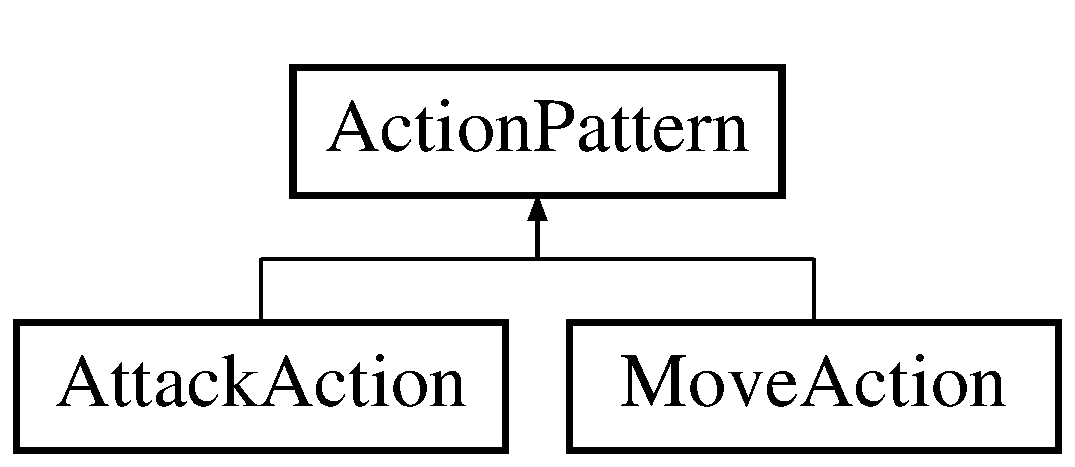
\includegraphics[height=2.000000cm]{class_action_pattern}
\end{center}
\end{figure}
\subsection*{公開メンバ関数}
\begin{DoxyCompactItemize}
\item 
virtual void \mbox{\hyperlink{class_action_pattern_ac8f2228ca469ce6fe29a9775bf393e0e}{Init}} ()=0
\item 
virtual std\+::shared\+\_\+ptr$<$ \mbox{\hyperlink{class_action_pattern}{Action\+Pattern}} $>$ \mbox{\hyperlink{class_action_pattern_a04c8daf0bf5e263303f7d86aec20eb27}{Action}} (std\+::shared\+\_\+ptr$<$ \mbox{\hyperlink{class_action_pattern}{Action\+Pattern}} $>$ \&, \mbox{\hyperlink{class_boss}{Boss}} \&, const float)=0
\item 
virtual void \mbox{\hyperlink{class_action_pattern_a313199aa5d15b6f9381b916ffe23fe6a}{Render}} ()=0
\item 
virtual void \mbox{\hyperlink{class_action_pattern_a73833df08867c4f4785ddf51344eca47}{Destroy}} ()=0
\item 
virtual \mbox{\hyperlink{class_action_pattern_a0549549b350f2a150835c07cb796131b}{$\sim$\+Action\+Pattern}} ()
\end{DoxyCompactItemize}


\subsection{構築子と解体子}
\mbox{\Hypertarget{class_action_pattern_a0549549b350f2a150835c07cb796131b}\label{class_action_pattern_a0549549b350f2a150835c07cb796131b}} 
\index{Action\+Pattern@{Action\+Pattern}!````~Action\+Pattern@{$\sim$\+Action\+Pattern}}
\index{````~Action\+Pattern@{$\sim$\+Action\+Pattern}!Action\+Pattern@{Action\+Pattern}}
\subsubsection{\texorpdfstring{$\sim$\+Action\+Pattern()}{~ActionPattern()}}
{\footnotesize\ttfamily virtual Action\+Pattern\+::$\sim$\+Action\+Pattern (\begin{DoxyParamCaption}{ }\end{DoxyParamCaption})\hspace{0.3cm}{\ttfamily [inline]}, {\ttfamily [virtual]}}



\subsection{関数詳解}
\mbox{\Hypertarget{class_action_pattern_a04c8daf0bf5e263303f7d86aec20eb27}\label{class_action_pattern_a04c8daf0bf5e263303f7d86aec20eb27}} 
\index{Action\+Pattern@{Action\+Pattern}!Action@{Action}}
\index{Action@{Action}!Action\+Pattern@{Action\+Pattern}}
\subsubsection{\texorpdfstring{Action()}{Action()}}
{\footnotesize\ttfamily virtual std\+::shared\+\_\+ptr$<$\mbox{\hyperlink{class_action_pattern}{Action\+Pattern}}$>$ Action\+Pattern\+::\+Action (\begin{DoxyParamCaption}\item[{std\+::shared\+\_\+ptr$<$ \mbox{\hyperlink{class_action_pattern}{Action\+Pattern}} $>$ \&}]{,  }\item[{\mbox{\hyperlink{class_boss}{Boss}} \&}]{,  }\item[{const float}]{ }\end{DoxyParamCaption})\hspace{0.3cm}{\ttfamily [pure virtual]}}



\mbox{\hyperlink{class_attack_action_a3e503ef3d5497f8a49a5273425c79476}{Attack\+Action}}, \mbox{\hyperlink{class_move_action_aa731fa679786c8c61965dfcd258c6c66}{Move\+Action}}で実装されています。

\mbox{\Hypertarget{class_action_pattern_a73833df08867c4f4785ddf51344eca47}\label{class_action_pattern_a73833df08867c4f4785ddf51344eca47}} 
\index{Action\+Pattern@{Action\+Pattern}!Destroy@{Destroy}}
\index{Destroy@{Destroy}!Action\+Pattern@{Action\+Pattern}}
\subsubsection{\texorpdfstring{Destroy()}{Destroy()}}
{\footnotesize\ttfamily virtual void Action\+Pattern\+::\+Destroy (\begin{DoxyParamCaption}{ }\end{DoxyParamCaption})\hspace{0.3cm}{\ttfamily [pure virtual]}}



\mbox{\hyperlink{class_attack_action_aa91f60f80fc0c76f321fbf2da3945c43}{Attack\+Action}}, \mbox{\hyperlink{class_move_action_a48727a426f2a69ed62631af8385ff6ef}{Move\+Action}}で実装されています。

\mbox{\Hypertarget{class_action_pattern_ac8f2228ca469ce6fe29a9775bf393e0e}\label{class_action_pattern_ac8f2228ca469ce6fe29a9775bf393e0e}} 
\index{Action\+Pattern@{Action\+Pattern}!Init@{Init}}
\index{Init@{Init}!Action\+Pattern@{Action\+Pattern}}
\subsubsection{\texorpdfstring{Init()}{Init()}}
{\footnotesize\ttfamily virtual void Action\+Pattern\+::\+Init (\begin{DoxyParamCaption}{ }\end{DoxyParamCaption})\hspace{0.3cm}{\ttfamily [pure virtual]}}



\mbox{\hyperlink{class_attack_action_afd8d8c674040a1361c35d1703f36b30e}{Attack\+Action}}, \mbox{\hyperlink{class_move_action_a0861a4a0fcbab38f8c33ed02b9f3c1b8}{Move\+Action}}で実装されています。

\mbox{\Hypertarget{class_action_pattern_a313199aa5d15b6f9381b916ffe23fe6a}\label{class_action_pattern_a313199aa5d15b6f9381b916ffe23fe6a}} 
\index{Action\+Pattern@{Action\+Pattern}!Render@{Render}}
\index{Render@{Render}!Action\+Pattern@{Action\+Pattern}}
\subsubsection{\texorpdfstring{Render()}{Render()}}
{\footnotesize\ttfamily virtual void Action\+Pattern\+::\+Render (\begin{DoxyParamCaption}{ }\end{DoxyParamCaption})\hspace{0.3cm}{\ttfamily [pure virtual]}}



\mbox{\hyperlink{class_attack_action_a779cc8743807e3e5d01cb3dd14f92bd7}{Attack\+Action}}, \mbox{\hyperlink{class_move_action_a3f427440c2409e0633ff0f6040a0320c}{Move\+Action}}で実装されています。



このクラス詳解は次のファイルから抽出されました\+:\begin{DoxyCompactItemize}
\item 
C\+:/\+Users/tokir/\+Documents/\+Git\+Hub/\+Weapon\+Merchant\+Adventure/src/src/object/character/enemy/boss/action\+\_\+pattern/base/\mbox{\hyperlink{action__pattern__base_8h}{action\+\_\+pattern\+\_\+base.\+h}}\end{DoxyCompactItemize}

\hypertarget{class_action_pattern_manager}{}\section{Action\+Pattern\+Manager クラス}
\label{class_action_pattern_manager}\index{Action\+Pattern\+Manager@{Action\+Pattern\+Manager}}


{\ttfamily \#include $<$action\+\_\+pattern\+\_\+manager.\+h$>$}

\subsection*{公開メンバ関数}
\begin{DoxyCompactItemize}
\item 
\mbox{\hyperlink{class_action_pattern_manager_a5bec0e724b77bbe2acb3ff62c7c8644d}{Action\+Pattern\+Manager}} (\mbox{\hyperlink{class_boss}{Boss}} \&)
\item 
void \mbox{\hyperlink{class_action_pattern_manager_a0cefb944b14e16b805b549831a8c060b}{Update}} (const float)
\item 
void \mbox{\hyperlink{class_action_pattern_manager_a094e2e5e3bbaf87e597b41b074ba2bd3}{Render}} ()
\item 
void \mbox{\hyperlink{class_action_pattern_manager_a24ae5b706adcb376c222703c55396c03}{Destroy}} ()
\end{DoxyCompactItemize}


\subsection{構築子と解体子}
\mbox{\Hypertarget{class_action_pattern_manager_a5bec0e724b77bbe2acb3ff62c7c8644d}\label{class_action_pattern_manager_a5bec0e724b77bbe2acb3ff62c7c8644d}} 
\index{Action\+Pattern\+Manager@{Action\+Pattern\+Manager}!Action\+Pattern\+Manager@{Action\+Pattern\+Manager}}
\index{Action\+Pattern\+Manager@{Action\+Pattern\+Manager}!Action\+Pattern\+Manager@{Action\+Pattern\+Manager}}
\subsubsection{\texorpdfstring{Action\+Pattern\+Manager()}{ActionPatternManager()}}
{\footnotesize\ttfamily Action\+Pattern\+Manager\+::\+Action\+Pattern\+Manager (\begin{DoxyParamCaption}\item[{\mbox{\hyperlink{class_boss}{Boss}} \&}]{\+\_\+boss }\end{DoxyParamCaption})}



\subsection{関数詳解}
\mbox{\Hypertarget{class_action_pattern_manager_a24ae5b706adcb376c222703c55396c03}\label{class_action_pattern_manager_a24ae5b706adcb376c222703c55396c03}} 
\index{Action\+Pattern\+Manager@{Action\+Pattern\+Manager}!Destroy@{Destroy}}
\index{Destroy@{Destroy}!Action\+Pattern\+Manager@{Action\+Pattern\+Manager}}
\subsubsection{\texorpdfstring{Destroy()}{Destroy()}}
{\footnotesize\ttfamily void Action\+Pattern\+Manager\+::\+Destroy (\begin{DoxyParamCaption}{ }\end{DoxyParamCaption})}

\mbox{\Hypertarget{class_action_pattern_manager_a094e2e5e3bbaf87e597b41b074ba2bd3}\label{class_action_pattern_manager_a094e2e5e3bbaf87e597b41b074ba2bd3}} 
\index{Action\+Pattern\+Manager@{Action\+Pattern\+Manager}!Render@{Render}}
\index{Render@{Render}!Action\+Pattern\+Manager@{Action\+Pattern\+Manager}}
\subsubsection{\texorpdfstring{Render()}{Render()}}
{\footnotesize\ttfamily void Action\+Pattern\+Manager\+::\+Render (\begin{DoxyParamCaption}{ }\end{DoxyParamCaption})}

\mbox{\Hypertarget{class_action_pattern_manager_a0cefb944b14e16b805b549831a8c060b}\label{class_action_pattern_manager_a0cefb944b14e16b805b549831a8c060b}} 
\index{Action\+Pattern\+Manager@{Action\+Pattern\+Manager}!Update@{Update}}
\index{Update@{Update}!Action\+Pattern\+Manager@{Action\+Pattern\+Manager}}
\subsubsection{\texorpdfstring{Update()}{Update()}}
{\footnotesize\ttfamily void Action\+Pattern\+Manager\+::\+Update (\begin{DoxyParamCaption}\item[{const float}]{x }\end{DoxyParamCaption})}



このクラス詳解は次のファイルから抽出されました\+:\begin{DoxyCompactItemize}
\item 
C\+:/\+Users/tokir/\+Documents/\+Git\+Hub/\+Weapon\+Merchant\+Adventure/src/src/object/character/enemy/boss/manager/\mbox{\hyperlink{action__pattern__manager_8h}{action\+\_\+pattern\+\_\+manager.\+h}}\item 
C\+:/\+Users/tokir/\+Documents/\+Git\+Hub/\+Weapon\+Merchant\+Adventure/src/src/object/character/enemy/boss/manager/\mbox{\hyperlink{action__pattern__manager_8cpp}{action\+\_\+pattern\+\_\+manager.\+cpp}}\end{DoxyCompactItemize}

\hypertarget{structsaki_1_1addition}{}\section{saki\+:\+:addition 構造体}
\label{structsaki_1_1addition}\index{saki\+::addition@{saki\+::addition}}


足し算のconstexpr対応した関数オブジェクト  




{\ttfamily \#include $<$addition.\+h$>$}

\subsection*{公開メンバ関数}
\begin{DoxyCompactItemize}
\item 
{\footnotesize template$<$typename T1 , typename T2 $>$ }\\constexpr auto \mbox{\hyperlink{structsaki_1_1addition_a8bdb3c15f72b4d0f48967fdaa1472049}{operator()}} (const T1 \&t1, const T2 \&t2) const
\end{DoxyCompactItemize}


\subsection{詳解}
足し算のconstexpr対応した関数オブジェクト 

\subsection{関数詳解}
\mbox{\Hypertarget{structsaki_1_1addition_a8bdb3c15f72b4d0f48967fdaa1472049}\label{structsaki_1_1addition_a8bdb3c15f72b4d0f48967fdaa1472049}} 
\index{saki\+::addition@{saki\+::addition}!operator()@{operator()}}
\index{operator()@{operator()}!saki\+::addition@{saki\+::addition}}
\subsubsection{\texorpdfstring{operator()()}{operator()()}}
{\footnotesize\ttfamily template$<$typename T1 , typename T2 $>$ \\
constexpr auto saki\+::addition\+::operator() (\begin{DoxyParamCaption}\item[{const T1 \&}]{t1,  }\item[{const T2 \&}]{t2 }\end{DoxyParamCaption}) const\hspace{0.3cm}{\ttfamily [inline]}}



この構造体詳解は次のファイルから抽出されました\+:\begin{DoxyCompactItemize}
\item 
C\+:/\+Users/tokir/\+Documents/\+Git\+Hub/\+Weapon\+Merchant\+Adventure/src/lib/saki/binary\+\_\+operator/\mbox{\hyperlink{addition_8h}{addition.\+h}}\end{DoxyCompactItemize}

\hypertarget{class_animation}{}\section{Animation クラス}
\label{class_animation}\index{Animation@{Animation}}


アニメーションクラス  




{\ttfamily \#include $<$animation.\+h$>$}

\subsection*{公開メンバ関数}
\begin{DoxyCompactItemize}
\item 
\mbox{\hyperlink{class_animation_a83f0a16cef7117f187ad596de38dd9d6}{Animation}} ()
\item 
void \mbox{\hyperlink{class_animation_a6f532d6251cdf027ee8e6af311832c2f}{Changetime}} (const int t)
\item 
\mbox{\hyperlink{class_animation_a7c1388a1e58fb80682aa8e147f58d592}{Animation}} (const \mbox{\hyperlink{class_animation}{Animation}} \&other)
\begin{DoxyCompactList}\small\item\em コピーコンストラクタ \end{DoxyCompactList}\item 
\mbox{\hyperlink{class_animation}{Animation}} \& \mbox{\hyperlink{class_animation_a83fe682e706c6e5cc348b52bc8dbcddd}{operator=}} (const \mbox{\hyperlink{class_animation}{Animation}} \&other)
\begin{DoxyCompactList}\small\item\em コピー代入演算子 \end{DoxyCompactList}\item 
void \mbox{\hyperlink{class_animation_a3f62687a696758fdba6eb1810e971c0d}{Init}} (const \mbox{\hyperlink{common_8h_ae148fff5818e9444b4ab2288829559bf}{Vec2}} \&, const int, const int, const int)
\begin{DoxyCompactList}\small\item\em 初期化 \end{DoxyCompactList}\item 
void \mbox{\hyperlink{class_animation_a0c6a4e940db84d4a6246fcb3ae773402}{Update}} ()
\begin{DoxyCompactList}\small\item\em 更新 \end{DoxyCompactList}\item 
\mbox{\hyperlink{common_8h_ae148fff5818e9444b4ab2288829559bf}{Vec2}} \mbox{\hyperlink{class_animation_a313060e5a143cb24d0264744249fddd6}{Get\+Animation}} () const
\begin{DoxyCompactList}\small\item\em アニメーションを変更する \end{DoxyCompactList}\item 
void \mbox{\hyperlink{class_animation_ae9fe84bd92b1df395dd09aeed37a8373}{Change\+Animation}} (const int, const int, const bool=false)
\begin{DoxyCompactList}\small\item\em アニメーションを変える \end{DoxyCompactList}\end{DoxyCompactItemize}


\subsection{詳解}
アニメーションクラス 

\subsection{構築子と解体子}
\mbox{\Hypertarget{class_animation_a83f0a16cef7117f187ad596de38dd9d6}\label{class_animation_a83f0a16cef7117f187ad596de38dd9d6}} 
\index{Animation@{Animation}!Animation@{Animation}}
\index{Animation@{Animation}!Animation@{Animation}}
\subsubsection{\texorpdfstring{Animation()}{Animation()}\hspace{0.1cm}{\footnotesize\ttfamily [1/2]}}
{\footnotesize\ttfamily Animation\+::\+Animation (\begin{DoxyParamCaption}{ }\end{DoxyParamCaption})\hspace{0.3cm}{\ttfamily [inline]}}

\mbox{\Hypertarget{class_animation_a7c1388a1e58fb80682aa8e147f58d592}\label{class_animation_a7c1388a1e58fb80682aa8e147f58d592}} 
\index{Animation@{Animation}!Animation@{Animation}}
\index{Animation@{Animation}!Animation@{Animation}}
\subsubsection{\texorpdfstring{Animation()}{Animation()}\hspace{0.1cm}{\footnotesize\ttfamily [2/2]}}
{\footnotesize\ttfamily Animation\+::\+Animation (\begin{DoxyParamCaption}\item[{const \mbox{\hyperlink{class_animation}{Animation}} \&}]{other }\end{DoxyParamCaption})\hspace{0.3cm}{\ttfamily [inline]}}



コピーコンストラクタ 



\subsection{関数詳解}
\mbox{\Hypertarget{class_animation_ae9fe84bd92b1df395dd09aeed37a8373}\label{class_animation_ae9fe84bd92b1df395dd09aeed37a8373}} 
\index{Animation@{Animation}!Change\+Animation@{Change\+Animation}}
\index{Change\+Animation@{Change\+Animation}!Animation@{Animation}}
\subsubsection{\texorpdfstring{Change\+Animation()}{ChangeAnimation()}}
{\footnotesize\ttfamily void Animation\+::\+Change\+Animation (\begin{DoxyParamCaption}\item[{const int}]{vertical,  }\item[{const int}]{\+\_\+time,  }\item[{const bool}]{reset = {\ttfamily false} }\end{DoxyParamCaption})}



アニメーションを変える 


\begin{DoxyParams}{引数}
{\em vertical} & 上から何番目のアニメーションにするか(0スタート) \\
\hline
{\em \+\_\+time} & 何フレームごとに変更するか \\
\hline
{\em reset} & アニメーションを最初からするかどうか \\
\hline
\end{DoxyParams}
\mbox{\Hypertarget{class_animation_a6f532d6251cdf027ee8e6af311832c2f}\label{class_animation_a6f532d6251cdf027ee8e6af311832c2f}} 
\index{Animation@{Animation}!Changetime@{Changetime}}
\index{Changetime@{Changetime}!Animation@{Animation}}
\subsubsection{\texorpdfstring{Changetime()}{Changetime()}}
{\footnotesize\ttfamily void Animation\+::\+Changetime (\begin{DoxyParamCaption}\item[{const int}]{t }\end{DoxyParamCaption})\hspace{0.3cm}{\ttfamily [inline]}}

\mbox{\Hypertarget{class_animation_a313060e5a143cb24d0264744249fddd6}\label{class_animation_a313060e5a143cb24d0264744249fddd6}} 
\index{Animation@{Animation}!Get\+Animation@{Get\+Animation}}
\index{Get\+Animation@{Get\+Animation}!Animation@{Animation}}
\subsubsection{\texorpdfstring{Get\+Animation()}{GetAnimation()}}
{\footnotesize\ttfamily \mbox{\hyperlink{common_8h_ae148fff5818e9444b4ab2288829559bf}{Vec2}} Animation\+::\+Get\+Animation (\begin{DoxyParamCaption}{ }\end{DoxyParamCaption}) const}



アニメーションを変更する 

\begin{DoxyReturn}{戻り値}
R\+E\+CT テクスチャで描画する部分 
\end{DoxyReturn}
\mbox{\Hypertarget{class_animation_a3f62687a696758fdba6eb1810e971c0d}\label{class_animation_a3f62687a696758fdba6eb1810e971c0d}} 
\index{Animation@{Animation}!Init@{Init}}
\index{Init@{Init}!Animation@{Animation}}
\subsubsection{\texorpdfstring{Init()}{Init()}}
{\footnotesize\ttfamily void Animation\+::\+Init (\begin{DoxyParamCaption}\item[{const \mbox{\hyperlink{common_8h_ae148fff5818e9444b4ab2288829559bf}{Vec2}} \&}]{\+\_\+one,  }\item[{const int}]{hor,  }\item[{const int}]{ver,  }\item[{const int}]{\+\_\+inter }\end{DoxyParamCaption})}



初期化 


\begin{DoxyParams}{引数}
{\em \+\_\+one} & 一つ当たりの大きさ \\
\hline
{\em hor} & 横の数 \\
\hline
{\em ver} & 縦の数 \\
\hline
{\em \+\_\+inter} & 一つ一つの間隔 \\
\hline
\end{DoxyParams}
\mbox{\Hypertarget{class_animation_a83fe682e706c6e5cc348b52bc8dbcddd}\label{class_animation_a83fe682e706c6e5cc348b52bc8dbcddd}} 
\index{Animation@{Animation}!operator=@{operator=}}
\index{operator=@{operator=}!Animation@{Animation}}
\subsubsection{\texorpdfstring{operator=()}{operator=()}}
{\footnotesize\ttfamily \mbox{\hyperlink{class_animation}{Animation}}\& Animation\+::operator= (\begin{DoxyParamCaption}\item[{const \mbox{\hyperlink{class_animation}{Animation}} \&}]{other }\end{DoxyParamCaption})\hspace{0.3cm}{\ttfamily [inline]}}



コピー代入演算子 

\mbox{\Hypertarget{class_animation_a0c6a4e940db84d4a6246fcb3ae773402}\label{class_animation_a0c6a4e940db84d4a6246fcb3ae773402}} 
\index{Animation@{Animation}!Update@{Update}}
\index{Update@{Update}!Animation@{Animation}}
\subsubsection{\texorpdfstring{Update()}{Update()}}
{\footnotesize\ttfamily void Animation\+::\+Update (\begin{DoxyParamCaption}{ }\end{DoxyParamCaption})}



更新 



このクラス詳解は次のファイルから抽出されました\+:\begin{DoxyCompactItemize}
\item 
C\+:/\+Users/tokir/\+Documents/\+Git\+Hub/\+Weapon\+Merchant\+Adventure/src/src/animation/\mbox{\hyperlink{animation_8h}{animation.\+h}}\item 
C\+:/\+Users/tokir/\+Documents/\+Git\+Hub/\+Weapon\+Merchant\+Adventure/src/src/animation/\mbox{\hyperlink{animation_8cpp}{animation.\+cpp}}\end{DoxyCompactItemize}

\hypertarget{class_arrow}{}\section{Arrow クラス}
\label{class_arrow}\index{Arrow@{Arrow}}


遠距離武器クラス  




{\ttfamily \#include $<$arrow.\+h$>$}

Arrow の継承関係図\begin{figure}[H]
\begin{center}
\leavevmode
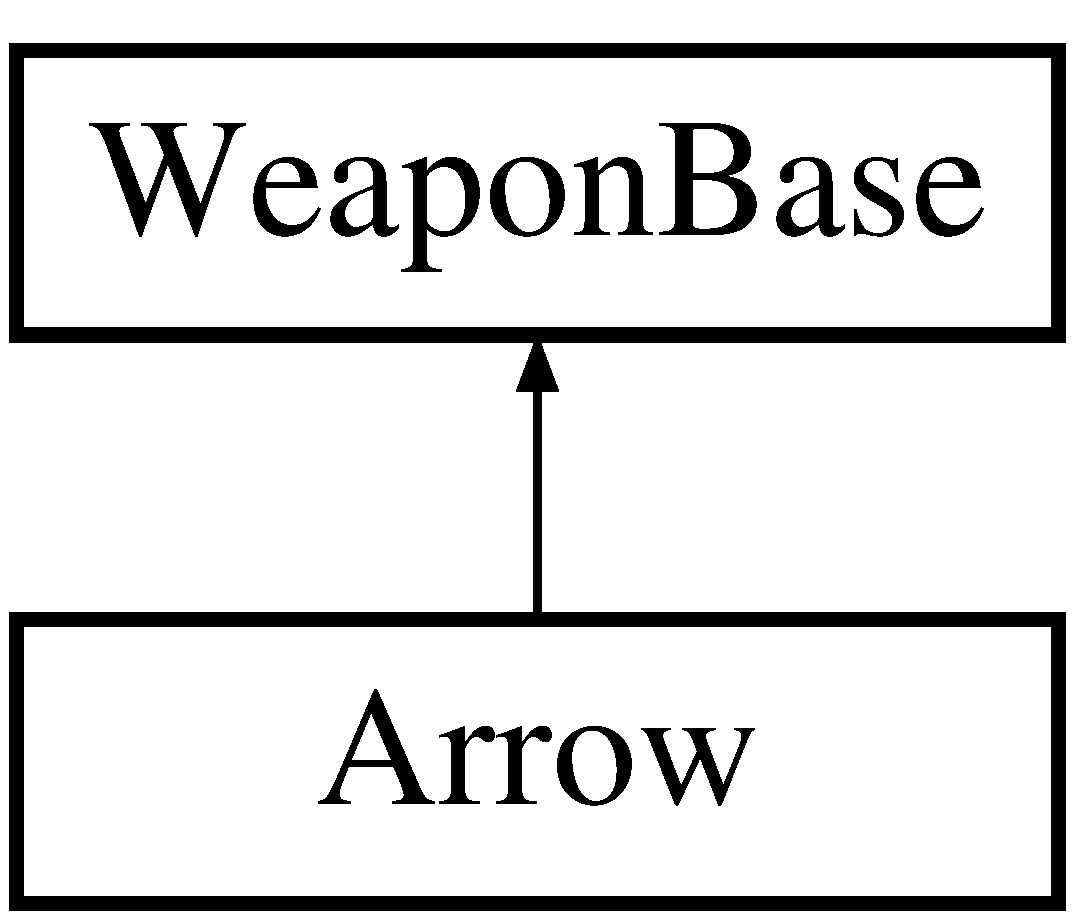
\includegraphics[height=2.000000cm]{class_arrow}
\end{center}
\end{figure}
\subsection*{公開メンバ関数}
\begin{DoxyCompactItemize}
\item 
void \mbox{\hyperlink{class_arrow_afe567fd69597c0a5c44edd99c06d6f71}{Collision\+Bullet}} ()
\begin{DoxyCompactList}\small\item\em 弾が当たったときに実行する関数 \end{DoxyCompactList}\item 
bool \mbox{\hyperlink{class_arrow_a98ea469bf0b21635b2d2dadb69c72240}{Attack}} (bool, const \mbox{\hyperlink{common_8h_ab1cb35b3a17c398d8ef71d5f779808bf}{Vec3}} \&) final
\begin{DoxyCompactList}\small\item\em 攻撃 \end{DoxyCompactList}\item 
void \mbox{\hyperlink{class_arrow_a085b5bd5f9e3ce25a081b502f9989f33}{Weapon\+Start}} () final
\begin{DoxyCompactList}\small\item\em 武器用の初期化 \end{DoxyCompactList}\item 
void \mbox{\hyperlink{class_arrow_afb6110035cba7b850d12755570163b29}{Weapon\+Update}} (const \mbox{\hyperlink{common_8h_ab1cb35b3a17c398d8ef71d5f779808bf}{Vec3}} \&, bool=true) final
\begin{DoxyCompactList}\small\item\em 武器の更新 \end{DoxyCompactList}\item 
void \mbox{\hyperlink{class_arrow_af9e54760156a77a15ad98a88f712ebdb}{Weapon\+Render}} (const \mbox{\hyperlink{common_8h_a1c43cb8f0d8a41901f3ce4c67dbbce20}{Transform}} \&=\mbox{\hyperlink{common_8h_a1c43cb8f0d8a41901f3ce4c67dbbce20}{Transform}}\{ saki\+::vector3\+\_\+zero$<$ float $>$, saki\+::vector3\+\_\+zero$<$ float $>$, saki\+::vector3\+\_\+zero$<$ float $>$ \}) final
\begin{DoxyCompactList}\small\item\em 武器の描画 \end{DoxyCompactList}\item 
void \mbox{\hyperlink{class_arrow_a1101d1159771b5c428afd3c7a6a0a4df}{Weapon\+Destroy}} () final
\begin{DoxyCompactList}\small\item\em 武器の破棄 \end{DoxyCompactList}\end{DoxyCompactItemize}
\subsection*{その他の継承メンバ}


\subsection{詳解}
遠距離武器クラス 

\subsection{関数詳解}
\mbox{\Hypertarget{class_arrow_a98ea469bf0b21635b2d2dadb69c72240}\label{class_arrow_a98ea469bf0b21635b2d2dadb69c72240}} 
\index{Arrow@{Arrow}!Attack@{Attack}}
\index{Attack@{Attack}!Arrow@{Arrow}}
\subsubsection{\texorpdfstring{Attack()}{Attack()}}
{\footnotesize\ttfamily bool Arrow\+::\+Attack (\begin{DoxyParamCaption}\item[{bool}]{right,  }\item[{const \mbox{\hyperlink{common_8h_ab1cb35b3a17c398d8ef71d5f779808bf}{Vec3}} \&}]{pos }\end{DoxyParamCaption})\hspace{0.3cm}{\ttfamily [final]}, {\ttfamily [virtual]}}



攻撃 


\begin{DoxyParams}{引数}
{\em right} & 右かどうか \\
\hline
{\em pos} & 弾を発射する位置 \\
\hline
\end{DoxyParams}


\mbox{\hyperlink{class_weapon_base_a1bab9c7fb9524db754bebbbcbf6c2fd9}{Weapon\+Base}}を実装しています。

\mbox{\Hypertarget{class_arrow_afe567fd69597c0a5c44edd99c06d6f71}\label{class_arrow_afe567fd69597c0a5c44edd99c06d6f71}} 
\index{Arrow@{Arrow}!Collision\+Bullet@{Collision\+Bullet}}
\index{Collision\+Bullet@{Collision\+Bullet}!Arrow@{Arrow}}
\subsubsection{\texorpdfstring{Collision\+Bullet()}{CollisionBullet()}}
{\footnotesize\ttfamily void Arrow\+::\+Collision\+Bullet (\begin{DoxyParamCaption}{ }\end{DoxyParamCaption})}



弾が当たったときに実行する関数 

\mbox{\Hypertarget{class_arrow_a1101d1159771b5c428afd3c7a6a0a4df}\label{class_arrow_a1101d1159771b5c428afd3c7a6a0a4df}} 
\index{Arrow@{Arrow}!Weapon\+Destroy@{Weapon\+Destroy}}
\index{Weapon\+Destroy@{Weapon\+Destroy}!Arrow@{Arrow}}
\subsubsection{\texorpdfstring{Weapon\+Destroy()}{WeaponDestroy()}}
{\footnotesize\ttfamily void Arrow\+::\+Weapon\+Destroy (\begin{DoxyParamCaption}{ }\end{DoxyParamCaption})\hspace{0.3cm}{\ttfamily [final]}, {\ttfamily [virtual]}}



武器の破棄 



\mbox{\hyperlink{class_weapon_base_a417784a8c8bf73cd398a77b922fc110c}{Weapon\+Base}}を実装しています。

\mbox{\Hypertarget{class_arrow_af9e54760156a77a15ad98a88f712ebdb}\label{class_arrow_af9e54760156a77a15ad98a88f712ebdb}} 
\index{Arrow@{Arrow}!Weapon\+Render@{Weapon\+Render}}
\index{Weapon\+Render@{Weapon\+Render}!Arrow@{Arrow}}
\subsubsection{\texorpdfstring{Weapon\+Render()}{WeaponRender()}}
{\footnotesize\ttfamily void Arrow\+::\+Weapon\+Render (\begin{DoxyParamCaption}\item[{const \mbox{\hyperlink{common_8h_a1c43cb8f0d8a41901f3ce4c67dbbce20}{Transform}} \&}]{ = {\ttfamily \mbox{\hyperlink{common_8h_a1c43cb8f0d8a41901f3ce4c67dbbce20}{Transform}}\{~saki\+:\+:vector3\+\_\+zero$<$float$>$,saki\+:\+:vector3\+\_\+zero$<$float$>$,saki\+:\+:vector3\+\_\+zero$<$float$>$~\}} }\end{DoxyParamCaption})\hspace{0.3cm}{\ttfamily [final]}, {\ttfamily [virtual]}}



武器の描画 


\begin{DoxyParams}{引数}
{\em t} & 描画位置 \\
\hline
\end{DoxyParams}


\mbox{\hyperlink{class_weapon_base_af308d16d3892c3ffaeedf74b08e761b9}{Weapon\+Base}}を実装しています。

\mbox{\Hypertarget{class_arrow_a085b5bd5f9e3ce25a081b502f9989f33}\label{class_arrow_a085b5bd5f9e3ce25a081b502f9989f33}} 
\index{Arrow@{Arrow}!Weapon\+Start@{Weapon\+Start}}
\index{Weapon\+Start@{Weapon\+Start}!Arrow@{Arrow}}
\subsubsection{\texorpdfstring{Weapon\+Start()}{WeaponStart()}}
{\footnotesize\ttfamily void Arrow\+::\+Weapon\+Start (\begin{DoxyParamCaption}{ }\end{DoxyParamCaption})\hspace{0.3cm}{\ttfamily [final]}, {\ttfamily [virtual]}}



武器用の初期化 



\mbox{\hyperlink{class_weapon_base_a25cd4c351638b76377e93341a9545712}{Weapon\+Base}}を実装しています。

\mbox{\Hypertarget{class_arrow_afb6110035cba7b850d12755570163b29}\label{class_arrow_afb6110035cba7b850d12755570163b29}} 
\index{Arrow@{Arrow}!Weapon\+Update@{Weapon\+Update}}
\index{Weapon\+Update@{Weapon\+Update}!Arrow@{Arrow}}
\subsubsection{\texorpdfstring{Weapon\+Update()}{WeaponUpdate()}}
{\footnotesize\ttfamily void Arrow\+::\+Weapon\+Update (\begin{DoxyParamCaption}\item[{const \mbox{\hyperlink{common_8h_ab1cb35b3a17c398d8ef71d5f779808bf}{Vec3}} \&}]{,  }\item[{bool}]{ = {\ttfamily true} }\end{DoxyParamCaption})\hspace{0.3cm}{\ttfamily [final]}, {\ttfamily [virtual]}}



武器の更新 



\mbox{\hyperlink{class_weapon_base_aa1e3d02353273ab72a71cc3a1563636a}{Weapon\+Base}}を実装しています。



このクラス詳解は次のファイルから抽出されました\+:\begin{DoxyCompactItemize}
\item 
C\+:/\+Users/tokir/\+Documents/\+Git\+Hub/\+Weapon\+Merchant\+Adventure/src/src/object/weapon/arrow/\mbox{\hyperlink{arrow_8h}{arrow.\+h}}\item 
C\+:/\+Users/tokir/\+Documents/\+Git\+Hub/\+Weapon\+Merchant\+Adventure/src/src/object/weapon/arrow/\mbox{\hyperlink{arrow_8cpp}{arrow.\+cpp}}\end{DoxyCompactItemize}

\hypertarget{class_attack_action}{}\section{Attack\+Action クラス}
\label{class_attack_action}\index{Attack\+Action@{Attack\+Action}}


{\ttfamily \#include $<$attack\+\_\+action.\+h$>$}

Attack\+Action の継承関係図\begin{figure}[H]
\begin{center}
\leavevmode
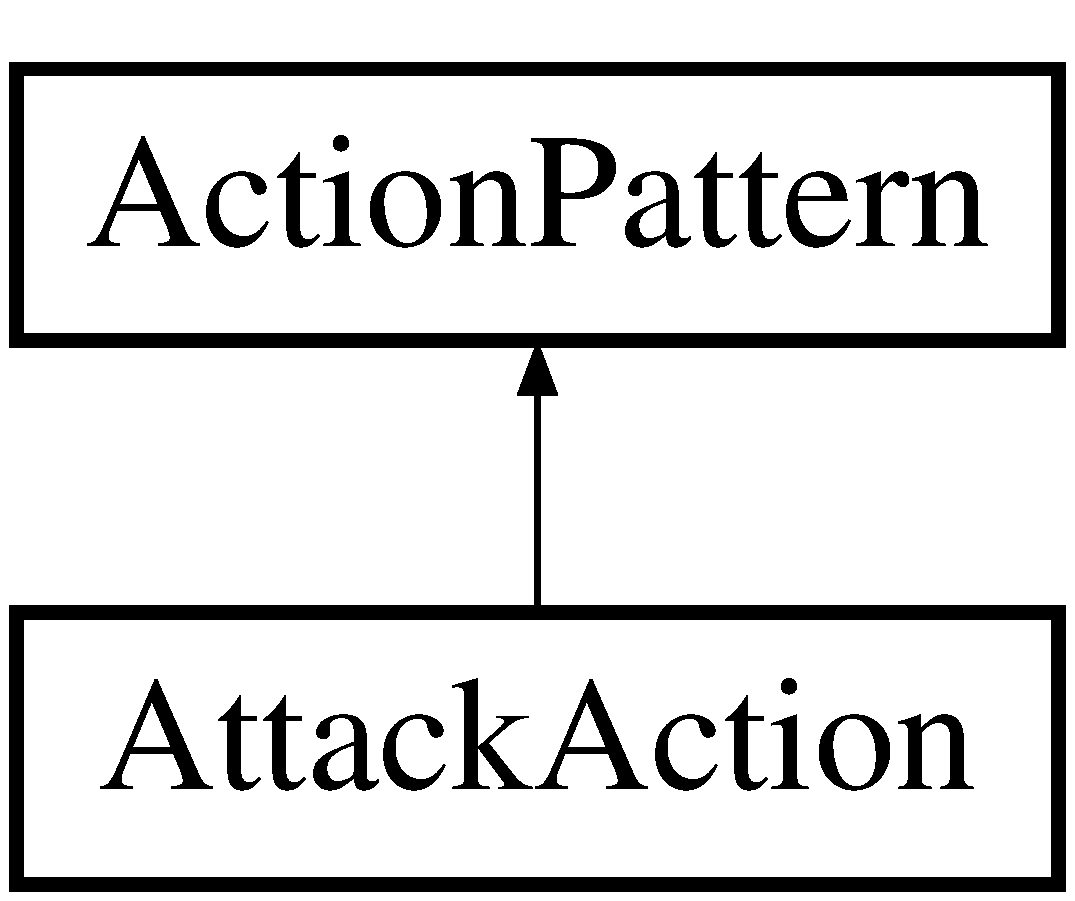
\includegraphics[height=2.000000cm]{class_attack_action}
\end{center}
\end{figure}
\subsection*{公開メンバ関数}
\begin{DoxyCompactItemize}
\item 
void \mbox{\hyperlink{class_attack_action_afd8d8c674040a1361c35d1703f36b30e}{Init}} () final
\item 
std\+::shared\+\_\+ptr$<$ \mbox{\hyperlink{class_action_pattern}{Action\+Pattern}} $>$ \mbox{\hyperlink{class_attack_action_a3e503ef3d5497f8a49a5273425c79476}{Action}} (std\+::shared\+\_\+ptr$<$ \mbox{\hyperlink{class_action_pattern}{Action\+Pattern}} $>$ \&, \mbox{\hyperlink{class_boss}{Boss}} \&, const float) final
\item 
void \mbox{\hyperlink{class_attack_action_a779cc8743807e3e5d01cb3dd14f92bd7}{Render}} () final
\item 
void \mbox{\hyperlink{class_attack_action_aa91f60f80fc0c76f321fbf2da3945c43}{Destroy}} () final
\end{DoxyCompactItemize}


\subsection{関数詳解}
\mbox{\Hypertarget{class_attack_action_a3e503ef3d5497f8a49a5273425c79476}\label{class_attack_action_a3e503ef3d5497f8a49a5273425c79476}} 
\index{Attack\+Action@{Attack\+Action}!Action@{Action}}
\index{Action@{Action}!Attack\+Action@{Attack\+Action}}
\subsubsection{\texorpdfstring{Action()}{Action()}}
{\footnotesize\ttfamily std\+::shared\+\_\+ptr$<$ \mbox{\hyperlink{class_action_pattern}{Action\+Pattern}} $>$ Attack\+Action\+::\+Action (\begin{DoxyParamCaption}\item[{std\+::shared\+\_\+ptr$<$ \mbox{\hyperlink{class_action_pattern}{Action\+Pattern}} $>$ \&}]{action\+\_\+ptr,  }\item[{\mbox{\hyperlink{class_boss}{Boss}} \&}]{boss,  }\item[{const float}]{center\+\_\+pos\+\_\+x }\end{DoxyParamCaption})\hspace{0.3cm}{\ttfamily [final]}, {\ttfamily [virtual]}}



\mbox{\hyperlink{class_action_pattern_a04c8daf0bf5e263303f7d86aec20eb27}{Action\+Pattern}}を実装しています。

\mbox{\Hypertarget{class_attack_action_aa91f60f80fc0c76f321fbf2da3945c43}\label{class_attack_action_aa91f60f80fc0c76f321fbf2da3945c43}} 
\index{Attack\+Action@{Attack\+Action}!Destroy@{Destroy}}
\index{Destroy@{Destroy}!Attack\+Action@{Attack\+Action}}
\subsubsection{\texorpdfstring{Destroy()}{Destroy()}}
{\footnotesize\ttfamily void Attack\+Action\+::\+Destroy (\begin{DoxyParamCaption}{ }\end{DoxyParamCaption})\hspace{0.3cm}{\ttfamily [final]}, {\ttfamily [virtual]}}



\mbox{\hyperlink{class_action_pattern_a73833df08867c4f4785ddf51344eca47}{Action\+Pattern}}を実装しています。

\mbox{\Hypertarget{class_attack_action_afd8d8c674040a1361c35d1703f36b30e}\label{class_attack_action_afd8d8c674040a1361c35d1703f36b30e}} 
\index{Attack\+Action@{Attack\+Action}!Init@{Init}}
\index{Init@{Init}!Attack\+Action@{Attack\+Action}}
\subsubsection{\texorpdfstring{Init()}{Init()}}
{\footnotesize\ttfamily void Attack\+Action\+::\+Init (\begin{DoxyParamCaption}{ }\end{DoxyParamCaption})\hspace{0.3cm}{\ttfamily [final]}, {\ttfamily [virtual]}}



\mbox{\hyperlink{class_action_pattern_ac8f2228ca469ce6fe29a9775bf393e0e}{Action\+Pattern}}を実装しています。

\mbox{\Hypertarget{class_attack_action_a779cc8743807e3e5d01cb3dd14f92bd7}\label{class_attack_action_a779cc8743807e3e5d01cb3dd14f92bd7}} 
\index{Attack\+Action@{Attack\+Action}!Render@{Render}}
\index{Render@{Render}!Attack\+Action@{Attack\+Action}}
\subsubsection{\texorpdfstring{Render()}{Render()}}
{\footnotesize\ttfamily void Attack\+Action\+::\+Render (\begin{DoxyParamCaption}{ }\end{DoxyParamCaption})\hspace{0.3cm}{\ttfamily [final]}, {\ttfamily [virtual]}}



\mbox{\hyperlink{class_action_pattern_a313199aa5d15b6f9381b916ffe23fe6a}{Action\+Pattern}}を実装しています。



このクラス詳解は次のファイルから抽出されました\+:\begin{DoxyCompactItemize}
\item 
C\+:/\+Users/tokir/\+Documents/\+Git\+Hub/\+Weapon\+Merchant\+Adventure/src/src/object/character/enemy/boss/action\+\_\+pattern/attack/\mbox{\hyperlink{attack__action_8h}{attack\+\_\+action.\+h}}\item 
C\+:/\+Users/tokir/\+Documents/\+Git\+Hub/\+Weapon\+Merchant\+Adventure/src/src/object/character/enemy/boss/action\+\_\+pattern/attack/\mbox{\hyperlink{attack__action_8cpp}{attack\+\_\+action.\+cpp}}\end{DoxyCompactItemize}

\hypertarget{class_b_g_m}{}\section{B\+GM クラス}
\label{class_b_g_m}\index{B\+GM@{B\+GM}}


B\+G\+Mクラス  




{\ttfamily \#include $<$bgm.\+h$>$}

B\+GM の継承関係図\begin{figure}[H]
\begin{center}
\leavevmode
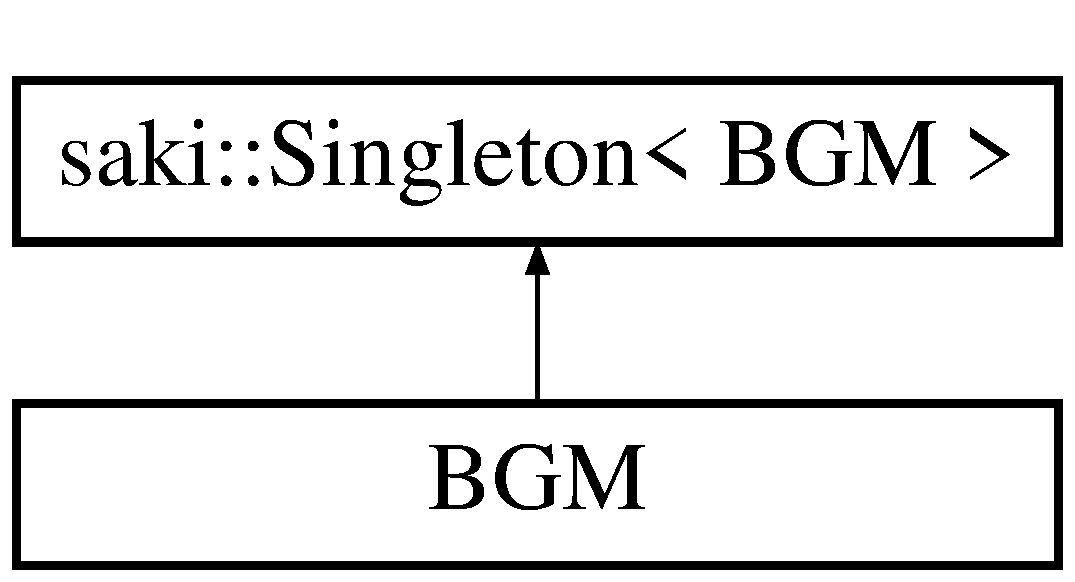
\includegraphics[height=2.000000cm]{class_b_g_m}
\end{center}
\end{figure}
\subsection*{公開メンバ関数}
\begin{DoxyCompactItemize}
\item 
void \mbox{\hyperlink{class_b_g_m_a63645262b99c4d3aef0a58d9b972f674}{Fade}} (const bool)
\begin{DoxyCompactList}\small\item\em 主にシーン遷移時になめらかに\+B\+G\+Mを変えるため \end{DoxyCompactList}\item 
void \mbox{\hyperlink{class_b_g_m_a67e626cf0e596ca4fcf74df02fadf882}{Change\+Bgm}} (const std\+::string \&, W\+C\+H\+AR $\ast$)
\begin{DoxyCompactList}\small\item\em B\+G\+Mを変える \end{DoxyCompactList}\item 
void \mbox{\hyperlink{class_b_g_m_a6d5d9eddf086075d2b579c3a8061cc8c}{Set\+Volume}} (const float v)
\item 
void \mbox{\hyperlink{class_b_g_m_a5aaf11289bdf7eddba2ee3af7995b4fc}{One\+Shot\+B\+GM}} (const std\+::string \&, W\+C\+H\+AR $\ast$)
\begin{DoxyCompactList}\small\item\em B\+G\+Mを変える(ループなし) \end{DoxyCompactList}\end{DoxyCompactItemize}
\subsection*{その他の継承メンバ}


\subsection{詳解}
B\+G\+Mクラス 

\subsection{関数詳解}
\mbox{\Hypertarget{class_b_g_m_a67e626cf0e596ca4fcf74df02fadf882}\label{class_b_g_m_a67e626cf0e596ca4fcf74df02fadf882}} 
\index{B\+GM@{B\+GM}!Change\+Bgm@{Change\+Bgm}}
\index{Change\+Bgm@{Change\+Bgm}!B\+GM@{B\+GM}}
\subsubsection{\texorpdfstring{Change\+Bgm()}{ChangeBgm()}}
{\footnotesize\ttfamily void B\+G\+M\+::\+Change\+Bgm (\begin{DoxyParamCaption}\item[{const std\+::string \&}]{name,  }\item[{W\+C\+H\+AR $\ast$}]{path }\end{DoxyParamCaption})}



B\+G\+Mを変える 


\begin{DoxyParams}{引数}
{\em name} & キー \\
\hline
{\em path} & パス \\
\hline
\end{DoxyParams}
\mbox{\Hypertarget{class_b_g_m_a63645262b99c4d3aef0a58d9b972f674}\label{class_b_g_m_a63645262b99c4d3aef0a58d9b972f674}} 
\index{B\+GM@{B\+GM}!Fade@{Fade}}
\index{Fade@{Fade}!B\+GM@{B\+GM}}
\subsubsection{\texorpdfstring{Fade()}{Fade()}}
{\footnotesize\ttfamily void B\+G\+M\+::\+Fade (\begin{DoxyParamCaption}\item[{const bool}]{fade\+\_\+in }\end{DoxyParamCaption})}



主にシーン遷移時になめらかに\+B\+G\+Mを変えるため 


\begin{DoxyParams}{引数}
{\em fade\+\_\+in} & フェードインかどうか \\
\hline
\end{DoxyParams}
\mbox{\Hypertarget{class_b_g_m_a5aaf11289bdf7eddba2ee3af7995b4fc}\label{class_b_g_m_a5aaf11289bdf7eddba2ee3af7995b4fc}} 
\index{B\+GM@{B\+GM}!One\+Shot\+B\+GM@{One\+Shot\+B\+GM}}
\index{One\+Shot\+B\+GM@{One\+Shot\+B\+GM}!B\+GM@{B\+GM}}
\subsubsection{\texorpdfstring{One\+Shot\+B\+G\+M()}{OneShotBGM()}}
{\footnotesize\ttfamily void B\+G\+M\+::\+One\+Shot\+B\+GM (\begin{DoxyParamCaption}\item[{const std\+::string \&}]{name,  }\item[{W\+C\+H\+AR $\ast$}]{path }\end{DoxyParamCaption})}



B\+G\+Mを変える(ループなし) 


\begin{DoxyParams}{引数}
{\em name} & キー \\
\hline
{\em path} & パス \\
\hline
\end{DoxyParams}
\mbox{\Hypertarget{class_b_g_m_a6d5d9eddf086075d2b579c3a8061cc8c}\label{class_b_g_m_a6d5d9eddf086075d2b579c3a8061cc8c}} 
\index{B\+GM@{B\+GM}!Set\+Volume@{Set\+Volume}}
\index{Set\+Volume@{Set\+Volume}!B\+GM@{B\+GM}}
\subsubsection{\texorpdfstring{Set\+Volume()}{SetVolume()}}
{\footnotesize\ttfamily void B\+G\+M\+::\+Set\+Volume (\begin{DoxyParamCaption}\item[{const float}]{v }\end{DoxyParamCaption})\hspace{0.3cm}{\ttfamily [inline]}}



このクラス詳解は次のファイルから抽出されました\+:\begin{DoxyCompactItemize}
\item 
C\+:/\+Users/tokir/\+Documents/\+Git\+Hub/\+Weapon\+Merchant\+Adventure/src/src/sound/bgm/\mbox{\hyperlink{bgm_8h}{bgm.\+h}}\item 
C\+:/\+Users/tokir/\+Documents/\+Git\+Hub/\+Weapon\+Merchant\+Adventure/src/src/sound/bgm/\mbox{\hyperlink{bgm_8cpp}{bgm.\+cpp}}\end{DoxyCompactItemize}

\hypertarget{class_boss}{}\section{Boss クラス}
\label{class_boss}\index{Boss@{Boss}}


{\ttfamily \#include $<$boss.\+h$>$}

Boss の継承関係図\begin{figure}[H]
\begin{center}
\leavevmode
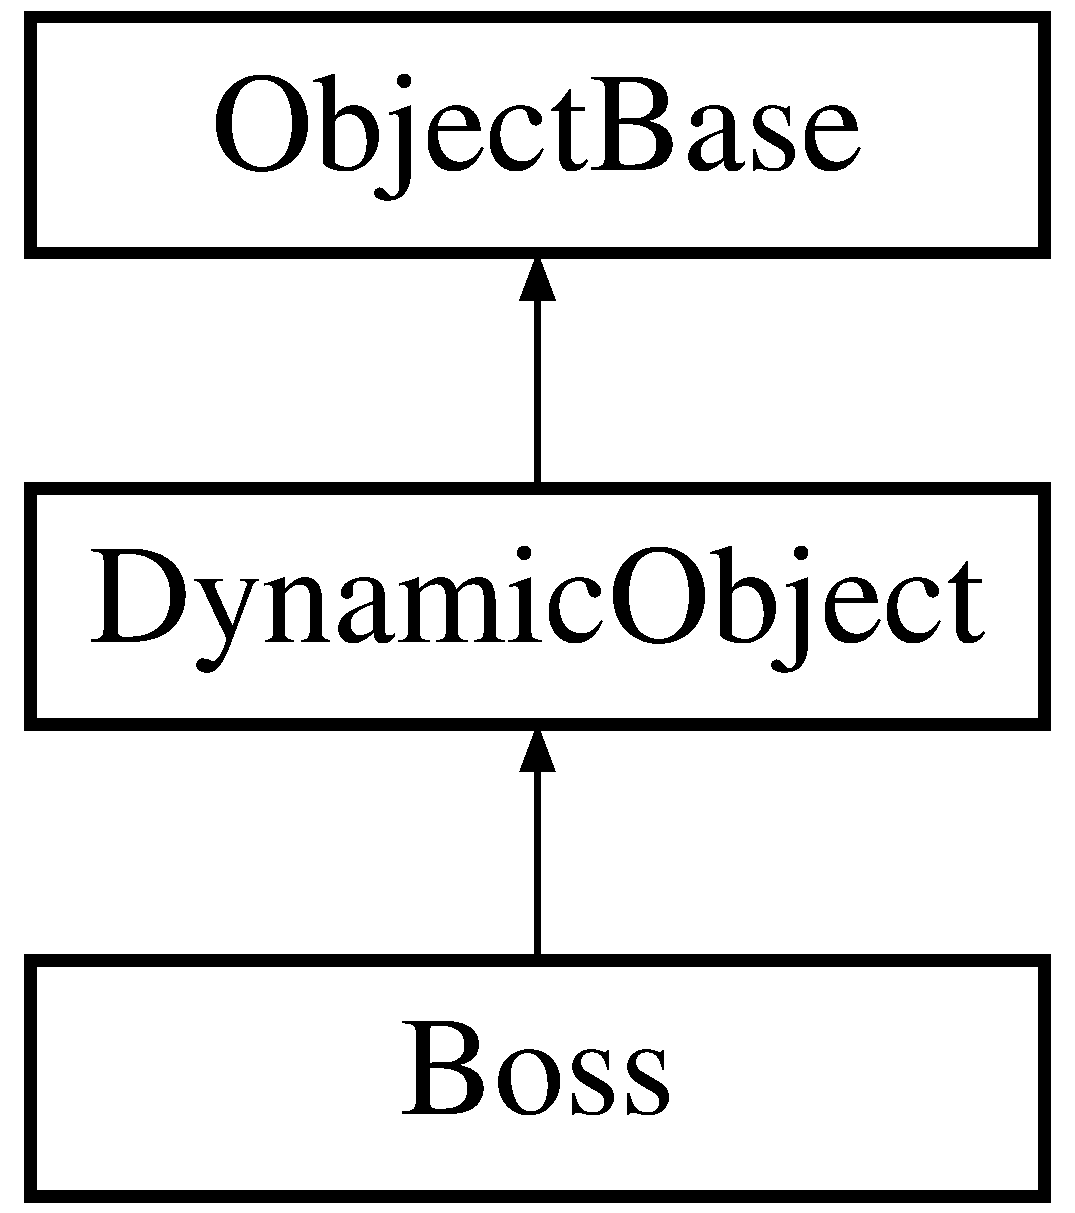
\includegraphics[height=3.000000cm]{class_boss}
\end{center}
\end{figure}
\subsection*{公開メンバ関数}
\begin{DoxyCompactItemize}
\item 
void \mbox{\hyperlink{class_boss_a3085cbf44a8e918abac0a62a6e443cab}{Set\+Max\+Hp}} (float max\+\_\+hp)
\item 
void \mbox{\hyperlink{class_boss_a417e06b76510146b1e6c0e6841e4463c}{Reset\+Speed}} ()
\item 
\mbox{\hyperlink{class_boss_af287739a9fe8cb9501795656d34f3018}{Boss}} ()
\begin{DoxyCompactList}\small\item\em コンストラクタ \end{DoxyCompactList}\item 
\mbox{\hyperlink{class_boss_ae6bb99cbbbb4a5ae7db4d174e6f4b50e}{Boss}} (const \mbox{\hyperlink{class_boss}{Boss}} \&ne)
\begin{DoxyCompactList}\small\item\em コピーコンストラクタ \end{DoxyCompactList}\item 
\mbox{\hyperlink{class_boss_a2e8bacd64a0212e890c62febaa37c988}{Boss}} (\mbox{\hyperlink{class_boss}{Boss}} \&\&ne) noexcept
\begin{DoxyCompactList}\small\item\em ムーブコンストラクタ \end{DoxyCompactList}\item 
\mbox{\hyperlink{class_boss}{Boss}} \& \mbox{\hyperlink{class_boss_ae84c6b0e64de86f606f5ac1348045371}{operator=}} (const \mbox{\hyperlink{class_boss}{Boss}} \&other)
\begin{DoxyCompactList}\small\item\em コピー代入演算子 \end{DoxyCompactList}\item 
void \mbox{\hyperlink{class_boss_a36b664185c0aa3ae4c6fc58c33d8485b}{Collision}} (\mbox{\hyperlink{class_object_base}{Object\+Base}} $\ast$, \mbox{\hyperlink{common_8h_ae148fff5818e9444b4ab2288829559bf}{Vec2}}) final
\begin{DoxyCompactList}\small\item\em エネミーの当たったときに実行する関数 \end{DoxyCompactList}\item 
void \mbox{\hyperlink{class_boss_afe7a503ea624c30c2a50b58b40acfb48}{Destroy}} () final
\begin{DoxyCompactList}\small\item\em エネミーの破棄 \end{DoxyCompactList}\item 
void \mbox{\hyperlink{class_boss_adb8591a0e2a919380e560f05b51fa171}{In\+Boss\+Scene}} (const float x)
\item 
void \mbox{\hyperlink{class_boss_a2d13fa10c0820f4131c145b6496a5e0b}{Translation\+Boss\+Scene}} ()
\item 
void \mbox{\hyperlink{class_boss_af1d3f76c28bff11d80530e4c8fdca355}{Destroy\+Ui}} ()
\item 
\mbox{\hyperlink{class_boss_ae2300fbed7e29873d66c5a89beb3a628}{$\sim$\+Boss}} ()
\begin{DoxyCompactList}\small\item\em デストラクタ \end{DoxyCompactList}\end{DoxyCompactItemize}
\subsection*{限定公開メンバ関数}
\begin{DoxyCompactItemize}
\item 
void \mbox{\hyperlink{class_boss_a460293079fd93f0ad2b98193fa367aa7}{Init\+Process}} () final
\begin{DoxyCompactList}\small\item\em エネミーの初期化 \end{DoxyCompactList}\item 
void \mbox{\hyperlink{class_boss_a12b3970fee863198d6dafb9bafc55d47}{Update\+Process}} () final
\begin{DoxyCompactList}\small\item\em エネミーの更新 \end{DoxyCompactList}\item 
void \mbox{\hyperlink{class_boss_a6681bd6fc6dc35e200f9e63f196301af}{Render\+Process}} (bool) final
\begin{DoxyCompactList}\small\item\em 描画 \end{DoxyCompactList}\end{DoxyCompactItemize}
\subsection*{その他の継承メンバ}


\subsection{構築子と解体子}
\mbox{\Hypertarget{class_boss_af287739a9fe8cb9501795656d34f3018}\label{class_boss_af287739a9fe8cb9501795656d34f3018}} 
\index{Boss@{Boss}!Boss@{Boss}}
\index{Boss@{Boss}!Boss@{Boss}}
\subsubsection{\texorpdfstring{Boss()}{Boss()}\hspace{0.1cm}{\footnotesize\ttfamily [1/3]}}
{\footnotesize\ttfamily Boss\+::\+Boss (\begin{DoxyParamCaption}{ }\end{DoxyParamCaption})\hspace{0.3cm}{\ttfamily [inline]}}



コンストラクタ 

\mbox{\Hypertarget{class_boss_ae6bb99cbbbb4a5ae7db4d174e6f4b50e}\label{class_boss_ae6bb99cbbbb4a5ae7db4d174e6f4b50e}} 
\index{Boss@{Boss}!Boss@{Boss}}
\index{Boss@{Boss}!Boss@{Boss}}
\subsubsection{\texorpdfstring{Boss()}{Boss()}\hspace{0.1cm}{\footnotesize\ttfamily [2/3]}}
{\footnotesize\ttfamily Boss\+::\+Boss (\begin{DoxyParamCaption}\item[{const \mbox{\hyperlink{class_boss}{Boss}} \&}]{ne }\end{DoxyParamCaption})\hspace{0.3cm}{\ttfamily [inline]}}



コピーコンストラクタ 

\mbox{\Hypertarget{class_boss_a2e8bacd64a0212e890c62febaa37c988}\label{class_boss_a2e8bacd64a0212e890c62febaa37c988}} 
\index{Boss@{Boss}!Boss@{Boss}}
\index{Boss@{Boss}!Boss@{Boss}}
\subsubsection{\texorpdfstring{Boss()}{Boss()}\hspace{0.1cm}{\footnotesize\ttfamily [3/3]}}
{\footnotesize\ttfamily Boss\+::\+Boss (\begin{DoxyParamCaption}\item[{\mbox{\hyperlink{class_boss}{Boss}} \&\&}]{ne }\end{DoxyParamCaption})\hspace{0.3cm}{\ttfamily [inline]}, {\ttfamily [noexcept]}}



ムーブコンストラクタ 

\mbox{\Hypertarget{class_boss_ae2300fbed7e29873d66c5a89beb3a628}\label{class_boss_ae2300fbed7e29873d66c5a89beb3a628}} 
\index{Boss@{Boss}!````~Boss@{$\sim$\+Boss}}
\index{````~Boss@{$\sim$\+Boss}!Boss@{Boss}}
\subsubsection{\texorpdfstring{$\sim$\+Boss()}{~Boss()}}
{\footnotesize\ttfamily Boss\+::$\sim$\+Boss (\begin{DoxyParamCaption}{ }\end{DoxyParamCaption})\hspace{0.3cm}{\ttfamily [inline]}}



デストラクタ 



\subsection{関数詳解}
\mbox{\Hypertarget{class_boss_a36b664185c0aa3ae4c6fc58c33d8485b}\label{class_boss_a36b664185c0aa3ae4c6fc58c33d8485b}} 
\index{Boss@{Boss}!Collision@{Collision}}
\index{Collision@{Collision}!Boss@{Boss}}
\subsubsection{\texorpdfstring{Collision()}{Collision()}}
{\footnotesize\ttfamily void Boss\+::\+Collision (\begin{DoxyParamCaption}\item[{\mbox{\hyperlink{class_object_base}{Object\+Base}} $\ast$}]{obj,  }\item[{\mbox{\hyperlink{common_8h_ae148fff5818e9444b4ab2288829559bf}{Vec2}}}]{ }\end{DoxyParamCaption})\hspace{0.3cm}{\ttfamily [final]}, {\ttfamily [virtual]}}



エネミーの当たったときに実行する関数 


\begin{DoxyParams}{引数}
{\em obj 当たった相手のオブジェクト} & \\
\hline
\end{DoxyParams}


\mbox{\hyperlink{class_object_base_a3e1db79dfa119be067d816c22d09839d}{Object\+Base}}を再実装しています。

\mbox{\Hypertarget{class_boss_afe7a503ea624c30c2a50b58b40acfb48}\label{class_boss_afe7a503ea624c30c2a50b58b40acfb48}} 
\index{Boss@{Boss}!Destroy@{Destroy}}
\index{Destroy@{Destroy}!Boss@{Boss}}
\subsubsection{\texorpdfstring{Destroy()}{Destroy()}}
{\footnotesize\ttfamily void Boss\+::\+Destroy (\begin{DoxyParamCaption}{ }\end{DoxyParamCaption})\hspace{0.3cm}{\ttfamily [final]}, {\ttfamily [virtual]}}



エネミーの破棄 



\mbox{\hyperlink{class_object_base_a7fa4c548153c3af20f89673ffea809af}{Object\+Base}}を実装しています。

\mbox{\Hypertarget{class_boss_af1d3f76c28bff11d80530e4c8fdca355}\label{class_boss_af1d3f76c28bff11d80530e4c8fdca355}} 
\index{Boss@{Boss}!Destroy\+Ui@{Destroy\+Ui}}
\index{Destroy\+Ui@{Destroy\+Ui}!Boss@{Boss}}
\subsubsection{\texorpdfstring{Destroy\+Ui()}{DestroyUi()}}
{\footnotesize\ttfamily void Boss\+::\+Destroy\+Ui (\begin{DoxyParamCaption}{ }\end{DoxyParamCaption})\hspace{0.3cm}{\ttfamily [inline]}}

\mbox{\Hypertarget{class_boss_adb8591a0e2a919380e560f05b51fa171}\label{class_boss_adb8591a0e2a919380e560f05b51fa171}} 
\index{Boss@{Boss}!In\+Boss\+Scene@{In\+Boss\+Scene}}
\index{In\+Boss\+Scene@{In\+Boss\+Scene}!Boss@{Boss}}
\subsubsection{\texorpdfstring{In\+Boss\+Scene()}{InBossScene()}}
{\footnotesize\ttfamily void Boss\+::\+In\+Boss\+Scene (\begin{DoxyParamCaption}\item[{const float}]{x }\end{DoxyParamCaption})\hspace{0.3cm}{\ttfamily [inline]}}

\mbox{\Hypertarget{class_boss_a460293079fd93f0ad2b98193fa367aa7}\label{class_boss_a460293079fd93f0ad2b98193fa367aa7}} 
\index{Boss@{Boss}!Init\+Process@{Init\+Process}}
\index{Init\+Process@{Init\+Process}!Boss@{Boss}}
\subsubsection{\texorpdfstring{Init\+Process()}{InitProcess()}}
{\footnotesize\ttfamily void Boss\+::\+Init\+Process (\begin{DoxyParamCaption}{ }\end{DoxyParamCaption})\hspace{0.3cm}{\ttfamily [final]}, {\ttfamily [protected]}, {\ttfamily [virtual]}}



エネミーの初期化 



\mbox{\hyperlink{class_object_base_af133f36f2bca1dcfd962e2cfac61ab51}{Object\+Base}}を実装しています。

\mbox{\Hypertarget{class_boss_ae84c6b0e64de86f606f5ac1348045371}\label{class_boss_ae84c6b0e64de86f606f5ac1348045371}} 
\index{Boss@{Boss}!operator=@{operator=}}
\index{operator=@{operator=}!Boss@{Boss}}
\subsubsection{\texorpdfstring{operator=()}{operator=()}}
{\footnotesize\ttfamily \mbox{\hyperlink{class_boss}{Boss}}\& Boss\+::operator= (\begin{DoxyParamCaption}\item[{const \mbox{\hyperlink{class_boss}{Boss}} \&}]{other }\end{DoxyParamCaption})\hspace{0.3cm}{\ttfamily [inline]}}



コピー代入演算子 

\mbox{\Hypertarget{class_boss_a6681bd6fc6dc35e200f9e63f196301af}\label{class_boss_a6681bd6fc6dc35e200f9e63f196301af}} 
\index{Boss@{Boss}!Render\+Process@{Render\+Process}}
\index{Render\+Process@{Render\+Process}!Boss@{Boss}}
\subsubsection{\texorpdfstring{Render\+Process()}{RenderProcess()}}
{\footnotesize\ttfamily void Boss\+::\+Render\+Process (\begin{DoxyParamCaption}\item[{bool}]{camera\+\_\+affected }\end{DoxyParamCaption})\hspace{0.3cm}{\ttfamily [final]}, {\ttfamily [protected]}, {\ttfamily [virtual]}}



描画 


\begin{DoxyParams}{引数}
{\em camera\+\_\+affected} & カメラの位置によって位置を変えるかどうか \\
\hline
\end{DoxyParams}


\mbox{\hyperlink{class_dynamic_object_aa7488e1b4dfd7049447535d93d9d6783}{Dynamic\+Object}}を再実装しています。

\mbox{\Hypertarget{class_boss_a417e06b76510146b1e6c0e6841e4463c}\label{class_boss_a417e06b76510146b1e6c0e6841e4463c}} 
\index{Boss@{Boss}!Reset\+Speed@{Reset\+Speed}}
\index{Reset\+Speed@{Reset\+Speed}!Boss@{Boss}}
\subsubsection{\texorpdfstring{Reset\+Speed()}{ResetSpeed()}}
{\footnotesize\ttfamily void Boss\+::\+Reset\+Speed (\begin{DoxyParamCaption}{ }\end{DoxyParamCaption})\hspace{0.3cm}{\ttfamily [inline]}}

\mbox{\Hypertarget{class_boss_a3085cbf44a8e918abac0a62a6e443cab}\label{class_boss_a3085cbf44a8e918abac0a62a6e443cab}} 
\index{Boss@{Boss}!Set\+Max\+Hp@{Set\+Max\+Hp}}
\index{Set\+Max\+Hp@{Set\+Max\+Hp}!Boss@{Boss}}
\subsubsection{\texorpdfstring{Set\+Max\+Hp()}{SetMaxHp()}}
{\footnotesize\ttfamily void Boss\+::\+Set\+Max\+Hp (\begin{DoxyParamCaption}\item[{float}]{max\+\_\+hp }\end{DoxyParamCaption})\hspace{0.3cm}{\ttfamily [inline]}}

\mbox{\Hypertarget{class_boss_a2d13fa10c0820f4131c145b6496a5e0b}\label{class_boss_a2d13fa10c0820f4131c145b6496a5e0b}} 
\index{Boss@{Boss}!Translation\+Boss\+Scene@{Translation\+Boss\+Scene}}
\index{Translation\+Boss\+Scene@{Translation\+Boss\+Scene}!Boss@{Boss}}
\subsubsection{\texorpdfstring{Translation\+Boss\+Scene()}{TranslationBossScene()}}
{\footnotesize\ttfamily void Boss\+::\+Translation\+Boss\+Scene (\begin{DoxyParamCaption}{ }\end{DoxyParamCaption})\hspace{0.3cm}{\ttfamily [inline]}}

\mbox{\Hypertarget{class_boss_a12b3970fee863198d6dafb9bafc55d47}\label{class_boss_a12b3970fee863198d6dafb9bafc55d47}} 
\index{Boss@{Boss}!Update\+Process@{Update\+Process}}
\index{Update\+Process@{Update\+Process}!Boss@{Boss}}
\subsubsection{\texorpdfstring{Update\+Process()}{UpdateProcess()}}
{\footnotesize\ttfamily void Boss\+::\+Update\+Process (\begin{DoxyParamCaption}{ }\end{DoxyParamCaption})\hspace{0.3cm}{\ttfamily [final]}, {\ttfamily [protected]}, {\ttfamily [virtual]}}



エネミーの更新 



\mbox{\hyperlink{class_object_base_a8b5b72b363a419767efde0b0e692ea95}{Object\+Base}}を実装しています。



このクラス詳解は次のファイルから抽出されました\+:\begin{DoxyCompactItemize}
\item 
C\+:/\+Users/tokir/\+Documents/\+Git\+Hub/\+Weapon\+Merchant\+Adventure/src/src/object/character/enemy/boss/\mbox{\hyperlink{boss_8h}{boss.\+h}}\item 
C\+:/\+Users/tokir/\+Documents/\+Git\+Hub/\+Weapon\+Merchant\+Adventure/src/src/object/character/enemy/boss/\mbox{\hyperlink{boss_8cpp}{boss.\+cpp}}\end{DoxyCompactItemize}

\hypertarget{class_boss_bullet}{}\section{Boss\+Bullet クラス}
\label{class_boss_bullet}\index{Boss\+Bullet@{Boss\+Bullet}}


{\ttfamily \#include $<$boss\+\_\+bullet.\+h$>$}

Boss\+Bullet の継承関係図\begin{figure}[H]
\begin{center}
\leavevmode
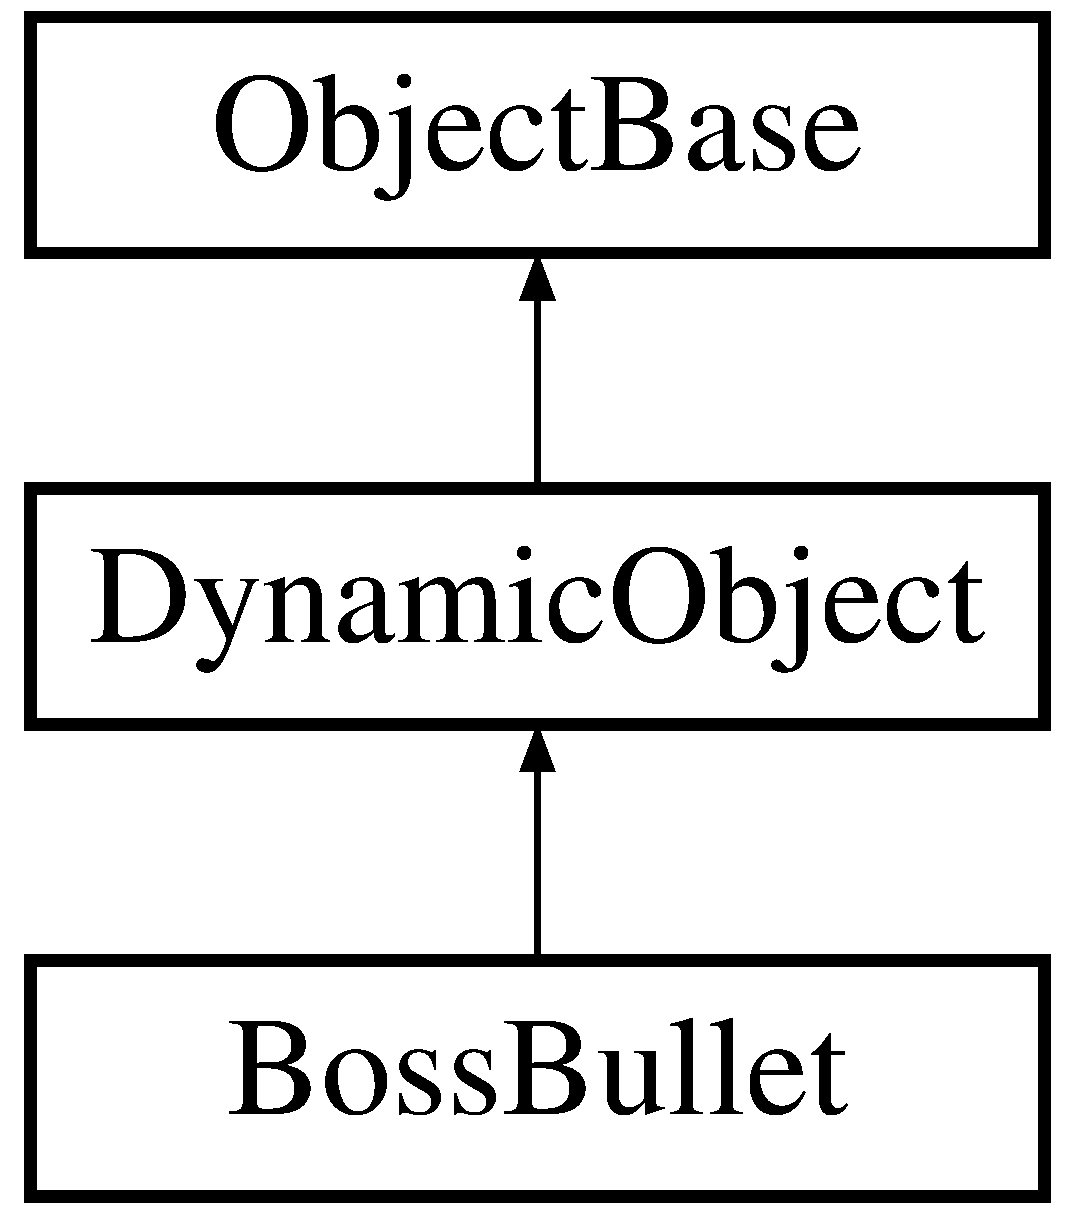
\includegraphics[height=3.000000cm]{class_boss_bullet}
\end{center}
\end{figure}
\subsection*{公開メンバ関数}
\begin{DoxyCompactItemize}
\item 
void \mbox{\hyperlink{class_boss_bullet_a29bc4989a8b16a9da0daa3da92fb0e0a}{Set\+Vector}} (const \mbox{\hyperlink{common_8h_ae148fff5818e9444b4ab2288829559bf}{Vec2}} vec2)
\item 
void \mbox{\hyperlink{class_boss_bullet_ace134e26eed55f3a839b8c6412664234}{Destroy}} () final
\item 
\mbox{\hyperlink{class_boss_bullet_acca8ecca1f90ed4454ca2bb3f20a86f9}{Boss\+Bullet}} ()
\item 
\mbox{\hyperlink{class_boss_bullet_a3fc4ad096e796b25d28e19ae8e4339bf}{Boss\+Bullet}} (const \mbox{\hyperlink{class_boss_bullet}{Boss\+Bullet}} \&other)
\item 
\mbox{\hyperlink{class_boss_bullet}{Boss\+Bullet}} \& \mbox{\hyperlink{class_boss_bullet_ab71ff0c91873433ba21e912c85800e1e}{operator=}} (const \mbox{\hyperlink{class_boss_bullet}{Boss\+Bullet}} \&other)
\begin{DoxyCompactList}\small\item\em コピー代入演算子 \end{DoxyCompactList}\item 
\mbox{\hyperlink{class_boss_bullet_a852db4124cf1985c9bb612ef8a765722}{Boss\+Bullet}} (\mbox{\hyperlink{class_boss_bullet}{Boss\+Bullet}} \&\&other)
\begin{DoxyCompactList}\small\item\em ムーブコンストラクタ \end{DoxyCompactList}\item 
void \mbox{\hyperlink{class_boss_bullet_ab742fa1d233e0df5d49cc239e24eeec3}{Collision}} (\mbox{\hyperlink{class_object_base}{Object\+Base}} $\ast$, \mbox{\hyperlink{common_8h_ae148fff5818e9444b4ab2288829559bf}{Vec2}}) final
\begin{DoxyCompactList}\small\item\em 当たってるときに実行する関数 \end{DoxyCompactList}\item 
\mbox{\hyperlink{class_boss_bullet_a387327aee4bbfba8abd6320f6f5acb35}{$\sim$\+Boss\+Bullet}} ()
\end{DoxyCompactItemize}
\subsection*{限定公開メンバ関数}
\begin{DoxyCompactItemize}
\item 
void \mbox{\hyperlink{class_boss_bullet_a8d70eb5a70dcf3d09baf646ae1bcb7f7}{Init\+Process}} () final
\item 
void \mbox{\hyperlink{class_boss_bullet_a8e9923194c03eb0d4225ed8dae409f29}{Update\+Process}} () final
\end{DoxyCompactItemize}
\subsection*{その他の継承メンバ}


\subsection{構築子と解体子}
\mbox{\Hypertarget{class_boss_bullet_acca8ecca1f90ed4454ca2bb3f20a86f9}\label{class_boss_bullet_acca8ecca1f90ed4454ca2bb3f20a86f9}} 
\index{Boss\+Bullet@{Boss\+Bullet}!Boss\+Bullet@{Boss\+Bullet}}
\index{Boss\+Bullet@{Boss\+Bullet}!Boss\+Bullet@{Boss\+Bullet}}
\subsubsection{\texorpdfstring{Boss\+Bullet()}{BossBullet()}\hspace{0.1cm}{\footnotesize\ttfamily [1/3]}}
{\footnotesize\ttfamily Boss\+Bullet\+::\+Boss\+Bullet (\begin{DoxyParamCaption}{ }\end{DoxyParamCaption})\hspace{0.3cm}{\ttfamily [inline]}}

\mbox{\Hypertarget{class_boss_bullet_a3fc4ad096e796b25d28e19ae8e4339bf}\label{class_boss_bullet_a3fc4ad096e796b25d28e19ae8e4339bf}} 
\index{Boss\+Bullet@{Boss\+Bullet}!Boss\+Bullet@{Boss\+Bullet}}
\index{Boss\+Bullet@{Boss\+Bullet}!Boss\+Bullet@{Boss\+Bullet}}
\subsubsection{\texorpdfstring{Boss\+Bullet()}{BossBullet()}\hspace{0.1cm}{\footnotesize\ttfamily [2/3]}}
{\footnotesize\ttfamily Boss\+Bullet\+::\+Boss\+Bullet (\begin{DoxyParamCaption}\item[{const \mbox{\hyperlink{class_boss_bullet}{Boss\+Bullet}} \&}]{other }\end{DoxyParamCaption})\hspace{0.3cm}{\ttfamily [inline]}}

\mbox{\Hypertarget{class_boss_bullet_a852db4124cf1985c9bb612ef8a765722}\label{class_boss_bullet_a852db4124cf1985c9bb612ef8a765722}} 
\index{Boss\+Bullet@{Boss\+Bullet}!Boss\+Bullet@{Boss\+Bullet}}
\index{Boss\+Bullet@{Boss\+Bullet}!Boss\+Bullet@{Boss\+Bullet}}
\subsubsection{\texorpdfstring{Boss\+Bullet()}{BossBullet()}\hspace{0.1cm}{\footnotesize\ttfamily [3/3]}}
{\footnotesize\ttfamily Boss\+Bullet\+::\+Boss\+Bullet (\begin{DoxyParamCaption}\item[{\mbox{\hyperlink{class_boss_bullet}{Boss\+Bullet}} \&\&}]{other }\end{DoxyParamCaption})\hspace{0.3cm}{\ttfamily [inline]}}



ムーブコンストラクタ 

\mbox{\Hypertarget{class_boss_bullet_a387327aee4bbfba8abd6320f6f5acb35}\label{class_boss_bullet_a387327aee4bbfba8abd6320f6f5acb35}} 
\index{Boss\+Bullet@{Boss\+Bullet}!````~Boss\+Bullet@{$\sim$\+Boss\+Bullet}}
\index{````~Boss\+Bullet@{$\sim$\+Boss\+Bullet}!Boss\+Bullet@{Boss\+Bullet}}
\subsubsection{\texorpdfstring{$\sim$\+Boss\+Bullet()}{~BossBullet()}}
{\footnotesize\ttfamily Boss\+Bullet\+::$\sim$\+Boss\+Bullet (\begin{DoxyParamCaption}{ }\end{DoxyParamCaption})\hspace{0.3cm}{\ttfamily [inline]}}



\subsection{関数詳解}
\mbox{\Hypertarget{class_boss_bullet_ab742fa1d233e0df5d49cc239e24eeec3}\label{class_boss_bullet_ab742fa1d233e0df5d49cc239e24eeec3}} 
\index{Boss\+Bullet@{Boss\+Bullet}!Collision@{Collision}}
\index{Collision@{Collision}!Boss\+Bullet@{Boss\+Bullet}}
\subsubsection{\texorpdfstring{Collision()}{Collision()}}
{\footnotesize\ttfamily void Boss\+Bullet\+::\+Collision (\begin{DoxyParamCaption}\item[{\mbox{\hyperlink{class_object_base}{Object\+Base}} $\ast$}]{obj,  }\item[{\mbox{\hyperlink{common_8h_ae148fff5818e9444b4ab2288829559bf}{Vec2}}}]{ }\end{DoxyParamCaption})\hspace{0.3cm}{\ttfamily [final]}, {\ttfamily [virtual]}}



当たってるときに実行する関数 



\mbox{\hyperlink{class_object_base_a3e1db79dfa119be067d816c22d09839d}{Object\+Base}}を再実装しています。

\mbox{\Hypertarget{class_boss_bullet_ace134e26eed55f3a839b8c6412664234}\label{class_boss_bullet_ace134e26eed55f3a839b8c6412664234}} 
\index{Boss\+Bullet@{Boss\+Bullet}!Destroy@{Destroy}}
\index{Destroy@{Destroy}!Boss\+Bullet@{Boss\+Bullet}}
\subsubsection{\texorpdfstring{Destroy()}{Destroy()}}
{\footnotesize\ttfamily void Boss\+Bullet\+::\+Destroy (\begin{DoxyParamCaption}{ }\end{DoxyParamCaption})\hspace{0.3cm}{\ttfamily [final]}, {\ttfamily [virtual]}}



\mbox{\hyperlink{class_object_base_a7fa4c548153c3af20f89673ffea809af}{Object\+Base}}を実装しています。

\mbox{\Hypertarget{class_boss_bullet_a8d70eb5a70dcf3d09baf646ae1bcb7f7}\label{class_boss_bullet_a8d70eb5a70dcf3d09baf646ae1bcb7f7}} 
\index{Boss\+Bullet@{Boss\+Bullet}!Init\+Process@{Init\+Process}}
\index{Init\+Process@{Init\+Process}!Boss\+Bullet@{Boss\+Bullet}}
\subsubsection{\texorpdfstring{Init\+Process()}{InitProcess()}}
{\footnotesize\ttfamily void Boss\+Bullet\+::\+Init\+Process (\begin{DoxyParamCaption}{ }\end{DoxyParamCaption})\hspace{0.3cm}{\ttfamily [final]}, {\ttfamily [protected]}, {\ttfamily [virtual]}}



\mbox{\hyperlink{class_object_base_af133f36f2bca1dcfd962e2cfac61ab51}{Object\+Base}}を実装しています。

\mbox{\Hypertarget{class_boss_bullet_ab71ff0c91873433ba21e912c85800e1e}\label{class_boss_bullet_ab71ff0c91873433ba21e912c85800e1e}} 
\index{Boss\+Bullet@{Boss\+Bullet}!operator=@{operator=}}
\index{operator=@{operator=}!Boss\+Bullet@{Boss\+Bullet}}
\subsubsection{\texorpdfstring{operator=()}{operator=()}}
{\footnotesize\ttfamily \mbox{\hyperlink{class_boss_bullet}{Boss\+Bullet}}\& Boss\+Bullet\+::operator= (\begin{DoxyParamCaption}\item[{const \mbox{\hyperlink{class_boss_bullet}{Boss\+Bullet}} \&}]{other }\end{DoxyParamCaption})\hspace{0.3cm}{\ttfamily [inline]}}



コピー代入演算子 

\mbox{\Hypertarget{class_boss_bullet_a29bc4989a8b16a9da0daa3da92fb0e0a}\label{class_boss_bullet_a29bc4989a8b16a9da0daa3da92fb0e0a}} 
\index{Boss\+Bullet@{Boss\+Bullet}!Set\+Vector@{Set\+Vector}}
\index{Set\+Vector@{Set\+Vector}!Boss\+Bullet@{Boss\+Bullet}}
\subsubsection{\texorpdfstring{Set\+Vector()}{SetVector()}}
{\footnotesize\ttfamily void Boss\+Bullet\+::\+Set\+Vector (\begin{DoxyParamCaption}\item[{const \mbox{\hyperlink{common_8h_ae148fff5818e9444b4ab2288829559bf}{Vec2}}}]{vec2 }\end{DoxyParamCaption})\hspace{0.3cm}{\ttfamily [inline]}}

\mbox{\Hypertarget{class_boss_bullet_a8e9923194c03eb0d4225ed8dae409f29}\label{class_boss_bullet_a8e9923194c03eb0d4225ed8dae409f29}} 
\index{Boss\+Bullet@{Boss\+Bullet}!Update\+Process@{Update\+Process}}
\index{Update\+Process@{Update\+Process}!Boss\+Bullet@{Boss\+Bullet}}
\subsubsection{\texorpdfstring{Update\+Process()}{UpdateProcess()}}
{\footnotesize\ttfamily void Boss\+Bullet\+::\+Update\+Process (\begin{DoxyParamCaption}{ }\end{DoxyParamCaption})\hspace{0.3cm}{\ttfamily [final]}, {\ttfamily [protected]}, {\ttfamily [virtual]}}



\mbox{\hyperlink{class_object_base_a8b5b72b363a419767efde0b0e692ea95}{Object\+Base}}を実装しています。



このクラス詳解は次のファイルから抽出されました\+:\begin{DoxyCompactItemize}
\item 
C\+:/\+Users/tokir/\+Documents/\+Git\+Hub/\+Weapon\+Merchant\+Adventure/src/src/object/character/enemy/boss/action\+\_\+pattern/attack/bullet/\mbox{\hyperlink{boss__bullet_8h}{boss\+\_\+bullet.\+h}}\item 
C\+:/\+Users/tokir/\+Documents/\+Git\+Hub/\+Weapon\+Merchant\+Adventure/src/src/object/character/enemy/boss/action\+\_\+pattern/attack/bullet/\mbox{\hyperlink{boss__bullet_8cpp}{boss\+\_\+bullet.\+cpp}}\end{DoxyCompactItemize}

\hypertarget{class_bullet}{}\section{Bullet クラス}
\label{class_bullet}\index{Bullet@{Bullet}}


弾クラス  




{\ttfamily \#include $<$bullet.\+h$>$}

Bullet の継承関係図\begin{figure}[H]
\begin{center}
\leavevmode
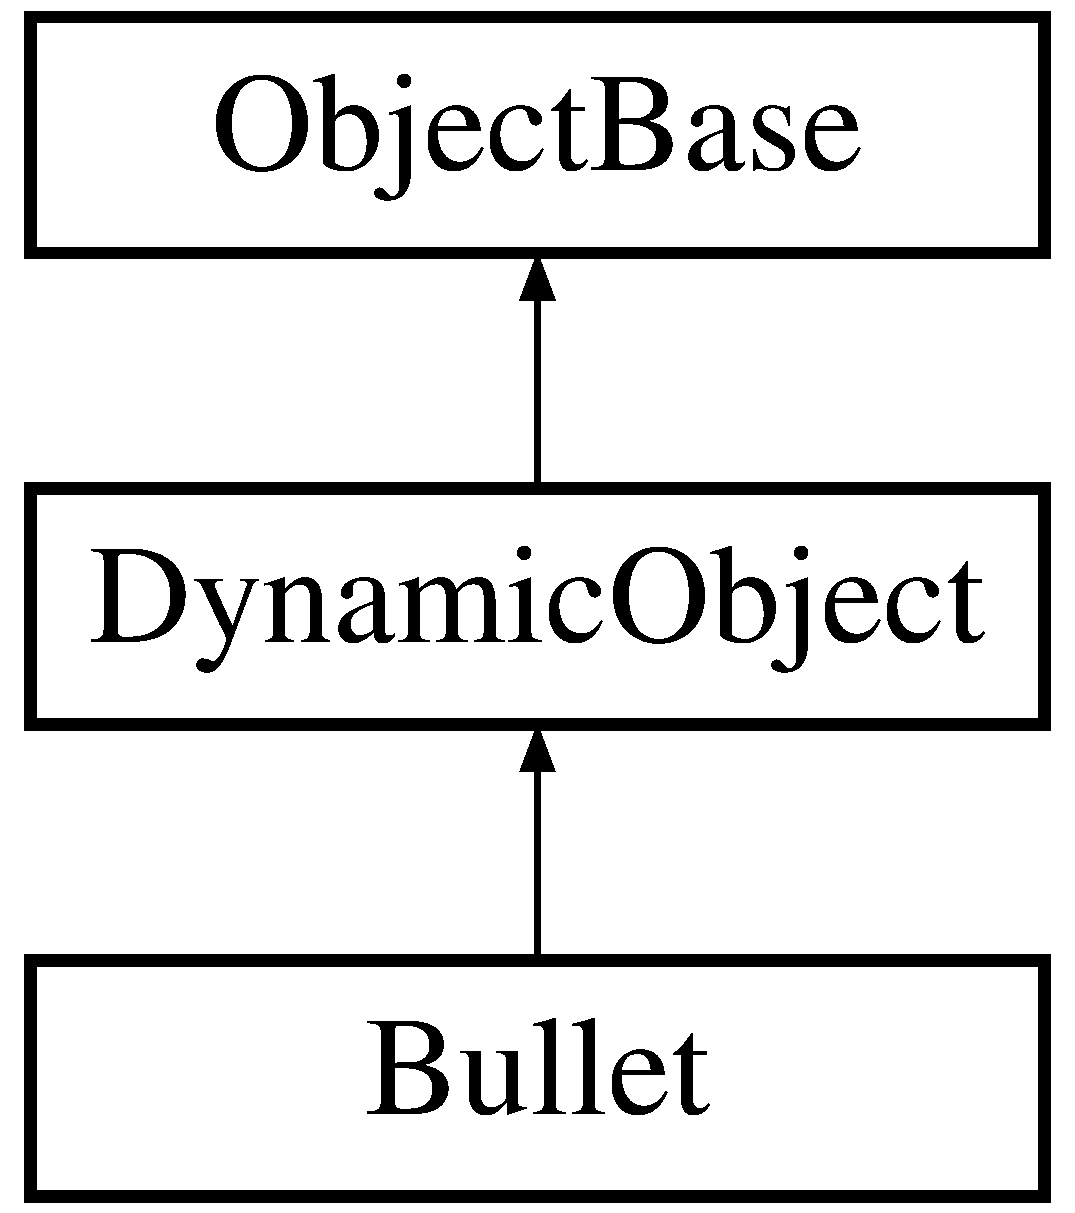
\includegraphics[height=3.000000cm]{class_bullet}
\end{center}
\end{figure}
\subsection*{公開メンバ関数}
\begin{DoxyCompactItemize}
\item 
\mbox{\hyperlink{class_bullet_acd7befc0bc18907cc1d871d37bbdddeb}{Bullet}} ()
\begin{DoxyCompactList}\small\item\em コンストラクタ \end{DoxyCompactList}\item 
\mbox{\hyperlink{class_bullet_a7e1ed7ba89e019b3d0fd068cfb4f9a6d}{Bullet}} (const \mbox{\hyperlink{class_bullet}{Bullet}} \&b)
\begin{DoxyCompactList}\small\item\em コピーコンストラクタ \end{DoxyCompactList}\item 
\mbox{\hyperlink{class_bullet}{Bullet}} \& \mbox{\hyperlink{class_bullet_a2a98443028be8389c0eb9da9a09f661c}{operator=}} (const \mbox{\hyperlink{class_bullet}{Bullet}} \&other)
\begin{DoxyCompactList}\small\item\em コピー代入演算子 \end{DoxyCompactList}\item 
\mbox{\hyperlink{class_bullet_a4bf8f227cde57a6abcdd268df2ef9a9d}{Bullet}} (\mbox{\hyperlink{class_bullet}{Bullet}} \&\&b)
\begin{DoxyCompactList}\small\item\em ムーブコンストラクタ \end{DoxyCompactList}\item 
void \mbox{\hyperlink{class_bullet_ab6b7b4ebc19095372a8e5ef3ad45ff65}{Bullet\+Init}} (const float, const std\+::function$<$ void()$>$ \&)
\begin{DoxyCompactList}\small\item\em 弾の初期化 \end{DoxyCompactList}\item 
void \mbox{\hyperlink{class_bullet_a09a92c6b924fb6bc38e18f6c41ac20ff}{Destroy}} () final
\begin{DoxyCompactList}\small\item\em 破棄 \end{DoxyCompactList}\item 
void \mbox{\hyperlink{class_bullet_a945da4a16d11cfee31139d564bea61f0}{Collision}} (\mbox{\hyperlink{class_object_base}{Object\+Base}} $\ast$, \mbox{\hyperlink{common_8h_afb0c5e21d4133ff4f200992c0b534e1b}{V\+E\+C2}}) final
\begin{DoxyCompactList}\small\item\em 当たったときに実行する関数 \end{DoxyCompactList}\item 
\mbox{\hyperlink{class_bullet_aaeb5cb41d7db89f49007b08b41f1bfcf}{$\sim$\+Bullet}} ()
\begin{DoxyCompactList}\small\item\em デストラクタ \end{DoxyCompactList}\end{DoxyCompactItemize}
\subsection*{限定公開メンバ関数}
\begin{DoxyCompactItemize}
\item 
void \mbox{\hyperlink{class_bullet_a448c1c566e002d7b51ba6ed5c927bff7}{Init\+Process}} () final
\begin{DoxyCompactList}\small\item\em 初期化 \end{DoxyCompactList}\item 
void \mbox{\hyperlink{class_bullet_aa0867038c9c35e30ee09e21ecdccf281}{Update\+Process}} () final
\begin{DoxyCompactList}\small\item\em 更新 \end{DoxyCompactList}\end{DoxyCompactItemize}
\subsection*{その他の継承メンバ}


\subsection{詳解}
弾クラス 

\subsection{構築子と解体子}
\mbox{\Hypertarget{class_bullet_acd7befc0bc18907cc1d871d37bbdddeb}\label{class_bullet_acd7befc0bc18907cc1d871d37bbdddeb}} 
\index{Bullet@{Bullet}!Bullet@{Bullet}}
\index{Bullet@{Bullet}!Bullet@{Bullet}}
\subsubsection{\texorpdfstring{Bullet()}{Bullet()}\hspace{0.1cm}{\footnotesize\ttfamily [1/3]}}
{\footnotesize\ttfamily Bullet\+::\+Bullet (\begin{DoxyParamCaption}{ }\end{DoxyParamCaption})\hspace{0.3cm}{\ttfamily [inline]}}



コンストラクタ 

\mbox{\Hypertarget{class_bullet_a7e1ed7ba89e019b3d0fd068cfb4f9a6d}\label{class_bullet_a7e1ed7ba89e019b3d0fd068cfb4f9a6d}} 
\index{Bullet@{Bullet}!Bullet@{Bullet}}
\index{Bullet@{Bullet}!Bullet@{Bullet}}
\subsubsection{\texorpdfstring{Bullet()}{Bullet()}\hspace{0.1cm}{\footnotesize\ttfamily [2/3]}}
{\footnotesize\ttfamily Bullet\+::\+Bullet (\begin{DoxyParamCaption}\item[{const \mbox{\hyperlink{class_bullet}{Bullet}} \&}]{b }\end{DoxyParamCaption})\hspace{0.3cm}{\ttfamily [inline]}}



コピーコンストラクタ 

\mbox{\Hypertarget{class_bullet_a4bf8f227cde57a6abcdd268df2ef9a9d}\label{class_bullet_a4bf8f227cde57a6abcdd268df2ef9a9d}} 
\index{Bullet@{Bullet}!Bullet@{Bullet}}
\index{Bullet@{Bullet}!Bullet@{Bullet}}
\subsubsection{\texorpdfstring{Bullet()}{Bullet()}\hspace{0.1cm}{\footnotesize\ttfamily [3/3]}}
{\footnotesize\ttfamily Bullet\+::\+Bullet (\begin{DoxyParamCaption}\item[{\mbox{\hyperlink{class_bullet}{Bullet}} \&\&}]{b }\end{DoxyParamCaption})\hspace{0.3cm}{\ttfamily [inline]}}



ムーブコンストラクタ 

\mbox{\Hypertarget{class_bullet_aaeb5cb41d7db89f49007b08b41f1bfcf}\label{class_bullet_aaeb5cb41d7db89f49007b08b41f1bfcf}} 
\index{Bullet@{Bullet}!````~Bullet@{$\sim$\+Bullet}}
\index{````~Bullet@{$\sim$\+Bullet}!Bullet@{Bullet}}
\subsubsection{\texorpdfstring{$\sim$\+Bullet()}{~Bullet()}}
{\footnotesize\ttfamily Bullet\+::$\sim$\+Bullet (\begin{DoxyParamCaption}{ }\end{DoxyParamCaption})\hspace{0.3cm}{\ttfamily [inline]}}



デストラクタ 



\subsection{関数詳解}
\mbox{\Hypertarget{class_bullet_ab6b7b4ebc19095372a8e5ef3ad45ff65}\label{class_bullet_ab6b7b4ebc19095372a8e5ef3ad45ff65}} 
\index{Bullet@{Bullet}!Bullet\+Init@{Bullet\+Init}}
\index{Bullet\+Init@{Bullet\+Init}!Bullet@{Bullet}}
\subsubsection{\texorpdfstring{Bullet\+Init()}{BulletInit()}}
{\footnotesize\ttfamily void Bullet\+::\+Bullet\+Init (\begin{DoxyParamCaption}\item[{const float}]{angle,  }\item[{const std\+::function$<$ void()$>$ \&}]{func }\end{DoxyParamCaption})}



弾の初期化 


\begin{DoxyParams}{引数}
{\em angle} & 発射角度 \\
\hline
{\em func} & 当たったときに実行する関数 \\
\hline
\end{DoxyParams}
\mbox{\Hypertarget{class_bullet_a945da4a16d11cfee31139d564bea61f0}\label{class_bullet_a945da4a16d11cfee31139d564bea61f0}} 
\index{Bullet@{Bullet}!Collision@{Collision}}
\index{Collision@{Collision}!Bullet@{Bullet}}
\subsubsection{\texorpdfstring{Collision()}{Collision()}}
{\footnotesize\ttfamily void Bullet\+::\+Collision (\begin{DoxyParamCaption}\item[{\mbox{\hyperlink{class_object_base}{Object\+Base}} $\ast$}]{obj,  }\item[{\mbox{\hyperlink{common_8h_afb0c5e21d4133ff4f200992c0b534e1b}{V\+E\+C2}}}]{ }\end{DoxyParamCaption})\hspace{0.3cm}{\ttfamily [final]}, {\ttfamily [virtual]}}



当たったときに実行する関数 


\begin{DoxyParams}{引数}
{\em obj} & 当たった相手のオブジェクト \\
\hline
\end{DoxyParams}


\mbox{\hyperlink{class_object_base_ad772d7a42f5e46c39481f5db22ee8193}{Object\+Base}}を再実装しています。

\mbox{\Hypertarget{class_bullet_a09a92c6b924fb6bc38e18f6c41ac20ff}\label{class_bullet_a09a92c6b924fb6bc38e18f6c41ac20ff}} 
\index{Bullet@{Bullet}!Destroy@{Destroy}}
\index{Destroy@{Destroy}!Bullet@{Bullet}}
\subsubsection{\texorpdfstring{Destroy()}{Destroy()}}
{\footnotesize\ttfamily void Bullet\+::\+Destroy (\begin{DoxyParamCaption}{ }\end{DoxyParamCaption})\hspace{0.3cm}{\ttfamily [final]}, {\ttfamily [virtual]}}



破棄 



\mbox{\hyperlink{class_object_base_a7fa4c548153c3af20f89673ffea809af}{Object\+Base}}を実装しています。

\mbox{\Hypertarget{class_bullet_a448c1c566e002d7b51ba6ed5c927bff7}\label{class_bullet_a448c1c566e002d7b51ba6ed5c927bff7}} 
\index{Bullet@{Bullet}!Init\+Process@{Init\+Process}}
\index{Init\+Process@{Init\+Process}!Bullet@{Bullet}}
\subsubsection{\texorpdfstring{Init\+Process()}{InitProcess()}}
{\footnotesize\ttfamily void Bullet\+::\+Init\+Process (\begin{DoxyParamCaption}{ }\end{DoxyParamCaption})\hspace{0.3cm}{\ttfamily [final]}, {\ttfamily [protected]}, {\ttfamily [virtual]}}



初期化 



\mbox{\hyperlink{class_object_base_af133f36f2bca1dcfd962e2cfac61ab51}{Object\+Base}}を実装しています。

\mbox{\Hypertarget{class_bullet_a2a98443028be8389c0eb9da9a09f661c}\label{class_bullet_a2a98443028be8389c0eb9da9a09f661c}} 
\index{Bullet@{Bullet}!operator=@{operator=}}
\index{operator=@{operator=}!Bullet@{Bullet}}
\subsubsection{\texorpdfstring{operator=()}{operator=()}}
{\footnotesize\ttfamily \mbox{\hyperlink{class_bullet}{Bullet}}\& Bullet\+::operator= (\begin{DoxyParamCaption}\item[{const \mbox{\hyperlink{class_bullet}{Bullet}} \&}]{other }\end{DoxyParamCaption})\hspace{0.3cm}{\ttfamily [inline]}}



コピー代入演算子 

\mbox{\Hypertarget{class_bullet_aa0867038c9c35e30ee09e21ecdccf281}\label{class_bullet_aa0867038c9c35e30ee09e21ecdccf281}} 
\index{Bullet@{Bullet}!Update\+Process@{Update\+Process}}
\index{Update\+Process@{Update\+Process}!Bullet@{Bullet}}
\subsubsection{\texorpdfstring{Update\+Process()}{UpdateProcess()}}
{\footnotesize\ttfamily void Bullet\+::\+Update\+Process (\begin{DoxyParamCaption}{ }\end{DoxyParamCaption})\hspace{0.3cm}{\ttfamily [final]}, {\ttfamily [protected]}, {\ttfamily [virtual]}}



更新 



\mbox{\hyperlink{class_object_base_a8b5b72b363a419767efde0b0e692ea95}{Object\+Base}}を実装しています。



このクラス詳解は次のファイルから抽出されました\+:\begin{DoxyCompactItemize}
\item 
C\+:/\+Users/tokir/\+Documents/\+Git\+Hub/\+Weapon\+Merchant\+Adventure/src/object/weapon/arrow/bullet/\mbox{\hyperlink{bullet_8h}{bullet.\+h}}\item 
C\+:/\+Users/tokir/\+Documents/\+Git\+Hub/\+Weapon\+Merchant\+Adventure/src/object/weapon/arrow/bullet/\mbox{\hyperlink{bullet_8cpp}{bullet.\+cpp}}\end{DoxyCompactItemize}

\hypertarget{class_bullet_item}{}\section{Bullet\+Item クラス}
\label{class_bullet_item}\index{Bullet\+Item@{Bullet\+Item}}


{\ttfamily \#include $<$bullet\+\_\+item.\+h$>$}

Bullet\+Item の継承関係図\begin{figure}[H]
\begin{center}
\leavevmode
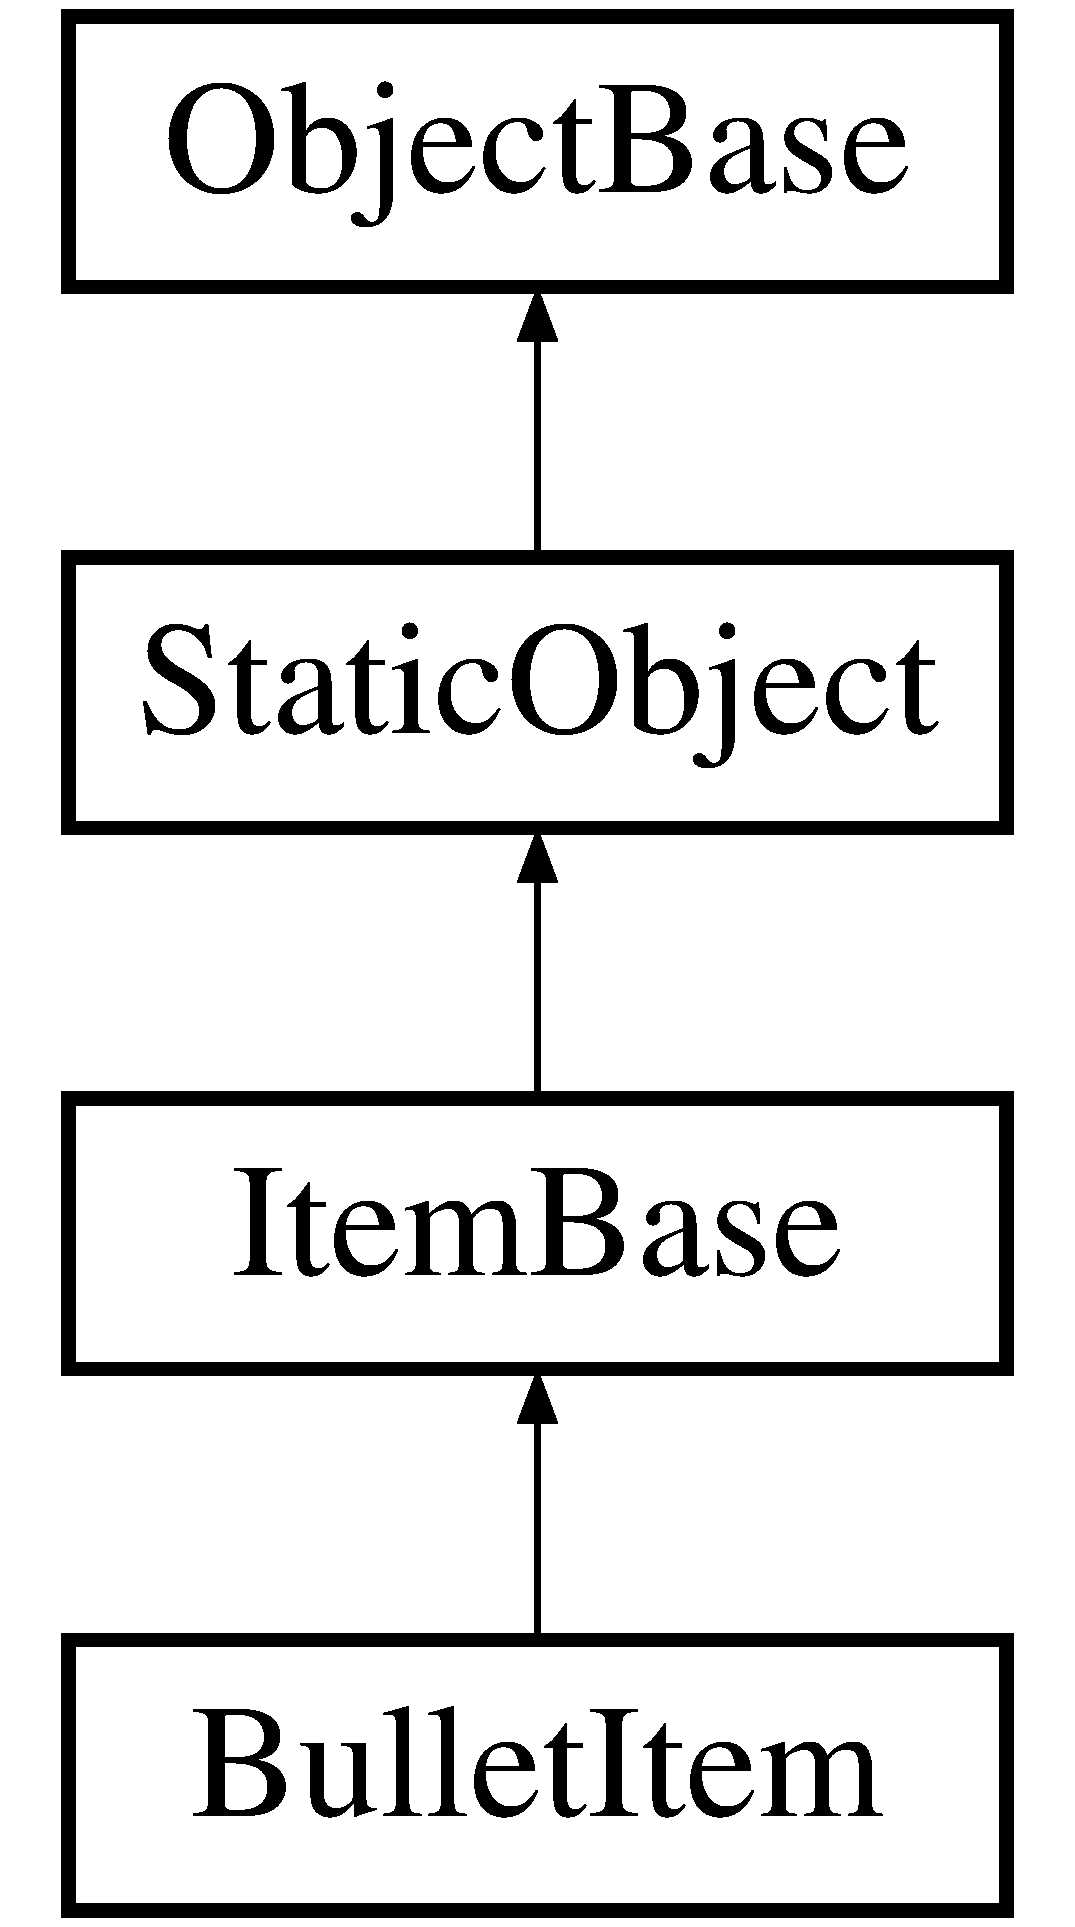
\includegraphics[height=4.000000cm]{class_bullet_item}
\end{center}
\end{figure}
\subsection*{公開メンバ関数}
\begin{DoxyCompactItemize}
\item 
\mbox{\hyperlink{class_bullet_item_a892fe09364c5392d1be1942b4ce2e466}{Bullet\+Item}} ()
\begin{DoxyCompactList}\small\item\em コンストラクタ \end{DoxyCompactList}\item 
\mbox{\hyperlink{class_bullet_item_aa72f58b22eff8a1a0efad37d9825e866}{Bullet\+Item}} (const \mbox{\hyperlink{class_bullet_item}{Bullet\+Item}} \&m)
\begin{DoxyCompactList}\small\item\em コピーコンストラクタ \end{DoxyCompactList}\item 
\mbox{\hyperlink{class_bullet_item_a6d86025339e83becf65f70b3e4c4ac49}{Bullet\+Item}} (\mbox{\hyperlink{class_bullet_item}{Bullet\+Item}} \&\&m) noexcept
\begin{DoxyCompactList}\small\item\em ムーブコンストラクタ \end{DoxyCompactList}\item 
\mbox{\hyperlink{class_bullet_item}{Bullet\+Item}} \& \mbox{\hyperlink{class_bullet_item_a0c2c6828c04646479a12dae566b41cfb}{operator=}} (const \mbox{\hyperlink{class_bullet_item}{Bullet\+Item}} \&other)
\begin{DoxyCompactList}\small\item\em コピー代入演算子 \end{DoxyCompactList}\item 
\mbox{\hyperlink{class_bullet_item}{Bullet\+Item}} \& \mbox{\hyperlink{class_bullet_item_aa494421c7189fd60911db51628c63455}{operator=}} (\mbox{\hyperlink{class_bullet_item}{Bullet\+Item}} \&\&other) noexcept
\begin{DoxyCompactList}\small\item\em ムーブ代入演算子 \end{DoxyCompactList}\end{DoxyCompactItemize}
\subsection*{その他の継承メンバ}


\subsection{構築子と解体子}
\mbox{\Hypertarget{class_bullet_item_a892fe09364c5392d1be1942b4ce2e466}\label{class_bullet_item_a892fe09364c5392d1be1942b4ce2e466}} 
\index{Bullet\+Item@{Bullet\+Item}!Bullet\+Item@{Bullet\+Item}}
\index{Bullet\+Item@{Bullet\+Item}!Bullet\+Item@{Bullet\+Item}}
\subsubsection{\texorpdfstring{Bullet\+Item()}{BulletItem()}\hspace{0.1cm}{\footnotesize\ttfamily [1/3]}}
{\footnotesize\ttfamily Bullet\+Item\+::\+Bullet\+Item (\begin{DoxyParamCaption}{ }\end{DoxyParamCaption})\hspace{0.3cm}{\ttfamily [inline]}}



コンストラクタ 

\mbox{\Hypertarget{class_bullet_item_aa72f58b22eff8a1a0efad37d9825e866}\label{class_bullet_item_aa72f58b22eff8a1a0efad37d9825e866}} 
\index{Bullet\+Item@{Bullet\+Item}!Bullet\+Item@{Bullet\+Item}}
\index{Bullet\+Item@{Bullet\+Item}!Bullet\+Item@{Bullet\+Item}}
\subsubsection{\texorpdfstring{Bullet\+Item()}{BulletItem()}\hspace{0.1cm}{\footnotesize\ttfamily [2/3]}}
{\footnotesize\ttfamily Bullet\+Item\+::\+Bullet\+Item (\begin{DoxyParamCaption}\item[{const \mbox{\hyperlink{class_bullet_item}{Bullet\+Item}} \&}]{m }\end{DoxyParamCaption})\hspace{0.3cm}{\ttfamily [inline]}}



コピーコンストラクタ 

\mbox{\Hypertarget{class_bullet_item_a6d86025339e83becf65f70b3e4c4ac49}\label{class_bullet_item_a6d86025339e83becf65f70b3e4c4ac49}} 
\index{Bullet\+Item@{Bullet\+Item}!Bullet\+Item@{Bullet\+Item}}
\index{Bullet\+Item@{Bullet\+Item}!Bullet\+Item@{Bullet\+Item}}
\subsubsection{\texorpdfstring{Bullet\+Item()}{BulletItem()}\hspace{0.1cm}{\footnotesize\ttfamily [3/3]}}
{\footnotesize\ttfamily Bullet\+Item\+::\+Bullet\+Item (\begin{DoxyParamCaption}\item[{\mbox{\hyperlink{class_bullet_item}{Bullet\+Item}} \&\&}]{m }\end{DoxyParamCaption})\hspace{0.3cm}{\ttfamily [inline]}, {\ttfamily [noexcept]}}



ムーブコンストラクタ 



\subsection{関数詳解}
\mbox{\Hypertarget{class_bullet_item_a0c2c6828c04646479a12dae566b41cfb}\label{class_bullet_item_a0c2c6828c04646479a12dae566b41cfb}} 
\index{Bullet\+Item@{Bullet\+Item}!operator=@{operator=}}
\index{operator=@{operator=}!Bullet\+Item@{Bullet\+Item}}
\subsubsection{\texorpdfstring{operator=()}{operator=()}\hspace{0.1cm}{\footnotesize\ttfamily [1/2]}}
{\footnotesize\ttfamily \mbox{\hyperlink{class_bullet_item}{Bullet\+Item}}\& Bullet\+Item\+::operator= (\begin{DoxyParamCaption}\item[{const \mbox{\hyperlink{class_bullet_item}{Bullet\+Item}} \&}]{other }\end{DoxyParamCaption})\hspace{0.3cm}{\ttfamily [inline]}}



コピー代入演算子 

\mbox{\Hypertarget{class_bullet_item_aa494421c7189fd60911db51628c63455}\label{class_bullet_item_aa494421c7189fd60911db51628c63455}} 
\index{Bullet\+Item@{Bullet\+Item}!operator=@{operator=}}
\index{operator=@{operator=}!Bullet\+Item@{Bullet\+Item}}
\subsubsection{\texorpdfstring{operator=()}{operator=()}\hspace{0.1cm}{\footnotesize\ttfamily [2/2]}}
{\footnotesize\ttfamily \mbox{\hyperlink{class_bullet_item}{Bullet\+Item}}\& Bullet\+Item\+::operator= (\begin{DoxyParamCaption}\item[{\mbox{\hyperlink{class_bullet_item}{Bullet\+Item}} \&\&}]{other }\end{DoxyParamCaption})\hspace{0.3cm}{\ttfamily [inline]}, {\ttfamily [noexcept]}}



ムーブ代入演算子 



このクラス詳解は次のファイルから抽出されました\+:\begin{DoxyCompactItemize}
\item 
C\+:/\+Users/tokir/\+Documents/\+Git\+Hub/\+Weapon\+Merchant\+Adventure/src/src/object/item/bullet/\mbox{\hyperlink{bullet__item_8h}{bullet\+\_\+item.\+h}}\end{DoxyCompactItemize}

\hypertarget{class_camera}{}\section{Camera クラス}
\label{class_camera}\index{Camera@{Camera}}


カメラクラス  




{\ttfamily \#include $<$camera.\+h$>$}

Camera の継承関係図\begin{figure}[H]
\begin{center}
\leavevmode
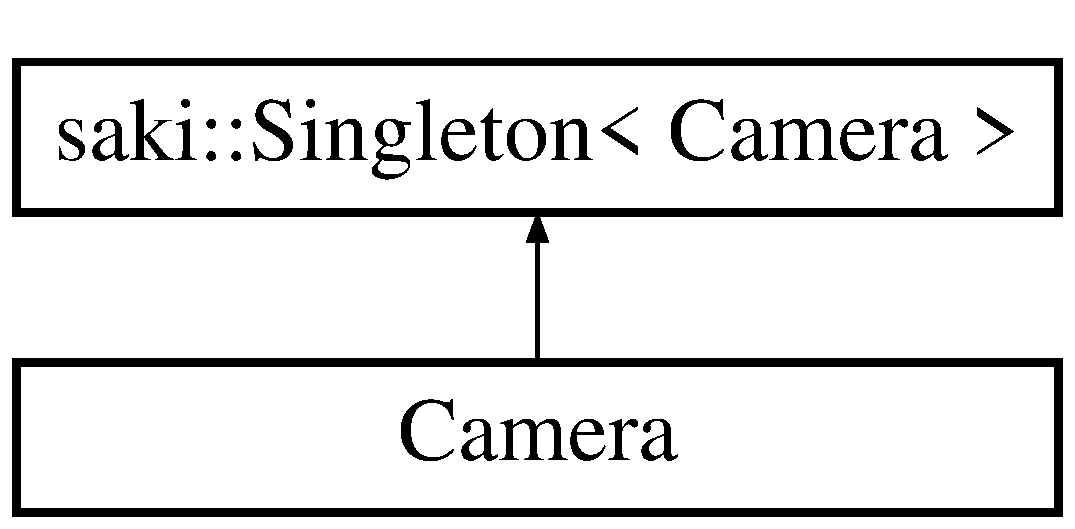
\includegraphics[height=2.000000cm]{class_camera}
\end{center}
\end{figure}
\subsection*{公開メンバ関数}
\begin{DoxyCompactItemize}
\item 
\mbox{\hyperlink{class_camera_a01f94c3543f56ede7af49dc778f19331}{Camera}} ()
\item 
\mbox{\hyperlink{class_camera_afe282ee51f1f39c041b0e7de9386cc6d}{Camera}} (const \mbox{\hyperlink{common_8h_afb0c5e21d4133ff4f200992c0b534e1b}{V\+E\+C2}} \&)
\begin{DoxyCompactList}\small\item\em カメラの値を受け取る初期化コンストラクタ \end{DoxyCompactList}\item 
void \mbox{\hyperlink{class_camera_a5c6b7ad424d835a3022393099886a90b}{Move}} (const \mbox{\hyperlink{common_8h_afb0c5e21d4133ff4f200992c0b534e1b}{V\+E\+C2}} \&)
\begin{DoxyCompactList}\small\item\em カメラの移動 \end{DoxyCompactList}\item 
void \mbox{\hyperlink{class_camera_af79aa3fedd030712e7fa122a2ea88b48}{Set\+Pos}} (const \mbox{\hyperlink{common_8h_afb0c5e21d4133ff4f200992c0b534e1b}{V\+E\+C2}} \&)
\begin{DoxyCompactList}\small\item\em カメラの位置変更 \end{DoxyCompactList}\item 
\mbox{\hyperlink{common_8h_afb0c5e21d4133ff4f200992c0b534e1b}{V\+E\+C2}} \mbox{\hyperlink{class_camera_ac3b4f1248489c0ac0faa521329de71cd}{Get\+Pos}} () const
\begin{DoxyCompactList}\small\item\em カメラの位置を取得 \end{DoxyCompactList}\item 
void \mbox{\hyperlink{class_camera_a4a596a3ea1fdc7d244ba4268031a360b}{Update}} ()
\begin{DoxyCompactList}\small\item\em カメラの更新 \end{DoxyCompactList}\item 
void \mbox{\hyperlink{class_camera_a7336f8f6c9145bee1ce6b1f16f0aaee4}{Set\+Target}} (\mbox{\hyperlink{class_object_base}{Object\+Base}} $\ast$t)
\end{DoxyCompactItemize}
\subsection*{その他の継承メンバ}


\subsection{詳解}
カメラクラス 

\subsection{構築子と解体子}
\mbox{\Hypertarget{class_camera_a01f94c3543f56ede7af49dc778f19331}\label{class_camera_a01f94c3543f56ede7af49dc778f19331}} 
\index{Camera@{Camera}!Camera@{Camera}}
\index{Camera@{Camera}!Camera@{Camera}}
\subsubsection{\texorpdfstring{Camera()}{Camera()}\hspace{0.1cm}{\footnotesize\ttfamily [1/2]}}
{\footnotesize\ttfamily Camera\+::\+Camera (\begin{DoxyParamCaption}{ }\end{DoxyParamCaption})\hspace{0.3cm}{\ttfamily [inline]}}

\mbox{\Hypertarget{class_camera_afe282ee51f1f39c041b0e7de9386cc6d}\label{class_camera_afe282ee51f1f39c041b0e7de9386cc6d}} 
\index{Camera@{Camera}!Camera@{Camera}}
\index{Camera@{Camera}!Camera@{Camera}}
\subsubsection{\texorpdfstring{Camera()}{Camera()}\hspace{0.1cm}{\footnotesize\ttfamily [2/2]}}
{\footnotesize\ttfamily Camera\+::\+Camera (\begin{DoxyParamCaption}\item[{const \mbox{\hyperlink{common_8h_afb0c5e21d4133ff4f200992c0b534e1b}{V\+E\+C2}} \&}]{v2 }\end{DoxyParamCaption})}



カメラの値を受け取る初期化コンストラクタ 


\begin{DoxyParams}{引数}
{\em v2} & 初期化する値 \\
\hline
\end{DoxyParams}


\subsection{関数詳解}
\mbox{\Hypertarget{class_camera_ac3b4f1248489c0ac0faa521329de71cd}\label{class_camera_ac3b4f1248489c0ac0faa521329de71cd}} 
\index{Camera@{Camera}!Get\+Pos@{Get\+Pos}}
\index{Get\+Pos@{Get\+Pos}!Camera@{Camera}}
\subsubsection{\texorpdfstring{Get\+Pos()}{GetPos()}}
{\footnotesize\ttfamily \mbox{\hyperlink{common_8h_afb0c5e21d4133ff4f200992c0b534e1b}{V\+E\+C2}} Camera\+::\+Get\+Pos (\begin{DoxyParamCaption}{ }\end{DoxyParamCaption}) const}



カメラの位置を取得 

\begin{DoxyReturn}{戻り値}
V\+E\+C2\+:カメラの位置 
\end{DoxyReturn}
\mbox{\Hypertarget{class_camera_a5c6b7ad424d835a3022393099886a90b}\label{class_camera_a5c6b7ad424d835a3022393099886a90b}} 
\index{Camera@{Camera}!Move@{Move}}
\index{Move@{Move}!Camera@{Camera}}
\subsubsection{\texorpdfstring{Move()}{Move()}}
{\footnotesize\ttfamily void Camera\+::\+Move (\begin{DoxyParamCaption}\item[{const \mbox{\hyperlink{common_8h_afb0c5e21d4133ff4f200992c0b534e1b}{V\+E\+C2}} \&}]{v2 }\end{DoxyParamCaption})}



カメラの移動 


\begin{DoxyParams}{引数}
{\em v2} & 移動量 \\
\hline
\end{DoxyParams}
\mbox{\Hypertarget{class_camera_af79aa3fedd030712e7fa122a2ea88b48}\label{class_camera_af79aa3fedd030712e7fa122a2ea88b48}} 
\index{Camera@{Camera}!Set\+Pos@{Set\+Pos}}
\index{Set\+Pos@{Set\+Pos}!Camera@{Camera}}
\subsubsection{\texorpdfstring{Set\+Pos()}{SetPos()}}
{\footnotesize\ttfamily void Camera\+::\+Set\+Pos (\begin{DoxyParamCaption}\item[{const \mbox{\hyperlink{common_8h_afb0c5e21d4133ff4f200992c0b534e1b}{V\+E\+C2}} \&}]{v2 }\end{DoxyParamCaption})}



カメラの位置変更 


\begin{DoxyParams}{引数}
{\em v2} & 位置 \\
\hline
\end{DoxyParams}
\mbox{\Hypertarget{class_camera_a7336f8f6c9145bee1ce6b1f16f0aaee4}\label{class_camera_a7336f8f6c9145bee1ce6b1f16f0aaee4}} 
\index{Camera@{Camera}!Set\+Target@{Set\+Target}}
\index{Set\+Target@{Set\+Target}!Camera@{Camera}}
\subsubsection{\texorpdfstring{Set\+Target()}{SetTarget()}}
{\footnotesize\ttfamily void Camera\+::\+Set\+Target (\begin{DoxyParamCaption}\item[{\mbox{\hyperlink{class_object_base}{Object\+Base}} $\ast$}]{t }\end{DoxyParamCaption})\hspace{0.3cm}{\ttfamily [inline]}}

brief ターゲットのセット \mbox{\Hypertarget{class_camera_a4a596a3ea1fdc7d244ba4268031a360b}\label{class_camera_a4a596a3ea1fdc7d244ba4268031a360b}} 
\index{Camera@{Camera}!Update@{Update}}
\index{Update@{Update}!Camera@{Camera}}
\subsubsection{\texorpdfstring{Update()}{Update()}}
{\footnotesize\ttfamily void Camera\+::\+Update (\begin{DoxyParamCaption}{ }\end{DoxyParamCaption})}



カメラの更新 



このクラス詳解は次のファイルから抽出されました\+:\begin{DoxyCompactItemize}
\item 
C\+:/\+Users/tokir/\+Documents/\+Git\+Hub/\+Weapon\+Merchant\+Adventure/src/object/camera/\mbox{\hyperlink{camera_8h}{camera.\+h}}\item 
C\+:/\+Users/tokir/\+Documents/\+Git\+Hub/\+Weapon\+Merchant\+Adventure/src/object/camera/\mbox{\hyperlink{camera_8cpp}{camera.\+cpp}}\end{DoxyCompactItemize}

\hypertarget{structsaki_1_1can__begin}{}\section{saki\+:\+:can\+\_\+begin$<$ T $>$ 構造体テンプレート}
\label{structsaki_1_1can__begin}\index{saki\+::can\+\_\+begin$<$ T $>$@{saki\+::can\+\_\+begin$<$ T $>$}}


beginできるかどうかを判定する構造体  




{\ttfamily \#include $<$can\+\_\+begin\+\_\+method.\+h$>$}

\subsection*{静的公開変数類}
\begin{DoxyCompactItemize}
\item 
static constexpr auto \mbox{\hyperlink{structsaki_1_1can__begin_a6d16b8cbacbf7d9be197d09c517d503d}{value}} = decltype(begin\+\_\+check$<$T$>$(nullptr))\+::value
\end{DoxyCompactItemize}


\subsection{詳解}
\subsubsection*{template$<$typename T$>$\newline
struct saki\+::can\+\_\+begin$<$ T $>$}

beginできるかどうかを判定する構造体 

\subsection{メンバ詳解}
\mbox{\Hypertarget{structsaki_1_1can__begin_a6d16b8cbacbf7d9be197d09c517d503d}\label{structsaki_1_1can__begin_a6d16b8cbacbf7d9be197d09c517d503d}} 
\index{saki\+::can\+\_\+begin@{saki\+::can\+\_\+begin}!value@{value}}
\index{value@{value}!saki\+::can\+\_\+begin@{saki\+::can\+\_\+begin}}
\subsubsection{\texorpdfstring{value}{value}}
{\footnotesize\ttfamily template$<$typename T $>$ \\
constexpr auto \mbox{\hyperlink{structsaki_1_1can__begin}{saki\+::can\+\_\+begin}}$<$ T $>$\+::value = decltype(begin\+\_\+check$<$T$>$(nullptr))\+::value\hspace{0.3cm}{\ttfamily [static]}}



この構造体詳解は次のファイルから抽出されました\+:\begin{DoxyCompactItemize}
\item 
C\+:/\+Users/tokir/\+Documents/\+Git\+Hub/\+Weapon\+Merchant\+Adventure/src/lib/saki/meta/\mbox{\hyperlink{can__begin__method_8h}{can\+\_\+begin\+\_\+method.\+h}}\end{DoxyCompactItemize}

\hypertarget{classsaki_1_1_clock}{}\section{saki\+:\+:Clock クラス}
\label{classsaki_1_1_clock}\index{saki\+::\+Clock@{saki\+::\+Clock}}


時間を測るクラス  




{\ttfamily \#include $<$clock.\+h$>$}

saki\+:\+:Clock の継承関係図\begin{figure}[H]
\begin{center}
\leavevmode
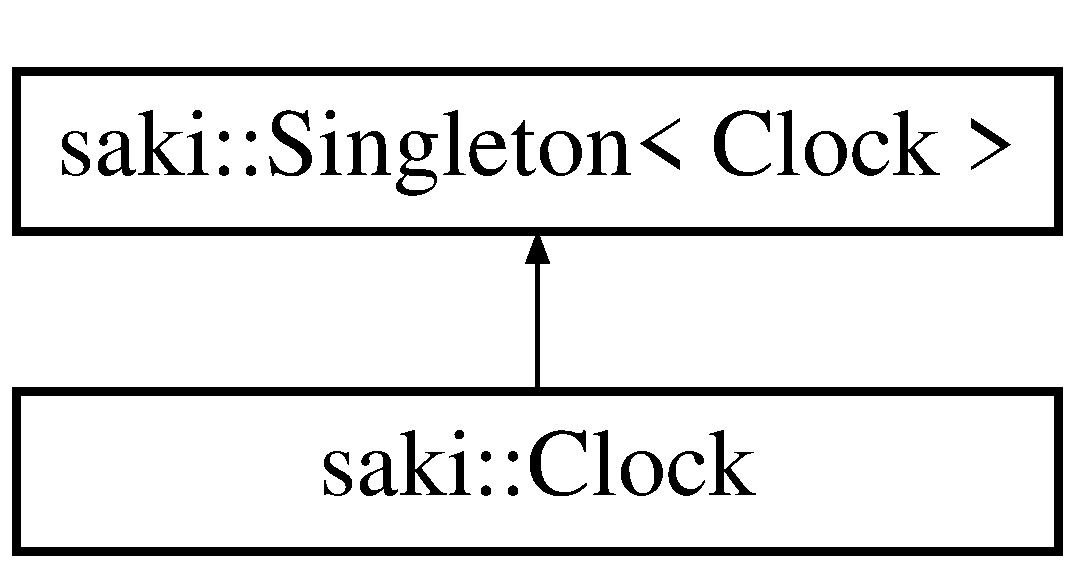
\includegraphics[height=2.000000cm]{classsaki_1_1_clock}
\end{center}
\end{figure}
\subsection*{公開メンバ関数}
\begin{DoxyCompactItemize}
\item 
\mbox{\hyperlink{classsaki_1_1_clock_a235372b9a2044bab90f38c117b49d3ab}{Clock}} ()
\begin{DoxyCompactList}\small\item\em コンストラクタ \end{DoxyCompactList}\item 
void \mbox{\hyperlink{classsaki_1_1_clock_a522e7d5dcae1f457dfc1cd4eb9560cec}{start}} ()
\begin{DoxyCompactList}\small\item\em 開始時間のセット \end{DoxyCompactList}\item 
{\footnotesize template$<$typename T  = double$>$ }\\T \mbox{\hyperlink{classsaki_1_1_clock_afb3a41ac314bb58c010283bea60069f9}{end}} (bool ms=true)
\begin{DoxyCompactList}\small\item\em 開始時間をセットしてからの時間を返す \end{DoxyCompactList}\item 
{\footnotesize template$<$typename T  = double$>$ }\\T \mbox{\hyperlink{classsaki_1_1_clock_a6df6705089065ac8f9f3cdb718d7284f}{end\+\_\+and\+\_\+start}} (bool ms=true)
\begin{DoxyCompactList}\small\item\em 開始時間をセットしてからの時間を返し、そこからまた時間をスタートする \end{DoxyCompactList}\end{DoxyCompactItemize}
\subsection*{その他の継承メンバ}


\subsection{詳解}
時間を測るクラス 

\subsection{構築子と解体子}
\mbox{\Hypertarget{classsaki_1_1_clock_a235372b9a2044bab90f38c117b49d3ab}\label{classsaki_1_1_clock_a235372b9a2044bab90f38c117b49d3ab}} 
\index{saki\+::\+Clock@{saki\+::\+Clock}!Clock@{Clock}}
\index{Clock@{Clock}!saki\+::\+Clock@{saki\+::\+Clock}}
\subsubsection{\texorpdfstring{Clock()}{Clock()}}
{\footnotesize\ttfamily saki\+::\+Clock\+::\+Clock (\begin{DoxyParamCaption}{ }\end{DoxyParamCaption})\hspace{0.3cm}{\ttfamily [inline]}}



コンストラクタ 



\subsection{関数詳解}
\mbox{\Hypertarget{classsaki_1_1_clock_afb3a41ac314bb58c010283bea60069f9}\label{classsaki_1_1_clock_afb3a41ac314bb58c010283bea60069f9}} 
\index{saki\+::\+Clock@{saki\+::\+Clock}!end@{end}}
\index{end@{end}!saki\+::\+Clock@{saki\+::\+Clock}}
\subsubsection{\texorpdfstring{end()}{end()}}
{\footnotesize\ttfamily template$<$typename T  = double$>$ \\
T saki\+::\+Clock\+::end (\begin{DoxyParamCaption}\item[{bool}]{ms = {\ttfamily true} }\end{DoxyParamCaption})\hspace{0.3cm}{\ttfamily [inline]}}



開始時間をセットしてからの時間を返す 


\begin{DoxyParams}{引数}
{\em ms} & trueならミリ秒,falseなら秒で返す return 時間 \\
\hline
\end{DoxyParams}
\mbox{\Hypertarget{classsaki_1_1_clock_a6df6705089065ac8f9f3cdb718d7284f}\label{classsaki_1_1_clock_a6df6705089065ac8f9f3cdb718d7284f}} 
\index{saki\+::\+Clock@{saki\+::\+Clock}!end\+\_\+and\+\_\+start@{end\+\_\+and\+\_\+start}}
\index{end\+\_\+and\+\_\+start@{end\+\_\+and\+\_\+start}!saki\+::\+Clock@{saki\+::\+Clock}}
\subsubsection{\texorpdfstring{end\+\_\+and\+\_\+start()}{end\_and\_start()}}
{\footnotesize\ttfamily template$<$typename T  = double$>$ \\
T saki\+::\+Clock\+::end\+\_\+and\+\_\+start (\begin{DoxyParamCaption}\item[{bool}]{ms = {\ttfamily true} }\end{DoxyParamCaption})\hspace{0.3cm}{\ttfamily [inline]}}



開始時間をセットしてからの時間を返し、そこからまた時間をスタートする 


\begin{DoxyParams}{引数}
{\em ms} & trueならミリ秒,falseなら秒で返す return 時間 \\
\hline
\end{DoxyParams}
\mbox{\Hypertarget{classsaki_1_1_clock_a522e7d5dcae1f457dfc1cd4eb9560cec}\label{classsaki_1_1_clock_a522e7d5dcae1f457dfc1cd4eb9560cec}} 
\index{saki\+::\+Clock@{saki\+::\+Clock}!start@{start}}
\index{start@{start}!saki\+::\+Clock@{saki\+::\+Clock}}
\subsubsection{\texorpdfstring{start()}{start()}}
{\footnotesize\ttfamily void saki\+::\+Clock\+::start (\begin{DoxyParamCaption}{ }\end{DoxyParamCaption})\hspace{0.3cm}{\ttfamily [inline]}}



開始時間のセット 



このクラス詳解は次のファイルから抽出されました\+:\begin{DoxyCompactItemize}
\item 
C\+:/\+Users/tokir/\+Documents/\+Git\+Hub/\+Weapon\+Merchant\+Adventure/src/lib/saki/clock/\mbox{\hyperlink{clock_8h}{clock.\+h}}\end{DoxyCompactItemize}

\hypertarget{class_collider_base}{}\section{Collider\+Base クラス}
\label{class_collider_base}\index{Collider\+Base@{Collider\+Base}}


コライダのスーパークラス  




{\ttfamily \#include $<$collider\+\_\+base.\+h$>$}

Collider\+Base の継承関係図\begin{figure}[H]
\begin{center}
\leavevmode
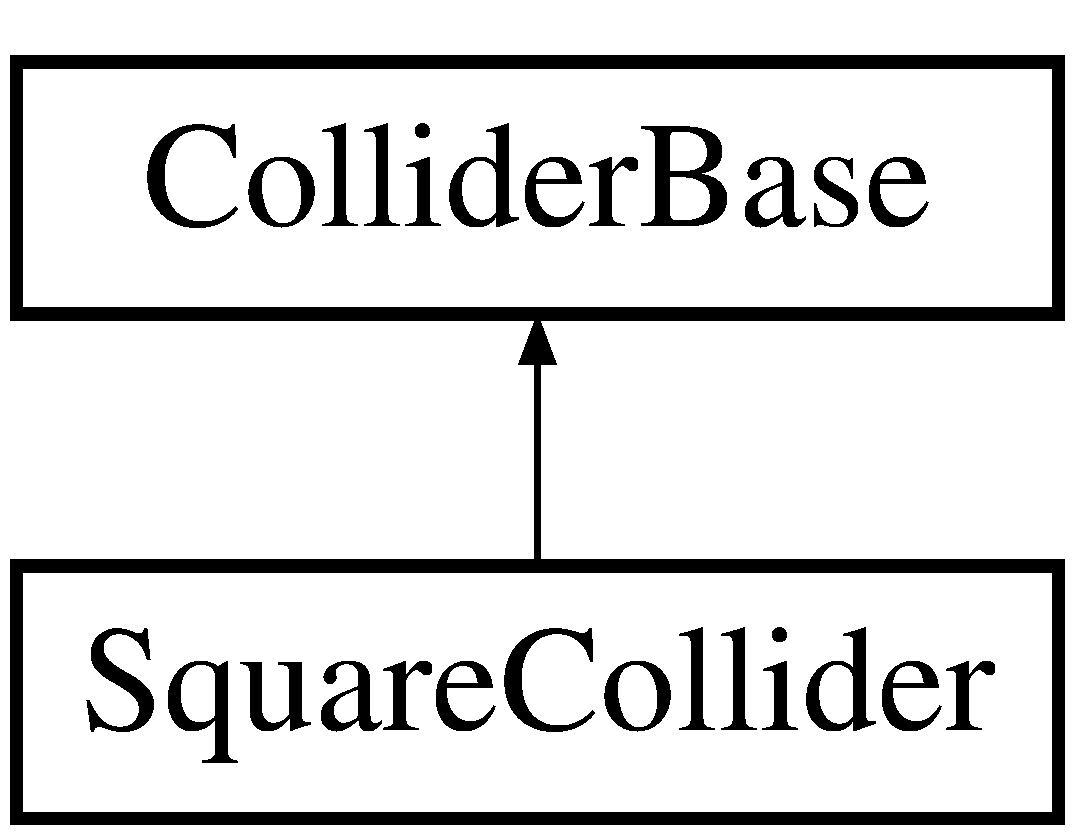
\includegraphics[height=2.000000cm]{class_collider_base}
\end{center}
\end{figure}
\subsection*{公開メンバ関数}
\begin{DoxyCompactItemize}
\item 
\mbox{\hyperlink{class_collider_base_a61d7057a7e05549088f2b15c1e525858}{Collider\+Base}} (\mbox{\hyperlink{class_object_base}{Object\+Base}} $\ast$obj, bool \+\_\+is\+\_\+trigger=false)
\begin{DoxyCompactList}\small\item\em コンストラクタ \end{DoxyCompactList}\item 
\mbox{\hyperlink{class_collider_base}{Collider\+Base}} \& \mbox{\hyperlink{class_collider_base_a2bc4d08eb29126c0cb0ea45b06517328}{operator=}} (const \mbox{\hyperlink{class_collider_base}{Collider\+Base}} \&other)
\begin{DoxyCompactList}\small\item\em コピー代入演算子 \end{DoxyCompactList}\item 
virtual \mbox{\hyperlink{class_collider_base_a485c8a6348a053228aa61142a71e48fb}{$\sim$\+Collider\+Base}} ()
\end{DoxyCompactItemize}
\subsection*{公開変数類}
\begin{DoxyCompactItemize}
\item 
bool \mbox{\hyperlink{class_collider_base_a1943a8429f6ef2cce5785975cba321b1}{collision\+\_\+destroy}} = false
\item 
bool \mbox{\hyperlink{class_collider_base_a8e2383d9422880103aa5309a6dfcef48}{is\+\_\+trigger}}
\item 
bool \mbox{\hyperlink{class_collider_base_a7e6348c051a8c01ff7884d366bd292eb}{collision\+\_\+is\+\_\+static\+\_\+x}} = false
\item 
bool \mbox{\hyperlink{class_collider_base_a5a50a0f911a108eba730de1b22c1cc9e}{collision\+\_\+is\+\_\+static\+\_\+y}} = false
\item 
\mbox{\hyperlink{class_object_base}{Object\+Base}} $\ast$ \mbox{\hyperlink{class_collider_base_a63adac6a75877857abe9ff2cf4274157}{object}}
\item 
std\+::function$<$ void(\mbox{\hyperlink{class_object_base}{Object\+Base}} $\ast$, \mbox{\hyperlink{common_8h_afb0c5e21d4133ff4f200992c0b534e1b}{V\+E\+C2}})$>$ \mbox{\hyperlink{class_collider_base_a5ac4f3c76c753790abef75e3eb7accbe}{collision\+\_\+func}}
\item 
bool \mbox{\hyperlink{class_collider_base_a812053f247dc6357357bdf9353dded77}{enabled}} = true
\end{DoxyCompactItemize}


\subsection{詳解}
コライダのスーパークラス 

\subsection{構築子と解体子}
\mbox{\Hypertarget{class_collider_base_a61d7057a7e05549088f2b15c1e525858}\label{class_collider_base_a61d7057a7e05549088f2b15c1e525858}} 
\index{Collider\+Base@{Collider\+Base}!Collider\+Base@{Collider\+Base}}
\index{Collider\+Base@{Collider\+Base}!Collider\+Base@{Collider\+Base}}
\subsubsection{\texorpdfstring{Collider\+Base()}{ColliderBase()}}
{\footnotesize\ttfamily Collider\+Base\+::\+Collider\+Base (\begin{DoxyParamCaption}\item[{\mbox{\hyperlink{class_object_base}{Object\+Base}} $\ast$}]{obj,  }\item[{bool}]{\+\_\+is\+\_\+trigger = {\ttfamily false} }\end{DoxyParamCaption})\hspace{0.3cm}{\ttfamily [inline]}}



コンストラクタ 


\begin{DoxyParams}{引数}
{\em obj} & オブジェクト \\
\hline
{\em \+\_\+is\+\_\+trigger} & 押し出しするかどうか \\
\hline
\end{DoxyParams}
\mbox{\Hypertarget{class_collider_base_a485c8a6348a053228aa61142a71e48fb}\label{class_collider_base_a485c8a6348a053228aa61142a71e48fb}} 
\index{Collider\+Base@{Collider\+Base}!````~Collider\+Base@{$\sim$\+Collider\+Base}}
\index{````~Collider\+Base@{$\sim$\+Collider\+Base}!Collider\+Base@{Collider\+Base}}
\subsubsection{\texorpdfstring{$\sim$\+Collider\+Base()}{~ColliderBase()}}
{\footnotesize\ttfamily virtual Collider\+Base\+::$\sim$\+Collider\+Base (\begin{DoxyParamCaption}{ }\end{DoxyParamCaption})\hspace{0.3cm}{\ttfamily [inline]}, {\ttfamily [virtual]}}



\subsection{関数詳解}
\mbox{\Hypertarget{class_collider_base_a2bc4d08eb29126c0cb0ea45b06517328}\label{class_collider_base_a2bc4d08eb29126c0cb0ea45b06517328}} 
\index{Collider\+Base@{Collider\+Base}!operator=@{operator=}}
\index{operator=@{operator=}!Collider\+Base@{Collider\+Base}}
\subsubsection{\texorpdfstring{operator=()}{operator=()}}
{\footnotesize\ttfamily \mbox{\hyperlink{class_collider_base}{Collider\+Base}}\& Collider\+Base\+::operator= (\begin{DoxyParamCaption}\item[{const \mbox{\hyperlink{class_collider_base}{Collider\+Base}} \&}]{other }\end{DoxyParamCaption})\hspace{0.3cm}{\ttfamily [inline]}}



コピー代入演算子 



\subsection{メンバ詳解}
\mbox{\Hypertarget{class_collider_base_a1943a8429f6ef2cce5785975cba321b1}\label{class_collider_base_a1943a8429f6ef2cce5785975cba321b1}} 
\index{Collider\+Base@{Collider\+Base}!collision\+\_\+destroy@{collision\+\_\+destroy}}
\index{collision\+\_\+destroy@{collision\+\_\+destroy}!Collider\+Base@{Collider\+Base}}
\subsubsection{\texorpdfstring{collision\+\_\+destroy}{collision\_destroy}}
{\footnotesize\ttfamily bool Collider\+Base\+::collision\+\_\+destroy = false}

\mbox{\Hypertarget{class_collider_base_a5ac4f3c76c753790abef75e3eb7accbe}\label{class_collider_base_a5ac4f3c76c753790abef75e3eb7accbe}} 
\index{Collider\+Base@{Collider\+Base}!collision\+\_\+func@{collision\+\_\+func}}
\index{collision\+\_\+func@{collision\+\_\+func}!Collider\+Base@{Collider\+Base}}
\subsubsection{\texorpdfstring{collision\+\_\+func}{collision\_func}}
{\footnotesize\ttfamily std\+::function$<$void(\mbox{\hyperlink{class_object_base}{Object\+Base}}$\ast$,\mbox{\hyperlink{common_8h_afb0c5e21d4133ff4f200992c0b534e1b}{V\+E\+C2}})$>$ Collider\+Base\+::collision\+\_\+func}

\mbox{\Hypertarget{class_collider_base_a7e6348c051a8c01ff7884d366bd292eb}\label{class_collider_base_a7e6348c051a8c01ff7884d366bd292eb}} 
\index{Collider\+Base@{Collider\+Base}!collision\+\_\+is\+\_\+static\+\_\+x@{collision\+\_\+is\+\_\+static\+\_\+x}}
\index{collision\+\_\+is\+\_\+static\+\_\+x@{collision\+\_\+is\+\_\+static\+\_\+x}!Collider\+Base@{Collider\+Base}}
\subsubsection{\texorpdfstring{collision\+\_\+is\+\_\+static\+\_\+x}{collision\_is\_static\_x}}
{\footnotesize\ttfamily bool Collider\+Base\+::collision\+\_\+is\+\_\+static\+\_\+x = false}

\mbox{\Hypertarget{class_collider_base_a5a50a0f911a108eba730de1b22c1cc9e}\label{class_collider_base_a5a50a0f911a108eba730de1b22c1cc9e}} 
\index{Collider\+Base@{Collider\+Base}!collision\+\_\+is\+\_\+static\+\_\+y@{collision\+\_\+is\+\_\+static\+\_\+y}}
\index{collision\+\_\+is\+\_\+static\+\_\+y@{collision\+\_\+is\+\_\+static\+\_\+y}!Collider\+Base@{Collider\+Base}}
\subsubsection{\texorpdfstring{collision\+\_\+is\+\_\+static\+\_\+y}{collision\_is\_static\_y}}
{\footnotesize\ttfamily bool Collider\+Base\+::collision\+\_\+is\+\_\+static\+\_\+y = false}

\mbox{\Hypertarget{class_collider_base_a812053f247dc6357357bdf9353dded77}\label{class_collider_base_a812053f247dc6357357bdf9353dded77}} 
\index{Collider\+Base@{Collider\+Base}!enabled@{enabled}}
\index{enabled@{enabled}!Collider\+Base@{Collider\+Base}}
\subsubsection{\texorpdfstring{enabled}{enabled}}
{\footnotesize\ttfamily bool Collider\+Base\+::enabled = true}

\mbox{\Hypertarget{class_collider_base_a8e2383d9422880103aa5309a6dfcef48}\label{class_collider_base_a8e2383d9422880103aa5309a6dfcef48}} 
\index{Collider\+Base@{Collider\+Base}!is\+\_\+trigger@{is\+\_\+trigger}}
\index{is\+\_\+trigger@{is\+\_\+trigger}!Collider\+Base@{Collider\+Base}}
\subsubsection{\texorpdfstring{is\+\_\+trigger}{is\_trigger}}
{\footnotesize\ttfamily bool Collider\+Base\+::is\+\_\+trigger}

\mbox{\Hypertarget{class_collider_base_a63adac6a75877857abe9ff2cf4274157}\label{class_collider_base_a63adac6a75877857abe9ff2cf4274157}} 
\index{Collider\+Base@{Collider\+Base}!object@{object}}
\index{object@{object}!Collider\+Base@{Collider\+Base}}
\subsubsection{\texorpdfstring{object}{object}}
{\footnotesize\ttfamily \mbox{\hyperlink{class_object_base}{Object\+Base}}$\ast$ Collider\+Base\+::object}



このクラス詳解は次のファイルから抽出されました\+:\begin{DoxyCompactItemize}
\item 
C\+:/\+Users/tokir/\+Documents/\+Git\+Hub/\+Weapon\+Merchant\+Adventure/src/collider/base/\mbox{\hyperlink{collider__base_8h}{collider\+\_\+base.\+h}}\end{DoxyCompactItemize}

\hypertarget{class_collider_manager}{}\section{Collider\+Manager クラス}
\label{class_collider_manager}\index{Collider\+Manager@{Collider\+Manager}}


コライダを管理するクラス  




{\ttfamily \#include $<$collider\+\_\+manager.\+h$>$}

Collider\+Manager の継承関係図\begin{figure}[H]
\begin{center}
\leavevmode
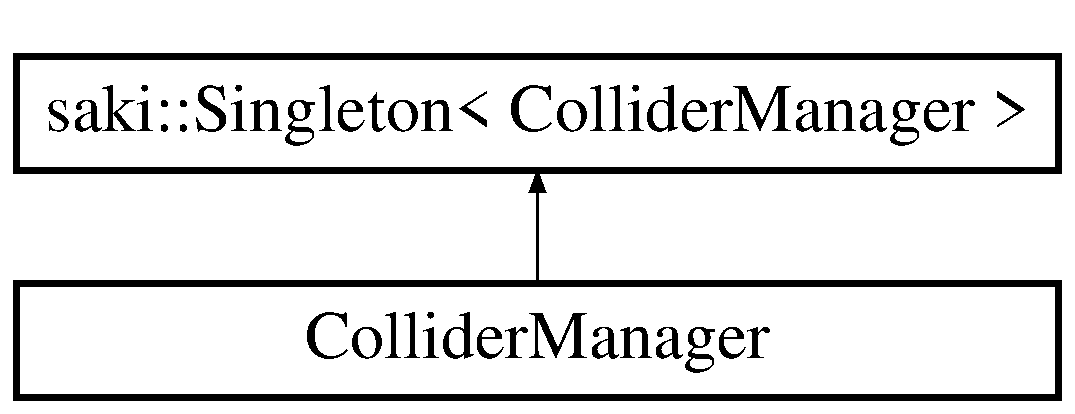
\includegraphics[height=2.000000cm]{class_collider_manager}
\end{center}
\end{figure}
\subsection*{公開メンバ関数}
\begin{DoxyCompactItemize}
\item 
void \mbox{\hyperlink{class_collider_manager_a9e6c7ca21ae4e79fdf4892982e72bc99}{Set\+Square\+Collider}} (\mbox{\hyperlink{class_square_collider}{Square\+Collider}} $\ast$, bool is\+\_\+static)
\begin{DoxyCompactList}\small\item\em コライダを配列に格納する \end{DoxyCompactList}\item 
void \mbox{\hyperlink{class_collider_manager_af3863143e206b4c86c8b89dd91ff3c8c}{Check\+Collision}} ()
\begin{DoxyCompactList}\small\item\em 全てのコライダを走査する \end{DoxyCompactList}\item 
void \mbox{\hyperlink{class_collider_manager_a24df637a6f092602b547c6a2bd773113}{Delete\+Square\+Collider}} (\mbox{\hyperlink{class_square_collider}{Square\+Collider}} $\ast$)
\begin{DoxyCompactList}\small\item\em 四角形コライダの削除 \end{DoxyCompactList}\end{DoxyCompactItemize}
\subsection*{限定公開メンバ関数}
\begin{DoxyCompactItemize}
\item 
bool \mbox{\hyperlink{class_collider_manager_a612f6096ca24702bff6dee04a88a40c3}{Compare\+Square\+Square\+Collision}} (const \mbox{\hyperlink{class_square_collider}{Square\+Collider}} $\ast$, const \mbox{\hyperlink{class_square_collider}{Square\+Collider}} $\ast$)
\begin{DoxyCompactList}\small\item\em 四角形同士が当たっているかを判定する \end{DoxyCompactList}\end{DoxyCompactItemize}
\subsection*{その他の継承メンバ}


\subsection{詳解}
コライダを管理するクラス 

\subsection{関数詳解}
\mbox{\Hypertarget{class_collider_manager_af3863143e206b4c86c8b89dd91ff3c8c}\label{class_collider_manager_af3863143e206b4c86c8b89dd91ff3c8c}} 
\index{Collider\+Manager@{Collider\+Manager}!Check\+Collision@{Check\+Collision}}
\index{Check\+Collision@{Check\+Collision}!Collider\+Manager@{Collider\+Manager}}
\subsubsection{\texorpdfstring{Check\+Collision()}{CheckCollision()}}
{\footnotesize\ttfamily void Collider\+Manager\+::\+Check\+Collision (\begin{DoxyParamCaption}{ }\end{DoxyParamCaption})}



全てのコライダを走査する 

\mbox{\Hypertarget{class_collider_manager_a612f6096ca24702bff6dee04a88a40c3}\label{class_collider_manager_a612f6096ca24702bff6dee04a88a40c3}} 
\index{Collider\+Manager@{Collider\+Manager}!Compare\+Square\+Square\+Collision@{Compare\+Square\+Square\+Collision}}
\index{Compare\+Square\+Square\+Collision@{Compare\+Square\+Square\+Collision}!Collider\+Manager@{Collider\+Manager}}
\subsubsection{\texorpdfstring{Compare\+Square\+Square\+Collision()}{CompareSquareSquareCollision()}}
{\footnotesize\ttfamily bool Collider\+Manager\+::\+Compare\+Square\+Square\+Collision (\begin{DoxyParamCaption}\item[{const \mbox{\hyperlink{class_square_collider}{Square\+Collider}} $\ast$}]{col1,  }\item[{const \mbox{\hyperlink{class_square_collider}{Square\+Collider}} $\ast$}]{col2 }\end{DoxyParamCaption})\hspace{0.3cm}{\ttfamily [protected]}}



四角形同士が当たっているかを判定する 


\begin{DoxyParams}{引数}
{\em col1,col2} & 比べる二つの四角形コライダ \\
\hline
\end{DoxyParams}
\begin{DoxyReturn}{戻り値}
bool 当たっているかどうか 
\end{DoxyReturn}
\mbox{\Hypertarget{class_collider_manager_a24df637a6f092602b547c6a2bd773113}\label{class_collider_manager_a24df637a6f092602b547c6a2bd773113}} 
\index{Collider\+Manager@{Collider\+Manager}!Delete\+Square\+Collider@{Delete\+Square\+Collider}}
\index{Delete\+Square\+Collider@{Delete\+Square\+Collider}!Collider\+Manager@{Collider\+Manager}}
\subsubsection{\texorpdfstring{Delete\+Square\+Collider()}{DeleteSquareCollider()}}
{\footnotesize\ttfamily void Collider\+Manager\+::\+Delete\+Square\+Collider (\begin{DoxyParamCaption}\item[{\mbox{\hyperlink{class_square_collider}{Square\+Collider}} $\ast$}]{col }\end{DoxyParamCaption})}



四角形コライダの削除 


\begin{DoxyParams}{引数}
{\em col} & 四角形コライダ \\
\hline
\end{DoxyParams}
\mbox{\Hypertarget{class_collider_manager_a9e6c7ca21ae4e79fdf4892982e72bc99}\label{class_collider_manager_a9e6c7ca21ae4e79fdf4892982e72bc99}} 
\index{Collider\+Manager@{Collider\+Manager}!Set\+Square\+Collider@{Set\+Square\+Collider}}
\index{Set\+Square\+Collider@{Set\+Square\+Collider}!Collider\+Manager@{Collider\+Manager}}
\subsubsection{\texorpdfstring{Set\+Square\+Collider()}{SetSquareCollider()}}
{\footnotesize\ttfamily void Collider\+Manager\+::\+Set\+Square\+Collider (\begin{DoxyParamCaption}\item[{\mbox{\hyperlink{class_square_collider}{Square\+Collider}} $\ast$}]{obj,  }\item[{bool}]{is\+\_\+static }\end{DoxyParamCaption})}



コライダを配列に格納する 


\begin{DoxyParams}{引数}
{\em obj} & 当たり判定クラス \\
\hline
{\em is\+\_\+static} & 静的か動的か \\
\hline
\end{DoxyParams}


このクラス詳解は次のファイルから抽出されました\+:\begin{DoxyCompactItemize}
\item 
C\+:/\+Users/tokir/\+Documents/\+Git\+Hub/\+Weapon\+Merchant\+Adventure/src/collider/manager/\mbox{\hyperlink{collider__manager_8h}{collider\+\_\+manager.\+h}}\item 
C\+:/\+Users/tokir/\+Documents/\+Git\+Hub/\+Weapon\+Merchant\+Adventure/src/collider/manager/\mbox{\hyperlink{collider__manager_8cpp}{collider\+\_\+manager.\+cpp}}\end{DoxyCompactItemize}

\hypertarget{class_device}{}\section{Device クラス}
\label{class_device}\index{Device@{Device}}


{\ttfamily \#include $<$device.\+h$>$}

Device の継承関係図\begin{figure}[H]
\begin{center}
\leavevmode
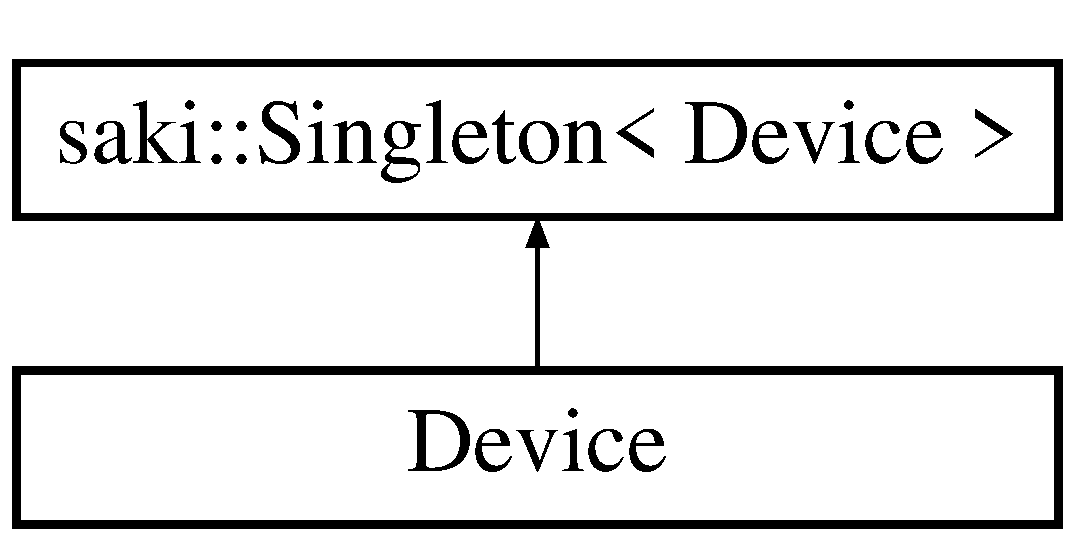
\includegraphics[height=2.000000cm]{class_device}
\end{center}
\end{figure}
\subsection*{公開メンバ関数}
\begin{DoxyCompactItemize}
\item 
H\+R\+E\+S\+U\+LT \mbox{\hyperlink{class_device_a8fc449792bf98bab448683f6815446e9}{init}} (H\+W\+ND)
\item 
void \mbox{\hyperlink{class_device_a17cd76103195bae419de11d43a4eeecd}{clear\+\_\+screen}} ()
\item 
void \mbox{\hyperlink{class_device_a066c09b28fab69581e18459f45daa6a6}{draw\+\_\+begin}} ()
\item 
void \mbox{\hyperlink{class_device_aa7c7313576c3274087b872a915fa181e}{draw\+\_\+end}} ()
\end{DoxyCompactItemize}
\subsection*{公開変数類}
\begin{DoxyCompactItemize}
\item 
\mbox{\hyperlink{common_8h_ab7d7d9064a34dd725663b1dbee652aca}{Com\+Ptr}}$<$ I\+D3\+D11\+Device $>$ \mbox{\hyperlink{class_device_af0aeb4e2375287fe02fc5154015b53be}{device}}
\item 
\mbox{\hyperlink{common_8h_ab7d7d9064a34dd725663b1dbee652aca}{Com\+Ptr}}$<$ I\+D3\+D11\+Device\+Context $>$ \mbox{\hyperlink{class_device_a445dfbc67c6d8ad039ee462a891d63fc}{immediate\+\_\+context}}
\item 
\mbox{\hyperlink{common_8h_ab7d7d9064a34dd725663b1dbee652aca}{Com\+Ptr}}$<$ I\+D\+X\+G\+I\+Swap\+Chain $>$ \mbox{\hyperlink{class_device_a8e522e4b61ad77b6581d4a160234c790}{swap\+\_\+chain}}
\item 
\mbox{\hyperlink{common_8h_ab7d7d9064a34dd725663b1dbee652aca}{Com\+Ptr}}$<$ I\+D3\+D11\+Render\+Target\+View $>$ \mbox{\hyperlink{class_device_ad50562d65b7c377ff48bf3ca26555028}{render\+\_\+target\+\_\+view}}
\item 
\mbox{\hyperlink{common_8h_ab7d7d9064a34dd725663b1dbee652aca}{Com\+Ptr}}$<$ I\+D3\+D11\+Depth\+Stencil\+View $>$ \mbox{\hyperlink{class_device_ac76a2dc2c3c49bb40f82c6d5300bf2b8}{depth\+\_\+stencil\+\_\+view}}
\item 
\mbox{\hyperlink{common_8h_ab7d7d9064a34dd725663b1dbee652aca}{Com\+Ptr}}$<$ I\+D3\+D11\+Texture2D $>$ \mbox{\hyperlink{class_device_a077098001481f1c1c0c274caba595625}{depth\+\_\+stencil\+\_\+texture}}
\end{DoxyCompactItemize}
\subsection*{その他の継承メンバ}


\subsection{関数詳解}
\mbox{\Hypertarget{class_device_a17cd76103195bae419de11d43a4eeecd}\label{class_device_a17cd76103195bae419de11d43a4eeecd}} 
\index{Device@{Device}!clear\+\_\+screen@{clear\+\_\+screen}}
\index{clear\+\_\+screen@{clear\+\_\+screen}!Device@{Device}}
\subsubsection{\texorpdfstring{clear\+\_\+screen()}{clear\_screen()}}
{\footnotesize\ttfamily void Device\+::clear\+\_\+screen (\begin{DoxyParamCaption}{ }\end{DoxyParamCaption})}

\mbox{\Hypertarget{class_device_a066c09b28fab69581e18459f45daa6a6}\label{class_device_a066c09b28fab69581e18459f45daa6a6}} 
\index{Device@{Device}!draw\+\_\+begin@{draw\+\_\+begin}}
\index{draw\+\_\+begin@{draw\+\_\+begin}!Device@{Device}}
\subsubsection{\texorpdfstring{draw\+\_\+begin()}{draw\_begin()}}
{\footnotesize\ttfamily void Device\+::draw\+\_\+begin (\begin{DoxyParamCaption}{ }\end{DoxyParamCaption})\hspace{0.3cm}{\ttfamily [inline]}}

\mbox{\Hypertarget{class_device_aa7c7313576c3274087b872a915fa181e}\label{class_device_aa7c7313576c3274087b872a915fa181e}} 
\index{Device@{Device}!draw\+\_\+end@{draw\+\_\+end}}
\index{draw\+\_\+end@{draw\+\_\+end}!Device@{Device}}
\subsubsection{\texorpdfstring{draw\+\_\+end()}{draw\_end()}}
{\footnotesize\ttfamily void Device\+::draw\+\_\+end (\begin{DoxyParamCaption}{ }\end{DoxyParamCaption})\hspace{0.3cm}{\ttfamily [inline]}}

\mbox{\Hypertarget{class_device_a8fc449792bf98bab448683f6815446e9}\label{class_device_a8fc449792bf98bab448683f6815446e9}} 
\index{Device@{Device}!init@{init}}
\index{init@{init}!Device@{Device}}
\subsubsection{\texorpdfstring{init()}{init()}}
{\footnotesize\ttfamily H\+R\+E\+S\+U\+LT Device\+::init (\begin{DoxyParamCaption}\item[{H\+W\+ND}]{hwnd }\end{DoxyParamCaption})}



\subsection{メンバ詳解}
\mbox{\Hypertarget{class_device_a077098001481f1c1c0c274caba595625}\label{class_device_a077098001481f1c1c0c274caba595625}} 
\index{Device@{Device}!depth\+\_\+stencil\+\_\+texture@{depth\+\_\+stencil\+\_\+texture}}
\index{depth\+\_\+stencil\+\_\+texture@{depth\+\_\+stencil\+\_\+texture}!Device@{Device}}
\subsubsection{\texorpdfstring{depth\+\_\+stencil\+\_\+texture}{depth\_stencil\_texture}}
{\footnotesize\ttfamily \mbox{\hyperlink{common_8h_ab7d7d9064a34dd725663b1dbee652aca}{Com\+Ptr}}$<$I\+D3\+D11\+Texture2D$>$ Device\+::depth\+\_\+stencil\+\_\+texture}

\mbox{\Hypertarget{class_device_ac76a2dc2c3c49bb40f82c6d5300bf2b8}\label{class_device_ac76a2dc2c3c49bb40f82c6d5300bf2b8}} 
\index{Device@{Device}!depth\+\_\+stencil\+\_\+view@{depth\+\_\+stencil\+\_\+view}}
\index{depth\+\_\+stencil\+\_\+view@{depth\+\_\+stencil\+\_\+view}!Device@{Device}}
\subsubsection{\texorpdfstring{depth\+\_\+stencil\+\_\+view}{depth\_stencil\_view}}
{\footnotesize\ttfamily \mbox{\hyperlink{common_8h_ab7d7d9064a34dd725663b1dbee652aca}{Com\+Ptr}}$<$I\+D3\+D11\+Depth\+Stencil\+View$>$ Device\+::depth\+\_\+stencil\+\_\+view}

\mbox{\Hypertarget{class_device_af0aeb4e2375287fe02fc5154015b53be}\label{class_device_af0aeb4e2375287fe02fc5154015b53be}} 
\index{Device@{Device}!device@{device}}
\index{device@{device}!Device@{Device}}
\subsubsection{\texorpdfstring{device}{device}}
{\footnotesize\ttfamily \mbox{\hyperlink{common_8h_ab7d7d9064a34dd725663b1dbee652aca}{Com\+Ptr}}$<$I\+D3\+D11\+Device$>$ Device\+::device}

\mbox{\Hypertarget{class_device_a445dfbc67c6d8ad039ee462a891d63fc}\label{class_device_a445dfbc67c6d8ad039ee462a891d63fc}} 
\index{Device@{Device}!immediate\+\_\+context@{immediate\+\_\+context}}
\index{immediate\+\_\+context@{immediate\+\_\+context}!Device@{Device}}
\subsubsection{\texorpdfstring{immediate\+\_\+context}{immediate\_context}}
{\footnotesize\ttfamily \mbox{\hyperlink{common_8h_ab7d7d9064a34dd725663b1dbee652aca}{Com\+Ptr}}$<$I\+D3\+D11\+Device\+Context$>$ Device\+::immediate\+\_\+context}

\mbox{\Hypertarget{class_device_ad50562d65b7c377ff48bf3ca26555028}\label{class_device_ad50562d65b7c377ff48bf3ca26555028}} 
\index{Device@{Device}!render\+\_\+target\+\_\+view@{render\+\_\+target\+\_\+view}}
\index{render\+\_\+target\+\_\+view@{render\+\_\+target\+\_\+view}!Device@{Device}}
\subsubsection{\texorpdfstring{render\+\_\+target\+\_\+view}{render\_target\_view}}
{\footnotesize\ttfamily \mbox{\hyperlink{common_8h_ab7d7d9064a34dd725663b1dbee652aca}{Com\+Ptr}}$<$I\+D3\+D11\+Render\+Target\+View$>$ Device\+::render\+\_\+target\+\_\+view}

\mbox{\Hypertarget{class_device_a8e522e4b61ad77b6581d4a160234c790}\label{class_device_a8e522e4b61ad77b6581d4a160234c790}} 
\index{Device@{Device}!swap\+\_\+chain@{swap\+\_\+chain}}
\index{swap\+\_\+chain@{swap\+\_\+chain}!Device@{Device}}
\subsubsection{\texorpdfstring{swap\+\_\+chain}{swap\_chain}}
{\footnotesize\ttfamily \mbox{\hyperlink{common_8h_ab7d7d9064a34dd725663b1dbee652aca}{Com\+Ptr}}$<$I\+D\+X\+G\+I\+Swap\+Chain$>$ Device\+::swap\+\_\+chain}



このクラス詳解は次のファイルから抽出されました\+:\begin{DoxyCompactItemize}
\item 
C\+:/\+Users/tokir/\+Documents/\+Git\+Hub/\+Weapon\+Merchant\+Adventure/src/src/device/\mbox{\hyperlink{device_8h}{device.\+h}}\item 
C\+:/\+Users/tokir/\+Documents/\+Git\+Hub/\+Weapon\+Merchant\+Adventure/src/src/device/\mbox{\hyperlink{device_8cpp}{device.\+cpp}}\end{DoxyCompactItemize}

\hypertarget{structsaki_1_1division}{}\section{saki\+:\+:division 構造体}
\label{structsaki_1_1division}\index{saki\+::division@{saki\+::division}}


割り算のconstexpr対応した関数オブジェクト  




{\ttfamily \#include $<$division.\+h$>$}

\subsection*{公開メンバ関数}
\begin{DoxyCompactItemize}
\item 
{\footnotesize template$<$typename T1 , typename T2 $>$ }\\constexpr auto \mbox{\hyperlink{structsaki_1_1division_a4ded7d15a028cf98a5c5f72cf33ddba0}{operator()}} (const T1 \&t1, const T2 \&t2) const
\end{DoxyCompactItemize}


\subsection{詳解}
割り算のconstexpr対応した関数オブジェクト 

\subsection{関数詳解}
\mbox{\Hypertarget{structsaki_1_1division_a4ded7d15a028cf98a5c5f72cf33ddba0}\label{structsaki_1_1division_a4ded7d15a028cf98a5c5f72cf33ddba0}} 
\index{saki\+::division@{saki\+::division}!operator()@{operator()}}
\index{operator()@{operator()}!saki\+::division@{saki\+::division}}
\subsubsection{\texorpdfstring{operator()()}{operator()()}}
{\footnotesize\ttfamily template$<$typename T1 , typename T2 $>$ \\
constexpr auto saki\+::division\+::operator() (\begin{DoxyParamCaption}\item[{const T1 \&}]{t1,  }\item[{const T2 \&}]{t2 }\end{DoxyParamCaption}) const\hspace{0.3cm}{\ttfamily [inline]}}



この構造体詳解は次のファイルから抽出されました\+:\begin{DoxyCompactItemize}
\item 
C\+:/\+Users/tokir/\+Documents/\+Git\+Hub/\+Weapon\+Merchant\+Adventure/src/lib/saki/binary\+\_\+operator/\mbox{\hyperlink{division_8h}{division.\+h}}\end{DoxyCompactItemize}

\hypertarget{class_dynamic_object}{}\section{Dynamic\+Object クラス}
\label{class_dynamic_object}\index{Dynamic\+Object@{Dynamic\+Object}}


動くオブジェクトのスーパークラス  




{\ttfamily \#include $<$dynamic\+\_\+object.\+h$>$}

Dynamic\+Object の継承関係図\begin{figure}[H]
\begin{center}
\leavevmode
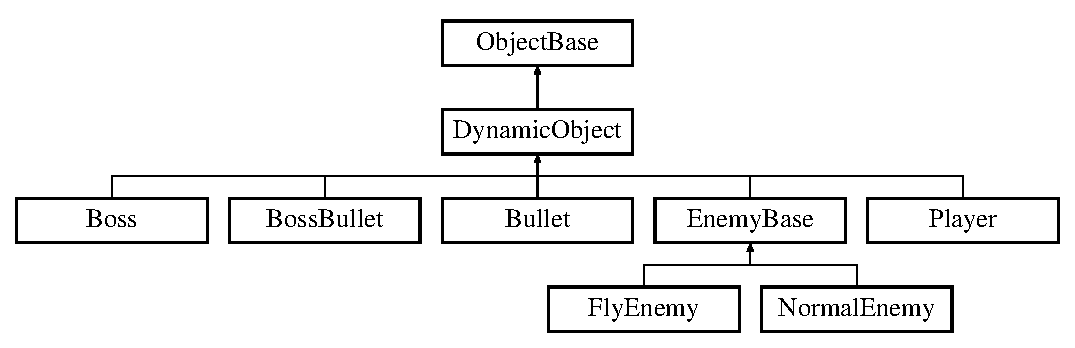
\includegraphics[height=4.000000cm]{class_dynamic_object}
\end{center}
\end{figure}
\subsection*{公開メンバ関数}
\begin{DoxyCompactItemize}
\item 
\mbox{\hyperlink{class_dynamic_object_a50a7adf3d7d1f411ed2aa9a663bfe275}{Dynamic\+Object}} ()
\begin{DoxyCompactList}\small\item\em コンストラクタ \end{DoxyCompactList}\item 
\mbox{\hyperlink{class_dynamic_object}{Dynamic\+Object}} \& \mbox{\hyperlink{class_dynamic_object_a3fed8d7c31826cc2f92fcd788a2feeb8}{operator=}} (const \mbox{\hyperlink{class_dynamic_object}{Dynamic\+Object}} \&other)
\begin{DoxyCompactList}\small\item\em コピー代入演算子 \end{DoxyCompactList}\item 
virtual \mbox{\hyperlink{class_dynamic_object_af9141dddf35d338d5bae491cb0455583}{$\sim$\+Dynamic\+Object}} ()
\end{DoxyCompactItemize}
\subsection*{限定公開メンバ関数}
\begin{DoxyCompactItemize}
\item 
virtual void \mbox{\hyperlink{class_dynamic_object_aa7488e1b4dfd7049447535d93d9d6783}{Render\+Process}} (bool)
\begin{DoxyCompactList}\small\item\em 描画 \end{DoxyCompactList}\end{DoxyCompactItemize}
\subsection*{その他の継承メンバ}


\subsection{詳解}
動くオブジェクトのスーパークラス 

\subsection{構築子と解体子}
\mbox{\Hypertarget{class_dynamic_object_a50a7adf3d7d1f411ed2aa9a663bfe275}\label{class_dynamic_object_a50a7adf3d7d1f411ed2aa9a663bfe275}} 
\index{Dynamic\+Object@{Dynamic\+Object}!Dynamic\+Object@{Dynamic\+Object}}
\index{Dynamic\+Object@{Dynamic\+Object}!Dynamic\+Object@{Dynamic\+Object}}
\subsubsection{\texorpdfstring{Dynamic\+Object()}{DynamicObject()}}
{\footnotesize\ttfamily Dynamic\+Object\+::\+Dynamic\+Object (\begin{DoxyParamCaption}{ }\end{DoxyParamCaption})\hspace{0.3cm}{\ttfamily [inline]}}



コンストラクタ 

\mbox{\Hypertarget{class_dynamic_object_af9141dddf35d338d5bae491cb0455583}\label{class_dynamic_object_af9141dddf35d338d5bae491cb0455583}} 
\index{Dynamic\+Object@{Dynamic\+Object}!````~Dynamic\+Object@{$\sim$\+Dynamic\+Object}}
\index{````~Dynamic\+Object@{$\sim$\+Dynamic\+Object}!Dynamic\+Object@{Dynamic\+Object}}
\subsubsection{\texorpdfstring{$\sim$\+Dynamic\+Object()}{~DynamicObject()}}
{\footnotesize\ttfamily virtual Dynamic\+Object\+::$\sim$\+Dynamic\+Object (\begin{DoxyParamCaption}{ }\end{DoxyParamCaption})\hspace{0.3cm}{\ttfamily [inline]}, {\ttfamily [virtual]}}



\subsection{関数詳解}
\mbox{\Hypertarget{class_dynamic_object_a3fed8d7c31826cc2f92fcd788a2feeb8}\label{class_dynamic_object_a3fed8d7c31826cc2f92fcd788a2feeb8}} 
\index{Dynamic\+Object@{Dynamic\+Object}!operator=@{operator=}}
\index{operator=@{operator=}!Dynamic\+Object@{Dynamic\+Object}}
\subsubsection{\texorpdfstring{operator=()}{operator=()}}
{\footnotesize\ttfamily \mbox{\hyperlink{class_dynamic_object}{Dynamic\+Object}}\& Dynamic\+Object\+::operator= (\begin{DoxyParamCaption}\item[{const \mbox{\hyperlink{class_dynamic_object}{Dynamic\+Object}} \&}]{other }\end{DoxyParamCaption})\hspace{0.3cm}{\ttfamily [inline]}}



コピー代入演算子 

\mbox{\Hypertarget{class_dynamic_object_aa7488e1b4dfd7049447535d93d9d6783}\label{class_dynamic_object_aa7488e1b4dfd7049447535d93d9d6783}} 
\index{Dynamic\+Object@{Dynamic\+Object}!Render\+Process@{Render\+Process}}
\index{Render\+Process@{Render\+Process}!Dynamic\+Object@{Dynamic\+Object}}
\subsubsection{\texorpdfstring{Render\+Process()}{RenderProcess()}}
{\footnotesize\ttfamily void Dynamic\+Object\+::\+Render\+Process (\begin{DoxyParamCaption}\item[{bool}]{camera\+\_\+affected }\end{DoxyParamCaption})\hspace{0.3cm}{\ttfamily [protected]}, {\ttfamily [virtual]}}



描画 


\begin{DoxyParams}{引数}
{\em camera\+\_\+affected} & カメラの位置によって位置を変えるかどうか \\
\hline
\end{DoxyParams}


\mbox{\hyperlink{class_object_base_aeac51d868beeb7f7fe900407b76b93a2}{Object\+Base}}を実装しています。



\mbox{\hyperlink{class_player_a8ac2e54fe5672d32186456b9735c02c3}{Player}}, \mbox{\hyperlink{class_boss_a6681bd6fc6dc35e200f9e63f196301af}{Boss}}, \mbox{\hyperlink{class_enemy_base_af874ce6fc410fddc7d55ffd7c7bedac8}{Enemy\+Base}}で再実装されています。



このクラス詳解は次のファイルから抽出されました\+:\begin{DoxyCompactItemize}
\item 
C\+:/\+Users/tokir/\+Documents/\+Git\+Hub/\+Weapon\+Merchant\+Adventure/src/src/object/base/dynamic/\mbox{\hyperlink{dynamic__object_8h}{dynamic\+\_\+object.\+h}}\item 
C\+:/\+Users/tokir/\+Documents/\+Git\+Hub/\+Weapon\+Merchant\+Adventure/src/src/object/base/dynamic/\mbox{\hyperlink{dynamic__object_8cpp}{dynamic\+\_\+object.\+cpp}}\end{DoxyCompactItemize}

\hypertarget{class_effect}{}\section{Effect クラス}
\label{class_effect}\index{Effect@{Effect}}


{\ttfamily \#include $<$effect.\+h$>$}

\subsection*{公開メンバ関数}
\begin{DoxyCompactItemize}
\item 
void \mbox{\hyperlink{class_effect_acedbf09deb825d561ab406a84b64faf3}{Init}} (std\+::string, W\+C\+H\+AR $\ast$, const float, const float)
\item 
void \mbox{\hyperlink{class_effect_a382a3189eb3a9fd9fbd9edf80c661225}{Set\+Param}} (const size\+\_\+t, const size\+\_\+t, const float)
\item 
void \mbox{\hyperlink{class_effect_a8a2e4b2b5c71a95ed864f4fd64b10343}{Start}} (const \mbox{\hyperlink{common_8h_ab1cb35b3a17c398d8ef71d5f779808bf}{Vec3}} \&)
\end{DoxyCompactItemize}
\subsection*{フレンド}
\begin{DoxyCompactItemize}
\item 
class \mbox{\hyperlink{class_effect_aa57a70c5d4b8abc800f69a1681448634}{Effect\+Manager}}
\end{DoxyCompactItemize}


\subsection{関数詳解}
\mbox{\Hypertarget{class_effect_acedbf09deb825d561ab406a84b64faf3}\label{class_effect_acedbf09deb825d561ab406a84b64faf3}} 
\index{Effect@{Effect}!Init@{Init}}
\index{Init@{Init}!Effect@{Effect}}
\subsubsection{\texorpdfstring{Init()}{Init()}}
{\footnotesize\ttfamily void Effect\+::\+Init (\begin{DoxyParamCaption}\item[{std\+::string}]{name,  }\item[{W\+C\+H\+AR $\ast$}]{path,  }\item[{const float}]{w,  }\item[{const float}]{h }\end{DoxyParamCaption})}

\mbox{\Hypertarget{class_effect_a382a3189eb3a9fd9fbd9edf80c661225}\label{class_effect_a382a3189eb3a9fd9fbd9edf80c661225}} 
\index{Effect@{Effect}!Set\+Param@{Set\+Param}}
\index{Set\+Param@{Set\+Param}!Effect@{Effect}}
\subsubsection{\texorpdfstring{Set\+Param()}{SetParam()}}
{\footnotesize\ttfamily void Effect\+::\+Set\+Param (\begin{DoxyParamCaption}\item[{const size\+\_\+t}]{n,  }\item[{const size\+\_\+t}]{life,  }\item[{const float}]{\+\_\+speed }\end{DoxyParamCaption})}

\mbox{\Hypertarget{class_effect_a8a2e4b2b5c71a95ed864f4fd64b10343}\label{class_effect_a8a2e4b2b5c71a95ed864f4fd64b10343}} 
\index{Effect@{Effect}!Start@{Start}}
\index{Start@{Start}!Effect@{Effect}}
\subsubsection{\texorpdfstring{Start()}{Start()}}
{\footnotesize\ttfamily void Effect\+::\+Start (\begin{DoxyParamCaption}\item[{const \mbox{\hyperlink{common_8h_ab1cb35b3a17c398d8ef71d5f779808bf}{Vec3}} \&}]{start }\end{DoxyParamCaption})}



\subsection{フレンドと関連関数の詳解}
\mbox{\Hypertarget{class_effect_aa57a70c5d4b8abc800f69a1681448634}\label{class_effect_aa57a70c5d4b8abc800f69a1681448634}} 
\index{Effect@{Effect}!Effect\+Manager@{Effect\+Manager}}
\index{Effect\+Manager@{Effect\+Manager}!Effect@{Effect}}
\subsubsection{\texorpdfstring{Effect\+Manager}{EffectManager}}
{\footnotesize\ttfamily friend class \mbox{\hyperlink{class_effect_manager}{Effect\+Manager}}\hspace{0.3cm}{\ttfamily [friend]}}



このクラス詳解は次のファイルから抽出されました\+:\begin{DoxyCompactItemize}
\item 
C\+:/\+Users/tokir/\+Documents/\+Git\+Hub/\+Weapon\+Merchant\+Adventure/src/src/effect/\mbox{\hyperlink{effect_8h}{effect.\+h}}\item 
C\+:/\+Users/tokir/\+Documents/\+Git\+Hub/\+Weapon\+Merchant\+Adventure/src/src/effect/\mbox{\hyperlink{effect_8cpp}{effect.\+cpp}}\end{DoxyCompactItemize}

\hypertarget{class_effect_manager}{}\section{Effect\+Manager クラス}
\label{class_effect_manager}\index{Effect\+Manager@{Effect\+Manager}}


{\ttfamily \#include $<$effect\+\_\+manager.\+h$>$}

Effect\+Manager の継承関係図\begin{figure}[H]
\begin{center}
\leavevmode
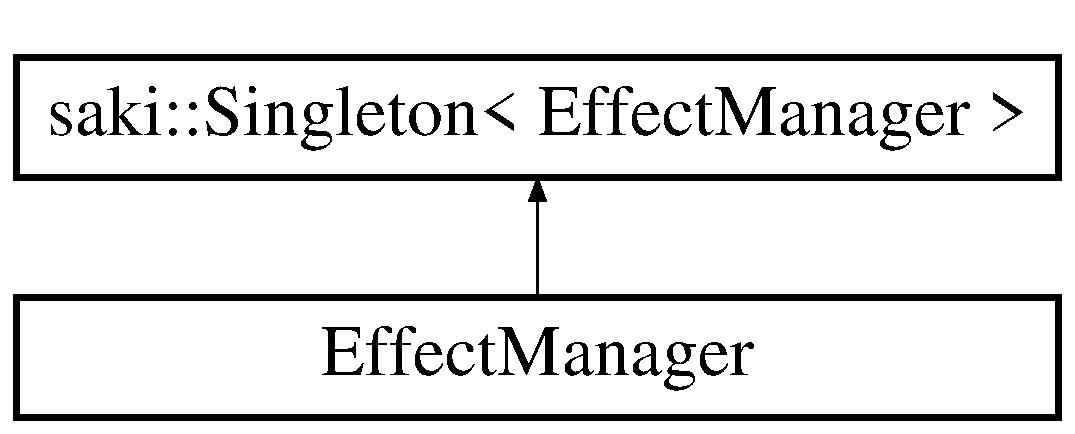
\includegraphics[height=2.000000cm]{class_effect_manager}
\end{center}
\end{figure}
\subsection*{公開メンバ関数}
\begin{DoxyCompactItemize}
\item 
void \mbox{\hyperlink{class_effect_manager_a427e9793802dce8d42a74723f44696fe}{Add\+Effect}} (const \mbox{\hyperlink{class_effect}{Effect}} \&)
\item 
void \mbox{\hyperlink{class_effect_manager_a966fbd56f3cf4763bc3a52fc5b8f4eff}{Update}} ()
\item 
void \mbox{\hyperlink{class_effect_manager_af5beef30ba12cb8c779b2c8d0ae55861}{Render}} ()
\item 
void \mbox{\hyperlink{class_effect_manager_a4efa9673f06df792679389b3c909bbc9}{Clear}} ()
\end{DoxyCompactItemize}
\subsection*{その他の継承メンバ}


\subsection{関数詳解}
\mbox{\Hypertarget{class_effect_manager_a427e9793802dce8d42a74723f44696fe}\label{class_effect_manager_a427e9793802dce8d42a74723f44696fe}} 
\index{Effect\+Manager@{Effect\+Manager}!Add\+Effect@{Add\+Effect}}
\index{Add\+Effect@{Add\+Effect}!Effect\+Manager@{Effect\+Manager}}
\subsubsection{\texorpdfstring{Add\+Effect()}{AddEffect()}}
{\footnotesize\ttfamily void Effect\+Manager\+::\+Add\+Effect (\begin{DoxyParamCaption}\item[{const \mbox{\hyperlink{class_effect}{Effect}} \&}]{effect }\end{DoxyParamCaption})}

\mbox{\Hypertarget{class_effect_manager_a4efa9673f06df792679389b3c909bbc9}\label{class_effect_manager_a4efa9673f06df792679389b3c909bbc9}} 
\index{Effect\+Manager@{Effect\+Manager}!Clear@{Clear}}
\index{Clear@{Clear}!Effect\+Manager@{Effect\+Manager}}
\subsubsection{\texorpdfstring{Clear()}{Clear()}}
{\footnotesize\ttfamily void Effect\+Manager\+::\+Clear (\begin{DoxyParamCaption}{ }\end{DoxyParamCaption})}

\mbox{\Hypertarget{class_effect_manager_af5beef30ba12cb8c779b2c8d0ae55861}\label{class_effect_manager_af5beef30ba12cb8c779b2c8d0ae55861}} 
\index{Effect\+Manager@{Effect\+Manager}!Render@{Render}}
\index{Render@{Render}!Effect\+Manager@{Effect\+Manager}}
\subsubsection{\texorpdfstring{Render()}{Render()}}
{\footnotesize\ttfamily void Effect\+Manager\+::\+Render (\begin{DoxyParamCaption}{ }\end{DoxyParamCaption})}

\mbox{\Hypertarget{class_effect_manager_a966fbd56f3cf4763bc3a52fc5b8f4eff}\label{class_effect_manager_a966fbd56f3cf4763bc3a52fc5b8f4eff}} 
\index{Effect\+Manager@{Effect\+Manager}!Update@{Update}}
\index{Update@{Update}!Effect\+Manager@{Effect\+Manager}}
\subsubsection{\texorpdfstring{Update()}{Update()}}
{\footnotesize\ttfamily void Effect\+Manager\+::\+Update (\begin{DoxyParamCaption}{ }\end{DoxyParamCaption})}



このクラス詳解は次のファイルから抽出されました\+:\begin{DoxyCompactItemize}
\item 
C\+:/\+Users/tokir/\+Documents/\+Git\+Hub/\+Weapon\+Merchant\+Adventure/src/src/effect/manager/\mbox{\hyperlink{effect__manager_8h}{effect\+\_\+manager.\+h}}\item 
C\+:/\+Users/tokir/\+Documents/\+Git\+Hub/\+Weapon\+Merchant\+Adventure/src/src/effect/manager/\mbox{\hyperlink{effect__manager_8cpp}{effect\+\_\+manager.\+cpp}}\end{DoxyCompactItemize}

\hypertarget{class_enemy_base}{}\section{Enemy\+Base クラス}
\label{class_enemy_base}\index{Enemy\+Base@{Enemy\+Base}}


エネミーのスーパークラス  




{\ttfamily \#include $<$enemy\+\_\+base.\+h$>$}

Enemy\+Base の継承関係図\begin{figure}[H]
\begin{center}
\leavevmode
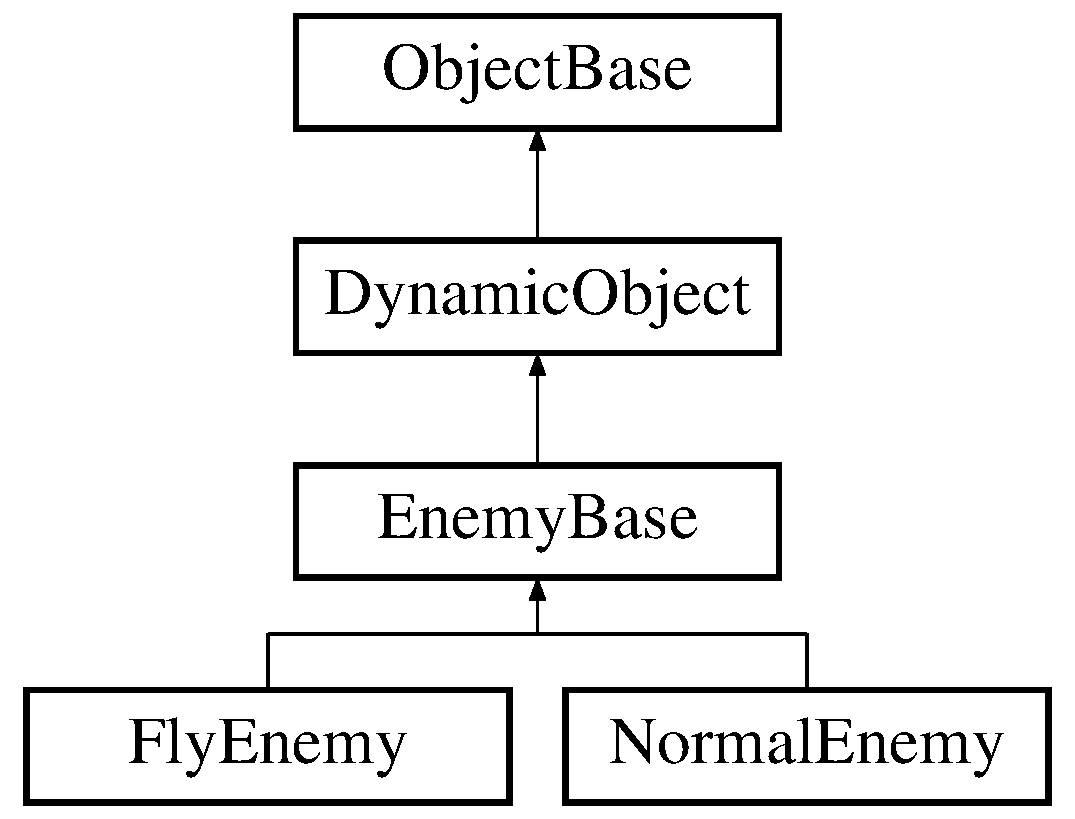
\includegraphics[height=4.000000cm]{class_enemy_base}
\end{center}
\end{figure}
\subsection*{公開メンバ関数}
\begin{DoxyCompactItemize}
\item 
\mbox{\hyperlink{class_enemy_base_abe56e3aa221224c1196fd65f897d5f19}{Enemy\+Base}} (\mbox{\hyperlink{enemy__base_8h_aef73e23ea1cdc9dda520bbb81af707db}{E\+N\+E\+M\+Y\+\_\+\+T\+Y\+PE}} et)
\begin{DoxyCompactList}\small\item\em コンストラクタ \end{DoxyCompactList}\item 
\mbox{\hyperlink{class_enemy_base}{Enemy\+Base}} \& \mbox{\hyperlink{class_enemy_base_ab733c603aedea1306fe42755c784a9db}{operator=}} (const \mbox{\hyperlink{class_enemy_base}{Enemy\+Base}} \&other)
\begin{DoxyCompactList}\small\item\em コピー代入演算子 \end{DoxyCompactList}\end{DoxyCompactItemize}
\subsection*{公開変数類}
\begin{DoxyCompactItemize}
\item 
\mbox{\hyperlink{enemy__base_8h_aef73e23ea1cdc9dda520bbb81af707db}{E\+N\+E\+M\+Y\+\_\+\+T\+Y\+PE}} \mbox{\hyperlink{class_enemy_base_a34ad22e6b0d06b8d63c207c843383eba}{enemy\+\_\+type}}
\end{DoxyCompactItemize}
\subsection*{限定公開メンバ関数}
\begin{DoxyCompactItemize}
\item 
void \mbox{\hyperlink{class_enemy_base_af874ce6fc410fddc7d55ffd7c7bedac8}{Render\+Process}} (bool) final
\begin{DoxyCompactList}\small\item\em 描画 \end{DoxyCompactList}\end{DoxyCompactItemize}
\subsection*{限定公開変数類}
\begin{DoxyCompactItemize}
\item 
\mbox{\hyperlink{class_square_collider}{Square\+Collider}} \mbox{\hyperlink{class_enemy_base_aea91f1e50b8977daa467a3d9fe5f0ef9}{collider}}
\item 
bool \mbox{\hyperlink{class_enemy_base_a0ea15efab9eed801fb676b9276c8e9c9}{destroy\+\_\+flg}} = false
\end{DoxyCompactItemize}


\subsection{詳解}
エネミーのスーパークラス 

\subsection{構築子と解体子}
\mbox{\Hypertarget{class_enemy_base_abe56e3aa221224c1196fd65f897d5f19}\label{class_enemy_base_abe56e3aa221224c1196fd65f897d5f19}} 
\index{Enemy\+Base@{Enemy\+Base}!Enemy\+Base@{Enemy\+Base}}
\index{Enemy\+Base@{Enemy\+Base}!Enemy\+Base@{Enemy\+Base}}
\subsubsection{\texorpdfstring{Enemy\+Base()}{EnemyBase()}}
{\footnotesize\ttfamily Enemy\+Base\+::\+Enemy\+Base (\begin{DoxyParamCaption}\item[{\mbox{\hyperlink{enemy__base_8h_aef73e23ea1cdc9dda520bbb81af707db}{E\+N\+E\+M\+Y\+\_\+\+T\+Y\+PE}}}]{et }\end{DoxyParamCaption})\hspace{0.3cm}{\ttfamily [inline]}}



コンストラクタ 


\begin{DoxyParams}{引数}
{\em et} & 敵のタイプ \\
\hline
\end{DoxyParams}


\subsection{関数詳解}
\mbox{\Hypertarget{class_enemy_base_ab733c603aedea1306fe42755c784a9db}\label{class_enemy_base_ab733c603aedea1306fe42755c784a9db}} 
\index{Enemy\+Base@{Enemy\+Base}!operator=@{operator=}}
\index{operator=@{operator=}!Enemy\+Base@{Enemy\+Base}}
\subsubsection{\texorpdfstring{operator=()}{operator=()}}
{\footnotesize\ttfamily \mbox{\hyperlink{class_enemy_base}{Enemy\+Base}}\& Enemy\+Base\+::operator= (\begin{DoxyParamCaption}\item[{const \mbox{\hyperlink{class_enemy_base}{Enemy\+Base}} \&}]{other }\end{DoxyParamCaption})\hspace{0.3cm}{\ttfamily [inline]}}



コピー代入演算子 

\mbox{\Hypertarget{class_enemy_base_af874ce6fc410fddc7d55ffd7c7bedac8}\label{class_enemy_base_af874ce6fc410fddc7d55ffd7c7bedac8}} 
\index{Enemy\+Base@{Enemy\+Base}!Render\+Process@{Render\+Process}}
\index{Render\+Process@{Render\+Process}!Enemy\+Base@{Enemy\+Base}}
\subsubsection{\texorpdfstring{Render\+Process()}{RenderProcess()}}
{\footnotesize\ttfamily void Enemy\+Base\+::\+Render\+Process (\begin{DoxyParamCaption}\item[{bool}]{camera\+\_\+affected }\end{DoxyParamCaption})\hspace{0.3cm}{\ttfamily [final]}, {\ttfamily [protected]}, {\ttfamily [virtual]}}



描画 


\begin{DoxyParams}{引数}
{\em camera\+\_\+affected} & カメラの位置によって描画する位置を変えるかどうか \\
\hline
\end{DoxyParams}


\mbox{\hyperlink{class_dynamic_object_aa7488e1b4dfd7049447535d93d9d6783}{Dynamic\+Object}}を再実装しています。



\subsection{メンバ詳解}
\mbox{\Hypertarget{class_enemy_base_aea91f1e50b8977daa467a3d9fe5f0ef9}\label{class_enemy_base_aea91f1e50b8977daa467a3d9fe5f0ef9}} 
\index{Enemy\+Base@{Enemy\+Base}!collider@{collider}}
\index{collider@{collider}!Enemy\+Base@{Enemy\+Base}}
\subsubsection{\texorpdfstring{collider}{collider}}
{\footnotesize\ttfamily \mbox{\hyperlink{class_square_collider}{Square\+Collider}} Enemy\+Base\+::collider\hspace{0.3cm}{\ttfamily [protected]}}

\mbox{\Hypertarget{class_enemy_base_a0ea15efab9eed801fb676b9276c8e9c9}\label{class_enemy_base_a0ea15efab9eed801fb676b9276c8e9c9}} 
\index{Enemy\+Base@{Enemy\+Base}!destroy\+\_\+flg@{destroy\+\_\+flg}}
\index{destroy\+\_\+flg@{destroy\+\_\+flg}!Enemy\+Base@{Enemy\+Base}}
\subsubsection{\texorpdfstring{destroy\+\_\+flg}{destroy\_flg}}
{\footnotesize\ttfamily bool Enemy\+Base\+::destroy\+\_\+flg = false\hspace{0.3cm}{\ttfamily [protected]}}

\mbox{\Hypertarget{class_enemy_base_a34ad22e6b0d06b8d63c207c843383eba}\label{class_enemy_base_a34ad22e6b0d06b8d63c207c843383eba}} 
\index{Enemy\+Base@{Enemy\+Base}!enemy\+\_\+type@{enemy\+\_\+type}}
\index{enemy\+\_\+type@{enemy\+\_\+type}!Enemy\+Base@{Enemy\+Base}}
\subsubsection{\texorpdfstring{enemy\+\_\+type}{enemy\_type}}
{\footnotesize\ttfamily \mbox{\hyperlink{enemy__base_8h_aef73e23ea1cdc9dda520bbb81af707db}{E\+N\+E\+M\+Y\+\_\+\+T\+Y\+PE}} Enemy\+Base\+::enemy\+\_\+type}



このクラス詳解は次のファイルから抽出されました\+:\begin{DoxyCompactItemize}
\item 
C\+:/\+Users/tokir/\+Documents/\+Git\+Hub/\+Weapon\+Merchant\+Adventure/src/src/object/character/enemy/base/\mbox{\hyperlink{enemy__base_8h}{enemy\+\_\+base.\+h}}\item 
C\+:/\+Users/tokir/\+Documents/\+Git\+Hub/\+Weapon\+Merchant\+Adventure/src/src/object/character/enemy/base/\mbox{\hyperlink{enemy__base_8cpp}{enemy\+\_\+base.\+cpp}}\end{DoxyCompactItemize}

\hypertarget{class_exit_scene}{}\section{Exit\+Scene クラス}
\label{class_exit_scene}\index{Exit\+Scene@{Exit\+Scene}}


{\ttfamily \#include $<$exit\+\_\+scene.\+h$>$}

Exit\+Scene の継承関係図\begin{figure}[H]
\begin{center}
\leavevmode
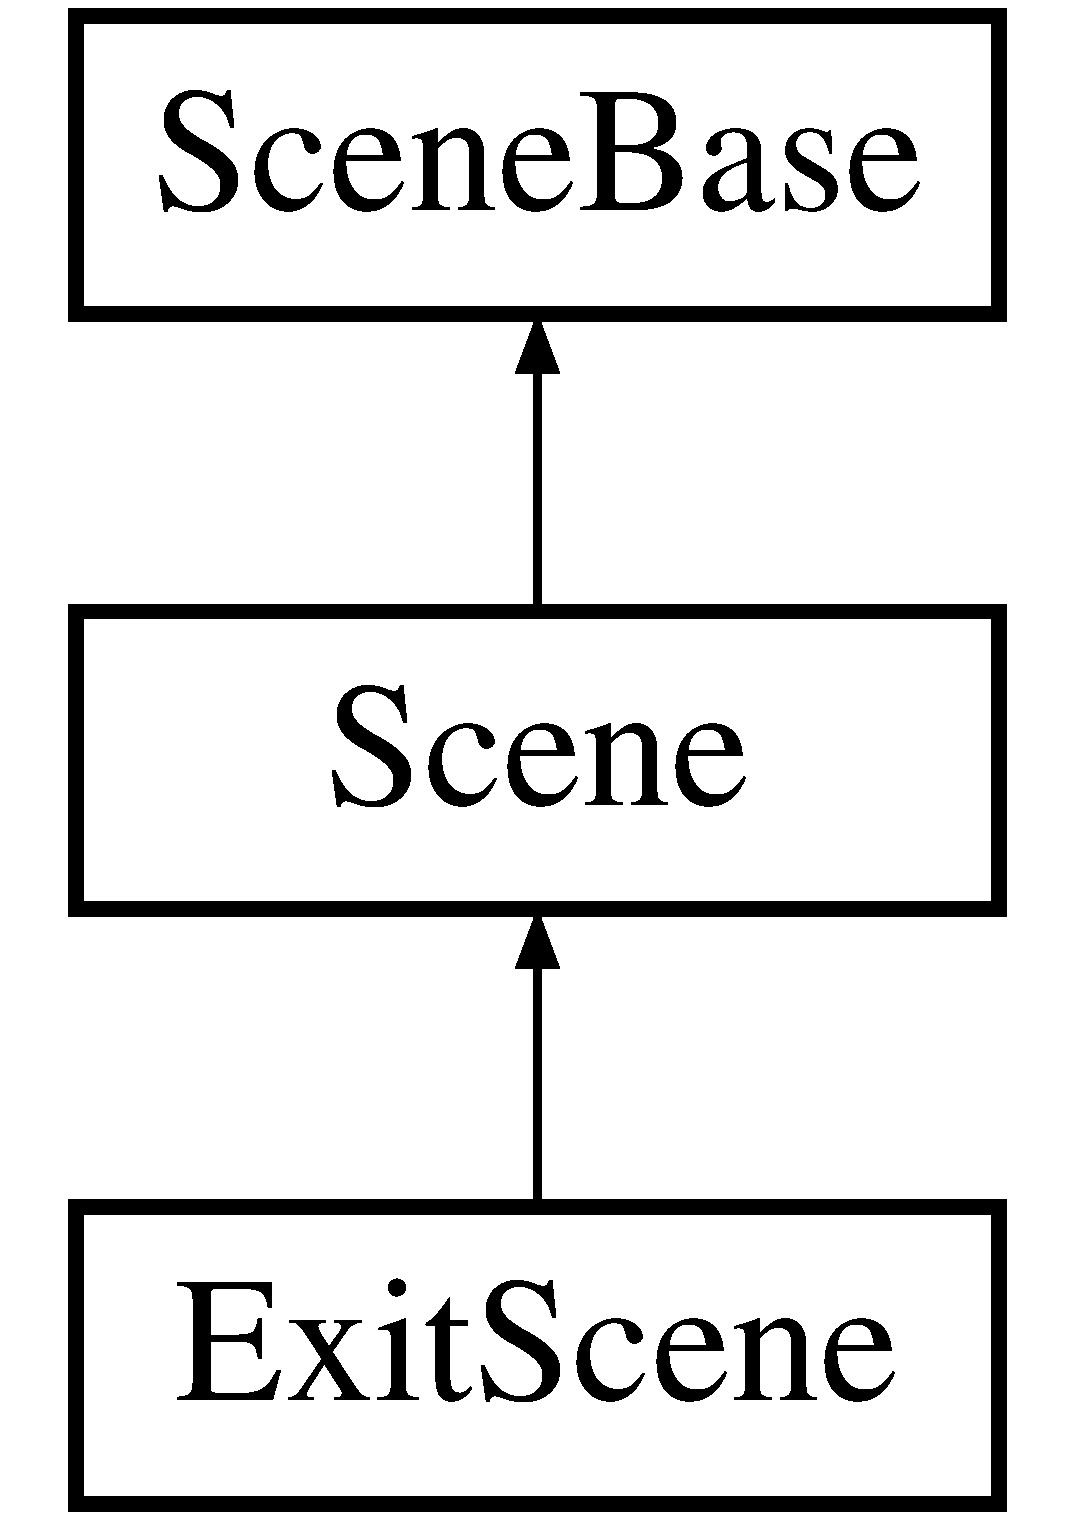
\includegraphics[height=3.000000cm]{class_exit_scene}
\end{center}
\end{figure}
\subsection*{公開メンバ関数}
\begin{DoxyCompactItemize}
\item 
void \mbox{\hyperlink{class_exit_scene_a10f6018b0c4c639d0e8756885dbc834c}{Init}} () final
\item 
std\+::shared\+\_\+ptr$<$ \mbox{\hyperlink{class_scene}{Scene}} $>$ \mbox{\hyperlink{class_exit_scene_a18655f3124150a911f266e66e3fc4480}{Update}} (std\+::shared\+\_\+ptr$<$ \mbox{\hyperlink{class_scene}{Scene}} $>$ \&p) final
\item 
void \mbox{\hyperlink{class_exit_scene_aecf5de52db863695794ee0b0e68a4ad0}{Render}} () final
\item 
void \mbox{\hyperlink{class_exit_scene_afc24a09da4a553109f813566f5d04da8}{Destroy}} () final
\end{DoxyCompactItemize}


\subsection{関数詳解}
\mbox{\Hypertarget{class_exit_scene_afc24a09da4a553109f813566f5d04da8}\label{class_exit_scene_afc24a09da4a553109f813566f5d04da8}} 
\index{Exit\+Scene@{Exit\+Scene}!Destroy@{Destroy}}
\index{Destroy@{Destroy}!Exit\+Scene@{Exit\+Scene}}
\subsubsection{\texorpdfstring{Destroy()}{Destroy()}}
{\footnotesize\ttfamily void Exit\+Scene\+::\+Destroy (\begin{DoxyParamCaption}{ }\end{DoxyParamCaption})\hspace{0.3cm}{\ttfamily [inline]}, {\ttfamily [final]}, {\ttfamily [virtual]}}



\mbox{\hyperlink{class_scene_base_a7c5b54020bc519b4dadfe9770d6b27f7}{Scene\+Base}}を実装しています。

\mbox{\Hypertarget{class_exit_scene_a10f6018b0c4c639d0e8756885dbc834c}\label{class_exit_scene_a10f6018b0c4c639d0e8756885dbc834c}} 
\index{Exit\+Scene@{Exit\+Scene}!Init@{Init}}
\index{Init@{Init}!Exit\+Scene@{Exit\+Scene}}
\subsubsection{\texorpdfstring{Init()}{Init()}}
{\footnotesize\ttfamily void Exit\+Scene\+::\+Init (\begin{DoxyParamCaption}{ }\end{DoxyParamCaption})\hspace{0.3cm}{\ttfamily [inline]}, {\ttfamily [final]}, {\ttfamily [virtual]}}



\mbox{\hyperlink{class_scene_base_a24d7db43c819924dc8b07b436f6d3148}{Scene\+Base}}を実装しています。

\mbox{\Hypertarget{class_exit_scene_aecf5de52db863695794ee0b0e68a4ad0}\label{class_exit_scene_aecf5de52db863695794ee0b0e68a4ad0}} 
\index{Exit\+Scene@{Exit\+Scene}!Render@{Render}}
\index{Render@{Render}!Exit\+Scene@{Exit\+Scene}}
\subsubsection{\texorpdfstring{Render()}{Render()}}
{\footnotesize\ttfamily void Exit\+Scene\+::\+Render (\begin{DoxyParamCaption}{ }\end{DoxyParamCaption})\hspace{0.3cm}{\ttfamily [inline]}, {\ttfamily [final]}, {\ttfamily [virtual]}}



\mbox{\hyperlink{class_scene_base_ad981674ce731ea267f398e889bbb9dc3}{Scene\+Base}}を実装しています。

\mbox{\Hypertarget{class_exit_scene_a18655f3124150a911f266e66e3fc4480}\label{class_exit_scene_a18655f3124150a911f266e66e3fc4480}} 
\index{Exit\+Scene@{Exit\+Scene}!Update@{Update}}
\index{Update@{Update}!Exit\+Scene@{Exit\+Scene}}
\subsubsection{\texorpdfstring{Update()}{Update()}}
{\footnotesize\ttfamily std\+::shared\+\_\+ptr$<$\mbox{\hyperlink{class_scene}{Scene}}$>$ Exit\+Scene\+::\+Update (\begin{DoxyParamCaption}\item[{std\+::shared\+\_\+ptr$<$ \mbox{\hyperlink{class_scene}{Scene}} $>$ \&}]{p }\end{DoxyParamCaption})\hspace{0.3cm}{\ttfamily [inline]}, {\ttfamily [final]}, {\ttfamily [virtual]}}



\mbox{\hyperlink{class_scene_ab71ee5f19764b90c87b4574aa1cb1d25}{Scene}}を実装しています。



このクラス詳解は次のファイルから抽出されました\+:\begin{DoxyCompactItemize}
\item 
C\+:/\+Users/tokir/\+Documents/\+Git\+Hub/\+Weapon\+Merchant\+Adventure/src/src/scene/\mbox{\hyperlink{exit__scene_8h}{exit\+\_\+scene.\+h}}\end{DoxyCompactItemize}

\hypertarget{class_fade}{}\section{Fade クラス}
\label{class_fade}\index{Fade@{Fade}}


フェードクラス  




{\ttfamily \#include $<$fade.\+h$>$}

Fade の継承関係図\begin{figure}[H]
\begin{center}
\leavevmode
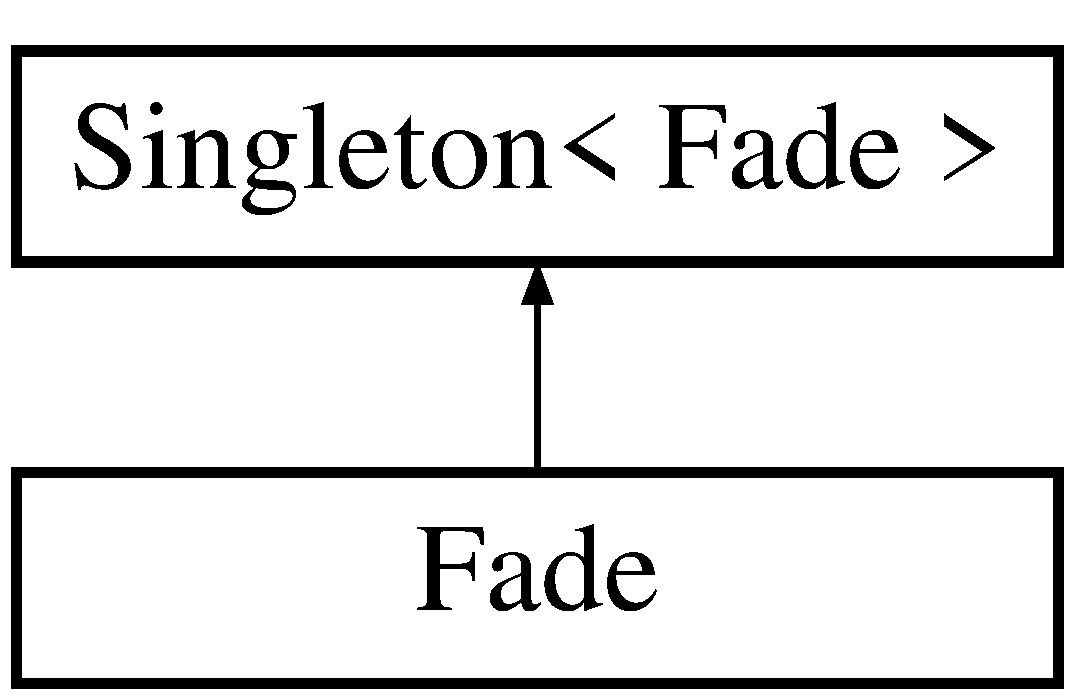
\includegraphics[height=2.000000cm]{class_fade}
\end{center}
\end{figure}
\subsection*{公開メンバ関数}
\begin{DoxyCompactItemize}
\item 
void \mbox{\hyperlink{class_fade_ac2a47819e1390abcae3259bcb42bddf5}{Init}} ()
\begin{DoxyCompactList}\small\item\em 初期化 \end{DoxyCompactList}\item 
bool \mbox{\hyperlink{class_fade_aaf97d1ac502c86612a97fde0e2fbf308}{Update}} (const bool)
\begin{DoxyCompactList}\small\item\em 更新 \end{DoxyCompactList}\item 
void \mbox{\hyperlink{class_fade_abfe024be1a10d4849582adf58fe6682a}{Render}} ()
\begin{DoxyCompactList}\small\item\em 描画 \end{DoxyCompactList}\item 
void \mbox{\hyperlink{class_fade_afd5cce157c2876a800ea59b2648547c2}{Destroy}} ()
\begin{DoxyCompactList}\small\item\em 破棄 \end{DoxyCompactList}\end{DoxyCompactItemize}
\subsection*{その他の継承メンバ}


\subsection{詳解}
フェードクラス 

\subsection{関数詳解}
\mbox{\Hypertarget{class_fade_afd5cce157c2876a800ea59b2648547c2}\label{class_fade_afd5cce157c2876a800ea59b2648547c2}} 
\index{Fade@{Fade}!Destroy@{Destroy}}
\index{Destroy@{Destroy}!Fade@{Fade}}
\subsubsection{\texorpdfstring{Destroy()}{Destroy()}}
{\footnotesize\ttfamily void Fade\+::\+Destroy (\begin{DoxyParamCaption}{ }\end{DoxyParamCaption})}



破棄 

\mbox{\Hypertarget{class_fade_ac2a47819e1390abcae3259bcb42bddf5}\label{class_fade_ac2a47819e1390abcae3259bcb42bddf5}} 
\index{Fade@{Fade}!Init@{Init}}
\index{Init@{Init}!Fade@{Fade}}
\subsubsection{\texorpdfstring{Init()}{Init()}}
{\footnotesize\ttfamily void Fade\+::\+Init (\begin{DoxyParamCaption}{ }\end{DoxyParamCaption})}



初期化 

\mbox{\Hypertarget{class_fade_abfe024be1a10d4849582adf58fe6682a}\label{class_fade_abfe024be1a10d4849582adf58fe6682a}} 
\index{Fade@{Fade}!Render@{Render}}
\index{Render@{Render}!Fade@{Fade}}
\subsubsection{\texorpdfstring{Render()}{Render()}}
{\footnotesize\ttfamily void Fade\+::\+Render (\begin{DoxyParamCaption}{ }\end{DoxyParamCaption})}



描画 

\mbox{\Hypertarget{class_fade_aaf97d1ac502c86612a97fde0e2fbf308}\label{class_fade_aaf97d1ac502c86612a97fde0e2fbf308}} 
\index{Fade@{Fade}!Update@{Update}}
\index{Update@{Update}!Fade@{Fade}}
\subsubsection{\texorpdfstring{Update()}{Update()}}
{\footnotesize\ttfamily bool Fade\+::\+Update (\begin{DoxyParamCaption}\item[{const bool}]{fade\+\_\+in }\end{DoxyParamCaption})}



更新 


\begin{DoxyParams}{引数}
{\em fade\+\_\+in} & フェードインかどうか \\
\hline
\end{DoxyParams}
\begin{DoxyReturn}{戻り値}
bool フェードインかアウトが終わったらtrue 
\end{DoxyReturn}


このクラス詳解は次のファイルから抽出されました\+:\begin{DoxyCompactItemize}
\item 
C\+:/\+Users/tokir/\+Documents/\+Git\+Hub/\+Weapon\+Merchant\+Adventure/src/scene/fade/\mbox{\hyperlink{fade_8h}{fade.\+h}}\item 
C\+:/\+Users/tokir/\+Documents/\+Git\+Hub/\+Weapon\+Merchant\+Adventure/src/scene/fade/\mbox{\hyperlink{fade_8cpp}{fade.\+cpp}}\end{DoxyCompactItemize}

\hypertarget{class_fly_enemy}{}\section{Fly\+Enemy クラス}
\label{class_fly_enemy}\index{Fly\+Enemy@{Fly\+Enemy}}


飛ぶエネミークラス  




{\ttfamily \#include $<$fly\+\_\+enemy.\+h$>$}

Fly\+Enemy の継承関係図\begin{figure}[H]
\begin{center}
\leavevmode
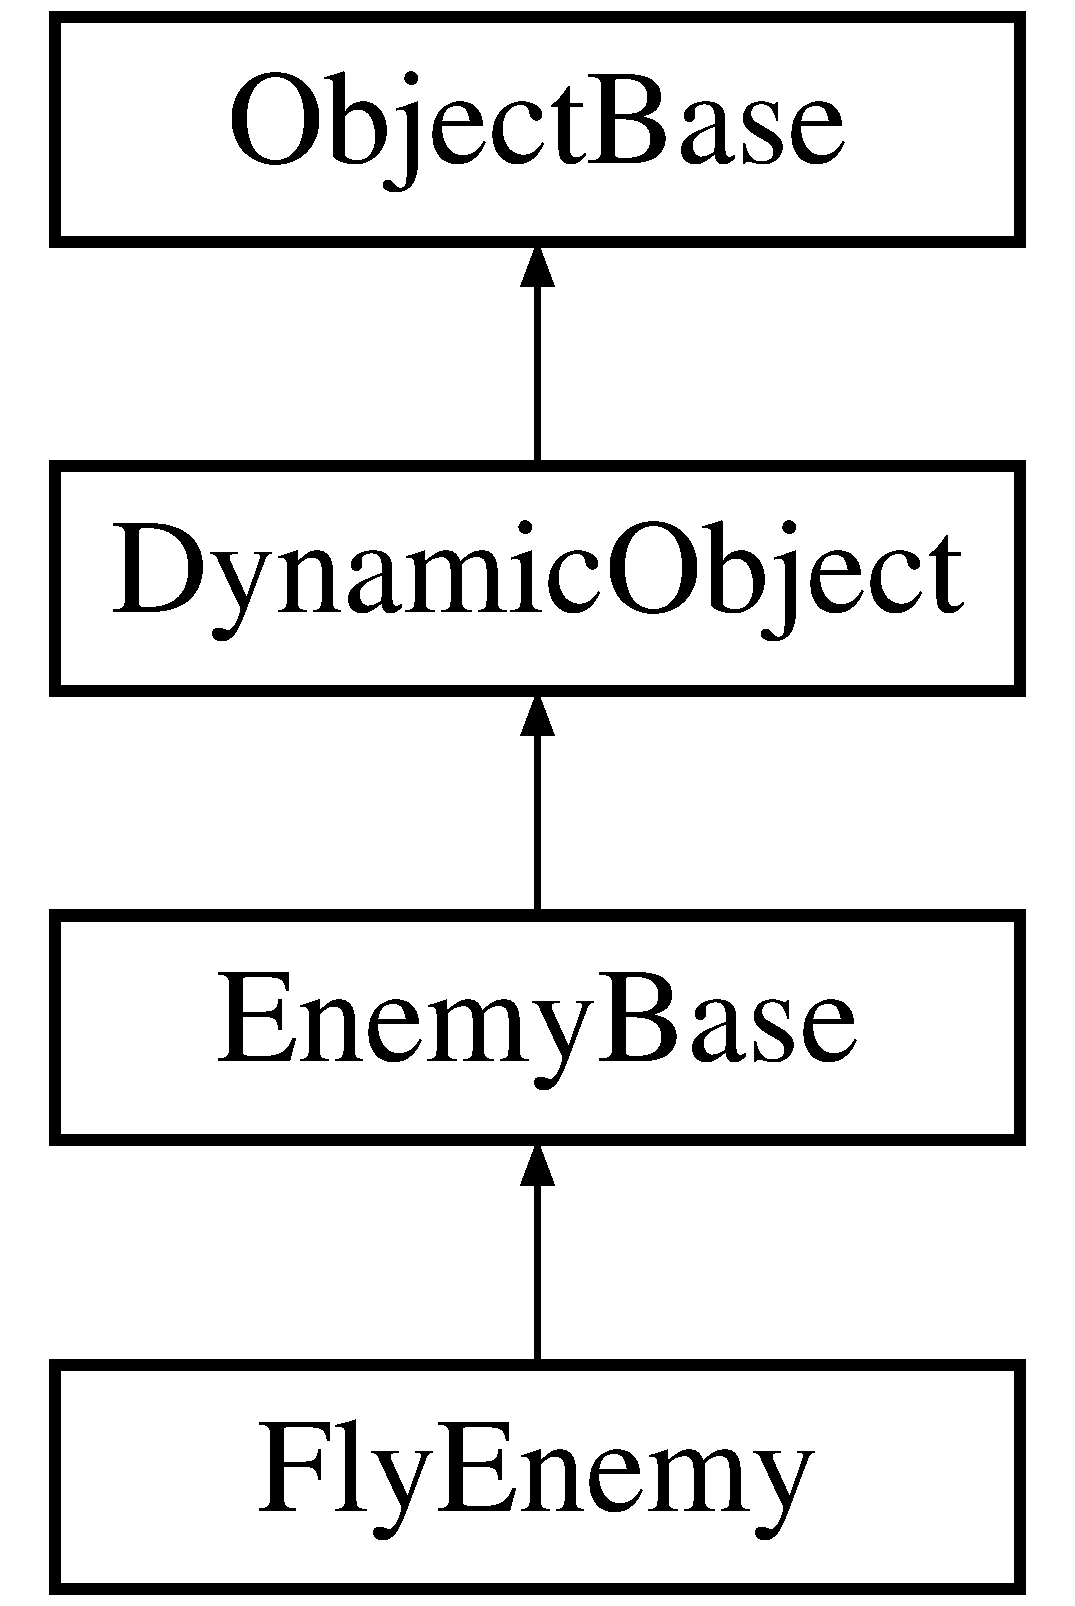
\includegraphics[height=4.000000cm]{class_fly_enemy}
\end{center}
\end{figure}
\subsection*{公開メンバ関数}
\begin{DoxyCompactItemize}
\item 
\mbox{\hyperlink{class_fly_enemy_a92bb66e1f877440afab15a36ffebd74d}{Fly\+Enemy}} ()
\begin{DoxyCompactList}\small\item\em コンストラクタ \end{DoxyCompactList}\item 
\mbox{\hyperlink{class_fly_enemy_af206898a5e1b59cc7bba2e4c13b72384}{Fly\+Enemy}} (const \mbox{\hyperlink{class_fly_enemy}{Fly\+Enemy}} \&ne)
\begin{DoxyCompactList}\small\item\em コピーコンストラクタ \end{DoxyCompactList}\item 
\mbox{\hyperlink{class_fly_enemy_ad32ad41958e55f3028b0beb068813bc1}{Fly\+Enemy}} (\mbox{\hyperlink{class_fly_enemy}{Fly\+Enemy}} \&\&ne)
\begin{DoxyCompactList}\small\item\em ムーブコンストラクタ \end{DoxyCompactList}\item 
\mbox{\hyperlink{class_fly_enemy}{Fly\+Enemy}} \& \mbox{\hyperlink{class_fly_enemy_a6cc3f3701b503020620c02667705fd23}{operator=}} (const \mbox{\hyperlink{class_fly_enemy}{Fly\+Enemy}} \&other)
\begin{DoxyCompactList}\small\item\em コピー代入演算子 \end{DoxyCompactList}\item 
void \mbox{\hyperlink{class_fly_enemy_adaabf7ce270104e30df29bfa464d72ce}{Collision}} (\mbox{\hyperlink{class_object_base}{Object\+Base}} $\ast$, \mbox{\hyperlink{common_8h_afb0c5e21d4133ff4f200992c0b534e1b}{V\+E\+C2}}) final
\begin{DoxyCompactList}\small\item\em 当たったときに実行する関数 \end{DoxyCompactList}\item 
void \mbox{\hyperlink{class_fly_enemy_af7ce5137e8eb2e8cc6654fbbdbc714cd}{Destroy}} () final
\begin{DoxyCompactList}\small\item\em 破棄 \end{DoxyCompactList}\item 
\mbox{\hyperlink{class_fly_enemy_ae4345f89a659b559c08d0bb879db7158}{$\sim$\+Fly\+Enemy}} ()
\begin{DoxyCompactList}\small\item\em デストラクタ \end{DoxyCompactList}\item 
void \mbox{\hyperlink{class_fly_enemy_a137e5a5f2adb7eacd282bbf662242cb3}{Set\+Move}} (const \mbox{\hyperlink{common_8h_afb0c5e21d4133ff4f200992c0b534e1b}{V\+E\+C2}} \&range, float time)
\begin{DoxyCompactList}\small\item\em 移動範囲を決める \end{DoxyCompactList}\end{DoxyCompactItemize}
\subsection*{限定公開メンバ関数}
\begin{DoxyCompactItemize}
\item 
void \mbox{\hyperlink{class_fly_enemy_afe4ddbf7089952146443f4ca71f55b13}{Init\+Process}} () final
\begin{DoxyCompactList}\small\item\em 初期化 \end{DoxyCompactList}\item 
void \mbox{\hyperlink{class_fly_enemy_a5122c8fea26ebbd0390acfd6e41931ff}{Update\+Process}} () final
\begin{DoxyCompactList}\small\item\em 更新 \end{DoxyCompactList}\end{DoxyCompactItemize}
\subsection*{その他の継承メンバ}


\subsection{詳解}
飛ぶエネミークラス 

\subsection{構築子と解体子}
\mbox{\Hypertarget{class_fly_enemy_a92bb66e1f877440afab15a36ffebd74d}\label{class_fly_enemy_a92bb66e1f877440afab15a36ffebd74d}} 
\index{Fly\+Enemy@{Fly\+Enemy}!Fly\+Enemy@{Fly\+Enemy}}
\index{Fly\+Enemy@{Fly\+Enemy}!Fly\+Enemy@{Fly\+Enemy}}
\subsubsection{\texorpdfstring{Fly\+Enemy()}{FlyEnemy()}\hspace{0.1cm}{\footnotesize\ttfamily [1/3]}}
{\footnotesize\ttfamily Fly\+Enemy\+::\+Fly\+Enemy (\begin{DoxyParamCaption}{ }\end{DoxyParamCaption})\hspace{0.3cm}{\ttfamily [inline]}}



コンストラクタ 

\mbox{\Hypertarget{class_fly_enemy_af206898a5e1b59cc7bba2e4c13b72384}\label{class_fly_enemy_af206898a5e1b59cc7bba2e4c13b72384}} 
\index{Fly\+Enemy@{Fly\+Enemy}!Fly\+Enemy@{Fly\+Enemy}}
\index{Fly\+Enemy@{Fly\+Enemy}!Fly\+Enemy@{Fly\+Enemy}}
\subsubsection{\texorpdfstring{Fly\+Enemy()}{FlyEnemy()}\hspace{0.1cm}{\footnotesize\ttfamily [2/3]}}
{\footnotesize\ttfamily Fly\+Enemy\+::\+Fly\+Enemy (\begin{DoxyParamCaption}\item[{const \mbox{\hyperlink{class_fly_enemy}{Fly\+Enemy}} \&}]{ne }\end{DoxyParamCaption})\hspace{0.3cm}{\ttfamily [inline]}}



コピーコンストラクタ 

\mbox{\Hypertarget{class_fly_enemy_ad32ad41958e55f3028b0beb068813bc1}\label{class_fly_enemy_ad32ad41958e55f3028b0beb068813bc1}} 
\index{Fly\+Enemy@{Fly\+Enemy}!Fly\+Enemy@{Fly\+Enemy}}
\index{Fly\+Enemy@{Fly\+Enemy}!Fly\+Enemy@{Fly\+Enemy}}
\subsubsection{\texorpdfstring{Fly\+Enemy()}{FlyEnemy()}\hspace{0.1cm}{\footnotesize\ttfamily [3/3]}}
{\footnotesize\ttfamily Fly\+Enemy\+::\+Fly\+Enemy (\begin{DoxyParamCaption}\item[{\mbox{\hyperlink{class_fly_enemy}{Fly\+Enemy}} \&\&}]{ne }\end{DoxyParamCaption})\hspace{0.3cm}{\ttfamily [inline]}}



ムーブコンストラクタ 

\mbox{\Hypertarget{class_fly_enemy_ae4345f89a659b559c08d0bb879db7158}\label{class_fly_enemy_ae4345f89a659b559c08d0bb879db7158}} 
\index{Fly\+Enemy@{Fly\+Enemy}!````~Fly\+Enemy@{$\sim$\+Fly\+Enemy}}
\index{````~Fly\+Enemy@{$\sim$\+Fly\+Enemy}!Fly\+Enemy@{Fly\+Enemy}}
\subsubsection{\texorpdfstring{$\sim$\+Fly\+Enemy()}{~FlyEnemy()}}
{\footnotesize\ttfamily Fly\+Enemy\+::$\sim$\+Fly\+Enemy (\begin{DoxyParamCaption}{ }\end{DoxyParamCaption})\hspace{0.3cm}{\ttfamily [inline]}}



デストラクタ 



\subsection{関数詳解}
\mbox{\Hypertarget{class_fly_enemy_adaabf7ce270104e30df29bfa464d72ce}\label{class_fly_enemy_adaabf7ce270104e30df29bfa464d72ce}} 
\index{Fly\+Enemy@{Fly\+Enemy}!Collision@{Collision}}
\index{Collision@{Collision}!Fly\+Enemy@{Fly\+Enemy}}
\subsubsection{\texorpdfstring{Collision()}{Collision()}}
{\footnotesize\ttfamily void Fly\+Enemy\+::\+Collision (\begin{DoxyParamCaption}\item[{\mbox{\hyperlink{class_object_base}{Object\+Base}} $\ast$}]{obj,  }\item[{\mbox{\hyperlink{common_8h_afb0c5e21d4133ff4f200992c0b534e1b}{V\+E\+C2}}}]{ }\end{DoxyParamCaption})\hspace{0.3cm}{\ttfamily [final]}, {\ttfamily [virtual]}}



当たったときに実行する関数 


\begin{DoxyParams}{引数}
{\em obj} & 当たった相手のオブジェクト \\
\hline
\end{DoxyParams}


\mbox{\hyperlink{class_object_base_ad772d7a42f5e46c39481f5db22ee8193}{Object\+Base}}を再実装しています。

\mbox{\Hypertarget{class_fly_enemy_af7ce5137e8eb2e8cc6654fbbdbc714cd}\label{class_fly_enemy_af7ce5137e8eb2e8cc6654fbbdbc714cd}} 
\index{Fly\+Enemy@{Fly\+Enemy}!Destroy@{Destroy}}
\index{Destroy@{Destroy}!Fly\+Enemy@{Fly\+Enemy}}
\subsubsection{\texorpdfstring{Destroy()}{Destroy()}}
{\footnotesize\ttfamily void Fly\+Enemy\+::\+Destroy (\begin{DoxyParamCaption}{ }\end{DoxyParamCaption})\hspace{0.3cm}{\ttfamily [final]}, {\ttfamily [virtual]}}



破棄 



\mbox{\hyperlink{class_object_base_a7fa4c548153c3af20f89673ffea809af}{Object\+Base}}を実装しています。

\mbox{\Hypertarget{class_fly_enemy_afe4ddbf7089952146443f4ca71f55b13}\label{class_fly_enemy_afe4ddbf7089952146443f4ca71f55b13}} 
\index{Fly\+Enemy@{Fly\+Enemy}!Init\+Process@{Init\+Process}}
\index{Init\+Process@{Init\+Process}!Fly\+Enemy@{Fly\+Enemy}}
\subsubsection{\texorpdfstring{Init\+Process()}{InitProcess()}}
{\footnotesize\ttfamily void Fly\+Enemy\+::\+Init\+Process (\begin{DoxyParamCaption}{ }\end{DoxyParamCaption})\hspace{0.3cm}{\ttfamily [final]}, {\ttfamily [protected]}, {\ttfamily [virtual]}}



初期化 



\mbox{\hyperlink{class_object_base_af133f36f2bca1dcfd962e2cfac61ab51}{Object\+Base}}を実装しています。

\mbox{\Hypertarget{class_fly_enemy_a6cc3f3701b503020620c02667705fd23}\label{class_fly_enemy_a6cc3f3701b503020620c02667705fd23}} 
\index{Fly\+Enemy@{Fly\+Enemy}!operator=@{operator=}}
\index{operator=@{operator=}!Fly\+Enemy@{Fly\+Enemy}}
\subsubsection{\texorpdfstring{operator=()}{operator=()}}
{\footnotesize\ttfamily \mbox{\hyperlink{class_fly_enemy}{Fly\+Enemy}}\& Fly\+Enemy\+::operator= (\begin{DoxyParamCaption}\item[{const \mbox{\hyperlink{class_fly_enemy}{Fly\+Enemy}} \&}]{other }\end{DoxyParamCaption})\hspace{0.3cm}{\ttfamily [inline]}}



コピー代入演算子 

\mbox{\Hypertarget{class_fly_enemy_a137e5a5f2adb7eacd282bbf662242cb3}\label{class_fly_enemy_a137e5a5f2adb7eacd282bbf662242cb3}} 
\index{Fly\+Enemy@{Fly\+Enemy}!Set\+Move@{Set\+Move}}
\index{Set\+Move@{Set\+Move}!Fly\+Enemy@{Fly\+Enemy}}
\subsubsection{\texorpdfstring{Set\+Move()}{SetMove()}}
{\footnotesize\ttfamily void Fly\+Enemy\+::\+Set\+Move (\begin{DoxyParamCaption}\item[{const \mbox{\hyperlink{common_8h_afb0c5e21d4133ff4f200992c0b534e1b}{V\+E\+C2}} \&}]{range,  }\item[{float}]{time }\end{DoxyParamCaption})\hspace{0.3cm}{\ttfamily [inline]}}



移動範囲を決める 


\begin{DoxyParams}{引数}
{\em range} & 現在の位置からどのくらい移動するか \\
\hline
{\em time} & どのくらいの時間をかけて行き来するか \\
\hline
\end{DoxyParams}
\mbox{\Hypertarget{class_fly_enemy_a5122c8fea26ebbd0390acfd6e41931ff}\label{class_fly_enemy_a5122c8fea26ebbd0390acfd6e41931ff}} 
\index{Fly\+Enemy@{Fly\+Enemy}!Update\+Process@{Update\+Process}}
\index{Update\+Process@{Update\+Process}!Fly\+Enemy@{Fly\+Enemy}}
\subsubsection{\texorpdfstring{Update\+Process()}{UpdateProcess()}}
{\footnotesize\ttfamily void Fly\+Enemy\+::\+Update\+Process (\begin{DoxyParamCaption}{ }\end{DoxyParamCaption})\hspace{0.3cm}{\ttfamily [final]}, {\ttfamily [protected]}, {\ttfamily [virtual]}}



更新 



\mbox{\hyperlink{class_object_base_a8b5b72b363a419767efde0b0e692ea95}{Object\+Base}}を実装しています。



このクラス詳解は次のファイルから抽出されました\+:\begin{DoxyCompactItemize}
\item 
C\+:/\+Users/tokir/\+Documents/\+Git\+Hub/\+Weapon\+Merchant\+Adventure/src/object/character/enemy/fly/\mbox{\hyperlink{fly__enemy_8h}{fly\+\_\+enemy.\+h}}\item 
C\+:/\+Users/tokir/\+Documents/\+Git\+Hub/\+Weapon\+Merchant\+Adventure/src/object/character/enemy/fly/\mbox{\hyperlink{fly__enemy_8cpp}{fly\+\_\+enemy.\+cpp}}\end{DoxyCompactItemize}

\hypertarget{class_game_over}{}\section{Game\+Over クラス}
\label{class_game_over}\index{Game\+Over@{Game\+Over}}


ゲームオーバークラス  




{\ttfamily \#include $<$game\+\_\+over.\+h$>$}

Game\+Over の継承関係図\begin{figure}[H]
\begin{center}
\leavevmode
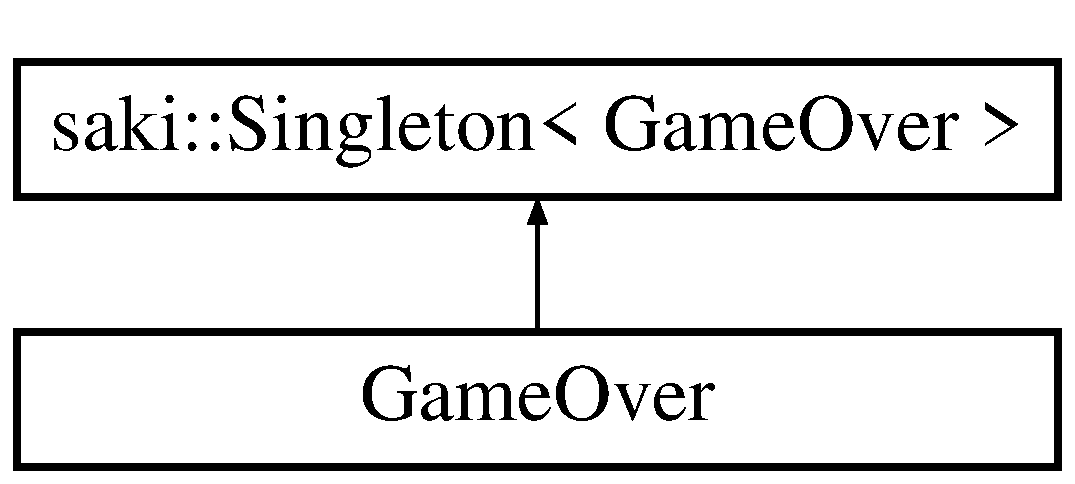
\includegraphics[height=2.000000cm]{class_game_over}
\end{center}
\end{figure}
\subsection*{公開メンバ関数}
\begin{DoxyCompactItemize}
\item 
void \mbox{\hyperlink{class_game_over_ac13d1bd0fe9f8db0ef0301c9ec63a9e0}{Init}} ()
\begin{DoxyCompactList}\small\item\em ゲームオーバーシーンの初期化 \end{DoxyCompactList}\item 
void \mbox{\hyperlink{class_game_over_afed8423e1fc3b76ba826b9c376913df9}{Reset}} ()
\begin{DoxyCompactList}\small\item\em 値をリセットする \end{DoxyCompactList}\item 
void \mbox{\hyperlink{class_game_over_ab5d86cf67969620b78fb6f978802daca}{Set\+Color}} ()
\begin{DoxyCompactList}\small\item\em フェード時に色をセットする \end{DoxyCompactList}\item 
void \mbox{\hyperlink{class_game_over_a13dd856f7d38020ad388cacda5fef575}{Update}} (std\+::shared\+\_\+ptr$<$ \mbox{\hyperlink{class_scene}{Scene}} $>$ \&, std\+::shared\+\_\+ptr$<$ \mbox{\hyperlink{class_scene}{Scene}} $>$ \&\&)
\begin{DoxyCompactList}\small\item\em ゲームオーバーシーンの更新 \end{DoxyCompactList}\item 
void \mbox{\hyperlink{class_game_over_ae16a875f25d87d8d368f24db4137f4c1}{Render}} ()
\begin{DoxyCompactList}\small\item\em ゲームオーバーシーンの描画 \end{DoxyCompactList}\end{DoxyCompactItemize}
\subsection*{公開変数類}
\begin{DoxyCompactItemize}
\item 
bool \mbox{\hyperlink{class_game_over_a7de925db0f485b924ef29f4649d2984d}{game\+\_\+over\+\_\+flg}} = false
\end{DoxyCompactItemize}
\subsection*{その他の継承メンバ}


\subsection{詳解}
ゲームオーバークラス 

\subsection{関数詳解}
\mbox{\Hypertarget{class_game_over_ac13d1bd0fe9f8db0ef0301c9ec63a9e0}\label{class_game_over_ac13d1bd0fe9f8db0ef0301c9ec63a9e0}} 
\index{Game\+Over@{Game\+Over}!Init@{Init}}
\index{Init@{Init}!Game\+Over@{Game\+Over}}
\subsubsection{\texorpdfstring{Init()}{Init()}}
{\footnotesize\ttfamily void Game\+Over\+::\+Init (\begin{DoxyParamCaption}{ }\end{DoxyParamCaption})}



ゲームオーバーシーンの初期化 

\mbox{\Hypertarget{class_game_over_ae16a875f25d87d8d368f24db4137f4c1}\label{class_game_over_ae16a875f25d87d8d368f24db4137f4c1}} 
\index{Game\+Over@{Game\+Over}!Render@{Render}}
\index{Render@{Render}!Game\+Over@{Game\+Over}}
\subsubsection{\texorpdfstring{Render()}{Render()}}
{\footnotesize\ttfamily void Game\+Over\+::\+Render (\begin{DoxyParamCaption}{ }\end{DoxyParamCaption})}



ゲームオーバーシーンの描画 

\mbox{\Hypertarget{class_game_over_afed8423e1fc3b76ba826b9c376913df9}\label{class_game_over_afed8423e1fc3b76ba826b9c376913df9}} 
\index{Game\+Over@{Game\+Over}!Reset@{Reset}}
\index{Reset@{Reset}!Game\+Over@{Game\+Over}}
\subsubsection{\texorpdfstring{Reset()}{Reset()}}
{\footnotesize\ttfamily void Game\+Over\+::\+Reset (\begin{DoxyParamCaption}{ }\end{DoxyParamCaption})\hspace{0.3cm}{\ttfamily [inline]}}



値をリセットする 

\mbox{\Hypertarget{class_game_over_ab5d86cf67969620b78fb6f978802daca}\label{class_game_over_ab5d86cf67969620b78fb6f978802daca}} 
\index{Game\+Over@{Game\+Over}!Set\+Color@{Set\+Color}}
\index{Set\+Color@{Set\+Color}!Game\+Over@{Game\+Over}}
\subsubsection{\texorpdfstring{Set\+Color()}{SetColor()}}
{\footnotesize\ttfamily void Game\+Over\+::\+Set\+Color (\begin{DoxyParamCaption}{ }\end{DoxyParamCaption})\hspace{0.3cm}{\ttfamily [inline]}}



フェード時に色をセットする 

\mbox{\Hypertarget{class_game_over_a13dd856f7d38020ad388cacda5fef575}\label{class_game_over_a13dd856f7d38020ad388cacda5fef575}} 
\index{Game\+Over@{Game\+Over}!Update@{Update}}
\index{Update@{Update}!Game\+Over@{Game\+Over}}
\subsubsection{\texorpdfstring{Update()}{Update()}}
{\footnotesize\ttfamily void Game\+Over\+::\+Update (\begin{DoxyParamCaption}\item[{std\+::shared\+\_\+ptr$<$ \mbox{\hyperlink{class_scene}{Scene}} $>$ \&}]{scene\+\_\+ptr,  }\item[{std\+::shared\+\_\+ptr$<$ \mbox{\hyperlink{class_scene}{Scene}} $>$ \&\&}]{continue\+\_\+next }\end{DoxyParamCaption})}



ゲームオーバーシーンの更新 


\begin{DoxyParams}{引数}
{\em scene\+\_\+ptr} & 現在のシーン情報を格納し、シーン遷移時にも利用する \\
\hline
{\em continue\+\_\+next} & ゲームシーンがどの難易度かわかるようにする \\
\hline
\end{DoxyParams}


\subsection{メンバ詳解}
\mbox{\Hypertarget{class_game_over_a7de925db0f485b924ef29f4649d2984d}\label{class_game_over_a7de925db0f485b924ef29f4649d2984d}} 
\index{Game\+Over@{Game\+Over}!game\+\_\+over\+\_\+flg@{game\+\_\+over\+\_\+flg}}
\index{game\+\_\+over\+\_\+flg@{game\+\_\+over\+\_\+flg}!Game\+Over@{Game\+Over}}
\subsubsection{\texorpdfstring{game\+\_\+over\+\_\+flg}{game\_over\_flg}}
{\footnotesize\ttfamily bool Game\+Over\+::game\+\_\+over\+\_\+flg = false}



このクラス詳解は次のファイルから抽出されました\+:\begin{DoxyCompactItemize}
\item 
C\+:/\+Users/tokir/\+Documents/\+Git\+Hub/\+Weapon\+Merchant\+Adventure/src/src/scene/main/game/over/\mbox{\hyperlink{game__over_8h}{game\+\_\+over.\+h}}\item 
C\+:/\+Users/tokir/\+Documents/\+Git\+Hub/\+Weapon\+Merchant\+Adventure/src/src/scene/main/game/over/\mbox{\hyperlink{game__over_8cpp}{game\+\_\+over.\+cpp}}\end{DoxyCompactItemize}

\hypertarget{class_gamepad_input}{}\section{Gamepad\+Input クラス}
\label{class_gamepad_input}\index{Gamepad\+Input@{Gamepad\+Input}}


ゲームパッドのインプットクラス  




{\ttfamily \#include $<$gamepad\+\_\+input.\+h$>$}

Gamepad\+Input の継承関係図\begin{figure}[H]
\begin{center}
\leavevmode
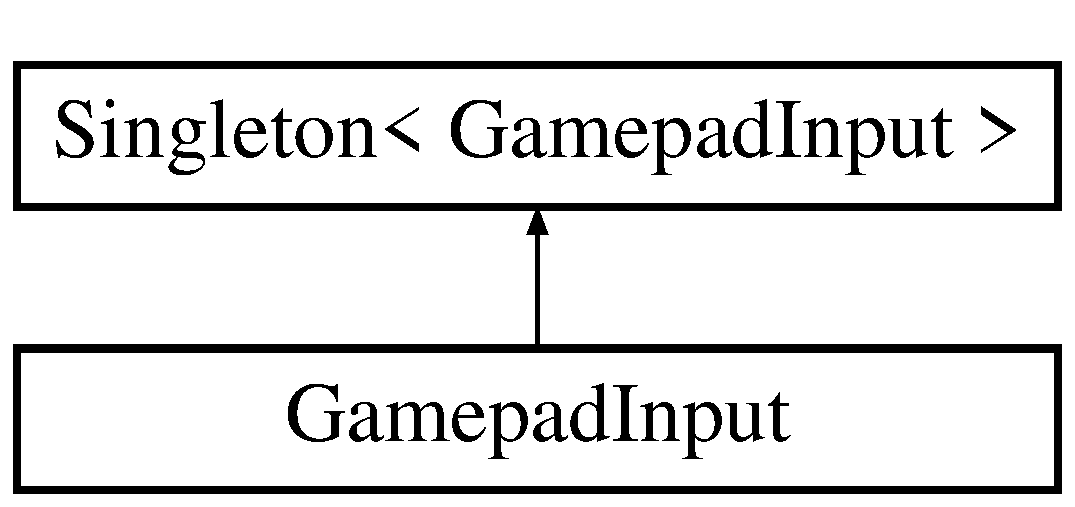
\includegraphics[height=2.000000cm]{class_gamepad_input}
\end{center}
\end{figure}
\subsection*{公開メンバ関数}
\begin{DoxyCompactItemize}
\item 
\mbox{\hyperlink{class_gamepad_input_acd9878326e438f379020827d63ebd6cf}{Gamepad\+Input}} ()
\begin{DoxyCompactList}\small\item\em コンストラクタで初期化 \end{DoxyCompactList}\item 
void \mbox{\hyperlink{class_gamepad_input_a3512c0cc4d57534c83db09c4b5377caa}{Update}} ()
\begin{DoxyCompactList}\small\item\em ゲームパッドインプットの更新 \end{DoxyCompactList}\item 
void \mbox{\hyperlink{class_gamepad_input_afd429d32d076130ff8a7df12037eaddd}{Vibration}} (size\+\_\+t index, float, float)
\begin{DoxyCompactList}\small\item\em コントローラーの振動 \end{DoxyCompactList}\item 
bool \mbox{\hyperlink{class_gamepad_input_a29a71d0503e038e55ffe282e2c768b05}{Get\+Button\+Down}} (size\+\_\+t index, \mbox{\hyperlink{gamepad__input_8h_a739845b0076428add52ca3cec492e705}{B\+U\+T\+T\+ON}} b) const
\begin{DoxyCompactList}\small\item\em --ゲッタ-- \end{DoxyCompactList}\item 
bool \mbox{\hyperlink{class_gamepad_input_a9a2f9042a5fa1c8e33fbd349f67747b3}{Get\+Button}} (size\+\_\+t index, \mbox{\hyperlink{gamepad__input_8h_a739845b0076428add52ca3cec492e705}{B\+U\+T\+T\+ON}} b) const
\begin{DoxyCompactList}\small\item\em ボタンを押しているかどうか \end{DoxyCompactList}\item 
bool \mbox{\hyperlink{class_gamepad_input_a5b76a114b8d3d03abbd2bcd91562109a}{Get\+Button\+Up}} (size\+\_\+t index, \mbox{\hyperlink{gamepad__input_8h_a739845b0076428add52ca3cec492e705}{B\+U\+T\+T\+ON}} b) const
\begin{DoxyCompactList}\small\item\em ボタンを離したかどうか \end{DoxyCompactList}\item 
float \mbox{\hyperlink{class_gamepad_input_a7e95e2a49cbd4729cf7156b9a703252a}{Get\+Trigger}} (size\+\_\+t index, const bool right) const
\begin{DoxyCompactList}\small\item\em トリガーの状態を返す \end{DoxyCompactList}\item 
float \mbox{\hyperlink{class_gamepad_input_a82333353a23ea0fa92bb87d6cf6592d8}{Get\+Stick}} (size\+\_\+t index, const bool right, const bool x) const
\begin{DoxyCompactList}\small\item\em スティックの状態を返す \end{DoxyCompactList}\end{DoxyCompactItemize}
\subsection*{その他の継承メンバ}


\subsection{詳解}
ゲームパッドのインプットクラス 

\subsection{構築子と解体子}
\mbox{\Hypertarget{class_gamepad_input_acd9878326e438f379020827d63ebd6cf}\label{class_gamepad_input_acd9878326e438f379020827d63ebd6cf}} 
\index{Gamepad\+Input@{Gamepad\+Input}!Gamepad\+Input@{Gamepad\+Input}}
\index{Gamepad\+Input@{Gamepad\+Input}!Gamepad\+Input@{Gamepad\+Input}}
\subsubsection{\texorpdfstring{Gamepad\+Input()}{GamepadInput()}}
{\footnotesize\ttfamily Gamepad\+Input\+::\+Gamepad\+Input (\begin{DoxyParamCaption}{ }\end{DoxyParamCaption})}



コンストラクタで初期化 



\subsection{関数詳解}
\mbox{\Hypertarget{class_gamepad_input_a9a2f9042a5fa1c8e33fbd349f67747b3}\label{class_gamepad_input_a9a2f9042a5fa1c8e33fbd349f67747b3}} 
\index{Gamepad\+Input@{Gamepad\+Input}!Get\+Button@{Get\+Button}}
\index{Get\+Button@{Get\+Button}!Gamepad\+Input@{Gamepad\+Input}}
\subsubsection{\texorpdfstring{Get\+Button()}{GetButton()}}
{\footnotesize\ttfamily bool Gamepad\+Input\+::\+Get\+Button (\begin{DoxyParamCaption}\item[{size\+\_\+t}]{index,  }\item[{\mbox{\hyperlink{gamepad__input_8h_a739845b0076428add52ca3cec492e705}{B\+U\+T\+T\+ON}}}]{b }\end{DoxyParamCaption}) const\hspace{0.3cm}{\ttfamily [inline]}}



ボタンを押しているかどうか 


\begin{DoxyParams}{引数}
{\em k} & 判定するボタン \\
\hline
\end{DoxyParams}
\mbox{\Hypertarget{class_gamepad_input_a29a71d0503e038e55ffe282e2c768b05}\label{class_gamepad_input_a29a71d0503e038e55ffe282e2c768b05}} 
\index{Gamepad\+Input@{Gamepad\+Input}!Get\+Button\+Down@{Get\+Button\+Down}}
\index{Get\+Button\+Down@{Get\+Button\+Down}!Gamepad\+Input@{Gamepad\+Input}}
\subsubsection{\texorpdfstring{Get\+Button\+Down()}{GetButtonDown()}}
{\footnotesize\ttfamily bool Gamepad\+Input\+::\+Get\+Button\+Down (\begin{DoxyParamCaption}\item[{size\+\_\+t}]{index,  }\item[{\mbox{\hyperlink{gamepad__input_8h_a739845b0076428add52ca3cec492e705}{B\+U\+T\+T\+ON}}}]{b }\end{DoxyParamCaption}) const\hspace{0.3cm}{\ttfamily [inline]}}



--ゲッタ-- 

ボタンを押したかどうか 
\begin{DoxyParams}{引数}
{\em k} & 判定するボタン \\
\hline
\end{DoxyParams}
\mbox{\Hypertarget{class_gamepad_input_a5b76a114b8d3d03abbd2bcd91562109a}\label{class_gamepad_input_a5b76a114b8d3d03abbd2bcd91562109a}} 
\index{Gamepad\+Input@{Gamepad\+Input}!Get\+Button\+Up@{Get\+Button\+Up}}
\index{Get\+Button\+Up@{Get\+Button\+Up}!Gamepad\+Input@{Gamepad\+Input}}
\subsubsection{\texorpdfstring{Get\+Button\+Up()}{GetButtonUp()}}
{\footnotesize\ttfamily bool Gamepad\+Input\+::\+Get\+Button\+Up (\begin{DoxyParamCaption}\item[{size\+\_\+t}]{index,  }\item[{\mbox{\hyperlink{gamepad__input_8h_a739845b0076428add52ca3cec492e705}{B\+U\+T\+T\+ON}}}]{b }\end{DoxyParamCaption}) const\hspace{0.3cm}{\ttfamily [inline]}}



ボタンを離したかどうか 


\begin{DoxyParams}{引数}
{\em k} & 判定するボタン \\
\hline
\end{DoxyParams}
\mbox{\Hypertarget{class_gamepad_input_a82333353a23ea0fa92bb87d6cf6592d8}\label{class_gamepad_input_a82333353a23ea0fa92bb87d6cf6592d8}} 
\index{Gamepad\+Input@{Gamepad\+Input}!Get\+Stick@{Get\+Stick}}
\index{Get\+Stick@{Get\+Stick}!Gamepad\+Input@{Gamepad\+Input}}
\subsubsection{\texorpdfstring{Get\+Stick()}{GetStick()}}
{\footnotesize\ttfamily float Gamepad\+Input\+::\+Get\+Stick (\begin{DoxyParamCaption}\item[{size\+\_\+t}]{index,  }\item[{const bool}]{right,  }\item[{const bool}]{x }\end{DoxyParamCaption}) const\hspace{0.3cm}{\ttfamily [inline]}}



スティックの状態を返す 


\begin{DoxyParams}{引数}
{\em right} & 判定するのが右かどうか \\
\hline
{\em right} & 判定するのがxかどうか \\
\hline
\end{DoxyParams}
\mbox{\Hypertarget{class_gamepad_input_a7e95e2a49cbd4729cf7156b9a703252a}\label{class_gamepad_input_a7e95e2a49cbd4729cf7156b9a703252a}} 
\index{Gamepad\+Input@{Gamepad\+Input}!Get\+Trigger@{Get\+Trigger}}
\index{Get\+Trigger@{Get\+Trigger}!Gamepad\+Input@{Gamepad\+Input}}
\subsubsection{\texorpdfstring{Get\+Trigger()}{GetTrigger()}}
{\footnotesize\ttfamily float Gamepad\+Input\+::\+Get\+Trigger (\begin{DoxyParamCaption}\item[{size\+\_\+t}]{index,  }\item[{const bool}]{right }\end{DoxyParamCaption}) const\hspace{0.3cm}{\ttfamily [inline]}}



トリガーの状態を返す 


\begin{DoxyParams}{引数}
{\em right} & 判定するのが右かどうか \\
\hline
\end{DoxyParams}
\mbox{\Hypertarget{class_gamepad_input_a3512c0cc4d57534c83db09c4b5377caa}\label{class_gamepad_input_a3512c0cc4d57534c83db09c4b5377caa}} 
\index{Gamepad\+Input@{Gamepad\+Input}!Update@{Update}}
\index{Update@{Update}!Gamepad\+Input@{Gamepad\+Input}}
\subsubsection{\texorpdfstring{Update()}{Update()}}
{\footnotesize\ttfamily void Gamepad\+Input\+::\+Update (\begin{DoxyParamCaption}{ }\end{DoxyParamCaption})}



ゲームパッドインプットの更新 

\mbox{\Hypertarget{class_gamepad_input_afd429d32d076130ff8a7df12037eaddd}\label{class_gamepad_input_afd429d32d076130ff8a7df12037eaddd}} 
\index{Gamepad\+Input@{Gamepad\+Input}!Vibration@{Vibration}}
\index{Vibration@{Vibration}!Gamepad\+Input@{Gamepad\+Input}}
\subsubsection{\texorpdfstring{Vibration()}{Vibration()}}
{\footnotesize\ttfamily void Gamepad\+Input\+::\+Vibration (\begin{DoxyParamCaption}\item[{size\+\_\+t}]{index,  }\item[{float}]{right,  }\item[{float}]{left }\end{DoxyParamCaption})}



コントローラーの振動 


\begin{DoxyParams}{引数}
{\em right} & 右のモーターの力 \\
\hline
{\em left} & 左のモーターの力 \\
\hline
\end{DoxyParams}


このクラス詳解は次のファイルから抽出されました\+:\begin{DoxyCompactItemize}
\item 
C\+:/\+Users/tokir/\+Documents/\+Git\+Hub/\+Weapon\+Merchant\+Adventure/src/src/input/gamepad/\mbox{\hyperlink{gamepad__input_8h}{gamepad\+\_\+input.\+h}}\item 
C\+:/\+Users/tokir/\+Documents/\+Git\+Hub/\+Weapon\+Merchant\+Adventure/src/src/input/gamepad/\mbox{\hyperlink{gamepad__input_8cpp}{gamepad\+\_\+input.\+cpp}}\end{DoxyCompactItemize}

\hypertarget{class_game_scene_base}{}\section{Game\+Scene\+Base クラス}
\label{class_game_scene_base}\index{Game\+Scene\+Base@{Game\+Scene\+Base}}


ゲームシーンのスーパークラス  




{\ttfamily \#include $<$game\+\_\+scene\+\_\+base.\+h$>$}

Game\+Scene\+Base の継承関係図\begin{figure}[H]
\begin{center}
\leavevmode
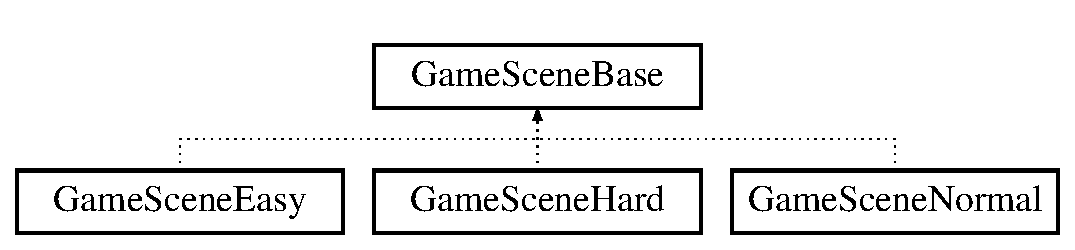
\includegraphics[height=2.000000cm]{class_game_scene_base}
\end{center}
\end{figure}
\subsection*{公開型}
\begin{DoxyCompactItemize}
\item 
enum \mbox{\hyperlink{class_game_scene_base_a9e25ffb879e1347e9605badaa53518f3}{G\+A\+ME}} \{ \newline
\mbox{\hyperlink{class_game_scene_base_a9e25ffb879e1347e9605badaa53518f3a186495f7da296bf880df3a22a492b378}{G\+A\+M\+E\+::\+M\+A\+IN}}, 
\mbox{\hyperlink{class_game_scene_base_a9e25ffb879e1347e9605badaa53518f3a0da044e5b37e6bcb3a8d01dc7362b276}{G\+A\+M\+E\+::\+T\+R\+A\+N\+S\+L\+A\+T\+I\+ON}}, 
\mbox{\hyperlink{class_game_scene_base_a9e25ffb879e1347e9605badaa53518f3af0523bf35faf77235783d0f3e43762d2}{G\+A\+M\+E\+::\+B\+O\+SS}}, 
\mbox{\hyperlink{class_game_scene_base_a9e25ffb879e1347e9605badaa53518f3a813461e0c58e7ad59a2fd83ca2237fec}{G\+A\+M\+E\+::\+C\+L\+E\+AR}}, 
\newline
\mbox{\hyperlink{class_game_scene_base_a9e25ffb879e1347e9605badaa53518f3ab50339a10e1de285ac99d4c3990b8693}{G\+A\+M\+E\+::\+N\+O\+NE}}
 \}
\end{DoxyCompactItemize}
\subsection*{公開メンバ関数}
\begin{DoxyCompactItemize}
\item 
void \mbox{\hyperlink{class_game_scene_base_ab37608f861866bd183801326214d0e92}{Game\+Init}} ()
\begin{DoxyCompactList}\small\item\em ゲームシーンの初期化 \end{DoxyCompactList}\item 
std\+::shared\+\_\+ptr$<$ \mbox{\hyperlink{class_scene}{Scene}} $>$ \mbox{\hyperlink{class_game_scene_base_ae9dab92c5cb057a884d12d21fe823fd9}{Game\+Update}} (std\+::shared\+\_\+ptr$<$ \mbox{\hyperlink{class_scene}{Scene}} $>$ \&)
\begin{DoxyCompactList}\small\item\em ゲームシーンの更新 \end{DoxyCompactList}\item 
void \mbox{\hyperlink{class_game_scene_base_acc15e7fb83c2403c2a5e65fa64ca8cb3}{Game\+Render}} ()
\begin{DoxyCompactList}\small\item\em ゲームシーンの描画 \end{DoxyCompactList}\item 
void \mbox{\hyperlink{class_game_scene_base_a8105804f1a8d6d59d4278d00142680a0}{Game\+Destroy}} ()
\begin{DoxyCompactList}\small\item\em ゲームシーンの破棄 \end{DoxyCompactList}\end{DoxyCompactItemize}
\subsection*{公開変数類}
\begin{DoxyCompactItemize}
\item 
bool \mbox{\hyperlink{class_game_scene_base_af752b345d7711c43c8deafd6618bb62f}{clear\+\_\+jump}} = false
\item 
\mbox{\hyperlink{class_game_scene_base_a9e25ffb879e1347e9605badaa53518f3}{G\+A\+ME}} \mbox{\hyperlink{class_game_scene_base_aad639837dc3d0735e69052c980ec9f18}{current\+\_\+game}} = \mbox{\hyperlink{class_game_scene_base_a9e25ffb879e1347e9605badaa53518f3a186495f7da296bf880df3a22a492b378}{G\+A\+M\+E\+::\+M\+A\+IN}}
\item 
std\+::list$<$ \mbox{\hyperlink{class_normal_enemy}{Normal\+Enemy}} $>$ \mbox{\hyperlink{class_game_scene_base_a5203f71e49d0a65de546dce23670b39e}{enemy}}
\item 
std\+::list$<$ \mbox{\hyperlink{class_fly_enemy}{Fly\+Enemy}} $>$ \mbox{\hyperlink{class_game_scene_base_ad34ad8c64d483b662352b9a806634bd9}{f\+\_\+enemy}}
\item 
std\+::unique\+\_\+ptr$<$ \mbox{\hyperlink{class_player}{Player}} $>$ \mbox{\hyperlink{class_game_scene_base_a86d056176f172dc0115d00878956a741}{player}}
\item 
std\+::unique\+\_\+ptr$<$ \mbox{\hyperlink{class_boss}{Boss}} $>$ \mbox{\hyperlink{class_game_scene_base_a8de41f067f4a7ed1e41f60836ea1b1e5}{boss}}
\item 
std\+::vector$<$ \mbox{\hyperlink{class_static_object}{Static\+Object}} $>$ \mbox{\hyperlink{class_game_scene_base_a0c60c7b970f081b2eee1ac14d74f6a7e}{back\+Ground}}
\item 
std\+::vector$<$ \mbox{\hyperlink{class_map_object}{Map\+Object}} $>$ \mbox{\hyperlink{class_game_scene_base_a27a6d9806fd1f23a651a545c94a24254}{field}}
\item 
std\+::list$<$ \mbox{\hyperlink{class_bullet_item}{Bullet\+Item}} $>$ \mbox{\hyperlink{class_game_scene_base_a32ec936c873df49cdf1400deb60c6b7f}{bullet\+\_\+item}}
\item 
float \mbox{\hyperlink{class_game_scene_base_a1eebaf57ec13050f35ae29074f10c668}{boss\+\_\+center\+\_\+x}}
\end{DoxyCompactItemize}


\subsection{詳解}
ゲームシーンのスーパークラス 

\subsection{列挙型メンバ詳解}
\mbox{\Hypertarget{class_game_scene_base_a9e25ffb879e1347e9605badaa53518f3}\label{class_game_scene_base_a9e25ffb879e1347e9605badaa53518f3}} 
\index{Game\+Scene\+Base@{Game\+Scene\+Base}!G\+A\+ME@{G\+A\+ME}}
\index{G\+A\+ME@{G\+A\+ME}!Game\+Scene\+Base@{Game\+Scene\+Base}}
\subsubsection{\texorpdfstring{G\+A\+ME}{GAME}}
{\footnotesize\ttfamily enum \mbox{\hyperlink{class_game_scene_base_a9e25ffb879e1347e9605badaa53518f3}{Game\+Scene\+Base\+::\+G\+A\+ME}}\hspace{0.3cm}{\ttfamily [strong]}}

\begin{DoxyEnumFields}{列挙値}
\raisebox{\heightof{T}}[0pt][0pt]{\index{M\+A\+IN@{M\+A\+IN}!Game\+Scene\+Base@{Game\+Scene\+Base}}\index{Game\+Scene\+Base@{Game\+Scene\+Base}!M\+A\+IN@{M\+A\+IN}}}\mbox{\Hypertarget{class_game_scene_base_a9e25ffb879e1347e9605badaa53518f3a186495f7da296bf880df3a22a492b378}\label{class_game_scene_base_a9e25ffb879e1347e9605badaa53518f3a186495f7da296bf880df3a22a492b378}} 
M\+A\+IN&\\
\hline

\raisebox{\heightof{T}}[0pt][0pt]{\index{T\+R\+A\+N\+S\+L\+A\+T\+I\+ON@{T\+R\+A\+N\+S\+L\+A\+T\+I\+ON}!Game\+Scene\+Base@{Game\+Scene\+Base}}\index{Game\+Scene\+Base@{Game\+Scene\+Base}!T\+R\+A\+N\+S\+L\+A\+T\+I\+ON@{T\+R\+A\+N\+S\+L\+A\+T\+I\+ON}}}\mbox{\Hypertarget{class_game_scene_base_a9e25ffb879e1347e9605badaa53518f3a0da044e5b37e6bcb3a8d01dc7362b276}\label{class_game_scene_base_a9e25ffb879e1347e9605badaa53518f3a0da044e5b37e6bcb3a8d01dc7362b276}} 
T\+R\+A\+N\+S\+L\+A\+T\+I\+ON&\\
\hline

\raisebox{\heightof{T}}[0pt][0pt]{\index{B\+O\+SS@{B\+O\+SS}!Game\+Scene\+Base@{Game\+Scene\+Base}}\index{Game\+Scene\+Base@{Game\+Scene\+Base}!B\+O\+SS@{B\+O\+SS}}}\mbox{\Hypertarget{class_game_scene_base_a9e25ffb879e1347e9605badaa53518f3af0523bf35faf77235783d0f3e43762d2}\label{class_game_scene_base_a9e25ffb879e1347e9605badaa53518f3af0523bf35faf77235783d0f3e43762d2}} 
B\+O\+SS&\\
\hline

\raisebox{\heightof{T}}[0pt][0pt]{\index{C\+L\+E\+AR@{C\+L\+E\+AR}!Game\+Scene\+Base@{Game\+Scene\+Base}}\index{Game\+Scene\+Base@{Game\+Scene\+Base}!C\+L\+E\+AR@{C\+L\+E\+AR}}}\mbox{\Hypertarget{class_game_scene_base_a9e25ffb879e1347e9605badaa53518f3a813461e0c58e7ad59a2fd83ca2237fec}\label{class_game_scene_base_a9e25ffb879e1347e9605badaa53518f3a813461e0c58e7ad59a2fd83ca2237fec}} 
C\+L\+E\+AR&\\
\hline

\raisebox{\heightof{T}}[0pt][0pt]{\index{N\+O\+NE@{N\+O\+NE}!Game\+Scene\+Base@{Game\+Scene\+Base}}\index{Game\+Scene\+Base@{Game\+Scene\+Base}!N\+O\+NE@{N\+O\+NE}}}\mbox{\Hypertarget{class_game_scene_base_a9e25ffb879e1347e9605badaa53518f3ab50339a10e1de285ac99d4c3990b8693}\label{class_game_scene_base_a9e25ffb879e1347e9605badaa53518f3ab50339a10e1de285ac99d4c3990b8693}} 
N\+O\+NE&\\
\hline

\end{DoxyEnumFields}


\subsection{関数詳解}
\mbox{\Hypertarget{class_game_scene_base_a8105804f1a8d6d59d4278d00142680a0}\label{class_game_scene_base_a8105804f1a8d6d59d4278d00142680a0}} 
\index{Game\+Scene\+Base@{Game\+Scene\+Base}!Game\+Destroy@{Game\+Destroy}}
\index{Game\+Destroy@{Game\+Destroy}!Game\+Scene\+Base@{Game\+Scene\+Base}}
\subsubsection{\texorpdfstring{Game\+Destroy()}{GameDestroy()}}
{\footnotesize\ttfamily void Game\+Scene\+Base\+::\+Game\+Destroy (\begin{DoxyParamCaption}{ }\end{DoxyParamCaption})}



ゲームシーンの破棄 

\mbox{\Hypertarget{class_game_scene_base_ab37608f861866bd183801326214d0e92}\label{class_game_scene_base_ab37608f861866bd183801326214d0e92}} 
\index{Game\+Scene\+Base@{Game\+Scene\+Base}!Game\+Init@{Game\+Init}}
\index{Game\+Init@{Game\+Init}!Game\+Scene\+Base@{Game\+Scene\+Base}}
\subsubsection{\texorpdfstring{Game\+Init()}{GameInit()}}
{\footnotesize\ttfamily void Game\+Scene\+Base\+::\+Game\+Init (\begin{DoxyParamCaption}{ }\end{DoxyParamCaption})}



ゲームシーンの初期化 

\mbox{\Hypertarget{class_game_scene_base_acc15e7fb83c2403c2a5e65fa64ca8cb3}\label{class_game_scene_base_acc15e7fb83c2403c2a5e65fa64ca8cb3}} 
\index{Game\+Scene\+Base@{Game\+Scene\+Base}!Game\+Render@{Game\+Render}}
\index{Game\+Render@{Game\+Render}!Game\+Scene\+Base@{Game\+Scene\+Base}}
\subsubsection{\texorpdfstring{Game\+Render()}{GameRender()}}
{\footnotesize\ttfamily void Game\+Scene\+Base\+::\+Game\+Render (\begin{DoxyParamCaption}{ }\end{DoxyParamCaption})}



ゲームシーンの描画 

\mbox{\Hypertarget{class_game_scene_base_ae9dab92c5cb057a884d12d21fe823fd9}\label{class_game_scene_base_ae9dab92c5cb057a884d12d21fe823fd9}} 
\index{Game\+Scene\+Base@{Game\+Scene\+Base}!Game\+Update@{Game\+Update}}
\index{Game\+Update@{Game\+Update}!Game\+Scene\+Base@{Game\+Scene\+Base}}
\subsubsection{\texorpdfstring{Game\+Update()}{GameUpdate()}}
{\footnotesize\ttfamily std\+::shared\+\_\+ptr$<$ \mbox{\hyperlink{class_scene}{Scene}} $>$ Game\+Scene\+Base\+::\+Game\+Update (\begin{DoxyParamCaption}\item[{std\+::shared\+\_\+ptr$<$ \mbox{\hyperlink{class_scene}{Scene}} $>$ \&}]{scene }\end{DoxyParamCaption})}



ゲームシーンの更新 

\begin{DoxyReturn}{戻り値}
std\+::shared\+\_\+ptr$<$\+Scene$>$ シーンが変わるなら次のシーンのstd\+::shared\+\_\+ptr$<$\+Scene$>$を返す 
\end{DoxyReturn}


\subsection{メンバ詳解}
\mbox{\Hypertarget{class_game_scene_base_a0c60c7b970f081b2eee1ac14d74f6a7e}\label{class_game_scene_base_a0c60c7b970f081b2eee1ac14d74f6a7e}} 
\index{Game\+Scene\+Base@{Game\+Scene\+Base}!back\+Ground@{back\+Ground}}
\index{back\+Ground@{back\+Ground}!Game\+Scene\+Base@{Game\+Scene\+Base}}
\subsubsection{\texorpdfstring{back\+Ground}{backGround}}
{\footnotesize\ttfamily std\+::vector$<$\mbox{\hyperlink{class_static_object}{Static\+Object}}$>$ Game\+Scene\+Base\+::back\+Ground}

\mbox{\Hypertarget{class_game_scene_base_a8de41f067f4a7ed1e41f60836ea1b1e5}\label{class_game_scene_base_a8de41f067f4a7ed1e41f60836ea1b1e5}} 
\index{Game\+Scene\+Base@{Game\+Scene\+Base}!boss@{boss}}
\index{boss@{boss}!Game\+Scene\+Base@{Game\+Scene\+Base}}
\subsubsection{\texorpdfstring{boss}{boss}}
{\footnotesize\ttfamily std\+::unique\+\_\+ptr$<$\mbox{\hyperlink{class_boss}{Boss}}$>$ Game\+Scene\+Base\+::boss}

\mbox{\Hypertarget{class_game_scene_base_a1eebaf57ec13050f35ae29074f10c668}\label{class_game_scene_base_a1eebaf57ec13050f35ae29074f10c668}} 
\index{Game\+Scene\+Base@{Game\+Scene\+Base}!boss\+\_\+center\+\_\+x@{boss\+\_\+center\+\_\+x}}
\index{boss\+\_\+center\+\_\+x@{boss\+\_\+center\+\_\+x}!Game\+Scene\+Base@{Game\+Scene\+Base}}
\subsubsection{\texorpdfstring{boss\+\_\+center\+\_\+x}{boss\_center\_x}}
{\footnotesize\ttfamily float Game\+Scene\+Base\+::boss\+\_\+center\+\_\+x}

\mbox{\Hypertarget{class_game_scene_base_a32ec936c873df49cdf1400deb60c6b7f}\label{class_game_scene_base_a32ec936c873df49cdf1400deb60c6b7f}} 
\index{Game\+Scene\+Base@{Game\+Scene\+Base}!bullet\+\_\+item@{bullet\+\_\+item}}
\index{bullet\+\_\+item@{bullet\+\_\+item}!Game\+Scene\+Base@{Game\+Scene\+Base}}
\subsubsection{\texorpdfstring{bullet\+\_\+item}{bullet\_item}}
{\footnotesize\ttfamily std\+::list$<$\mbox{\hyperlink{class_bullet_item}{Bullet\+Item}}$>$ Game\+Scene\+Base\+::bullet\+\_\+item}

\mbox{\Hypertarget{class_game_scene_base_af752b345d7711c43c8deafd6618bb62f}\label{class_game_scene_base_af752b345d7711c43c8deafd6618bb62f}} 
\index{Game\+Scene\+Base@{Game\+Scene\+Base}!clear\+\_\+jump@{clear\+\_\+jump}}
\index{clear\+\_\+jump@{clear\+\_\+jump}!Game\+Scene\+Base@{Game\+Scene\+Base}}
\subsubsection{\texorpdfstring{clear\+\_\+jump}{clear\_jump}}
{\footnotesize\ttfamily bool Game\+Scene\+Base\+::clear\+\_\+jump = false}

\mbox{\Hypertarget{class_game_scene_base_aad639837dc3d0735e69052c980ec9f18}\label{class_game_scene_base_aad639837dc3d0735e69052c980ec9f18}} 
\index{Game\+Scene\+Base@{Game\+Scene\+Base}!current\+\_\+game@{current\+\_\+game}}
\index{current\+\_\+game@{current\+\_\+game}!Game\+Scene\+Base@{Game\+Scene\+Base}}
\subsubsection{\texorpdfstring{current\+\_\+game}{current\_game}}
{\footnotesize\ttfamily \mbox{\hyperlink{class_game_scene_base_a9e25ffb879e1347e9605badaa53518f3}{G\+A\+ME}} Game\+Scene\+Base\+::current\+\_\+game = \mbox{\hyperlink{class_game_scene_base_a9e25ffb879e1347e9605badaa53518f3a186495f7da296bf880df3a22a492b378}{G\+A\+M\+E\+::\+M\+A\+IN}}}

\mbox{\Hypertarget{class_game_scene_base_a5203f71e49d0a65de546dce23670b39e}\label{class_game_scene_base_a5203f71e49d0a65de546dce23670b39e}} 
\index{Game\+Scene\+Base@{Game\+Scene\+Base}!enemy@{enemy}}
\index{enemy@{enemy}!Game\+Scene\+Base@{Game\+Scene\+Base}}
\subsubsection{\texorpdfstring{enemy}{enemy}}
{\footnotesize\ttfamily std\+::list$<$\mbox{\hyperlink{class_normal_enemy}{Normal\+Enemy}}$>$ Game\+Scene\+Base\+::enemy}

\mbox{\Hypertarget{class_game_scene_base_ad34ad8c64d483b662352b9a806634bd9}\label{class_game_scene_base_ad34ad8c64d483b662352b9a806634bd9}} 
\index{Game\+Scene\+Base@{Game\+Scene\+Base}!f\+\_\+enemy@{f\+\_\+enemy}}
\index{f\+\_\+enemy@{f\+\_\+enemy}!Game\+Scene\+Base@{Game\+Scene\+Base}}
\subsubsection{\texorpdfstring{f\+\_\+enemy}{f\_enemy}}
{\footnotesize\ttfamily std\+::list$<$\mbox{\hyperlink{class_fly_enemy}{Fly\+Enemy}}$>$ Game\+Scene\+Base\+::f\+\_\+enemy}

\mbox{\Hypertarget{class_game_scene_base_a27a6d9806fd1f23a651a545c94a24254}\label{class_game_scene_base_a27a6d9806fd1f23a651a545c94a24254}} 
\index{Game\+Scene\+Base@{Game\+Scene\+Base}!field@{field}}
\index{field@{field}!Game\+Scene\+Base@{Game\+Scene\+Base}}
\subsubsection{\texorpdfstring{field}{field}}
{\footnotesize\ttfamily std\+::vector$<$\mbox{\hyperlink{class_map_object}{Map\+Object}}$>$ Game\+Scene\+Base\+::field}

\mbox{\Hypertarget{class_game_scene_base_a86d056176f172dc0115d00878956a741}\label{class_game_scene_base_a86d056176f172dc0115d00878956a741}} 
\index{Game\+Scene\+Base@{Game\+Scene\+Base}!player@{player}}
\index{player@{player}!Game\+Scene\+Base@{Game\+Scene\+Base}}
\subsubsection{\texorpdfstring{player}{player}}
{\footnotesize\ttfamily std\+::unique\+\_\+ptr$<$\mbox{\hyperlink{class_player}{Player}}$>$ Game\+Scene\+Base\+::player}



このクラス詳解は次のファイルから抽出されました\+:\begin{DoxyCompactItemize}
\item 
C\+:/\+Users/tokir/\+Documents/\+Git\+Hub/\+Weapon\+Merchant\+Adventure/src/src/scene/main/game/base/\mbox{\hyperlink{game__scene__base_8h}{game\+\_\+scene\+\_\+base.\+h}}\item 
C\+:/\+Users/tokir/\+Documents/\+Git\+Hub/\+Weapon\+Merchant\+Adventure/src/src/scene/main/game/base/\mbox{\hyperlink{game__scene__base_8cpp}{game\+\_\+scene\+\_\+base.\+cpp}}\end{DoxyCompactItemize}

\hypertarget{class_game_scene_easy}{}\section{Game\+Scene\+Easy クラス}
\label{class_game_scene_easy}\index{Game\+Scene\+Easy@{Game\+Scene\+Easy}}


ゲームシーン(easy)クラス  




{\ttfamily \#include $<$game\+\_\+scene\+\_\+easy.\+h$>$}

Game\+Scene\+Easy の継承関係図\begin{figure}[H]
\begin{center}
\leavevmode
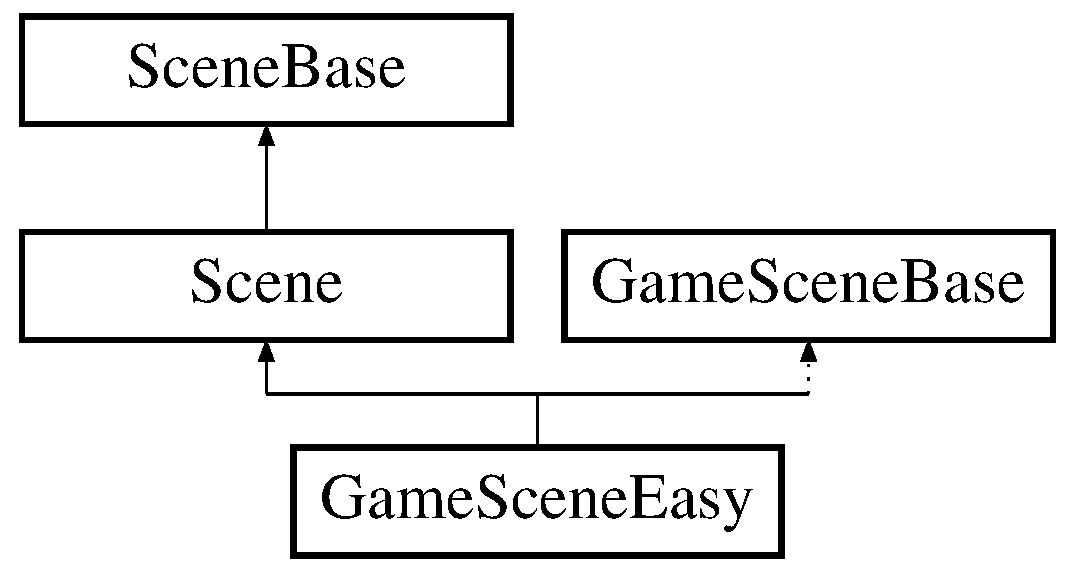
\includegraphics[height=3.000000cm]{class_game_scene_easy}
\end{center}
\end{figure}
\subsection*{公開メンバ関数}
\begin{DoxyCompactItemize}
\item 
void \mbox{\hyperlink{class_game_scene_easy_a837e9b0c8227dca2d14f975a8f007ed1}{Init}} () final
\begin{DoxyCompactList}\small\item\em ゲームシーン(easy)の初期化 \end{DoxyCompactList}\item 
std\+::shared\+\_\+ptr$<$ \mbox{\hyperlink{class_scene}{Scene}} $>$ \mbox{\hyperlink{class_game_scene_easy_ac2bccbf61722010fd6f317693ee7b8b1}{Update}} (std\+::shared\+\_\+ptr$<$ \mbox{\hyperlink{class_scene}{Scene}} $>$ \&) final
\begin{DoxyCompactList}\small\item\em ゲームシーン(easy)の更新 \end{DoxyCompactList}\item 
void \mbox{\hyperlink{class_game_scene_easy_ad2cbe509b1f81f0e3b4d1656466dabd3}{Render}} () final
\begin{DoxyCompactList}\small\item\em ゲームシーン(easy)の描画 \end{DoxyCompactList}\item 
void \mbox{\hyperlink{class_game_scene_easy_aadbe3ec3a28639abca94c7868a0a97df}{Destroy}} () final
\begin{DoxyCompactList}\small\item\em ゲームシーン(easy)の破棄 \end{DoxyCompactList}\end{DoxyCompactItemize}


\subsection{詳解}
ゲームシーン(easy)クラス 

\subsection{関数詳解}
\mbox{\Hypertarget{class_game_scene_easy_aadbe3ec3a28639abca94c7868a0a97df}\label{class_game_scene_easy_aadbe3ec3a28639abca94c7868a0a97df}} 
\index{Game\+Scene\+Easy@{Game\+Scene\+Easy}!Destroy@{Destroy}}
\index{Destroy@{Destroy}!Game\+Scene\+Easy@{Game\+Scene\+Easy}}
\subsubsection{\texorpdfstring{Destroy()}{Destroy()}}
{\footnotesize\ttfamily void Game\+Scene\+Easy\+::\+Destroy (\begin{DoxyParamCaption}{ }\end{DoxyParamCaption})\hspace{0.3cm}{\ttfamily [final]}, {\ttfamily [virtual]}}



ゲームシーン(easy)の破棄 



\mbox{\hyperlink{class_scene_base_a7c5b54020bc519b4dadfe9770d6b27f7}{Scene\+Base}}を実装しています。

\mbox{\Hypertarget{class_game_scene_easy_a837e9b0c8227dca2d14f975a8f007ed1}\label{class_game_scene_easy_a837e9b0c8227dca2d14f975a8f007ed1}} 
\index{Game\+Scene\+Easy@{Game\+Scene\+Easy}!Init@{Init}}
\index{Init@{Init}!Game\+Scene\+Easy@{Game\+Scene\+Easy}}
\subsubsection{\texorpdfstring{Init()}{Init()}}
{\footnotesize\ttfamily void Game\+Scene\+Easy\+::\+Init (\begin{DoxyParamCaption}{ }\end{DoxyParamCaption})\hspace{0.3cm}{\ttfamily [final]}, {\ttfamily [virtual]}}



ゲームシーン(easy)の初期化 



\mbox{\hyperlink{class_scene_base_a24d7db43c819924dc8b07b436f6d3148}{Scene\+Base}}を実装しています。

\mbox{\Hypertarget{class_game_scene_easy_ad2cbe509b1f81f0e3b4d1656466dabd3}\label{class_game_scene_easy_ad2cbe509b1f81f0e3b4d1656466dabd3}} 
\index{Game\+Scene\+Easy@{Game\+Scene\+Easy}!Render@{Render}}
\index{Render@{Render}!Game\+Scene\+Easy@{Game\+Scene\+Easy}}
\subsubsection{\texorpdfstring{Render()}{Render()}}
{\footnotesize\ttfamily void Game\+Scene\+Easy\+::\+Render (\begin{DoxyParamCaption}{ }\end{DoxyParamCaption})\hspace{0.3cm}{\ttfamily [final]}, {\ttfamily [virtual]}}



ゲームシーン(easy)の描画 



\mbox{\hyperlink{class_scene_base_ad981674ce731ea267f398e889bbb9dc3}{Scene\+Base}}を実装しています。

\mbox{\Hypertarget{class_game_scene_easy_ac2bccbf61722010fd6f317693ee7b8b1}\label{class_game_scene_easy_ac2bccbf61722010fd6f317693ee7b8b1}} 
\index{Game\+Scene\+Easy@{Game\+Scene\+Easy}!Update@{Update}}
\index{Update@{Update}!Game\+Scene\+Easy@{Game\+Scene\+Easy}}
\subsubsection{\texorpdfstring{Update()}{Update()}}
{\footnotesize\ttfamily std\+::shared\+\_\+ptr$<$ \mbox{\hyperlink{class_scene}{Scene}} $>$ Game\+Scene\+Easy\+::\+Update (\begin{DoxyParamCaption}\item[{std\+::shared\+\_\+ptr$<$ \mbox{\hyperlink{class_scene}{Scene}} $>$ \&}]{scene }\end{DoxyParamCaption})\hspace{0.3cm}{\ttfamily [final]}, {\ttfamily [virtual]}}



ゲームシーン(easy)の更新 

\begin{DoxyReturn}{戻り値}
std\+::shared\+\_\+ptr$<$\+Scene$>$ シーンが変わるなら次のシーンのstd\+::shared\+\_\+ptr$<$\+Scene$>$を返す 
\end{DoxyReturn}


\mbox{\hyperlink{class_scene_ab71ee5f19764b90c87b4574aa1cb1d25}{Scene}}を実装しています。



このクラス詳解は次のファイルから抽出されました\+:\begin{DoxyCompactItemize}
\item 
C\+:/\+Users/tokir/\+Documents/\+Git\+Hub/\+Weapon\+Merchant\+Adventure/src/src/scene/main/game/easy/\mbox{\hyperlink{game__scene__easy_8h}{game\+\_\+scene\+\_\+easy.\+h}}\item 
C\+:/\+Users/tokir/\+Documents/\+Git\+Hub/\+Weapon\+Merchant\+Adventure/src/src/scene/main/game/easy/\mbox{\hyperlink{game__scene__easy_8cpp}{game\+\_\+scene\+\_\+easy.\+cpp}}\end{DoxyCompactItemize}

\hypertarget{class_game_scene_hard}{}\section{Game\+Scene\+Hard クラス}
\label{class_game_scene_hard}\index{Game\+Scene\+Hard@{Game\+Scene\+Hard}}


ゲームシーン(hard)クラス  




{\ttfamily \#include $<$game\+\_\+scene\+\_\+hard.\+h$>$}

Game\+Scene\+Hard の継承関係図\begin{figure}[H]
\begin{center}
\leavevmode
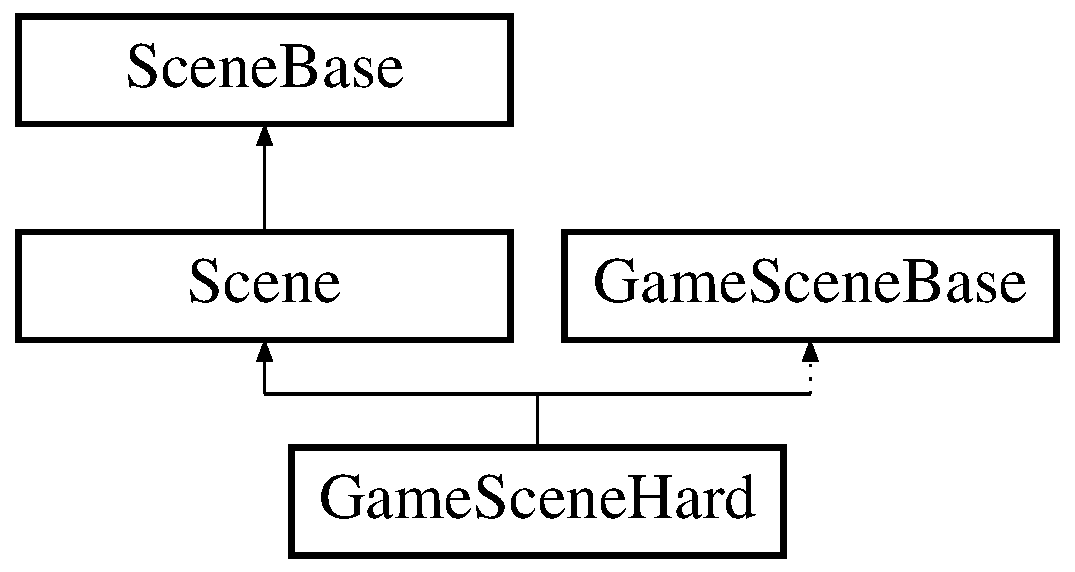
\includegraphics[height=3.000000cm]{class_game_scene_hard}
\end{center}
\end{figure}
\subsection*{公開メンバ関数}
\begin{DoxyCompactItemize}
\item 
void \mbox{\hyperlink{class_game_scene_hard_affc2e6a09c13a625730eeb0e742cb22a}{Init}} () final
\begin{DoxyCompactList}\small\item\em ゲームシーン(hard)の初期化 \end{DoxyCompactList}\item 
std\+::shared\+\_\+ptr$<$ \mbox{\hyperlink{class_scene}{Scene}} $>$ \mbox{\hyperlink{class_game_scene_hard_ac132a0e281a7d4e6b71deb6e5bcfdb9d}{Update}} (std\+::shared\+\_\+ptr$<$ \mbox{\hyperlink{class_scene}{Scene}} $>$ \&) final
\begin{DoxyCompactList}\small\item\em ゲームシーン(hard)の更新 \end{DoxyCompactList}\item 
void \mbox{\hyperlink{class_game_scene_hard_ab4d10e5fc6e39746f80ef967d6a02eae}{Render}} () final
\begin{DoxyCompactList}\small\item\em ゲームシーン(hard)の描画 \end{DoxyCompactList}\item 
void \mbox{\hyperlink{class_game_scene_hard_a7a2ddc79c737ede4d1125d352c5756c1}{Destroy}} () final
\begin{DoxyCompactList}\small\item\em ゲームシーン(hard)の破棄 \end{DoxyCompactList}\end{DoxyCompactItemize}


\subsection{詳解}
ゲームシーン(hard)クラス 

\subsection{関数詳解}
\mbox{\Hypertarget{class_game_scene_hard_a7a2ddc79c737ede4d1125d352c5756c1}\label{class_game_scene_hard_a7a2ddc79c737ede4d1125d352c5756c1}} 
\index{Game\+Scene\+Hard@{Game\+Scene\+Hard}!Destroy@{Destroy}}
\index{Destroy@{Destroy}!Game\+Scene\+Hard@{Game\+Scene\+Hard}}
\subsubsection{\texorpdfstring{Destroy()}{Destroy()}}
{\footnotesize\ttfamily void Game\+Scene\+Hard\+::\+Destroy (\begin{DoxyParamCaption}{ }\end{DoxyParamCaption})\hspace{0.3cm}{\ttfamily [final]}, {\ttfamily [virtual]}}



ゲームシーン(hard)の破棄 



\mbox{\hyperlink{class_scene_base_a7c5b54020bc519b4dadfe9770d6b27f7}{Scene\+Base}}を実装しています。

\mbox{\Hypertarget{class_game_scene_hard_affc2e6a09c13a625730eeb0e742cb22a}\label{class_game_scene_hard_affc2e6a09c13a625730eeb0e742cb22a}} 
\index{Game\+Scene\+Hard@{Game\+Scene\+Hard}!Init@{Init}}
\index{Init@{Init}!Game\+Scene\+Hard@{Game\+Scene\+Hard}}
\subsubsection{\texorpdfstring{Init()}{Init()}}
{\footnotesize\ttfamily void Game\+Scene\+Hard\+::\+Init (\begin{DoxyParamCaption}{ }\end{DoxyParamCaption})\hspace{0.3cm}{\ttfamily [final]}, {\ttfamily [virtual]}}



ゲームシーン(hard)の初期化 



\mbox{\hyperlink{class_scene_base_a24d7db43c819924dc8b07b436f6d3148}{Scene\+Base}}を実装しています。

\mbox{\Hypertarget{class_game_scene_hard_ab4d10e5fc6e39746f80ef967d6a02eae}\label{class_game_scene_hard_ab4d10e5fc6e39746f80ef967d6a02eae}} 
\index{Game\+Scene\+Hard@{Game\+Scene\+Hard}!Render@{Render}}
\index{Render@{Render}!Game\+Scene\+Hard@{Game\+Scene\+Hard}}
\subsubsection{\texorpdfstring{Render()}{Render()}}
{\footnotesize\ttfamily void Game\+Scene\+Hard\+::\+Render (\begin{DoxyParamCaption}{ }\end{DoxyParamCaption})\hspace{0.3cm}{\ttfamily [final]}, {\ttfamily [virtual]}}



ゲームシーン(hard)の描画 



\mbox{\hyperlink{class_scene_base_ad981674ce731ea267f398e889bbb9dc3}{Scene\+Base}}を実装しています。

\mbox{\Hypertarget{class_game_scene_hard_ac132a0e281a7d4e6b71deb6e5bcfdb9d}\label{class_game_scene_hard_ac132a0e281a7d4e6b71deb6e5bcfdb9d}} 
\index{Game\+Scene\+Hard@{Game\+Scene\+Hard}!Update@{Update}}
\index{Update@{Update}!Game\+Scene\+Hard@{Game\+Scene\+Hard}}
\subsubsection{\texorpdfstring{Update()}{Update()}}
{\footnotesize\ttfamily std\+::shared\+\_\+ptr$<$ \mbox{\hyperlink{class_scene}{Scene}} $>$ Game\+Scene\+Hard\+::\+Update (\begin{DoxyParamCaption}\item[{std\+::shared\+\_\+ptr$<$ \mbox{\hyperlink{class_scene}{Scene}} $>$ \&}]{scene }\end{DoxyParamCaption})\hspace{0.3cm}{\ttfamily [final]}, {\ttfamily [virtual]}}



ゲームシーン(hard)の更新 

\begin{DoxyReturn}{戻り値}
std\+::shared\+\_\+ptr$<$\+Scene$>$ シーンが変わるなら次のシーンのstd\+::shared\+\_\+ptr$<$\+Scene$>$を返す 
\end{DoxyReturn}


\mbox{\hyperlink{class_scene_ab71ee5f19764b90c87b4574aa1cb1d25}{Scene}}を実装しています。



このクラス詳解は次のファイルから抽出されました\+:\begin{DoxyCompactItemize}
\item 
C\+:/\+Users/tokir/\+Documents/\+Git\+Hub/\+Weapon\+Merchant\+Adventure/src/src/scene/main/game/hard/\mbox{\hyperlink{game__scene__hard_8h}{game\+\_\+scene\+\_\+hard.\+h}}\item 
C\+:/\+Users/tokir/\+Documents/\+Git\+Hub/\+Weapon\+Merchant\+Adventure/src/src/scene/main/game/hard/\mbox{\hyperlink{game__scene__hard_8cpp}{game\+\_\+scene\+\_\+hard.\+cpp}}\end{DoxyCompactItemize}

\hypertarget{class_game_scene_normal}{}\section{Game\+Scene\+Normal クラス}
\label{class_game_scene_normal}\index{Game\+Scene\+Normal@{Game\+Scene\+Normal}}


ゲームシーン(normal)クラス  




{\ttfamily \#include $<$game\+\_\+scene\+\_\+normal.\+h$>$}

Game\+Scene\+Normal の継承関係図\begin{figure}[H]
\begin{center}
\leavevmode
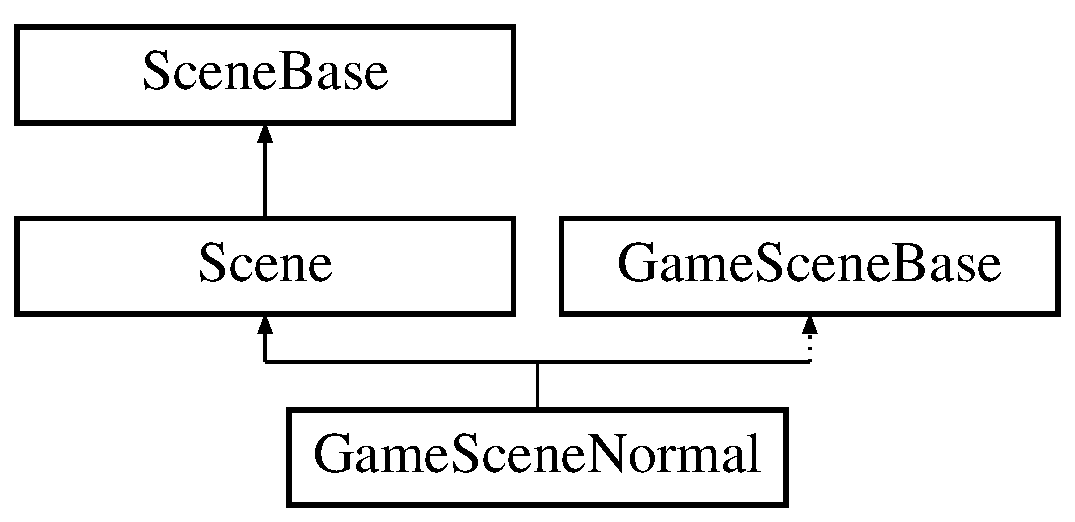
\includegraphics[height=3.000000cm]{class_game_scene_normal}
\end{center}
\end{figure}
\subsection*{公開メンバ関数}
\begin{DoxyCompactItemize}
\item 
void \mbox{\hyperlink{class_game_scene_normal_ac3f3e52cf1c24802035f38fccb221fd3}{Init}} () final
\begin{DoxyCompactList}\small\item\em ゲームシーン(normal)の初期化 \end{DoxyCompactList}\item 
std\+::shared\+\_\+ptr$<$ \mbox{\hyperlink{class_scene}{Scene}} $>$ \mbox{\hyperlink{class_game_scene_normal_a3e45ac3882f1d0dd5c77ab4f0a1ccb33}{Update}} (std\+::shared\+\_\+ptr$<$ \mbox{\hyperlink{class_scene}{Scene}} $>$ \&) final
\begin{DoxyCompactList}\small\item\em ゲームシーン(normal)の更新 \end{DoxyCompactList}\item 
void \mbox{\hyperlink{class_game_scene_normal_a1f0ef0b5b194f9f9e7bf857cca7acc39}{Render}} () final
\begin{DoxyCompactList}\small\item\em ゲームシーン(normal)の描画 \end{DoxyCompactList}\item 
void \mbox{\hyperlink{class_game_scene_normal_a1c06daa1715624eabd199472a37d97cd}{Destroy}} () final
\begin{DoxyCompactList}\small\item\em ゲームシーン(normal)の破棄 \end{DoxyCompactList}\end{DoxyCompactItemize}


\subsection{詳解}
ゲームシーン(normal)クラス 

\subsection{関数詳解}
\mbox{\Hypertarget{class_game_scene_normal_a1c06daa1715624eabd199472a37d97cd}\label{class_game_scene_normal_a1c06daa1715624eabd199472a37d97cd}} 
\index{Game\+Scene\+Normal@{Game\+Scene\+Normal}!Destroy@{Destroy}}
\index{Destroy@{Destroy}!Game\+Scene\+Normal@{Game\+Scene\+Normal}}
\subsubsection{\texorpdfstring{Destroy()}{Destroy()}}
{\footnotesize\ttfamily void Game\+Scene\+Normal\+::\+Destroy (\begin{DoxyParamCaption}{ }\end{DoxyParamCaption})\hspace{0.3cm}{\ttfamily [final]}, {\ttfamily [virtual]}}



ゲームシーン(normal)の破棄 



\mbox{\hyperlink{class_scene_base_a7c5b54020bc519b4dadfe9770d6b27f7}{Scene\+Base}}を実装しています。

\mbox{\Hypertarget{class_game_scene_normal_ac3f3e52cf1c24802035f38fccb221fd3}\label{class_game_scene_normal_ac3f3e52cf1c24802035f38fccb221fd3}} 
\index{Game\+Scene\+Normal@{Game\+Scene\+Normal}!Init@{Init}}
\index{Init@{Init}!Game\+Scene\+Normal@{Game\+Scene\+Normal}}
\subsubsection{\texorpdfstring{Init()}{Init()}}
{\footnotesize\ttfamily void Game\+Scene\+Normal\+::\+Init (\begin{DoxyParamCaption}{ }\end{DoxyParamCaption})\hspace{0.3cm}{\ttfamily [final]}, {\ttfamily [virtual]}}



ゲームシーン(normal)の初期化 



\mbox{\hyperlink{class_scene_base_a24d7db43c819924dc8b07b436f6d3148}{Scene\+Base}}を実装しています。

\mbox{\Hypertarget{class_game_scene_normal_a1f0ef0b5b194f9f9e7bf857cca7acc39}\label{class_game_scene_normal_a1f0ef0b5b194f9f9e7bf857cca7acc39}} 
\index{Game\+Scene\+Normal@{Game\+Scene\+Normal}!Render@{Render}}
\index{Render@{Render}!Game\+Scene\+Normal@{Game\+Scene\+Normal}}
\subsubsection{\texorpdfstring{Render()}{Render()}}
{\footnotesize\ttfamily void Game\+Scene\+Normal\+::\+Render (\begin{DoxyParamCaption}{ }\end{DoxyParamCaption})\hspace{0.3cm}{\ttfamily [final]}, {\ttfamily [virtual]}}



ゲームシーン(normal)の描画 



\mbox{\hyperlink{class_scene_base_ad981674ce731ea267f398e889bbb9dc3}{Scene\+Base}}を実装しています。

\mbox{\Hypertarget{class_game_scene_normal_a3e45ac3882f1d0dd5c77ab4f0a1ccb33}\label{class_game_scene_normal_a3e45ac3882f1d0dd5c77ab4f0a1ccb33}} 
\index{Game\+Scene\+Normal@{Game\+Scene\+Normal}!Update@{Update}}
\index{Update@{Update}!Game\+Scene\+Normal@{Game\+Scene\+Normal}}
\subsubsection{\texorpdfstring{Update()}{Update()}}
{\footnotesize\ttfamily std\+::shared\+\_\+ptr$<$ \mbox{\hyperlink{class_scene}{Scene}} $>$ Game\+Scene\+Normal\+::\+Update (\begin{DoxyParamCaption}\item[{std\+::shared\+\_\+ptr$<$ \mbox{\hyperlink{class_scene}{Scene}} $>$ \&}]{scene }\end{DoxyParamCaption})\hspace{0.3cm}{\ttfamily [final]}, {\ttfamily [virtual]}}



ゲームシーン(normal)の更新 

\begin{DoxyReturn}{戻り値}
std\+::shared\+\_\+ptr$<$\+Scene$>$ シーンが変わるなら次のシーンのstd\+::shared\+\_\+ptr$<$\+Scene$>$を返す 
\end{DoxyReturn}


\mbox{\hyperlink{class_scene_ab71ee5f19764b90c87b4574aa1cb1d25}{Scene}}を実装しています。



このクラス詳解は次のファイルから抽出されました\+:\begin{DoxyCompactItemize}
\item 
C\+:/\+Users/tokir/\+Documents/\+Git\+Hub/\+Weapon\+Merchant\+Adventure/src/src/scene/main/game/normal/\mbox{\hyperlink{game__scene__normal_8h}{game\+\_\+scene\+\_\+normal.\+h}}\item 
C\+:/\+Users/tokir/\+Documents/\+Git\+Hub/\+Weapon\+Merchant\+Adventure/src/src/scene/main/game/normal/\mbox{\hyperlink{game__scene__normal_8cpp}{game\+\_\+scene\+\_\+normal.\+cpp}}\end{DoxyCompactItemize}

\hypertarget{class_gravity}{}\section{Gravity クラス}
\label{class_gravity}\index{Gravity@{Gravity}}


重力を管理するクラス  




{\ttfamily \#include $<$gravity.\+h$>$}

\subsection*{公開メンバ関数}
\begin{DoxyCompactItemize}
\item 
float \mbox{\hyperlink{class_gravity_a4af84c9743d47601d92c83534af7b55f}{Add\+Gravity}} ()
\begin{DoxyCompactList}\small\item\em 重力の追加 \end{DoxyCompactList}\item 
void \mbox{\hyperlink{class_gravity_a5cc5e47fc7c323ea38a2a289bdefae51}{Set\+Power}} (const float \+\_\+power)
\begin{DoxyCompactList}\small\item\em 加速度のセット \end{DoxyCompactList}\item 
void \mbox{\hyperlink{class_gravity_aa334a7ebbbd79ca28e7d29c3fc5c03ed}{Reset\+Gravity}} ()
\end{DoxyCompactItemize}


\subsection{詳解}
重力を管理するクラス 

\subsection{関数詳解}
\mbox{\Hypertarget{class_gravity_a4af84c9743d47601d92c83534af7b55f}\label{class_gravity_a4af84c9743d47601d92c83534af7b55f}} 
\index{Gravity@{Gravity}!Add\+Gravity@{Add\+Gravity}}
\index{Add\+Gravity@{Add\+Gravity}!Gravity@{Gravity}}
\subsubsection{\texorpdfstring{Add\+Gravity()}{AddGravity()}}
{\footnotesize\ttfamily float Gravity\+::\+Add\+Gravity (\begin{DoxyParamCaption}{ }\end{DoxyParamCaption})}



重力の追加 

\mbox{\Hypertarget{class_gravity_aa334a7ebbbd79ca28e7d29c3fc5c03ed}\label{class_gravity_aa334a7ebbbd79ca28e7d29c3fc5c03ed}} 
\index{Gravity@{Gravity}!Reset\+Gravity@{Reset\+Gravity}}
\index{Reset\+Gravity@{Reset\+Gravity}!Gravity@{Gravity}}
\subsubsection{\texorpdfstring{Reset\+Gravity()}{ResetGravity()}}
{\footnotesize\ttfamily void Gravity\+::\+Reset\+Gravity (\begin{DoxyParamCaption}{ }\end{DoxyParamCaption})\hspace{0.3cm}{\ttfamily [inline]}}


\begin{DoxyParams}{引数}
{\em 重力系のリセット} & \\
\hline
\end{DoxyParams}
\mbox{\Hypertarget{class_gravity_a5cc5e47fc7c323ea38a2a289bdefae51}\label{class_gravity_a5cc5e47fc7c323ea38a2a289bdefae51}} 
\index{Gravity@{Gravity}!Set\+Power@{Set\+Power}}
\index{Set\+Power@{Set\+Power}!Gravity@{Gravity}}
\subsubsection{\texorpdfstring{Set\+Power()}{SetPower()}}
{\footnotesize\ttfamily void Gravity\+::\+Set\+Power (\begin{DoxyParamCaption}\item[{const float}]{\+\_\+power }\end{DoxyParamCaption})\hspace{0.3cm}{\ttfamily [inline]}}



加速度のセット 


\begin{DoxyParams}{引数}
{\em 加速度} & \\
\hline
\end{DoxyParams}


このクラス詳解は次のファイルから抽出されました\+:\begin{DoxyCompactItemize}
\item 
C\+:/\+Users/tokir/\+Documents/\+Git\+Hub/\+Weapon\+Merchant\+Adventure/src/gravity/\mbox{\hyperlink{gravity_8h}{gravity.\+h}}\item 
C\+:/\+Users/tokir/\+Documents/\+Git\+Hub/\+Weapon\+Merchant\+Adventure/src/gravity/\mbox{\hyperlink{gravity_8cpp}{gravity.\+cpp}}\end{DoxyCompactItemize}

\hypertarget{classsaki_1_1_immobile_ptr}{}\section{saki\+:\+:Immobile\+Ptr$<$ T $>$ クラステンプレート}
\label{classsaki_1_1_immobile_ptr}\index{saki\+::\+Immobile\+Ptr$<$ T $>$@{saki\+::\+Immobile\+Ptr$<$ T $>$}}


コピー・ムーブ禁止のスマートポインタ  




{\ttfamily \#include $<$immobile\+\_\+ptr.\+h$>$}

\subsection*{公開メンバ関数}
\begin{DoxyCompactItemize}
\item 
{\footnotesize template$<$typename ... Args$>$ }\\\mbox{\hyperlink{classsaki_1_1_immobile_ptr_a5b990c72b4222f49b160f4ed5d0c77f9}{Immobile\+Ptr}} (Args... args)
\begin{DoxyCompactList}\small\item\em コンストラクタ時にメモリ確保 \end{DoxyCompactList}\item 
\mbox{\hyperlink{classsaki_1_1_immobile_ptr_ac51507648866a294082a9f38796ca5e4}{$\sim$\+Immobile\+Ptr}} () noexcept
\begin{DoxyCompactList}\small\item\em デストラクタ時にメモリ解放 \end{DoxyCompactList}\item 
void \mbox{\hyperlink{classsaki_1_1_immobile_ptr_a669b89e9c884f703f9dafc1257d694bf}{release}} () noexcept
\begin{DoxyCompactList}\small\item\em 明示的なメモリ解放 \end{DoxyCompactList}\item 
T $\ast$ \mbox{\hyperlink{classsaki_1_1_immobile_ptr_afdaa7016460af66e4e375f064e232720}{get}} ()
\begin{DoxyCompactList}\small\item\em リソースの取得 \end{DoxyCompactList}\item 
T $\ast$$\ast$ \mbox{\hyperlink{classsaki_1_1_immobile_ptr_a8c0dc38fed7ef4e56321909f42f9ed5f}{get\+\_\+address}} ()
\begin{DoxyCompactList}\small\item\em リソースのアドレスを取得 \end{DoxyCompactList}\item 
{\footnotesize template$<$typename ... Args$>$ }\\void \mbox{\hyperlink{classsaki_1_1_immobile_ptr_abc92fb9bf2200ecc6304164ae6c00e09}{reset}} (Args ...args)
\begin{DoxyCompactList}\small\item\em 明示的なメモリ解放と新たにメモリ確保する \end{DoxyCompactList}\item 
\mbox{\hyperlink{classsaki_1_1_immobile_ptr_aa90a657cb5b071d5561ff4f9efe8c979}{operator bool}} () const
\begin{DoxyCompactList}\small\item\em 変換演算子 \end{DoxyCompactList}\item 
T $\ast$ \mbox{\hyperlink{classsaki_1_1_immobile_ptr_a54b22ca7f98168cf42f3b66f3da26006}{operator-\/$>$}} () const
\begin{DoxyCompactList}\small\item\em アロー演算子 \end{DoxyCompactList}\item 
T \mbox{\hyperlink{classsaki_1_1_immobile_ptr_acda7da57ed5dd06c866bd7c96d254cc1}{operator$\ast$}} () const
\begin{DoxyCompactList}\small\item\em 参照演算子 \end{DoxyCompactList}\item 
\mbox{\hyperlink{classsaki_1_1_immobile_ptr_a890a531c0e6371987cfe352196c06d3f}{Immobile\+Ptr}} (const \mbox{\hyperlink{classsaki_1_1_immobile_ptr}{Immobile\+Ptr}} \&)=delete
\item 
\mbox{\hyperlink{classsaki_1_1_immobile_ptr_acfc2a0ddb90c0acaaabfdeb98b10625c}{Immobile\+Ptr}} (\mbox{\hyperlink{classsaki_1_1_immobile_ptr}{Immobile\+Ptr}} \&\&)=delete
\item 
\mbox{\hyperlink{classsaki_1_1_immobile_ptr}{Immobile\+Ptr}} \& \mbox{\hyperlink{classsaki_1_1_immobile_ptr_ad302722791d66a361f6e198696412d4b}{operator=}} (const \mbox{\hyperlink{classsaki_1_1_immobile_ptr}{Immobile\+Ptr}} \&)=delete
\item 
\mbox{\hyperlink{classsaki_1_1_immobile_ptr}{Immobile\+Ptr}} \& \mbox{\hyperlink{classsaki_1_1_immobile_ptr_a115f6cb0829142d395840b921b0df629}{operator=}} (\mbox{\hyperlink{classsaki_1_1_immobile_ptr}{Immobile\+Ptr}} \&\&)=delete
\end{DoxyCompactItemize}


\subsection{詳解}
\subsubsection*{template$<$typename T$>$\newline
class saki\+::\+Immobile\+Ptr$<$ T $>$}

コピー・ムーブ禁止のスマートポインタ 

\subsection{構築子と解体子}
\mbox{\Hypertarget{classsaki_1_1_immobile_ptr_a5b990c72b4222f49b160f4ed5d0c77f9}\label{classsaki_1_1_immobile_ptr_a5b990c72b4222f49b160f4ed5d0c77f9}} 
\index{saki\+::\+Immobile\+Ptr@{saki\+::\+Immobile\+Ptr}!Immobile\+Ptr@{Immobile\+Ptr}}
\index{Immobile\+Ptr@{Immobile\+Ptr}!saki\+::\+Immobile\+Ptr@{saki\+::\+Immobile\+Ptr}}
\subsubsection{\texorpdfstring{Immobile\+Ptr()}{ImmobilePtr()}\hspace{0.1cm}{\footnotesize\ttfamily [1/3]}}
{\footnotesize\ttfamily template$<$typename T $>$ \\
template$<$typename ... Args$>$ \\
\mbox{\hyperlink{classsaki_1_1_immobile_ptr}{saki\+::\+Immobile\+Ptr}}$<$ T $>$\+::\mbox{\hyperlink{classsaki_1_1_immobile_ptr}{Immobile\+Ptr}} (\begin{DoxyParamCaption}\item[{Args...}]{args }\end{DoxyParamCaption})\hspace{0.3cm}{\ttfamily [inline]}, {\ttfamily [explicit]}}



コンストラクタ時にメモリ確保 


\begin{DoxyParams}{引数}
{\em args} & Tのコンストラクタに必要な引数 \\
\hline
\end{DoxyParams}
\mbox{\Hypertarget{classsaki_1_1_immobile_ptr_ac51507648866a294082a9f38796ca5e4}\label{classsaki_1_1_immobile_ptr_ac51507648866a294082a9f38796ca5e4}} 
\index{saki\+::\+Immobile\+Ptr@{saki\+::\+Immobile\+Ptr}!````~Immobile\+Ptr@{$\sim$\+Immobile\+Ptr}}
\index{````~Immobile\+Ptr@{$\sim$\+Immobile\+Ptr}!saki\+::\+Immobile\+Ptr@{saki\+::\+Immobile\+Ptr}}
\subsubsection{\texorpdfstring{$\sim$\+Immobile\+Ptr()}{~ImmobilePtr()}}
{\footnotesize\ttfamily template$<$typename T $>$ \\
\mbox{\hyperlink{classsaki_1_1_immobile_ptr}{saki\+::\+Immobile\+Ptr}}$<$ T $>$\+::$\sim$\mbox{\hyperlink{classsaki_1_1_immobile_ptr}{Immobile\+Ptr}} (\begin{DoxyParamCaption}{ }\end{DoxyParamCaption})\hspace{0.3cm}{\ttfamily [inline]}, {\ttfamily [noexcept]}}



デストラクタ時にメモリ解放 

\mbox{\Hypertarget{classsaki_1_1_immobile_ptr_a890a531c0e6371987cfe352196c06d3f}\label{classsaki_1_1_immobile_ptr_a890a531c0e6371987cfe352196c06d3f}} 
\index{saki\+::\+Immobile\+Ptr@{saki\+::\+Immobile\+Ptr}!Immobile\+Ptr@{Immobile\+Ptr}}
\index{Immobile\+Ptr@{Immobile\+Ptr}!saki\+::\+Immobile\+Ptr@{saki\+::\+Immobile\+Ptr}}
\subsubsection{\texorpdfstring{Immobile\+Ptr()}{ImmobilePtr()}\hspace{0.1cm}{\footnotesize\ttfamily [2/3]}}
{\footnotesize\ttfamily template$<$typename T $>$ \\
\mbox{\hyperlink{classsaki_1_1_immobile_ptr}{saki\+::\+Immobile\+Ptr}}$<$ T $>$\+::\mbox{\hyperlink{classsaki_1_1_immobile_ptr}{Immobile\+Ptr}} (\begin{DoxyParamCaption}\item[{const \mbox{\hyperlink{classsaki_1_1_immobile_ptr}{Immobile\+Ptr}}$<$ T $>$ \&}]{ }\end{DoxyParamCaption})\hspace{0.3cm}{\ttfamily [delete]}}

\mbox{\Hypertarget{classsaki_1_1_immobile_ptr_acfc2a0ddb90c0acaaabfdeb98b10625c}\label{classsaki_1_1_immobile_ptr_acfc2a0ddb90c0acaaabfdeb98b10625c}} 
\index{saki\+::\+Immobile\+Ptr@{saki\+::\+Immobile\+Ptr}!Immobile\+Ptr@{Immobile\+Ptr}}
\index{Immobile\+Ptr@{Immobile\+Ptr}!saki\+::\+Immobile\+Ptr@{saki\+::\+Immobile\+Ptr}}
\subsubsection{\texorpdfstring{Immobile\+Ptr()}{ImmobilePtr()}\hspace{0.1cm}{\footnotesize\ttfamily [3/3]}}
{\footnotesize\ttfamily template$<$typename T $>$ \\
\mbox{\hyperlink{classsaki_1_1_immobile_ptr}{saki\+::\+Immobile\+Ptr}}$<$ T $>$\+::\mbox{\hyperlink{classsaki_1_1_immobile_ptr}{Immobile\+Ptr}} (\begin{DoxyParamCaption}\item[{\mbox{\hyperlink{classsaki_1_1_immobile_ptr}{Immobile\+Ptr}}$<$ T $>$ \&\&}]{ }\end{DoxyParamCaption})\hspace{0.3cm}{\ttfamily [delete]}}



\subsection{関数詳解}
\mbox{\Hypertarget{classsaki_1_1_immobile_ptr_afdaa7016460af66e4e375f064e232720}\label{classsaki_1_1_immobile_ptr_afdaa7016460af66e4e375f064e232720}} 
\index{saki\+::\+Immobile\+Ptr@{saki\+::\+Immobile\+Ptr}!get@{get}}
\index{get@{get}!saki\+::\+Immobile\+Ptr@{saki\+::\+Immobile\+Ptr}}
\subsubsection{\texorpdfstring{get()}{get()}}
{\footnotesize\ttfamily template$<$typename T $>$ \\
T$\ast$ \mbox{\hyperlink{classsaki_1_1_immobile_ptr}{saki\+::\+Immobile\+Ptr}}$<$ T $>$\+::get (\begin{DoxyParamCaption}{ }\end{DoxyParamCaption})\hspace{0.3cm}{\ttfamily [inline]}}



リソースの取得 

\mbox{\Hypertarget{classsaki_1_1_immobile_ptr_a8c0dc38fed7ef4e56321909f42f9ed5f}\label{classsaki_1_1_immobile_ptr_a8c0dc38fed7ef4e56321909f42f9ed5f}} 
\index{saki\+::\+Immobile\+Ptr@{saki\+::\+Immobile\+Ptr}!get\+\_\+address@{get\+\_\+address}}
\index{get\+\_\+address@{get\+\_\+address}!saki\+::\+Immobile\+Ptr@{saki\+::\+Immobile\+Ptr}}
\subsubsection{\texorpdfstring{get\+\_\+address()}{get\_address()}}
{\footnotesize\ttfamily template$<$typename T $>$ \\
T$\ast$$\ast$ \mbox{\hyperlink{classsaki_1_1_immobile_ptr}{saki\+::\+Immobile\+Ptr}}$<$ T $>$\+::get\+\_\+address (\begin{DoxyParamCaption}{ }\end{DoxyParamCaption})\hspace{0.3cm}{\ttfamily [inline]}}



リソースのアドレスを取得 

\mbox{\Hypertarget{classsaki_1_1_immobile_ptr_aa90a657cb5b071d5561ff4f9efe8c979}\label{classsaki_1_1_immobile_ptr_aa90a657cb5b071d5561ff4f9efe8c979}} 
\index{saki\+::\+Immobile\+Ptr@{saki\+::\+Immobile\+Ptr}!operator bool@{operator bool}}
\index{operator bool@{operator bool}!saki\+::\+Immobile\+Ptr@{saki\+::\+Immobile\+Ptr}}
\subsubsection{\texorpdfstring{operator bool()}{operator bool()}}
{\footnotesize\ttfamily template$<$typename T $>$ \\
\mbox{\hyperlink{classsaki_1_1_immobile_ptr}{saki\+::\+Immobile\+Ptr}}$<$ T $>$\+::operator bool (\begin{DoxyParamCaption}{ }\end{DoxyParamCaption}) const\hspace{0.3cm}{\ttfamily [inline]}, {\ttfamily [explicit]}}



変換演算子 

\mbox{\Hypertarget{classsaki_1_1_immobile_ptr_acda7da57ed5dd06c866bd7c96d254cc1}\label{classsaki_1_1_immobile_ptr_acda7da57ed5dd06c866bd7c96d254cc1}} 
\index{saki\+::\+Immobile\+Ptr@{saki\+::\+Immobile\+Ptr}!operator$\ast$@{operator$\ast$}}
\index{operator$\ast$@{operator$\ast$}!saki\+::\+Immobile\+Ptr@{saki\+::\+Immobile\+Ptr}}
\subsubsection{\texorpdfstring{operator$\ast$()}{operator*()}}
{\footnotesize\ttfamily template$<$typename T $>$ \\
T \mbox{\hyperlink{classsaki_1_1_immobile_ptr}{saki\+::\+Immobile\+Ptr}}$<$ T $>$\+::operator$\ast$ (\begin{DoxyParamCaption}{ }\end{DoxyParamCaption}) const\hspace{0.3cm}{\ttfamily [inline]}}



参照演算子 

\mbox{\Hypertarget{classsaki_1_1_immobile_ptr_a54b22ca7f98168cf42f3b66f3da26006}\label{classsaki_1_1_immobile_ptr_a54b22ca7f98168cf42f3b66f3da26006}} 
\index{saki\+::\+Immobile\+Ptr@{saki\+::\+Immobile\+Ptr}!operator-\/$>$@{operator-\/$>$}}
\index{operator-\/$>$@{operator-\/$>$}!saki\+::\+Immobile\+Ptr@{saki\+::\+Immobile\+Ptr}}
\subsubsection{\texorpdfstring{operator-\/$>$()}{operator->()}}
{\footnotesize\ttfamily template$<$typename T $>$ \\
T$\ast$ \mbox{\hyperlink{classsaki_1_1_immobile_ptr}{saki\+::\+Immobile\+Ptr}}$<$ T $>$\+::operator-\/$>$ (\begin{DoxyParamCaption}{ }\end{DoxyParamCaption}) const\hspace{0.3cm}{\ttfamily [inline]}}



アロー演算子 

\mbox{\Hypertarget{classsaki_1_1_immobile_ptr_ad302722791d66a361f6e198696412d4b}\label{classsaki_1_1_immobile_ptr_ad302722791d66a361f6e198696412d4b}} 
\index{saki\+::\+Immobile\+Ptr@{saki\+::\+Immobile\+Ptr}!operator=@{operator=}}
\index{operator=@{operator=}!saki\+::\+Immobile\+Ptr@{saki\+::\+Immobile\+Ptr}}
\subsubsection{\texorpdfstring{operator=()}{operator=()}\hspace{0.1cm}{\footnotesize\ttfamily [1/2]}}
{\footnotesize\ttfamily template$<$typename T $>$ \\
\mbox{\hyperlink{classsaki_1_1_immobile_ptr}{Immobile\+Ptr}}\& \mbox{\hyperlink{classsaki_1_1_immobile_ptr}{saki\+::\+Immobile\+Ptr}}$<$ T $>$\+::operator= (\begin{DoxyParamCaption}\item[{const \mbox{\hyperlink{classsaki_1_1_immobile_ptr}{Immobile\+Ptr}}$<$ T $>$ \&}]{ }\end{DoxyParamCaption})\hspace{0.3cm}{\ttfamily [delete]}}

\mbox{\Hypertarget{classsaki_1_1_immobile_ptr_a115f6cb0829142d395840b921b0df629}\label{classsaki_1_1_immobile_ptr_a115f6cb0829142d395840b921b0df629}} 
\index{saki\+::\+Immobile\+Ptr@{saki\+::\+Immobile\+Ptr}!operator=@{operator=}}
\index{operator=@{operator=}!saki\+::\+Immobile\+Ptr@{saki\+::\+Immobile\+Ptr}}
\subsubsection{\texorpdfstring{operator=()}{operator=()}\hspace{0.1cm}{\footnotesize\ttfamily [2/2]}}
{\footnotesize\ttfamily template$<$typename T $>$ \\
\mbox{\hyperlink{classsaki_1_1_immobile_ptr}{Immobile\+Ptr}}\& \mbox{\hyperlink{classsaki_1_1_immobile_ptr}{saki\+::\+Immobile\+Ptr}}$<$ T $>$\+::operator= (\begin{DoxyParamCaption}\item[{\mbox{\hyperlink{classsaki_1_1_immobile_ptr}{Immobile\+Ptr}}$<$ T $>$ \&\&}]{ }\end{DoxyParamCaption})\hspace{0.3cm}{\ttfamily [delete]}}

\mbox{\Hypertarget{classsaki_1_1_immobile_ptr_a669b89e9c884f703f9dafc1257d694bf}\label{classsaki_1_1_immobile_ptr_a669b89e9c884f703f9dafc1257d694bf}} 
\index{saki\+::\+Immobile\+Ptr@{saki\+::\+Immobile\+Ptr}!release@{release}}
\index{release@{release}!saki\+::\+Immobile\+Ptr@{saki\+::\+Immobile\+Ptr}}
\subsubsection{\texorpdfstring{release()}{release()}}
{\footnotesize\ttfamily template$<$typename T $>$ \\
void \mbox{\hyperlink{classsaki_1_1_immobile_ptr}{saki\+::\+Immobile\+Ptr}}$<$ T $>$\+::release (\begin{DoxyParamCaption}{ }\end{DoxyParamCaption})\hspace{0.3cm}{\ttfamily [inline]}, {\ttfamily [noexcept]}}



明示的なメモリ解放 

\mbox{\Hypertarget{classsaki_1_1_immobile_ptr_abc92fb9bf2200ecc6304164ae6c00e09}\label{classsaki_1_1_immobile_ptr_abc92fb9bf2200ecc6304164ae6c00e09}} 
\index{saki\+::\+Immobile\+Ptr@{saki\+::\+Immobile\+Ptr}!reset@{reset}}
\index{reset@{reset}!saki\+::\+Immobile\+Ptr@{saki\+::\+Immobile\+Ptr}}
\subsubsection{\texorpdfstring{reset()}{reset()}}
{\footnotesize\ttfamily template$<$typename T $>$ \\
template$<$typename ... Args$>$ \\
void \mbox{\hyperlink{classsaki_1_1_immobile_ptr}{saki\+::\+Immobile\+Ptr}}$<$ T $>$\+::reset (\begin{DoxyParamCaption}\item[{Args ...}]{args }\end{DoxyParamCaption})\hspace{0.3cm}{\ttfamily [inline]}}



明示的なメモリ解放と新たにメモリ確保する 


\begin{DoxyParams}{引数}
{\em args} & Tのコンストラクタに必要な引数 \\
\hline
\end{DoxyParams}


このクラス詳解は次のファイルから抽出されました\+:\begin{DoxyCompactItemize}
\item 
C\+:/\+Users/tokir/\+Documents/\+Git\+Hub/\+Weapon\+Merchant\+Adventure/src/lib/saki/smart\+\_\+ptr/immobile/\mbox{\hyperlink{immobile__ptr_8h}{immobile\+\_\+ptr.\+h}}\end{DoxyCompactItemize}

\hypertarget{class_item_base}{}\section{Item\+Base クラス}
\label{class_item_base}\index{Item\+Base@{Item\+Base}}


{\ttfamily \#include $<$item\+\_\+base.\+h$>$}

Item\+Base の継承関係図\begin{figure}[H]
\begin{center}
\leavevmode
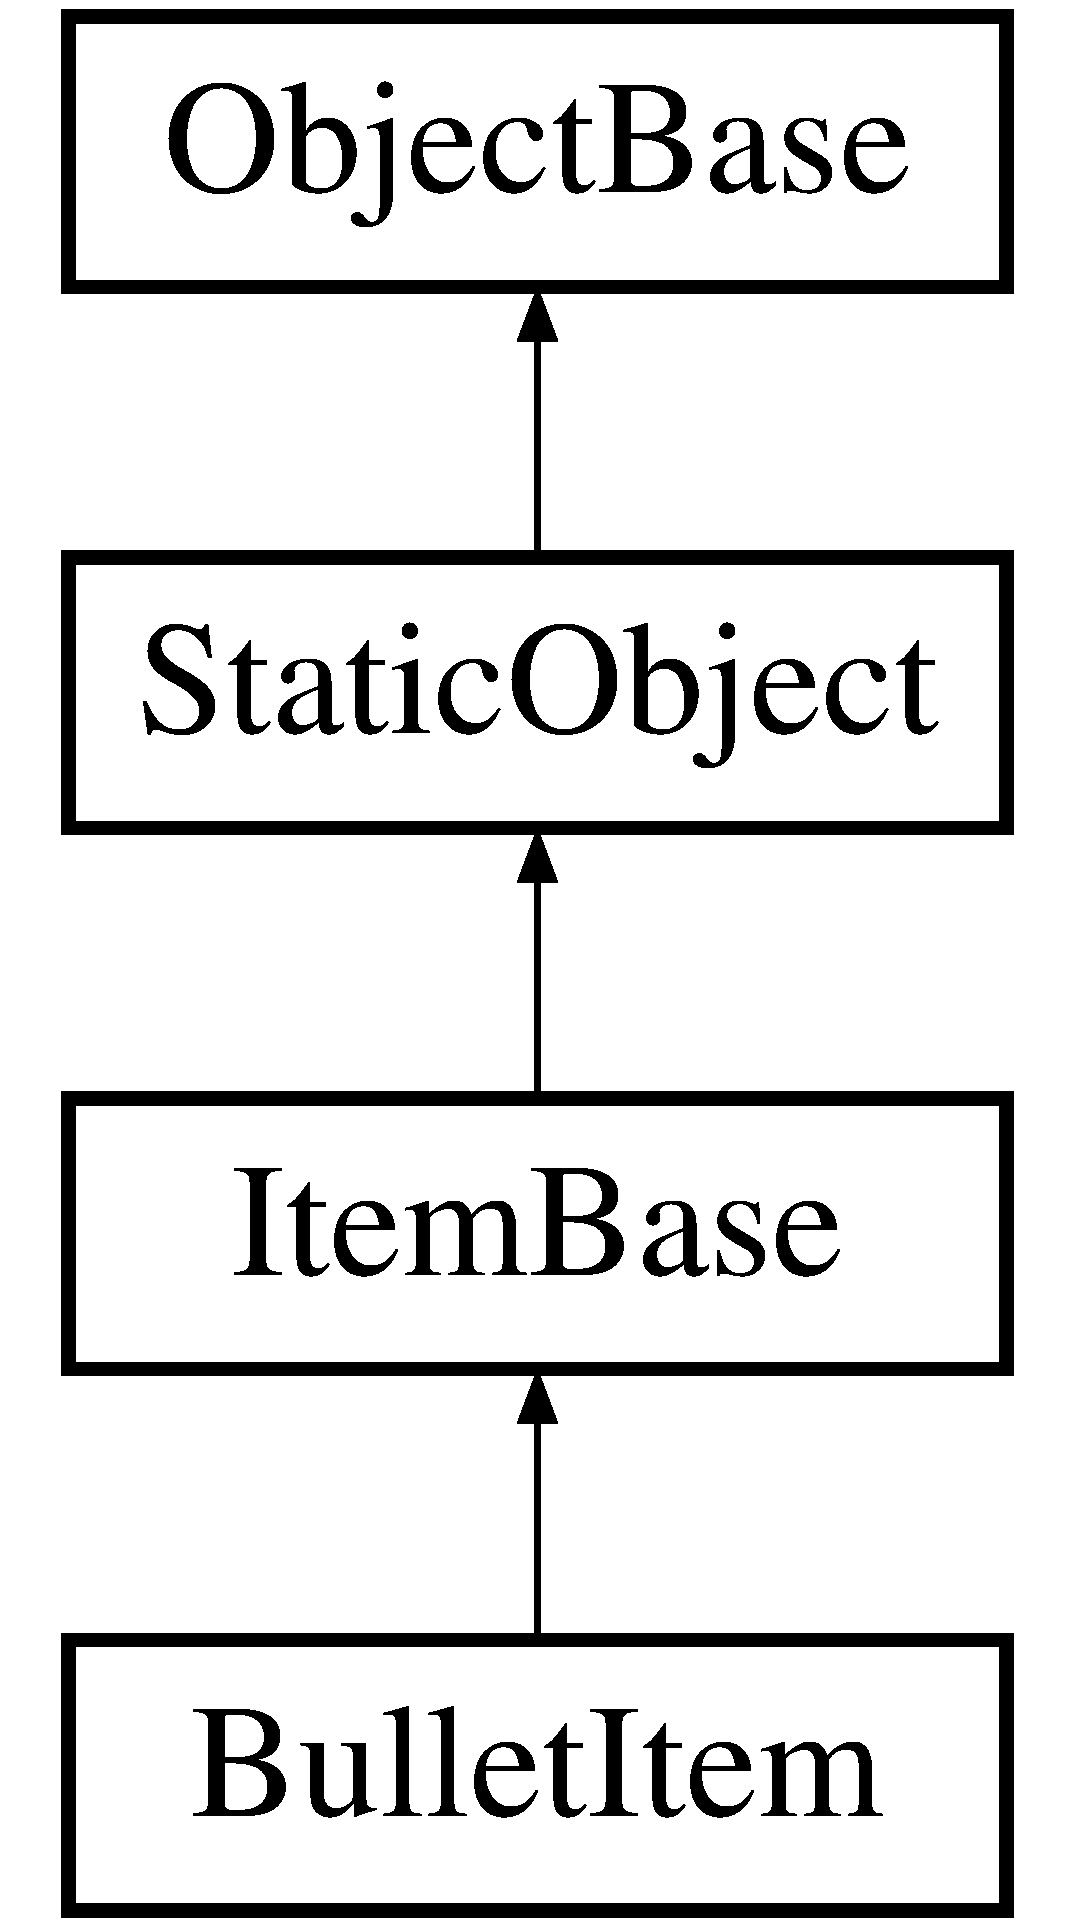
\includegraphics[height=4.000000cm]{class_item_base}
\end{center}
\end{figure}
\subsection*{公開メンバ関数}
\begin{DoxyCompactItemize}
\item 
void \mbox{\hyperlink{class_item_base_ab34d53b8f3442da77466ba1b9132386e}{Destroy}} () final
\item 
\mbox{\hyperlink{class_item_base_af005cade3ceb3329ffecd83956e4b975}{Item\+Base}} ()
\begin{DoxyCompactList}\small\item\em コンストラクタ \end{DoxyCompactList}\item 
\mbox{\hyperlink{class_item_base_a992226bfc15b036f408edf72fa94034b}{Item\+Base}} (const \mbox{\hyperlink{class_item_base}{Item\+Base}} \&m)
\begin{DoxyCompactList}\small\item\em コピーコンストラクタ \end{DoxyCompactList}\item 
\mbox{\hyperlink{class_item_base_a17a7d9d2a649e92dba8d5ee054bf10dd}{Item\+Base}} (\mbox{\hyperlink{class_item_base}{Item\+Base}} \&\&m) noexcept
\begin{DoxyCompactList}\small\item\em ムーブコンストラクタ \end{DoxyCompactList}\item 
\mbox{\hyperlink{class_item_base}{Item\+Base}} \& \mbox{\hyperlink{class_item_base_a94bf9130253e36ba8b1d4019bf5b8a3a}{operator=}} (const \mbox{\hyperlink{class_item_base}{Item\+Base}} \&other)
\begin{DoxyCompactList}\small\item\em コピー代入演算子 \end{DoxyCompactList}\item 
\mbox{\hyperlink{class_item_base}{Item\+Base}} \& \mbox{\hyperlink{class_item_base_a51a498e075511b0817ae827cdf1e3d5b}{operator=}} (\mbox{\hyperlink{class_item_base}{Item\+Base}} \&\&other) noexcept
\begin{DoxyCompactList}\small\item\em ムーブ代入演算子 \end{DoxyCompactList}\item 
\mbox{\hyperlink{class_item_base_aa3ad2e9dc1eb00a7e0e7bac7c4deb302}{$\sim$\+Item\+Base}} ()
\begin{DoxyCompactList}\small\item\em デストラクタ \end{DoxyCompactList}\item 
void \mbox{\hyperlink{class_item_base_ae5c2bcf78c74126a6f76783ca927c7ab}{Collision}} (\mbox{\hyperlink{class_object_base}{Object\+Base}} $\ast$obj, \mbox{\hyperlink{common_8h_ae148fff5818e9444b4ab2288829559bf}{Vec2}}) final
\end{DoxyCompactItemize}
\subsection*{限定公開メンバ関数}
\begin{DoxyCompactItemize}
\item 
void \mbox{\hyperlink{class_item_base_a772804cb3c663b35e44d49913d1f1cef}{Init\+Process}} () final
\item 
void \mbox{\hyperlink{class_item_base_a8edff8edcf884f9590f973fd05d218bc}{Update\+Process}} () final
\end{DoxyCompactItemize}
\subsection*{その他の継承メンバ}


\subsection{構築子と解体子}
\mbox{\Hypertarget{class_item_base_af005cade3ceb3329ffecd83956e4b975}\label{class_item_base_af005cade3ceb3329ffecd83956e4b975}} 
\index{Item\+Base@{Item\+Base}!Item\+Base@{Item\+Base}}
\index{Item\+Base@{Item\+Base}!Item\+Base@{Item\+Base}}
\subsubsection{\texorpdfstring{Item\+Base()}{ItemBase()}\hspace{0.1cm}{\footnotesize\ttfamily [1/3]}}
{\footnotesize\ttfamily Item\+Base\+::\+Item\+Base (\begin{DoxyParamCaption}{ }\end{DoxyParamCaption})\hspace{0.3cm}{\ttfamily [inline]}}



コンストラクタ 

\mbox{\Hypertarget{class_item_base_a992226bfc15b036f408edf72fa94034b}\label{class_item_base_a992226bfc15b036f408edf72fa94034b}} 
\index{Item\+Base@{Item\+Base}!Item\+Base@{Item\+Base}}
\index{Item\+Base@{Item\+Base}!Item\+Base@{Item\+Base}}
\subsubsection{\texorpdfstring{Item\+Base()}{ItemBase()}\hspace{0.1cm}{\footnotesize\ttfamily [2/3]}}
{\footnotesize\ttfamily Item\+Base\+::\+Item\+Base (\begin{DoxyParamCaption}\item[{const \mbox{\hyperlink{class_item_base}{Item\+Base}} \&}]{m }\end{DoxyParamCaption})\hspace{0.3cm}{\ttfamily [inline]}}



コピーコンストラクタ 

\mbox{\Hypertarget{class_item_base_a17a7d9d2a649e92dba8d5ee054bf10dd}\label{class_item_base_a17a7d9d2a649e92dba8d5ee054bf10dd}} 
\index{Item\+Base@{Item\+Base}!Item\+Base@{Item\+Base}}
\index{Item\+Base@{Item\+Base}!Item\+Base@{Item\+Base}}
\subsubsection{\texorpdfstring{Item\+Base()}{ItemBase()}\hspace{0.1cm}{\footnotesize\ttfamily [3/3]}}
{\footnotesize\ttfamily Item\+Base\+::\+Item\+Base (\begin{DoxyParamCaption}\item[{\mbox{\hyperlink{class_item_base}{Item\+Base}} \&\&}]{m }\end{DoxyParamCaption})\hspace{0.3cm}{\ttfamily [inline]}, {\ttfamily [noexcept]}}



ムーブコンストラクタ 

\mbox{\Hypertarget{class_item_base_aa3ad2e9dc1eb00a7e0e7bac7c4deb302}\label{class_item_base_aa3ad2e9dc1eb00a7e0e7bac7c4deb302}} 
\index{Item\+Base@{Item\+Base}!````~Item\+Base@{$\sim$\+Item\+Base}}
\index{````~Item\+Base@{$\sim$\+Item\+Base}!Item\+Base@{Item\+Base}}
\subsubsection{\texorpdfstring{$\sim$\+Item\+Base()}{~ItemBase()}}
{\footnotesize\ttfamily Item\+Base\+::$\sim$\+Item\+Base (\begin{DoxyParamCaption}{ }\end{DoxyParamCaption})\hspace{0.3cm}{\ttfamily [inline]}}



デストラクタ 



\subsection{関数詳解}
\mbox{\Hypertarget{class_item_base_ae5c2bcf78c74126a6f76783ca927c7ab}\label{class_item_base_ae5c2bcf78c74126a6f76783ca927c7ab}} 
\index{Item\+Base@{Item\+Base}!Collision@{Collision}}
\index{Collision@{Collision}!Item\+Base@{Item\+Base}}
\subsubsection{\texorpdfstring{Collision()}{Collision()}}
{\footnotesize\ttfamily void Item\+Base\+::\+Collision (\begin{DoxyParamCaption}\item[{\mbox{\hyperlink{class_object_base}{Object\+Base}} $\ast$}]{obj,  }\item[{\mbox{\hyperlink{common_8h_ae148fff5818e9444b4ab2288829559bf}{Vec2}}}]{ }\end{DoxyParamCaption})\hspace{0.3cm}{\ttfamily [inline]}, {\ttfamily [final]}, {\ttfamily [virtual]}}



\mbox{\hyperlink{class_static_object_a64c8803ff881d578d103413e299dbf7f}{Static\+Object}}を再実装しています。

\mbox{\Hypertarget{class_item_base_ab34d53b8f3442da77466ba1b9132386e}\label{class_item_base_ab34d53b8f3442da77466ba1b9132386e}} 
\index{Item\+Base@{Item\+Base}!Destroy@{Destroy}}
\index{Destroy@{Destroy}!Item\+Base@{Item\+Base}}
\subsubsection{\texorpdfstring{Destroy()}{Destroy()}}
{\footnotesize\ttfamily void Item\+Base\+::\+Destroy (\begin{DoxyParamCaption}{ }\end{DoxyParamCaption})\hspace{0.3cm}{\ttfamily [inline]}, {\ttfamily [final]}, {\ttfamily [virtual]}}



\mbox{\hyperlink{class_static_object_a8e9fb321b4f8f12c4bec1bc66853512f}{Static\+Object}}を再実装しています。

\mbox{\Hypertarget{class_item_base_a772804cb3c663b35e44d49913d1f1cef}\label{class_item_base_a772804cb3c663b35e44d49913d1f1cef}} 
\index{Item\+Base@{Item\+Base}!Init\+Process@{Init\+Process}}
\index{Init\+Process@{Init\+Process}!Item\+Base@{Item\+Base}}
\subsubsection{\texorpdfstring{Init\+Process()}{InitProcess()}}
{\footnotesize\ttfamily void Item\+Base\+::\+Init\+Process (\begin{DoxyParamCaption}{ }\end{DoxyParamCaption})\hspace{0.3cm}{\ttfamily [inline]}, {\ttfamily [final]}, {\ttfamily [protected]}, {\ttfamily [virtual]}}



\mbox{\hyperlink{class_static_object_afa0709f50495338a23c1140062a567af}{Static\+Object}}を再実装しています。

\mbox{\Hypertarget{class_item_base_a94bf9130253e36ba8b1d4019bf5b8a3a}\label{class_item_base_a94bf9130253e36ba8b1d4019bf5b8a3a}} 
\index{Item\+Base@{Item\+Base}!operator=@{operator=}}
\index{operator=@{operator=}!Item\+Base@{Item\+Base}}
\subsubsection{\texorpdfstring{operator=()}{operator=()}\hspace{0.1cm}{\footnotesize\ttfamily [1/2]}}
{\footnotesize\ttfamily \mbox{\hyperlink{class_item_base}{Item\+Base}}\& Item\+Base\+::operator= (\begin{DoxyParamCaption}\item[{const \mbox{\hyperlink{class_item_base}{Item\+Base}} \&}]{other }\end{DoxyParamCaption})\hspace{0.3cm}{\ttfamily [inline]}}



コピー代入演算子 

\mbox{\Hypertarget{class_item_base_a51a498e075511b0817ae827cdf1e3d5b}\label{class_item_base_a51a498e075511b0817ae827cdf1e3d5b}} 
\index{Item\+Base@{Item\+Base}!operator=@{operator=}}
\index{operator=@{operator=}!Item\+Base@{Item\+Base}}
\subsubsection{\texorpdfstring{operator=()}{operator=()}\hspace{0.1cm}{\footnotesize\ttfamily [2/2]}}
{\footnotesize\ttfamily \mbox{\hyperlink{class_item_base}{Item\+Base}}\& Item\+Base\+::operator= (\begin{DoxyParamCaption}\item[{\mbox{\hyperlink{class_item_base}{Item\+Base}} \&\&}]{other }\end{DoxyParamCaption})\hspace{0.3cm}{\ttfamily [inline]}, {\ttfamily [noexcept]}}



ムーブ代入演算子 

\mbox{\Hypertarget{class_item_base_a8edff8edcf884f9590f973fd05d218bc}\label{class_item_base_a8edff8edcf884f9590f973fd05d218bc}} 
\index{Item\+Base@{Item\+Base}!Update\+Process@{Update\+Process}}
\index{Update\+Process@{Update\+Process}!Item\+Base@{Item\+Base}}
\subsubsection{\texorpdfstring{Update\+Process()}{UpdateProcess()}}
{\footnotesize\ttfamily void Item\+Base\+::\+Update\+Process (\begin{DoxyParamCaption}{ }\end{DoxyParamCaption})\hspace{0.3cm}{\ttfamily [inline]}, {\ttfamily [final]}, {\ttfamily [protected]}, {\ttfamily [virtual]}}



\mbox{\hyperlink{class_static_object_a7fa678c3c4032bb6e9417f93a8bb895c}{Static\+Object}}を再実装しています。



このクラス詳解は次のファイルから抽出されました\+:\begin{DoxyCompactItemize}
\item 
C\+:/\+Users/tokir/\+Documents/\+Git\+Hub/\+Weapon\+Merchant\+Adventure/src/src/object/item/base/\mbox{\hyperlink{item__base_8h}{item\+\_\+base.\+h}}\end{DoxyCompactItemize}

\hypertarget{class_keyboard_input}{}\section{Keyboard\+Input クラス}
\label{class_keyboard_input}\index{Keyboard\+Input@{Keyboard\+Input}}


{\ttfamily \#include $<$keyboard\+\_\+input.\+h$>$}

Keyboard\+Input の継承関係図\begin{figure}[H]
\begin{center}
\leavevmode
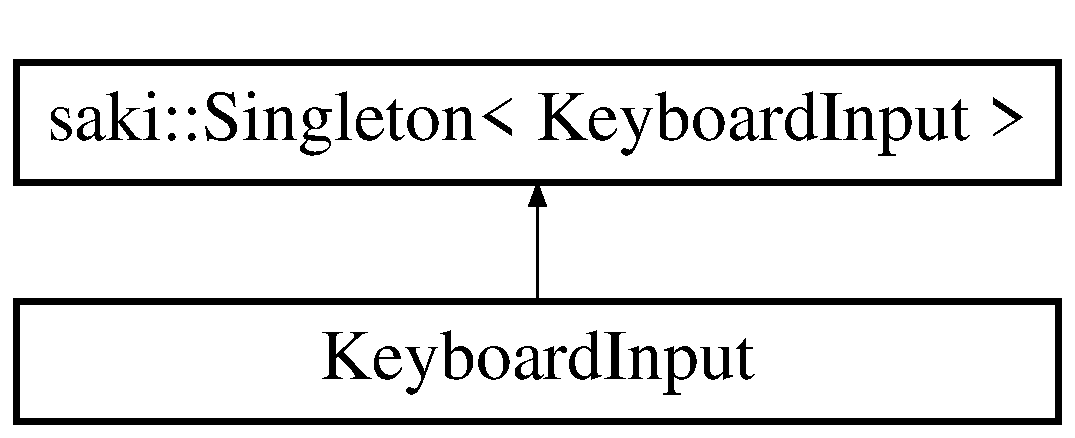
\includegraphics[height=2.000000cm]{class_keyboard_input}
\end{center}
\end{figure}
\subsection*{公開メンバ関数}
\begin{DoxyCompactItemize}
\item 
H\+R\+E\+S\+U\+LT \mbox{\hyperlink{class_keyboard_input_a89e4682682d489e35a73b641a497500c}{Keyboard\+Init}} (H\+W\+ND)
\item 
H\+R\+E\+S\+U\+LT \mbox{\hyperlink{class_keyboard_input_aa185427bfe9156eb21b12aebced6ba81}{Update}} ()
\item 
bool \mbox{\hyperlink{class_keyboard_input_a14966ce798855de8fc79432cabe7fa7b}{Get\+Key}} (int)
\item 
bool \mbox{\hyperlink{class_keyboard_input_aa3e1123287f6e473f6fda0a7af02b148}{Get\+Key\+Down}} (int)
\item 
bool \mbox{\hyperlink{class_keyboard_input_a7d1fc769524aa689c77e347091447b53}{Get\+Key\+Up}} (int)
\item 
\mbox{\hyperlink{class_keyboard_input_a2aa6da03ad4f06f93a2a940ee59d05f9}{$\sim$\+Keyboard\+Input}} ()
\end{DoxyCompactItemize}
\subsection*{その他の継承メンバ}


\subsection{構築子と解体子}
\mbox{\Hypertarget{class_keyboard_input_a2aa6da03ad4f06f93a2a940ee59d05f9}\label{class_keyboard_input_a2aa6da03ad4f06f93a2a940ee59d05f9}} 
\index{Keyboard\+Input@{Keyboard\+Input}!````~Keyboard\+Input@{$\sim$\+Keyboard\+Input}}
\index{````~Keyboard\+Input@{$\sim$\+Keyboard\+Input}!Keyboard\+Input@{Keyboard\+Input}}
\subsubsection{\texorpdfstring{$\sim$\+Keyboard\+Input()}{~KeyboardInput()}}
{\footnotesize\ttfamily Keyboard\+Input\+::$\sim$\+Keyboard\+Input (\begin{DoxyParamCaption}{ }\end{DoxyParamCaption})\hspace{0.3cm}{\ttfamily [inline]}}



\subsection{関数詳解}
\mbox{\Hypertarget{class_keyboard_input_a14966ce798855de8fc79432cabe7fa7b}\label{class_keyboard_input_a14966ce798855de8fc79432cabe7fa7b}} 
\index{Keyboard\+Input@{Keyboard\+Input}!Get\+Key@{Get\+Key}}
\index{Get\+Key@{Get\+Key}!Keyboard\+Input@{Keyboard\+Input}}
\subsubsection{\texorpdfstring{Get\+Key()}{GetKey()}}
{\footnotesize\ttfamily bool Keyboard\+Input\+::\+Get\+Key (\begin{DoxyParamCaption}\item[{int}]{key }\end{DoxyParamCaption})}

\mbox{\Hypertarget{class_keyboard_input_aa3e1123287f6e473f6fda0a7af02b148}\label{class_keyboard_input_aa3e1123287f6e473f6fda0a7af02b148}} 
\index{Keyboard\+Input@{Keyboard\+Input}!Get\+Key\+Down@{Get\+Key\+Down}}
\index{Get\+Key\+Down@{Get\+Key\+Down}!Keyboard\+Input@{Keyboard\+Input}}
\subsubsection{\texorpdfstring{Get\+Key\+Down()}{GetKeyDown()}}
{\footnotesize\ttfamily bool Keyboard\+Input\+::\+Get\+Key\+Down (\begin{DoxyParamCaption}\item[{int}]{key }\end{DoxyParamCaption})}

\mbox{\Hypertarget{class_keyboard_input_a7d1fc769524aa689c77e347091447b53}\label{class_keyboard_input_a7d1fc769524aa689c77e347091447b53}} 
\index{Keyboard\+Input@{Keyboard\+Input}!Get\+Key\+Up@{Get\+Key\+Up}}
\index{Get\+Key\+Up@{Get\+Key\+Up}!Keyboard\+Input@{Keyboard\+Input}}
\subsubsection{\texorpdfstring{Get\+Key\+Up()}{GetKeyUp()}}
{\footnotesize\ttfamily bool Keyboard\+Input\+::\+Get\+Key\+Up (\begin{DoxyParamCaption}\item[{int}]{key }\end{DoxyParamCaption})}

\mbox{\Hypertarget{class_keyboard_input_a89e4682682d489e35a73b641a497500c}\label{class_keyboard_input_a89e4682682d489e35a73b641a497500c}} 
\index{Keyboard\+Input@{Keyboard\+Input}!Keyboard\+Init@{Keyboard\+Init}}
\index{Keyboard\+Init@{Keyboard\+Init}!Keyboard\+Input@{Keyboard\+Input}}
\subsubsection{\texorpdfstring{Keyboard\+Init()}{KeyboardInit()}}
{\footnotesize\ttfamily H\+R\+E\+S\+U\+LT Keyboard\+Input\+::\+Keyboard\+Init (\begin{DoxyParamCaption}\item[{H\+W\+ND}]{h\+Wnd }\end{DoxyParamCaption})}

\mbox{\Hypertarget{class_keyboard_input_aa185427bfe9156eb21b12aebced6ba81}\label{class_keyboard_input_aa185427bfe9156eb21b12aebced6ba81}} 
\index{Keyboard\+Input@{Keyboard\+Input}!Update@{Update}}
\index{Update@{Update}!Keyboard\+Input@{Keyboard\+Input}}
\subsubsection{\texorpdfstring{Update()}{Update()}}
{\footnotesize\ttfamily H\+R\+E\+S\+U\+LT Keyboard\+Input\+::\+Update (\begin{DoxyParamCaption}{ }\end{DoxyParamCaption})}



このクラス詳解は次のファイルから抽出されました\+:\begin{DoxyCompactItemize}
\item 
C\+:/\+Users/tokir/\+Documents/\+Git\+Hub/\+Weapon\+Merchant\+Adventure/src/src/input/keyboard/\mbox{\hyperlink{keyboard__input_8h}{keyboard\+\_\+input.\+h}}\item 
C\+:/\+Users/tokir/\+Documents/\+Git\+Hub/\+Weapon\+Merchant\+Adventure/src/src/input/keyboard/\mbox{\hyperlink{keyboard__input_8cpp}{keyboard\+\_\+input.\+cpp}}\end{DoxyCompactItemize}

\hypertarget{class_load_map}{}\section{Load\+Map クラス}
\label{class_load_map}\index{Load\+Map@{Load\+Map}}


マップロードクラス  




{\ttfamily \#include $<$load\+\_\+map.\+h$>$}

Load\+Map の継承関係図\begin{figure}[H]
\begin{center}
\leavevmode
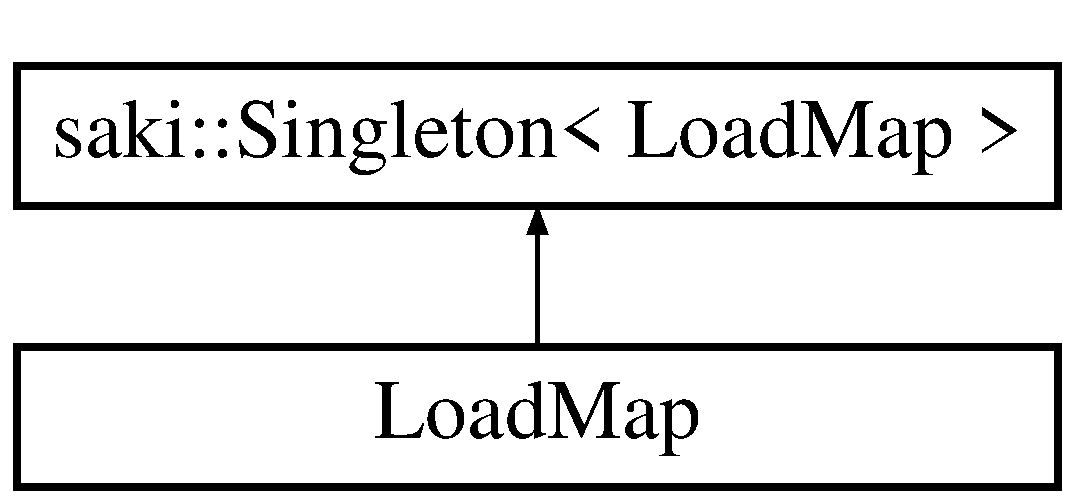
\includegraphics[height=2.000000cm]{class_load_map}
\end{center}
\end{figure}
\subsection*{公開メンバ関数}
\begin{DoxyCompactItemize}
\item 
void \mbox{\hyperlink{class_load_map_a534a2ac8151a7549b1fed723759ab2d0}{Game\+Loading\+Map}} (W\+C\+H\+AR $\ast$, W\+C\+H\+AR $\ast$)
\begin{DoxyCompactList}\small\item\em ゲームマップの読み込み \end{DoxyCompactList}\item 
void \mbox{\hyperlink{class_load_map_a44d4c9299837322a7eedbb298b6dbda9}{Game\+Making\+Map}} (std\+::vector$<$ \mbox{\hyperlink{class_map_object}{Map\+Object}} $>$ \&, std\+::list$<$ \mbox{\hyperlink{class_normal_enemy}{Normal\+Enemy}} $>$ \&, std\+::list$<$ \mbox{\hyperlink{class_fly_enemy}{Fly\+Enemy}} $>$ \&, std\+::unique\+\_\+ptr$<$ \mbox{\hyperlink{class_boss}{Boss}} $>$ \&, std\+::unique\+\_\+ptr$<$ \mbox{\hyperlink{class_player}{Player}} $>$ \&, std\+::list$<$ \mbox{\hyperlink{class_bullet_item}{Bullet\+Item}} $>$ \&)
\begin{DoxyCompactList}\small\item\em ゲームマップの作成 \end{DoxyCompactList}\item 
void \mbox{\hyperlink{class_load_map_a9cfbf3d52bcaf5384d882c1cf591bf43}{Title\+Select\+Loading\+Map}} (W\+C\+H\+AR $\ast$)
\begin{DoxyCompactList}\small\item\em タイトルかセレクトマップの読み込み \end{DoxyCompactList}\item 
void \mbox{\hyperlink{class_load_map_a69d69c3ac701f152395a18719c16c881}{Title\+Select\+Making\+Map}} (std\+::vector$<$ \mbox{\hyperlink{class_map_object}{Map\+Object}} $>$ \&, std\+::unique\+\_\+ptr$<$ \mbox{\hyperlink{class_player}{Player}} $>$ \&, std\+::vector$<$ \mbox{\hyperlink{class_select_obj}{Select\+Obj}} $>$ \&, \mbox{\hyperlink{class_static_object}{Static\+Object}} \&)
\begin{DoxyCompactList}\small\item\em ゲームマップの作成 \end{DoxyCompactList}\end{DoxyCompactItemize}
\subsection*{その他の継承メンバ}


\subsection{詳解}
マップロードクラス 

\subsection{関数詳解}
\mbox{\Hypertarget{class_load_map_a534a2ac8151a7549b1fed723759ab2d0}\label{class_load_map_a534a2ac8151a7549b1fed723759ab2d0}} 
\index{Load\+Map@{Load\+Map}!Game\+Loading\+Map@{Game\+Loading\+Map}}
\index{Game\+Loading\+Map@{Game\+Loading\+Map}!Load\+Map@{Load\+Map}}
\subsubsection{\texorpdfstring{Game\+Loading\+Map()}{GameLoadingMap()}}
{\footnotesize\ttfamily void Load\+Map\+::\+Game\+Loading\+Map (\begin{DoxyParamCaption}\item[{W\+C\+H\+AR $\ast$}]{r\+\_\+map\+\_\+path,  }\item[{W\+C\+H\+AR $\ast$}]{r\+\_\+fly\+\_\+path }\end{DoxyParamCaption})}



ゲームマップの読み込み 


\begin{DoxyParams}{引数}
{\em r\+\_\+map\+\_\+path} & 読み込むマップcsvのパス \\
\hline
{\em r\+\_\+flu\+\_\+path} & 読み込む飛ぶ鳥csvのパス \\
\hline
\end{DoxyParams}
\mbox{\Hypertarget{class_load_map_a44d4c9299837322a7eedbb298b6dbda9}\label{class_load_map_a44d4c9299837322a7eedbb298b6dbda9}} 
\index{Load\+Map@{Load\+Map}!Game\+Making\+Map@{Game\+Making\+Map}}
\index{Game\+Making\+Map@{Game\+Making\+Map}!Load\+Map@{Load\+Map}}
\subsubsection{\texorpdfstring{Game\+Making\+Map()}{GameMakingMap()}}
{\footnotesize\ttfamily void Load\+Map\+::\+Game\+Making\+Map (\begin{DoxyParamCaption}\item[{std\+::vector$<$ \mbox{\hyperlink{class_map_object}{Map\+Object}} $>$ \&}]{m,  }\item[{std\+::list$<$ \mbox{\hyperlink{class_normal_enemy}{Normal\+Enemy}} $>$ \&}]{enemy,  }\item[{std\+::list$<$ \mbox{\hyperlink{class_fly_enemy}{Fly\+Enemy}} $>$ \&}]{f\+\_\+enemy,  }\item[{std\+::unique\+\_\+ptr$<$ \mbox{\hyperlink{class_boss}{Boss}} $>$ \&}]{boss,  }\item[{std\+::unique\+\_\+ptr$<$ \mbox{\hyperlink{class_player}{Player}} $>$ \&}]{player,  }\item[{std\+::list$<$ \mbox{\hyperlink{class_bullet_item}{Bullet\+Item}} $>$ \&}]{bullet\+\_\+item }\end{DoxyParamCaption})}



ゲームマップの作成 


\begin{DoxyParams}{引数}
{\em m} & マップのstd\+::vector \\
\hline
{\em enemy} & 敵のstd\+::list \\
\hline
{\em f\+\_\+enemy} & 飛ぶ敵のstd\+::list \\
\hline
{\em boss} & ボスのstd\+::unique\+\_\+ptr \\
\hline
{\em player} & プレイヤーのstd\+::unique\+\_\+ptr \\
\hline
{\em bullet\+\_\+item} & 弾のアイテムのstd\+::list \\
\hline
\end{DoxyParams}
\mbox{\Hypertarget{class_load_map_a9cfbf3d52bcaf5384d882c1cf591bf43}\label{class_load_map_a9cfbf3d52bcaf5384d882c1cf591bf43}} 
\index{Load\+Map@{Load\+Map}!Title\+Select\+Loading\+Map@{Title\+Select\+Loading\+Map}}
\index{Title\+Select\+Loading\+Map@{Title\+Select\+Loading\+Map}!Load\+Map@{Load\+Map}}
\subsubsection{\texorpdfstring{Title\+Select\+Loading\+Map()}{TitleSelectLoadingMap()}}
{\footnotesize\ttfamily void Load\+Map\+::\+Title\+Select\+Loading\+Map (\begin{DoxyParamCaption}\item[{W\+C\+H\+AR $\ast$}]{r\+\_\+map\+\_\+path }\end{DoxyParamCaption})}



タイトルかセレクトマップの読み込み 


\begin{DoxyParams}{引数}
{\em r\+\_\+map\+\_\+path} & 読み込むマップcsvのパス \\
\hline
\end{DoxyParams}
\mbox{\Hypertarget{class_load_map_a69d69c3ac701f152395a18719c16c881}\label{class_load_map_a69d69c3ac701f152395a18719c16c881}} 
\index{Load\+Map@{Load\+Map}!Title\+Select\+Making\+Map@{Title\+Select\+Making\+Map}}
\index{Title\+Select\+Making\+Map@{Title\+Select\+Making\+Map}!Load\+Map@{Load\+Map}}
\subsubsection{\texorpdfstring{Title\+Select\+Making\+Map()}{TitleSelectMakingMap()}}
{\footnotesize\ttfamily void Load\+Map\+::\+Title\+Select\+Making\+Map (\begin{DoxyParamCaption}\item[{std\+::vector$<$ \mbox{\hyperlink{class_map_object}{Map\+Object}} $>$ \&}]{m,  }\item[{std\+::unique\+\_\+ptr$<$ \mbox{\hyperlink{class_player}{Player}} $>$ \&}]{player,  }\item[{std\+::vector$<$ \mbox{\hyperlink{class_select_obj}{Select\+Obj}} $>$ \&}]{select\+\_\+obj,  }\item[{\mbox{\hyperlink{class_static_object}{Static\+Object}} \&}]{sign }\end{DoxyParamCaption})}



ゲームマップの作成 


\begin{DoxyParams}{引数}
{\em m} & マップのstd\+::vector \\
\hline
{\em player} & プレイヤーのstd\+::unique\+\_\+ptr \\
\hline
\end{DoxyParams}


このクラス詳解は次のファイルから抽出されました\+:\begin{DoxyCompactItemize}
\item 
C\+:/\+Users/tokir/\+Documents/\+Git\+Hub/\+Weapon\+Merchant\+Adventure/src/src/load/map/\mbox{\hyperlink{load__map_8h}{load\+\_\+map.\+h}}\item 
C\+:/\+Users/tokir/\+Documents/\+Git\+Hub/\+Weapon\+Merchant\+Adventure/src/src/load/map/\mbox{\hyperlink{load__map_8cpp}{load\+\_\+map.\+cpp}}\end{DoxyCompactItemize}

\hypertarget{class_main}{}\section{Main クラス}
\label{class_main}\index{Main@{Main}}


{\ttfamily \#include $<$main.\+h$>$}

Main の継承関係図\begin{figure}[H]
\begin{center}
\leavevmode
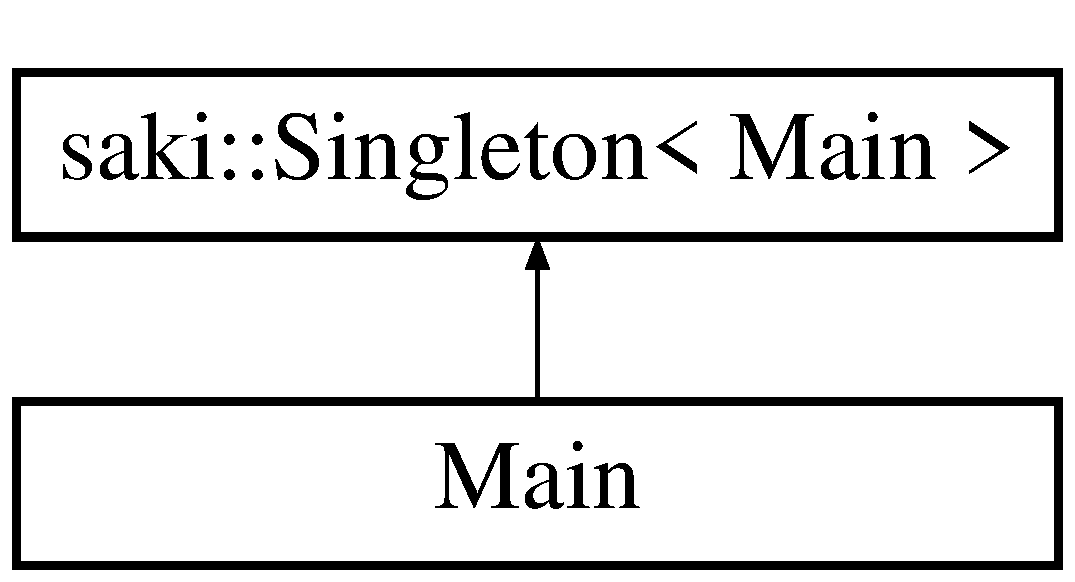
\includegraphics[height=2.000000cm]{class_main}
\end{center}
\end{figure}
\subsection*{公開メンバ関数}
\begin{DoxyCompactItemize}
\item 
H\+R\+E\+S\+U\+LT \mbox{\hyperlink{class_main_a73509ef41bc8441ce33ff8068a173f6b}{init\+\_\+window}} (H\+I\+N\+S\+T\+A\+N\+CE, int)
\end{DoxyCompactItemize}
\subsection*{公開変数類}
\begin{DoxyCompactItemize}
\item 
H\+W\+ND \mbox{\hyperlink{class_main_a511de4617f7e21d53dfa8bba5e8e40f6}{hwnd}}
\item 
H\+I\+N\+S\+T\+A\+N\+CE \mbox{\hyperlink{class_main_a7e08e3cceedf7301924454e77d6fe2b1}{hinst}}
\end{DoxyCompactItemize}
\subsection*{その他の継承メンバ}


\subsection{関数詳解}
\mbox{\Hypertarget{class_main_a73509ef41bc8441ce33ff8068a173f6b}\label{class_main_a73509ef41bc8441ce33ff8068a173f6b}} 
\index{Main@{Main}!init\+\_\+window@{init\+\_\+window}}
\index{init\+\_\+window@{init\+\_\+window}!Main@{Main}}
\subsubsection{\texorpdfstring{init\+\_\+window()}{init\_window()}}
{\footnotesize\ttfamily H\+R\+E\+S\+U\+LT Main\+::init\+\_\+window (\begin{DoxyParamCaption}\item[{H\+I\+N\+S\+T\+A\+N\+CE}]{h\+Inst,  }\item[{int}]{n\+Cmd }\end{DoxyParamCaption})}



\subsection{メンバ詳解}
\mbox{\Hypertarget{class_main_a7e08e3cceedf7301924454e77d6fe2b1}\label{class_main_a7e08e3cceedf7301924454e77d6fe2b1}} 
\index{Main@{Main}!hinst@{hinst}}
\index{hinst@{hinst}!Main@{Main}}
\subsubsection{\texorpdfstring{hinst}{hinst}}
{\footnotesize\ttfamily H\+I\+N\+S\+T\+A\+N\+CE Main\+::hinst}

\mbox{\Hypertarget{class_main_a511de4617f7e21d53dfa8bba5e8e40f6}\label{class_main_a511de4617f7e21d53dfa8bba5e8e40f6}} 
\index{Main@{Main}!hwnd@{hwnd}}
\index{hwnd@{hwnd}!Main@{Main}}
\subsubsection{\texorpdfstring{hwnd}{hwnd}}
{\footnotesize\ttfamily H\+W\+ND Main\+::hwnd}



このクラス詳解は次のファイルから抽出されました\+:\begin{DoxyCompactItemize}
\item 
C\+:/\+Users/tokir/\+Documents/\+Git\+Hub/\+Weapon\+Merchant\+Adventure/src/src/main/\mbox{\hyperlink{main_8h}{main.\+h}}\item 
C\+:/\+Users/tokir/\+Documents/\+Git\+Hub/\+Weapon\+Merchant\+Adventure/src/src/main/\mbox{\hyperlink{main_8cpp}{main.\+cpp}}\end{DoxyCompactItemize}

\hypertarget{class_map_object}{}\section{Map\+Object クラス}
\label{class_map_object}\index{Map\+Object@{Map\+Object}}


マップに配置するオブジェクトのクラス  




{\ttfamily \#include $<$map.\+h$>$}

Map\+Object の継承関係図\begin{figure}[H]
\begin{center}
\leavevmode
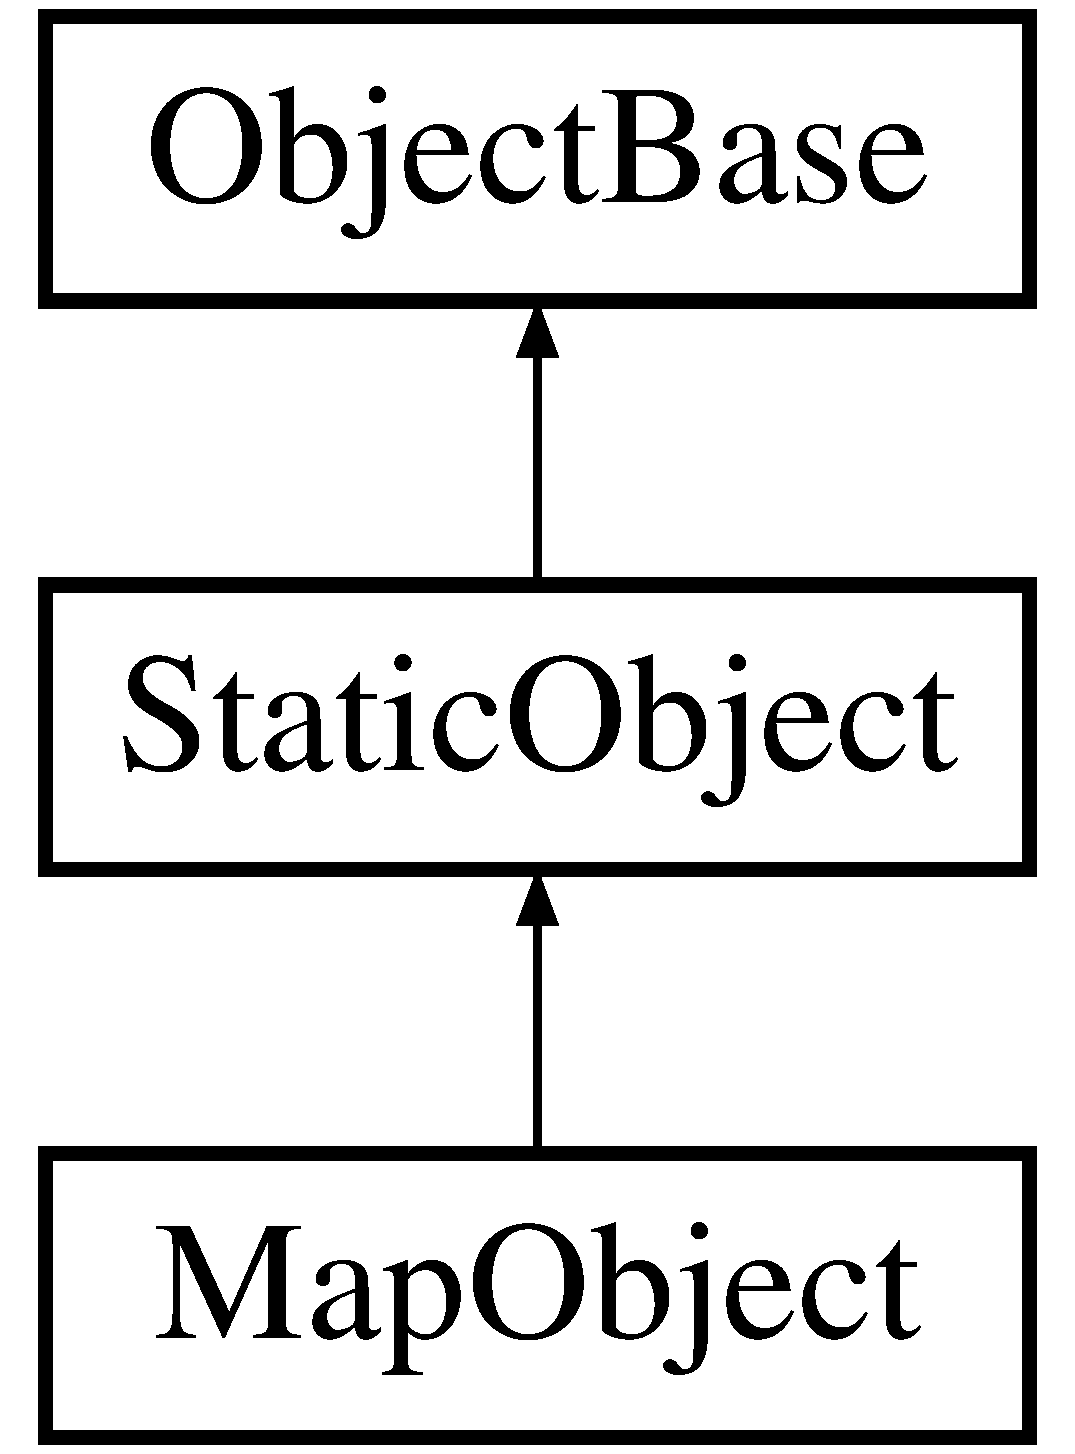
\includegraphics[height=3.000000cm]{class_map_object}
\end{center}
\end{figure}
\subsection*{公開メンバ関数}
\begin{DoxyCompactItemize}
\item 
void \mbox{\hyperlink{class_map_object_ad4bcfdc33bd945a9aa5e50a57c2704bc}{Destroy}} () final
\begin{DoxyCompactList}\small\item\em マップの破棄 \end{DoxyCompactList}\item 
\mbox{\hyperlink{class_map_object_a568754515cc72ce0861d30c3040d26d2}{Map\+Object}} ()
\begin{DoxyCompactList}\small\item\em コンストラクタ \end{DoxyCompactList}\item 
\mbox{\hyperlink{class_map_object_a4d69915b6837056e40c0c17afe78ce8e}{Map\+Object}} (const \mbox{\hyperlink{class_map_object}{Map\+Object}} \&m)
\begin{DoxyCompactList}\small\item\em コピーコンストラクタ \end{DoxyCompactList}\item 
\mbox{\hyperlink{class_map_object_ad3779307ee41c0bc0fdf4b419baac3da}{Map\+Object}} (\mbox{\hyperlink{class_map_object}{Map\+Object}} \&\&m) noexcept
\begin{DoxyCompactList}\small\item\em ムーブコンストラクタ \end{DoxyCompactList}\item 
\mbox{\hyperlink{class_map_object}{Map\+Object}} \& \mbox{\hyperlink{class_map_object_a4ff3c31cc463a650e4d870ea65b65c58}{operator=}} (const \mbox{\hyperlink{class_map_object}{Map\+Object}} \&other)
\begin{DoxyCompactList}\small\item\em コピー代入演算子 \end{DoxyCompactList}\item 
\mbox{\hyperlink{class_map_object}{Map\+Object}} \& \mbox{\hyperlink{class_map_object_ae36fa838f3f8bac8ef2d67b39adf0298}{operator=}} (\mbox{\hyperlink{class_map_object}{Map\+Object}} \&\&other) noexcept
\begin{DoxyCompactList}\small\item\em ムーブ代入演算子 \end{DoxyCompactList}\item 
void \mbox{\hyperlink{class_map_object_a76b9161f2723272ad361d0b190e46245}{Collision}} (\mbox{\hyperlink{class_object_base}{Object\+Base}} $\ast$, \mbox{\hyperlink{common_8h_ae148fff5818e9444b4ab2288829559bf}{Vec2}}) final
\begin{DoxyCompactList}\small\item\em マップが当たってるときに実行する関数 \end{DoxyCompactList}\item 
\mbox{\hyperlink{class_map_object_aa601344267a49df197e841fcbd732209}{$\sim$\+Map\+Object}} ()
\begin{DoxyCompactList}\small\item\em デストラクタ \end{DoxyCompactList}\end{DoxyCompactItemize}
\subsection*{公開変数類}
\begin{DoxyCompactItemize}
\item 
bool \mbox{\hyperlink{class_map_object_a21c5d70f23cca2a184297d766cc6acdc}{is\+\_\+mapchip}} = true
\end{DoxyCompactItemize}
\subsection*{限定公開メンバ関数}
\begin{DoxyCompactItemize}
\item 
void \mbox{\hyperlink{class_map_object_a3043cddb8aaad0eab27a076e9bee0284}{Init\+Process}} () final
\begin{DoxyCompactList}\small\item\em 初期化 \end{DoxyCompactList}\item 
void \mbox{\hyperlink{class_map_object_ab6b8849f15175417eca94b2703945e4b}{Update\+Process}} () final
\begin{DoxyCompactList}\small\item\em マップの更新 \end{DoxyCompactList}\end{DoxyCompactItemize}
\subsection*{その他の継承メンバ}


\subsection{詳解}
マップに配置するオブジェクトのクラス 

\subsection{構築子と解体子}
\mbox{\Hypertarget{class_map_object_a568754515cc72ce0861d30c3040d26d2}\label{class_map_object_a568754515cc72ce0861d30c3040d26d2}} 
\index{Map\+Object@{Map\+Object}!Map\+Object@{Map\+Object}}
\index{Map\+Object@{Map\+Object}!Map\+Object@{Map\+Object}}
\subsubsection{\texorpdfstring{Map\+Object()}{MapObject()}\hspace{0.1cm}{\footnotesize\ttfamily [1/3]}}
{\footnotesize\ttfamily Map\+Object\+::\+Map\+Object (\begin{DoxyParamCaption}{ }\end{DoxyParamCaption})\hspace{0.3cm}{\ttfamily [inline]}}



コンストラクタ 

\mbox{\Hypertarget{class_map_object_a4d69915b6837056e40c0c17afe78ce8e}\label{class_map_object_a4d69915b6837056e40c0c17afe78ce8e}} 
\index{Map\+Object@{Map\+Object}!Map\+Object@{Map\+Object}}
\index{Map\+Object@{Map\+Object}!Map\+Object@{Map\+Object}}
\subsubsection{\texorpdfstring{Map\+Object()}{MapObject()}\hspace{0.1cm}{\footnotesize\ttfamily [2/3]}}
{\footnotesize\ttfamily Map\+Object\+::\+Map\+Object (\begin{DoxyParamCaption}\item[{const \mbox{\hyperlink{class_map_object}{Map\+Object}} \&}]{m }\end{DoxyParamCaption})\hspace{0.3cm}{\ttfamily [inline]}}



コピーコンストラクタ 

\mbox{\Hypertarget{class_map_object_ad3779307ee41c0bc0fdf4b419baac3da}\label{class_map_object_ad3779307ee41c0bc0fdf4b419baac3da}} 
\index{Map\+Object@{Map\+Object}!Map\+Object@{Map\+Object}}
\index{Map\+Object@{Map\+Object}!Map\+Object@{Map\+Object}}
\subsubsection{\texorpdfstring{Map\+Object()}{MapObject()}\hspace{0.1cm}{\footnotesize\ttfamily [3/3]}}
{\footnotesize\ttfamily Map\+Object\+::\+Map\+Object (\begin{DoxyParamCaption}\item[{\mbox{\hyperlink{class_map_object}{Map\+Object}} \&\&}]{m }\end{DoxyParamCaption})\hspace{0.3cm}{\ttfamily [inline]}, {\ttfamily [noexcept]}}



ムーブコンストラクタ 

\mbox{\Hypertarget{class_map_object_aa601344267a49df197e841fcbd732209}\label{class_map_object_aa601344267a49df197e841fcbd732209}} 
\index{Map\+Object@{Map\+Object}!````~Map\+Object@{$\sim$\+Map\+Object}}
\index{````~Map\+Object@{$\sim$\+Map\+Object}!Map\+Object@{Map\+Object}}
\subsubsection{\texorpdfstring{$\sim$\+Map\+Object()}{~MapObject()}}
{\footnotesize\ttfamily Map\+Object\+::$\sim$\+Map\+Object (\begin{DoxyParamCaption}{ }\end{DoxyParamCaption})\hspace{0.3cm}{\ttfamily [inline]}}



デストラクタ 



\subsection{関数詳解}
\mbox{\Hypertarget{class_map_object_a76b9161f2723272ad361d0b190e46245}\label{class_map_object_a76b9161f2723272ad361d0b190e46245}} 
\index{Map\+Object@{Map\+Object}!Collision@{Collision}}
\index{Collision@{Collision}!Map\+Object@{Map\+Object}}
\subsubsection{\texorpdfstring{Collision()}{Collision()}}
{\footnotesize\ttfamily void Map\+Object\+::\+Collision (\begin{DoxyParamCaption}\item[{\mbox{\hyperlink{class_object_base}{Object\+Base}} $\ast$}]{obj,  }\item[{\mbox{\hyperlink{common_8h_ae148fff5818e9444b4ab2288829559bf}{Vec2}}}]{ }\end{DoxyParamCaption})\hspace{0.3cm}{\ttfamily [final]}, {\ttfamily [virtual]}}



マップが当たってるときに実行する関数 



\mbox{\hyperlink{class_static_object_a64c8803ff881d578d103413e299dbf7f}{Static\+Object}}を再実装しています。

\mbox{\Hypertarget{class_map_object_ad4bcfdc33bd945a9aa5e50a57c2704bc}\label{class_map_object_ad4bcfdc33bd945a9aa5e50a57c2704bc}} 
\index{Map\+Object@{Map\+Object}!Destroy@{Destroy}}
\index{Destroy@{Destroy}!Map\+Object@{Map\+Object}}
\subsubsection{\texorpdfstring{Destroy()}{Destroy()}}
{\footnotesize\ttfamily void Map\+Object\+::\+Destroy (\begin{DoxyParamCaption}{ }\end{DoxyParamCaption})\hspace{0.3cm}{\ttfamily [final]}, {\ttfamily [virtual]}}



マップの破棄 



\mbox{\hyperlink{class_static_object_a8e9fb321b4f8f12c4bec1bc66853512f}{Static\+Object}}を再実装しています。

\mbox{\Hypertarget{class_map_object_a3043cddb8aaad0eab27a076e9bee0284}\label{class_map_object_a3043cddb8aaad0eab27a076e9bee0284}} 
\index{Map\+Object@{Map\+Object}!Init\+Process@{Init\+Process}}
\index{Init\+Process@{Init\+Process}!Map\+Object@{Map\+Object}}
\subsubsection{\texorpdfstring{Init\+Process()}{InitProcess()}}
{\footnotesize\ttfamily void Map\+Object\+::\+Init\+Process (\begin{DoxyParamCaption}{ }\end{DoxyParamCaption})\hspace{0.3cm}{\ttfamily [final]}, {\ttfamily [protected]}, {\ttfamily [virtual]}}



初期化 



\mbox{\hyperlink{class_static_object_afa0709f50495338a23c1140062a567af}{Static\+Object}}を再実装しています。

\mbox{\Hypertarget{class_map_object_a4ff3c31cc463a650e4d870ea65b65c58}\label{class_map_object_a4ff3c31cc463a650e4d870ea65b65c58}} 
\index{Map\+Object@{Map\+Object}!operator=@{operator=}}
\index{operator=@{operator=}!Map\+Object@{Map\+Object}}
\subsubsection{\texorpdfstring{operator=()}{operator=()}\hspace{0.1cm}{\footnotesize\ttfamily [1/2]}}
{\footnotesize\ttfamily \mbox{\hyperlink{class_map_object}{Map\+Object}}\& Map\+Object\+::operator= (\begin{DoxyParamCaption}\item[{const \mbox{\hyperlink{class_map_object}{Map\+Object}} \&}]{other }\end{DoxyParamCaption})\hspace{0.3cm}{\ttfamily [inline]}}



コピー代入演算子 

\mbox{\Hypertarget{class_map_object_ae36fa838f3f8bac8ef2d67b39adf0298}\label{class_map_object_ae36fa838f3f8bac8ef2d67b39adf0298}} 
\index{Map\+Object@{Map\+Object}!operator=@{operator=}}
\index{operator=@{operator=}!Map\+Object@{Map\+Object}}
\subsubsection{\texorpdfstring{operator=()}{operator=()}\hspace{0.1cm}{\footnotesize\ttfamily [2/2]}}
{\footnotesize\ttfamily \mbox{\hyperlink{class_map_object}{Map\+Object}}\& Map\+Object\+::operator= (\begin{DoxyParamCaption}\item[{\mbox{\hyperlink{class_map_object}{Map\+Object}} \&\&}]{other }\end{DoxyParamCaption})\hspace{0.3cm}{\ttfamily [inline]}, {\ttfamily [noexcept]}}



ムーブ代入演算子 

\mbox{\Hypertarget{class_map_object_ab6b8849f15175417eca94b2703945e4b}\label{class_map_object_ab6b8849f15175417eca94b2703945e4b}} 
\index{Map\+Object@{Map\+Object}!Update\+Process@{Update\+Process}}
\index{Update\+Process@{Update\+Process}!Map\+Object@{Map\+Object}}
\subsubsection{\texorpdfstring{Update\+Process()}{UpdateProcess()}}
{\footnotesize\ttfamily void Map\+Object\+::\+Update\+Process (\begin{DoxyParamCaption}{ }\end{DoxyParamCaption})\hspace{0.3cm}{\ttfamily [final]}, {\ttfamily [protected]}, {\ttfamily [virtual]}}



マップの更新 



\mbox{\hyperlink{class_static_object_a7fa678c3c4032bb6e9417f93a8bb895c}{Static\+Object}}を再実装しています。



\subsection{メンバ詳解}
\mbox{\Hypertarget{class_map_object_a21c5d70f23cca2a184297d766cc6acdc}\label{class_map_object_a21c5d70f23cca2a184297d766cc6acdc}} 
\index{Map\+Object@{Map\+Object}!is\+\_\+mapchip@{is\+\_\+mapchip}}
\index{is\+\_\+mapchip@{is\+\_\+mapchip}!Map\+Object@{Map\+Object}}
\subsubsection{\texorpdfstring{is\+\_\+mapchip}{is\_mapchip}}
{\footnotesize\ttfamily bool Map\+Object\+::is\+\_\+mapchip = true}



このクラス詳解は次のファイルから抽出されました\+:\begin{DoxyCompactItemize}
\item 
C\+:/\+Users/tokir/\+Documents/\+Git\+Hub/\+Weapon\+Merchant\+Adventure/src/src/object/map/\mbox{\hyperlink{map_8h}{map.\+h}}\item 
C\+:/\+Users/tokir/\+Documents/\+Git\+Hub/\+Weapon\+Merchant\+Adventure/src/src/object/map/\mbox{\hyperlink{map_8cpp}{map.\+cpp}}\end{DoxyCompactItemize}

\hypertarget{classsaki_1_1_matrix}{}\section{saki\+:\+:Matrix$<$ T $>$ クラステンプレート}
\label{classsaki_1_1_matrix}\index{saki\+::\+Matrix$<$ T $>$@{saki\+::\+Matrix$<$ T $>$}}


行列  




{\ttfamily \#include $<$matrix\+\_\+operator.\+h$>$}

\subsection*{公開メンバ関数}
\begin{DoxyCompactItemize}
\item 
constexpr \mbox{\hyperlink{classsaki_1_1_matrix_a820035e9bafc0fa4269c4b94b1ec4f4f}{Matrix}} ()
\begin{DoxyCompactList}\small\item\em 引数なしコンストラクタ \end{DoxyCompactList}\item 
constexpr \mbox{\hyperlink{classsaki_1_1_matrix_ad4f497bd4ba2b7de464afea4436d9a51}{Matrix}} (const T \&m00, const T \&m01, const T \&m02, const T \&m03, const T \&m10, const T \&m11, const T \&m12, const T \&m13, const T \&m20, const T \&m21, const T \&m22, const T \&m23, const T \&m30, const T \&m31, const T \&m32, const T \&m33)
\begin{DoxyCompactList}\small\item\em 引数ありコンストラクタ \end{DoxyCompactList}\item 
{\footnotesize template$<$typename U $>$ }\\constexpr \mbox{\hyperlink{classsaki_1_1_matrix_a3d877c3e3581397370561be931972cb9}{Matrix}} (const U arr\mbox{[}4\mbox{]}\mbox{[}4\mbox{]})
\begin{DoxyCompactList}\small\item\em 生配列からの初期化 \end{DoxyCompactList}\item 
{\footnotesize template$<$typename U1 , typename U2 , typename U3 , typename U4 $>$ }\\constexpr \mbox{\hyperlink{classsaki_1_1_matrix_a1a1e4f58fd842e6bfd953ff5b0bd7e37}{Matrix}} (const \mbox{\hyperlink{classsaki_1_1_vector4}{Vector4}}$<$ U1 $>$ v1, const \mbox{\hyperlink{classsaki_1_1_vector4}{Vector4}}$<$ U2 $>$ v2, const \mbox{\hyperlink{classsaki_1_1_vector4}{Vector4}}$<$ U3 $>$ v3, const \mbox{\hyperlink{classsaki_1_1_vector4}{Vector4}}$<$ U4 $>$ v4)
\begin{DoxyCompactList}\small\item\em vector4での初期化 \end{DoxyCompactList}\item 
\mbox{\hyperlink{classsaki_1_1_matrix_a08d28bd14af9be6650325574a20101d7}{Matrix}} (const \mbox{\hyperlink{classsaki_1_1_matrix}{Matrix}}$<$ T $>$ \&)=default
\item 
\mbox{\hyperlink{classsaki_1_1_matrix}{Matrix}}$<$ T $>$ \& \mbox{\hyperlink{classsaki_1_1_matrix_af83ebe0a4f4652fbf30dd64307021603}{operator=}} (const \mbox{\hyperlink{classsaki_1_1_matrix}{Matrix}}$<$ T $>$ \&)=default
\item 
\mbox{\hyperlink{classsaki_1_1_matrix_aced6f31e05917c2c41305dd0be082f8b}{Matrix}} (\mbox{\hyperlink{classsaki_1_1_matrix}{Matrix}}$<$ T $>$ \&\&) noexcept=default
\item 
\mbox{\hyperlink{classsaki_1_1_matrix}{Matrix}} \& \mbox{\hyperlink{classsaki_1_1_matrix_a96b3519d691108a606d4ece3a9bac134}{operator=}} (\mbox{\hyperlink{classsaki_1_1_matrix}{Matrix}}$<$ T $>$ \&\&) noexcept=default
\item 
{\footnotesize template$<$typename U  = T$>$ }\\auto \mbox{\hyperlink{classsaki_1_1_matrix_a06e54f0ce6ff0cd591725a753d9a4c60}{operator+=}} (const \mbox{\hyperlink{classsaki_1_1_matrix}{Matrix}}$<$ U $>$ \&other)
\begin{DoxyCompactList}\small\item\em +=演算子 \end{DoxyCompactList}\item 
{\footnotesize template$<$typename U  = T$>$ }\\auto \mbox{\hyperlink{classsaki_1_1_matrix_a782a94fb837a9973fed259c55e6817f1}{operator-\/=}} (const \mbox{\hyperlink{classsaki_1_1_matrix}{Matrix}}$<$ U $>$ \&other)
\begin{DoxyCompactList}\small\item\em -\/=演算子 \end{DoxyCompactList}\item 
{\footnotesize template$<$typename U  = T$>$ }\\auto \mbox{\hyperlink{classsaki_1_1_matrix_aae1ffee9f67e7c9893a2329c75bd8a51}{operator$\ast$=}} (const U \&scalar)
\begin{DoxyCompactList}\small\item\em $\ast$=演算子(スカラ) \end{DoxyCompactList}\item 
{\footnotesize template$<$typename U  = T$>$ }\\auto \mbox{\hyperlink{classsaki_1_1_matrix_a66c88e0fcf5b1e86180c097ff24ceff4}{operator$\ast$=}} (const \mbox{\hyperlink{classsaki_1_1_matrix}{Matrix}}$<$ U $>$ \&other)
\begin{DoxyCompactList}\small\item\em $\ast$=演算子(行列) \end{DoxyCompactList}\item 
{\footnotesize template$<$typename U  = T$>$ }\\auto \mbox{\hyperlink{classsaki_1_1_matrix_a12f386d5595d02c11a8a7af642183c6c}{operator/=}} (const U \&scalar)
\begin{DoxyCompactList}\small\item\em /=演算子(スカラ) \end{DoxyCompactList}\item 
constexpr \mbox{\hyperlink{classsaki_1_1_matrix}{Matrix}}$<$ T $>$ \mbox{\hyperlink{classsaki_1_1_matrix_a94797edf2e87a6242a5441ad219dc825}{operator+}} () const
\begin{DoxyCompactList}\small\item\em 単項+演算子 \end{DoxyCompactList}\item 
constexpr \mbox{\hyperlink{classsaki_1_1_matrix}{Matrix}}$<$ T $>$ \mbox{\hyperlink{classsaki_1_1_matrix_ab56b2934659f55200a3f7a18e48306b5}{operator-\/}} () const
\begin{DoxyCompactList}\small\item\em 単項-\/演算子 \end{DoxyCompactList}\item 
T $\ast$ \mbox{\hyperlink{classsaki_1_1_matrix_ad1fa9ab13d6ab9def73a4ac5bfa15cf4}{operator\mbox{[}$\,$\mbox{]}}} (const unsigned int index)
\begin{DoxyCompactList}\small\item\em \mbox{[}\mbox{]}演算子 \end{DoxyCompactList}\item 
constexpr T \mbox{\hyperlink{classsaki_1_1_matrix_ac9e6609628221255fd9577eceb9ab2af}{at\+\_\+constexpr}} (const unsigned int row, const unsigned int col) const
\begin{DoxyCompactList}\small\item\em \mbox{[}\mbox{]}演算子では表現できないため、普通の関数にした \end{DoxyCompactList}\item 
void \mbox{\hyperlink{classsaki_1_1_matrix_af0c4f3614c29e27eae5fecde22140be8}{identity}} ()
\begin{DoxyCompactList}\small\item\em 単位行列に変換 \end{DoxyCompactList}\end{DoxyCompactItemize}


\subsection{詳解}
\subsubsection*{template$<$typename T$>$\newline
class saki\+::\+Matrix$<$ T $>$}

行列 

\subsection{構築子と解体子}
\mbox{\Hypertarget{classsaki_1_1_matrix_a820035e9bafc0fa4269c4b94b1ec4f4f}\label{classsaki_1_1_matrix_a820035e9bafc0fa4269c4b94b1ec4f4f}} 
\index{saki\+::\+Matrix@{saki\+::\+Matrix}!Matrix@{Matrix}}
\index{Matrix@{Matrix}!saki\+::\+Matrix@{saki\+::\+Matrix}}
\subsubsection{\texorpdfstring{Matrix()}{Matrix()}\hspace{0.1cm}{\footnotesize\ttfamily [1/6]}}
{\footnotesize\ttfamily template$<$typename T$>$ \\
constexpr \mbox{\hyperlink{classsaki_1_1_matrix}{saki\+::\+Matrix}}$<$ T $>$\+::\mbox{\hyperlink{classsaki_1_1_matrix}{Matrix}} (\begin{DoxyParamCaption}{ }\end{DoxyParamCaption})\hspace{0.3cm}{\ttfamily [inline]}}



引数なしコンストラクタ 

Identity初期化 \mbox{\Hypertarget{classsaki_1_1_matrix_ad4f497bd4ba2b7de464afea4436d9a51}\label{classsaki_1_1_matrix_ad4f497bd4ba2b7de464afea4436d9a51}} 
\index{saki\+::\+Matrix@{saki\+::\+Matrix}!Matrix@{Matrix}}
\index{Matrix@{Matrix}!saki\+::\+Matrix@{saki\+::\+Matrix}}
\subsubsection{\texorpdfstring{Matrix()}{Matrix()}\hspace{0.1cm}{\footnotesize\ttfamily [2/6]}}
{\footnotesize\ttfamily template$<$typename T$>$ \\
constexpr \mbox{\hyperlink{classsaki_1_1_matrix}{saki\+::\+Matrix}}$<$ T $>$\+::\mbox{\hyperlink{classsaki_1_1_matrix}{Matrix}} (\begin{DoxyParamCaption}\item[{const T \&}]{m00,  }\item[{const T \&}]{m01,  }\item[{const T \&}]{m02,  }\item[{const T \&}]{m03,  }\item[{const T \&}]{m10,  }\item[{const T \&}]{m11,  }\item[{const T \&}]{m12,  }\item[{const T \&}]{m13,  }\item[{const T \&}]{m20,  }\item[{const T \&}]{m21,  }\item[{const T \&}]{m22,  }\item[{const T \&}]{m23,  }\item[{const T \&}]{m30,  }\item[{const T \&}]{m31,  }\item[{const T \&}]{m32,  }\item[{const T \&}]{m33 }\end{DoxyParamCaption})\hspace{0.3cm}{\ttfamily [inline]}}



引数ありコンストラクタ 

\mbox{\Hypertarget{classsaki_1_1_matrix_a3d877c3e3581397370561be931972cb9}\label{classsaki_1_1_matrix_a3d877c3e3581397370561be931972cb9}} 
\index{saki\+::\+Matrix@{saki\+::\+Matrix}!Matrix@{Matrix}}
\index{Matrix@{Matrix}!saki\+::\+Matrix@{saki\+::\+Matrix}}
\subsubsection{\texorpdfstring{Matrix()}{Matrix()}\hspace{0.1cm}{\footnotesize\ttfamily [3/6]}}
{\footnotesize\ttfamily template$<$typename T$>$ \\
template$<$typename U $>$ \\
constexpr \mbox{\hyperlink{classsaki_1_1_matrix}{saki\+::\+Matrix}}$<$ T $>$\+::\mbox{\hyperlink{classsaki_1_1_matrix}{Matrix}} (\begin{DoxyParamCaption}\item[{const U}]{arr\mbox{[}4\mbox{]}\mbox{[}4\mbox{]} }\end{DoxyParamCaption})\hspace{0.3cm}{\ttfamily [inline]}, {\ttfamily [explicit]}}



生配列からの初期化 


\begin{DoxyParams}{引数}
{\em arr} & 4$\ast$4の配列 \\
\hline
\end{DoxyParams}
\mbox{\Hypertarget{classsaki_1_1_matrix_a1a1e4f58fd842e6bfd953ff5b0bd7e37}\label{classsaki_1_1_matrix_a1a1e4f58fd842e6bfd953ff5b0bd7e37}} 
\index{saki\+::\+Matrix@{saki\+::\+Matrix}!Matrix@{Matrix}}
\index{Matrix@{Matrix}!saki\+::\+Matrix@{saki\+::\+Matrix}}
\subsubsection{\texorpdfstring{Matrix()}{Matrix()}\hspace{0.1cm}{\footnotesize\ttfamily [4/6]}}
{\footnotesize\ttfamily template$<$typename T$>$ \\
template$<$typename U1 , typename U2 , typename U3 , typename U4 $>$ \\
constexpr \mbox{\hyperlink{classsaki_1_1_matrix}{saki\+::\+Matrix}}$<$ T $>$\+::\mbox{\hyperlink{classsaki_1_1_matrix}{Matrix}} (\begin{DoxyParamCaption}\item[{const \mbox{\hyperlink{classsaki_1_1_vector4}{Vector4}}$<$ U1 $>$}]{v1,  }\item[{const \mbox{\hyperlink{classsaki_1_1_vector4}{Vector4}}$<$ U2 $>$}]{v2,  }\item[{const \mbox{\hyperlink{classsaki_1_1_vector4}{Vector4}}$<$ U3 $>$}]{v3,  }\item[{const \mbox{\hyperlink{classsaki_1_1_vector4}{Vector4}}$<$ U4 $>$}]{v4 }\end{DoxyParamCaption})\hspace{0.3cm}{\ttfamily [inline]}}



vector4での初期化 


\begin{DoxyParams}{引数}
{\em v1} & 1行目 \\
\hline
{\em v2} & 2行目 \\
\hline
{\em v3} & 3行目 \\
\hline
{\em v4} & 4行目 \\
\hline
\end{DoxyParams}
\mbox{\Hypertarget{classsaki_1_1_matrix_a08d28bd14af9be6650325574a20101d7}\label{classsaki_1_1_matrix_a08d28bd14af9be6650325574a20101d7}} 
\index{saki\+::\+Matrix@{saki\+::\+Matrix}!Matrix@{Matrix}}
\index{Matrix@{Matrix}!saki\+::\+Matrix@{saki\+::\+Matrix}}
\subsubsection{\texorpdfstring{Matrix()}{Matrix()}\hspace{0.1cm}{\footnotesize\ttfamily [5/6]}}
{\footnotesize\ttfamily template$<$typename T$>$ \\
\mbox{\hyperlink{classsaki_1_1_matrix}{saki\+::\+Matrix}}$<$ T $>$\+::\mbox{\hyperlink{classsaki_1_1_matrix}{Matrix}} (\begin{DoxyParamCaption}\item[{const \mbox{\hyperlink{classsaki_1_1_matrix}{Matrix}}$<$ T $>$ \&}]{ }\end{DoxyParamCaption})\hspace{0.3cm}{\ttfamily [default]}}

\mbox{\Hypertarget{classsaki_1_1_matrix_aced6f31e05917c2c41305dd0be082f8b}\label{classsaki_1_1_matrix_aced6f31e05917c2c41305dd0be082f8b}} 
\index{saki\+::\+Matrix@{saki\+::\+Matrix}!Matrix@{Matrix}}
\index{Matrix@{Matrix}!saki\+::\+Matrix@{saki\+::\+Matrix}}
\subsubsection{\texorpdfstring{Matrix()}{Matrix()}\hspace{0.1cm}{\footnotesize\ttfamily [6/6]}}
{\footnotesize\ttfamily template$<$typename T$>$ \\
\mbox{\hyperlink{classsaki_1_1_matrix}{saki\+::\+Matrix}}$<$ T $>$\+::\mbox{\hyperlink{classsaki_1_1_matrix}{Matrix}} (\begin{DoxyParamCaption}\item[{\mbox{\hyperlink{classsaki_1_1_matrix}{Matrix}}$<$ T $>$ \&\&}]{ }\end{DoxyParamCaption})\hspace{0.3cm}{\ttfamily [default]}, {\ttfamily [noexcept]}}



\subsection{関数詳解}
\mbox{\Hypertarget{classsaki_1_1_matrix_ac9e6609628221255fd9577eceb9ab2af}\label{classsaki_1_1_matrix_ac9e6609628221255fd9577eceb9ab2af}} 
\index{saki\+::\+Matrix@{saki\+::\+Matrix}!at\+\_\+constexpr@{at\+\_\+constexpr}}
\index{at\+\_\+constexpr@{at\+\_\+constexpr}!saki\+::\+Matrix@{saki\+::\+Matrix}}
\subsubsection{\texorpdfstring{at\+\_\+constexpr()}{at\_constexpr()}}
{\footnotesize\ttfamily template$<$typename T$>$ \\
constexpr T \mbox{\hyperlink{classsaki_1_1_matrix}{saki\+::\+Matrix}}$<$ T $>$\+::at\+\_\+constexpr (\begin{DoxyParamCaption}\item[{const unsigned int}]{row,  }\item[{const unsigned int}]{col }\end{DoxyParamCaption}) const\hspace{0.3cm}{\ttfamily [inline]}}



\mbox{[}\mbox{]}演算子では表現できないため、普通の関数にした 


\begin{DoxyParams}{引数}
{\em row,col} & 行、列\\
\hline
\end{DoxyParams}
自作arrayクラスを作成すればできるが、とりあえず今はこのままで \mbox{\Hypertarget{classsaki_1_1_matrix_af0c4f3614c29e27eae5fecde22140be8}\label{classsaki_1_1_matrix_af0c4f3614c29e27eae5fecde22140be8}} 
\index{saki\+::\+Matrix@{saki\+::\+Matrix}!identity@{identity}}
\index{identity@{identity}!saki\+::\+Matrix@{saki\+::\+Matrix}}
\subsubsection{\texorpdfstring{identity()}{identity()}}
{\footnotesize\ttfamily template$<$typename T$>$ \\
void \mbox{\hyperlink{classsaki_1_1_matrix}{saki\+::\+Matrix}}$<$ T $>$\+::identity (\begin{DoxyParamCaption}{ }\end{DoxyParamCaption})\hspace{0.3cm}{\ttfamily [inline]}}



単位行列に変換 

\mbox{\Hypertarget{classsaki_1_1_matrix_aae1ffee9f67e7c9893a2329c75bd8a51}\label{classsaki_1_1_matrix_aae1ffee9f67e7c9893a2329c75bd8a51}} 
\index{saki\+::\+Matrix@{saki\+::\+Matrix}!operator$\ast$=@{operator$\ast$=}}
\index{operator$\ast$=@{operator$\ast$=}!saki\+::\+Matrix@{saki\+::\+Matrix}}
\subsubsection{\texorpdfstring{operator$\ast$=()}{operator*=()}\hspace{0.1cm}{\footnotesize\ttfamily [1/2]}}
{\footnotesize\ttfamily template$<$typename T$>$ \\
template$<$typename U  = T$>$ \\
auto \mbox{\hyperlink{classsaki_1_1_matrix}{saki\+::\+Matrix}}$<$ T $>$\+::operator$\ast$= (\begin{DoxyParamCaption}\item[{const U \&}]{scalar }\end{DoxyParamCaption})\hspace{0.3cm}{\ttfamily [inline]}}



$\ast$=演算子(スカラ) 

\mbox{\Hypertarget{classsaki_1_1_matrix_a66c88e0fcf5b1e86180c097ff24ceff4}\label{classsaki_1_1_matrix_a66c88e0fcf5b1e86180c097ff24ceff4}} 
\index{saki\+::\+Matrix@{saki\+::\+Matrix}!operator$\ast$=@{operator$\ast$=}}
\index{operator$\ast$=@{operator$\ast$=}!saki\+::\+Matrix@{saki\+::\+Matrix}}
\subsubsection{\texorpdfstring{operator$\ast$=()}{operator*=()}\hspace{0.1cm}{\footnotesize\ttfamily [2/2]}}
{\footnotesize\ttfamily template$<$typename T$>$ \\
template$<$typename U  = T$>$ \\
auto \mbox{\hyperlink{classsaki_1_1_matrix}{saki\+::\+Matrix}}$<$ T $>$\+::operator$\ast$= (\begin{DoxyParamCaption}\item[{const \mbox{\hyperlink{classsaki_1_1_matrix}{Matrix}}$<$ U $>$ \&}]{other }\end{DoxyParamCaption})\hspace{0.3cm}{\ttfamily [inline]}}



$\ast$=演算子(行列) 

\mbox{\Hypertarget{classsaki_1_1_matrix_a94797edf2e87a6242a5441ad219dc825}\label{classsaki_1_1_matrix_a94797edf2e87a6242a5441ad219dc825}} 
\index{saki\+::\+Matrix@{saki\+::\+Matrix}!operator+@{operator+}}
\index{operator+@{operator+}!saki\+::\+Matrix@{saki\+::\+Matrix}}
\subsubsection{\texorpdfstring{operator+()}{operator+()}}
{\footnotesize\ttfamily template$<$typename T$>$ \\
constexpr \mbox{\hyperlink{classsaki_1_1_matrix}{Matrix}}$<$T$>$ \mbox{\hyperlink{classsaki_1_1_matrix}{saki\+::\+Matrix}}$<$ T $>$\+::operator+ (\begin{DoxyParamCaption}{ }\end{DoxyParamCaption}) const\hspace{0.3cm}{\ttfamily [inline]}}



単項+演算子 

\mbox{\Hypertarget{classsaki_1_1_matrix_a06e54f0ce6ff0cd591725a753d9a4c60}\label{classsaki_1_1_matrix_a06e54f0ce6ff0cd591725a753d9a4c60}} 
\index{saki\+::\+Matrix@{saki\+::\+Matrix}!operator+=@{operator+=}}
\index{operator+=@{operator+=}!saki\+::\+Matrix@{saki\+::\+Matrix}}
\subsubsection{\texorpdfstring{operator+=()}{operator+=()}}
{\footnotesize\ttfamily template$<$typename T$>$ \\
template$<$typename U  = T$>$ \\
auto \mbox{\hyperlink{classsaki_1_1_matrix}{saki\+::\+Matrix}}$<$ T $>$\+::operator+= (\begin{DoxyParamCaption}\item[{const \mbox{\hyperlink{classsaki_1_1_matrix}{Matrix}}$<$ U $>$ \&}]{other }\end{DoxyParamCaption})\hspace{0.3cm}{\ttfamily [inline]}}



+=演算子 

\mbox{\Hypertarget{classsaki_1_1_matrix_ab56b2934659f55200a3f7a18e48306b5}\label{classsaki_1_1_matrix_ab56b2934659f55200a3f7a18e48306b5}} 
\index{saki\+::\+Matrix@{saki\+::\+Matrix}!operator-\/@{operator-\/}}
\index{operator-\/@{operator-\/}!saki\+::\+Matrix@{saki\+::\+Matrix}}
\subsubsection{\texorpdfstring{operator-\/()}{operator-()}}
{\footnotesize\ttfamily template$<$typename T$>$ \\
constexpr \mbox{\hyperlink{classsaki_1_1_matrix}{Matrix}}$<$T$>$ \mbox{\hyperlink{classsaki_1_1_matrix}{saki\+::\+Matrix}}$<$ T $>$\+::operator-\/ (\begin{DoxyParamCaption}{ }\end{DoxyParamCaption}) const\hspace{0.3cm}{\ttfamily [inline]}}



単項-\/演算子 

\mbox{\Hypertarget{classsaki_1_1_matrix_a782a94fb837a9973fed259c55e6817f1}\label{classsaki_1_1_matrix_a782a94fb837a9973fed259c55e6817f1}} 
\index{saki\+::\+Matrix@{saki\+::\+Matrix}!operator-\/=@{operator-\/=}}
\index{operator-\/=@{operator-\/=}!saki\+::\+Matrix@{saki\+::\+Matrix}}
\subsubsection{\texorpdfstring{operator-\/=()}{operator-=()}}
{\footnotesize\ttfamily template$<$typename T$>$ \\
template$<$typename U  = T$>$ \\
auto \mbox{\hyperlink{classsaki_1_1_matrix}{saki\+::\+Matrix}}$<$ T $>$\+::operator-\/= (\begin{DoxyParamCaption}\item[{const \mbox{\hyperlink{classsaki_1_1_matrix}{Matrix}}$<$ U $>$ \&}]{other }\end{DoxyParamCaption})\hspace{0.3cm}{\ttfamily [inline]}}



-\/=演算子 

\mbox{\Hypertarget{classsaki_1_1_matrix_a12f386d5595d02c11a8a7af642183c6c}\label{classsaki_1_1_matrix_a12f386d5595d02c11a8a7af642183c6c}} 
\index{saki\+::\+Matrix@{saki\+::\+Matrix}!operator/=@{operator/=}}
\index{operator/=@{operator/=}!saki\+::\+Matrix@{saki\+::\+Matrix}}
\subsubsection{\texorpdfstring{operator/=()}{operator/=()}}
{\footnotesize\ttfamily template$<$typename T$>$ \\
template$<$typename U  = T$>$ \\
auto \mbox{\hyperlink{classsaki_1_1_matrix}{saki\+::\+Matrix}}$<$ T $>$\+::operator/= (\begin{DoxyParamCaption}\item[{const U \&}]{scalar }\end{DoxyParamCaption})\hspace{0.3cm}{\ttfamily [inline]}}



/=演算子(スカラ) 

\mbox{\Hypertarget{classsaki_1_1_matrix_af83ebe0a4f4652fbf30dd64307021603}\label{classsaki_1_1_matrix_af83ebe0a4f4652fbf30dd64307021603}} 
\index{saki\+::\+Matrix@{saki\+::\+Matrix}!operator=@{operator=}}
\index{operator=@{operator=}!saki\+::\+Matrix@{saki\+::\+Matrix}}
\subsubsection{\texorpdfstring{operator=()}{operator=()}\hspace{0.1cm}{\footnotesize\ttfamily [1/2]}}
{\footnotesize\ttfamily template$<$typename T$>$ \\
\mbox{\hyperlink{classsaki_1_1_matrix}{Matrix}}$<$T$>$\& \mbox{\hyperlink{classsaki_1_1_matrix}{saki\+::\+Matrix}}$<$ T $>$\+::operator= (\begin{DoxyParamCaption}\item[{const \mbox{\hyperlink{classsaki_1_1_matrix}{Matrix}}$<$ T $>$ \&}]{ }\end{DoxyParamCaption})\hspace{0.3cm}{\ttfamily [default]}}

\mbox{\Hypertarget{classsaki_1_1_matrix_a96b3519d691108a606d4ece3a9bac134}\label{classsaki_1_1_matrix_a96b3519d691108a606d4ece3a9bac134}} 
\index{saki\+::\+Matrix@{saki\+::\+Matrix}!operator=@{operator=}}
\index{operator=@{operator=}!saki\+::\+Matrix@{saki\+::\+Matrix}}
\subsubsection{\texorpdfstring{operator=()}{operator=()}\hspace{0.1cm}{\footnotesize\ttfamily [2/2]}}
{\footnotesize\ttfamily template$<$typename T$>$ \\
\mbox{\hyperlink{classsaki_1_1_matrix}{Matrix}}\& \mbox{\hyperlink{classsaki_1_1_matrix}{saki\+::\+Matrix}}$<$ T $>$\+::operator= (\begin{DoxyParamCaption}\item[{\mbox{\hyperlink{classsaki_1_1_matrix}{Matrix}}$<$ T $>$ \&\&}]{ }\end{DoxyParamCaption})\hspace{0.3cm}{\ttfamily [default]}, {\ttfamily [noexcept]}}

\mbox{\Hypertarget{classsaki_1_1_matrix_ad1fa9ab13d6ab9def73a4ac5bfa15cf4}\label{classsaki_1_1_matrix_ad1fa9ab13d6ab9def73a4ac5bfa15cf4}} 
\index{saki\+::\+Matrix@{saki\+::\+Matrix}!operator\mbox{[}\mbox{]}@{operator[]}}
\index{operator\mbox{[}\mbox{]}@{operator[]}!saki\+::\+Matrix@{saki\+::\+Matrix}}
\subsubsection{\texorpdfstring{operator[]()}{operator[]()}}
{\footnotesize\ttfamily template$<$typename T$>$ \\
T$\ast$ \mbox{\hyperlink{classsaki_1_1_matrix}{saki\+::\+Matrix}}$<$ T $>$\+::operator\mbox{[}$\,$\mbox{]} (\begin{DoxyParamCaption}\item[{const unsigned int}]{index }\end{DoxyParamCaption})\hspace{0.3cm}{\ttfamily [inline]}}



\mbox{[}\mbox{]}演算子 



このクラス詳解は次のファイルから抽出されました\+:\begin{DoxyCompactItemize}
\item 
C\+:/\+Users/tokir/\+Documents/\+Git\+Hub/\+Weapon\+Merchant\+Adventure/src/lib/saki/matrix/details/\mbox{\hyperlink{matrix__operator_8h}{matrix\+\_\+operator.\+h}}\item 
C\+:/\+Users/tokir/\+Documents/\+Git\+Hub/\+Weapon\+Merchant\+Adventure/src/lib/saki/matrix/\mbox{\hyperlink{matrix_8h}{matrix.\+h}}\end{DoxyCompactItemize}

\hypertarget{class_move_action}{}\section{Move\+Action クラス}
\label{class_move_action}\index{Move\+Action@{Move\+Action}}


{\ttfamily \#include $<$move\+\_\+action.\+h$>$}

Move\+Action の継承関係図\begin{figure}[H]
\begin{center}
\leavevmode
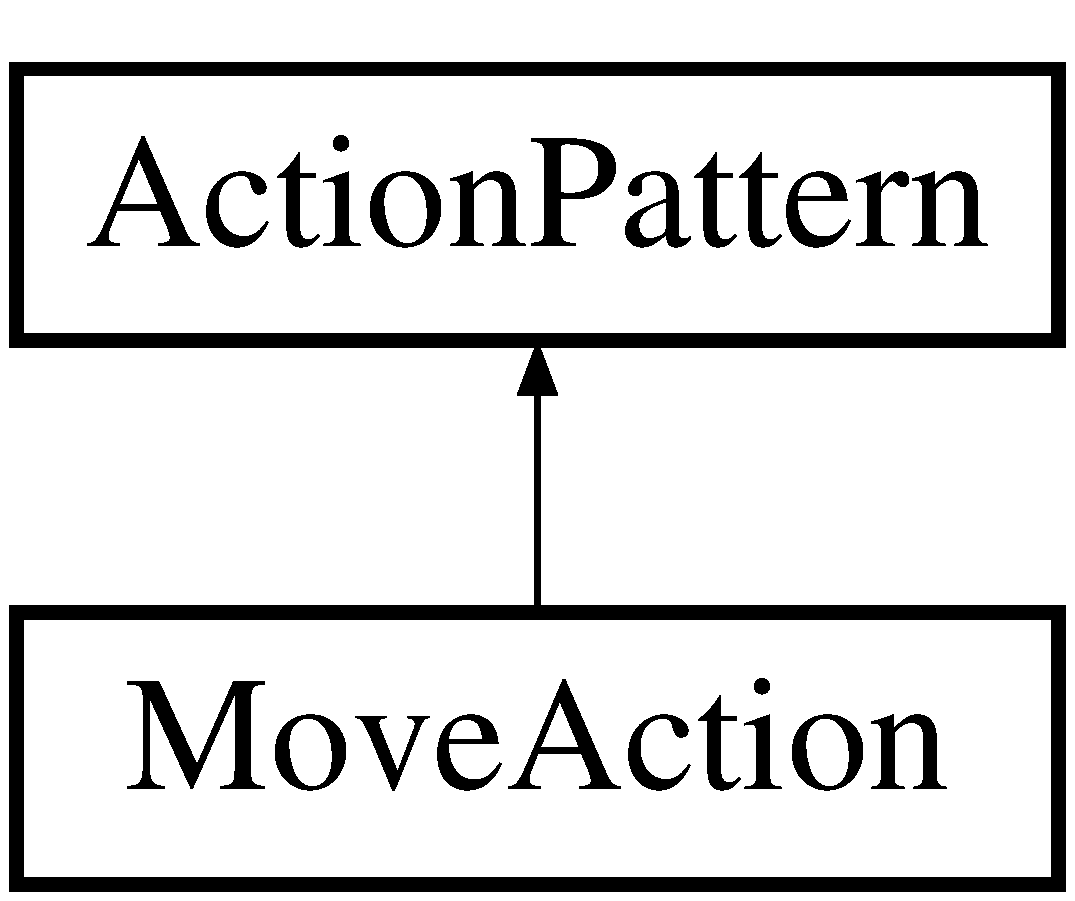
\includegraphics[height=2.000000cm]{class_move_action}
\end{center}
\end{figure}
\subsection*{公開メンバ関数}
\begin{DoxyCompactItemize}
\item 
void \mbox{\hyperlink{class_move_action_a0861a4a0fcbab38f8c33ed02b9f3c1b8}{Init}} () final
\item 
std\+::shared\+\_\+ptr$<$ \mbox{\hyperlink{class_action_pattern}{Action\+Pattern}} $>$ \mbox{\hyperlink{class_move_action_aa731fa679786c8c61965dfcd258c6c66}{Action}} (std\+::shared\+\_\+ptr$<$ \mbox{\hyperlink{class_action_pattern}{Action\+Pattern}} $>$ \&, \mbox{\hyperlink{class_boss}{Boss}} \&, const float) final
\item 
void \mbox{\hyperlink{class_move_action_a3f427440c2409e0633ff0f6040a0320c}{Render}} () final
\item 
void \mbox{\hyperlink{class_move_action_a48727a426f2a69ed62631af8385ff6ef}{Destroy}} () final
\end{DoxyCompactItemize}


\subsection{関数詳解}
\mbox{\Hypertarget{class_move_action_aa731fa679786c8c61965dfcd258c6c66}\label{class_move_action_aa731fa679786c8c61965dfcd258c6c66}} 
\index{Move\+Action@{Move\+Action}!Action@{Action}}
\index{Action@{Action}!Move\+Action@{Move\+Action}}
\subsubsection{\texorpdfstring{Action()}{Action()}}
{\footnotesize\ttfamily std\+::shared\+\_\+ptr$<$ \mbox{\hyperlink{class_action_pattern}{Action\+Pattern}} $>$ Move\+Action\+::\+Action (\begin{DoxyParamCaption}\item[{std\+::shared\+\_\+ptr$<$ \mbox{\hyperlink{class_action_pattern}{Action\+Pattern}} $>$ \&}]{action\+\_\+ptr,  }\item[{\mbox{\hyperlink{class_boss}{Boss}} \&}]{boss,  }\item[{const float}]{ }\end{DoxyParamCaption})\hspace{0.3cm}{\ttfamily [final]}, {\ttfamily [virtual]}}



\mbox{\hyperlink{class_action_pattern_a04c8daf0bf5e263303f7d86aec20eb27}{Action\+Pattern}}を実装しています。

\mbox{\Hypertarget{class_move_action_a48727a426f2a69ed62631af8385ff6ef}\label{class_move_action_a48727a426f2a69ed62631af8385ff6ef}} 
\index{Move\+Action@{Move\+Action}!Destroy@{Destroy}}
\index{Destroy@{Destroy}!Move\+Action@{Move\+Action}}
\subsubsection{\texorpdfstring{Destroy()}{Destroy()}}
{\footnotesize\ttfamily void Move\+Action\+::\+Destroy (\begin{DoxyParamCaption}{ }\end{DoxyParamCaption})\hspace{0.3cm}{\ttfamily [final]}, {\ttfamily [virtual]}}



\mbox{\hyperlink{class_action_pattern_a73833df08867c4f4785ddf51344eca47}{Action\+Pattern}}を実装しています。

\mbox{\Hypertarget{class_move_action_a0861a4a0fcbab38f8c33ed02b9f3c1b8}\label{class_move_action_a0861a4a0fcbab38f8c33ed02b9f3c1b8}} 
\index{Move\+Action@{Move\+Action}!Init@{Init}}
\index{Init@{Init}!Move\+Action@{Move\+Action}}
\subsubsection{\texorpdfstring{Init()}{Init()}}
{\footnotesize\ttfamily void Move\+Action\+::\+Init (\begin{DoxyParamCaption}{ }\end{DoxyParamCaption})\hspace{0.3cm}{\ttfamily [final]}, {\ttfamily [virtual]}}



\mbox{\hyperlink{class_action_pattern_ac8f2228ca469ce6fe29a9775bf393e0e}{Action\+Pattern}}を実装しています。

\mbox{\Hypertarget{class_move_action_a3f427440c2409e0633ff0f6040a0320c}\label{class_move_action_a3f427440c2409e0633ff0f6040a0320c}} 
\index{Move\+Action@{Move\+Action}!Render@{Render}}
\index{Render@{Render}!Move\+Action@{Move\+Action}}
\subsubsection{\texorpdfstring{Render()}{Render()}}
{\footnotesize\ttfamily void Move\+Action\+::\+Render (\begin{DoxyParamCaption}{ }\end{DoxyParamCaption})\hspace{0.3cm}{\ttfamily [final]}, {\ttfamily [virtual]}}



\mbox{\hyperlink{class_action_pattern_a313199aa5d15b6f9381b916ffe23fe6a}{Action\+Pattern}}を実装しています。



このクラス詳解は次のファイルから抽出されました\+:\begin{DoxyCompactItemize}
\item 
C\+:/\+Users/tokir/\+Documents/\+Git\+Hub/\+Weapon\+Merchant\+Adventure/src/src/object/character/enemy/boss/action\+\_\+pattern/move/\mbox{\hyperlink{move__action_8h}{move\+\_\+action.\+h}}\item 
C\+:/\+Users/tokir/\+Documents/\+Git\+Hub/\+Weapon\+Merchant\+Adventure/src/src/object/character/enemy/boss/action\+\_\+pattern/move/\mbox{\hyperlink{move__action_8cpp}{move\+\_\+action.\+cpp}}\end{DoxyCompactItemize}

\hypertarget{structsaki_1_1multiplication}{}\section{saki\+:\+:multiplication 構造体}
\label{structsaki_1_1multiplication}\index{saki\+::multiplication@{saki\+::multiplication}}


掛け算のconstexpr対応した関数オブジェクト  




{\ttfamily \#include $<$multiplication.\+h$>$}

\subsection*{公開メンバ関数}
\begin{DoxyCompactItemize}
\item 
{\footnotesize template$<$typename T1 , typename T2 $>$ }\\constexpr auto \mbox{\hyperlink{structsaki_1_1multiplication_ad7c9cfc08911b6db3ea95d4cfd5ffa7f}{operator()}} (const T1 \&t1, const T2 \&t2) const
\end{DoxyCompactItemize}


\subsection{詳解}
掛け算のconstexpr対応した関数オブジェクト 

\subsection{関数詳解}
\mbox{\Hypertarget{structsaki_1_1multiplication_ad7c9cfc08911b6db3ea95d4cfd5ffa7f}\label{structsaki_1_1multiplication_ad7c9cfc08911b6db3ea95d4cfd5ffa7f}} 
\index{saki\+::multiplication@{saki\+::multiplication}!operator()@{operator()}}
\index{operator()@{operator()}!saki\+::multiplication@{saki\+::multiplication}}
\subsubsection{\texorpdfstring{operator()()}{operator()()}}
{\footnotesize\ttfamily template$<$typename T1 , typename T2 $>$ \\
constexpr auto saki\+::multiplication\+::operator() (\begin{DoxyParamCaption}\item[{const T1 \&}]{t1,  }\item[{const T2 \&}]{t2 }\end{DoxyParamCaption}) const\hspace{0.3cm}{\ttfamily [inline]}}



この構造体詳解は次のファイルから抽出されました\+:\begin{DoxyCompactItemize}
\item 
C\+:/\+Users/tokir/\+Documents/\+Git\+Hub/\+Weapon\+Merchant\+Adventure/src/lib/saki/binary\+\_\+operator/\mbox{\hyperlink{multiplication_8h}{multiplication.\+h}}\end{DoxyCompactItemize}

\hypertarget{classsaki_1_1_node}{}\section{saki\+:\+:Node$<$ T $>$ クラステンプレート}
\label{classsaki_1_1_node}\index{saki\+::\+Node$<$ T $>$@{saki\+::\+Node$<$ T $>$}}


{\ttfamily \#include $<$node.\+h$>$}

saki\+:\+:Node$<$ T $>$ の継承関係図\begin{figure}[H]
\begin{center}
\leavevmode
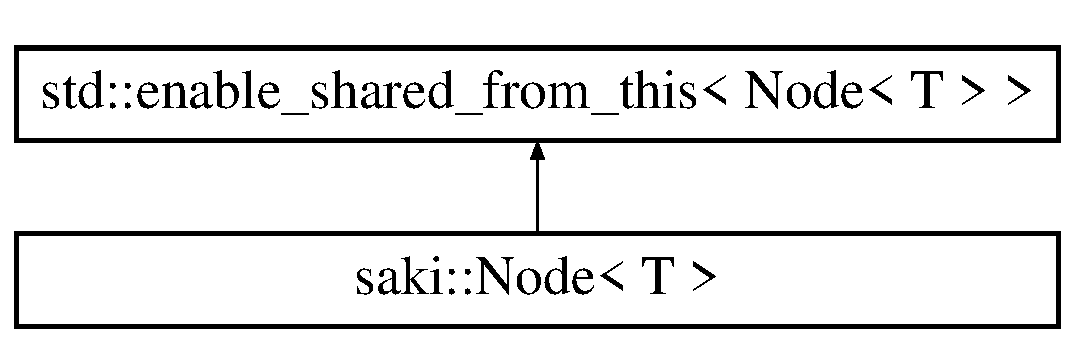
\includegraphics[height=2.000000cm]{classsaki_1_1_node}
\end{center}
\end{figure}
\subsection*{公開メンバ関数}
\begin{DoxyCompactItemize}
\item 
std\+::string \mbox{\hyperlink{classsaki_1_1_node_ab0daef362cc404496f170b3ef0a355f0}{get\+\_\+name}} () const
\begin{DoxyCompactList}\small\item\em ノード名の取得 \end{DoxyCompactList}\item 
std\+::string \mbox{\hyperlink{classsaki_1_1_node_a5aa0d398aa417048879bc71d51ce2aa3}{get\+\_\+path}} () const
\begin{DoxyCompactList}\small\item\em パスの取得 \end{DoxyCompactList}\item 
int \mbox{\hyperlink{classsaki_1_1_node_a8351b7ef227bc1f97f4d82748d6aa2a3}{get\+\_\+depth}} () const
\begin{DoxyCompactList}\small\item\em 深度の取得 \end{DoxyCompactList}\item 
std\+::shared\+\_\+ptr$<$ \mbox{\hyperlink{classsaki_1_1_node}{Node}}$<$ T $>$ $>$ \mbox{\hyperlink{classsaki_1_1_node_acc2ba97cc286656b167548214c459243}{add\+\_\+child}} (const std\+::string \&node\+\_\+name, T t)
\begin{DoxyCompactList}\small\item\em 子の追加 \end{DoxyCompactList}\item 
\mbox{\hyperlink{classsaki_1_1_node_a181585031c9062f15fba568b709a8cde}{Node}} (std\+::shared\+\_\+ptr$<$ \mbox{\hyperlink{classsaki_1_1_node}{Node}}$<$ T $>$$>$ \&p\+\_\+ptr, const std\+::string \&node\+\_\+name, const std\+::string \&current\+\_\+path, const int \+\_\+depth, T t)
\begin{DoxyCompactList}\small\item\em コンストラクタと同時に親とノード名を決定する \end{DoxyCompactList}\item 
\mbox{\hyperlink{classsaki_1_1_node_a100d4e1cfc9f04e51f405ee1d41d654b}{Node}} (std\+::shared\+\_\+ptr$<$ \mbox{\hyperlink{classsaki_1_1_node}{Node}}$<$ T $>$$>$ \&p\+\_\+ptr, const std\+::string \&node\+\_\+name, T t)
\begin{DoxyCompactList}\small\item\em コンストラクタ(ルート限定) \end{DoxyCompactList}\item 
std\+::shared\+\_\+ptr$<$ \mbox{\hyperlink{classsaki_1_1_node}{Node}}$<$ T $>$ $>$ \mbox{\hyperlink{classsaki_1_1_node_aa94a7a9a0de9e7d6c5cc362493edc5f5}{get\+\_\+node}} (const std\+::string \&node\+\_\+path=\char`\"{}\char`\"{}) const
\begin{DoxyCompactList}\small\item\em 自分自身をカレントディレクトリとしてノードをめぐり、たどり着いたノードを返す \end{DoxyCompactList}\item 
void \mbox{\hyperlink{classsaki_1_1_node_a57d63d7ba5c2f3bba02a042bbad12dc4}{delete\+\_\+node}} ()
\begin{DoxyCompactList}\small\item\em ノードの削除 \end{DoxyCompactList}\item 
{\footnotesize template$<$typename Func , typename ... T$>$ }\\void \mbox{\hyperlink{classsaki_1_1_node_aad51acc43e01039b19d22f4f09689f3b}{all\+\_\+child\+\_\+func}} (Func \&\&func, T ...t)
\begin{DoxyCompactList}\small\item\em 自分自身と自分以下の子ノードすべてに関数を実行する \end{DoxyCompactList}\item 
T \mbox{\hyperlink{classsaki_1_1_node_a9e88537adb4d8b79fe456f2496ed1bca}{get\+\_\+value}} () const
\begin{DoxyCompactList}\small\item\em 値の取得 \end{DoxyCompactList}\item 
T \& \mbox{\hyperlink{classsaki_1_1_node_a91d632d4db82e0415f394b14c5f6ce58}{get\+\_\+reference}} () const
\begin{DoxyCompactList}\small\item\em 値の参照の取得 \end{DoxyCompactList}\item 
void \mbox{\hyperlink{classsaki_1_1_node_a0ea2c2df4ce2032a5c07e955df4b0046}{copy\+\_\+node}} (const std\+::shared\+\_\+ptr$<$ \mbox{\hyperlink{classsaki_1_1_node}{Node}}$<$ T $>$$>$ \&other\+\_\+node)
\begin{DoxyCompactList}\small\item\em ノードのコピー \end{DoxyCompactList}\item 
void \mbox{\hyperlink{classsaki_1_1_node_ad6fc40d14da87ba8cb39e21bb8f16cdc}{move\+\_\+node}} (std\+::shared\+\_\+ptr$<$ \mbox{\hyperlink{classsaki_1_1_node}{Node}}$<$ T $>$$>$ \&\&other\+\_\+node) noexcept
\begin{DoxyCompactList}\small\item\em ノードのムーブ \end{DoxyCompactList}\item 
void \mbox{\hyperlink{classsaki_1_1_node_ac5b08cdb3fd3c60e38d849b7d18a9782}{node\+\_\+print}} ()
\begin{DoxyCompactList}\small\item\em デバッグ用の出力関数 \end{DoxyCompactList}\end{DoxyCompactItemize}
\subsection*{フレンド}
\begin{DoxyCompactItemize}
\item 
class \mbox{\hyperlink{classsaki_1_1_node_a151ca71f2c751d8a163f3f99ccf6cec9}{Tree$<$ T $>$}}
\end{DoxyCompactItemize}


\subsection{構築子と解体子}
\mbox{\Hypertarget{classsaki_1_1_node_a181585031c9062f15fba568b709a8cde}\label{classsaki_1_1_node_a181585031c9062f15fba568b709a8cde}} 
\index{saki\+::\+Node@{saki\+::\+Node}!Node@{Node}}
\index{Node@{Node}!saki\+::\+Node@{saki\+::\+Node}}
\subsubsection{\texorpdfstring{Node()}{Node()}\hspace{0.1cm}{\footnotesize\ttfamily [1/2]}}
{\footnotesize\ttfamily template$<$typename T $>$ \\
\mbox{\hyperlink{classsaki_1_1_node}{saki\+::\+Node}}$<$ T $>$\+::\mbox{\hyperlink{classsaki_1_1_node}{Node}} (\begin{DoxyParamCaption}\item[{std\+::shared\+\_\+ptr$<$ \mbox{\hyperlink{classsaki_1_1_node}{Node}}$<$ T $>$$>$ \&}]{p\+\_\+ptr,  }\item[{const std\+::string \&}]{node\+\_\+name,  }\item[{const std\+::string \&}]{current\+\_\+path,  }\item[{const int}]{\+\_\+depth,  }\item[{T}]{t }\end{DoxyParamCaption})\hspace{0.3cm}{\ttfamily [inline]}}



コンストラクタと同時に親とノード名を決定する 


\begin{DoxyParams}{引数}
{\em p\+\_\+ptr} & 親 \\
\hline
{\em node\+\_\+name} & ノード名 \\
\hline
{\em current\+\_\+path} & 現在のパス \\
\hline
{\em \+\_\+depth} & 親ノードの深さ \\
\hline
{\em t} & 初期値 \\
\hline
\end{DoxyParams}
\mbox{\Hypertarget{classsaki_1_1_node_a100d4e1cfc9f04e51f405ee1d41d654b}\label{classsaki_1_1_node_a100d4e1cfc9f04e51f405ee1d41d654b}} 
\index{saki\+::\+Node@{saki\+::\+Node}!Node@{Node}}
\index{Node@{Node}!saki\+::\+Node@{saki\+::\+Node}}
\subsubsection{\texorpdfstring{Node()}{Node()}\hspace{0.1cm}{\footnotesize\ttfamily [2/2]}}
{\footnotesize\ttfamily template$<$typename T $>$ \\
\mbox{\hyperlink{classsaki_1_1_node}{saki\+::\+Node}}$<$ T $>$\+::\mbox{\hyperlink{classsaki_1_1_node}{Node}} (\begin{DoxyParamCaption}\item[{std\+::shared\+\_\+ptr$<$ \mbox{\hyperlink{classsaki_1_1_node}{Node}}$<$ T $>$$>$ \&}]{p\+\_\+ptr,  }\item[{const std\+::string \&}]{node\+\_\+name,  }\item[{T}]{t }\end{DoxyParamCaption})\hspace{0.3cm}{\ttfamily [inline]}}



コンストラクタ(ルート限定) 


\begin{DoxyParams}{引数}
{\em p\+\_\+ptr} & 親 \\
\hline
{\em node\+\_\+name} & ノード名 \\
\hline
{\em t} & 初期値 \\
\hline
\end{DoxyParams}


\subsection{関数詳解}
\mbox{\Hypertarget{classsaki_1_1_node_acc2ba97cc286656b167548214c459243}\label{classsaki_1_1_node_acc2ba97cc286656b167548214c459243}} 
\index{saki\+::\+Node@{saki\+::\+Node}!add\+\_\+child@{add\+\_\+child}}
\index{add\+\_\+child@{add\+\_\+child}!saki\+::\+Node@{saki\+::\+Node}}
\subsubsection{\texorpdfstring{add\+\_\+child()}{add\_child()}}
{\footnotesize\ttfamily template$<$typename T $>$ \\
std\+::shared\+\_\+ptr$<$\mbox{\hyperlink{classsaki_1_1_node}{Node}}$<$T$>$ $>$ \mbox{\hyperlink{classsaki_1_1_node}{saki\+::\+Node}}$<$ T $>$\+::add\+\_\+child (\begin{DoxyParamCaption}\item[{const std\+::string \&}]{node\+\_\+name,  }\item[{T}]{t }\end{DoxyParamCaption})\hspace{0.3cm}{\ttfamily [inline]}}



子の追加 


\begin{DoxyParams}{引数}
{\em c\+\_\+itr} & 子 \\
\hline
{\em t} & 初期値 \\
\hline
\end{DoxyParams}
\mbox{\Hypertarget{classsaki_1_1_node_aad51acc43e01039b19d22f4f09689f3b}\label{classsaki_1_1_node_aad51acc43e01039b19d22f4f09689f3b}} 
\index{saki\+::\+Node@{saki\+::\+Node}!all\+\_\+child\+\_\+func@{all\+\_\+child\+\_\+func}}
\index{all\+\_\+child\+\_\+func@{all\+\_\+child\+\_\+func}!saki\+::\+Node@{saki\+::\+Node}}
\subsubsection{\texorpdfstring{all\+\_\+child\+\_\+func()}{all\_child\_func()}}
{\footnotesize\ttfamily template$<$typename T $>$ \\
template$<$typename Func , typename ... T$>$ \\
void \mbox{\hyperlink{classsaki_1_1_node}{saki\+::\+Node}}$<$ T $>$\+::all\+\_\+child\+\_\+func (\begin{DoxyParamCaption}\item[{Func \&\&}]{func,  }\item[{T ...}]{t }\end{DoxyParamCaption})\hspace{0.3cm}{\ttfamily [inline]}}



自分自身と自分以下の子ノードすべてに関数を実行する 


\begin{DoxyParams}{引数}
{\em func} & 関数 \\
\hline
{\em t} & 第二引数以降の引数 \\
\hline
\end{DoxyParams}
\mbox{\Hypertarget{classsaki_1_1_node_a0ea2c2df4ce2032a5c07e955df4b0046}\label{classsaki_1_1_node_a0ea2c2df4ce2032a5c07e955df4b0046}} 
\index{saki\+::\+Node@{saki\+::\+Node}!copy\+\_\+node@{copy\+\_\+node}}
\index{copy\+\_\+node@{copy\+\_\+node}!saki\+::\+Node@{saki\+::\+Node}}
\subsubsection{\texorpdfstring{copy\+\_\+node()}{copy\_node()}}
{\footnotesize\ttfamily template$<$typename T $>$ \\
void \mbox{\hyperlink{classsaki_1_1_node}{saki\+::\+Node}}$<$ T $>$\+::copy\+\_\+node (\begin{DoxyParamCaption}\item[{const std\+::shared\+\_\+ptr$<$ \mbox{\hyperlink{classsaki_1_1_node}{Node}}$<$ T $>$$>$ \&}]{other\+\_\+node }\end{DoxyParamCaption})\hspace{0.3cm}{\ttfamily [inline]}}



ノードのコピー 


\begin{DoxyParams}{引数}
{\em other\+\_\+node} & コピーするノード \\
\hline
\end{DoxyParams}
\mbox{\Hypertarget{classsaki_1_1_node_a57d63d7ba5c2f3bba02a042bbad12dc4}\label{classsaki_1_1_node_a57d63d7ba5c2f3bba02a042bbad12dc4}} 
\index{saki\+::\+Node@{saki\+::\+Node}!delete\+\_\+node@{delete\+\_\+node}}
\index{delete\+\_\+node@{delete\+\_\+node}!saki\+::\+Node@{saki\+::\+Node}}
\subsubsection{\texorpdfstring{delete\+\_\+node()}{delete\_node()}}
{\footnotesize\ttfamily template$<$typename T $>$ \\
void \mbox{\hyperlink{classsaki_1_1_node}{saki\+::\+Node}}$<$ T $>$\+::delete\+\_\+node (\begin{DoxyParamCaption}{ }\end{DoxyParamCaption})\hspace{0.3cm}{\ttfamily [inline]}}



ノードの削除 

\mbox{\Hypertarget{classsaki_1_1_node_a8351b7ef227bc1f97f4d82748d6aa2a3}\label{classsaki_1_1_node_a8351b7ef227bc1f97f4d82748d6aa2a3}} 
\index{saki\+::\+Node@{saki\+::\+Node}!get\+\_\+depth@{get\+\_\+depth}}
\index{get\+\_\+depth@{get\+\_\+depth}!saki\+::\+Node@{saki\+::\+Node}}
\subsubsection{\texorpdfstring{get\+\_\+depth()}{get\_depth()}}
{\footnotesize\ttfamily template$<$typename T $>$ \\
int \mbox{\hyperlink{classsaki_1_1_node}{saki\+::\+Node}}$<$ T $>$\+::get\+\_\+depth (\begin{DoxyParamCaption}{ }\end{DoxyParamCaption}) const\hspace{0.3cm}{\ttfamily [inline]}}



深度の取得 

\begin{DoxyReturn}{戻り値}
深度 
\end{DoxyReturn}
\mbox{\Hypertarget{classsaki_1_1_node_ab0daef362cc404496f170b3ef0a355f0}\label{classsaki_1_1_node_ab0daef362cc404496f170b3ef0a355f0}} 
\index{saki\+::\+Node@{saki\+::\+Node}!get\+\_\+name@{get\+\_\+name}}
\index{get\+\_\+name@{get\+\_\+name}!saki\+::\+Node@{saki\+::\+Node}}
\subsubsection{\texorpdfstring{get\+\_\+name()}{get\_name()}}
{\footnotesize\ttfamily template$<$typename T $>$ \\
std\+::string \mbox{\hyperlink{classsaki_1_1_node}{saki\+::\+Node}}$<$ T $>$\+::get\+\_\+name (\begin{DoxyParamCaption}{ }\end{DoxyParamCaption}) const\hspace{0.3cm}{\ttfamily [inline]}}



ノード名の取得 

\begin{DoxyReturn}{戻り値}
ノード名 
\end{DoxyReturn}
\mbox{\Hypertarget{classsaki_1_1_node_aa94a7a9a0de9e7d6c5cc362493edc5f5}\label{classsaki_1_1_node_aa94a7a9a0de9e7d6c5cc362493edc5f5}} 
\index{saki\+::\+Node@{saki\+::\+Node}!get\+\_\+node@{get\+\_\+node}}
\index{get\+\_\+node@{get\+\_\+node}!saki\+::\+Node@{saki\+::\+Node}}
\subsubsection{\texorpdfstring{get\+\_\+node()}{get\_node()}}
{\footnotesize\ttfamily template$<$typename T $>$ \\
std\+::shared\+\_\+ptr$<$\mbox{\hyperlink{classsaki_1_1_node}{Node}}$<$T$>$ $>$ \mbox{\hyperlink{classsaki_1_1_node}{saki\+::\+Node}}$<$ T $>$\+::get\+\_\+node (\begin{DoxyParamCaption}\item[{const std\+::string \&}]{node\+\_\+path = {\ttfamily \char`\"{}\char`\"{}} }\end{DoxyParamCaption}) const\hspace{0.3cm}{\ttfamily [inline]}}



自分自身をカレントディレクトリとしてノードをめぐり、たどり着いたノードを返す 

失敗すると自分自身を返す \mbox{\Hypertarget{classsaki_1_1_node_a5aa0d398aa417048879bc71d51ce2aa3}\label{classsaki_1_1_node_a5aa0d398aa417048879bc71d51ce2aa3}} 
\index{saki\+::\+Node@{saki\+::\+Node}!get\+\_\+path@{get\+\_\+path}}
\index{get\+\_\+path@{get\+\_\+path}!saki\+::\+Node@{saki\+::\+Node}}
\subsubsection{\texorpdfstring{get\+\_\+path()}{get\_path()}}
{\footnotesize\ttfamily template$<$typename T $>$ \\
std\+::string \mbox{\hyperlink{classsaki_1_1_node}{saki\+::\+Node}}$<$ T $>$\+::get\+\_\+path (\begin{DoxyParamCaption}{ }\end{DoxyParamCaption}) const\hspace{0.3cm}{\ttfamily [inline]}}



パスの取得 

\begin{DoxyReturn}{戻り値}
パス 
\end{DoxyReturn}
\mbox{\Hypertarget{classsaki_1_1_node_a91d632d4db82e0415f394b14c5f6ce58}\label{classsaki_1_1_node_a91d632d4db82e0415f394b14c5f6ce58}} 
\index{saki\+::\+Node@{saki\+::\+Node}!get\+\_\+reference@{get\+\_\+reference}}
\index{get\+\_\+reference@{get\+\_\+reference}!saki\+::\+Node@{saki\+::\+Node}}
\subsubsection{\texorpdfstring{get\+\_\+reference()}{get\_reference()}}
{\footnotesize\ttfamily template$<$typename T $>$ \\
T\& \mbox{\hyperlink{classsaki_1_1_node}{saki\+::\+Node}}$<$ T $>$\+::get\+\_\+reference (\begin{DoxyParamCaption}{ }\end{DoxyParamCaption}) const\hspace{0.3cm}{\ttfamily [inline]}}



値の参照の取得 

\begin{DoxyReturn}{戻り値}
値の参照 
\end{DoxyReturn}
\mbox{\Hypertarget{classsaki_1_1_node_a9e88537adb4d8b79fe456f2496ed1bca}\label{classsaki_1_1_node_a9e88537adb4d8b79fe456f2496ed1bca}} 
\index{saki\+::\+Node@{saki\+::\+Node}!get\+\_\+value@{get\+\_\+value}}
\index{get\+\_\+value@{get\+\_\+value}!saki\+::\+Node@{saki\+::\+Node}}
\subsubsection{\texorpdfstring{get\+\_\+value()}{get\_value()}}
{\footnotesize\ttfamily template$<$typename T $>$ \\
T \mbox{\hyperlink{classsaki_1_1_node}{saki\+::\+Node}}$<$ T $>$\+::get\+\_\+value (\begin{DoxyParamCaption}{ }\end{DoxyParamCaption}) const\hspace{0.3cm}{\ttfamily [inline]}}



値の取得 

\begin{DoxyReturn}{戻り値}
値 
\end{DoxyReturn}
\mbox{\Hypertarget{classsaki_1_1_node_ad6fc40d14da87ba8cb39e21bb8f16cdc}\label{classsaki_1_1_node_ad6fc40d14da87ba8cb39e21bb8f16cdc}} 
\index{saki\+::\+Node@{saki\+::\+Node}!move\+\_\+node@{move\+\_\+node}}
\index{move\+\_\+node@{move\+\_\+node}!saki\+::\+Node@{saki\+::\+Node}}
\subsubsection{\texorpdfstring{move\+\_\+node()}{move\_node()}}
{\footnotesize\ttfamily template$<$typename T $>$ \\
void \mbox{\hyperlink{classsaki_1_1_node}{saki\+::\+Node}}$<$ T $>$\+::move\+\_\+node (\begin{DoxyParamCaption}\item[{std\+::shared\+\_\+ptr$<$ \mbox{\hyperlink{classsaki_1_1_node}{Node}}$<$ T $>$$>$ \&\&}]{other\+\_\+node }\end{DoxyParamCaption})\hspace{0.3cm}{\ttfamily [inline]}, {\ttfamily [noexcept]}}



ノードのムーブ 


\begin{DoxyParams}{引数}
{\em other\+\_\+node} & ムーブするノード \\
\hline
\end{DoxyParams}
\mbox{\Hypertarget{classsaki_1_1_node_ac5b08cdb3fd3c60e38d849b7d18a9782}\label{classsaki_1_1_node_ac5b08cdb3fd3c60e38d849b7d18a9782}} 
\index{saki\+::\+Node@{saki\+::\+Node}!node\+\_\+print@{node\+\_\+print}}
\index{node\+\_\+print@{node\+\_\+print}!saki\+::\+Node@{saki\+::\+Node}}
\subsubsection{\texorpdfstring{node\+\_\+print()}{node\_print()}}
{\footnotesize\ttfamily template$<$typename T $>$ \\
void \mbox{\hyperlink{classsaki_1_1_node}{saki\+::\+Node}}$<$ T $>$\+::node\+\_\+print (\begin{DoxyParamCaption}{ }\end{DoxyParamCaption})\hspace{0.3cm}{\ttfamily [inline]}}



デバッグ用の出力関数 



\subsection{フレンドと関連関数の詳解}
\mbox{\Hypertarget{classsaki_1_1_node_a151ca71f2c751d8a163f3f99ccf6cec9}\label{classsaki_1_1_node_a151ca71f2c751d8a163f3f99ccf6cec9}} 
\index{saki\+::\+Node@{saki\+::\+Node}!Tree$<$ T $>$@{Tree$<$ T $>$}}
\index{Tree$<$ T $>$@{Tree$<$ T $>$}!saki\+::\+Node@{saki\+::\+Node}}
\subsubsection{\texorpdfstring{Tree$<$ T $>$}{Tree< T >}}
{\footnotesize\ttfamily template$<$typename T $>$ \\
friend class \mbox{\hyperlink{classsaki_1_1_tree}{Tree}}$<$ T $>$\hspace{0.3cm}{\ttfamily [friend]}}



このクラス詳解は次のファイルから抽出されました\+:\begin{DoxyCompactItemize}
\item 
C\+:/\+Users/tokir/\+Documents/\+Git\+Hub/\+Weapon\+Merchant\+Adventure/src/lib/saki/tree/node/\mbox{\hyperlink{node_8h}{node.\+h}}\end{DoxyCompactItemize}

\hypertarget{class_normal_enemy}{}\section{Normal\+Enemy クラス}
\label{class_normal_enemy}\index{Normal\+Enemy@{Normal\+Enemy}}


ノーマルな敵クラス  




{\ttfamily \#include $<$normal\+\_\+enemy.\+h$>$}

Normal\+Enemy の継承関係図\begin{figure}[H]
\begin{center}
\leavevmode
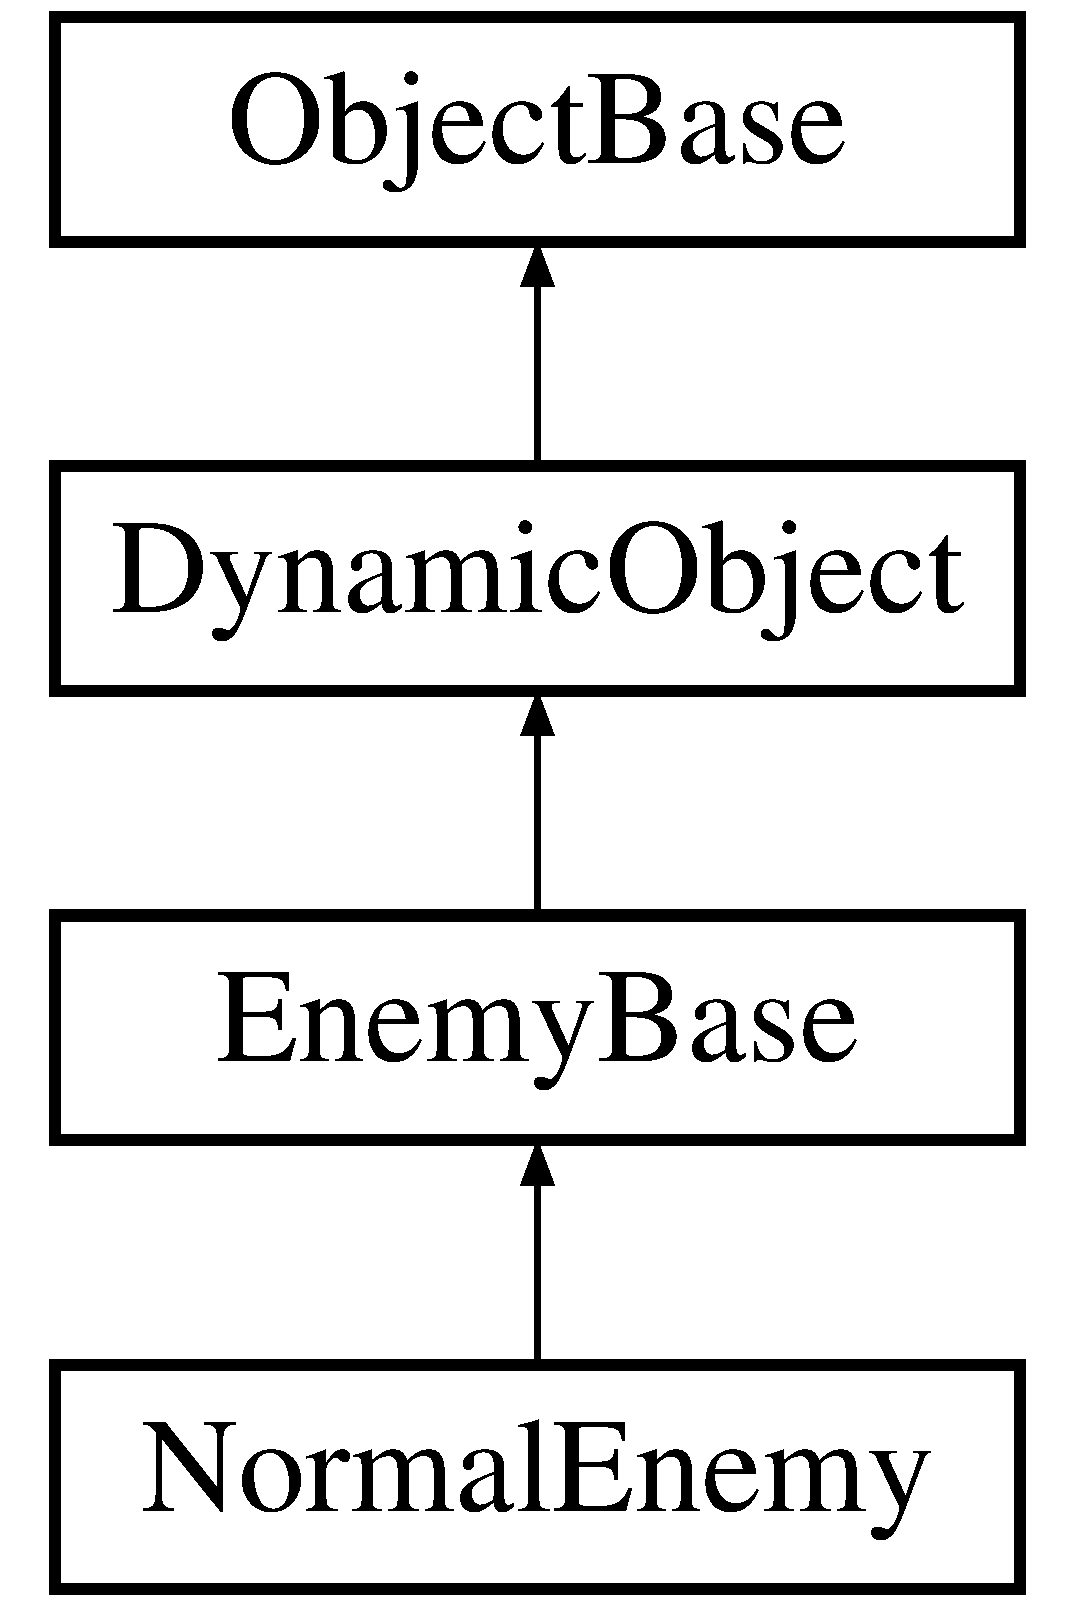
\includegraphics[height=4.000000cm]{class_normal_enemy}
\end{center}
\end{figure}
\subsection*{公開メンバ関数}
\begin{DoxyCompactItemize}
\item 
\mbox{\hyperlink{class_normal_enemy_aa386eea59a2983574fe7d55a91f93012}{Normal\+Enemy}} ()
\begin{DoxyCompactList}\small\item\em コンストラクタ \end{DoxyCompactList}\item 
\mbox{\hyperlink{class_normal_enemy_a08bfcea97297d0cff5c10854c8f5ffb8}{Normal\+Enemy}} (const \mbox{\hyperlink{class_normal_enemy}{Normal\+Enemy}} \&ne)
\begin{DoxyCompactList}\small\item\em コピーコンストラクタ \end{DoxyCompactList}\item 
\mbox{\hyperlink{class_normal_enemy_a64edfeecedfae67d33a5e1fcdccbbfa6}{Normal\+Enemy}} (\mbox{\hyperlink{class_normal_enemy}{Normal\+Enemy}} \&\&ne) noexcept
\begin{DoxyCompactList}\small\item\em ムーブコンストラクタ \end{DoxyCompactList}\item 
\mbox{\hyperlink{class_normal_enemy}{Normal\+Enemy}} \& \mbox{\hyperlink{class_normal_enemy_a4294020d85d9ae77a47294e04fd048b6}{operator=}} (const \mbox{\hyperlink{class_normal_enemy}{Normal\+Enemy}} \&other)
\begin{DoxyCompactList}\small\item\em コピー代入演算子 \end{DoxyCompactList}\item 
void \mbox{\hyperlink{class_normal_enemy_a71cb11fe60d713ce638dcec5d66912e6}{Collision}} (\mbox{\hyperlink{class_object_base}{Object\+Base}} $\ast$, \mbox{\hyperlink{common_8h_ae148fff5818e9444b4ab2288829559bf}{Vec2}}) final
\begin{DoxyCompactList}\small\item\em エネミーの当たったときに実行する関数 \end{DoxyCompactList}\item 
void \mbox{\hyperlink{class_normal_enemy_a8a4271b6da6c7679d134d1c08125815b}{Destroy}} () final
\begin{DoxyCompactList}\small\item\em エネミーの破棄 \end{DoxyCompactList}\item 
void \mbox{\hyperlink{class_normal_enemy_a9fe91caeeb6d9882e108c8c0d9d404c1}{Change\+Dire}} ()
\item 
\mbox{\hyperlink{class_normal_enemy_adc9a3115b2494739261b5cc363c11c32}{$\sim$\+Normal\+Enemy}} ()
\begin{DoxyCompactList}\small\item\em デストラクタ \end{DoxyCompactList}\end{DoxyCompactItemize}
\subsection*{限定公開メンバ関数}
\begin{DoxyCompactItemize}
\item 
void \mbox{\hyperlink{class_normal_enemy_ae45bd9535595f810d065b92f8dd63342}{Init\+Process}} () final
\begin{DoxyCompactList}\small\item\em エネミーの初期化 \end{DoxyCompactList}\item 
void \mbox{\hyperlink{class_normal_enemy_a9f66e4bf18310ec7c5dc679bea78fa8e}{Update\+Process}} ()
\begin{DoxyCompactList}\small\item\em エネミーの更新 \end{DoxyCompactList}\end{DoxyCompactItemize}
\subsection*{その他の継承メンバ}


\subsection{詳解}
ノーマルな敵クラス 

\subsection{構築子と解体子}
\mbox{\Hypertarget{class_normal_enemy_aa386eea59a2983574fe7d55a91f93012}\label{class_normal_enemy_aa386eea59a2983574fe7d55a91f93012}} 
\index{Normal\+Enemy@{Normal\+Enemy}!Normal\+Enemy@{Normal\+Enemy}}
\index{Normal\+Enemy@{Normal\+Enemy}!Normal\+Enemy@{Normal\+Enemy}}
\subsubsection{\texorpdfstring{Normal\+Enemy()}{NormalEnemy()}\hspace{0.1cm}{\footnotesize\ttfamily [1/3]}}
{\footnotesize\ttfamily Normal\+Enemy\+::\+Normal\+Enemy (\begin{DoxyParamCaption}{ }\end{DoxyParamCaption})\hspace{0.3cm}{\ttfamily [inline]}}



コンストラクタ 

\mbox{\Hypertarget{class_normal_enemy_a08bfcea97297d0cff5c10854c8f5ffb8}\label{class_normal_enemy_a08bfcea97297d0cff5c10854c8f5ffb8}} 
\index{Normal\+Enemy@{Normal\+Enemy}!Normal\+Enemy@{Normal\+Enemy}}
\index{Normal\+Enemy@{Normal\+Enemy}!Normal\+Enemy@{Normal\+Enemy}}
\subsubsection{\texorpdfstring{Normal\+Enemy()}{NormalEnemy()}\hspace{0.1cm}{\footnotesize\ttfamily [2/3]}}
{\footnotesize\ttfamily Normal\+Enemy\+::\+Normal\+Enemy (\begin{DoxyParamCaption}\item[{const \mbox{\hyperlink{class_normal_enemy}{Normal\+Enemy}} \&}]{ne }\end{DoxyParamCaption})\hspace{0.3cm}{\ttfamily [inline]}}



コピーコンストラクタ 

\mbox{\Hypertarget{class_normal_enemy_a64edfeecedfae67d33a5e1fcdccbbfa6}\label{class_normal_enemy_a64edfeecedfae67d33a5e1fcdccbbfa6}} 
\index{Normal\+Enemy@{Normal\+Enemy}!Normal\+Enemy@{Normal\+Enemy}}
\index{Normal\+Enemy@{Normal\+Enemy}!Normal\+Enemy@{Normal\+Enemy}}
\subsubsection{\texorpdfstring{Normal\+Enemy()}{NormalEnemy()}\hspace{0.1cm}{\footnotesize\ttfamily [3/3]}}
{\footnotesize\ttfamily Normal\+Enemy\+::\+Normal\+Enemy (\begin{DoxyParamCaption}\item[{\mbox{\hyperlink{class_normal_enemy}{Normal\+Enemy}} \&\&}]{ne }\end{DoxyParamCaption})\hspace{0.3cm}{\ttfamily [inline]}, {\ttfamily [noexcept]}}



ムーブコンストラクタ 

\mbox{\Hypertarget{class_normal_enemy_adc9a3115b2494739261b5cc363c11c32}\label{class_normal_enemy_adc9a3115b2494739261b5cc363c11c32}} 
\index{Normal\+Enemy@{Normal\+Enemy}!````~Normal\+Enemy@{$\sim$\+Normal\+Enemy}}
\index{````~Normal\+Enemy@{$\sim$\+Normal\+Enemy}!Normal\+Enemy@{Normal\+Enemy}}
\subsubsection{\texorpdfstring{$\sim$\+Normal\+Enemy()}{~NormalEnemy()}}
{\footnotesize\ttfamily Normal\+Enemy\+::$\sim$\+Normal\+Enemy (\begin{DoxyParamCaption}{ }\end{DoxyParamCaption})\hspace{0.3cm}{\ttfamily [inline]}}



デストラクタ 



\subsection{関数詳解}
\mbox{\Hypertarget{class_normal_enemy_a9fe91caeeb6d9882e108c8c0d9d404c1}\label{class_normal_enemy_a9fe91caeeb6d9882e108c8c0d9d404c1}} 
\index{Normal\+Enemy@{Normal\+Enemy}!Change\+Dire@{Change\+Dire}}
\index{Change\+Dire@{Change\+Dire}!Normal\+Enemy@{Normal\+Enemy}}
\subsubsection{\texorpdfstring{Change\+Dire()}{ChangeDire()}}
{\footnotesize\ttfamily void Normal\+Enemy\+::\+Change\+Dire (\begin{DoxyParamCaption}{ }\end{DoxyParamCaption})\hspace{0.3cm}{\ttfamily [inline]}}

\mbox{\Hypertarget{class_normal_enemy_a71cb11fe60d713ce638dcec5d66912e6}\label{class_normal_enemy_a71cb11fe60d713ce638dcec5d66912e6}} 
\index{Normal\+Enemy@{Normal\+Enemy}!Collision@{Collision}}
\index{Collision@{Collision}!Normal\+Enemy@{Normal\+Enemy}}
\subsubsection{\texorpdfstring{Collision()}{Collision()}}
{\footnotesize\ttfamily void Normal\+Enemy\+::\+Collision (\begin{DoxyParamCaption}\item[{\mbox{\hyperlink{class_object_base}{Object\+Base}} $\ast$}]{obj,  }\item[{\mbox{\hyperlink{common_8h_ae148fff5818e9444b4ab2288829559bf}{Vec2}}}]{ }\end{DoxyParamCaption})\hspace{0.3cm}{\ttfamily [final]}, {\ttfamily [virtual]}}



エネミーの当たったときに実行する関数 


\begin{DoxyParams}{引数}
{\em obj 当たった相手のオブジェクト} & \\
\hline
\end{DoxyParams}


\mbox{\hyperlink{class_object_base_a3e1db79dfa119be067d816c22d09839d}{Object\+Base}}を再実装しています。

\mbox{\Hypertarget{class_normal_enemy_a8a4271b6da6c7679d134d1c08125815b}\label{class_normal_enemy_a8a4271b6da6c7679d134d1c08125815b}} 
\index{Normal\+Enemy@{Normal\+Enemy}!Destroy@{Destroy}}
\index{Destroy@{Destroy}!Normal\+Enemy@{Normal\+Enemy}}
\subsubsection{\texorpdfstring{Destroy()}{Destroy()}}
{\footnotesize\ttfamily void Normal\+Enemy\+::\+Destroy (\begin{DoxyParamCaption}{ }\end{DoxyParamCaption})\hspace{0.3cm}{\ttfamily [final]}, {\ttfamily [virtual]}}



エネミーの破棄 



\mbox{\hyperlink{class_object_base_a7fa4c548153c3af20f89673ffea809af}{Object\+Base}}を実装しています。

\mbox{\Hypertarget{class_normal_enemy_ae45bd9535595f810d065b92f8dd63342}\label{class_normal_enemy_ae45bd9535595f810d065b92f8dd63342}} 
\index{Normal\+Enemy@{Normal\+Enemy}!Init\+Process@{Init\+Process}}
\index{Init\+Process@{Init\+Process}!Normal\+Enemy@{Normal\+Enemy}}
\subsubsection{\texorpdfstring{Init\+Process()}{InitProcess()}}
{\footnotesize\ttfamily void Normal\+Enemy\+::\+Init\+Process (\begin{DoxyParamCaption}{ }\end{DoxyParamCaption})\hspace{0.3cm}{\ttfamily [final]}, {\ttfamily [protected]}, {\ttfamily [virtual]}}



エネミーの初期化 



\mbox{\hyperlink{class_object_base_af133f36f2bca1dcfd962e2cfac61ab51}{Object\+Base}}を実装しています。

\mbox{\Hypertarget{class_normal_enemy_a4294020d85d9ae77a47294e04fd048b6}\label{class_normal_enemy_a4294020d85d9ae77a47294e04fd048b6}} 
\index{Normal\+Enemy@{Normal\+Enemy}!operator=@{operator=}}
\index{operator=@{operator=}!Normal\+Enemy@{Normal\+Enemy}}
\subsubsection{\texorpdfstring{operator=()}{operator=()}}
{\footnotesize\ttfamily \mbox{\hyperlink{class_normal_enemy}{Normal\+Enemy}}\& Normal\+Enemy\+::operator= (\begin{DoxyParamCaption}\item[{const \mbox{\hyperlink{class_normal_enemy}{Normal\+Enemy}} \&}]{other }\end{DoxyParamCaption})\hspace{0.3cm}{\ttfamily [inline]}}



コピー代入演算子 

\mbox{\Hypertarget{class_normal_enemy_a9f66e4bf18310ec7c5dc679bea78fa8e}\label{class_normal_enemy_a9f66e4bf18310ec7c5dc679bea78fa8e}} 
\index{Normal\+Enemy@{Normal\+Enemy}!Update\+Process@{Update\+Process}}
\index{Update\+Process@{Update\+Process}!Normal\+Enemy@{Normal\+Enemy}}
\subsubsection{\texorpdfstring{Update\+Process()}{UpdateProcess()}}
{\footnotesize\ttfamily void Normal\+Enemy\+::\+Update\+Process (\begin{DoxyParamCaption}{ }\end{DoxyParamCaption})\hspace{0.3cm}{\ttfamily [protected]}, {\ttfamily [virtual]}}



エネミーの更新 



\mbox{\hyperlink{class_object_base_a8b5b72b363a419767efde0b0e692ea95}{Object\+Base}}を実装しています。



このクラス詳解は次のファイルから抽出されました\+:\begin{DoxyCompactItemize}
\item 
C\+:/\+Users/tokir/\+Documents/\+Git\+Hub/\+Weapon\+Merchant\+Adventure/src/src/object/character/enemy/normal/\mbox{\hyperlink{normal__enemy_8h}{normal\+\_\+enemy.\+h}}\item 
C\+:/\+Users/tokir/\+Documents/\+Git\+Hub/\+Weapon\+Merchant\+Adventure/src/src/object/character/enemy/normal/\mbox{\hyperlink{normal__enemy_8cpp}{normal\+\_\+enemy.\+cpp}}\end{DoxyCompactItemize}

\hypertarget{class_object_base}{}\section{Object\+Base クラス}
\label{class_object_base}\index{Object\+Base@{Object\+Base}}


オブジェクトのスーパークラス  




{\ttfamily \#include $<$object\+\_\+base.\+h$>$}

Object\+Base の継承関係図\begin{figure}[H]
\begin{center}
\leavevmode
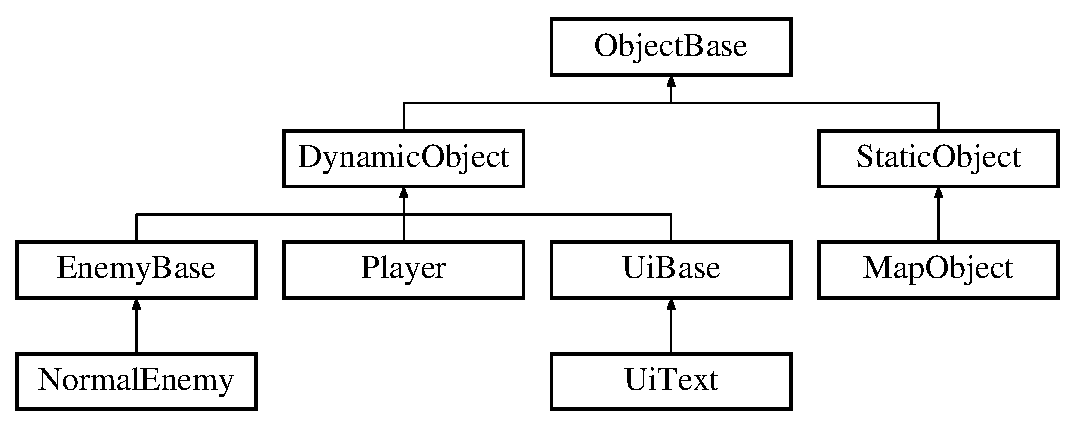
\includegraphics[height=4.000000cm]{class_object_base}
\end{center}
\end{figure}
\subsection*{公開メンバ関数}
\begin{DoxyCompactItemize}
\item 
\mbox{\hyperlink{class_object_base_af2c3a18da2d1cd1c0dd5fae168207f0c}{Object\+Base}} ()
\begin{DoxyCompactList}\small\item\em コンストラクタ \end{DoxyCompactList}\item 
void \mbox{\hyperlink{class_object_base_aea82aedc489b0a9d9990aafa06eef514}{Init}} (std\+::string name, W\+C\+H\+AR $\ast$path, const L\+O\+NG w, const L\+O\+NG h, \mbox{\hyperlink{transform_8h_afb0c5e21d4133ff4f200992c0b534e1b}{V\+E\+C2}} pos, float rot=0, float scale=1, bool all\+\_\+render=true)
\begin{DoxyCompactList}\small\item\em 初期化 \end{DoxyCompactList}\item 
void \mbox{\hyperlink{class_object_base_a5b5672034139b22235ada326eb16dd3e}{Update}} ()
\begin{DoxyCompactList}\small\item\em 更新するかどうか決める \end{DoxyCompactList}\item 
void \mbox{\hyperlink{class_object_base_ac84be5b56d23b8809ca08e27c0dcb16a}{Render}} (bool=true, const \mbox{\hyperlink{class_transform}{Transform}} \&=N\+U\+LL)
\begin{DoxyCompactList}\small\item\em 描画するかどうかを決める \end{DoxyCompactList}\item 
virtual void \mbox{\hyperlink{class_object_base_a7fa4c548153c3af20f89673ffea809af}{Destroy}} ()=0
\item 
virtual \mbox{\hyperlink{class_object_base_a7074bc9389069351c2d0eee6a47e5ee3}{$\sim$\+Object\+Base}} ()
\item 
virtual void \mbox{\hyperlink{class_object_base_a1991d1c2c214a593feb6b6b24802a8c4}{Collision}} (\mbox{\hyperlink{class_object_base}{Object\+Base}} $\ast$)
\end{DoxyCompactItemize}
\subsection*{公開変数類}
\begin{DoxyCompactItemize}
\item 
\mbox{\hyperlink{object__base_8h_a0eff9883ab049ee02773dde19d057c0c}{O\+B\+J\+E\+C\+T\+\_\+\+T\+AG}} \mbox{\hyperlink{class_object_base_aff7eb5482ca9bc1cd30b84994d0dad8b}{object\+\_\+tag}}
\item 
bool \mbox{\hyperlink{class_object_base_ade1c868f20653a6fa5236544120eca2b}{enabled}}
\item 
\mbox{\hyperlink{class_transform}{Transform}} \mbox{\hyperlink{class_object_base_ac8096c26fe09682da6119208d392dc62}{transform}}
\end{DoxyCompactItemize}
\subsection*{限定公開メンバ関数}
\begin{DoxyCompactItemize}
\item 
virtual void \mbox{\hyperlink{class_object_base_af133f36f2bca1dcfd962e2cfac61ab51}{Init\+Process}} ()=0
\item 
virtual void \mbox{\hyperlink{class_object_base_aeac51d868beeb7f7fe900407b76b93a2}{Render\+Process}} (bool)=0
\item 
virtual void \mbox{\hyperlink{class_object_base_a8b5b72b363a419767efde0b0e692ea95}{Update\+Process}} ()=0
\end{DoxyCompactItemize}
\subsection*{限定公開変数類}
\begin{DoxyCompactItemize}
\item 
\mbox{\hyperlink{class_sprite}{Sprite}} \mbox{\hyperlink{class_object_base_a16415e349623e10f45518fb637f7051b}{sprite}}
\item 
\mbox{\hyperlink{class_transform}{Transform}} \mbox{\hyperlink{class_object_base_abedc2ea4baa694611f8822ea6e04b210}{world\+Transform}}
\end{DoxyCompactItemize}


\subsection{詳解}
オブジェクトのスーパークラス 

\subsection{構築子と解体子}
\mbox{\Hypertarget{class_object_base_af2c3a18da2d1cd1c0dd5fae168207f0c}\label{class_object_base_af2c3a18da2d1cd1c0dd5fae168207f0c}} 
\index{Object\+Base@{Object\+Base}!Object\+Base@{Object\+Base}}
\index{Object\+Base@{Object\+Base}!Object\+Base@{Object\+Base}}
\subsubsection{\texorpdfstring{Object\+Base()}{ObjectBase()}}
{\footnotesize\ttfamily Object\+Base\+::\+Object\+Base (\begin{DoxyParamCaption}{ }\end{DoxyParamCaption})\hspace{0.3cm}{\ttfamily [inline]}}



コンストラクタ 

\mbox{\Hypertarget{class_object_base_a7074bc9389069351c2d0eee6a47e5ee3}\label{class_object_base_a7074bc9389069351c2d0eee6a47e5ee3}} 
\index{Object\+Base@{Object\+Base}!````~Object\+Base@{$\sim$\+Object\+Base}}
\index{````~Object\+Base@{$\sim$\+Object\+Base}!Object\+Base@{Object\+Base}}
\subsubsection{\texorpdfstring{$\sim$\+Object\+Base()}{~ObjectBase()}}
{\footnotesize\ttfamily virtual Object\+Base\+::$\sim$\+Object\+Base (\begin{DoxyParamCaption}{ }\end{DoxyParamCaption})\hspace{0.3cm}{\ttfamily [inline]}, {\ttfamily [virtual]}}



\subsection{関数詳解}
\mbox{\Hypertarget{class_object_base_a1991d1c2c214a593feb6b6b24802a8c4}\label{class_object_base_a1991d1c2c214a593feb6b6b24802a8c4}} 
\index{Object\+Base@{Object\+Base}!Collision@{Collision}}
\index{Collision@{Collision}!Object\+Base@{Object\+Base}}
\subsubsection{\texorpdfstring{Collision()}{Collision()}}
{\footnotesize\ttfamily virtual void Object\+Base\+::\+Collision (\begin{DoxyParamCaption}\item[{\mbox{\hyperlink{class_object_base}{Object\+Base}} $\ast$}]{ }\end{DoxyParamCaption})\hspace{0.3cm}{\ttfamily [inline]}, {\ttfamily [virtual]}}



\mbox{\hyperlink{class_player_a660421b69afc7cd6d0d97ea9a28251a2}{Player}}で再実装されています。

\mbox{\Hypertarget{class_object_base_a7fa4c548153c3af20f89673ffea809af}\label{class_object_base_a7fa4c548153c3af20f89673ffea809af}} 
\index{Object\+Base@{Object\+Base}!Destroy@{Destroy}}
\index{Destroy@{Destroy}!Object\+Base@{Object\+Base}}
\subsubsection{\texorpdfstring{Destroy()}{Destroy()}}
{\footnotesize\ttfamily virtual void Object\+Base\+::\+Destroy (\begin{DoxyParamCaption}{ }\end{DoxyParamCaption})\hspace{0.3cm}{\ttfamily [pure virtual]}}



\mbox{\hyperlink{class_player_af2cf4936165ef12cce96f7994e0879df}{Player}}, \mbox{\hyperlink{class_static_object_aac4b963c88ebffb128bcaf5abf09768b}{Static\+Object}}で実装されています。

\mbox{\Hypertarget{class_object_base_aea82aedc489b0a9d9990aafa06eef514}\label{class_object_base_aea82aedc489b0a9d9990aafa06eef514}} 
\index{Object\+Base@{Object\+Base}!Init@{Init}}
\index{Init@{Init}!Object\+Base@{Object\+Base}}
\subsubsection{\texorpdfstring{Init()}{Init()}}
{\footnotesize\ttfamily void Object\+Base\+::\+Init (\begin{DoxyParamCaption}\item[{std\+::string}]{name,  }\item[{W\+C\+H\+AR $\ast$}]{path,  }\item[{const L\+O\+NG}]{w,  }\item[{const L\+O\+NG}]{h,  }\item[{\mbox{\hyperlink{transform_8h_afb0c5e21d4133ff4f200992c0b534e1b}{V\+E\+C2}}}]{pos,  }\item[{float}]{rot = {\ttfamily 0},  }\item[{float}]{scale = {\ttfamily 1},  }\item[{bool}]{all\+\_\+render = {\ttfamily true} }\end{DoxyParamCaption})}



初期化 


\begin{DoxyParams}{引数}
{\em name} & mapで管理するためのキー \\
\hline
{\em path} & テクスチャのパス \\
\hline
{\em w,h} & テクスチャのサイズ \\
\hline
{\em pos} & 初期位置 \\
\hline
{\em rot} & 回転 \\
\hline
{\em scale} & サイズ \\
\hline
{\em テクスチャをすべて描画するかどうか} & \\
\hline
\end{DoxyParams}
\mbox{\Hypertarget{class_object_base_af133f36f2bca1dcfd962e2cfac61ab51}\label{class_object_base_af133f36f2bca1dcfd962e2cfac61ab51}} 
\index{Object\+Base@{Object\+Base}!Init\+Process@{Init\+Process}}
\index{Init\+Process@{Init\+Process}!Object\+Base@{Object\+Base}}
\subsubsection{\texorpdfstring{Init\+Process()}{InitProcess()}}
{\footnotesize\ttfamily virtual void Object\+Base\+::\+Init\+Process (\begin{DoxyParamCaption}{ }\end{DoxyParamCaption})\hspace{0.3cm}{\ttfamily [protected]}, {\ttfamily [pure virtual]}}



\mbox{\hyperlink{class_player_a1051f85c8bf18a256d275d1a1dee5da6}{Player}}, \mbox{\hyperlink{class_static_object_ae9563da84f7045d6206c938963d5aecf}{Static\+Object}}で実装されています。

\mbox{\Hypertarget{class_object_base_ac84be5b56d23b8809ca08e27c0dcb16a}\label{class_object_base_ac84be5b56d23b8809ca08e27c0dcb16a}} 
\index{Object\+Base@{Object\+Base}!Render@{Render}}
\index{Render@{Render}!Object\+Base@{Object\+Base}}
\subsubsection{\texorpdfstring{Render()}{Render()}}
{\footnotesize\ttfamily void Object\+Base\+::\+Render (\begin{DoxyParamCaption}\item[{bool}]{camera\+\_\+affected = {\ttfamily true},  }\item[{const \mbox{\hyperlink{class_transform}{Transform}} \&}]{t = {\ttfamily NULL} }\end{DoxyParamCaption})}



描画するかどうかを決める 

\mbox{\Hypertarget{class_object_base_aeac51d868beeb7f7fe900407b76b93a2}\label{class_object_base_aeac51d868beeb7f7fe900407b76b93a2}} 
\index{Object\+Base@{Object\+Base}!Render\+Process@{Render\+Process}}
\index{Render\+Process@{Render\+Process}!Object\+Base@{Object\+Base}}
\subsubsection{\texorpdfstring{Render\+Process()}{RenderProcess()}}
{\footnotesize\ttfamily virtual void Object\+Base\+::\+Render\+Process (\begin{DoxyParamCaption}\item[{bool}]{ }\end{DoxyParamCaption})\hspace{0.3cm}{\ttfamily [protected]}, {\ttfamily [pure virtual]}}



\mbox{\hyperlink{class_dynamic_object_aa7488e1b4dfd7049447535d93d9d6783}{Dynamic\+Object}}, \mbox{\hyperlink{class_static_object_afec57009537695c4715386120a619942}{Static\+Object}}で実装されています。

\mbox{\Hypertarget{class_object_base_a5b5672034139b22235ada326eb16dd3e}\label{class_object_base_a5b5672034139b22235ada326eb16dd3e}} 
\index{Object\+Base@{Object\+Base}!Update@{Update}}
\index{Update@{Update}!Object\+Base@{Object\+Base}}
\subsubsection{\texorpdfstring{Update()}{Update()}}
{\footnotesize\ttfamily void Object\+Base\+::\+Update (\begin{DoxyParamCaption}{ }\end{DoxyParamCaption})}



更新するかどうか決める 

\mbox{\Hypertarget{class_object_base_a8b5b72b363a419767efde0b0e692ea95}\label{class_object_base_a8b5b72b363a419767efde0b0e692ea95}} 
\index{Object\+Base@{Object\+Base}!Update\+Process@{Update\+Process}}
\index{Update\+Process@{Update\+Process}!Object\+Base@{Object\+Base}}
\subsubsection{\texorpdfstring{Update\+Process()}{UpdateProcess()}}
{\footnotesize\ttfamily virtual void Object\+Base\+::\+Update\+Process (\begin{DoxyParamCaption}{ }\end{DoxyParamCaption})\hspace{0.3cm}{\ttfamily [protected]}, {\ttfamily [pure virtual]}}



\mbox{\hyperlink{class_player_ab8accc9b83b030f5313f1b4872a7e634}{Player}}, \mbox{\hyperlink{class_static_object_a0dd0ec514aa597a1dd83a1168902a079}{Static\+Object}}で実装されています。



\subsection{メンバ詳解}
\mbox{\Hypertarget{class_object_base_ade1c868f20653a6fa5236544120eca2b}\label{class_object_base_ade1c868f20653a6fa5236544120eca2b}} 
\index{Object\+Base@{Object\+Base}!enabled@{enabled}}
\index{enabled@{enabled}!Object\+Base@{Object\+Base}}
\subsubsection{\texorpdfstring{enabled}{enabled}}
{\footnotesize\ttfamily bool Object\+Base\+::enabled}

\mbox{\Hypertarget{class_object_base_aff7eb5482ca9bc1cd30b84994d0dad8b}\label{class_object_base_aff7eb5482ca9bc1cd30b84994d0dad8b}} 
\index{Object\+Base@{Object\+Base}!object\+\_\+tag@{object\+\_\+tag}}
\index{object\+\_\+tag@{object\+\_\+tag}!Object\+Base@{Object\+Base}}
\subsubsection{\texorpdfstring{object\+\_\+tag}{object\_tag}}
{\footnotesize\ttfamily \mbox{\hyperlink{object__base_8h_a0eff9883ab049ee02773dde19d057c0c}{O\+B\+J\+E\+C\+T\+\_\+\+T\+AG}} Object\+Base\+::object\+\_\+tag}

\mbox{\Hypertarget{class_object_base_a16415e349623e10f45518fb637f7051b}\label{class_object_base_a16415e349623e10f45518fb637f7051b}} 
\index{Object\+Base@{Object\+Base}!sprite@{sprite}}
\index{sprite@{sprite}!Object\+Base@{Object\+Base}}
\subsubsection{\texorpdfstring{sprite}{sprite}}
{\footnotesize\ttfamily \mbox{\hyperlink{class_sprite}{Sprite}} Object\+Base\+::sprite\hspace{0.3cm}{\ttfamily [protected]}}

\mbox{\Hypertarget{class_object_base_ac8096c26fe09682da6119208d392dc62}\label{class_object_base_ac8096c26fe09682da6119208d392dc62}} 
\index{Object\+Base@{Object\+Base}!transform@{transform}}
\index{transform@{transform}!Object\+Base@{Object\+Base}}
\subsubsection{\texorpdfstring{transform}{transform}}
{\footnotesize\ttfamily \mbox{\hyperlink{class_transform}{Transform}} Object\+Base\+::transform}

\mbox{\Hypertarget{class_object_base_abedc2ea4baa694611f8822ea6e04b210}\label{class_object_base_abedc2ea4baa694611f8822ea6e04b210}} 
\index{Object\+Base@{Object\+Base}!world\+Transform@{world\+Transform}}
\index{world\+Transform@{world\+Transform}!Object\+Base@{Object\+Base}}
\subsubsection{\texorpdfstring{world\+Transform}{worldTransform}}
{\footnotesize\ttfamily \mbox{\hyperlink{class_transform}{Transform}} Object\+Base\+::world\+Transform\hspace{0.3cm}{\ttfamily [protected]}}



このクラス詳解は次のファイルから抽出されました\+:\begin{DoxyCompactItemize}
\item 
C\+:/\+Users/tokir/\+Documents/\+Git\+Hub/\+Weapon\+Merchant\+Adventure/src/object/base/\mbox{\hyperlink{object__base_8h}{object\+\_\+base.\+h}}\item 
C\+:/\+Users/tokir/\+Documents/\+Git\+Hub/\+Weapon\+Merchant\+Adventure/src/object/base/\mbox{\hyperlink{object__base_8cpp}{object\+\_\+base.\+cpp}}\end{DoxyCompactItemize}

\hypertarget{class_pause_scene}{}\section{Pause\+Scene クラス}
\label{class_pause_scene}\index{Pause\+Scene@{Pause\+Scene}}


{\ttfamily \#include $<$pause\+\_\+scene.\+h$>$}

Pause\+Scene の継承関係図\begin{figure}[H]
\begin{center}
\leavevmode
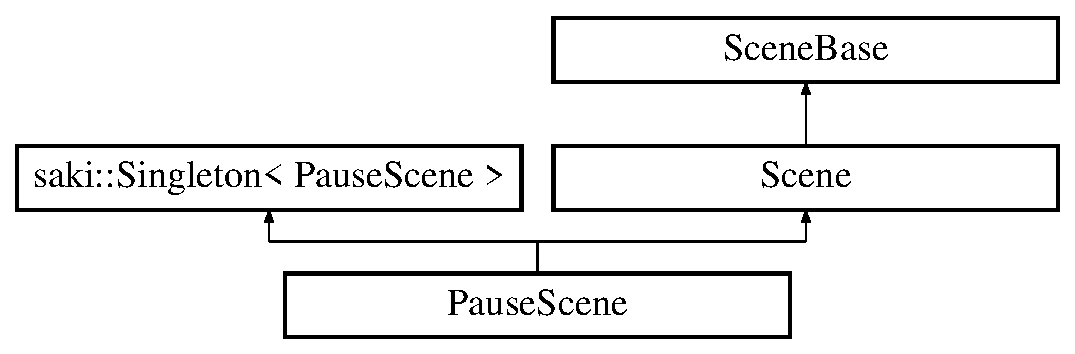
\includegraphics[height=3.000000cm]{class_pause_scene}
\end{center}
\end{figure}
\subsection*{公開メンバ関数}
\begin{DoxyCompactItemize}
\item 
void \mbox{\hyperlink{class_pause_scene_ad2df77966e0ac9ef6dfa99e416498183}{Init}} ()
\item 
std\+::shared\+\_\+ptr$<$ \mbox{\hyperlink{class_scene}{Scene}} $>$ \mbox{\hyperlink{class_pause_scene_a6adfe0685eb6bc64e658f6364c9f704d}{Update}} (std\+::shared\+\_\+ptr$<$ \mbox{\hyperlink{class_scene}{Scene}} $>$ \&)
\item 
void \mbox{\hyperlink{class_pause_scene_a4eeb70d814edbe91a10e315c5e9942df}{Render}} ()
\item 
void \mbox{\hyperlink{class_pause_scene_a1ff30a4006f7b93f13305b270bc0d913}{Destroy}} ()
\item 
void \mbox{\hyperlink{class_pause_scene_add74d9bcc744eaedbd6e8e10c5ee3bcc}{Reset}} ()
\item 
void \mbox{\hyperlink{class_pause_scene_a894f114f5398caf802eaad77826b7b2c}{End\+Pause}} ()
\item 
void \mbox{\hyperlink{class_pause_scene_acc1c366b69b6de802332b4e3d7993b41}{Switch\+Pause}} ()
\end{DoxyCompactItemize}
\subsection*{公開変数類}
\begin{DoxyCompactItemize}
\item 
bool \mbox{\hyperlink{class_pause_scene_ae6b7dfe712032062c6406a05cd258756}{is\+\_\+pause}} = false
\end{DoxyCompactItemize}
\subsection*{その他の継承メンバ}


\subsection{関数詳解}
\mbox{\Hypertarget{class_pause_scene_a1ff30a4006f7b93f13305b270bc0d913}\label{class_pause_scene_a1ff30a4006f7b93f13305b270bc0d913}} 
\index{Pause\+Scene@{Pause\+Scene}!Destroy@{Destroy}}
\index{Destroy@{Destroy}!Pause\+Scene@{Pause\+Scene}}
\subsubsection{\texorpdfstring{Destroy()}{Destroy()}}
{\footnotesize\ttfamily void Pause\+Scene\+::\+Destroy (\begin{DoxyParamCaption}{ }\end{DoxyParamCaption})\hspace{0.3cm}{\ttfamily [virtual]}}



\mbox{\hyperlink{class_scene_base_a7c5b54020bc519b4dadfe9770d6b27f7}{Scene\+Base}}を実装しています。

\mbox{\Hypertarget{class_pause_scene_a894f114f5398caf802eaad77826b7b2c}\label{class_pause_scene_a894f114f5398caf802eaad77826b7b2c}} 
\index{Pause\+Scene@{Pause\+Scene}!End\+Pause@{End\+Pause}}
\index{End\+Pause@{End\+Pause}!Pause\+Scene@{Pause\+Scene}}
\subsubsection{\texorpdfstring{End\+Pause()}{EndPause()}}
{\footnotesize\ttfamily void Pause\+Scene\+::\+End\+Pause (\begin{DoxyParamCaption}{ }\end{DoxyParamCaption})\hspace{0.3cm}{\ttfamily [inline]}}

\mbox{\Hypertarget{class_pause_scene_ad2df77966e0ac9ef6dfa99e416498183}\label{class_pause_scene_ad2df77966e0ac9ef6dfa99e416498183}} 
\index{Pause\+Scene@{Pause\+Scene}!Init@{Init}}
\index{Init@{Init}!Pause\+Scene@{Pause\+Scene}}
\subsubsection{\texorpdfstring{Init()}{Init()}}
{\footnotesize\ttfamily void Pause\+Scene\+::\+Init (\begin{DoxyParamCaption}{ }\end{DoxyParamCaption})\hspace{0.3cm}{\ttfamily [virtual]}}



\mbox{\hyperlink{class_scene_base_a24d7db43c819924dc8b07b436f6d3148}{Scene\+Base}}を実装しています。

\mbox{\Hypertarget{class_pause_scene_a4eeb70d814edbe91a10e315c5e9942df}\label{class_pause_scene_a4eeb70d814edbe91a10e315c5e9942df}} 
\index{Pause\+Scene@{Pause\+Scene}!Render@{Render}}
\index{Render@{Render}!Pause\+Scene@{Pause\+Scene}}
\subsubsection{\texorpdfstring{Render()}{Render()}}
{\footnotesize\ttfamily void Pause\+Scene\+::\+Render (\begin{DoxyParamCaption}{ }\end{DoxyParamCaption})\hspace{0.3cm}{\ttfamily [virtual]}}



\mbox{\hyperlink{class_scene_base_ad981674ce731ea267f398e889bbb9dc3}{Scene\+Base}}を実装しています。

\mbox{\Hypertarget{class_pause_scene_add74d9bcc744eaedbd6e8e10c5ee3bcc}\label{class_pause_scene_add74d9bcc744eaedbd6e8e10c5ee3bcc}} 
\index{Pause\+Scene@{Pause\+Scene}!Reset@{Reset}}
\index{Reset@{Reset}!Pause\+Scene@{Pause\+Scene}}
\subsubsection{\texorpdfstring{Reset()}{Reset()}}
{\footnotesize\ttfamily void Pause\+Scene\+::\+Reset (\begin{DoxyParamCaption}{ }\end{DoxyParamCaption})\hspace{0.3cm}{\ttfamily [inline]}}

\mbox{\Hypertarget{class_pause_scene_acc1c366b69b6de802332b4e3d7993b41}\label{class_pause_scene_acc1c366b69b6de802332b4e3d7993b41}} 
\index{Pause\+Scene@{Pause\+Scene}!Switch\+Pause@{Switch\+Pause}}
\index{Switch\+Pause@{Switch\+Pause}!Pause\+Scene@{Pause\+Scene}}
\subsubsection{\texorpdfstring{Switch\+Pause()}{SwitchPause()}}
{\footnotesize\ttfamily void Pause\+Scene\+::\+Switch\+Pause (\begin{DoxyParamCaption}{ }\end{DoxyParamCaption})\hspace{0.3cm}{\ttfamily [inline]}}

\mbox{\Hypertarget{class_pause_scene_a6adfe0685eb6bc64e658f6364c9f704d}\label{class_pause_scene_a6adfe0685eb6bc64e658f6364c9f704d}} 
\index{Pause\+Scene@{Pause\+Scene}!Update@{Update}}
\index{Update@{Update}!Pause\+Scene@{Pause\+Scene}}
\subsubsection{\texorpdfstring{Update()}{Update()}}
{\footnotesize\ttfamily std\+::shared\+\_\+ptr$<$ \mbox{\hyperlink{class_scene}{Scene}} $>$ Pause\+Scene\+::\+Update (\begin{DoxyParamCaption}\item[{std\+::shared\+\_\+ptr$<$ \mbox{\hyperlink{class_scene}{Scene}} $>$ \&}]{scene\+\_\+ptr }\end{DoxyParamCaption})\hspace{0.3cm}{\ttfamily [virtual]}}



\mbox{\hyperlink{class_scene_ab71ee5f19764b90c87b4574aa1cb1d25}{Scene}}を実装しています。



\subsection{メンバ詳解}
\mbox{\Hypertarget{class_pause_scene_ae6b7dfe712032062c6406a05cd258756}\label{class_pause_scene_ae6b7dfe712032062c6406a05cd258756}} 
\index{Pause\+Scene@{Pause\+Scene}!is\+\_\+pause@{is\+\_\+pause}}
\index{is\+\_\+pause@{is\+\_\+pause}!Pause\+Scene@{Pause\+Scene}}
\subsubsection{\texorpdfstring{is\+\_\+pause}{is\_pause}}
{\footnotesize\ttfamily bool Pause\+Scene\+::is\+\_\+pause = false}



このクラス詳解は次のファイルから抽出されました\+:\begin{DoxyCompactItemize}
\item 
C\+:/\+Users/tokir/\+Documents/\+Git\+Hub/\+Weapon\+Merchant\+Adventure/src/src/scene/pause/\mbox{\hyperlink{pause__scene_8h}{pause\+\_\+scene.\+h}}\item 
C\+:/\+Users/tokir/\+Documents/\+Git\+Hub/\+Weapon\+Merchant\+Adventure/src/src/scene/pause/\mbox{\hyperlink{pause__scene_8cpp}{pause\+\_\+scene.\+cpp}}\end{DoxyCompactItemize}

\hypertarget{class_player}{}\section{Player クラス}
\label{class_player}\index{Player@{Player}}


プレイヤークラス  




{\ttfamily \#include $<$player.\+h$>$}

Player の継承関係図\begin{figure}[H]
\begin{center}
\leavevmode
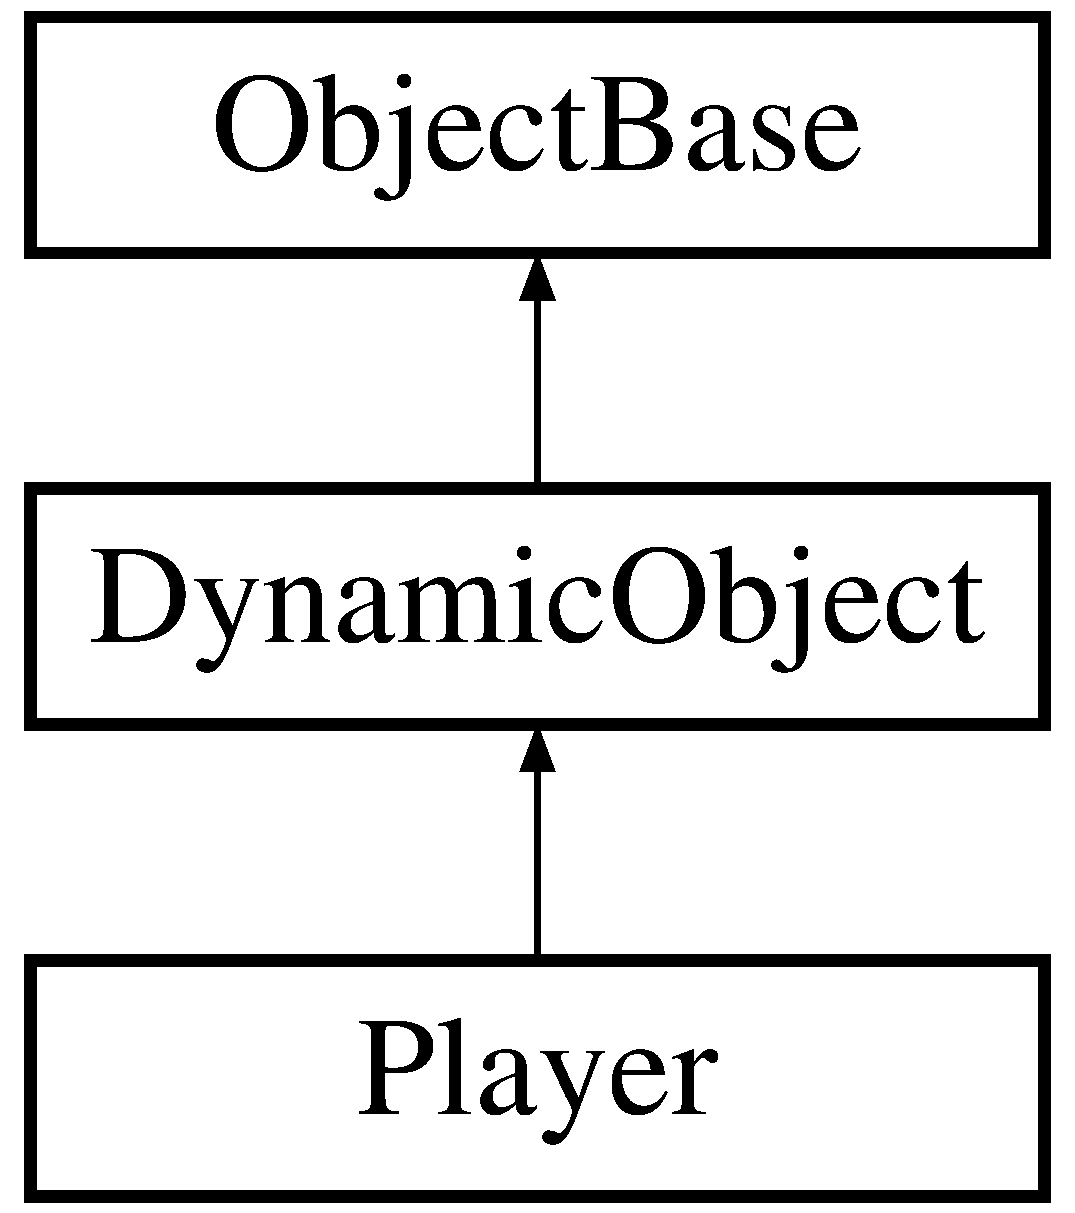
\includegraphics[height=3.000000cm]{class_player}
\end{center}
\end{figure}
\subsection*{公開メンバ関数}
\begin{DoxyCompactItemize}
\item 
void \mbox{\hyperlink{class_player_a848c2ecb62431010eaa9298b2c2c4be0}{Ui\+Render}} ()
\begin{DoxyCompactList}\small\item\em U\+Iの描画 \end{DoxyCompactList}\item 
void \mbox{\hyperlink{class_player_a615af41886fe293fcc3c6f276de77991}{Enabled\+Weapon}} ()
\begin{DoxyCompactList}\small\item\em 武器の非表示 \end{DoxyCompactList}\item 
void \mbox{\hyperlink{class_player_a97012a8b2bead252582ff39e852961ac}{Eenabled\+True\+Weapon}} ()
\begin{DoxyCompactList}\small\item\em 武器の表示 \end{DoxyCompactList}\item 
void \mbox{\hyperlink{class_player_a662de093359fb8e4a5bdc86a34fd2549}{Translation\+Boss\+Scene}} ()
\begin{DoxyCompactList}\small\item\em ボスシーンに移行するときの処理 \end{DoxyCompactList}\item 
void \mbox{\hyperlink{class_player_aff4d2bffe97e2b70f47f5eac2da26562}{In\+Boss\+Scene}} ()
\begin{DoxyCompactList}\small\item\em ボスシーンに入ったときの処理 \end{DoxyCompactList}\item 
void \mbox{\hyperlink{class_player_af1b9f4482efa53508befe6de204a3da6}{Animation\+Walk}} (bool right)
\begin{DoxyCompactList}\small\item\em 歩くアニメーションのみ関数化 \end{DoxyCompactList}\item 
void \mbox{\hyperlink{class_player_a8b27da2bdfb3e25337c7b6fd345d21f2}{Clear\+Update}} ()
\begin{DoxyCompactList}\small\item\em クリアした時の更新 \end{DoxyCompactList}\item 
void \mbox{\hyperlink{class_player_a6ddf26051788b56dd4029ba851e1f35a}{Reset\+Speed}} ()
\begin{DoxyCompactList}\small\item\em 横方向の力を0にする \end{DoxyCompactList}\item 
void \mbox{\hyperlink{class_player_af2cf4936165ef12cce96f7994e0879df}{Destroy}} () final
\begin{DoxyCompactList}\small\item\em プレイヤーの破棄 \end{DoxyCompactList}\item 
void \mbox{\hyperlink{class_player_abbb6662f1dc4ba3f75cafa6100160da0}{Update\+Animation}} (bool right=true)
\begin{DoxyCompactList}\small\item\em アニメーションの更新 \end{DoxyCompactList}\item 
\mbox{\hyperlink{class_player_affe0cc3cb714f6deb4e62f0c0d3f1fd8}{Player}} ()
\begin{DoxyCompactList}\small\item\em コンストラクタ \end{DoxyCompactList}\item 
\mbox{\hyperlink{class_player_a635af5e438af5a296c88f768e5e93eb0}{Player}} (\mbox{\hyperlink{class_player}{Player}} \&\&other) noexcept
\begin{DoxyCompactList}\small\item\em ムーブコンストラクタ \end{DoxyCompactList}\item 
\mbox{\hyperlink{class_player}{Player}} \& \mbox{\hyperlink{class_player_a8868988ae751daed5cfa32627e78889b}{operator=}} (const \mbox{\hyperlink{class_player}{Player}} \&other)
\begin{DoxyCompactList}\small\item\em コピー代入演算子 \end{DoxyCompactList}\item 
void \mbox{\hyperlink{class_player_a992b5c7e0d981308ed56706c6e71a709}{Collision}} (\mbox{\hyperlink{class_object_base}{Object\+Base}} $\ast$, \mbox{\hyperlink{common_8h_ae148fff5818e9444b4ab2288829559bf}{Vec2}}) final
\begin{DoxyCompactList}\small\item\em 当たってるときに実行する関数 \end{DoxyCompactList}\item 
void \mbox{\hyperlink{class_player_a6c879db24d39d894207e078eb4c56e8d}{Attack}} ()
\begin{DoxyCompactList}\small\item\em 攻撃 \end{DoxyCompactList}\end{DoxyCompactItemize}
\subsection*{公開変数類}
\begin{DoxyCompactItemize}
\item 
bool \mbox{\hyperlink{class_player_adf34c7a3a58c3f8e7f7201ed962a03f0}{boss\+\_\+scene}} = false
\end{DoxyCompactItemize}
\subsection*{限定公開メンバ関数}
\begin{DoxyCompactItemize}
\item 
void \mbox{\hyperlink{class_player_a1051f85c8bf18a256d275d1a1dee5da6}{Init\+Process}} () final
\begin{DoxyCompactList}\small\item\em 初期化 \end{DoxyCompactList}\item 
void \mbox{\hyperlink{class_player_ab8accc9b83b030f5313f1b4872a7e634}{Update\+Process}} () final
\begin{DoxyCompactList}\small\item\em プレイヤーの更新 \end{DoxyCompactList}\item 
void \mbox{\hyperlink{class_player_a8ac2e54fe5672d32186456b9735c02c3}{Render\+Process}} (bool camera\+\_\+affected) final
\begin{DoxyCompactList}\small\item\em プレイヤーの描画 \end{DoxyCompactList}\end{DoxyCompactItemize}
\subsection*{その他の継承メンバ}


\subsection{詳解}
プレイヤークラス 

\subsection{構築子と解体子}
\mbox{\Hypertarget{class_player_affe0cc3cb714f6deb4e62f0c0d3f1fd8}\label{class_player_affe0cc3cb714f6deb4e62f0c0d3f1fd8}} 
\index{Player@{Player}!Player@{Player}}
\index{Player@{Player}!Player@{Player}}
\subsubsection{\texorpdfstring{Player()}{Player()}\hspace{0.1cm}{\footnotesize\ttfamily [1/2]}}
{\footnotesize\ttfamily Player\+::\+Player (\begin{DoxyParamCaption}{ }\end{DoxyParamCaption})\hspace{0.3cm}{\ttfamily [inline]}}



コンストラクタ 

\mbox{\Hypertarget{class_player_a635af5e438af5a296c88f768e5e93eb0}\label{class_player_a635af5e438af5a296c88f768e5e93eb0}} 
\index{Player@{Player}!Player@{Player}}
\index{Player@{Player}!Player@{Player}}
\subsubsection{\texorpdfstring{Player()}{Player()}\hspace{0.1cm}{\footnotesize\ttfamily [2/2]}}
{\footnotesize\ttfamily Player\+::\+Player (\begin{DoxyParamCaption}\item[{\mbox{\hyperlink{class_player}{Player}} \&\&}]{other }\end{DoxyParamCaption})\hspace{0.3cm}{\ttfamily [inline]}, {\ttfamily [noexcept]}}



ムーブコンストラクタ 



\subsection{関数詳解}
\mbox{\Hypertarget{class_player_af1b9f4482efa53508befe6de204a3da6}\label{class_player_af1b9f4482efa53508befe6de204a3da6}} 
\index{Player@{Player}!Animation\+Walk@{Animation\+Walk}}
\index{Animation\+Walk@{Animation\+Walk}!Player@{Player}}
\subsubsection{\texorpdfstring{Animation\+Walk()}{AnimationWalk()}}
{\footnotesize\ttfamily void Player\+::\+Animation\+Walk (\begin{DoxyParamCaption}\item[{bool}]{right }\end{DoxyParamCaption})\hspace{0.3cm}{\ttfamily [inline]}}



歩くアニメーションのみ関数化 


\begin{DoxyParams}{引数}
{\em right} & 右かどうか \\
\hline
\end{DoxyParams}
\mbox{\Hypertarget{class_player_a6c879db24d39d894207e078eb4c56e8d}\label{class_player_a6c879db24d39d894207e078eb4c56e8d}} 
\index{Player@{Player}!Attack@{Attack}}
\index{Attack@{Attack}!Player@{Player}}
\subsubsection{\texorpdfstring{Attack()}{Attack()}}
{\footnotesize\ttfamily void Player\+::\+Attack (\begin{DoxyParamCaption}{ }\end{DoxyParamCaption})}



攻撃 

\mbox{\Hypertarget{class_player_a8b27da2bdfb3e25337c7b6fd345d21f2}\label{class_player_a8b27da2bdfb3e25337c7b6fd345d21f2}} 
\index{Player@{Player}!Clear\+Update@{Clear\+Update}}
\index{Clear\+Update@{Clear\+Update}!Player@{Player}}
\subsubsection{\texorpdfstring{Clear\+Update()}{ClearUpdate()}}
{\footnotesize\ttfamily void Player\+::\+Clear\+Update (\begin{DoxyParamCaption}{ }\end{DoxyParamCaption})\hspace{0.3cm}{\ttfamily [inline]}}



クリアした時の更新 

\mbox{\Hypertarget{class_player_a992b5c7e0d981308ed56706c6e71a709}\label{class_player_a992b5c7e0d981308ed56706c6e71a709}} 
\index{Player@{Player}!Collision@{Collision}}
\index{Collision@{Collision}!Player@{Player}}
\subsubsection{\texorpdfstring{Collision()}{Collision()}}
{\footnotesize\ttfamily void Player\+::\+Collision (\begin{DoxyParamCaption}\item[{\mbox{\hyperlink{class_object_base}{Object\+Base}} $\ast$}]{obj,  }\item[{\mbox{\hyperlink{common_8h_ae148fff5818e9444b4ab2288829559bf}{Vec2}}}]{ }\end{DoxyParamCaption})\hspace{0.3cm}{\ttfamily [final]}, {\ttfamily [virtual]}}



当たってるときに実行する関数 



\mbox{\hyperlink{class_object_base_a3e1db79dfa119be067d816c22d09839d}{Object\+Base}}を再実装しています。

\mbox{\Hypertarget{class_player_af2cf4936165ef12cce96f7994e0879df}\label{class_player_af2cf4936165ef12cce96f7994e0879df}} 
\index{Player@{Player}!Destroy@{Destroy}}
\index{Destroy@{Destroy}!Player@{Player}}
\subsubsection{\texorpdfstring{Destroy()}{Destroy()}}
{\footnotesize\ttfamily void Player\+::\+Destroy (\begin{DoxyParamCaption}{ }\end{DoxyParamCaption})\hspace{0.3cm}{\ttfamily [final]}, {\ttfamily [virtual]}}



プレイヤーの破棄 



\mbox{\hyperlink{class_object_base_a7fa4c548153c3af20f89673ffea809af}{Object\+Base}}を実装しています。

\mbox{\Hypertarget{class_player_a97012a8b2bead252582ff39e852961ac}\label{class_player_a97012a8b2bead252582ff39e852961ac}} 
\index{Player@{Player}!Eenabled\+True\+Weapon@{Eenabled\+True\+Weapon}}
\index{Eenabled\+True\+Weapon@{Eenabled\+True\+Weapon}!Player@{Player}}
\subsubsection{\texorpdfstring{Eenabled\+True\+Weapon()}{EenabledTrueWeapon()}}
{\footnotesize\ttfamily void Player\+::\+Eenabled\+True\+Weapon (\begin{DoxyParamCaption}{ }\end{DoxyParamCaption})\hspace{0.3cm}{\ttfamily [inline]}}



武器の表示 

\mbox{\Hypertarget{class_player_a615af41886fe293fcc3c6f276de77991}\label{class_player_a615af41886fe293fcc3c6f276de77991}} 
\index{Player@{Player}!Enabled\+Weapon@{Enabled\+Weapon}}
\index{Enabled\+Weapon@{Enabled\+Weapon}!Player@{Player}}
\subsubsection{\texorpdfstring{Enabled\+Weapon()}{EnabledWeapon()}}
{\footnotesize\ttfamily void Player\+::\+Enabled\+Weapon (\begin{DoxyParamCaption}{ }\end{DoxyParamCaption})\hspace{0.3cm}{\ttfamily [inline]}}



武器の非表示 

\mbox{\Hypertarget{class_player_aff4d2bffe97e2b70f47f5eac2da26562}\label{class_player_aff4d2bffe97e2b70f47f5eac2da26562}} 
\index{Player@{Player}!In\+Boss\+Scene@{In\+Boss\+Scene}}
\index{In\+Boss\+Scene@{In\+Boss\+Scene}!Player@{Player}}
\subsubsection{\texorpdfstring{In\+Boss\+Scene()}{InBossScene()}}
{\footnotesize\ttfamily void Player\+::\+In\+Boss\+Scene (\begin{DoxyParamCaption}{ }\end{DoxyParamCaption})\hspace{0.3cm}{\ttfamily [inline]}}



ボスシーンに入ったときの処理 

\mbox{\Hypertarget{class_player_a1051f85c8bf18a256d275d1a1dee5da6}\label{class_player_a1051f85c8bf18a256d275d1a1dee5da6}} 
\index{Player@{Player}!Init\+Process@{Init\+Process}}
\index{Init\+Process@{Init\+Process}!Player@{Player}}
\subsubsection{\texorpdfstring{Init\+Process()}{InitProcess()}}
{\footnotesize\ttfamily void Player\+::\+Init\+Process (\begin{DoxyParamCaption}{ }\end{DoxyParamCaption})\hspace{0.3cm}{\ttfamily [final]}, {\ttfamily [protected]}, {\ttfamily [virtual]}}



初期化 



\mbox{\hyperlink{class_object_base_af133f36f2bca1dcfd962e2cfac61ab51}{Object\+Base}}を実装しています。

\mbox{\Hypertarget{class_player_a8868988ae751daed5cfa32627e78889b}\label{class_player_a8868988ae751daed5cfa32627e78889b}} 
\index{Player@{Player}!operator=@{operator=}}
\index{operator=@{operator=}!Player@{Player}}
\subsubsection{\texorpdfstring{operator=()}{operator=()}}
{\footnotesize\ttfamily \mbox{\hyperlink{class_player}{Player}}\& Player\+::operator= (\begin{DoxyParamCaption}\item[{const \mbox{\hyperlink{class_player}{Player}} \&}]{other }\end{DoxyParamCaption})\hspace{0.3cm}{\ttfamily [inline]}}



コピー代入演算子 

\mbox{\Hypertarget{class_player_a8ac2e54fe5672d32186456b9735c02c3}\label{class_player_a8ac2e54fe5672d32186456b9735c02c3}} 
\index{Player@{Player}!Render\+Process@{Render\+Process}}
\index{Render\+Process@{Render\+Process}!Player@{Player}}
\subsubsection{\texorpdfstring{Render\+Process()}{RenderProcess()}}
{\footnotesize\ttfamily void Player\+::\+Render\+Process (\begin{DoxyParamCaption}\item[{bool}]{camera\+\_\+affected }\end{DoxyParamCaption})\hspace{0.3cm}{\ttfamily [final]}, {\ttfamily [protected]}, {\ttfamily [virtual]}}



プレイヤーの描画 


\begin{DoxyParams}{引数}
{\em camera\+\_\+affected} & カメラの位置によって描画する位置を変えるかどうか \\
\hline
\end{DoxyParams}


\mbox{\hyperlink{class_dynamic_object_aa7488e1b4dfd7049447535d93d9d6783}{Dynamic\+Object}}を再実装しています。

\mbox{\Hypertarget{class_player_a6ddf26051788b56dd4029ba851e1f35a}\label{class_player_a6ddf26051788b56dd4029ba851e1f35a}} 
\index{Player@{Player}!Reset\+Speed@{Reset\+Speed}}
\index{Reset\+Speed@{Reset\+Speed}!Player@{Player}}
\subsubsection{\texorpdfstring{Reset\+Speed()}{ResetSpeed()}}
{\footnotesize\ttfamily void Player\+::\+Reset\+Speed (\begin{DoxyParamCaption}{ }\end{DoxyParamCaption})\hspace{0.3cm}{\ttfamily [inline]}}



横方向の力を0にする 

\mbox{\Hypertarget{class_player_a662de093359fb8e4a5bdc86a34fd2549}\label{class_player_a662de093359fb8e4a5bdc86a34fd2549}} 
\index{Player@{Player}!Translation\+Boss\+Scene@{Translation\+Boss\+Scene}}
\index{Translation\+Boss\+Scene@{Translation\+Boss\+Scene}!Player@{Player}}
\subsubsection{\texorpdfstring{Translation\+Boss\+Scene()}{TranslationBossScene()}}
{\footnotesize\ttfamily void Player\+::\+Translation\+Boss\+Scene (\begin{DoxyParamCaption}{ }\end{DoxyParamCaption})\hspace{0.3cm}{\ttfamily [inline]}}



ボスシーンに移行するときの処理 

\mbox{\Hypertarget{class_player_a848c2ecb62431010eaa9298b2c2c4be0}\label{class_player_a848c2ecb62431010eaa9298b2c2c4be0}} 
\index{Player@{Player}!Ui\+Render@{Ui\+Render}}
\index{Ui\+Render@{Ui\+Render}!Player@{Player}}
\subsubsection{\texorpdfstring{Ui\+Render()}{UiRender()}}
{\footnotesize\ttfamily void Player\+::\+Ui\+Render (\begin{DoxyParamCaption}{ }\end{DoxyParamCaption})}



U\+Iの描画 

\mbox{\Hypertarget{class_player_abbb6662f1dc4ba3f75cafa6100160da0}\label{class_player_abbb6662f1dc4ba3f75cafa6100160da0}} 
\index{Player@{Player}!Update\+Animation@{Update\+Animation}}
\index{Update\+Animation@{Update\+Animation}!Player@{Player}}
\subsubsection{\texorpdfstring{Update\+Animation()}{UpdateAnimation()}}
{\footnotesize\ttfamily void Player\+::\+Update\+Animation (\begin{DoxyParamCaption}\item[{bool}]{right = {\ttfamily true} }\end{DoxyParamCaption})\hspace{0.3cm}{\ttfamily [inline]}}



アニメーションの更新 

\mbox{\Hypertarget{class_player_ab8accc9b83b030f5313f1b4872a7e634}\label{class_player_ab8accc9b83b030f5313f1b4872a7e634}} 
\index{Player@{Player}!Update\+Process@{Update\+Process}}
\index{Update\+Process@{Update\+Process}!Player@{Player}}
\subsubsection{\texorpdfstring{Update\+Process()}{UpdateProcess()}}
{\footnotesize\ttfamily void Player\+::\+Update\+Process (\begin{DoxyParamCaption}{ }\end{DoxyParamCaption})\hspace{0.3cm}{\ttfamily [final]}, {\ttfamily [protected]}, {\ttfamily [virtual]}}



プレイヤーの更新 



\mbox{\hyperlink{class_object_base_a8b5b72b363a419767efde0b0e692ea95}{Object\+Base}}を実装しています。



\subsection{メンバ詳解}
\mbox{\Hypertarget{class_player_adf34c7a3a58c3f8e7f7201ed962a03f0}\label{class_player_adf34c7a3a58c3f8e7f7201ed962a03f0}} 
\index{Player@{Player}!boss\+\_\+scene@{boss\+\_\+scene}}
\index{boss\+\_\+scene@{boss\+\_\+scene}!Player@{Player}}
\subsubsection{\texorpdfstring{boss\+\_\+scene}{boss\_scene}}
{\footnotesize\ttfamily bool Player\+::boss\+\_\+scene = false}



このクラス詳解は次のファイルから抽出されました\+:\begin{DoxyCompactItemize}
\item 
C\+:/\+Users/tokir/\+Documents/\+Git\+Hub/\+Weapon\+Merchant\+Adventure/src/src/object/character/player/\mbox{\hyperlink{player_8h}{player.\+h}}\item 
C\+:/\+Users/tokir/\+Documents/\+Git\+Hub/\+Weapon\+Merchant\+Adventure/src/src/object/character/player/\mbox{\hyperlink{player_8cpp}{player.\+cpp}}\end{DoxyCompactItemize}

\hypertarget{structsaki_1_1_return_param}{}\section{saki\+:\+:Return\+Param 構造体}
\label{structsaki_1_1_return_param}\index{saki\+::\+Return\+Param@{saki\+::\+Return\+Param}}


そのまま引数を返す関数オブジェクト  




{\ttfamily \#include $<$return\+\_\+param.\+h$>$}

\subsection*{公開メンバ関数}
\begin{DoxyCompactItemize}
\item 
{\footnotesize template$<$typename T $>$ }\\constexpr T \mbox{\hyperlink{structsaki_1_1_return_param_aac580f81f20f20e1f29cb17992e1520b}{operator()}} (const T \&t) const
\end{DoxyCompactItemize}


\subsection{詳解}
そのまま引数を返す関数オブジェクト 

\subsection{関数詳解}
\mbox{\Hypertarget{structsaki_1_1_return_param_aac580f81f20f20e1f29cb17992e1520b}\label{structsaki_1_1_return_param_aac580f81f20f20e1f29cb17992e1520b}} 
\index{saki\+::\+Return\+Param@{saki\+::\+Return\+Param}!operator()@{operator()}}
\index{operator()@{operator()}!saki\+::\+Return\+Param@{saki\+::\+Return\+Param}}
\subsubsection{\texorpdfstring{operator()()}{operator()()}}
{\footnotesize\ttfamily template$<$typename T $>$ \\
constexpr T saki\+::\+Return\+Param\+::operator() (\begin{DoxyParamCaption}\item[{const T \&}]{t }\end{DoxyParamCaption}) const\hspace{0.3cm}{\ttfamily [inline]}}



この構造体詳解は次のファイルから抽出されました\+:\begin{DoxyCompactItemize}
\item 
C\+:/\+Users/tokir/\+Documents/\+Git\+Hub/\+Weapon\+Merchant\+Adventure/src/lib/saki/binary\+\_\+operator/\mbox{\hyperlink{return__param_8h}{return\+\_\+param.\+h}}\end{DoxyCompactItemize}

\hypertarget{class_scene}{}\section{Scene クラス}
\label{class_scene}\index{Scene@{Scene}}


マネージャーを含まないシーンのスーパークラス  




{\ttfamily \#include $<$scene.\+h$>$}

Scene の継承関係図\begin{figure}[H]
\begin{center}
\leavevmode
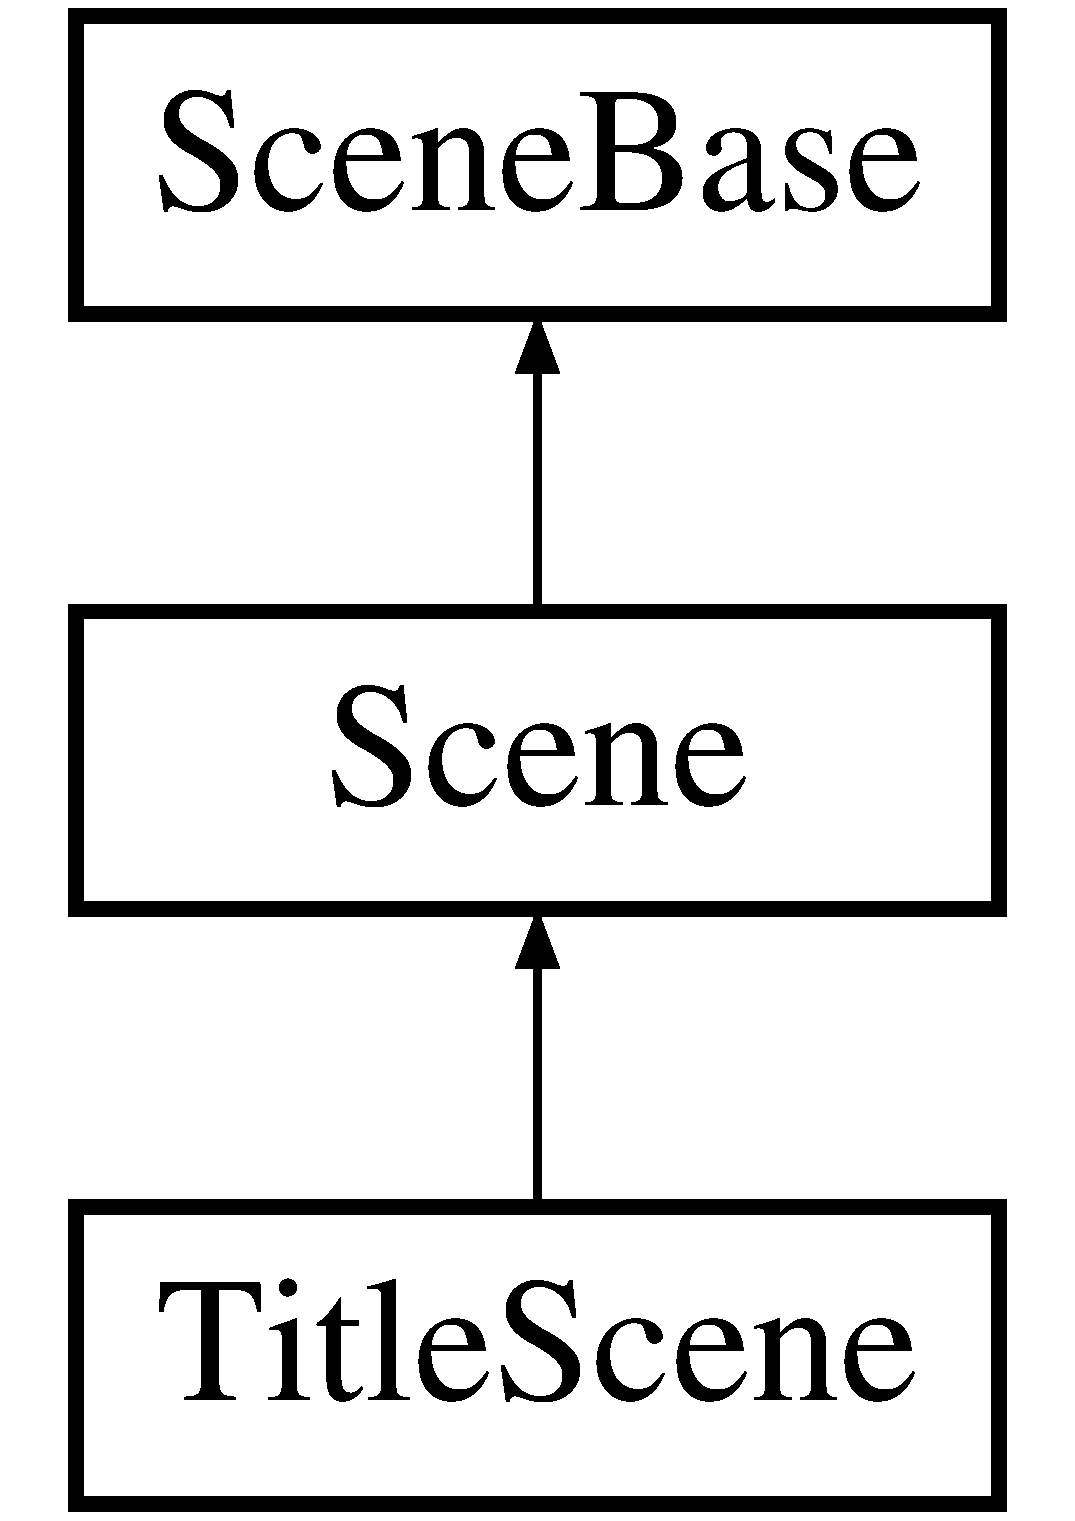
\includegraphics[height=1.875000cm]{class_scene}
\end{center}
\end{figure}
\subsection*{公開メンバ関数}
\begin{DoxyCompactItemize}
\item 
virtual \mbox{\hyperlink{class_scene_aa0a5be58e2ee2d1fdafc5fb46b5e661e}{$\sim$\+Scene}} ()
\item 
virtual std\+::shared\+\_\+ptr$<$ \mbox{\hyperlink{class_scene}{Scene}} $>$ \mbox{\hyperlink{class_scene_ab71ee5f19764b90c87b4574aa1cb1d25}{Update}} (std\+::shared\+\_\+ptr$<$ \mbox{\hyperlink{class_scene}{Scene}} $>$ \&)=0
\item 
virtual void \mbox{\hyperlink{class_scene_ad19a449c6ed452823dae14183689570c}{Exit\+Fade\+Update}} ()
\begin{DoxyCompactList}\small\item\em シーンが変わるときの更新 \end{DoxyCompactList}\end{DoxyCompactItemize}


\subsection{詳解}
マネージャーを含まないシーンのスーパークラス 

マネージャーはこのクラスを保持する 

\subsection{構築子と解体子}
\mbox{\Hypertarget{class_scene_aa0a5be58e2ee2d1fdafc5fb46b5e661e}\label{class_scene_aa0a5be58e2ee2d1fdafc5fb46b5e661e}} 
\index{Scene@{Scene}!````~Scene@{$\sim$\+Scene}}
\index{````~Scene@{$\sim$\+Scene}!Scene@{Scene}}
\subsubsection{\texorpdfstring{$\sim$\+Scene()}{~Scene()}}
{\footnotesize\ttfamily virtual Scene\+::$\sim$\+Scene (\begin{DoxyParamCaption}{ }\end{DoxyParamCaption})\hspace{0.3cm}{\ttfamily [inline]}, {\ttfamily [virtual]}}



\subsection{関数詳解}
\mbox{\Hypertarget{class_scene_ad19a449c6ed452823dae14183689570c}\label{class_scene_ad19a449c6ed452823dae14183689570c}} 
\index{Scene@{Scene}!Exit\+Fade\+Update@{Exit\+Fade\+Update}}
\index{Exit\+Fade\+Update@{Exit\+Fade\+Update}!Scene@{Scene}}
\subsubsection{\texorpdfstring{Exit\+Fade\+Update()}{ExitFadeUpdate()}}
{\footnotesize\ttfamily virtual void Scene\+::\+Exit\+Fade\+Update (\begin{DoxyParamCaption}{ }\end{DoxyParamCaption})\hspace{0.3cm}{\ttfamily [inline]}, {\ttfamily [virtual]}}



シーンが変わるときの更新 



\mbox{\hyperlink{class_select_scene_a546190bc143f6d7a3055935f97b55596}{Select\+Scene}}で再実装されています。

\mbox{\Hypertarget{class_scene_ab71ee5f19764b90c87b4574aa1cb1d25}\label{class_scene_ab71ee5f19764b90c87b4574aa1cb1d25}} 
\index{Scene@{Scene}!Update@{Update}}
\index{Update@{Update}!Scene@{Scene}}
\subsubsection{\texorpdfstring{Update()}{Update()}}
{\footnotesize\ttfamily virtual std\+::shared\+\_\+ptr$<$\mbox{\hyperlink{class_scene}{Scene}}$>$ Scene\+::\+Update (\begin{DoxyParamCaption}\item[{std\+::shared\+\_\+ptr$<$ \mbox{\hyperlink{class_scene}{Scene}} $>$ \&}]{ }\end{DoxyParamCaption})\hspace{0.3cm}{\ttfamily [pure virtual]}}



\mbox{\hyperlink{class_select_scene_a0cef696ddf74155e061cc5f9f2e06419}{Select\+Scene}}, \mbox{\hyperlink{class_title_scene_ab3097e96e2fe65d6fad0d6bb45a14f9f}{Title\+Scene}}, \mbox{\hyperlink{class_pause_scene_a6adfe0685eb6bc64e658f6364c9f704d}{Pause\+Scene}}, \mbox{\hyperlink{class_game_scene_easy_ac2bccbf61722010fd6f317693ee7b8b1}{Game\+Scene\+Easy}}, \mbox{\hyperlink{class_game_scene_hard_ac132a0e281a7d4e6b71deb6e5bcfdb9d}{Game\+Scene\+Hard}}, \mbox{\hyperlink{class_game_scene_normal_a3e45ac3882f1d0dd5c77ab4f0a1ccb33}{Game\+Scene\+Normal}}, \mbox{\hyperlink{class_exit_scene_a18655f3124150a911f266e66e3fc4480}{Exit\+Scene}}で実装されています。



このクラス詳解は次のファイルから抽出されました\+:\begin{DoxyCompactItemize}
\item 
C\+:/\+Users/tokir/\+Documents/\+Git\+Hub/\+Weapon\+Merchant\+Adventure/src/src/scene/\mbox{\hyperlink{scene_8h}{scene.\+h}}\end{DoxyCompactItemize}

\hypertarget{class_scene_base}{}\section{Scene\+Base クラス}
\label{class_scene_base}\index{Scene\+Base@{Scene\+Base}}


マネージャーを含むシーンのスーパークラス  




{\ttfamily \#include $<$scene\+\_\+base.\+h$>$}

Scene\+Base の継承関係図\begin{figure}[H]
\begin{center}
\leavevmode
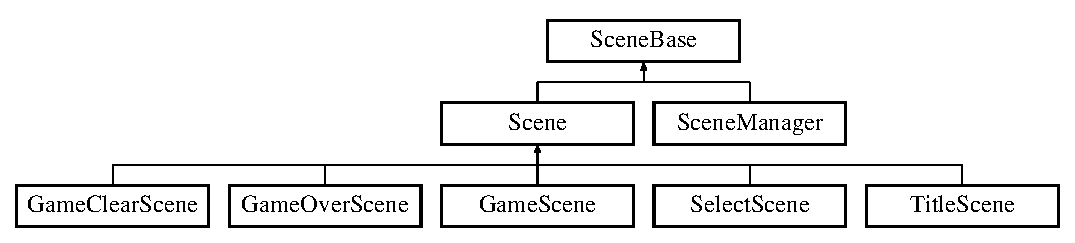
\includegraphics[height=3.000000cm]{class_scene_base}
\end{center}
\end{figure}
\subsection*{公開メンバ関数}
\begin{DoxyCompactItemize}
\item 
virtual \mbox{\hyperlink{class_scene_base_a187dd160e5a16909bcc6529851e38318}{$\sim$\+Scene\+Base}} ()
\item 
virtual void \mbox{\hyperlink{class_scene_base_a24d7db43c819924dc8b07b436f6d3148}{Init}} ()=0
\item 
virtual void \mbox{\hyperlink{class_scene_base_ad981674ce731ea267f398e889bbb9dc3}{Render}} ()=0
\item 
virtual void \mbox{\hyperlink{class_scene_base_a7c5b54020bc519b4dadfe9770d6b27f7}{Destroy}} ()=0
\end{DoxyCompactItemize}
\subsection*{限定公開変数類}
\begin{DoxyCompactItemize}
\item 
\mbox{\hyperlink{scene__base_8h_a24cee5343fb9d0706ead6e8601f363be}{S\+C\+E\+NE}} \mbox{\hyperlink{class_scene_base_a18dcdbacfbd98f73099c3cbeb70ae3b8}{my\+\_\+scene}}
\end{DoxyCompactItemize}


\subsection{詳解}
マネージャーを含むシーンのスーパークラス 

\subsection{構築子と解体子}
\mbox{\Hypertarget{class_scene_base_a187dd160e5a16909bcc6529851e38318}\label{class_scene_base_a187dd160e5a16909bcc6529851e38318}} 
\index{Scene\+Base@{Scene\+Base}!````~Scene\+Base@{$\sim$\+Scene\+Base}}
\index{````~Scene\+Base@{$\sim$\+Scene\+Base}!Scene\+Base@{Scene\+Base}}
\subsubsection{\texorpdfstring{$\sim$\+Scene\+Base()}{~SceneBase()}}
{\footnotesize\ttfamily virtual Scene\+Base\+::$\sim$\+Scene\+Base (\begin{DoxyParamCaption}{ }\end{DoxyParamCaption})\hspace{0.3cm}{\ttfamily [inline]}, {\ttfamily [virtual]}}



\subsection{関数詳解}
\mbox{\Hypertarget{class_scene_base_a7c5b54020bc519b4dadfe9770d6b27f7}\label{class_scene_base_a7c5b54020bc519b4dadfe9770d6b27f7}} 
\index{Scene\+Base@{Scene\+Base}!Destroy@{Destroy}}
\index{Destroy@{Destroy}!Scene\+Base@{Scene\+Base}}
\subsubsection{\texorpdfstring{Destroy()}{Destroy()}}
{\footnotesize\ttfamily virtual void Scene\+Base\+::\+Destroy (\begin{DoxyParamCaption}{ }\end{DoxyParamCaption})\hspace{0.3cm}{\ttfamily [pure virtual]}}



\mbox{\hyperlink{class_title_scene_adfbc5f934572ede2e36419b089c88fe8}{Title\+Scene}}, \mbox{\hyperlink{class_scene_manager_a0e3ad11342e763f0d4108c0b4674a157}{Scene\+Manager}}で実装されています。

\mbox{\Hypertarget{class_scene_base_a24d7db43c819924dc8b07b436f6d3148}\label{class_scene_base_a24d7db43c819924dc8b07b436f6d3148}} 
\index{Scene\+Base@{Scene\+Base}!Init@{Init}}
\index{Init@{Init}!Scene\+Base@{Scene\+Base}}
\subsubsection{\texorpdfstring{Init()}{Init()}}
{\footnotesize\ttfamily virtual void Scene\+Base\+::\+Init (\begin{DoxyParamCaption}{ }\end{DoxyParamCaption})\hspace{0.3cm}{\ttfamily [pure virtual]}}



\mbox{\hyperlink{class_title_scene_a3d039e7db0fa1e22e8c36d3cedfbd318}{Title\+Scene}}, \mbox{\hyperlink{class_scene_manager_a6c0e84d0e76f23fb3172839dba5f091b}{Scene\+Manager}}で実装されています。

\mbox{\Hypertarget{class_scene_base_ad981674ce731ea267f398e889bbb9dc3}\label{class_scene_base_ad981674ce731ea267f398e889bbb9dc3}} 
\index{Scene\+Base@{Scene\+Base}!Render@{Render}}
\index{Render@{Render}!Scene\+Base@{Scene\+Base}}
\subsubsection{\texorpdfstring{Render()}{Render()}}
{\footnotesize\ttfamily virtual void Scene\+Base\+::\+Render (\begin{DoxyParamCaption}{ }\end{DoxyParamCaption})\hspace{0.3cm}{\ttfamily [pure virtual]}}



\mbox{\hyperlink{class_title_scene_af12c59b3bf9458640938c5ca620527ae}{Title\+Scene}}, \mbox{\hyperlink{class_scene_manager_a968ae7a0065b793f139bda6bcc58d106}{Scene\+Manager}}で実装されています。



\subsection{メンバ詳解}
\mbox{\Hypertarget{class_scene_base_a18dcdbacfbd98f73099c3cbeb70ae3b8}\label{class_scene_base_a18dcdbacfbd98f73099c3cbeb70ae3b8}} 
\index{Scene\+Base@{Scene\+Base}!my\+\_\+scene@{my\+\_\+scene}}
\index{my\+\_\+scene@{my\+\_\+scene}!Scene\+Base@{Scene\+Base}}
\subsubsection{\texorpdfstring{my\+\_\+scene}{my\_scene}}
{\footnotesize\ttfamily \mbox{\hyperlink{scene__base_8h_a24cee5343fb9d0706ead6e8601f363be}{S\+C\+E\+NE}} Scene\+Base\+::my\+\_\+scene\hspace{0.3cm}{\ttfamily [protected]}}



このクラス詳解は次のファイルから抽出されました\+:\begin{DoxyCompactItemize}
\item 
C\+:/\+Users/tokir/\+Documents/\+Git\+Hub/\+Weapon\+Merchant\+Adventure/src/scene/base/\mbox{\hyperlink{scene__base_8h}{scene\+\_\+base.\+h}}\end{DoxyCompactItemize}

\hypertarget{class_scene_manager}{}\section{Scene\+Manager クラス}
\label{class_scene_manager}\index{Scene\+Manager@{Scene\+Manager}}


シーンをマネージャーするクラス  




{\ttfamily \#include $<$scene\+\_\+manager.\+h$>$}

Scene\+Manager の継承関係図\begin{figure}[H]
\begin{center}
\leavevmode
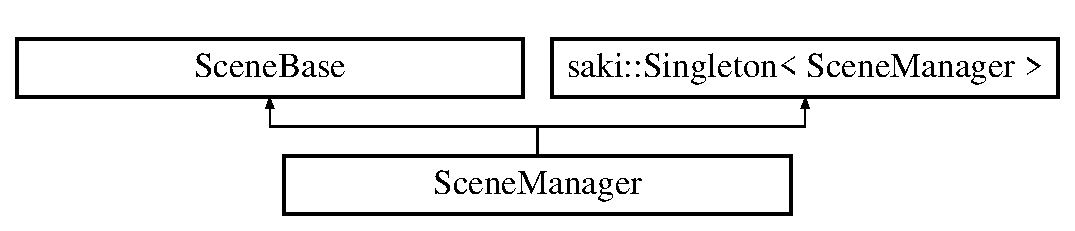
\includegraphics[height=2.000000cm]{class_scene_manager}
\end{center}
\end{figure}
\subsection*{公開メンバ関数}
\begin{DoxyCompactItemize}
\item 
void \mbox{\hyperlink{class_scene_manager_a6c0e84d0e76f23fb3172839dba5f091b}{Init}} () final
\begin{DoxyCompactList}\small\item\em シーンマネージャーの初期化 \end{DoxyCompactList}\item 
void \mbox{\hyperlink{class_scene_manager_a63dcf65832d6a2c190bf496d9a3b00a3}{Update}} ()
\begin{DoxyCompactList}\small\item\em 保持してるシーンの更新 \end{DoxyCompactList}\item 
void \mbox{\hyperlink{class_scene_manager_a968ae7a0065b793f139bda6bcc58d106}{Render}} () final
\begin{DoxyCompactList}\small\item\em 保持してるシーンの描画 \end{DoxyCompactList}\item 
void \mbox{\hyperlink{class_scene_manager_a0e3ad11342e763f0d4108c0b4674a157}{Destroy}} () final
\begin{DoxyCompactList}\small\item\em 保持してるシーンのマネージャーの破棄 \end{DoxyCompactList}\item 
void \mbox{\hyperlink{class_scene_manager_a5ed223ec14c6b62d378b3f95ed4f5d8e}{Continue\+Game}} (std\+::shared\+\_\+ptr$<$ \mbox{\hyperlink{class_scene}{Scene}} $>$ \&p)
\end{DoxyCompactItemize}
\subsection*{公開変数類}
\begin{DoxyCompactItemize}
\item 
bool \mbox{\hyperlink{class_scene_manager_a416645f4b11ce8cdb81d9d43d1c5666b}{is\+\_\+game\+\_\+scene}} = false
\end{DoxyCompactItemize}
\subsection*{その他の継承メンバ}


\subsection{詳解}
シーンをマネージャーするクラス 

\subsection{関数詳解}
\mbox{\Hypertarget{class_scene_manager_a5ed223ec14c6b62d378b3f95ed4f5d8e}\label{class_scene_manager_a5ed223ec14c6b62d378b3f95ed4f5d8e}} 
\index{Scene\+Manager@{Scene\+Manager}!Continue\+Game@{Continue\+Game}}
\index{Continue\+Game@{Continue\+Game}!Scene\+Manager@{Scene\+Manager}}
\subsubsection{\texorpdfstring{Continue\+Game()}{ContinueGame()}}
{\footnotesize\ttfamily void Scene\+Manager\+::\+Continue\+Game (\begin{DoxyParamCaption}\item[{std\+::shared\+\_\+ptr$<$ \mbox{\hyperlink{class_scene}{Scene}} $>$ \&}]{p }\end{DoxyParamCaption})\hspace{0.3cm}{\ttfamily [inline]}}

\mbox{\Hypertarget{class_scene_manager_a0e3ad11342e763f0d4108c0b4674a157}\label{class_scene_manager_a0e3ad11342e763f0d4108c0b4674a157}} 
\index{Scene\+Manager@{Scene\+Manager}!Destroy@{Destroy}}
\index{Destroy@{Destroy}!Scene\+Manager@{Scene\+Manager}}
\subsubsection{\texorpdfstring{Destroy()}{Destroy()}}
{\footnotesize\ttfamily void Scene\+Manager\+::\+Destroy (\begin{DoxyParamCaption}{ }\end{DoxyParamCaption})\hspace{0.3cm}{\ttfamily [final]}, {\ttfamily [virtual]}}



保持してるシーンのマネージャーの破棄 



\mbox{\hyperlink{class_scene_base_a7c5b54020bc519b4dadfe9770d6b27f7}{Scene\+Base}}を実装しています。

\mbox{\Hypertarget{class_scene_manager_a6c0e84d0e76f23fb3172839dba5f091b}\label{class_scene_manager_a6c0e84d0e76f23fb3172839dba5f091b}} 
\index{Scene\+Manager@{Scene\+Manager}!Init@{Init}}
\index{Init@{Init}!Scene\+Manager@{Scene\+Manager}}
\subsubsection{\texorpdfstring{Init()}{Init()}}
{\footnotesize\ttfamily void Scene\+Manager\+::\+Init (\begin{DoxyParamCaption}{ }\end{DoxyParamCaption})\hspace{0.3cm}{\ttfamily [final]}, {\ttfamily [virtual]}}



シーンマネージャーの初期化 



\mbox{\hyperlink{class_scene_base_a24d7db43c819924dc8b07b436f6d3148}{Scene\+Base}}を実装しています。

\mbox{\Hypertarget{class_scene_manager_a968ae7a0065b793f139bda6bcc58d106}\label{class_scene_manager_a968ae7a0065b793f139bda6bcc58d106}} 
\index{Scene\+Manager@{Scene\+Manager}!Render@{Render}}
\index{Render@{Render}!Scene\+Manager@{Scene\+Manager}}
\subsubsection{\texorpdfstring{Render()}{Render()}}
{\footnotesize\ttfamily void Scene\+Manager\+::\+Render (\begin{DoxyParamCaption}{ }\end{DoxyParamCaption})\hspace{0.3cm}{\ttfamily [final]}, {\ttfamily [virtual]}}



保持してるシーンの描画 



\mbox{\hyperlink{class_scene_base_ad981674ce731ea267f398e889bbb9dc3}{Scene\+Base}}を実装しています。

\mbox{\Hypertarget{class_scene_manager_a63dcf65832d6a2c190bf496d9a3b00a3}\label{class_scene_manager_a63dcf65832d6a2c190bf496d9a3b00a3}} 
\index{Scene\+Manager@{Scene\+Manager}!Update@{Update}}
\index{Update@{Update}!Scene\+Manager@{Scene\+Manager}}
\subsubsection{\texorpdfstring{Update()}{Update()}}
{\footnotesize\ttfamily void Scene\+Manager\+::\+Update (\begin{DoxyParamCaption}{ }\end{DoxyParamCaption})}



保持してるシーンの更新 



\subsection{メンバ詳解}
\mbox{\Hypertarget{class_scene_manager_a416645f4b11ce8cdb81d9d43d1c5666b}\label{class_scene_manager_a416645f4b11ce8cdb81d9d43d1c5666b}} 
\index{Scene\+Manager@{Scene\+Manager}!is\+\_\+game\+\_\+scene@{is\+\_\+game\+\_\+scene}}
\index{is\+\_\+game\+\_\+scene@{is\+\_\+game\+\_\+scene}!Scene\+Manager@{Scene\+Manager}}
\subsubsection{\texorpdfstring{is\+\_\+game\+\_\+scene}{is\_game\_scene}}
{\footnotesize\ttfamily bool Scene\+Manager\+::is\+\_\+game\+\_\+scene = false}



このクラス詳解は次のファイルから抽出されました\+:\begin{DoxyCompactItemize}
\item 
C\+:/\+Users/tokir/\+Documents/\+Git\+Hub/\+Weapon\+Merchant\+Adventure/src/src/scene/manager/\mbox{\hyperlink{scene__manager_8h}{scene\+\_\+manager.\+h}}\item 
C\+:/\+Users/tokir/\+Documents/\+Git\+Hub/\+Weapon\+Merchant\+Adventure/src/src/scene/manager/\mbox{\hyperlink{scene__manager_8cpp}{scene\+\_\+manager.\+cpp}}\end{DoxyCompactItemize}

\hypertarget{class_select_obj}{}\section{Select\+Obj クラス}
\label{class_select_obj}\index{Select\+Obj@{Select\+Obj}}


{\ttfamily \#include $<$select\+\_\+object.\+h$>$}

Select\+Obj の継承関係図\begin{figure}[H]
\begin{center}
\leavevmode
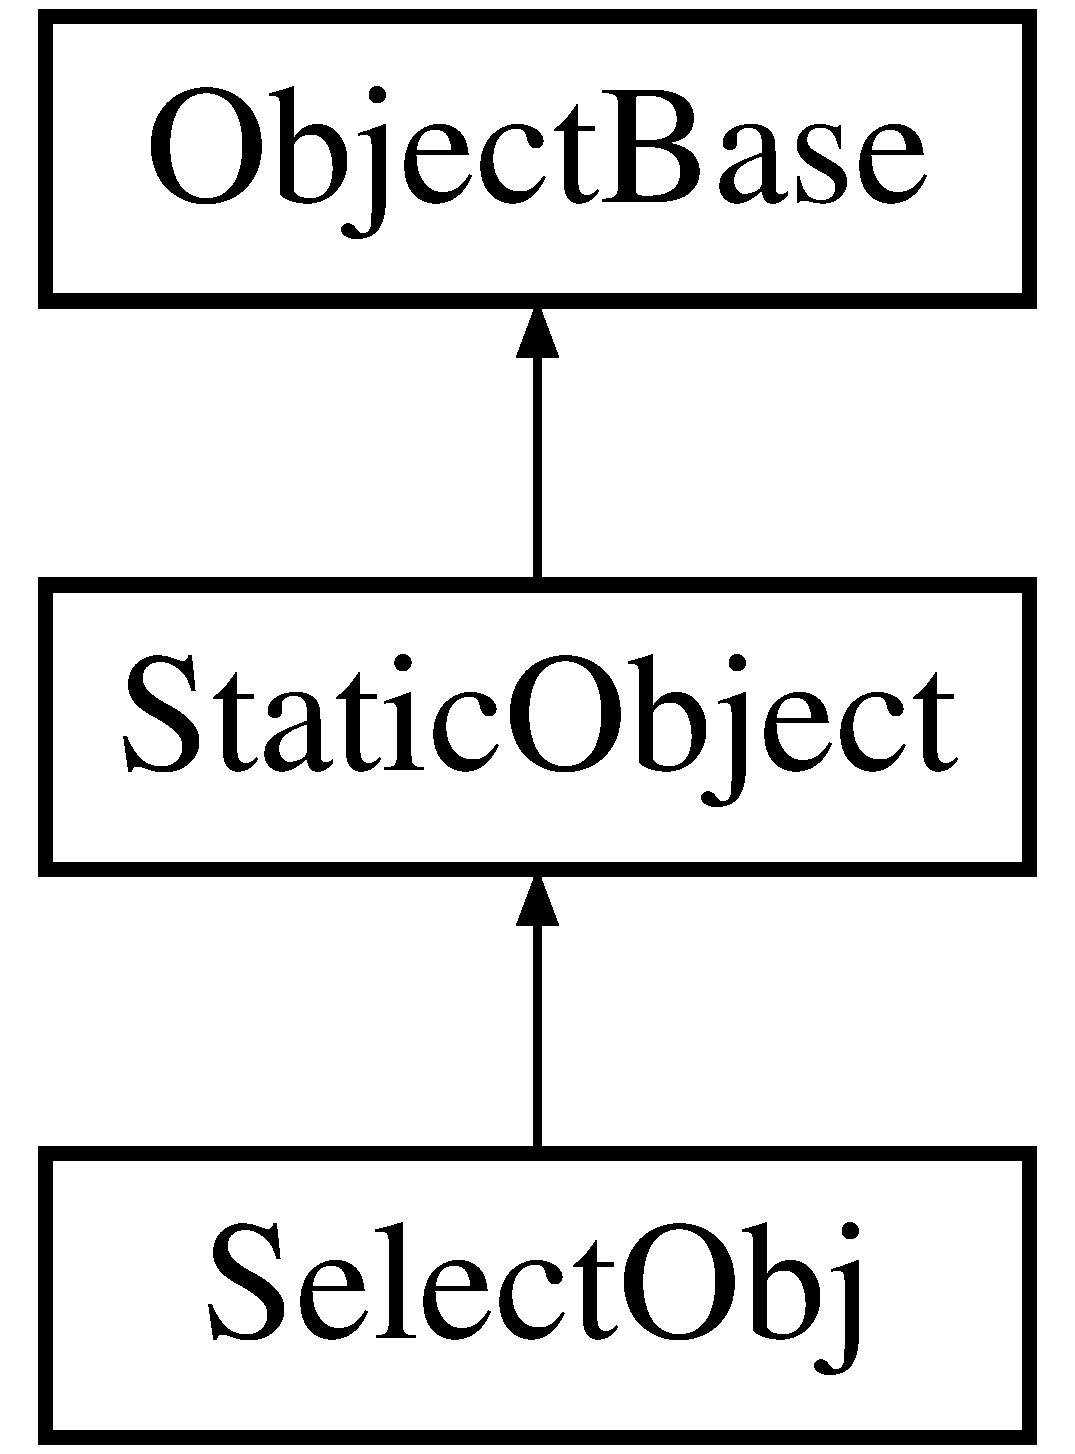
\includegraphics[height=3.000000cm]{class_select_obj}
\end{center}
\end{figure}
\subsection*{公開メンバ関数}
\begin{DoxyCompactItemize}
\item 
void \mbox{\hyperlink{class_select_obj_ad3a5fdc41a9e5753f99bae7ad289888f}{Destroy}} () final
\begin{DoxyCompactList}\small\item\em マップの破棄 \end{DoxyCompactList}\item 
\mbox{\hyperlink{class_select_obj_a38e6ecf0bc37abe109332de38c027853}{Select\+Obj}} ()
\begin{DoxyCompactList}\small\item\em コンストラクタ \end{DoxyCompactList}\item 
\mbox{\hyperlink{class_select_obj_ab62679ab8ef5831c5389fdb234b37188}{Select\+Obj}} (const \mbox{\hyperlink{class_select_obj}{Select\+Obj}} \&m)
\begin{DoxyCompactList}\small\item\em コピーコンストラクタ \end{DoxyCompactList}\item 
\mbox{\hyperlink{class_select_obj_a5d1e7d1696dfdef2eadf25cb4166f2ef}{Select\+Obj}} (\mbox{\hyperlink{class_select_obj}{Select\+Obj}} \&\&m) noexcept
\begin{DoxyCompactList}\small\item\em ムーブコンストラクタ \end{DoxyCompactList}\item 
\mbox{\hyperlink{class_select_obj}{Select\+Obj}} \& \mbox{\hyperlink{class_select_obj_a6faf6b5fed9a6a61f24d1c91e009d0c7}{operator=}} (const \mbox{\hyperlink{class_select_obj}{Select\+Obj}} \&other)
\begin{DoxyCompactList}\small\item\em コピー代入演算子 \end{DoxyCompactList}\item 
\mbox{\hyperlink{class_select_obj}{Select\+Obj}} \& \mbox{\hyperlink{class_select_obj_a31f75f0dc6f8fb01f577bc8e5d4099f8}{operator=}} (\mbox{\hyperlink{class_select_obj}{Select\+Obj}} \&\&other) noexcept
\begin{DoxyCompactList}\small\item\em ムーブ代入演算子 \end{DoxyCompactList}\item 
void \mbox{\hyperlink{class_select_obj_a497ff683aefe9bf77201eee1e3948e15}{Collision}} (\mbox{\hyperlink{class_object_base}{Object\+Base}} $\ast$, \mbox{\hyperlink{common_8h_ae148fff5818e9444b4ab2288829559bf}{Vec2}}) final
\begin{DoxyCompactList}\small\item\em マップが当たってるときに実行する関数 \end{DoxyCompactList}\item 
\mbox{\hyperlink{class_select_obj_a091e4be751b4f828d0780acdd493fa71}{$\sim$\+Select\+Obj}} ()
\begin{DoxyCompactList}\small\item\em デストラクタ \end{DoxyCompactList}\end{DoxyCompactItemize}
\subsection*{公開変数類}
\begin{DoxyCompactItemize}
\item 
bool \mbox{\hyperlink{class_select_obj_a7678b8b51a55e9dcd2b8a003d54c08f5}{collision\+\_\+weapon}} = false
\item 
bool \mbox{\hyperlink{class_select_obj_ab3471f76e003f613f38d396ad42a7860}{another\+\_\+obj\+\_\+collision}} = false
\end{DoxyCompactItemize}
\subsection*{限定公開メンバ関数}
\begin{DoxyCompactItemize}
\item 
void \mbox{\hyperlink{class_select_obj_a09c9e1a54f4605eda5bb6e18887c2654}{Init\+Process}} () final
\begin{DoxyCompactList}\small\item\em 初期化 \end{DoxyCompactList}\item 
void \mbox{\hyperlink{class_select_obj_a4788d957629f0b69dc78166f09f949bb}{Update\+Process}} () final
\begin{DoxyCompactList}\small\item\em マップの更新 \end{DoxyCompactList}\end{DoxyCompactItemize}
\subsection*{その他の継承メンバ}


\subsection{構築子と解体子}
\mbox{\Hypertarget{class_select_obj_a38e6ecf0bc37abe109332de38c027853}\label{class_select_obj_a38e6ecf0bc37abe109332de38c027853}} 
\index{Select\+Obj@{Select\+Obj}!Select\+Obj@{Select\+Obj}}
\index{Select\+Obj@{Select\+Obj}!Select\+Obj@{Select\+Obj}}
\subsubsection{\texorpdfstring{Select\+Obj()}{SelectObj()}\hspace{0.1cm}{\footnotesize\ttfamily [1/3]}}
{\footnotesize\ttfamily Select\+Obj\+::\+Select\+Obj (\begin{DoxyParamCaption}{ }\end{DoxyParamCaption})\hspace{0.3cm}{\ttfamily [inline]}}



コンストラクタ 

\mbox{\Hypertarget{class_select_obj_ab62679ab8ef5831c5389fdb234b37188}\label{class_select_obj_ab62679ab8ef5831c5389fdb234b37188}} 
\index{Select\+Obj@{Select\+Obj}!Select\+Obj@{Select\+Obj}}
\index{Select\+Obj@{Select\+Obj}!Select\+Obj@{Select\+Obj}}
\subsubsection{\texorpdfstring{Select\+Obj()}{SelectObj()}\hspace{0.1cm}{\footnotesize\ttfamily [2/3]}}
{\footnotesize\ttfamily Select\+Obj\+::\+Select\+Obj (\begin{DoxyParamCaption}\item[{const \mbox{\hyperlink{class_select_obj}{Select\+Obj}} \&}]{m }\end{DoxyParamCaption})\hspace{0.3cm}{\ttfamily [inline]}}



コピーコンストラクタ 

\mbox{\Hypertarget{class_select_obj_a5d1e7d1696dfdef2eadf25cb4166f2ef}\label{class_select_obj_a5d1e7d1696dfdef2eadf25cb4166f2ef}} 
\index{Select\+Obj@{Select\+Obj}!Select\+Obj@{Select\+Obj}}
\index{Select\+Obj@{Select\+Obj}!Select\+Obj@{Select\+Obj}}
\subsubsection{\texorpdfstring{Select\+Obj()}{SelectObj()}\hspace{0.1cm}{\footnotesize\ttfamily [3/3]}}
{\footnotesize\ttfamily Select\+Obj\+::\+Select\+Obj (\begin{DoxyParamCaption}\item[{\mbox{\hyperlink{class_select_obj}{Select\+Obj}} \&\&}]{m }\end{DoxyParamCaption})\hspace{0.3cm}{\ttfamily [inline]}, {\ttfamily [noexcept]}}



ムーブコンストラクタ 

\mbox{\Hypertarget{class_select_obj_a091e4be751b4f828d0780acdd493fa71}\label{class_select_obj_a091e4be751b4f828d0780acdd493fa71}} 
\index{Select\+Obj@{Select\+Obj}!````~Select\+Obj@{$\sim$\+Select\+Obj}}
\index{````~Select\+Obj@{$\sim$\+Select\+Obj}!Select\+Obj@{Select\+Obj}}
\subsubsection{\texorpdfstring{$\sim$\+Select\+Obj()}{~SelectObj()}}
{\footnotesize\ttfamily Select\+Obj\+::$\sim$\+Select\+Obj (\begin{DoxyParamCaption}{ }\end{DoxyParamCaption})\hspace{0.3cm}{\ttfamily [inline]}}



デストラクタ 



\subsection{関数詳解}
\mbox{\Hypertarget{class_select_obj_a497ff683aefe9bf77201eee1e3948e15}\label{class_select_obj_a497ff683aefe9bf77201eee1e3948e15}} 
\index{Select\+Obj@{Select\+Obj}!Collision@{Collision}}
\index{Collision@{Collision}!Select\+Obj@{Select\+Obj}}
\subsubsection{\texorpdfstring{Collision()}{Collision()}}
{\footnotesize\ttfamily void Select\+Obj\+::\+Collision (\begin{DoxyParamCaption}\item[{\mbox{\hyperlink{class_object_base}{Object\+Base}} $\ast$}]{obj,  }\item[{\mbox{\hyperlink{common_8h_ae148fff5818e9444b4ab2288829559bf}{Vec2}}}]{ }\end{DoxyParamCaption})\hspace{0.3cm}{\ttfamily [final]}, {\ttfamily [virtual]}}



マップが当たってるときに実行する関数 



\mbox{\hyperlink{class_static_object_a64c8803ff881d578d103413e299dbf7f}{Static\+Object}}を再実装しています。

\mbox{\Hypertarget{class_select_obj_ad3a5fdc41a9e5753f99bae7ad289888f}\label{class_select_obj_ad3a5fdc41a9e5753f99bae7ad289888f}} 
\index{Select\+Obj@{Select\+Obj}!Destroy@{Destroy}}
\index{Destroy@{Destroy}!Select\+Obj@{Select\+Obj}}
\subsubsection{\texorpdfstring{Destroy()}{Destroy()}}
{\footnotesize\ttfamily void Select\+Obj\+::\+Destroy (\begin{DoxyParamCaption}{ }\end{DoxyParamCaption})\hspace{0.3cm}{\ttfamily [final]}, {\ttfamily [virtual]}}



マップの破棄 



\mbox{\hyperlink{class_static_object_a8e9fb321b4f8f12c4bec1bc66853512f}{Static\+Object}}を再実装しています。

\mbox{\Hypertarget{class_select_obj_a09c9e1a54f4605eda5bb6e18887c2654}\label{class_select_obj_a09c9e1a54f4605eda5bb6e18887c2654}} 
\index{Select\+Obj@{Select\+Obj}!Init\+Process@{Init\+Process}}
\index{Init\+Process@{Init\+Process}!Select\+Obj@{Select\+Obj}}
\subsubsection{\texorpdfstring{Init\+Process()}{InitProcess()}}
{\footnotesize\ttfamily void Select\+Obj\+::\+Init\+Process (\begin{DoxyParamCaption}{ }\end{DoxyParamCaption})\hspace{0.3cm}{\ttfamily [final]}, {\ttfamily [protected]}, {\ttfamily [virtual]}}



初期化 



\mbox{\hyperlink{class_static_object_afa0709f50495338a23c1140062a567af}{Static\+Object}}を再実装しています。

\mbox{\Hypertarget{class_select_obj_a6faf6b5fed9a6a61f24d1c91e009d0c7}\label{class_select_obj_a6faf6b5fed9a6a61f24d1c91e009d0c7}} 
\index{Select\+Obj@{Select\+Obj}!operator=@{operator=}}
\index{operator=@{operator=}!Select\+Obj@{Select\+Obj}}
\subsubsection{\texorpdfstring{operator=()}{operator=()}\hspace{0.1cm}{\footnotesize\ttfamily [1/2]}}
{\footnotesize\ttfamily \mbox{\hyperlink{class_select_obj}{Select\+Obj}}\& Select\+Obj\+::operator= (\begin{DoxyParamCaption}\item[{const \mbox{\hyperlink{class_select_obj}{Select\+Obj}} \&}]{other }\end{DoxyParamCaption})\hspace{0.3cm}{\ttfamily [inline]}}



コピー代入演算子 

\mbox{\Hypertarget{class_select_obj_a31f75f0dc6f8fb01f577bc8e5d4099f8}\label{class_select_obj_a31f75f0dc6f8fb01f577bc8e5d4099f8}} 
\index{Select\+Obj@{Select\+Obj}!operator=@{operator=}}
\index{operator=@{operator=}!Select\+Obj@{Select\+Obj}}
\subsubsection{\texorpdfstring{operator=()}{operator=()}\hspace{0.1cm}{\footnotesize\ttfamily [2/2]}}
{\footnotesize\ttfamily \mbox{\hyperlink{class_select_obj}{Select\+Obj}}\& Select\+Obj\+::operator= (\begin{DoxyParamCaption}\item[{\mbox{\hyperlink{class_select_obj}{Select\+Obj}} \&\&}]{other }\end{DoxyParamCaption})\hspace{0.3cm}{\ttfamily [inline]}, {\ttfamily [noexcept]}}



ムーブ代入演算子 

\mbox{\Hypertarget{class_select_obj_a4788d957629f0b69dc78166f09f949bb}\label{class_select_obj_a4788d957629f0b69dc78166f09f949bb}} 
\index{Select\+Obj@{Select\+Obj}!Update\+Process@{Update\+Process}}
\index{Update\+Process@{Update\+Process}!Select\+Obj@{Select\+Obj}}
\subsubsection{\texorpdfstring{Update\+Process()}{UpdateProcess()}}
{\footnotesize\ttfamily void Select\+Obj\+::\+Update\+Process (\begin{DoxyParamCaption}{ }\end{DoxyParamCaption})\hspace{0.3cm}{\ttfamily [final]}, {\ttfamily [protected]}, {\ttfamily [virtual]}}



マップの更新 



\mbox{\hyperlink{class_static_object_a7fa678c3c4032bb6e9417f93a8bb895c}{Static\+Object}}を再実装しています。



\subsection{メンバ詳解}
\mbox{\Hypertarget{class_select_obj_ab3471f76e003f613f38d396ad42a7860}\label{class_select_obj_ab3471f76e003f613f38d396ad42a7860}} 
\index{Select\+Obj@{Select\+Obj}!another\+\_\+obj\+\_\+collision@{another\+\_\+obj\+\_\+collision}}
\index{another\+\_\+obj\+\_\+collision@{another\+\_\+obj\+\_\+collision}!Select\+Obj@{Select\+Obj}}
\subsubsection{\texorpdfstring{another\+\_\+obj\+\_\+collision}{another\_obj\_collision}}
{\footnotesize\ttfamily bool Select\+Obj\+::another\+\_\+obj\+\_\+collision = false}

\mbox{\Hypertarget{class_select_obj_a7678b8b51a55e9dcd2b8a003d54c08f5}\label{class_select_obj_a7678b8b51a55e9dcd2b8a003d54c08f5}} 
\index{Select\+Obj@{Select\+Obj}!collision\+\_\+weapon@{collision\+\_\+weapon}}
\index{collision\+\_\+weapon@{collision\+\_\+weapon}!Select\+Obj@{Select\+Obj}}
\subsubsection{\texorpdfstring{collision\+\_\+weapon}{collision\_weapon}}
{\footnotesize\ttfamily bool Select\+Obj\+::collision\+\_\+weapon = false}



このクラス詳解は次のファイルから抽出されました\+:\begin{DoxyCompactItemize}
\item 
C\+:/\+Users/tokir/\+Documents/\+Git\+Hub/\+Weapon\+Merchant\+Adventure/src/src/object/select/\mbox{\hyperlink{select__object_8h}{select\+\_\+object.\+h}}\item 
C\+:/\+Users/tokir/\+Documents/\+Git\+Hub/\+Weapon\+Merchant\+Adventure/src/src/object/select/\mbox{\hyperlink{select__object_8cpp}{select\+\_\+object.\+cpp}}\end{DoxyCompactItemize}

\hypertarget{class_select_scene}{}\section{Select\+Scene クラス}
\label{class_select_scene}\index{Select\+Scene@{Select\+Scene}}


セレクトシーンクラス  




{\ttfamily \#include $<$select\+\_\+scene.\+h$>$}

Select\+Scene の継承関係図\begin{figure}[H]
\begin{center}
\leavevmode
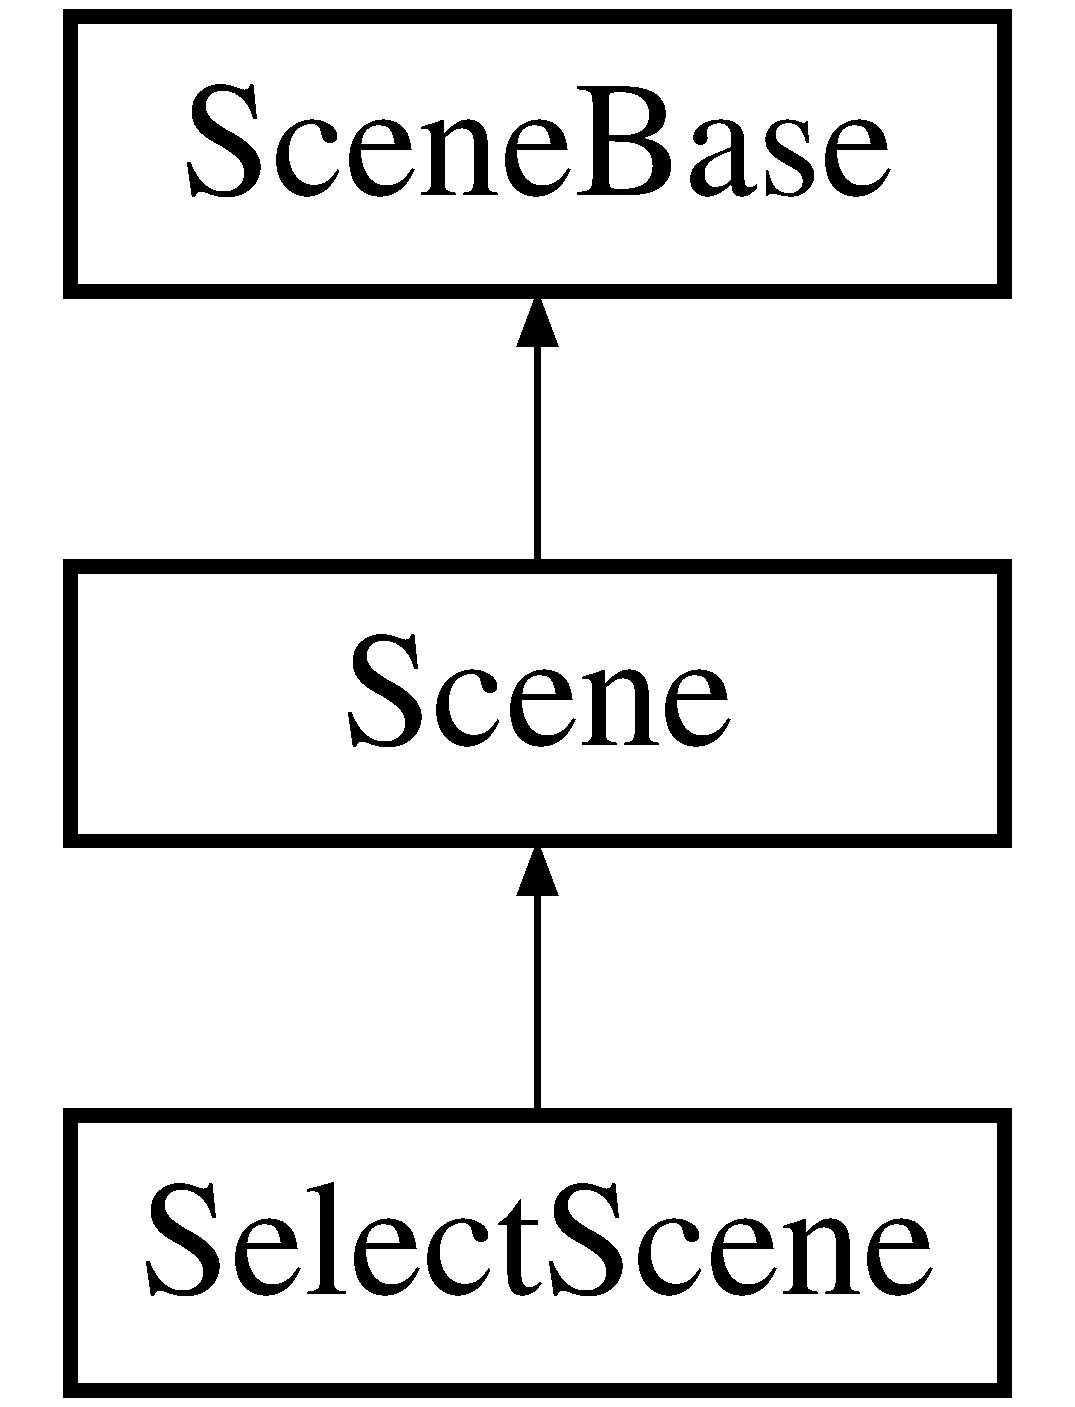
\includegraphics[height=3.000000cm]{class_select_scene}
\end{center}
\end{figure}
\subsection*{公開メンバ関数}
\begin{DoxyCompactItemize}
\item 
void \mbox{\hyperlink{class_select_scene_a20b3a902b5521d7494ed353731b3065d}{Init}} () final
\begin{DoxyCompactList}\small\item\em セレクトシーンの初期化 \end{DoxyCompactList}\item 
std\+::shared\+\_\+ptr$<$ \mbox{\hyperlink{class_scene}{Scene}} $>$ \mbox{\hyperlink{class_select_scene_a0cef696ddf74155e061cc5f9f2e06419}{Update}} (std\+::shared\+\_\+ptr$<$ \mbox{\hyperlink{class_scene}{Scene}} $>$ \&) final
\begin{DoxyCompactList}\small\item\em セレクトシーンの更新 \end{DoxyCompactList}\item 
void \mbox{\hyperlink{class_select_scene_a85445536ad84d5232c724ecb7d48b8aa}{Render}} () final
\begin{DoxyCompactList}\small\item\em セレクトシーンの描画 \end{DoxyCompactList}\item 
void \mbox{\hyperlink{class_select_scene_a938293516c0e1ae5bb09dbab81bc78d9}{Destroy}} () final
\begin{DoxyCompactList}\small\item\em セレクトシーンの破棄 \end{DoxyCompactList}\item 
void \mbox{\hyperlink{class_select_scene_a546190bc143f6d7a3055935f97b55596}{Exit\+Fade\+Update}} () final
\begin{DoxyCompactList}\small\item\em フェード中の更新 \end{DoxyCompactList}\end{DoxyCompactItemize}


\subsection{詳解}
セレクトシーンクラス 

\subsection{関数詳解}
\mbox{\Hypertarget{class_select_scene_a938293516c0e1ae5bb09dbab81bc78d9}\label{class_select_scene_a938293516c0e1ae5bb09dbab81bc78d9}} 
\index{Select\+Scene@{Select\+Scene}!Destroy@{Destroy}}
\index{Destroy@{Destroy}!Select\+Scene@{Select\+Scene}}
\subsubsection{\texorpdfstring{Destroy()}{Destroy()}}
{\footnotesize\ttfamily void Select\+Scene\+::\+Destroy (\begin{DoxyParamCaption}{ }\end{DoxyParamCaption})\hspace{0.3cm}{\ttfamily [final]}, {\ttfamily [virtual]}}



セレクトシーンの破棄 



\mbox{\hyperlink{class_scene_base_a7c5b54020bc519b4dadfe9770d6b27f7}{Scene\+Base}}を実装しています。

\mbox{\Hypertarget{class_select_scene_a546190bc143f6d7a3055935f97b55596}\label{class_select_scene_a546190bc143f6d7a3055935f97b55596}} 
\index{Select\+Scene@{Select\+Scene}!Exit\+Fade\+Update@{Exit\+Fade\+Update}}
\index{Exit\+Fade\+Update@{Exit\+Fade\+Update}!Select\+Scene@{Select\+Scene}}
\subsubsection{\texorpdfstring{Exit\+Fade\+Update()}{ExitFadeUpdate()}}
{\footnotesize\ttfamily void Select\+Scene\+::\+Exit\+Fade\+Update (\begin{DoxyParamCaption}{ }\end{DoxyParamCaption})\hspace{0.3cm}{\ttfamily [final]}, {\ttfamily [virtual]}}



フェード中の更新 



\mbox{\hyperlink{class_scene_ad19a449c6ed452823dae14183689570c}{Scene}}を再実装しています。

\mbox{\Hypertarget{class_select_scene_a20b3a902b5521d7494ed353731b3065d}\label{class_select_scene_a20b3a902b5521d7494ed353731b3065d}} 
\index{Select\+Scene@{Select\+Scene}!Init@{Init}}
\index{Init@{Init}!Select\+Scene@{Select\+Scene}}
\subsubsection{\texorpdfstring{Init()}{Init()}}
{\footnotesize\ttfamily void Select\+Scene\+::\+Init (\begin{DoxyParamCaption}{ }\end{DoxyParamCaption})\hspace{0.3cm}{\ttfamily [final]}, {\ttfamily [virtual]}}



セレクトシーンの初期化 



\mbox{\hyperlink{class_scene_base_a24d7db43c819924dc8b07b436f6d3148}{Scene\+Base}}を実装しています。

\mbox{\Hypertarget{class_select_scene_a85445536ad84d5232c724ecb7d48b8aa}\label{class_select_scene_a85445536ad84d5232c724ecb7d48b8aa}} 
\index{Select\+Scene@{Select\+Scene}!Render@{Render}}
\index{Render@{Render}!Select\+Scene@{Select\+Scene}}
\subsubsection{\texorpdfstring{Render()}{Render()}}
{\footnotesize\ttfamily void Select\+Scene\+::\+Render (\begin{DoxyParamCaption}{ }\end{DoxyParamCaption})\hspace{0.3cm}{\ttfamily [final]}, {\ttfamily [virtual]}}



セレクトシーンの描画 



\mbox{\hyperlink{class_scene_base_ad981674ce731ea267f398e889bbb9dc3}{Scene\+Base}}を実装しています。

\mbox{\Hypertarget{class_select_scene_a0cef696ddf74155e061cc5f9f2e06419}\label{class_select_scene_a0cef696ddf74155e061cc5f9f2e06419}} 
\index{Select\+Scene@{Select\+Scene}!Update@{Update}}
\index{Update@{Update}!Select\+Scene@{Select\+Scene}}
\subsubsection{\texorpdfstring{Update()}{Update()}}
{\footnotesize\ttfamily std\+::shared\+\_\+ptr$<$ \mbox{\hyperlink{class_scene}{Scene}} $>$ Select\+Scene\+::\+Update (\begin{DoxyParamCaption}\item[{std\+::shared\+\_\+ptr$<$ \mbox{\hyperlink{class_scene}{Scene}} $>$ \&}]{scene }\end{DoxyParamCaption})\hspace{0.3cm}{\ttfamily [final]}, {\ttfamily [virtual]}}



セレクトシーンの更新 

\begin{DoxyReturn}{戻り値}
std\+::shared\+\_\+ptr$<$\+Scene$>$ シーンが変わるなら次のシーンのstd\+::shared\+\_\+ptr$<$\+Scene$>$を返す 
\end{DoxyReturn}


\mbox{\hyperlink{class_scene_ab71ee5f19764b90c87b4574aa1cb1d25}{Scene}}を実装しています。



このクラス詳解は次のファイルから抽出されました\+:\begin{DoxyCompactItemize}
\item 
C\+:/\+Users/tokir/\+Documents/\+Git\+Hub/\+Weapon\+Merchant\+Adventure/src/src/scene/main/select/\mbox{\hyperlink{select__scene_8h}{select\+\_\+scene.\+h}}\item 
C\+:/\+Users/tokir/\+Documents/\+Git\+Hub/\+Weapon\+Merchant\+Adventure/src/src/scene/main/select/\mbox{\hyperlink{select__scene_8cpp}{select\+\_\+scene.\+cpp}}\end{DoxyCompactItemize}

\hypertarget{class_shader}{}\section{Shader クラス}
\label{class_shader}\index{Shader@{Shader}}


{\ttfamily \#include $<$shader.\+h$>$}

\subsection*{公開メンバ関数}
\begin{DoxyCompactItemize}
\item 
H\+R\+E\+S\+U\+LT \mbox{\hyperlink{class_shader_a357cc3cef65b5c73f680bdebf0f08015}{load\+\_\+shader}} (const std\+::string \&key, const W\+C\+H\+AR $\ast$vertex\+\_\+path, const W\+C\+H\+AR $\ast$pixel\+\_\+path, \mbox{\hyperlink{common_8h_ab7d7d9064a34dd725663b1dbee652aca}{Com\+Ptr}}$<$ I\+D3\+D\+Blob $>$ \&v\+\_\+blob, \mbox{\hyperlink{common_8h_ab7d7d9064a34dd725663b1dbee652aca}{Com\+Ptr}}$<$ I\+D3\+D\+Blob $>$ \&p\+\_\+blob)
\item 
void \mbox{\hyperlink{class_shader_a0494397acc115e563051c5adfa3ea6db}{set\+\_\+shader}} ()
\end{DoxyCompactItemize}


\subsection{関数詳解}
\mbox{\Hypertarget{class_shader_a357cc3cef65b5c73f680bdebf0f08015}\label{class_shader_a357cc3cef65b5c73f680bdebf0f08015}} 
\index{Shader@{Shader}!load\+\_\+shader@{load\+\_\+shader}}
\index{load\+\_\+shader@{load\+\_\+shader}!Shader@{Shader}}
\subsubsection{\texorpdfstring{load\+\_\+shader()}{load\_shader()}}
{\footnotesize\ttfamily H\+R\+E\+S\+U\+LT Shader\+::load\+\_\+shader (\begin{DoxyParamCaption}\item[{const std\+::string \&}]{key,  }\item[{const W\+C\+H\+AR $\ast$}]{vertex\+\_\+path,  }\item[{const W\+C\+H\+AR $\ast$}]{pixel\+\_\+path,  }\item[{\mbox{\hyperlink{common_8h_ab7d7d9064a34dd725663b1dbee652aca}{Com\+Ptr}}$<$ I\+D3\+D\+Blob $>$ \&}]{v\+\_\+blob,  }\item[{\mbox{\hyperlink{common_8h_ab7d7d9064a34dd725663b1dbee652aca}{Com\+Ptr}}$<$ I\+D3\+D\+Blob $>$ \&}]{p\+\_\+blob }\end{DoxyParamCaption})\hspace{0.3cm}{\ttfamily [inline]}}

\mbox{\Hypertarget{class_shader_a0494397acc115e563051c5adfa3ea6db}\label{class_shader_a0494397acc115e563051c5adfa3ea6db}} 
\index{Shader@{Shader}!set\+\_\+shader@{set\+\_\+shader}}
\index{set\+\_\+shader@{set\+\_\+shader}!Shader@{Shader}}
\subsubsection{\texorpdfstring{set\+\_\+shader()}{set\_shader()}}
{\footnotesize\ttfamily void Shader\+::set\+\_\+shader (\begin{DoxyParamCaption}{ }\end{DoxyParamCaption})\hspace{0.3cm}{\ttfamily [inline]}}



このクラス詳解は次のファイルから抽出されました\+:\begin{DoxyCompactItemize}
\item 
C\+:/\+Users/tokir/\+Documents/\+Git\+Hub/\+Weapon\+Merchant\+Adventure/src/src/shader/\mbox{\hyperlink{shader_8h}{shader.\+h}}\end{DoxyCompactItemize}

\hypertarget{class_shader_manager}{}\section{Shader\+Manager クラス}
\label{class_shader_manager}\index{Shader\+Manager@{Shader\+Manager}}


{\ttfamily \#include $<$shader\+\_\+manager.\+h$>$}

Shader\+Manager の継承関係図\begin{figure}[H]
\begin{center}
\leavevmode
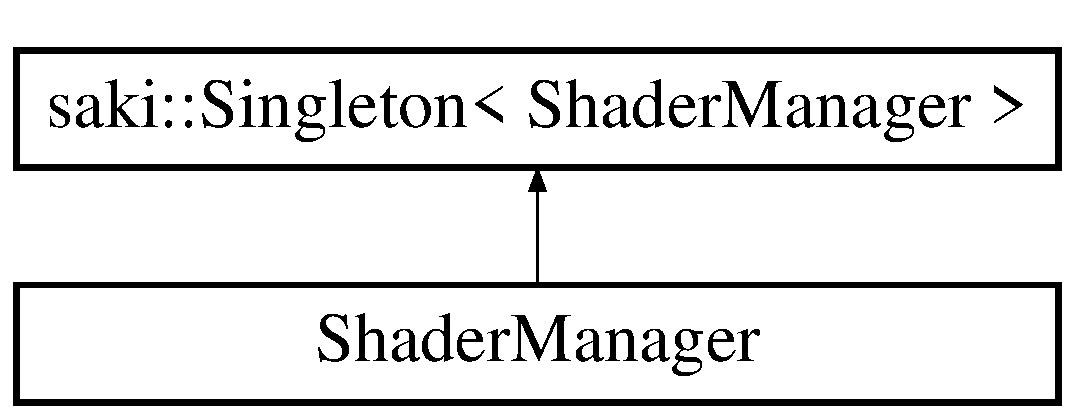
\includegraphics[height=2.000000cm]{class_shader_manager}
\end{center}
\end{figure}
\subsection*{フレンド}
\begin{DoxyCompactItemize}
\item 
class \mbox{\hyperlink{class_shader_manager_a03c2d524ace9ade9c3f55b43c99bcea1}{Shader}}
\end{DoxyCompactItemize}
\subsection*{その他の継承メンバ}


\subsection{フレンドと関連関数の詳解}
\mbox{\Hypertarget{class_shader_manager_a03c2d524ace9ade9c3f55b43c99bcea1}\label{class_shader_manager_a03c2d524ace9ade9c3f55b43c99bcea1}} 
\index{Shader\+Manager@{Shader\+Manager}!Shader@{Shader}}
\index{Shader@{Shader}!Shader\+Manager@{Shader\+Manager}}
\subsubsection{\texorpdfstring{Shader}{Shader}}
{\footnotesize\ttfamily friend class \mbox{\hyperlink{class_shader}{Shader}}\hspace{0.3cm}{\ttfamily [friend]}}



このクラス詳解は次のファイルから抽出されました\+:\begin{DoxyCompactItemize}
\item 
C\+:/\+Users/tokir/\+Documents/\+Git\+Hub/\+Weapon\+Merchant\+Adventure/src/src/shader/manager/\mbox{\hyperlink{shader__manager_8h}{shader\+\_\+manager.\+h}}\item 
C\+:/\+Users/tokir/\+Documents/\+Git\+Hub/\+Weapon\+Merchant\+Adventure/src/src/shader/manager/\mbox{\hyperlink{shader__manager_8cpp}{shader\+\_\+manager.\+cpp}}\end{DoxyCompactItemize}

\hypertarget{classsaki_1_1_singleton}{}\section{saki\+:\+:Singleton$<$ T $>$ クラステンプレート}
\label{classsaki_1_1_singleton}\index{saki\+::\+Singleton$<$ T $>$@{saki\+::\+Singleton$<$ T $>$}}


継承するとシングルトンクラスになる  




{\ttfamily \#include $<$singleton.\+h$>$}

\subsection*{公開メンバ関数}
\begin{DoxyCompactItemize}
\item 
virtual \mbox{\hyperlink{classsaki_1_1_singleton_a3ff92ba5c83fba36d539cfa16d35599a}{$\sim$\+Singleton}} ()
\end{DoxyCompactItemize}
\subsection*{静的公開メンバ関数}
\begin{DoxyCompactItemize}
\item 
static std\+::unique\+\_\+ptr$<$ T $>$ \& \mbox{\hyperlink{classsaki_1_1_singleton_a198911b1e5a72914511ffd6f50e4da2f}{getinstance}} ()
\begin{DoxyCompactList}\small\item\em インスタンスを取得 \end{DoxyCompactList}\end{DoxyCompactItemize}
\subsection*{限定公開メンバ関数}
\begin{DoxyCompactItemize}
\item 
\mbox{\hyperlink{classsaki_1_1_singleton_a1cd9f69783e3c0c83db851edc061bb7f}{Singleton}} ()
\end{DoxyCompactItemize}


\subsection{詳解}
\subsubsection*{template$<$typename T$>$\newline
class saki\+::\+Singleton$<$ T $>$}

継承するとシングルトンクラスになる 

\subsection{構築子と解体子}
\mbox{\Hypertarget{classsaki_1_1_singleton_a3ff92ba5c83fba36d539cfa16d35599a}\label{classsaki_1_1_singleton_a3ff92ba5c83fba36d539cfa16d35599a}} 
\index{saki\+::\+Singleton@{saki\+::\+Singleton}!````~Singleton@{$\sim$\+Singleton}}
\index{````~Singleton@{$\sim$\+Singleton}!saki\+::\+Singleton@{saki\+::\+Singleton}}
\subsubsection{\texorpdfstring{$\sim$\+Singleton()}{~Singleton()}}
{\footnotesize\ttfamily template$<$typename T$>$ \\
virtual \mbox{\hyperlink{classsaki_1_1_singleton}{saki\+::\+Singleton}}$<$ T $>$\+::$\sim$\mbox{\hyperlink{classsaki_1_1_singleton}{Singleton}} (\begin{DoxyParamCaption}{ }\end{DoxyParamCaption})\hspace{0.3cm}{\ttfamily [inline]}, {\ttfamily [virtual]}}

\mbox{\Hypertarget{classsaki_1_1_singleton_a1cd9f69783e3c0c83db851edc061bb7f}\label{classsaki_1_1_singleton_a1cd9f69783e3c0c83db851edc061bb7f}} 
\index{saki\+::\+Singleton@{saki\+::\+Singleton}!Singleton@{Singleton}}
\index{Singleton@{Singleton}!saki\+::\+Singleton@{saki\+::\+Singleton}}
\subsubsection{\texorpdfstring{Singleton()}{Singleton()}}
{\footnotesize\ttfamily template$<$typename T$>$ \\
\mbox{\hyperlink{classsaki_1_1_singleton}{saki\+::\+Singleton}}$<$ T $>$\+::\mbox{\hyperlink{classsaki_1_1_singleton}{Singleton}} (\begin{DoxyParamCaption}{ }\end{DoxyParamCaption})\hspace{0.3cm}{\ttfamily [inline]}, {\ttfamily [protected]}}



\subsection{関数詳解}
\mbox{\Hypertarget{classsaki_1_1_singleton_a198911b1e5a72914511ffd6f50e4da2f}\label{classsaki_1_1_singleton_a198911b1e5a72914511ffd6f50e4da2f}} 
\index{saki\+::\+Singleton@{saki\+::\+Singleton}!getinstance@{getinstance}}
\index{getinstance@{getinstance}!saki\+::\+Singleton@{saki\+::\+Singleton}}
\subsubsection{\texorpdfstring{getinstance()}{getinstance()}}
{\footnotesize\ttfamily template$<$typename T$>$ \\
static std\+::unique\+\_\+ptr$<$T$>$\& \mbox{\hyperlink{classsaki_1_1_singleton}{saki\+::\+Singleton}}$<$ T $>$\+::getinstance (\begin{DoxyParamCaption}{ }\end{DoxyParamCaption})\hspace{0.3cm}{\ttfamily [inline]}, {\ttfamily [static]}}



インスタンスを取得 

\begin{DoxyReturn}{戻り値}
std\+::unique\+\_\+ptr$<$\+T$>$ インスタンスを返す 
\end{DoxyReturn}


このクラス詳解は次のファイルから抽出されました\+:\begin{DoxyCompactItemize}
\item 
C\+:/\+Users/tokir/\+Documents/\+Git\+Hub/\+Weapon\+Merchant\+Adventure/src/lib/saki/singleton/\mbox{\hyperlink{singleton_8h}{singleton.\+h}}\end{DoxyCompactItemize}

\hypertarget{class_sound}{}\section{Sound クラス}
\label{class_sound}\index{Sound@{Sound}}


 個々のサウンドクラス  




{\ttfamily \#include $<$sound.\+h$>$}

\subsection*{公開メンバ関数}
\begin{DoxyCompactItemize}
\item 
void \mbox{\hyperlink{class_sound_a3c8007c8e52bf541fc81adfa4b340b0f}{Init}} (W\+C\+H\+AR $\ast$, bool, bool)
\begin{DoxyCompactList}\small\item\em サウンドの初期化 \end{DoxyCompactList}\item 
void \mbox{\hyperlink{class_sound_ae021b518e93d7d8c6f3ea951cd4b98d8}{Start}} ()
\item 
void \mbox{\hyperlink{class_sound_a188de6836d531813da378464e392e813}{Stop}} ()
\item 
void \mbox{\hyperlink{class_sound_a4e199b4346519a4977fe94998c4a77e7}{Pause}} ()
\item 
void \mbox{\hyperlink{class_sound_a993eee69f61611ca1b4621ea0952e2c8}{Set\+Volume}} (float vol)
\item 
void \mbox{\hyperlink{class_sound_a06b9680efb2b6b41b52d9f25ac0264f1}{Set\+Pitch}} (float pit)
\item 
void \mbox{\hyperlink{class_sound_a1b066e78405656b1475849139ca24dce}{Set\+Pan}} (float pan)
\item 
\mbox{\hyperlink{class_sound_a0907389078bf740be2a5763366ad3376}{$\sim$\+Sound}} ()
\begin{DoxyCompactList}\small\item\em デストラクタ \end{DoxyCompactList}\item 
std\+::unique\+\_\+ptr$<$ Direct\+X\+::\+Sound\+Effect\+Instance $>$ \& \mbox{\hyperlink{class_sound_a0d79b20f421c0020c53b08c05b6df25b}{operator()}} ()
\end{DoxyCompactItemize}


\subsection{詳解}
 個々のサウンドクラス 

\subsection{構築子と解体子}
\mbox{\Hypertarget{class_sound_a0907389078bf740be2a5763366ad3376}\label{class_sound_a0907389078bf740be2a5763366ad3376}} 
\index{Sound@{Sound}!````~Sound@{$\sim$\+Sound}}
\index{````~Sound@{$\sim$\+Sound}!Sound@{Sound}}
\subsubsection{\texorpdfstring{$\sim$\+Sound()}{~Sound()}}
{\footnotesize\ttfamily Sound\+::$\sim$\+Sound (\begin{DoxyParamCaption}{ }\end{DoxyParamCaption})}



デストラクタ 



\subsection{関数詳解}
\mbox{\Hypertarget{class_sound_a3c8007c8e52bf541fc81adfa4b340b0f}\label{class_sound_a3c8007c8e52bf541fc81adfa4b340b0f}} 
\index{Sound@{Sound}!Init@{Init}}
\index{Init@{Init}!Sound@{Sound}}
\subsubsection{\texorpdfstring{Init()}{Init()}}
{\footnotesize\ttfamily void Sound\+::\+Init (\begin{DoxyParamCaption}\item[{W\+C\+H\+AR $\ast$}]{path,  }\item[{bool}]{loop,  }\item[{bool}]{awake }\end{DoxyParamCaption})}



サウンドの初期化 


\begin{DoxyParams}{引数}
{\em path} & サウンドのパス \\
\hline
{\em loop} & ループするかどうか \\
\hline
{\em awake} & 初期化した瞬間から再生するかどうか \\
\hline
\end{DoxyParams}
\mbox{\Hypertarget{class_sound_a0d79b20f421c0020c53b08c05b6df25b}\label{class_sound_a0d79b20f421c0020c53b08c05b6df25b}} 
\index{Sound@{Sound}!operator()@{operator()}}
\index{operator()@{operator()}!Sound@{Sound}}
\subsubsection{\texorpdfstring{operator()()}{operator()()}}
{\footnotesize\ttfamily std\+::unique\+\_\+ptr$<$Direct\+X\+::\+Sound\+Effect\+Instance$>$\& Sound\+::operator() (\begin{DoxyParamCaption}{ }\end{DoxyParamCaption})\hspace{0.3cm}{\ttfamily [inline]}}

\mbox{\Hypertarget{class_sound_a4e199b4346519a4977fe94998c4a77e7}\label{class_sound_a4e199b4346519a4977fe94998c4a77e7}} 
\index{Sound@{Sound}!Pause@{Pause}}
\index{Pause@{Pause}!Sound@{Sound}}
\subsubsection{\texorpdfstring{Pause()}{Pause()}}
{\footnotesize\ttfamily void Sound\+::\+Pause (\begin{DoxyParamCaption}{ }\end{DoxyParamCaption})\hspace{0.3cm}{\ttfamily [inline]}}

\mbox{\Hypertarget{class_sound_a1b066e78405656b1475849139ca24dce}\label{class_sound_a1b066e78405656b1475849139ca24dce}} 
\index{Sound@{Sound}!Set\+Pan@{Set\+Pan}}
\index{Set\+Pan@{Set\+Pan}!Sound@{Sound}}
\subsubsection{\texorpdfstring{Set\+Pan()}{SetPan()}}
{\footnotesize\ttfamily void Sound\+::\+Set\+Pan (\begin{DoxyParamCaption}\item[{float}]{pan }\end{DoxyParamCaption})\hspace{0.3cm}{\ttfamily [inline]}}

\mbox{\Hypertarget{class_sound_a06b9680efb2b6b41b52d9f25ac0264f1}\label{class_sound_a06b9680efb2b6b41b52d9f25ac0264f1}} 
\index{Sound@{Sound}!Set\+Pitch@{Set\+Pitch}}
\index{Set\+Pitch@{Set\+Pitch}!Sound@{Sound}}
\subsubsection{\texorpdfstring{Set\+Pitch()}{SetPitch()}}
{\footnotesize\ttfamily void Sound\+::\+Set\+Pitch (\begin{DoxyParamCaption}\item[{float}]{pit }\end{DoxyParamCaption})\hspace{0.3cm}{\ttfamily [inline]}}

\mbox{\Hypertarget{class_sound_a993eee69f61611ca1b4621ea0952e2c8}\label{class_sound_a993eee69f61611ca1b4621ea0952e2c8}} 
\index{Sound@{Sound}!Set\+Volume@{Set\+Volume}}
\index{Set\+Volume@{Set\+Volume}!Sound@{Sound}}
\subsubsection{\texorpdfstring{Set\+Volume()}{SetVolume()}}
{\footnotesize\ttfamily void Sound\+::\+Set\+Volume (\begin{DoxyParamCaption}\item[{float}]{vol }\end{DoxyParamCaption})\hspace{0.3cm}{\ttfamily [inline]}}

\mbox{\Hypertarget{class_sound_ae021b518e93d7d8c6f3ea951cd4b98d8}\label{class_sound_ae021b518e93d7d8c6f3ea951cd4b98d8}} 
\index{Sound@{Sound}!Start@{Start}}
\index{Start@{Start}!Sound@{Sound}}
\subsubsection{\texorpdfstring{Start()}{Start()}}
{\footnotesize\ttfamily void Sound\+::\+Start (\begin{DoxyParamCaption}{ }\end{DoxyParamCaption})\hspace{0.3cm}{\ttfamily [inline]}}

\mbox{\Hypertarget{class_sound_a188de6836d531813da378464e392e813}\label{class_sound_a188de6836d531813da378464e392e813}} 
\index{Sound@{Sound}!Stop@{Stop}}
\index{Stop@{Stop}!Sound@{Sound}}
\subsubsection{\texorpdfstring{Stop()}{Stop()}}
{\footnotesize\ttfamily void Sound\+::\+Stop (\begin{DoxyParamCaption}{ }\end{DoxyParamCaption})\hspace{0.3cm}{\ttfamily [inline]}}



このクラス詳解は次のファイルから抽出されました\+:\begin{DoxyCompactItemize}
\item 
C\+:/\+Users/tokir/\+Documents/\+Git\+Hub/\+Weapon\+Merchant\+Adventure/src/sound/\mbox{\hyperlink{sound_8h}{sound.\+h}}\item 
C\+:/\+Users/tokir/\+Documents/\+Git\+Hub/\+Weapon\+Merchant\+Adventure/src/sound/\mbox{\hyperlink{sound_8cpp}{sound.\+cpp}}\end{DoxyCompactItemize}

\hypertarget{struct_sound_data}{}\section{Sound\+Data 構造体}
\label{struct_sound_data}\index{Sound\+Data@{Sound\+Data}}


{\ttfamily \#include $<$sound\+\_\+manager.\+h$>$}

\subsection*{公開変数類}
\begin{DoxyCompactItemize}
\item 
D\+W\+O\+RD \mbox{\hyperlink{struct_sound_data_a7345591a265366527aa8f294baa28473}{wav\+\_\+size}}
\item 
W\+A\+V\+E\+F\+O\+R\+M\+A\+T\+EX $\ast$ \mbox{\hyperlink{struct_sound_data_acba05a1dec5a40da1b9eb7975b8f2960}{pwfex}}
\item 
B\+Y\+TE $\ast$ \mbox{\hyperlink{struct_sound_data_ab2ea6d6eac91ff659c5d6b93664e0c6d}{buffer}}
\end{DoxyCompactItemize}


\subsection{メンバ詳解}
\mbox{\Hypertarget{struct_sound_data_ab2ea6d6eac91ff659c5d6b93664e0c6d}\label{struct_sound_data_ab2ea6d6eac91ff659c5d6b93664e0c6d}} 
\index{Sound\+Data@{Sound\+Data}!buffer@{buffer}}
\index{buffer@{buffer}!Sound\+Data@{Sound\+Data}}
\subsubsection{\texorpdfstring{buffer}{buffer}}
{\footnotesize\ttfamily B\+Y\+TE$\ast$ Sound\+Data\+::buffer}

\mbox{\Hypertarget{struct_sound_data_acba05a1dec5a40da1b9eb7975b8f2960}\label{struct_sound_data_acba05a1dec5a40da1b9eb7975b8f2960}} 
\index{Sound\+Data@{Sound\+Data}!pwfex@{pwfex}}
\index{pwfex@{pwfex}!Sound\+Data@{Sound\+Data}}
\subsubsection{\texorpdfstring{pwfex}{pwfex}}
{\footnotesize\ttfamily W\+A\+V\+E\+F\+O\+R\+M\+A\+T\+EX$\ast$ Sound\+Data\+::pwfex}

\mbox{\Hypertarget{struct_sound_data_a7345591a265366527aa8f294baa28473}\label{struct_sound_data_a7345591a265366527aa8f294baa28473}} 
\index{Sound\+Data@{Sound\+Data}!wav\+\_\+size@{wav\+\_\+size}}
\index{wav\+\_\+size@{wav\+\_\+size}!Sound\+Data@{Sound\+Data}}
\subsubsection{\texorpdfstring{wav\+\_\+size}{wav\_size}}
{\footnotesize\ttfamily D\+W\+O\+RD Sound\+Data\+::wav\+\_\+size}



この構造体詳解は次のファイルから抽出されました\+:\begin{DoxyCompactItemize}
\item 
C\+:/\+Users/tokir/\+Documents/\+Git\+Hub/\+Weapon\+Merchant\+Adventure/src/src/sound/manager/\mbox{\hyperlink{sound__manager_8h}{sound\+\_\+manager.\+h}}\end{DoxyCompactItemize}

\hypertarget{class_sound_manager}{}\section{Sound\+Manager クラス}
\label{class_sound_manager}\index{Sound\+Manager@{Sound\+Manager}}


サウンドを管理するクラス  




{\ttfamily \#include $<$sound\+\_\+manager.\+h$>$}

Sound\+Manager の継承関係図\begin{figure}[H]
\begin{center}
\leavevmode
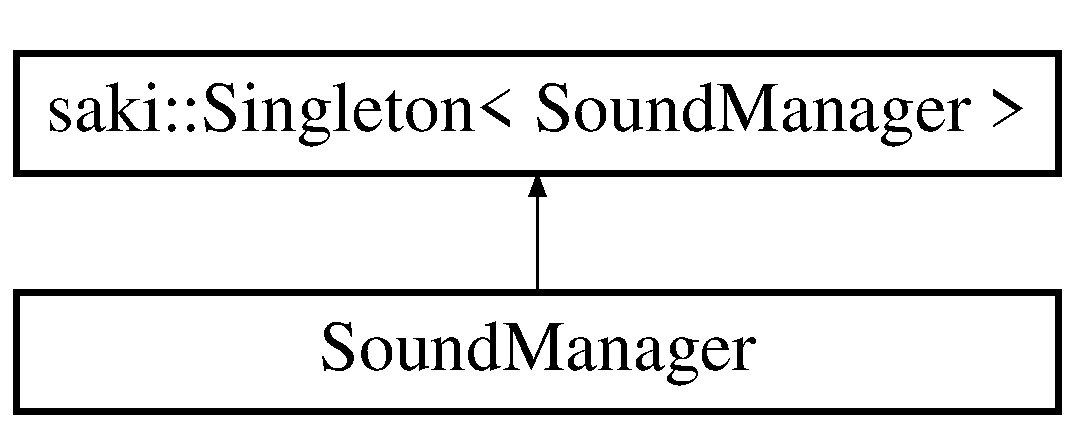
\includegraphics[height=2.000000cm]{class_sound_manager}
\end{center}
\end{figure}
\subsection*{公開メンバ関数}
\begin{DoxyCompactItemize}
\item 
std\+::unique\+\_\+ptr$<$ Direct\+X\+::\+Sound\+Effect $>$ \& \mbox{\hyperlink{class_sound_manager_a3ba4b2fe49cdc051f33aa800851f8b98}{Get\+Sound}} (W\+C\+H\+AR $\ast$)
\begin{DoxyCompactList}\small\item\em サウンドを返す \end{DoxyCompactList}\item 
void \mbox{\hyperlink{class_sound_manager_adab2bc016911756ffd973c7d781b5cfb}{Init}} (H\+W\+ND)
\begin{DoxyCompactList}\small\item\em サウンドマネージャークラスの初期化 \end{DoxyCompactList}\item 
void \mbox{\hyperlink{class_sound_manager_aaf241621221cdbefeba78e8b6bc29240}{Update}} ()
\begin{DoxyCompactList}\small\item\em サウンドマネージャーの更新 \end{DoxyCompactList}\item 
void \mbox{\hyperlink{class_sound_manager_abf0d473d0a31323c8e74684976b08e7f}{Destroy}} ()
\begin{DoxyCompactList}\small\item\em サウンドマネージャーの破棄 \end{DoxyCompactList}\item 
auto \mbox{\hyperlink{class_sound_manager_a5a575ac572eb0b50b3bb48b879a1a7e6}{Get\+Engine}} () const
\item 
void \mbox{\hyperlink{class_sound_manager_acc9fb61509f30c7eb9136386eeeb9f94}{Retry\+Audio}} ()
\item 
void \mbox{\hyperlink{class_sound_manager_a97d76cb22596fbb3c85766df0dcde757}{Suspend}} ()
\item 
void \mbox{\hyperlink{class_sound_manager_a6107940d2299131fbd7991a4f222491b}{Resume}} ()
\end{DoxyCompactItemize}
\subsection*{その他の継承メンバ}


\subsection{詳解}
サウンドを管理するクラス 

\subsection{関数詳解}
\mbox{\Hypertarget{class_sound_manager_abf0d473d0a31323c8e74684976b08e7f}\label{class_sound_manager_abf0d473d0a31323c8e74684976b08e7f}} 
\index{Sound\+Manager@{Sound\+Manager}!Destroy@{Destroy}}
\index{Destroy@{Destroy}!Sound\+Manager@{Sound\+Manager}}
\subsubsection{\texorpdfstring{Destroy()}{Destroy()}}
{\footnotesize\ttfamily void Sound\+Manager\+::\+Destroy (\begin{DoxyParamCaption}{ }\end{DoxyParamCaption})}



サウンドマネージャーの破棄 

\mbox{\Hypertarget{class_sound_manager_a5a575ac572eb0b50b3bb48b879a1a7e6}\label{class_sound_manager_a5a575ac572eb0b50b3bb48b879a1a7e6}} 
\index{Sound\+Manager@{Sound\+Manager}!Get\+Engine@{Get\+Engine}}
\index{Get\+Engine@{Get\+Engine}!Sound\+Manager@{Sound\+Manager}}
\subsubsection{\texorpdfstring{Get\+Engine()}{GetEngine()}}
{\footnotesize\ttfamily auto Sound\+Manager\+::\+Get\+Engine (\begin{DoxyParamCaption}{ }\end{DoxyParamCaption}) const\hspace{0.3cm}{\ttfamily [inline]}}

\mbox{\Hypertarget{class_sound_manager_a3ba4b2fe49cdc051f33aa800851f8b98}\label{class_sound_manager_a3ba4b2fe49cdc051f33aa800851f8b98}} 
\index{Sound\+Manager@{Sound\+Manager}!Get\+Sound@{Get\+Sound}}
\index{Get\+Sound@{Get\+Sound}!Sound\+Manager@{Sound\+Manager}}
\subsubsection{\texorpdfstring{Get\+Sound()}{GetSound()}}
{\footnotesize\ttfamily std\+::unique\+\_\+ptr$<$ Direct\+X\+::\+Sound\+Effect $>$ \& Sound\+Manager\+::\+Get\+Sound (\begin{DoxyParamCaption}\item[{W\+C\+H\+AR $\ast$}]{path }\end{DoxyParamCaption})}



サウンドを返す 


\begin{DoxyParams}{引数}
{\em path} & wavファイルのパス\\
\hline
\end{DoxyParams}
同じファイルを2度読み込まないようにする \mbox{\Hypertarget{class_sound_manager_adab2bc016911756ffd973c7d781b5cfb}\label{class_sound_manager_adab2bc016911756ffd973c7d781b5cfb}} 
\index{Sound\+Manager@{Sound\+Manager}!Init@{Init}}
\index{Init@{Init}!Sound\+Manager@{Sound\+Manager}}
\subsubsection{\texorpdfstring{Init()}{Init()}}
{\footnotesize\ttfamily void Sound\+Manager\+::\+Init (\begin{DoxyParamCaption}\item[{H\+W\+ND}]{h\+Wnd }\end{DoxyParamCaption})}



サウンドマネージャークラスの初期化 


\begin{DoxyParams}{引数}
{\em h\+Wnd} & ウィンドウハンドラ \\
\hline
\end{DoxyParams}
\mbox{\Hypertarget{class_sound_manager_a6107940d2299131fbd7991a4f222491b}\label{class_sound_manager_a6107940d2299131fbd7991a4f222491b}} 
\index{Sound\+Manager@{Sound\+Manager}!Resume@{Resume}}
\index{Resume@{Resume}!Sound\+Manager@{Sound\+Manager}}
\subsubsection{\texorpdfstring{Resume()}{Resume()}}
{\footnotesize\ttfamily void Sound\+Manager\+::\+Resume (\begin{DoxyParamCaption}{ }\end{DoxyParamCaption})\hspace{0.3cm}{\ttfamily [inline]}}

\mbox{\Hypertarget{class_sound_manager_acc9fb61509f30c7eb9136386eeeb9f94}\label{class_sound_manager_acc9fb61509f30c7eb9136386eeeb9f94}} 
\index{Sound\+Manager@{Sound\+Manager}!Retry\+Audio@{Retry\+Audio}}
\index{Retry\+Audio@{Retry\+Audio}!Sound\+Manager@{Sound\+Manager}}
\subsubsection{\texorpdfstring{Retry\+Audio()}{RetryAudio()}}
{\footnotesize\ttfamily void Sound\+Manager\+::\+Retry\+Audio (\begin{DoxyParamCaption}{ }\end{DoxyParamCaption})\hspace{0.3cm}{\ttfamily [inline]}}

\mbox{\Hypertarget{class_sound_manager_a97d76cb22596fbb3c85766df0dcde757}\label{class_sound_manager_a97d76cb22596fbb3c85766df0dcde757}} 
\index{Sound\+Manager@{Sound\+Manager}!Suspend@{Suspend}}
\index{Suspend@{Suspend}!Sound\+Manager@{Sound\+Manager}}
\subsubsection{\texorpdfstring{Suspend()}{Suspend()}}
{\footnotesize\ttfamily void Sound\+Manager\+::\+Suspend (\begin{DoxyParamCaption}{ }\end{DoxyParamCaption})\hspace{0.3cm}{\ttfamily [inline]}}

\mbox{\Hypertarget{class_sound_manager_aaf241621221cdbefeba78e8b6bc29240}\label{class_sound_manager_aaf241621221cdbefeba78e8b6bc29240}} 
\index{Sound\+Manager@{Sound\+Manager}!Update@{Update}}
\index{Update@{Update}!Sound\+Manager@{Sound\+Manager}}
\subsubsection{\texorpdfstring{Update()}{Update()}}
{\footnotesize\ttfamily void Sound\+Manager\+::\+Update (\begin{DoxyParamCaption}{ }\end{DoxyParamCaption})}



サウンドマネージャーの更新 



このクラス詳解は次のファイルから抽出されました\+:\begin{DoxyCompactItemize}
\item 
C\+:/\+Users/tokir/\+Documents/\+Git\+Hub/\+Weapon\+Merchant\+Adventure/src/sound/manager/\mbox{\hyperlink{sound__manager_8h}{sound\+\_\+manager.\+h}}\item 
C\+:/\+Users/tokir/\+Documents/\+Git\+Hub/\+Weapon\+Merchant\+Adventure/src/sound/manager/\mbox{\hyperlink{sound__manager_8cpp}{sound\+\_\+manager.\+cpp}}\end{DoxyCompactItemize}

\hypertarget{class_sprite}{}\section{Sprite クラス}
\label{class_sprite}\index{Sprite@{Sprite}}


{\ttfamily \#include $<$sprite.\+h$>$}

\subsection*{公開メンバ関数}
\begin{DoxyCompactItemize}
\item 
H\+R\+E\+S\+U\+LT \mbox{\hyperlink{class_sprite_a65b9b470731149992bfa7401ffb676ae}{Init}} (const std\+::string \&, const W\+C\+H\+AR $\ast$, \mbox{\hyperlink{common_8h_ae148fff5818e9444b4ab2288829559bf}{Vec2}} \&, const std\+::string \&=\char`\"{}shader\char`\"{}, const W\+C\+H\+AR $\ast$=L\char`\"{}sprite\+\_\+shader.\+hlsl\char`\"{}, const W\+C\+H\+AR $\ast$=L\char`\"{}sprite\+\_\+shader.\+hlsl\char`\"{}, const float=1, const float=1, const float=1, const float=1)
\item 
void \mbox{\hyperlink{class_sprite_a23296a54e3165adbbeb2b5351d04b921}{Render}} (const \mbox{\hyperlink{common_8h_a1c43cb8f0d8a41901f3ce4c67dbbce20}{Transform}} \&, const bool=true)
\item 
void \mbox{\hyperlink{class_sprite_a0a3daa8677d1205981e27bd698025afa}{Color\+Change}} (const float r, const float g, const float b, const float a)
\end{DoxyCompactItemize}
\subsection*{公開変数類}
\begin{DoxyCompactItemize}
\item 
\mbox{\hyperlink{common_8h_ae148fff5818e9444b4ab2288829559bf}{Vec2}} \mbox{\hyperlink{class_sprite_aac62c18a9b678d357f3465d45b2e6ebd}{slice\+\_\+num}}
\item 
\mbox{\hyperlink{common_8h_ae148fff5818e9444b4ab2288829559bf}{Vec2}} \mbox{\hyperlink{class_sprite_a5c96c0e7d46a79740a5fe9e71e9f132b}{prev\+\_\+slice}}
\item 
\mbox{\hyperlink{common_8h_ae148fff5818e9444b4ab2288829559bf}{Vec2}} \mbox{\hyperlink{class_sprite_a7d4903c9693bbb41094b395fe587bf47}{current\+\_\+slice}}
\item 
\mbox{\hyperlink{common_8h_ae148fff5818e9444b4ab2288829559bf}{Vec2}} \mbox{\hyperlink{class_sprite_afb8f3dc3f60aaa09306153d50e4243c9}{texture\+\_\+size}}
\item 
bool \mbox{\hyperlink{class_sprite_ae561a927089192371cff0c1b7402593b}{is\+\_\+ui\+\_\+image}} = false
\item 
float \mbox{\hyperlink{class_sprite_a4e306b23bbc378d1d973ca61084ebd9e}{percent}} = 1.\+0f
\end{DoxyCompactItemize}
\subsection*{静的公開変数類}
\begin{DoxyCompactItemize}
\item 
static int \mbox{\hyperlink{class_sprite_a9acc35b192b4150fe31b9386f7f9fc78}{depth}} = 9999
\item 
static bool \mbox{\hyperlink{class_sprite_ad4340ffd8b88519c28822eb2e9b71bf0}{has\+\_\+target}} = false
\item 
static float \mbox{\hyperlink{class_sprite_add18808500d3dca23d496757bf10259a}{target\+\_\+x}} = 0
\end{DoxyCompactItemize}


\subsection{関数詳解}
\mbox{\Hypertarget{class_sprite_a0a3daa8677d1205981e27bd698025afa}\label{class_sprite_a0a3daa8677d1205981e27bd698025afa}} 
\index{Sprite@{Sprite}!Color\+Change@{Color\+Change}}
\index{Color\+Change@{Color\+Change}!Sprite@{Sprite}}
\subsubsection{\texorpdfstring{Color\+Change()}{ColorChange()}}
{\footnotesize\ttfamily void Sprite\+::\+Color\+Change (\begin{DoxyParamCaption}\item[{const float}]{r,  }\item[{const float}]{g,  }\item[{const float}]{b,  }\item[{const float}]{a }\end{DoxyParamCaption})\hspace{0.3cm}{\ttfamily [inline]}}

\mbox{\Hypertarget{class_sprite_a65b9b470731149992bfa7401ffb676ae}\label{class_sprite_a65b9b470731149992bfa7401ffb676ae}} 
\index{Sprite@{Sprite}!Init@{Init}}
\index{Init@{Init}!Sprite@{Sprite}}
\subsubsection{\texorpdfstring{Init()}{Init()}}
{\footnotesize\ttfamily H\+R\+E\+S\+U\+LT Sprite\+::\+Init (\begin{DoxyParamCaption}\item[{const std\+::string \&}]{texture\+\_\+name,  }\item[{const W\+C\+H\+AR $\ast$}]{texture\+\_\+path,  }\item[{\mbox{\hyperlink{common_8h_ae148fff5818e9444b4ab2288829559bf}{Vec2}} \&}]{size,  }\item[{const std\+::string \&}]{shader\+\_\+name = {\ttfamily \char`\"{}shader\char`\"{}},  }\item[{const W\+C\+H\+AR $\ast$}]{v\+\_\+shader\+\_\+path = {\ttfamily L\char`\"{}sprite\+\_\+shader.hlsl\char`\"{}},  }\item[{const W\+C\+H\+AR $\ast$}]{p\+\_\+shader\+\_\+path = {\ttfamily L\char`\"{}sprite\+\_\+shader.hlsl\char`\"{}},  }\item[{const float}]{slice\+\_\+h\+\_\+num = {\ttfamily 1},  }\item[{const float}]{slice\+\_\+v\+\_\+num = {\ttfamily 1},  }\item[{const float}]{slice\+\_\+h\+\_\+init = {\ttfamily 1},  }\item[{const float}]{slice\+\_\+v\+\_\+init = {\ttfamily 1} }\end{DoxyParamCaption})}

\mbox{\Hypertarget{class_sprite_a23296a54e3165adbbeb2b5351d04b921}\label{class_sprite_a23296a54e3165adbbeb2b5351d04b921}} 
\index{Sprite@{Sprite}!Render@{Render}}
\index{Render@{Render}!Sprite@{Sprite}}
\subsubsection{\texorpdfstring{Render()}{Render()}}
{\footnotesize\ttfamily void Sprite\+::\+Render (\begin{DoxyParamCaption}\item[{const \mbox{\hyperlink{common_8h_a1c43cb8f0d8a41901f3ce4c67dbbce20}{Transform}} \&}]{transform,  }\item[{const bool}]{camera\+\_\+affected = {\ttfamily true} }\end{DoxyParamCaption})}



\subsection{メンバ詳解}
\mbox{\Hypertarget{class_sprite_a7d4903c9693bbb41094b395fe587bf47}\label{class_sprite_a7d4903c9693bbb41094b395fe587bf47}} 
\index{Sprite@{Sprite}!current\+\_\+slice@{current\+\_\+slice}}
\index{current\+\_\+slice@{current\+\_\+slice}!Sprite@{Sprite}}
\subsubsection{\texorpdfstring{current\+\_\+slice}{current\_slice}}
{\footnotesize\ttfamily \mbox{\hyperlink{common_8h_ae148fff5818e9444b4ab2288829559bf}{Vec2}} Sprite\+::current\+\_\+slice}

\mbox{\Hypertarget{class_sprite_a9acc35b192b4150fe31b9386f7f9fc78}\label{class_sprite_a9acc35b192b4150fe31b9386f7f9fc78}} 
\index{Sprite@{Sprite}!depth@{depth}}
\index{depth@{depth}!Sprite@{Sprite}}
\subsubsection{\texorpdfstring{depth}{depth}}
{\footnotesize\ttfamily int Sprite\+::depth = 9999\hspace{0.3cm}{\ttfamily [static]}}

\mbox{\Hypertarget{class_sprite_ad4340ffd8b88519c28822eb2e9b71bf0}\label{class_sprite_ad4340ffd8b88519c28822eb2e9b71bf0}} 
\index{Sprite@{Sprite}!has\+\_\+target@{has\+\_\+target}}
\index{has\+\_\+target@{has\+\_\+target}!Sprite@{Sprite}}
\subsubsection{\texorpdfstring{has\+\_\+target}{has\_target}}
{\footnotesize\ttfamily bool Sprite\+::has\+\_\+target = false\hspace{0.3cm}{\ttfamily [static]}}

\mbox{\Hypertarget{class_sprite_ae561a927089192371cff0c1b7402593b}\label{class_sprite_ae561a927089192371cff0c1b7402593b}} 
\index{Sprite@{Sprite}!is\+\_\+ui\+\_\+image@{is\+\_\+ui\+\_\+image}}
\index{is\+\_\+ui\+\_\+image@{is\+\_\+ui\+\_\+image}!Sprite@{Sprite}}
\subsubsection{\texorpdfstring{is\+\_\+ui\+\_\+image}{is\_ui\_image}}
{\footnotesize\ttfamily bool Sprite\+::is\+\_\+ui\+\_\+image = false}

\mbox{\Hypertarget{class_sprite_a4e306b23bbc378d1d973ca61084ebd9e}\label{class_sprite_a4e306b23bbc378d1d973ca61084ebd9e}} 
\index{Sprite@{Sprite}!percent@{percent}}
\index{percent@{percent}!Sprite@{Sprite}}
\subsubsection{\texorpdfstring{percent}{percent}}
{\footnotesize\ttfamily float Sprite\+::percent = 1.\+0f}

\mbox{\Hypertarget{class_sprite_a5c96c0e7d46a79740a5fe9e71e9f132b}\label{class_sprite_a5c96c0e7d46a79740a5fe9e71e9f132b}} 
\index{Sprite@{Sprite}!prev\+\_\+slice@{prev\+\_\+slice}}
\index{prev\+\_\+slice@{prev\+\_\+slice}!Sprite@{Sprite}}
\subsubsection{\texorpdfstring{prev\+\_\+slice}{prev\_slice}}
{\footnotesize\ttfamily \mbox{\hyperlink{common_8h_ae148fff5818e9444b4ab2288829559bf}{Vec2}} Sprite\+::prev\+\_\+slice}

\mbox{\Hypertarget{class_sprite_aac62c18a9b678d357f3465d45b2e6ebd}\label{class_sprite_aac62c18a9b678d357f3465d45b2e6ebd}} 
\index{Sprite@{Sprite}!slice\+\_\+num@{slice\+\_\+num}}
\index{slice\+\_\+num@{slice\+\_\+num}!Sprite@{Sprite}}
\subsubsection{\texorpdfstring{slice\+\_\+num}{slice\_num}}
{\footnotesize\ttfamily \mbox{\hyperlink{common_8h_ae148fff5818e9444b4ab2288829559bf}{Vec2}} Sprite\+::slice\+\_\+num}

\mbox{\Hypertarget{class_sprite_add18808500d3dca23d496757bf10259a}\label{class_sprite_add18808500d3dca23d496757bf10259a}} 
\index{Sprite@{Sprite}!target\+\_\+x@{target\+\_\+x}}
\index{target\+\_\+x@{target\+\_\+x}!Sprite@{Sprite}}
\subsubsection{\texorpdfstring{target\+\_\+x}{target\_x}}
{\footnotesize\ttfamily float Sprite\+::target\+\_\+x = 0\hspace{0.3cm}{\ttfamily [static]}}

\mbox{\Hypertarget{class_sprite_afb8f3dc3f60aaa09306153d50e4243c9}\label{class_sprite_afb8f3dc3f60aaa09306153d50e4243c9}} 
\index{Sprite@{Sprite}!texture\+\_\+size@{texture\+\_\+size}}
\index{texture\+\_\+size@{texture\+\_\+size}!Sprite@{Sprite}}
\subsubsection{\texorpdfstring{texture\+\_\+size}{texture\_size}}
{\footnotesize\ttfamily \mbox{\hyperlink{common_8h_ae148fff5818e9444b4ab2288829559bf}{Vec2}} Sprite\+::texture\+\_\+size}



このクラス詳解は次のファイルから抽出されました\+:\begin{DoxyCompactItemize}
\item 
C\+:/\+Users/tokir/\+Documents/\+Git\+Hub/\+Weapon\+Merchant\+Adventure/src/src/sprite/\mbox{\hyperlink{sprite_8h}{sprite.\+h}}\item 
C\+:/\+Users/tokir/\+Documents/\+Git\+Hub/\+Weapon\+Merchant\+Adventure/src/src/sprite/\mbox{\hyperlink{sprite_8cpp}{sprite.\+cpp}}\end{DoxyCompactItemize}

\hypertarget{class_square_collider}{}\section{Square\+Collider クラス}
\label{class_square_collider}\index{Square\+Collider@{Square\+Collider}}


四角形コライダクラス  




{\ttfamily \#include $<$square\+\_\+collider.\+h$>$}

Square\+Collider の継承関係図\begin{figure}[H]
\begin{center}
\leavevmode
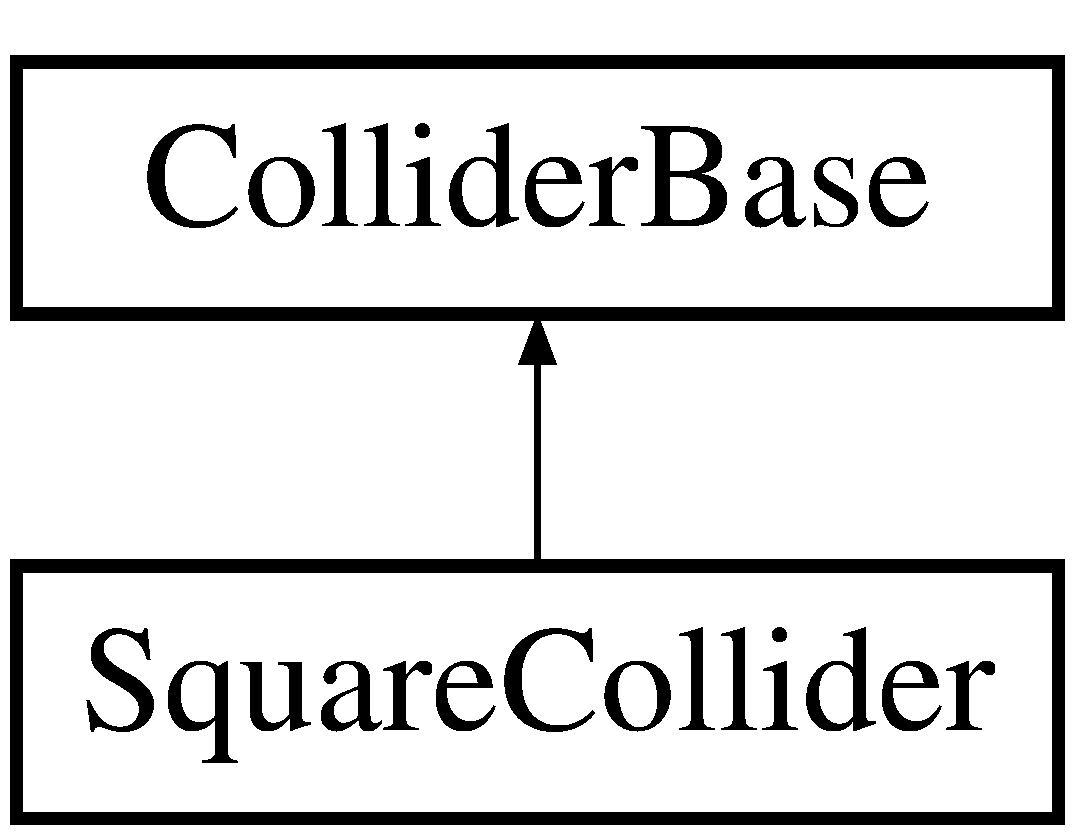
\includegraphics[height=2.000000cm]{class_square_collider}
\end{center}
\end{figure}
\subsection*{公開メンバ関数}
\begin{DoxyCompactItemize}
\item 
\mbox{\hyperlink{class_square_collider_a354753b61e7fa39cb5e7aadcddb78910}{Square\+Collider}} (\mbox{\hyperlink{class_object_base}{Object\+Base}} $\ast$, bool=false, bool=false)
\begin{DoxyCompactList}\small\item\em コンストラクタ \end{DoxyCompactList}\item 
void \mbox{\hyperlink{class_square_collider_a382870e5f0bc29b4f38eb476ecb2fd68}{Set\+Status}} (const \mbox{\hyperlink{common_8h_ab1cb35b3a17c398d8ef71d5f779808bf}{Vec3}} \&pos, const float w, const float h, const \mbox{\hyperlink{common_8h_ab1cb35b3a17c398d8ef71d5f779808bf}{Vec3}} \&scale)
\begin{DoxyCompactList}\small\item\em 当たり判定のステータスをセットする \end{DoxyCompactList}\item 
void \mbox{\hyperlink{class_square_collider_ac250db865d0755fc8731f1660397943d}{Collision\+Extrusion}} (const \mbox{\hyperlink{common_8h_ae148fff5818e9444b4ab2288829559bf}{Vec2}} \&)
\begin{DoxyCompactList}\small\item\em 当たったときの押し出し \end{DoxyCompactList}\item 
const Square\+Status \& \mbox{\hyperlink{class_square_collider_ac437bc1bed951c82ca25d2b17a7b2e0f}{Get\+Status}} () const
\begin{DoxyCompactList}\small\item\em 当たり判定のステータスを返す \end{DoxyCompactList}\item 
void \mbox{\hyperlink{class_square_collider_a83273e0e63692aa8020b8deedd456886}{Destroy}} ()
\begin{DoxyCompactList}\small\item\em 四角形のコライダの破棄 \end{DoxyCompactList}\item 
\mbox{\hyperlink{class_square_collider}{Square\+Collider}} \& \mbox{\hyperlink{class_square_collider_aaa648559b58219a455333f3a100c1d67}{operator=}} (const \mbox{\hyperlink{class_square_collider}{Square\+Collider}} \&other)
\begin{DoxyCompactList}\small\item\em コピー代入演算子 \end{DoxyCompactList}\end{DoxyCompactItemize}
\subsection*{その他の継承メンバ}


\subsection{詳解}
四角形コライダクラス 

\subsection{構築子と解体子}
\mbox{\Hypertarget{class_square_collider_a354753b61e7fa39cb5e7aadcddb78910}\label{class_square_collider_a354753b61e7fa39cb5e7aadcddb78910}} 
\index{Square\+Collider@{Square\+Collider}!Square\+Collider@{Square\+Collider}}
\index{Square\+Collider@{Square\+Collider}!Square\+Collider@{Square\+Collider}}
\subsubsection{\texorpdfstring{Square\+Collider()}{SquareCollider()}}
{\footnotesize\ttfamily Square\+Collider\+::\+Square\+Collider (\begin{DoxyParamCaption}\item[{\mbox{\hyperlink{class_object_base}{Object\+Base}} $\ast$}]{obj,  }\item[{bool}]{\+\_\+is\+\_\+trigger = {\ttfamily false},  }\item[{bool}]{\+\_\+is\+\_\+static = {\ttfamily false} }\end{DoxyParamCaption})}



コンストラクタ 


\begin{DoxyParams}{引数}
{\em obj} & オブジェクト \\
\hline
{\em \+\_\+is\+\_\+trigger} & 当たったときに透けるかどうか \\
\hline
{\em \+\_\+is\+\_\+static} & 静的かどうか \\
\hline
\end{DoxyParams}


\subsection{関数詳解}
\mbox{\Hypertarget{class_square_collider_ac250db865d0755fc8731f1660397943d}\label{class_square_collider_ac250db865d0755fc8731f1660397943d}} 
\index{Square\+Collider@{Square\+Collider}!Collision\+Extrusion@{Collision\+Extrusion}}
\index{Collision\+Extrusion@{Collision\+Extrusion}!Square\+Collider@{Square\+Collider}}
\subsubsection{\texorpdfstring{Collision\+Extrusion()}{CollisionExtrusion()}}
{\footnotesize\ttfamily void Square\+Collider\+::\+Collision\+Extrusion (\begin{DoxyParamCaption}\item[{const \mbox{\hyperlink{common_8h_ae148fff5818e9444b4ab2288829559bf}{Vec2}} \&}]{pos }\end{DoxyParamCaption})}



当たったときの押し出し 


\begin{DoxyParams}{引数}
{\em pos} & 移動先\\
\hline
\end{DoxyParams}
加算減算にしない理由はfloatの誤差が起きてバグらないようにするため \mbox{\Hypertarget{class_square_collider_a83273e0e63692aa8020b8deedd456886}\label{class_square_collider_a83273e0e63692aa8020b8deedd456886}} 
\index{Square\+Collider@{Square\+Collider}!Destroy@{Destroy}}
\index{Destroy@{Destroy}!Square\+Collider@{Square\+Collider}}
\subsubsection{\texorpdfstring{Destroy()}{Destroy()}}
{\footnotesize\ttfamily void Square\+Collider\+::\+Destroy (\begin{DoxyParamCaption}{ }\end{DoxyParamCaption})}



四角形のコライダの破棄 

\mbox{\Hypertarget{class_square_collider_ac437bc1bed951c82ca25d2b17a7b2e0f}\label{class_square_collider_ac437bc1bed951c82ca25d2b17a7b2e0f}} 
\index{Square\+Collider@{Square\+Collider}!Get\+Status@{Get\+Status}}
\index{Get\+Status@{Get\+Status}!Square\+Collider@{Square\+Collider}}
\subsubsection{\texorpdfstring{Get\+Status()}{GetStatus()}}
{\footnotesize\ttfamily const Square\+Status\& Square\+Collider\+::\+Get\+Status (\begin{DoxyParamCaption}{ }\end{DoxyParamCaption}) const\hspace{0.3cm}{\ttfamily [inline]}}



当たり判定のステータスを返す 

\begin{DoxyReturn}{戻り値}
const Square\+Status\& ステータス 
\end{DoxyReturn}
\mbox{\Hypertarget{class_square_collider_aaa648559b58219a455333f3a100c1d67}\label{class_square_collider_aaa648559b58219a455333f3a100c1d67}} 
\index{Square\+Collider@{Square\+Collider}!operator=@{operator=}}
\index{operator=@{operator=}!Square\+Collider@{Square\+Collider}}
\subsubsection{\texorpdfstring{operator=()}{operator=()}}
{\footnotesize\ttfamily \mbox{\hyperlink{class_square_collider}{Square\+Collider}} \& Square\+Collider\+::operator= (\begin{DoxyParamCaption}\item[{const \mbox{\hyperlink{class_square_collider}{Square\+Collider}} \&}]{other }\end{DoxyParamCaption})}



コピー代入演算子 

\mbox{\Hypertarget{class_square_collider_a382870e5f0bc29b4f38eb476ecb2fd68}\label{class_square_collider_a382870e5f0bc29b4f38eb476ecb2fd68}} 
\index{Square\+Collider@{Square\+Collider}!Set\+Status@{Set\+Status}}
\index{Set\+Status@{Set\+Status}!Square\+Collider@{Square\+Collider}}
\subsubsection{\texorpdfstring{Set\+Status()}{SetStatus()}}
{\footnotesize\ttfamily void Square\+Collider\+::\+Set\+Status (\begin{DoxyParamCaption}\item[{const \mbox{\hyperlink{common_8h_ab1cb35b3a17c398d8ef71d5f779808bf}{Vec3}} \&}]{pos,  }\item[{const float}]{w,  }\item[{const float}]{h,  }\item[{const \mbox{\hyperlink{common_8h_ab1cb35b3a17c398d8ef71d5f779808bf}{Vec3}} \&}]{scale }\end{DoxyParamCaption})}



当たり判定のステータスをセットする 


\begin{DoxyParams}{引数}
{\em pos} & センターの位置 \\
\hline
{\em w,h} & 幅、高さ \\
\hline
{\em scale} & 拡大・縮小 \\
\hline
\end{DoxyParams}


このクラス詳解は次のファイルから抽出されました\+:\begin{DoxyCompactItemize}
\item 
C\+:/\+Users/tokir/\+Documents/\+Git\+Hub/\+Weapon\+Merchant\+Adventure/src/src/collider/square/\mbox{\hyperlink{square__collider_8h}{square\+\_\+collider.\+h}}\item 
C\+:/\+Users/tokir/\+Documents/\+Git\+Hub/\+Weapon\+Merchant\+Adventure/src/src/collider/square/\mbox{\hyperlink{square__collider_8cpp}{square\+\_\+collider.\+cpp}}\end{DoxyCompactItemize}

\hypertarget{class_static_object}{}\section{Static\+Object クラス}
\label{class_static_object}\index{Static\+Object@{Static\+Object}}


動かないオブジェクトのスーパークラス  




{\ttfamily \#include $<$static\+\_\+object.\+h$>$}

Static\+Object の継承関係図\begin{figure}[H]
\begin{center}
\leavevmode
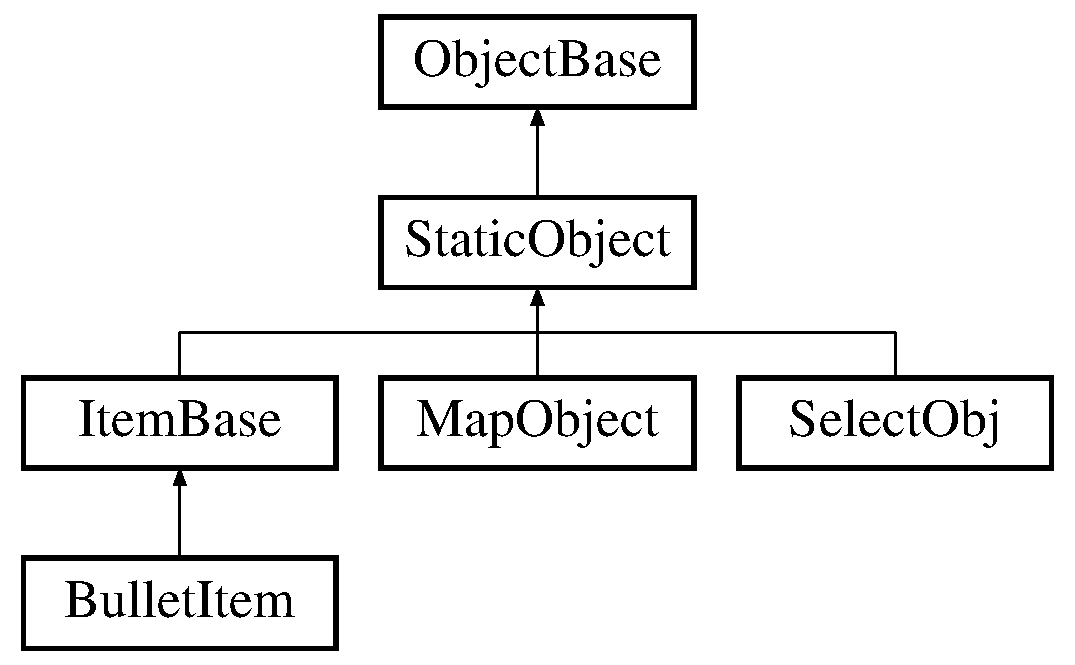
\includegraphics[height=4.000000cm]{class_static_object}
\end{center}
\end{figure}
\subsection*{公開メンバ関数}
\begin{DoxyCompactItemize}
\item 
\mbox{\hyperlink{class_static_object_a2a8e918ddfe5c6723b88b9f5c4156472}{Static\+Object}} ()
\begin{DoxyCompactList}\small\item\em コンストラクタ \end{DoxyCompactList}\item 
\mbox{\hyperlink{class_static_object_a0e1518e656ce5ba408cb69f14ee3066b}{Static\+Object}} (const \mbox{\hyperlink{class_static_object}{Static\+Object}} \&other)
\item 
\mbox{\hyperlink{class_static_object}{Static\+Object}} \& \mbox{\hyperlink{class_static_object_aa2a0526bd19e479ea4d1e5da236c1bf3}{operator=}} (const \mbox{\hyperlink{class_static_object}{Static\+Object}} \&other)
\begin{DoxyCompactList}\small\item\em コピー代入演算子 \end{DoxyCompactList}\item 
virtual void \mbox{\hyperlink{class_static_object_a8e9fb321b4f8f12c4bec1bc66853512f}{Destroy}} ()
\item 
virtual void \mbox{\hyperlink{class_static_object_a64c8803ff881d578d103413e299dbf7f}{Collision}} (\mbox{\hyperlink{class_object_base}{Object\+Base}} $\ast$, \mbox{\hyperlink{common_8h_ae148fff5818e9444b4ab2288829559bf}{Vec2}})
\item 
virtual \mbox{\hyperlink{class_static_object_ac27301fc3d8d22aff5664f592c375cd8}{$\sim$\+Static\+Object}} ()
\item 
void \mbox{\hyperlink{class_static_object_a44408a8130d19f7284fe4daaab87c712}{Set\+Color}} (const float, const float, const float, const float)
\end{DoxyCompactItemize}
\subsection*{限定公開メンバ関数}
\begin{DoxyCompactItemize}
\item 
void \mbox{\hyperlink{class_static_object_afec57009537695c4715386120a619942}{Render\+Process}} (bool)
\begin{DoxyCompactList}\small\item\em 描画 \end{DoxyCompactList}\item 
virtual void \mbox{\hyperlink{class_static_object_afa0709f50495338a23c1140062a567af}{Init\+Process}} ()
\item 
virtual void \mbox{\hyperlink{class_static_object_a7fa678c3c4032bb6e9417f93a8bb895c}{Update\+Process}} ()
\item 
virtual void \mbox{\hyperlink{class_static_object_a36379eb74b66c1586f1cc678a85c52c1}{Collision\+Process}} (\mbox{\hyperlink{class_object_base}{Object\+Base}} $\ast$, \mbox{\hyperlink{common_8h_ae148fff5818e9444b4ab2288829559bf}{Vec2}})
\end{DoxyCompactItemize}
\subsection*{その他の継承メンバ}


\subsection{詳解}
動かないオブジェクトのスーパークラス 

\subsection{構築子と解体子}
\mbox{\Hypertarget{class_static_object_a2a8e918ddfe5c6723b88b9f5c4156472}\label{class_static_object_a2a8e918ddfe5c6723b88b9f5c4156472}} 
\index{Static\+Object@{Static\+Object}!Static\+Object@{Static\+Object}}
\index{Static\+Object@{Static\+Object}!Static\+Object@{Static\+Object}}
\subsubsection{\texorpdfstring{Static\+Object()}{StaticObject()}\hspace{0.1cm}{\footnotesize\ttfamily [1/2]}}
{\footnotesize\ttfamily Static\+Object\+::\+Static\+Object (\begin{DoxyParamCaption}{ }\end{DoxyParamCaption})\hspace{0.3cm}{\ttfamily [inline]}}



コンストラクタ 

\mbox{\Hypertarget{class_static_object_a0e1518e656ce5ba408cb69f14ee3066b}\label{class_static_object_a0e1518e656ce5ba408cb69f14ee3066b}} 
\index{Static\+Object@{Static\+Object}!Static\+Object@{Static\+Object}}
\index{Static\+Object@{Static\+Object}!Static\+Object@{Static\+Object}}
\subsubsection{\texorpdfstring{Static\+Object()}{StaticObject()}\hspace{0.1cm}{\footnotesize\ttfamily [2/2]}}
{\footnotesize\ttfamily Static\+Object\+::\+Static\+Object (\begin{DoxyParamCaption}\item[{const \mbox{\hyperlink{class_static_object}{Static\+Object}} \&}]{other }\end{DoxyParamCaption})\hspace{0.3cm}{\ttfamily [inline]}}

\mbox{\Hypertarget{class_static_object_ac27301fc3d8d22aff5664f592c375cd8}\label{class_static_object_ac27301fc3d8d22aff5664f592c375cd8}} 
\index{Static\+Object@{Static\+Object}!````~Static\+Object@{$\sim$\+Static\+Object}}
\index{````~Static\+Object@{$\sim$\+Static\+Object}!Static\+Object@{Static\+Object}}
\subsubsection{\texorpdfstring{$\sim$\+Static\+Object()}{~StaticObject()}}
{\footnotesize\ttfamily virtual Static\+Object\+::$\sim$\+Static\+Object (\begin{DoxyParamCaption}{ }\end{DoxyParamCaption})\hspace{0.3cm}{\ttfamily [inline]}, {\ttfamily [virtual]}}



\subsection{関数詳解}
\mbox{\Hypertarget{class_static_object_a64c8803ff881d578d103413e299dbf7f}\label{class_static_object_a64c8803ff881d578d103413e299dbf7f}} 
\index{Static\+Object@{Static\+Object}!Collision@{Collision}}
\index{Collision@{Collision}!Static\+Object@{Static\+Object}}
\subsubsection{\texorpdfstring{Collision()}{Collision()}}
{\footnotesize\ttfamily virtual void Static\+Object\+::\+Collision (\begin{DoxyParamCaption}\item[{\mbox{\hyperlink{class_object_base}{Object\+Base}} $\ast$}]{,  }\item[{\mbox{\hyperlink{common_8h_ae148fff5818e9444b4ab2288829559bf}{Vec2}}}]{ }\end{DoxyParamCaption})\hspace{0.3cm}{\ttfamily [inline]}, {\ttfamily [virtual]}}



\mbox{\hyperlink{class_object_base_a3e1db79dfa119be067d816c22d09839d}{Object\+Base}}を再実装しています。



\mbox{\hyperlink{class_item_base_ae5c2bcf78c74126a6f76783ca927c7ab}{Item\+Base}}, \mbox{\hyperlink{class_map_object_a76b9161f2723272ad361d0b190e46245}{Map\+Object}}, \mbox{\hyperlink{class_select_obj_a497ff683aefe9bf77201eee1e3948e15}{Select\+Obj}}で再実装されています。

\mbox{\Hypertarget{class_static_object_a36379eb74b66c1586f1cc678a85c52c1}\label{class_static_object_a36379eb74b66c1586f1cc678a85c52c1}} 
\index{Static\+Object@{Static\+Object}!Collision\+Process@{Collision\+Process}}
\index{Collision\+Process@{Collision\+Process}!Static\+Object@{Static\+Object}}
\subsubsection{\texorpdfstring{Collision\+Process()}{CollisionProcess()}}
{\footnotesize\ttfamily virtual void Static\+Object\+::\+Collision\+Process (\begin{DoxyParamCaption}\item[{\mbox{\hyperlink{class_object_base}{Object\+Base}} $\ast$}]{,  }\item[{\mbox{\hyperlink{common_8h_ae148fff5818e9444b4ab2288829559bf}{Vec2}}}]{ }\end{DoxyParamCaption})\hspace{0.3cm}{\ttfamily [inline]}, {\ttfamily [protected]}, {\ttfamily [virtual]}}

\mbox{\Hypertarget{class_static_object_a8e9fb321b4f8f12c4bec1bc66853512f}\label{class_static_object_a8e9fb321b4f8f12c4bec1bc66853512f}} 
\index{Static\+Object@{Static\+Object}!Destroy@{Destroy}}
\index{Destroy@{Destroy}!Static\+Object@{Static\+Object}}
\subsubsection{\texorpdfstring{Destroy()}{Destroy()}}
{\footnotesize\ttfamily virtual void Static\+Object\+::\+Destroy (\begin{DoxyParamCaption}{ }\end{DoxyParamCaption})\hspace{0.3cm}{\ttfamily [inline]}, {\ttfamily [virtual]}}



\mbox{\hyperlink{class_object_base_a7fa4c548153c3af20f89673ffea809af}{Object\+Base}}を実装しています。



\mbox{\hyperlink{class_map_object_ad4bcfdc33bd945a9aa5e50a57c2704bc}{Map\+Object}}, \mbox{\hyperlink{class_item_base_ab34d53b8f3442da77466ba1b9132386e}{Item\+Base}}, \mbox{\hyperlink{class_select_obj_ad3a5fdc41a9e5753f99bae7ad289888f}{Select\+Obj}}で再実装されています。

\mbox{\Hypertarget{class_static_object_afa0709f50495338a23c1140062a567af}\label{class_static_object_afa0709f50495338a23c1140062a567af}} 
\index{Static\+Object@{Static\+Object}!Init\+Process@{Init\+Process}}
\index{Init\+Process@{Init\+Process}!Static\+Object@{Static\+Object}}
\subsubsection{\texorpdfstring{Init\+Process()}{InitProcess()}}
{\footnotesize\ttfamily virtual void Static\+Object\+::\+Init\+Process (\begin{DoxyParamCaption}{ }\end{DoxyParamCaption})\hspace{0.3cm}{\ttfamily [inline]}, {\ttfamily [protected]}, {\ttfamily [virtual]}}



\mbox{\hyperlink{class_object_base_af133f36f2bca1dcfd962e2cfac61ab51}{Object\+Base}}を実装しています。



\mbox{\hyperlink{class_map_object_a3043cddb8aaad0eab27a076e9bee0284}{Map\+Object}}, \mbox{\hyperlink{class_select_obj_a09c9e1a54f4605eda5bb6e18887c2654}{Select\+Obj}}, \mbox{\hyperlink{class_item_base_a772804cb3c663b35e44d49913d1f1cef}{Item\+Base}}で再実装されています。

\mbox{\Hypertarget{class_static_object_aa2a0526bd19e479ea4d1e5da236c1bf3}\label{class_static_object_aa2a0526bd19e479ea4d1e5da236c1bf3}} 
\index{Static\+Object@{Static\+Object}!operator=@{operator=}}
\index{operator=@{operator=}!Static\+Object@{Static\+Object}}
\subsubsection{\texorpdfstring{operator=()}{operator=()}}
{\footnotesize\ttfamily \mbox{\hyperlink{class_static_object}{Static\+Object}}\& Static\+Object\+::operator= (\begin{DoxyParamCaption}\item[{const \mbox{\hyperlink{class_static_object}{Static\+Object}} \&}]{other }\end{DoxyParamCaption})\hspace{0.3cm}{\ttfamily [inline]}}



コピー代入演算子 

\mbox{\Hypertarget{class_static_object_afec57009537695c4715386120a619942}\label{class_static_object_afec57009537695c4715386120a619942}} 
\index{Static\+Object@{Static\+Object}!Render\+Process@{Render\+Process}}
\index{Render\+Process@{Render\+Process}!Static\+Object@{Static\+Object}}
\subsubsection{\texorpdfstring{Render\+Process()}{RenderProcess()}}
{\footnotesize\ttfamily void Static\+Object\+::\+Render\+Process (\begin{DoxyParamCaption}\item[{bool}]{camera\+\_\+affected }\end{DoxyParamCaption})\hspace{0.3cm}{\ttfamily [protected]}, {\ttfamily [virtual]}}



描画 


\begin{DoxyParams}{引数}
{\em camera\+\_\+affected} & カメラの位置によって位置を変えるかどうか \\
\hline
\end{DoxyParams}


\mbox{\hyperlink{class_object_base_aeac51d868beeb7f7fe900407b76b93a2}{Object\+Base}}を実装しています。

\mbox{\Hypertarget{class_static_object_a44408a8130d19f7284fe4daaab87c712}\label{class_static_object_a44408a8130d19f7284fe4daaab87c712}} 
\index{Static\+Object@{Static\+Object}!Set\+Color@{Set\+Color}}
\index{Set\+Color@{Set\+Color}!Static\+Object@{Static\+Object}}
\subsubsection{\texorpdfstring{Set\+Color()}{SetColor()}}
{\footnotesize\ttfamily void Static\+Object\+::\+Set\+Color (\begin{DoxyParamCaption}\item[{const float}]{r,  }\item[{const float}]{g,  }\item[{const float}]{b,  }\item[{const float}]{a }\end{DoxyParamCaption})}

\mbox{\Hypertarget{class_static_object_a7fa678c3c4032bb6e9417f93a8bb895c}\label{class_static_object_a7fa678c3c4032bb6e9417f93a8bb895c}} 
\index{Static\+Object@{Static\+Object}!Update\+Process@{Update\+Process}}
\index{Update\+Process@{Update\+Process}!Static\+Object@{Static\+Object}}
\subsubsection{\texorpdfstring{Update\+Process()}{UpdateProcess()}}
{\footnotesize\ttfamily virtual void Static\+Object\+::\+Update\+Process (\begin{DoxyParamCaption}{ }\end{DoxyParamCaption})\hspace{0.3cm}{\ttfamily [inline]}, {\ttfamily [protected]}, {\ttfamily [virtual]}}



\mbox{\hyperlink{class_object_base_a8b5b72b363a419767efde0b0e692ea95}{Object\+Base}}を実装しています。



\mbox{\hyperlink{class_map_object_ab6b8849f15175417eca94b2703945e4b}{Map\+Object}}, \mbox{\hyperlink{class_item_base_a8edff8edcf884f9590f973fd05d218bc}{Item\+Base}}, \mbox{\hyperlink{class_select_obj_a4788d957629f0b69dc78166f09f949bb}{Select\+Obj}}で再実装されています。



このクラス詳解は次のファイルから抽出されました\+:\begin{DoxyCompactItemize}
\item 
C\+:/\+Users/tokir/\+Documents/\+Git\+Hub/\+Weapon\+Merchant\+Adventure/src/src/object/base/static/\mbox{\hyperlink{static__object_8h}{static\+\_\+object.\+h}}\item 
C\+:/\+Users/tokir/\+Documents/\+Git\+Hub/\+Weapon\+Merchant\+Adventure/src/src/object/base/static/\mbox{\hyperlink{static__object_8cpp}{static\+\_\+object.\+cpp}}\end{DoxyCompactItemize}

\hypertarget{class_status}{}\section{Status クラス}
\label{class_status}\index{Status@{Status}}


ステータスクラス  




{\ttfamily \#include $<$status.\+h$>$}

\subsection*{公開メンバ関数}
\begin{DoxyCompactItemize}
\item 
void \mbox{\hyperlink{class_status_a04cf2752224db252d7694c2caf5caf83}{Init}} (const float hp, const float attack, const float defense)
\begin{DoxyCompactList}\small\item\em 初期化 \end{DoxyCompactList}\item 
\mbox{\hyperlink{class_status}{Status}} \& \mbox{\hyperlink{class_status_abc76064ed2504493c3bbc0f287a49525}{operator=}} (const \mbox{\hyperlink{class_status}{Status}} \&other)
\end{DoxyCompactItemize}
\subsection*{公開変数類}
\begin{DoxyCompactItemize}
\item 
float \mbox{\hyperlink{class_status_a0ec54fdb31c6c4b1a23b22742e6babb4}{HP}}
\item 
float \mbox{\hyperlink{class_status_aede601b020ef15845b86d631a46f8980}{Attack}}
\item 
float \mbox{\hyperlink{class_status_aee944c63904ca1b6b3b04e24b2a9ac12}{Defense}}
\end{DoxyCompactItemize}


\subsection{詳解}
ステータスクラス 

\subsection{関数詳解}
\mbox{\Hypertarget{class_status_a04cf2752224db252d7694c2caf5caf83}\label{class_status_a04cf2752224db252d7694c2caf5caf83}} 
\index{Status@{Status}!Init@{Init}}
\index{Init@{Init}!Status@{Status}}
\subsubsection{\texorpdfstring{Init()}{Init()}}
{\footnotesize\ttfamily void Status\+::\+Init (\begin{DoxyParamCaption}\item[{const float}]{hp,  }\item[{const float}]{attack,  }\item[{const float}]{defense }\end{DoxyParamCaption})\hspace{0.3cm}{\ttfamily [inline]}}



初期化 


\begin{DoxyParams}{引数}
{\em hp} & 初期\+HP \\
\hline
{\em attack} & 攻撃力 \\
\hline
{\em defense} & 防御力 \\
\hline
\end{DoxyParams}
\mbox{\Hypertarget{class_status_abc76064ed2504493c3bbc0f287a49525}\label{class_status_abc76064ed2504493c3bbc0f287a49525}} 
\index{Status@{Status}!operator=@{operator=}}
\index{operator=@{operator=}!Status@{Status}}
\subsubsection{\texorpdfstring{operator=()}{operator=()}}
{\footnotesize\ttfamily \mbox{\hyperlink{class_status}{Status}}\& Status\+::operator= (\begin{DoxyParamCaption}\item[{const \mbox{\hyperlink{class_status}{Status}} \&}]{other }\end{DoxyParamCaption})\hspace{0.3cm}{\ttfamily [inline]}}



\subsection{メンバ詳解}
\mbox{\Hypertarget{class_status_aede601b020ef15845b86d631a46f8980}\label{class_status_aede601b020ef15845b86d631a46f8980}} 
\index{Status@{Status}!Attack@{Attack}}
\index{Attack@{Attack}!Status@{Status}}
\subsubsection{\texorpdfstring{Attack}{Attack}}
{\footnotesize\ttfamily float Status\+::\+Attack}

\mbox{\Hypertarget{class_status_aee944c63904ca1b6b3b04e24b2a9ac12}\label{class_status_aee944c63904ca1b6b3b04e24b2a9ac12}} 
\index{Status@{Status}!Defense@{Defense}}
\index{Defense@{Defense}!Status@{Status}}
\subsubsection{\texorpdfstring{Defense}{Defense}}
{\footnotesize\ttfamily float Status\+::\+Defense}

\mbox{\Hypertarget{class_status_a0ec54fdb31c6c4b1a23b22742e6babb4}\label{class_status_a0ec54fdb31c6c4b1a23b22742e6babb4}} 
\index{Status@{Status}!HP@{HP}}
\index{HP@{HP}!Status@{Status}}
\subsubsection{\texorpdfstring{HP}{HP}}
{\footnotesize\ttfamily float Status\+::\+HP}



このクラス詳解は次のファイルから抽出されました\+:\begin{DoxyCompactItemize}
\item 
C\+:/\+Users/tokir/\+Documents/\+Git\+Hub/\+Weapon\+Merchant\+Adventure/src/status/\mbox{\hyperlink{status_8h}{status.\+h}}\end{DoxyCompactItemize}

\hypertarget{structsaki_1_1subtraction}{}\section{saki\+:\+:subtraction 構造体}
\label{structsaki_1_1subtraction}\index{saki\+::subtraction@{saki\+::subtraction}}


引き算のconstexpr対応した関数オブジェクト  




{\ttfamily \#include $<$subtraction.\+h$>$}

\subsection*{公開メンバ関数}
\begin{DoxyCompactItemize}
\item 
{\footnotesize template$<$typename T1 , typename T2 $>$ }\\constexpr auto \mbox{\hyperlink{structsaki_1_1subtraction_a6c26b497569ef8b5fd7aa213ca675a2c}{operator()}} (const T1 \&t1, const T2 \&t2) const
\end{DoxyCompactItemize}


\subsection{詳解}
引き算のconstexpr対応した関数オブジェクト 

\subsection{関数詳解}
\mbox{\Hypertarget{structsaki_1_1subtraction_a6c26b497569ef8b5fd7aa213ca675a2c}\label{structsaki_1_1subtraction_a6c26b497569ef8b5fd7aa213ca675a2c}} 
\index{saki\+::subtraction@{saki\+::subtraction}!operator()@{operator()}}
\index{operator()@{operator()}!saki\+::subtraction@{saki\+::subtraction}}
\subsubsection{\texorpdfstring{operator()()}{operator()()}}
{\footnotesize\ttfamily template$<$typename T1 , typename T2 $>$ \\
constexpr auto saki\+::subtraction\+::operator() (\begin{DoxyParamCaption}\item[{const T1 \&}]{t1,  }\item[{const T2 \&}]{t2 }\end{DoxyParamCaption}) const\hspace{0.3cm}{\ttfamily [inline]}}



この構造体詳解は次のファイルから抽出されました\+:\begin{DoxyCompactItemize}
\item 
C\+:/\+Users/tokir/\+Documents/\+Git\+Hub/\+Weapon\+Merchant\+Adventure/src/lib/saki/binary\+\_\+operator/\mbox{\hyperlink{subtraction_8h}{subtraction.\+h}}\end{DoxyCompactItemize}

\hypertarget{class_sword}{}\section{Sword クラス}
\label{class_sword}\index{Sword@{Sword}}


剣クラス  




{\ttfamily \#include $<$sword.\+h$>$}

Sword の継承関係図\begin{figure}[H]
\begin{center}
\leavevmode
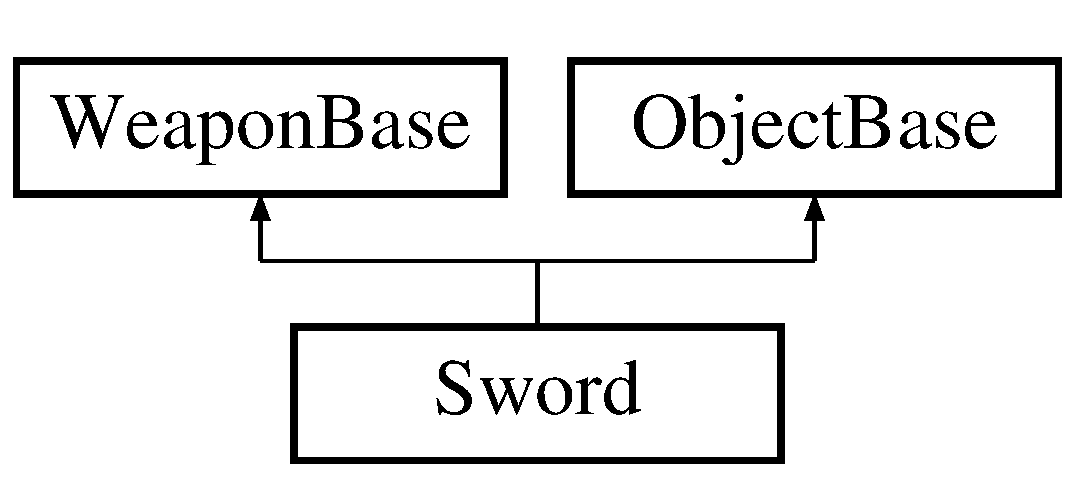
\includegraphics[height=2.000000cm]{class_sword}
\end{center}
\end{figure}
\subsection*{公開メンバ関数}
\begin{DoxyCompactItemize}
\item 
\mbox{\hyperlink{class_sword_af33284e40825ec8ddccd01fa5833be36}{Sword}} ()
\begin{DoxyCompactList}\small\item\em コンストラクタ \end{DoxyCompactList}\item 
\mbox{\hyperlink{class_sword_a6a55d930547584000fcc7c63d47ffabf}{Sword}} (const \mbox{\hyperlink{class_sword}{Sword}} \&s)
\begin{DoxyCompactList}\small\item\em コピーコンストラクタ \end{DoxyCompactList}\item 
\mbox{\hyperlink{class_sword}{Sword}} \& \mbox{\hyperlink{class_sword_a47720cf8f0a44a9a30cf586a188a4730}{operator=}} (const \mbox{\hyperlink{class_sword}{Sword}} \&other)
\begin{DoxyCompactList}\small\item\em 代入演算子 \end{DoxyCompactList}\item 
void \mbox{\hyperlink{class_sword_af9027f627d1db6c0ac21d2aa842cff69}{Weapon\+Start}} () final
\begin{DoxyCompactList}\small\item\em 武器用の初期化 \end{DoxyCompactList}\item 
void \mbox{\hyperlink{class_sword_a5fda2f72829b6256ffc3fb18d9d065e8}{Weapon\+Update}} (const \mbox{\hyperlink{common_8h_ab1cb35b3a17c398d8ef71d5f779808bf}{Vec3}} \&, bool) final
\begin{DoxyCompactList}\small\item\em 武器用の更新 \end{DoxyCompactList}\item 
void \mbox{\hyperlink{class_sword_a3f60d8b24b7847d6a84f0941820b711d}{Weapon\+Destroy}} () final
\begin{DoxyCompactList}\small\item\em 武器用の破棄 \end{DoxyCompactList}\item 
void \mbox{\hyperlink{class_sword_a1dcab625754ca097ad814ee544c6a872}{Collision}} (\mbox{\hyperlink{class_object_base}{Object\+Base}} $\ast$, \mbox{\hyperlink{common_8h_ae148fff5818e9444b4ab2288829559bf}{Vec2}}) final
\begin{DoxyCompactList}\small\item\em 当たったときの反応 \end{DoxyCompactList}\item 
bool \mbox{\hyperlink{class_sword_a6c8642e6a8f1d6152abce6c84bf6d21b}{Attack}} (bool, const \mbox{\hyperlink{common_8h_ab1cb35b3a17c398d8ef71d5f779808bf}{Vec3}} \&) final
\begin{DoxyCompactList}\small\item\em 攻撃 \end{DoxyCompactList}\item 
void \mbox{\hyperlink{class_sword_ac80e3b54ef5572eae1e4760d14383f4f}{Weapon\+Render}} (const \mbox{\hyperlink{common_8h_a1c43cb8f0d8a41901f3ce4c67dbbce20}{Transform}} \&=\mbox{\hyperlink{common_8h_a1c43cb8f0d8a41901f3ce4c67dbbce20}{Transform}}\{ saki\+::vector3\+\_\+zero$<$ float $>$, saki\+::vector3\+\_\+zero$<$ float $>$, saki\+::vector3\+\_\+zero$<$ float $>$ \}) final
\begin{DoxyCompactList}\small\item\em 武器用の描画 \end{DoxyCompactList}\item 
void \mbox{\hyperlink{class_sword_a8473b694775374df4d9b6305cfa82293}{Destroy}} ()
\end{DoxyCompactItemize}
\subsection*{限定公開メンバ関数}
\begin{DoxyCompactItemize}
\item 
void \mbox{\hyperlink{class_sword_a7f5d2c6e6e0104e9a85f600eec14ef6d}{Render\+Process}} (bool) final
\item 
void \mbox{\hyperlink{class_sword_aab0c07888f3aaee1ba25d668ac7c847a}{Init\+Process}} () final
\item 
void \mbox{\hyperlink{class_sword_a3e0221aa5c05ecada9def39fb38c0059}{Update\+Process}} () final
\end{DoxyCompactItemize}
\subsection*{その他の継承メンバ}


\subsection{詳解}
剣クラス 

\subsection{構築子と解体子}
\mbox{\Hypertarget{class_sword_af33284e40825ec8ddccd01fa5833be36}\label{class_sword_af33284e40825ec8ddccd01fa5833be36}} 
\index{Sword@{Sword}!Sword@{Sword}}
\index{Sword@{Sword}!Sword@{Sword}}
\subsubsection{\texorpdfstring{Sword()}{Sword()}\hspace{0.1cm}{\footnotesize\ttfamily [1/2]}}
{\footnotesize\ttfamily Sword\+::\+Sword (\begin{DoxyParamCaption}{ }\end{DoxyParamCaption})}



コンストラクタ 

\mbox{\Hypertarget{class_sword_a6a55d930547584000fcc7c63d47ffabf}\label{class_sword_a6a55d930547584000fcc7c63d47ffabf}} 
\index{Sword@{Sword}!Sword@{Sword}}
\index{Sword@{Sword}!Sword@{Sword}}
\subsubsection{\texorpdfstring{Sword()}{Sword()}\hspace{0.1cm}{\footnotesize\ttfamily [2/2]}}
{\footnotesize\ttfamily Sword\+::\+Sword (\begin{DoxyParamCaption}\item[{const \mbox{\hyperlink{class_sword}{Sword}} \&}]{s }\end{DoxyParamCaption})\hspace{0.3cm}{\ttfamily [inline]}}



コピーコンストラクタ 



\subsection{関数詳解}
\mbox{\Hypertarget{class_sword_a6c8642e6a8f1d6152abce6c84bf6d21b}\label{class_sword_a6c8642e6a8f1d6152abce6c84bf6d21b}} 
\index{Sword@{Sword}!Attack@{Attack}}
\index{Attack@{Attack}!Sword@{Sword}}
\subsubsection{\texorpdfstring{Attack()}{Attack()}}
{\footnotesize\ttfamily bool Sword\+::\+Attack (\begin{DoxyParamCaption}\item[{bool}]{\+\_\+right,  }\item[{const \mbox{\hyperlink{common_8h_ab1cb35b3a17c398d8ef71d5f779808bf}{Vec3}} \&}]{pos }\end{DoxyParamCaption})\hspace{0.3cm}{\ttfamily [final]}, {\ttfamily [virtual]}}



攻撃 


\begin{DoxyParams}{引数}
{\em \+\_\+right} & 右向きかどうか \\
\hline
{\em pos} & 位置 \\
\hline
\end{DoxyParams}


\mbox{\hyperlink{class_weapon_base_a1bab9c7fb9524db754bebbbcbf6c2fd9}{Weapon\+Base}}を実装しています。

\mbox{\Hypertarget{class_sword_a1dcab625754ca097ad814ee544c6a872}\label{class_sword_a1dcab625754ca097ad814ee544c6a872}} 
\index{Sword@{Sword}!Collision@{Collision}}
\index{Collision@{Collision}!Sword@{Sword}}
\subsubsection{\texorpdfstring{Collision()}{Collision()}}
{\footnotesize\ttfamily void Sword\+::\+Collision (\begin{DoxyParamCaption}\item[{\mbox{\hyperlink{class_object_base}{Object\+Base}} $\ast$}]{obj,  }\item[{\mbox{\hyperlink{common_8h_ae148fff5818e9444b4ab2288829559bf}{Vec2}}}]{ }\end{DoxyParamCaption})\hspace{0.3cm}{\ttfamily [final]}, {\ttfamily [virtual]}}



当たったときの反応 


\begin{DoxyParams}{引数}
{\em obj} & 当たった相手のオブジェクト \\
\hline
\end{DoxyParams}


\mbox{\hyperlink{class_object_base_a3e1db79dfa119be067d816c22d09839d}{Object\+Base}}を再実装しています。

\mbox{\Hypertarget{class_sword_a8473b694775374df4d9b6305cfa82293}\label{class_sword_a8473b694775374df4d9b6305cfa82293}} 
\index{Sword@{Sword}!Destroy@{Destroy}}
\index{Destroy@{Destroy}!Sword@{Sword}}
\subsubsection{\texorpdfstring{Destroy()}{Destroy()}}
{\footnotesize\ttfamily void Sword\+::\+Destroy (\begin{DoxyParamCaption}{ }\end{DoxyParamCaption})\hspace{0.3cm}{\ttfamily [inline]}, {\ttfamily [virtual]}}



\mbox{\hyperlink{class_object_base_a7fa4c548153c3af20f89673ffea809af}{Object\+Base}}を実装しています。

\mbox{\Hypertarget{class_sword_aab0c07888f3aaee1ba25d668ac7c847a}\label{class_sword_aab0c07888f3aaee1ba25d668ac7c847a}} 
\index{Sword@{Sword}!Init\+Process@{Init\+Process}}
\index{Init\+Process@{Init\+Process}!Sword@{Sword}}
\subsubsection{\texorpdfstring{Init\+Process()}{InitProcess()}}
{\footnotesize\ttfamily void Sword\+::\+Init\+Process (\begin{DoxyParamCaption}{ }\end{DoxyParamCaption})\hspace{0.3cm}{\ttfamily [inline]}, {\ttfamily [final]}, {\ttfamily [protected]}, {\ttfamily [virtual]}}



\mbox{\hyperlink{class_object_base_af133f36f2bca1dcfd962e2cfac61ab51}{Object\+Base}}を実装しています。

\mbox{\Hypertarget{class_sword_a47720cf8f0a44a9a30cf586a188a4730}\label{class_sword_a47720cf8f0a44a9a30cf586a188a4730}} 
\index{Sword@{Sword}!operator=@{operator=}}
\index{operator=@{operator=}!Sword@{Sword}}
\subsubsection{\texorpdfstring{operator=()}{operator=()}}
{\footnotesize\ttfamily \mbox{\hyperlink{class_sword}{Sword}}\& Sword\+::operator= (\begin{DoxyParamCaption}\item[{const \mbox{\hyperlink{class_sword}{Sword}} \&}]{other }\end{DoxyParamCaption})\hspace{0.3cm}{\ttfamily [inline]}}



代入演算子 

\mbox{\Hypertarget{class_sword_a7f5d2c6e6e0104e9a85f600eec14ef6d}\label{class_sword_a7f5d2c6e6e0104e9a85f600eec14ef6d}} 
\index{Sword@{Sword}!Render\+Process@{Render\+Process}}
\index{Render\+Process@{Render\+Process}!Sword@{Sword}}
\subsubsection{\texorpdfstring{Render\+Process()}{RenderProcess()}}
{\footnotesize\ttfamily void Sword\+::\+Render\+Process (\begin{DoxyParamCaption}\item[{bool}]{ }\end{DoxyParamCaption})\hspace{0.3cm}{\ttfamily [inline]}, {\ttfamily [final]}, {\ttfamily [protected]}, {\ttfamily [virtual]}}



\mbox{\hyperlink{class_object_base_aeac51d868beeb7f7fe900407b76b93a2}{Object\+Base}}を実装しています。

\mbox{\Hypertarget{class_sword_a3e0221aa5c05ecada9def39fb38c0059}\label{class_sword_a3e0221aa5c05ecada9def39fb38c0059}} 
\index{Sword@{Sword}!Update\+Process@{Update\+Process}}
\index{Update\+Process@{Update\+Process}!Sword@{Sword}}
\subsubsection{\texorpdfstring{Update\+Process()}{UpdateProcess()}}
{\footnotesize\ttfamily void Sword\+::\+Update\+Process (\begin{DoxyParamCaption}{ }\end{DoxyParamCaption})\hspace{0.3cm}{\ttfamily [inline]}, {\ttfamily [final]}, {\ttfamily [protected]}, {\ttfamily [virtual]}}



\mbox{\hyperlink{class_object_base_a8b5b72b363a419767efde0b0e692ea95}{Object\+Base}}を実装しています。

\mbox{\Hypertarget{class_sword_a3f60d8b24b7847d6a84f0941820b711d}\label{class_sword_a3f60d8b24b7847d6a84f0941820b711d}} 
\index{Sword@{Sword}!Weapon\+Destroy@{Weapon\+Destroy}}
\index{Weapon\+Destroy@{Weapon\+Destroy}!Sword@{Sword}}
\subsubsection{\texorpdfstring{Weapon\+Destroy()}{WeaponDestroy()}}
{\footnotesize\ttfamily void Sword\+::\+Weapon\+Destroy (\begin{DoxyParamCaption}{ }\end{DoxyParamCaption})\hspace{0.3cm}{\ttfamily [final]}, {\ttfamily [virtual]}}



武器用の破棄 



\mbox{\hyperlink{class_weapon_base_a417784a8c8bf73cd398a77b922fc110c}{Weapon\+Base}}を実装しています。

\mbox{\Hypertarget{class_sword_ac80e3b54ef5572eae1e4760d14383f4f}\label{class_sword_ac80e3b54ef5572eae1e4760d14383f4f}} 
\index{Sword@{Sword}!Weapon\+Render@{Weapon\+Render}}
\index{Weapon\+Render@{Weapon\+Render}!Sword@{Sword}}
\subsubsection{\texorpdfstring{Weapon\+Render()}{WeaponRender()}}
{\footnotesize\ttfamily void Sword\+::\+Weapon\+Render (\begin{DoxyParamCaption}\item[{const \mbox{\hyperlink{common_8h_a1c43cb8f0d8a41901f3ce4c67dbbce20}{Transform}} \&}]{ = {\ttfamily \mbox{\hyperlink{common_8h_a1c43cb8f0d8a41901f3ce4c67dbbce20}{Transform}}\{~saki\+:\+:vector3\+\_\+zero$<$float$>$,saki\+:\+:vector3\+\_\+zero$<$float$>$,saki\+:\+:vector3\+\_\+zero$<$float$>$~\}} }\end{DoxyParamCaption})\hspace{0.3cm}{\ttfamily [final]}, {\ttfamily [virtual]}}



武器用の描画 


\begin{DoxyParams}{引数}
{\em t} & 描画位置 \\
\hline
\end{DoxyParams}


\mbox{\hyperlink{class_weapon_base_af308d16d3892c3ffaeedf74b08e761b9}{Weapon\+Base}}を実装しています。

\mbox{\Hypertarget{class_sword_af9027f627d1db6c0ac21d2aa842cff69}\label{class_sword_af9027f627d1db6c0ac21d2aa842cff69}} 
\index{Sword@{Sword}!Weapon\+Start@{Weapon\+Start}}
\index{Weapon\+Start@{Weapon\+Start}!Sword@{Sword}}
\subsubsection{\texorpdfstring{Weapon\+Start()}{WeaponStart()}}
{\footnotesize\ttfamily void Sword\+::\+Weapon\+Start (\begin{DoxyParamCaption}{ }\end{DoxyParamCaption})\hspace{0.3cm}{\ttfamily [final]}, {\ttfamily [virtual]}}



武器用の初期化 



\mbox{\hyperlink{class_weapon_base_a25cd4c351638b76377e93341a9545712}{Weapon\+Base}}を実装しています。

\mbox{\Hypertarget{class_sword_a5fda2f72829b6256ffc3fb18d9d065e8}\label{class_sword_a5fda2f72829b6256ffc3fb18d9d065e8}} 
\index{Sword@{Sword}!Weapon\+Update@{Weapon\+Update}}
\index{Weapon\+Update@{Weapon\+Update}!Sword@{Sword}}
\subsubsection{\texorpdfstring{Weapon\+Update()}{WeaponUpdate()}}
{\footnotesize\ttfamily void Sword\+::\+Weapon\+Update (\begin{DoxyParamCaption}\item[{const \mbox{\hyperlink{common_8h_ab1cb35b3a17c398d8ef71d5f779808bf}{Vec3}} \&}]{p,  }\item[{bool}]{\+\_\+right }\end{DoxyParamCaption})\hspace{0.3cm}{\ttfamily [final]}, {\ttfamily [virtual]}}



武器用の更新 


\begin{DoxyParams}{引数}
{\em p} & 位置 \\
\hline
{\em \+\_\+right} & 右向きかどうか \\
\hline
\end{DoxyParams}


\mbox{\hyperlink{class_weapon_base_aa1e3d02353273ab72a71cc3a1563636a}{Weapon\+Base}}を実装しています。



このクラス詳解は次のファイルから抽出されました\+:\begin{DoxyCompactItemize}
\item 
C\+:/\+Users/tokir/\+Documents/\+Git\+Hub/\+Weapon\+Merchant\+Adventure/src/src/object/weapon/sword/\mbox{\hyperlink{sword_8h}{sword.\+h}}\item 
C\+:/\+Users/tokir/\+Documents/\+Git\+Hub/\+Weapon\+Merchant\+Adventure/src/src/object/weapon/sword/\mbox{\hyperlink{sword_8cpp}{sword.\+cpp}}\end{DoxyCompactItemize}

\hypertarget{class_texture}{}\section{Texture クラス}
\label{class_texture}\index{Texture@{Texture}}


{\ttfamily \#include $<$texture.\+h$>$}

\subsection*{公開メンバ関数}
\begin{DoxyCompactItemize}
\item 
H\+R\+E\+S\+U\+LT \mbox{\hyperlink{class_texture_a9fdaf8d34b71977ed6aad6f87d81832d}{load\+\_\+texture}} (const std\+::string \&key, const W\+C\+H\+AR $\ast$path)
\item 
void \mbox{\hyperlink{class_texture_a6cac0efa198c91c70d447a51b3e37e1b}{set\+\_\+texture}} ()
\end{DoxyCompactItemize}


\subsection{関数詳解}
\mbox{\Hypertarget{class_texture_a9fdaf8d34b71977ed6aad6f87d81832d}\label{class_texture_a9fdaf8d34b71977ed6aad6f87d81832d}} 
\index{Texture@{Texture}!load\+\_\+texture@{load\+\_\+texture}}
\index{load\+\_\+texture@{load\+\_\+texture}!Texture@{Texture}}
\subsubsection{\texorpdfstring{load\+\_\+texture()}{load\_texture()}}
{\footnotesize\ttfamily H\+R\+E\+S\+U\+LT Texture\+::load\+\_\+texture (\begin{DoxyParamCaption}\item[{const std\+::string \&}]{key,  }\item[{const W\+C\+H\+AR $\ast$}]{path }\end{DoxyParamCaption})\hspace{0.3cm}{\ttfamily [inline]}}

\mbox{\Hypertarget{class_texture_a6cac0efa198c91c70d447a51b3e37e1b}\label{class_texture_a6cac0efa198c91c70d447a51b3e37e1b}} 
\index{Texture@{Texture}!set\+\_\+texture@{set\+\_\+texture}}
\index{set\+\_\+texture@{set\+\_\+texture}!Texture@{Texture}}
\subsubsection{\texorpdfstring{set\+\_\+texture()}{set\_texture()}}
{\footnotesize\ttfamily void Texture\+::set\+\_\+texture (\begin{DoxyParamCaption}{ }\end{DoxyParamCaption})\hspace{0.3cm}{\ttfamily [inline]}}



このクラス詳解は次のファイルから抽出されました\+:\begin{DoxyCompactItemize}
\item 
C\+:/\+Users/tokir/\+Documents/\+Git\+Hub/\+Weapon\+Merchant\+Adventure/src/src/texture/\mbox{\hyperlink{texture_8h}{texture.\+h}}\end{DoxyCompactItemize}

\hypertarget{class_texture_manager}{}\section{Texture\+Manager クラス}
\label{class_texture_manager}\index{Texture\+Manager@{Texture\+Manager}}


{\ttfamily \#include $<$texture\+\_\+manager.\+h$>$}

Texture\+Manager の継承関係図\begin{figure}[H]
\begin{center}
\leavevmode
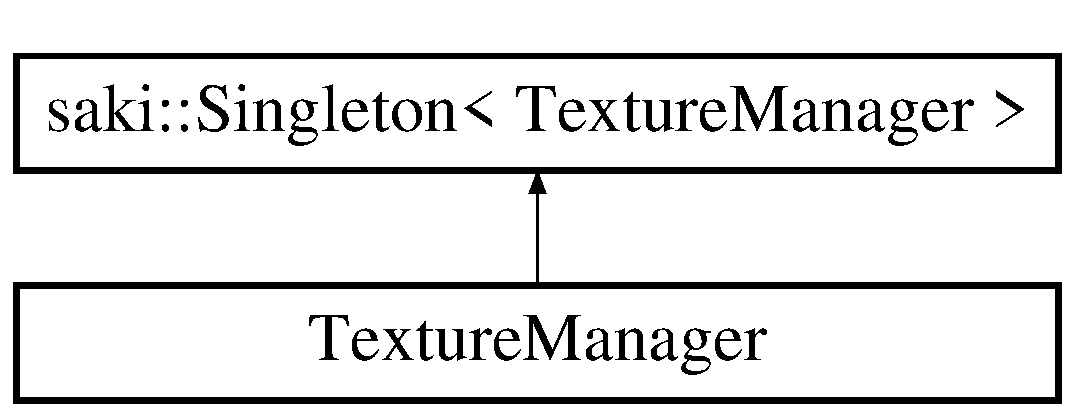
\includegraphics[height=2.000000cm]{class_texture_manager}
\end{center}
\end{figure}
\subsection*{フレンド}
\begin{DoxyCompactItemize}
\item 
class \mbox{\hyperlink{class_texture_manager_af7f909106d08e36cd50aa58e36f9bf47}{Texture}}
\end{DoxyCompactItemize}
\subsection*{その他の継承メンバ}


\subsection{フレンドと関連関数の詳解}
\mbox{\Hypertarget{class_texture_manager_af7f909106d08e36cd50aa58e36f9bf47}\label{class_texture_manager_af7f909106d08e36cd50aa58e36f9bf47}} 
\index{Texture\+Manager@{Texture\+Manager}!Texture@{Texture}}
\index{Texture@{Texture}!Texture\+Manager@{Texture\+Manager}}
\subsubsection{\texorpdfstring{Texture}{Texture}}
{\footnotesize\ttfamily friend class \mbox{\hyperlink{class_texture}{Texture}}\hspace{0.3cm}{\ttfamily [friend]}}



このクラス詳解は次のファイルから抽出されました\+:\begin{DoxyCompactItemize}
\item 
C\+:/\+Users/tokir/\+Documents/\+Git\+Hub/\+Weapon\+Merchant\+Adventure/src/src/texture/manager/\mbox{\hyperlink{texture__manager_8h}{texture\+\_\+manager.\+h}}\item 
C\+:/\+Users/tokir/\+Documents/\+Git\+Hub/\+Weapon\+Merchant\+Adventure/src/src/texture/manager/\mbox{\hyperlink{texture__manager_8cpp}{texture\+\_\+manager.\+cpp}}\end{DoxyCompactItemize}

\hypertarget{class_title_scene}{}\section{Title\+Scene クラス}
\label{class_title_scene}\index{Title\+Scene@{Title\+Scene}}


タイトルシーンクラス  




{\ttfamily \#include $<$title\+\_\+scene.\+h$>$}

Title\+Scene の継承関係図\begin{figure}[H]
\begin{center}
\leavevmode
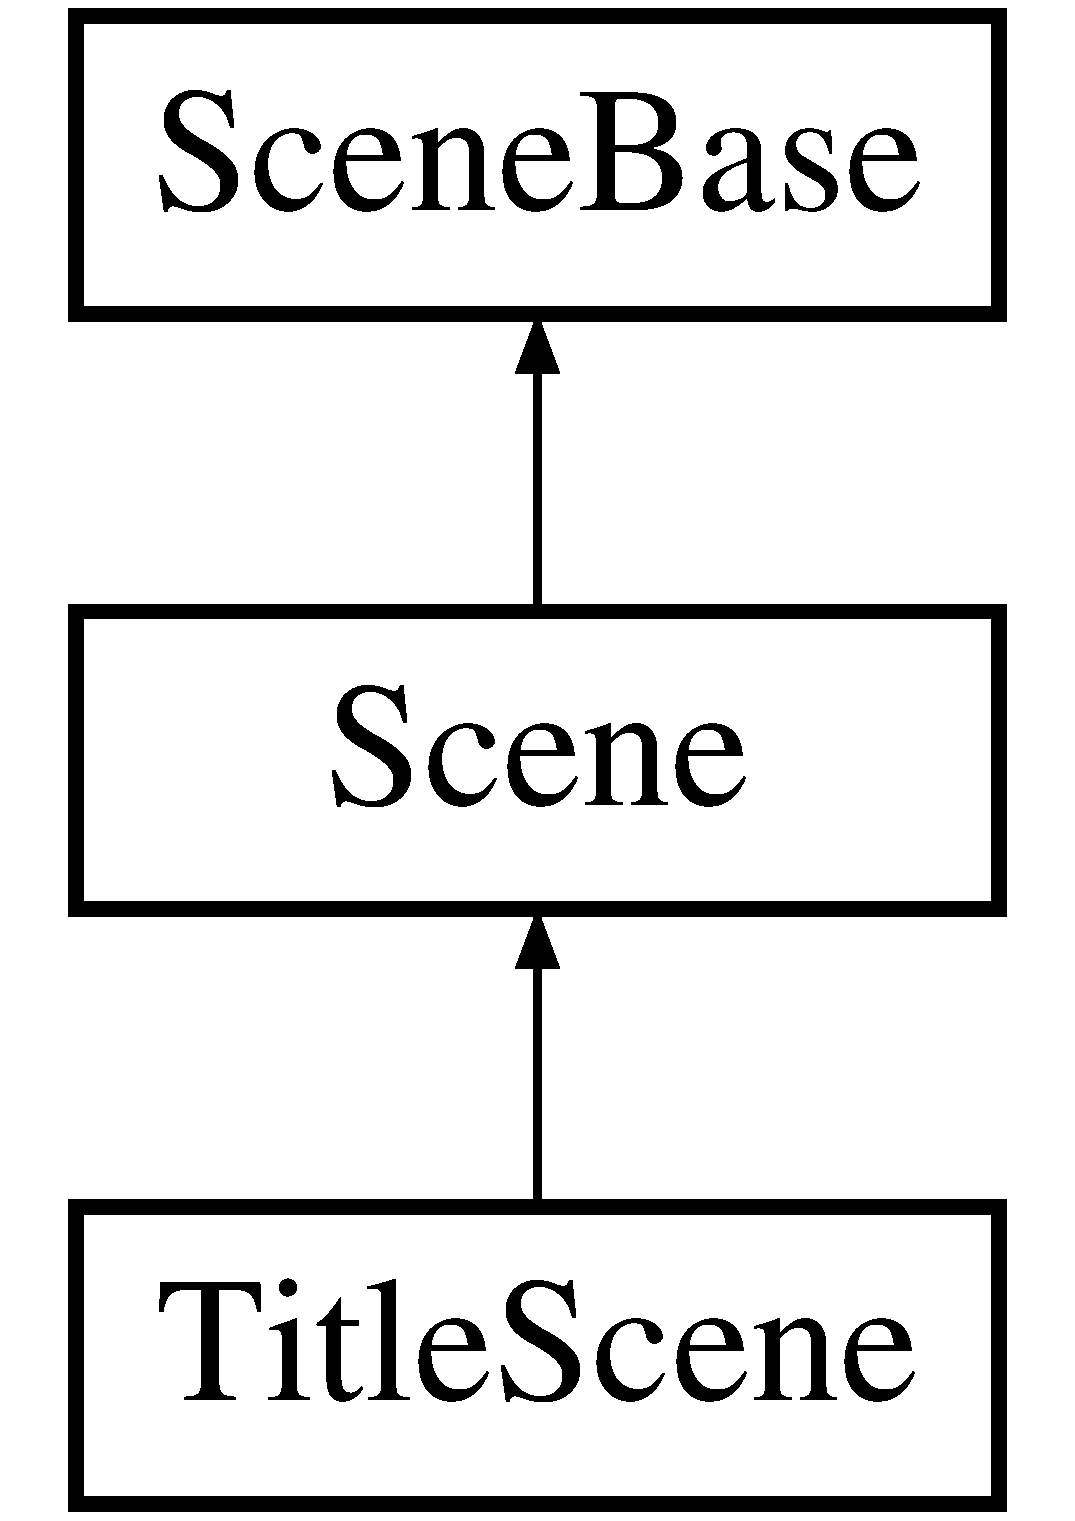
\includegraphics[height=3.000000cm]{class_title_scene}
\end{center}
\end{figure}
\subsection*{公開メンバ関数}
\begin{DoxyCompactItemize}
\item 
void \mbox{\hyperlink{class_title_scene_a3d039e7db0fa1e22e8c36d3cedfbd318}{Init}} () final
\begin{DoxyCompactList}\small\item\em タイトルシーンの初期化 \end{DoxyCompactList}\item 
\mbox{\hyperlink{scene__base_8h_a24cee5343fb9d0706ead6e8601f363be}{S\+C\+E\+NE}} \mbox{\hyperlink{class_title_scene_a19f6ee49ca6c8526fb1af2c0a2df9a33}{Update}} () final
\begin{DoxyCompactList}\small\item\em タイトルシーンの更新 \end{DoxyCompactList}\item 
void \mbox{\hyperlink{class_title_scene_af12c59b3bf9458640938c5ca620527ae}{Render}} () final
\begin{DoxyCompactList}\small\item\em タイトルシーンの描画 \end{DoxyCompactList}\item 
void \mbox{\hyperlink{class_title_scene_adfbc5f934572ede2e36419b089c88fe8}{Destroy}} () final
\begin{DoxyCompactList}\small\item\em タイトルシーンの破棄 \end{DoxyCompactList}\end{DoxyCompactItemize}
\subsection*{その他の継承メンバ}


\subsection{詳解}
タイトルシーンクラス 

\subsection{関数詳解}
\mbox{\Hypertarget{class_title_scene_adfbc5f934572ede2e36419b089c88fe8}\label{class_title_scene_adfbc5f934572ede2e36419b089c88fe8}} 
\index{Title\+Scene@{Title\+Scene}!Destroy@{Destroy}}
\index{Destroy@{Destroy}!Title\+Scene@{Title\+Scene}}
\subsubsection{\texorpdfstring{Destroy()}{Destroy()}}
{\footnotesize\ttfamily void Title\+Scene\+::\+Destroy (\begin{DoxyParamCaption}{ }\end{DoxyParamCaption})\hspace{0.3cm}{\ttfamily [final]}, {\ttfamily [virtual]}}



タイトルシーンの破棄 



\mbox{\hyperlink{class_scene_base_a7c5b54020bc519b4dadfe9770d6b27f7}{Scene\+Base}}を実装しています。

\mbox{\Hypertarget{class_title_scene_a3d039e7db0fa1e22e8c36d3cedfbd318}\label{class_title_scene_a3d039e7db0fa1e22e8c36d3cedfbd318}} 
\index{Title\+Scene@{Title\+Scene}!Init@{Init}}
\index{Init@{Init}!Title\+Scene@{Title\+Scene}}
\subsubsection{\texorpdfstring{Init()}{Init()}}
{\footnotesize\ttfamily void Title\+Scene\+::\+Init (\begin{DoxyParamCaption}{ }\end{DoxyParamCaption})\hspace{0.3cm}{\ttfamily [final]}, {\ttfamily [virtual]}}



タイトルシーンの初期化 



\mbox{\hyperlink{class_scene_base_a24d7db43c819924dc8b07b436f6d3148}{Scene\+Base}}を実装しています。

\mbox{\Hypertarget{class_title_scene_af12c59b3bf9458640938c5ca620527ae}\label{class_title_scene_af12c59b3bf9458640938c5ca620527ae}} 
\index{Title\+Scene@{Title\+Scene}!Render@{Render}}
\index{Render@{Render}!Title\+Scene@{Title\+Scene}}
\subsubsection{\texorpdfstring{Render()}{Render()}}
{\footnotesize\ttfamily void Title\+Scene\+::\+Render (\begin{DoxyParamCaption}{ }\end{DoxyParamCaption})\hspace{0.3cm}{\ttfamily [final]}, {\ttfamily [virtual]}}



タイトルシーンの描画 



\mbox{\hyperlink{class_scene_base_ad981674ce731ea267f398e889bbb9dc3}{Scene\+Base}}を実装しています。

\mbox{\Hypertarget{class_title_scene_a19f6ee49ca6c8526fb1af2c0a2df9a33}\label{class_title_scene_a19f6ee49ca6c8526fb1af2c0a2df9a33}} 
\index{Title\+Scene@{Title\+Scene}!Update@{Update}}
\index{Update@{Update}!Title\+Scene@{Title\+Scene}}
\subsubsection{\texorpdfstring{Update()}{Update()}}
{\footnotesize\ttfamily \mbox{\hyperlink{scene__base_8h_a24cee5343fb9d0706ead6e8601f363be}{S\+C\+E\+NE}} Title\+Scene\+::\+Update (\begin{DoxyParamCaption}{ }\end{DoxyParamCaption})\hspace{0.3cm}{\ttfamily [final]}, {\ttfamily [virtual]}}



タイトルシーンの更新 

\begin{DoxyReturn}{戻り値}
S\+C\+E\+NE シーンが変わるなら次のシーンのenum classを返す 
\end{DoxyReturn}


\mbox{\hyperlink{class_scene_acb50f8104e5a7cfecbdececa7d5f1b39}{Scene}}を実装しています。



このクラス詳解は次のファイルから抽出されました\+:\begin{DoxyCompactItemize}
\item 
C\+:/\+Users/tokir/\+Documents/\+Git\+Hub/\+Weapon\+Merchant\+Adventure/src/scene/main/title/\mbox{\hyperlink{title__scene_8h}{title\+\_\+scene.\+h}}\item 
C\+:/\+Users/tokir/\+Documents/\+Git\+Hub/\+Weapon\+Merchant\+Adventure/src/scene/main/title/\mbox{\hyperlink{title__scene_8cpp}{title\+\_\+scene.\+cpp}}\end{DoxyCompactItemize}

\hypertarget{classsaki_1_1_transform}{}\section{saki\+:\+:Transform$<$ T $>$ クラステンプレート}
\label{classsaki_1_1_transform}\index{saki\+::\+Transform$<$ T $>$@{saki\+::\+Transform$<$ T $>$}}


transformクラス  




{\ttfamily \#include $<$transform\+\_\+operator.\+h$>$}

\subsection*{公開メンバ関数}
\begin{DoxyCompactItemize}
\item 
constexpr \mbox{\hyperlink{classsaki_1_1_transform_abdd7b5f310bccc56b804a2cf21890a35}{Transform}} ()
\begin{DoxyCompactList}\small\item\em 引数なしコンストラクタ \end{DoxyCompactList}\item 
constexpr \mbox{\hyperlink{classsaki_1_1_transform_ad0081402f944d173d0a1df40762d571c}{Transform}} (const \mbox{\hyperlink{classsaki_1_1_vector3}{Vector3}}$<$ T $>$ \&pos, const \mbox{\hyperlink{classsaki_1_1_vector3}{Vector3}}$<$ T $>$ rot, const \mbox{\hyperlink{classsaki_1_1_vector3}{Vector3}}$<$ T $>$sca)
\begin{DoxyCompactList}\small\item\em 各値を引数にとるコンストラクタ \end{DoxyCompactList}\item 
\mbox{\hyperlink{classsaki_1_1_transform_a86e4e6b8c8a3387f5659e71b377a9995}{Transform}} (const \mbox{\hyperlink{classsaki_1_1_transform}{Transform}}$<$ T $>$ \&)=default
\item 
\mbox{\hyperlink{classsaki_1_1_transform}{Transform}}$<$ T $>$ \& \mbox{\hyperlink{classsaki_1_1_transform_acfdf423e01196edf631f272400645cfa}{operator=}} (const \mbox{\hyperlink{classsaki_1_1_transform}{Transform}}$<$ T $>$ \&)=default
\item 
\mbox{\hyperlink{classsaki_1_1_transform_a065323d290c8c4edd76855e7b9634ab8}{Transform}} (\mbox{\hyperlink{classsaki_1_1_transform}{Transform}}$<$ T $>$ \&\&)=default
\item 
\mbox{\hyperlink{classsaki_1_1_transform}{Transform}}$<$ T $>$ \& \mbox{\hyperlink{classsaki_1_1_transform_a66ea10234a845d96e63bbb9c2a1050eb}{operator=}} (\mbox{\hyperlink{classsaki_1_1_transform}{Transform}}$<$ T $>$ \&\&)=default
\item 
void \mbox{\hyperlink{classsaki_1_1_transform_a1c0f7ad966d8f4d014e6f023943bbfb7}{move}} (const \mbox{\hyperlink{classsaki_1_1_vector3}{Vector3}}$<$ T $>$ \&pos)
\begin{DoxyCompactList}\small\item\em 移動 \end{DoxyCompactList}\item 
void \mbox{\hyperlink{classsaki_1_1_transform_aa46a720684261bebf4305724817ac053}{rotate}} (const \mbox{\hyperlink{classsaki_1_1_vector3}{Vector3}}$<$ T $>$ \&rot)
\begin{DoxyCompactList}\small\item\em 回転 \end{DoxyCompactList}\item 
void \mbox{\hyperlink{classsaki_1_1_transform_a58885f17529b9c32308ec826d67a82fd}{expantion}} (const \mbox{\hyperlink{classsaki_1_1_vector3}{Vector3}}$<$ T $>$ \&sca)
\begin{DoxyCompactList}\small\item\em 拡大 \end{DoxyCompactList}\item 
auto \mbox{\hyperlink{classsaki_1_1_transform_a781a14da529aa0a45d4cfb66768ffc8c}{get\+\_\+pos}} () const
\begin{DoxyCompactList}\small\item\em 位置のゲッタ \end{DoxyCompactList}\item 
void \mbox{\hyperlink{classsaki_1_1_transform_a2659fe0773c0b8137b3a321859c3906e}{set\+\_\+pos}} (const \mbox{\hyperlink{classsaki_1_1_vector3}{Vector3}}$<$ T $>$ \&pos)
\begin{DoxyCompactList}\small\item\em 位置のセッタ \end{DoxyCompactList}\item 
auto \mbox{\hyperlink{classsaki_1_1_transform_ab5a091567c4f9f3040c0f843156d8bce}{get\+\_\+rot}} () const
\begin{DoxyCompactList}\small\item\em 回転のゲッタ \end{DoxyCompactList}\item 
void \mbox{\hyperlink{classsaki_1_1_transform_a7b30f864722819b8be85ecbd4dde43a4}{set\+\_\+rot}} (const \mbox{\hyperlink{classsaki_1_1_vector3}{Vector3}}$<$ T $>$ \&rot)
\begin{DoxyCompactList}\small\item\em 回転のセッタ \end{DoxyCompactList}\item 
auto \mbox{\hyperlink{classsaki_1_1_transform_a0ec8a9193bf5b987a72ed732b8976cfb}{get\+\_\+scale}} () const
\begin{DoxyCompactList}\small\item\em 拡縮のゲッタ \end{DoxyCompactList}\item 
void \mbox{\hyperlink{classsaki_1_1_transform_aade1855d64e42635e8b613aa055aa6fc}{set\+\_\+scale}} (const \mbox{\hyperlink{classsaki_1_1_vector3}{Vector3}}$<$ T $>$ \&sca)
\begin{DoxyCompactList}\small\item\em 拡縮のセッタ \end{DoxyCompactList}\item 
{\footnotesize template$<$typename U  = T$>$ }\\auto \mbox{\hyperlink{classsaki_1_1_transform_ae61e16c754492653881275f3942efb29}{operator+=}} (const \mbox{\hyperlink{classsaki_1_1_transform}{Transform}}$<$ U $>$ \&other)
\begin{DoxyCompactList}\small\item\em +=演算子 \end{DoxyCompactList}\item 
{\footnotesize template$<$typename U  = T$>$ }\\auto \mbox{\hyperlink{classsaki_1_1_transform_a27f9b6f3571fb0a44ca36ef51080a1d3}{operator-\/=}} (const \mbox{\hyperlink{classsaki_1_1_transform}{Transform}}$<$ U $>$ \&other)
\begin{DoxyCompactList}\small\item\em -\/=演算子 \end{DoxyCompactList}\item 
{\footnotesize template$<$typename U  = T$>$ }\\auto \mbox{\hyperlink{classsaki_1_1_transform_ab8df7cf8619c1f245d871e4e7627bf78}{operator$\ast$=}} (const U \&scalar)
\begin{DoxyCompactList}\small\item\em $\ast$=演算子(スカラ) \end{DoxyCompactList}\item 
{\footnotesize template$<$typename U  = T$>$ }\\auto \mbox{\hyperlink{classsaki_1_1_transform_a9a5559fdf626c8ecec063db74c6f4f8e}{operator/=}} (const U \&scalar)
\begin{DoxyCompactList}\small\item\em /= 演算子(スカラ) \end{DoxyCompactList}\item 
constexpr \mbox{\hyperlink{classsaki_1_1_transform}{Transform}}$<$ T $>$ \mbox{\hyperlink{classsaki_1_1_transform_a52201fc4aed19cc0459dc4b3c21c3d37}{operator+}} () const
\begin{DoxyCompactList}\small\item\em 単項+演算子 \end{DoxyCompactList}\item 
constexpr \mbox{\hyperlink{classsaki_1_1_transform}{Transform}}$<$ T $>$ \mbox{\hyperlink{classsaki_1_1_transform_a813e5118f0a23213b21a6b7f101a4584}{operator-\/}} () const
\begin{DoxyCompactList}\small\item\em 単項-\/演算子 \end{DoxyCompactList}\end{DoxyCompactItemize}


\subsection{詳解}
\subsubsection*{template$<$typename T$>$\newline
class saki\+::\+Transform$<$ T $>$}

transformクラス 

クォータニオンは使用していません 

\subsection{構築子と解体子}
\mbox{\Hypertarget{classsaki_1_1_transform_abdd7b5f310bccc56b804a2cf21890a35}\label{classsaki_1_1_transform_abdd7b5f310bccc56b804a2cf21890a35}} 
\index{saki\+::\+Transform@{saki\+::\+Transform}!Transform@{Transform}}
\index{Transform@{Transform}!saki\+::\+Transform@{saki\+::\+Transform}}
\subsubsection{\texorpdfstring{Transform()}{Transform()}\hspace{0.1cm}{\footnotesize\ttfamily [1/4]}}
{\footnotesize\ttfamily template$<$typename T$>$ \\
constexpr \mbox{\hyperlink{classsaki_1_1_transform}{saki\+::\+Transform}}$<$ T $>$\+::\mbox{\hyperlink{classsaki_1_1_transform}{Transform}} (\begin{DoxyParamCaption}{ }\end{DoxyParamCaption})\hspace{0.3cm}{\ttfamily [inline]}}



引数なしコンストラクタ 

\mbox{\Hypertarget{classsaki_1_1_transform_ad0081402f944d173d0a1df40762d571c}\label{classsaki_1_1_transform_ad0081402f944d173d0a1df40762d571c}} 
\index{saki\+::\+Transform@{saki\+::\+Transform}!Transform@{Transform}}
\index{Transform@{Transform}!saki\+::\+Transform@{saki\+::\+Transform}}
\subsubsection{\texorpdfstring{Transform()}{Transform()}\hspace{0.1cm}{\footnotesize\ttfamily [2/4]}}
{\footnotesize\ttfamily template$<$typename T$>$ \\
constexpr \mbox{\hyperlink{classsaki_1_1_transform}{saki\+::\+Transform}}$<$ T $>$\+::\mbox{\hyperlink{classsaki_1_1_transform}{Transform}} (\begin{DoxyParamCaption}\item[{const \mbox{\hyperlink{classsaki_1_1_vector3}{Vector3}}$<$ T $>$ \&}]{pos,  }\item[{const \mbox{\hyperlink{classsaki_1_1_vector3}{Vector3}}$<$ T $>$}]{rot,  }\item[{const \mbox{\hyperlink{classsaki_1_1_vector3}{Vector3}}$<$ T $>$}]{sca }\end{DoxyParamCaption})\hspace{0.3cm}{\ttfamily [inline]}}



各値を引数にとるコンストラクタ 


\begin{DoxyParams}{引数}
{\em pos} & 位置 \\
\hline
{\em rot} & 回転 \\
\hline
{\em sca} & 拡縮 \\
\hline
\end{DoxyParams}
\mbox{\Hypertarget{classsaki_1_1_transform_a86e4e6b8c8a3387f5659e71b377a9995}\label{classsaki_1_1_transform_a86e4e6b8c8a3387f5659e71b377a9995}} 
\index{saki\+::\+Transform@{saki\+::\+Transform}!Transform@{Transform}}
\index{Transform@{Transform}!saki\+::\+Transform@{saki\+::\+Transform}}
\subsubsection{\texorpdfstring{Transform()}{Transform()}\hspace{0.1cm}{\footnotesize\ttfamily [3/4]}}
{\footnotesize\ttfamily template$<$typename T$>$ \\
\mbox{\hyperlink{classsaki_1_1_transform}{saki\+::\+Transform}}$<$ T $>$\+::\mbox{\hyperlink{classsaki_1_1_transform}{Transform}} (\begin{DoxyParamCaption}\item[{const \mbox{\hyperlink{classsaki_1_1_transform}{Transform}}$<$ T $>$ \&}]{ }\end{DoxyParamCaption})\hspace{0.3cm}{\ttfamily [default]}}

\mbox{\Hypertarget{classsaki_1_1_transform_a065323d290c8c4edd76855e7b9634ab8}\label{classsaki_1_1_transform_a065323d290c8c4edd76855e7b9634ab8}} 
\index{saki\+::\+Transform@{saki\+::\+Transform}!Transform@{Transform}}
\index{Transform@{Transform}!saki\+::\+Transform@{saki\+::\+Transform}}
\subsubsection{\texorpdfstring{Transform()}{Transform()}\hspace{0.1cm}{\footnotesize\ttfamily [4/4]}}
{\footnotesize\ttfamily template$<$typename T$>$ \\
\mbox{\hyperlink{classsaki_1_1_transform}{saki\+::\+Transform}}$<$ T $>$\+::\mbox{\hyperlink{classsaki_1_1_transform}{Transform}} (\begin{DoxyParamCaption}\item[{\mbox{\hyperlink{classsaki_1_1_transform}{Transform}}$<$ T $>$ \&\&}]{ }\end{DoxyParamCaption})\hspace{0.3cm}{\ttfamily [default]}}



\subsection{関数詳解}
\mbox{\Hypertarget{classsaki_1_1_transform_a58885f17529b9c32308ec826d67a82fd}\label{classsaki_1_1_transform_a58885f17529b9c32308ec826d67a82fd}} 
\index{saki\+::\+Transform@{saki\+::\+Transform}!expantion@{expantion}}
\index{expantion@{expantion}!saki\+::\+Transform@{saki\+::\+Transform}}
\subsubsection{\texorpdfstring{expantion()}{expantion()}}
{\footnotesize\ttfamily template$<$typename T$>$ \\
void \mbox{\hyperlink{classsaki_1_1_transform}{saki\+::\+Transform}}$<$ T $>$\+::expantion (\begin{DoxyParamCaption}\item[{const \mbox{\hyperlink{classsaki_1_1_vector3}{Vector3}}$<$ T $>$ \&}]{sca }\end{DoxyParamCaption})\hspace{0.3cm}{\ttfamily [inline]}}



拡大 

\mbox{\Hypertarget{classsaki_1_1_transform_a781a14da529aa0a45d4cfb66768ffc8c}\label{classsaki_1_1_transform_a781a14da529aa0a45d4cfb66768ffc8c}} 
\index{saki\+::\+Transform@{saki\+::\+Transform}!get\+\_\+pos@{get\+\_\+pos}}
\index{get\+\_\+pos@{get\+\_\+pos}!saki\+::\+Transform@{saki\+::\+Transform}}
\subsubsection{\texorpdfstring{get\+\_\+pos()}{get\_pos()}}
{\footnotesize\ttfamily template$<$typename T$>$ \\
auto \mbox{\hyperlink{classsaki_1_1_transform}{saki\+::\+Transform}}$<$ T $>$\+::get\+\_\+pos (\begin{DoxyParamCaption}{ }\end{DoxyParamCaption}) const\hspace{0.3cm}{\ttfamily [inline]}}



位置のゲッタ 

\mbox{\Hypertarget{classsaki_1_1_transform_ab5a091567c4f9f3040c0f843156d8bce}\label{classsaki_1_1_transform_ab5a091567c4f9f3040c0f843156d8bce}} 
\index{saki\+::\+Transform@{saki\+::\+Transform}!get\+\_\+rot@{get\+\_\+rot}}
\index{get\+\_\+rot@{get\+\_\+rot}!saki\+::\+Transform@{saki\+::\+Transform}}
\subsubsection{\texorpdfstring{get\+\_\+rot()}{get\_rot()}}
{\footnotesize\ttfamily template$<$typename T$>$ \\
auto \mbox{\hyperlink{classsaki_1_1_transform}{saki\+::\+Transform}}$<$ T $>$\+::get\+\_\+rot (\begin{DoxyParamCaption}{ }\end{DoxyParamCaption}) const\hspace{0.3cm}{\ttfamily [inline]}}



回転のゲッタ 

\mbox{\Hypertarget{classsaki_1_1_transform_a0ec8a9193bf5b987a72ed732b8976cfb}\label{classsaki_1_1_transform_a0ec8a9193bf5b987a72ed732b8976cfb}} 
\index{saki\+::\+Transform@{saki\+::\+Transform}!get\+\_\+scale@{get\+\_\+scale}}
\index{get\+\_\+scale@{get\+\_\+scale}!saki\+::\+Transform@{saki\+::\+Transform}}
\subsubsection{\texorpdfstring{get\+\_\+scale()}{get\_scale()}}
{\footnotesize\ttfamily template$<$typename T$>$ \\
auto \mbox{\hyperlink{classsaki_1_1_transform}{saki\+::\+Transform}}$<$ T $>$\+::get\+\_\+scale (\begin{DoxyParamCaption}{ }\end{DoxyParamCaption}) const\hspace{0.3cm}{\ttfamily [inline]}}



拡縮のゲッタ 

\mbox{\Hypertarget{classsaki_1_1_transform_a1c0f7ad966d8f4d014e6f023943bbfb7}\label{classsaki_1_1_transform_a1c0f7ad966d8f4d014e6f023943bbfb7}} 
\index{saki\+::\+Transform@{saki\+::\+Transform}!move@{move}}
\index{move@{move}!saki\+::\+Transform@{saki\+::\+Transform}}
\subsubsection{\texorpdfstring{move()}{move()}}
{\footnotesize\ttfamily template$<$typename T$>$ \\
void \mbox{\hyperlink{classsaki_1_1_transform}{saki\+::\+Transform}}$<$ T $>$\+::move (\begin{DoxyParamCaption}\item[{const \mbox{\hyperlink{classsaki_1_1_vector3}{Vector3}}$<$ T $>$ \&}]{pos }\end{DoxyParamCaption})\hspace{0.3cm}{\ttfamily [inline]}}



移動 

\mbox{\Hypertarget{classsaki_1_1_transform_ab8df7cf8619c1f245d871e4e7627bf78}\label{classsaki_1_1_transform_ab8df7cf8619c1f245d871e4e7627bf78}} 
\index{saki\+::\+Transform@{saki\+::\+Transform}!operator$\ast$=@{operator$\ast$=}}
\index{operator$\ast$=@{operator$\ast$=}!saki\+::\+Transform@{saki\+::\+Transform}}
\subsubsection{\texorpdfstring{operator$\ast$=()}{operator*=()}}
{\footnotesize\ttfamily template$<$typename T$>$ \\
template$<$typename U  = T$>$ \\
auto \mbox{\hyperlink{classsaki_1_1_transform}{saki\+::\+Transform}}$<$ T $>$\+::operator$\ast$= (\begin{DoxyParamCaption}\item[{const U \&}]{scalar }\end{DoxyParamCaption})\hspace{0.3cm}{\ttfamily [inline]}}



$\ast$=演算子(スカラ) 

\mbox{\Hypertarget{classsaki_1_1_transform_a52201fc4aed19cc0459dc4b3c21c3d37}\label{classsaki_1_1_transform_a52201fc4aed19cc0459dc4b3c21c3d37}} 
\index{saki\+::\+Transform@{saki\+::\+Transform}!operator+@{operator+}}
\index{operator+@{operator+}!saki\+::\+Transform@{saki\+::\+Transform}}
\subsubsection{\texorpdfstring{operator+()}{operator+()}}
{\footnotesize\ttfamily template$<$typename T$>$ \\
constexpr \mbox{\hyperlink{classsaki_1_1_transform}{Transform}}$<$T$>$ \mbox{\hyperlink{classsaki_1_1_transform}{saki\+::\+Transform}}$<$ T $>$\+::operator+ (\begin{DoxyParamCaption}{ }\end{DoxyParamCaption}) const\hspace{0.3cm}{\ttfamily [inline]}}



単項+演算子 

\mbox{\Hypertarget{classsaki_1_1_transform_ae61e16c754492653881275f3942efb29}\label{classsaki_1_1_transform_ae61e16c754492653881275f3942efb29}} 
\index{saki\+::\+Transform@{saki\+::\+Transform}!operator+=@{operator+=}}
\index{operator+=@{operator+=}!saki\+::\+Transform@{saki\+::\+Transform}}
\subsubsection{\texorpdfstring{operator+=()}{operator+=()}}
{\footnotesize\ttfamily template$<$typename T$>$ \\
template$<$typename U  = T$>$ \\
auto \mbox{\hyperlink{classsaki_1_1_transform}{saki\+::\+Transform}}$<$ T $>$\+::operator+= (\begin{DoxyParamCaption}\item[{const \mbox{\hyperlink{classsaki_1_1_transform}{Transform}}$<$ U $>$ \&}]{other }\end{DoxyParamCaption})\hspace{0.3cm}{\ttfamily [inline]}}



+=演算子 

\mbox{\Hypertarget{classsaki_1_1_transform_a813e5118f0a23213b21a6b7f101a4584}\label{classsaki_1_1_transform_a813e5118f0a23213b21a6b7f101a4584}} 
\index{saki\+::\+Transform@{saki\+::\+Transform}!operator-\/@{operator-\/}}
\index{operator-\/@{operator-\/}!saki\+::\+Transform@{saki\+::\+Transform}}
\subsubsection{\texorpdfstring{operator-\/()}{operator-()}}
{\footnotesize\ttfamily template$<$typename T$>$ \\
constexpr \mbox{\hyperlink{classsaki_1_1_transform}{Transform}}$<$T$>$ \mbox{\hyperlink{classsaki_1_1_transform}{saki\+::\+Transform}}$<$ T $>$\+::operator-\/ (\begin{DoxyParamCaption}{ }\end{DoxyParamCaption}) const\hspace{0.3cm}{\ttfamily [inline]}}



単項-\/演算子 

\mbox{\Hypertarget{classsaki_1_1_transform_a27f9b6f3571fb0a44ca36ef51080a1d3}\label{classsaki_1_1_transform_a27f9b6f3571fb0a44ca36ef51080a1d3}} 
\index{saki\+::\+Transform@{saki\+::\+Transform}!operator-\/=@{operator-\/=}}
\index{operator-\/=@{operator-\/=}!saki\+::\+Transform@{saki\+::\+Transform}}
\subsubsection{\texorpdfstring{operator-\/=()}{operator-=()}}
{\footnotesize\ttfamily template$<$typename T$>$ \\
template$<$typename U  = T$>$ \\
auto \mbox{\hyperlink{classsaki_1_1_transform}{saki\+::\+Transform}}$<$ T $>$\+::operator-\/= (\begin{DoxyParamCaption}\item[{const \mbox{\hyperlink{classsaki_1_1_transform}{Transform}}$<$ U $>$ \&}]{other }\end{DoxyParamCaption})\hspace{0.3cm}{\ttfamily [inline]}}



-\/=演算子 

\mbox{\Hypertarget{classsaki_1_1_transform_a9a5559fdf626c8ecec063db74c6f4f8e}\label{classsaki_1_1_transform_a9a5559fdf626c8ecec063db74c6f4f8e}} 
\index{saki\+::\+Transform@{saki\+::\+Transform}!operator/=@{operator/=}}
\index{operator/=@{operator/=}!saki\+::\+Transform@{saki\+::\+Transform}}
\subsubsection{\texorpdfstring{operator/=()}{operator/=()}}
{\footnotesize\ttfamily template$<$typename T$>$ \\
template$<$typename U  = T$>$ \\
auto \mbox{\hyperlink{classsaki_1_1_transform}{saki\+::\+Transform}}$<$ T $>$\+::operator/= (\begin{DoxyParamCaption}\item[{const U \&}]{scalar }\end{DoxyParamCaption})\hspace{0.3cm}{\ttfamily [inline]}}



/= 演算子(スカラ) 

\mbox{\Hypertarget{classsaki_1_1_transform_acfdf423e01196edf631f272400645cfa}\label{classsaki_1_1_transform_acfdf423e01196edf631f272400645cfa}} 
\index{saki\+::\+Transform@{saki\+::\+Transform}!operator=@{operator=}}
\index{operator=@{operator=}!saki\+::\+Transform@{saki\+::\+Transform}}
\subsubsection{\texorpdfstring{operator=()}{operator=()}\hspace{0.1cm}{\footnotesize\ttfamily [1/2]}}
{\footnotesize\ttfamily template$<$typename T$>$ \\
\mbox{\hyperlink{classsaki_1_1_transform}{Transform}}$<$T$>$\& \mbox{\hyperlink{classsaki_1_1_transform}{saki\+::\+Transform}}$<$ T $>$\+::operator= (\begin{DoxyParamCaption}\item[{const \mbox{\hyperlink{classsaki_1_1_transform}{Transform}}$<$ T $>$ \&}]{ }\end{DoxyParamCaption})\hspace{0.3cm}{\ttfamily [default]}}

\mbox{\Hypertarget{classsaki_1_1_transform_a66ea10234a845d96e63bbb9c2a1050eb}\label{classsaki_1_1_transform_a66ea10234a845d96e63bbb9c2a1050eb}} 
\index{saki\+::\+Transform@{saki\+::\+Transform}!operator=@{operator=}}
\index{operator=@{operator=}!saki\+::\+Transform@{saki\+::\+Transform}}
\subsubsection{\texorpdfstring{operator=()}{operator=()}\hspace{0.1cm}{\footnotesize\ttfamily [2/2]}}
{\footnotesize\ttfamily template$<$typename T$>$ \\
\mbox{\hyperlink{classsaki_1_1_transform}{Transform}}$<$T$>$\& \mbox{\hyperlink{classsaki_1_1_transform}{saki\+::\+Transform}}$<$ T $>$\+::operator= (\begin{DoxyParamCaption}\item[{\mbox{\hyperlink{classsaki_1_1_transform}{Transform}}$<$ T $>$ \&\&}]{ }\end{DoxyParamCaption})\hspace{0.3cm}{\ttfamily [default]}}

\mbox{\Hypertarget{classsaki_1_1_transform_aa46a720684261bebf4305724817ac053}\label{classsaki_1_1_transform_aa46a720684261bebf4305724817ac053}} 
\index{saki\+::\+Transform@{saki\+::\+Transform}!rotate@{rotate}}
\index{rotate@{rotate}!saki\+::\+Transform@{saki\+::\+Transform}}
\subsubsection{\texorpdfstring{rotate()}{rotate()}}
{\footnotesize\ttfamily template$<$typename T$>$ \\
void \mbox{\hyperlink{classsaki_1_1_transform}{saki\+::\+Transform}}$<$ T $>$\+::rotate (\begin{DoxyParamCaption}\item[{const \mbox{\hyperlink{classsaki_1_1_vector3}{Vector3}}$<$ T $>$ \&}]{rot }\end{DoxyParamCaption})\hspace{0.3cm}{\ttfamily [inline]}}



回転 

\mbox{\Hypertarget{classsaki_1_1_transform_a2659fe0773c0b8137b3a321859c3906e}\label{classsaki_1_1_transform_a2659fe0773c0b8137b3a321859c3906e}} 
\index{saki\+::\+Transform@{saki\+::\+Transform}!set\+\_\+pos@{set\+\_\+pos}}
\index{set\+\_\+pos@{set\+\_\+pos}!saki\+::\+Transform@{saki\+::\+Transform}}
\subsubsection{\texorpdfstring{set\+\_\+pos()}{set\_pos()}}
{\footnotesize\ttfamily template$<$typename T$>$ \\
void \mbox{\hyperlink{classsaki_1_1_transform}{saki\+::\+Transform}}$<$ T $>$\+::set\+\_\+pos (\begin{DoxyParamCaption}\item[{const \mbox{\hyperlink{classsaki_1_1_vector3}{Vector3}}$<$ T $>$ \&}]{pos }\end{DoxyParamCaption})\hspace{0.3cm}{\ttfamily [inline]}}



位置のセッタ 


\begin{DoxyParams}{引数}
{\em pos} & 位置 \\
\hline
\end{DoxyParams}
\mbox{\Hypertarget{classsaki_1_1_transform_a7b30f864722819b8be85ecbd4dde43a4}\label{classsaki_1_1_transform_a7b30f864722819b8be85ecbd4dde43a4}} 
\index{saki\+::\+Transform@{saki\+::\+Transform}!set\+\_\+rot@{set\+\_\+rot}}
\index{set\+\_\+rot@{set\+\_\+rot}!saki\+::\+Transform@{saki\+::\+Transform}}
\subsubsection{\texorpdfstring{set\+\_\+rot()}{set\_rot()}}
{\footnotesize\ttfamily template$<$typename T$>$ \\
void \mbox{\hyperlink{classsaki_1_1_transform}{saki\+::\+Transform}}$<$ T $>$\+::set\+\_\+rot (\begin{DoxyParamCaption}\item[{const \mbox{\hyperlink{classsaki_1_1_vector3}{Vector3}}$<$ T $>$ \&}]{rot }\end{DoxyParamCaption})\hspace{0.3cm}{\ttfamily [inline]}}



回転のセッタ 


\begin{DoxyParams}{引数}
{\em rot} & 回転 \\
\hline
\end{DoxyParams}
\mbox{\Hypertarget{classsaki_1_1_transform_aade1855d64e42635e8b613aa055aa6fc}\label{classsaki_1_1_transform_aade1855d64e42635e8b613aa055aa6fc}} 
\index{saki\+::\+Transform@{saki\+::\+Transform}!set\+\_\+scale@{set\+\_\+scale}}
\index{set\+\_\+scale@{set\+\_\+scale}!saki\+::\+Transform@{saki\+::\+Transform}}
\subsubsection{\texorpdfstring{set\+\_\+scale()}{set\_scale()}}
{\footnotesize\ttfamily template$<$typename T$>$ \\
void \mbox{\hyperlink{classsaki_1_1_transform}{saki\+::\+Transform}}$<$ T $>$\+::set\+\_\+scale (\begin{DoxyParamCaption}\item[{const \mbox{\hyperlink{classsaki_1_1_vector3}{Vector3}}$<$ T $>$ \&}]{sca }\end{DoxyParamCaption})\hspace{0.3cm}{\ttfamily [inline]}}



拡縮のセッタ 


\begin{DoxyParams}{引数}
{\em sca} & 拡縮 \\
\hline
\end{DoxyParams}


このクラス詳解は次のファイルから抽出されました\+:\begin{DoxyCompactItemize}
\item 
C\+:/\+Users/tokir/\+Documents/\+Git\+Hub/\+Weapon\+Merchant\+Adventure/src/lib/saki/transform/details/\mbox{\hyperlink{transform__operator_8h}{transform\+\_\+operator.\+h}}\item 
C\+:/\+Users/tokir/\+Documents/\+Git\+Hub/\+Weapon\+Merchant\+Adventure/src/lib/saki/transform/\mbox{\hyperlink{transform_8h}{transform.\+h}}\end{DoxyCompactItemize}

\hypertarget{classsaki_1_1_tree}{}\section{saki\+:\+:Tree$<$ T $>$ クラステンプレート}
\label{classsaki_1_1_tree}\index{saki\+::\+Tree$<$ T $>$@{saki\+::\+Tree$<$ T $>$}}


{\ttfamily \#include $<$node.\+h$>$}

\subsection*{公開メンバ関数}
\begin{DoxyCompactItemize}
\item 
\mbox{\hyperlink{classsaki_1_1_tree_aaf7bba903c917f6ee098e5c02b75b6ec}{Tree}} ()
\begin{DoxyCompactList}\small\item\em 引数なしコンストラクタ \end{DoxyCompactList}\item 
\mbox{\hyperlink{classsaki_1_1_tree_a3b755ca793a3e3c9dd6e0aee77bf7bd6}{Tree}} (const std\+::string \&name, T t)
\begin{DoxyCompactList}\small\item\em 引数ありコンストラクタ \end{DoxyCompactList}\item 
std\+::shared\+\_\+ptr$<$ \mbox{\hyperlink{classsaki_1_1_node}{Node}}$<$ T $>$ $>$ \mbox{\hyperlink{classsaki_1_1_tree_aa0f905a290a69becb68388d7bbfd9e9f}{add\+\_\+child}} (const std\+::string \&node\+\_\+name, T t)
\begin{DoxyCompactList}\small\item\em ノードの追加 \end{DoxyCompactList}\item 
std\+::shared\+\_\+ptr$<$ \mbox{\hyperlink{classsaki_1_1_node}{Node}}$<$ T $>$ $>$ \mbox{\hyperlink{classsaki_1_1_tree_aad47033095b8e210bd2e265f7160e176}{get\+\_\+node}} (const std\+::string \&node\+\_\+path=\char`\"{}\char`\"{}) const
\begin{DoxyCompactList}\small\item\em ルートディレクトリからノードをめぐり、たどり着いたノードを返す \end{DoxyCompactList}\item 
std\+::shared\+\_\+ptr$<$ \mbox{\hyperlink{classsaki_1_1_node}{Node}}$<$ T $>$ $>$ \mbox{\hyperlink{classsaki_1_1_tree_a5ca3a3226e542530008a270ee958d6e1}{get\+\_\+root}} () const
\begin{DoxyCompactList}\small\item\em rootの取得 \end{DoxyCompactList}\item 
\mbox{\hyperlink{classsaki_1_1_tree_a3716d7484b92161bbb38c362280358c0}{Tree}} (const \mbox{\hyperlink{classsaki_1_1_tree}{Tree}} \&other)
\begin{DoxyCompactList}\small\item\em コピーコンストラクタ \end{DoxyCompactList}\item 
\mbox{\hyperlink{classsaki_1_1_tree}{Tree}}$<$ T $>$ \& \mbox{\hyperlink{classsaki_1_1_tree_ab5f73b5b7cee4f70663d03803401547b}{operator=}} (const \mbox{\hyperlink{classsaki_1_1_tree}{Tree}} \&)=default
\item 
\mbox{\hyperlink{classsaki_1_1_tree_ad26ec9d86d0ed3f360c88ea4342b726f}{Tree}} (\mbox{\hyperlink{classsaki_1_1_tree}{Tree}} \&\&other) noexcept
\item 
\mbox{\hyperlink{classsaki_1_1_tree}{Tree}}$<$ T $>$ \& \mbox{\hyperlink{classsaki_1_1_tree_a71749080c165c790b38596e5c0c151df}{operator=}} (\mbox{\hyperlink{classsaki_1_1_tree}{Tree}} \&\&) noexcept=default
\item 
void \mbox{\hyperlink{classsaki_1_1_tree_a1a2c7a0f165de86065bddd676cca6f15}{all\+\_\+node\+\_\+name}} ()
\begin{DoxyCompactList}\small\item\em デバッグ用の出力関数 \end{DoxyCompactList}\end{DoxyCompactItemize}


\subsection{構築子と解体子}
\mbox{\Hypertarget{classsaki_1_1_tree_aaf7bba903c917f6ee098e5c02b75b6ec}\label{classsaki_1_1_tree_aaf7bba903c917f6ee098e5c02b75b6ec}} 
\index{saki\+::\+Tree@{saki\+::\+Tree}!Tree@{Tree}}
\index{Tree@{Tree}!saki\+::\+Tree@{saki\+::\+Tree}}
\subsubsection{\texorpdfstring{Tree()}{Tree()}\hspace{0.1cm}{\footnotesize\ttfamily [1/4]}}
{\footnotesize\ttfamily template$<$typename T $>$ \\
\mbox{\hyperlink{classsaki_1_1_tree}{saki\+::\+Tree}}$<$ T $>$\+::\mbox{\hyperlink{classsaki_1_1_tree}{Tree}} (\begin{DoxyParamCaption}{ }\end{DoxyParamCaption})\hspace{0.3cm}{\ttfamily [inline]}}



引数なしコンストラクタ 

rootの名前はrootにする \mbox{\Hypertarget{classsaki_1_1_tree_a3b755ca793a3e3c9dd6e0aee77bf7bd6}\label{classsaki_1_1_tree_a3b755ca793a3e3c9dd6e0aee77bf7bd6}} 
\index{saki\+::\+Tree@{saki\+::\+Tree}!Tree@{Tree}}
\index{Tree@{Tree}!saki\+::\+Tree@{saki\+::\+Tree}}
\subsubsection{\texorpdfstring{Tree()}{Tree()}\hspace{0.1cm}{\footnotesize\ttfamily [2/4]}}
{\footnotesize\ttfamily template$<$typename T $>$ \\
\mbox{\hyperlink{classsaki_1_1_tree}{saki\+::\+Tree}}$<$ T $>$\+::\mbox{\hyperlink{classsaki_1_1_tree}{Tree}} (\begin{DoxyParamCaption}\item[{const std\+::string \&}]{name,  }\item[{T}]{t }\end{DoxyParamCaption})\hspace{0.3cm}{\ttfamily [inline]}}



引数ありコンストラクタ 


\begin{DoxyParams}{引数}
{\em name} & ルートノード名 \\
\hline
\end{DoxyParams}
\mbox{\Hypertarget{classsaki_1_1_tree_a3716d7484b92161bbb38c362280358c0}\label{classsaki_1_1_tree_a3716d7484b92161bbb38c362280358c0}} 
\index{saki\+::\+Tree@{saki\+::\+Tree}!Tree@{Tree}}
\index{Tree@{Tree}!saki\+::\+Tree@{saki\+::\+Tree}}
\subsubsection{\texorpdfstring{Tree()}{Tree()}\hspace{0.1cm}{\footnotesize\ttfamily [3/4]}}
{\footnotesize\ttfamily template$<$typename T $>$ \\
\mbox{\hyperlink{classsaki_1_1_tree}{saki\+::\+Tree}}$<$ T $>$\+::\mbox{\hyperlink{classsaki_1_1_tree}{Tree}} (\begin{DoxyParamCaption}\item[{const \mbox{\hyperlink{classsaki_1_1_tree}{Tree}}$<$ T $>$ \&}]{other }\end{DoxyParamCaption})\hspace{0.3cm}{\ttfamily [inline]}}



コピーコンストラクタ 

shared\+\_\+ptrを使用しているため、デフォルトコピーコンストラクタではエラーが起きる \mbox{\Hypertarget{classsaki_1_1_tree_ad26ec9d86d0ed3f360c88ea4342b726f}\label{classsaki_1_1_tree_ad26ec9d86d0ed3f360c88ea4342b726f}} 
\index{saki\+::\+Tree@{saki\+::\+Tree}!Tree@{Tree}}
\index{Tree@{Tree}!saki\+::\+Tree@{saki\+::\+Tree}}
\subsubsection{\texorpdfstring{Tree()}{Tree()}\hspace{0.1cm}{\footnotesize\ttfamily [4/4]}}
{\footnotesize\ttfamily template$<$typename T $>$ \\
\mbox{\hyperlink{classsaki_1_1_tree}{saki\+::\+Tree}}$<$ T $>$\+::\mbox{\hyperlink{classsaki_1_1_tree}{Tree}} (\begin{DoxyParamCaption}\item[{\mbox{\hyperlink{classsaki_1_1_tree}{Tree}}$<$ T $>$ \&\&}]{other }\end{DoxyParamCaption})\hspace{0.3cm}{\ttfamily [inline]}, {\ttfamily [noexcept]}}



\subsection{関数詳解}
\mbox{\Hypertarget{classsaki_1_1_tree_aa0f905a290a69becb68388d7bbfd9e9f}\label{classsaki_1_1_tree_aa0f905a290a69becb68388d7bbfd9e9f}} 
\index{saki\+::\+Tree@{saki\+::\+Tree}!add\+\_\+child@{add\+\_\+child}}
\index{add\+\_\+child@{add\+\_\+child}!saki\+::\+Tree@{saki\+::\+Tree}}
\subsubsection{\texorpdfstring{add\+\_\+child()}{add\_child()}}
{\footnotesize\ttfamily template$<$typename T $>$ \\
std\+::shared\+\_\+ptr$<$\mbox{\hyperlink{classsaki_1_1_node}{Node}}$<$T$>$ $>$ \mbox{\hyperlink{classsaki_1_1_tree}{saki\+::\+Tree}}$<$ T $>$\+::add\+\_\+child (\begin{DoxyParamCaption}\item[{const std\+::string \&}]{node\+\_\+name,  }\item[{T}]{t }\end{DoxyParamCaption})\hspace{0.3cm}{\ttfamily [inline]}}



ノードの追加 


\begin{DoxyParams}{引数}
{\em path} & パス \\
\hline
{\em node\+\_\+name} & ノード名 \\
\hline
\end{DoxyParams}
\begin{DoxyReturn}{戻り値}
ノードの追加に成功したかどうか
\end{DoxyReturn}
パスに空白を入れないでください \mbox{\Hypertarget{classsaki_1_1_tree_a1a2c7a0f165de86065bddd676cca6f15}\label{classsaki_1_1_tree_a1a2c7a0f165de86065bddd676cca6f15}} 
\index{saki\+::\+Tree@{saki\+::\+Tree}!all\+\_\+node\+\_\+name@{all\+\_\+node\+\_\+name}}
\index{all\+\_\+node\+\_\+name@{all\+\_\+node\+\_\+name}!saki\+::\+Tree@{saki\+::\+Tree}}
\subsubsection{\texorpdfstring{all\+\_\+node\+\_\+name()}{all\_node\_name()}}
{\footnotesize\ttfamily template$<$typename T $>$ \\
void \mbox{\hyperlink{classsaki_1_1_tree}{saki\+::\+Tree}}$<$ T $>$\+::all\+\_\+node\+\_\+name (\begin{DoxyParamCaption}{ }\end{DoxyParamCaption})\hspace{0.3cm}{\ttfamily [inline]}}



デバッグ用の出力関数 

\mbox{\Hypertarget{classsaki_1_1_tree_aad47033095b8e210bd2e265f7160e176}\label{classsaki_1_1_tree_aad47033095b8e210bd2e265f7160e176}} 
\index{saki\+::\+Tree@{saki\+::\+Tree}!get\+\_\+node@{get\+\_\+node}}
\index{get\+\_\+node@{get\+\_\+node}!saki\+::\+Tree@{saki\+::\+Tree}}
\subsubsection{\texorpdfstring{get\+\_\+node()}{get\_node()}}
{\footnotesize\ttfamily template$<$typename T $>$ \\
std\+::shared\+\_\+ptr$<$\mbox{\hyperlink{classsaki_1_1_node}{Node}}$<$T$>$ $>$ \mbox{\hyperlink{classsaki_1_1_tree}{saki\+::\+Tree}}$<$ T $>$\+::get\+\_\+node (\begin{DoxyParamCaption}\item[{const std\+::string \&}]{node\+\_\+path = {\ttfamily \char`\"{}\char`\"{}} }\end{DoxyParamCaption}) const\hspace{0.3cm}{\ttfamily [inline]}}



ルートディレクトリからノードをめぐり、たどり着いたノードを返す 

失敗するとrootを返す \mbox{\Hypertarget{classsaki_1_1_tree_a5ca3a3226e542530008a270ee958d6e1}\label{classsaki_1_1_tree_a5ca3a3226e542530008a270ee958d6e1}} 
\index{saki\+::\+Tree@{saki\+::\+Tree}!get\+\_\+root@{get\+\_\+root}}
\index{get\+\_\+root@{get\+\_\+root}!saki\+::\+Tree@{saki\+::\+Tree}}
\subsubsection{\texorpdfstring{get\+\_\+root()}{get\_root()}}
{\footnotesize\ttfamily template$<$typename T $>$ \\
std\+::shared\+\_\+ptr$<$\mbox{\hyperlink{classsaki_1_1_node}{Node}}$<$T$>$ $>$ \mbox{\hyperlink{classsaki_1_1_tree}{saki\+::\+Tree}}$<$ T $>$\+::get\+\_\+root (\begin{DoxyParamCaption}{ }\end{DoxyParamCaption}) const\hspace{0.3cm}{\ttfamily [inline]}}



rootの取得 

\begin{DoxyReturn}{戻り値}
root 
\end{DoxyReturn}
\mbox{\Hypertarget{classsaki_1_1_tree_ab5f73b5b7cee4f70663d03803401547b}\label{classsaki_1_1_tree_ab5f73b5b7cee4f70663d03803401547b}} 
\index{saki\+::\+Tree@{saki\+::\+Tree}!operator=@{operator=}}
\index{operator=@{operator=}!saki\+::\+Tree@{saki\+::\+Tree}}
\subsubsection{\texorpdfstring{operator=()}{operator=()}\hspace{0.1cm}{\footnotesize\ttfamily [1/2]}}
{\footnotesize\ttfamily template$<$typename T $>$ \\
\mbox{\hyperlink{classsaki_1_1_tree}{Tree}}$<$T$>$\& \mbox{\hyperlink{classsaki_1_1_tree}{saki\+::\+Tree}}$<$ T $>$\+::operator= (\begin{DoxyParamCaption}\item[{const \mbox{\hyperlink{classsaki_1_1_tree}{Tree}}$<$ T $>$ \&}]{ }\end{DoxyParamCaption})\hspace{0.3cm}{\ttfamily [default]}}

\mbox{\Hypertarget{classsaki_1_1_tree_a71749080c165c790b38596e5c0c151df}\label{classsaki_1_1_tree_a71749080c165c790b38596e5c0c151df}} 
\index{saki\+::\+Tree@{saki\+::\+Tree}!operator=@{operator=}}
\index{operator=@{operator=}!saki\+::\+Tree@{saki\+::\+Tree}}
\subsubsection{\texorpdfstring{operator=()}{operator=()}\hspace{0.1cm}{\footnotesize\ttfamily [2/2]}}
{\footnotesize\ttfamily template$<$typename T $>$ \\
\mbox{\hyperlink{classsaki_1_1_tree}{Tree}}$<$T$>$\& \mbox{\hyperlink{classsaki_1_1_tree}{saki\+::\+Tree}}$<$ T $>$\+::operator= (\begin{DoxyParamCaption}\item[{\mbox{\hyperlink{classsaki_1_1_tree}{Tree}}$<$ T $>$ \&\&}]{ }\end{DoxyParamCaption})\hspace{0.3cm}{\ttfamily [default]}, {\ttfamily [noexcept]}}



このクラス詳解は次のファイルから抽出されました\+:\begin{DoxyCompactItemize}
\item 
C\+:/\+Users/tokir/\+Documents/\+Git\+Hub/\+Weapon\+Merchant\+Adventure/src/lib/saki/tree/node/\mbox{\hyperlink{node_8h}{node.\+h}}\item 
C\+:/\+Users/tokir/\+Documents/\+Git\+Hub/\+Weapon\+Merchant\+Adventure/src/lib/saki/tree/\mbox{\hyperlink{tree_8h}{tree.\+h}}\end{DoxyCompactItemize}

\hypertarget{class_ui_image}{}\section{Ui\+Image クラス}
\label{class_ui_image}\index{Ui\+Image@{Ui\+Image}}


{\ttfamily \#include $<$ui\+\_\+image.\+h$>$}

\subsection*{公開メンバ関数}
\begin{DoxyCompactItemize}
\item 
void \mbox{\hyperlink{class_ui_image_aff0cc57cb4cf6a9edfb1fc9ce1bb8ab0}{Init}} (const std\+::string \&, W\+C\+H\+AR $\ast$, const float, const float, const \mbox{\hyperlink{common_8h_ab1cb35b3a17c398d8ef71d5f779808bf}{Vec3}} \&, const \mbox{\hyperlink{common_8h_ab1cb35b3a17c398d8ef71d5f779808bf}{Vec3}} \&, const \mbox{\hyperlink{common_8h_ab1cb35b3a17c398d8ef71d5f779808bf}{Vec3}} \&)
\item 
void \mbox{\hyperlink{class_ui_image_a2f0a08734b368e32b8cbd9f7682e0413}{Render}} ()
\item 
void \mbox{\hyperlink{class_ui_image_a2fa9658d867a9f50da24f655ae92396c}{Set\+Color}} (const float r, const float g, const float b, const float a)
\item 
void \mbox{\hyperlink{class_ui_image_a3c006a6e60e8af7c43d2548b78746e85}{Set\+Percent}} (const float percentage)
\end{DoxyCompactItemize}
\subsection*{公開変数類}
\begin{DoxyCompactItemize}
\item 
bool \mbox{\hyperlink{class_ui_image_a34d64237c00b41c32122d996c2f35f3a}{enabled}} = true
\end{DoxyCompactItemize}


\subsection{関数詳解}
\mbox{\Hypertarget{class_ui_image_aff0cc57cb4cf6a9edfb1fc9ce1bb8ab0}\label{class_ui_image_aff0cc57cb4cf6a9edfb1fc9ce1bb8ab0}} 
\index{Ui\+Image@{Ui\+Image}!Init@{Init}}
\index{Init@{Init}!Ui\+Image@{Ui\+Image}}
\subsubsection{\texorpdfstring{Init()}{Init()}}
{\footnotesize\ttfamily void Ui\+Image\+::\+Init (\begin{DoxyParamCaption}\item[{const std\+::string \&}]{name,  }\item[{W\+C\+H\+AR $\ast$}]{path,  }\item[{const float}]{w,  }\item[{const float}]{h,  }\item[{const \mbox{\hyperlink{common_8h_ab1cb35b3a17c398d8ef71d5f779808bf}{Vec3}} \&}]{pos,  }\item[{const \mbox{\hyperlink{common_8h_ab1cb35b3a17c398d8ef71d5f779808bf}{Vec3}} \&}]{rot,  }\item[{const \mbox{\hyperlink{common_8h_ab1cb35b3a17c398d8ef71d5f779808bf}{Vec3}} \&}]{scale }\end{DoxyParamCaption})}

\mbox{\Hypertarget{class_ui_image_a2f0a08734b368e32b8cbd9f7682e0413}\label{class_ui_image_a2f0a08734b368e32b8cbd9f7682e0413}} 
\index{Ui\+Image@{Ui\+Image}!Render@{Render}}
\index{Render@{Render}!Ui\+Image@{Ui\+Image}}
\subsubsection{\texorpdfstring{Render()}{Render()}}
{\footnotesize\ttfamily void Ui\+Image\+::\+Render (\begin{DoxyParamCaption}{ }\end{DoxyParamCaption})}

\mbox{\Hypertarget{class_ui_image_a2fa9658d867a9f50da24f655ae92396c}\label{class_ui_image_a2fa9658d867a9f50da24f655ae92396c}} 
\index{Ui\+Image@{Ui\+Image}!Set\+Color@{Set\+Color}}
\index{Set\+Color@{Set\+Color}!Ui\+Image@{Ui\+Image}}
\subsubsection{\texorpdfstring{Set\+Color()}{SetColor()}}
{\footnotesize\ttfamily void Ui\+Image\+::\+Set\+Color (\begin{DoxyParamCaption}\item[{const float}]{r,  }\item[{const float}]{g,  }\item[{const float}]{b,  }\item[{const float}]{a }\end{DoxyParamCaption})\hspace{0.3cm}{\ttfamily [inline]}}

\mbox{\Hypertarget{class_ui_image_a3c006a6e60e8af7c43d2548b78746e85}\label{class_ui_image_a3c006a6e60e8af7c43d2548b78746e85}} 
\index{Ui\+Image@{Ui\+Image}!Set\+Percent@{Set\+Percent}}
\index{Set\+Percent@{Set\+Percent}!Ui\+Image@{Ui\+Image}}
\subsubsection{\texorpdfstring{Set\+Percent()}{SetPercent()}}
{\footnotesize\ttfamily void Ui\+Image\+::\+Set\+Percent (\begin{DoxyParamCaption}\item[{const float}]{percentage }\end{DoxyParamCaption})\hspace{0.3cm}{\ttfamily [inline]}}



\subsection{メンバ詳解}
\mbox{\Hypertarget{class_ui_image_a34d64237c00b41c32122d996c2f35f3a}\label{class_ui_image_a34d64237c00b41c32122d996c2f35f3a}} 
\index{Ui\+Image@{Ui\+Image}!enabled@{enabled}}
\index{enabled@{enabled}!Ui\+Image@{Ui\+Image}}
\subsubsection{\texorpdfstring{enabled}{enabled}}
{\footnotesize\ttfamily bool Ui\+Image\+::enabled = true}



このクラス詳解は次のファイルから抽出されました\+:\begin{DoxyCompactItemize}
\item 
C\+:/\+Users/tokir/\+Documents/\+Git\+Hub/\+Weapon\+Merchant\+Adventure/src/src/object/ui/image/\mbox{\hyperlink{ui__image_8h}{ui\+\_\+image.\+h}}\item 
C\+:/\+Users/tokir/\+Documents/\+Git\+Hub/\+Weapon\+Merchant\+Adventure/src/src/object/ui/image/\mbox{\hyperlink{ui__image_8cpp}{ui\+\_\+image.\+cpp}}\end{DoxyCompactItemize}

\hypertarget{class_ui_manager}{}\section{Ui\+Manager クラス}
\label{class_ui_manager}\index{Ui\+Manager@{Ui\+Manager}}


{\ttfamily \#include $<$ui\+\_\+manager.\+h$>$}

Ui\+Manager の継承関係図\begin{figure}[H]
\begin{center}
\leavevmode
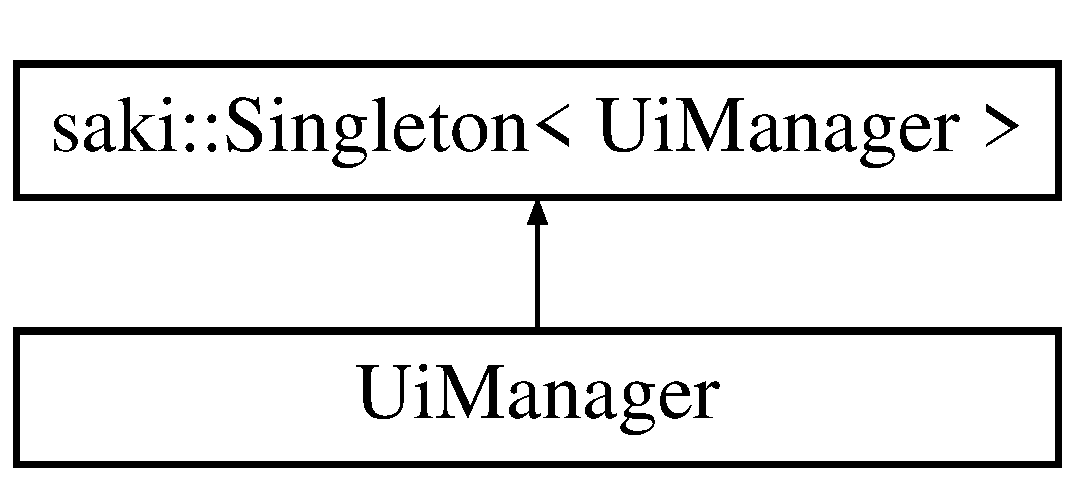
\includegraphics[height=2.000000cm]{class_ui_manager}
\end{center}
\end{figure}
\subsection*{公開メンバ関数}
\begin{DoxyCompactItemize}
\item 
void \mbox{\hyperlink{class_ui_manager_a13f50b379bf2405061d461dd427190fa}{Set\+Ui\+Image}} (\mbox{\hyperlink{class_ui_image}{Ui\+Image}} $\ast$image)
\item 
void \mbox{\hyperlink{class_ui_manager_a502cad1dd064757aea72ccf1377699b4}{Render}} ()
\item 
void \mbox{\hyperlink{class_ui_manager_ab4c659643580171b6c0db341e88e037c}{Destroy}} ()
\end{DoxyCompactItemize}
\subsection*{その他の継承メンバ}


\subsection{関数詳解}
\mbox{\Hypertarget{class_ui_manager_ab4c659643580171b6c0db341e88e037c}\label{class_ui_manager_ab4c659643580171b6c0db341e88e037c}} 
\index{Ui\+Manager@{Ui\+Manager}!Destroy@{Destroy}}
\index{Destroy@{Destroy}!Ui\+Manager@{Ui\+Manager}}
\subsubsection{\texorpdfstring{Destroy()}{Destroy()}}
{\footnotesize\ttfamily void Ui\+Manager\+::\+Destroy (\begin{DoxyParamCaption}{ }\end{DoxyParamCaption})\hspace{0.3cm}{\ttfamily [inline]}}

\mbox{\Hypertarget{class_ui_manager_a502cad1dd064757aea72ccf1377699b4}\label{class_ui_manager_a502cad1dd064757aea72ccf1377699b4}} 
\index{Ui\+Manager@{Ui\+Manager}!Render@{Render}}
\index{Render@{Render}!Ui\+Manager@{Ui\+Manager}}
\subsubsection{\texorpdfstring{Render()}{Render()}}
{\footnotesize\ttfamily void Ui\+Manager\+::\+Render (\begin{DoxyParamCaption}{ }\end{DoxyParamCaption})\hspace{0.3cm}{\ttfamily [inline]}}

\mbox{\Hypertarget{class_ui_manager_a13f50b379bf2405061d461dd427190fa}\label{class_ui_manager_a13f50b379bf2405061d461dd427190fa}} 
\index{Ui\+Manager@{Ui\+Manager}!Set\+Ui\+Image@{Set\+Ui\+Image}}
\index{Set\+Ui\+Image@{Set\+Ui\+Image}!Ui\+Manager@{Ui\+Manager}}
\subsubsection{\texorpdfstring{Set\+Ui\+Image()}{SetUiImage()}}
{\footnotesize\ttfamily void Ui\+Manager\+::\+Set\+Ui\+Image (\begin{DoxyParamCaption}\item[{\mbox{\hyperlink{class_ui_image}{Ui\+Image}} $\ast$}]{image }\end{DoxyParamCaption})\hspace{0.3cm}{\ttfamily [inline]}}



このクラス詳解は次のファイルから抽出されました\+:\begin{DoxyCompactItemize}
\item 
C\+:/\+Users/tokir/\+Documents/\+Git\+Hub/\+Weapon\+Merchant\+Adventure/src/src/object/ui/manager/\mbox{\hyperlink{ui__manager_8h}{ui\+\_\+manager.\+h}}\end{DoxyCompactItemize}

\hypertarget{classsaki_1_1_vector2}{}\section{saki\+:\+:Vector2$<$ T $>$ クラステンプレート}
\label{classsaki_1_1_vector2}\index{saki\+::\+Vector2$<$ T $>$@{saki\+::\+Vector2$<$ T $>$}}


2次元でのベクトル  




{\ttfamily \#include $<$vector\+\_\+2d\+\_\+operator.\+h$>$}

\subsection*{公開メンバ関数}
\begin{DoxyCompactItemize}
\item 
constexpr \mbox{\hyperlink{classsaki_1_1_vector2_af57b72f4255812a361bef1922a226f86}{Vector2}} ()
\begin{DoxyCompactList}\small\item\em 引数なしコンストラクタ \end{DoxyCompactList}\item 
constexpr \mbox{\hyperlink{classsaki_1_1_vector2_ad0f3d0a05370f1ef4947520245f6e9a8}{Vector2}} (const T \&\+\_\+x, const T \&\+\_\+y)
\begin{DoxyCompactList}\small\item\em 引数ありコンストラクタ \end{DoxyCompactList}\item 
constexpr \mbox{\hyperlink{classsaki_1_1_vector2_ad2c0fd66544f68066179490647244b14}{Vector2}} (const T $\ast$const pointer)
\begin{DoxyCompactList}\small\item\em 生配列からの初期化 \end{DoxyCompactList}\item 
\mbox{\hyperlink{classsaki_1_1_vector2_af3d61bb90047a8621cba0a17b265bfaa}{Vector2}} (const \mbox{\hyperlink{classsaki_1_1_vector2}{Vector2}}$<$ T $>$ \&)=default
\item 
\mbox{\hyperlink{classsaki_1_1_vector2}{Vector2}}$<$ T $>$ \& \mbox{\hyperlink{classsaki_1_1_vector2_ae6ee2a6387bfe58bdd5bf74d388370a9}{operator=}} (const \mbox{\hyperlink{classsaki_1_1_vector2}{Vector2}}$<$ T $>$ \&)=default
\item 
\mbox{\hyperlink{classsaki_1_1_vector2_ade059efe536b29346642aacbd973d062}{Vector2}} (\mbox{\hyperlink{classsaki_1_1_vector2}{Vector2}}$<$ T $>$ \&\&) noexcept=default
\item 
\mbox{\hyperlink{classsaki_1_1_vector2}{Vector2}} \& \mbox{\hyperlink{classsaki_1_1_vector2_a5cc432dc740f218177bd028a5899939f}{operator=}} (\mbox{\hyperlink{classsaki_1_1_vector2}{Vector2}}$<$ T $>$ \&\&) noexcept=default
\item 
{\footnotesize template$<$typename U  = T$>$ }\\auto \mbox{\hyperlink{classsaki_1_1_vector2_aa76ccb2d2228441d510dca7781f785d3}{operator+=}} (const \mbox{\hyperlink{classsaki_1_1_vector2}{Vector2}}$<$ U $>$ \&other)
\begin{DoxyCompactList}\small\item\em +=演算子 \end{DoxyCompactList}\item 
{\footnotesize template$<$typename U  = T$>$ }\\auto \mbox{\hyperlink{classsaki_1_1_vector2_aaf222bfb3a2e02a1570ce2e90c41fdd0}{operator-\/=}} (const \mbox{\hyperlink{classsaki_1_1_vector2}{Vector2}}$<$ U $>$ \&other)
\begin{DoxyCompactList}\small\item\em -\/=演算子 \end{DoxyCompactList}\item 
{\footnotesize template$<$typename U  = T$>$ }\\auto \mbox{\hyperlink{classsaki_1_1_vector2_aab202f42563239dfb59d27295d6c7462}{operator$\ast$=}} (const U \&scalar)
\begin{DoxyCompactList}\small\item\em $\ast$=演算子(スカラ) \end{DoxyCompactList}\item 
{\footnotesize template$<$typename U  = T$>$ }\\auto \mbox{\hyperlink{classsaki_1_1_vector2_a31e1e9e5918b362e2559b453da787fbb}{operator$\ast$=}} (const \mbox{\hyperlink{classsaki_1_1_vector2}{Vector2}}$<$ U $>$ \&other)
\begin{DoxyCompactList}\small\item\em $\ast$=演算子(ベクトル) \end{DoxyCompactList}\item 
{\footnotesize template$<$typename U  = T$>$ }\\auto \mbox{\hyperlink{classsaki_1_1_vector2_a77f6c9bcfeb9f830edf2883069894a30}{operator/=}} (const U \&scalar)
\begin{DoxyCompactList}\small\item\em /=演算子(スカラ) \end{DoxyCompactList}\item 
{\footnotesize template$<$typename U  = T$>$ }\\auto \mbox{\hyperlink{classsaki_1_1_vector2_a8d4c4c7a19f84fc4eac995bdf9f93a13}{operator/=}} (const \mbox{\hyperlink{classsaki_1_1_vector2}{Vector2}}$<$ U $>$ \&other)
\begin{DoxyCompactList}\small\item\em /=演算子(ベクトル) \end{DoxyCompactList}\item 
constexpr \mbox{\hyperlink{classsaki_1_1_vector2}{Vector2}}$<$ T $>$ \mbox{\hyperlink{classsaki_1_1_vector2_aafa91902a943dd0deb78bbcebb14f3dd}{operator+}} () const
\begin{DoxyCompactList}\small\item\em 単項+演算子 \end{DoxyCompactList}\item 
constexpr \mbox{\hyperlink{classsaki_1_1_vector2}{Vector2}}$<$ T $>$ \mbox{\hyperlink{classsaki_1_1_vector2_a05806f91f658e3c11cd364a6d299e363}{operator-\/}} () const
\begin{DoxyCompactList}\small\item\em 単項-\/演算子 \end{DoxyCompactList}\item 
T \& \mbox{\hyperlink{classsaki_1_1_vector2_aab01bab2f3691da2a9898d4cc8f26919}{operator\mbox{[}$\,$\mbox{]}}} (const unsigned int index)
\begin{DoxyCompactList}\small\item\em \mbox{[}\mbox{]}演算子 \end{DoxyCompactList}\item 
constexpr T \mbox{\hyperlink{classsaki_1_1_vector2_a17a66123c5c054e022a4c5533f9b5a1b}{operator\mbox{[}$\,$\mbox{]}}} (const unsigned int index) const
\begin{DoxyCompactList}\small\item\em \mbox{[}\mbox{]}演算子(constexpr) \end{DoxyCompactList}\item 
\mbox{\hyperlink{classsaki_1_1_vector2}{Vector2}}$<$ T $>$ \& \mbox{\hyperlink{classsaki_1_1_vector2_a3725de8861259fa53da14e6c1b6ceb11}{operator++}} ()
\begin{DoxyCompactList}\small\item\em ++演算子(前置) \end{DoxyCompactList}\item 
\mbox{\hyperlink{classsaki_1_1_vector2}{Vector2}}$<$ T $>$ \mbox{\hyperlink{classsaki_1_1_vector2_a114fe4d9b2b56c3d016910b8657e6720}{operator++}} (int)
\begin{DoxyCompactList}\small\item\em ++演算子(後置) \end{DoxyCompactList}\item 
\mbox{\hyperlink{classsaki_1_1_vector2}{Vector2}}$<$ T $>$ \& \mbox{\hyperlink{classsaki_1_1_vector2_a18a60739e3bf2673b1b2c28b523b6383}{operator-\/-\/}} ()
\begin{DoxyCompactList}\small\item\em --演算子(前置) \end{DoxyCompactList}\item 
\mbox{\hyperlink{classsaki_1_1_vector2}{Vector2}}$<$ T $>$ \mbox{\hyperlink{classsaki_1_1_vector2_adf7dcca2ef5c70fdf172a005b3474702}{operator-\/-\/}} (int)
\begin{DoxyCompactList}\small\item\em --演算子(後置) \end{DoxyCompactList}\item 
void \mbox{\hyperlink{classsaki_1_1_vector2_a8267f8608ffad9796813856c05076d8c}{normalize}} ()
\begin{DoxyCompactList}\small\item\em 正規化 \end{DoxyCompactList}\item 
{\footnotesize template$<$typename U  = double$>$ }\\constexpr \mbox{\hyperlink{classsaki_1_1_vector2}{Vector2}}$<$ U $>$ \mbox{\hyperlink{classsaki_1_1_vector2_ad4fe2f7cb118bfad82333017c15c591a}{return\+\_\+normalize}} () const
\begin{DoxyCompactList}\small\item\em 正規化 \end{DoxyCompactList}\end{DoxyCompactItemize}
\subsection*{公開変数類}
\begin{DoxyCompactItemize}
\item 
T \mbox{\hyperlink{classsaki_1_1_vector2_a69df7df6da198f35ef8ed269eb095c27}{x}}
\item 
T \mbox{\hyperlink{classsaki_1_1_vector2_a54e83290254fb653eff9b8dcf6a10878}{y}}
\end{DoxyCompactItemize}


\subsection{詳解}
\subsubsection*{template$<$typename T$>$\newline
class saki\+::\+Vector2$<$ T $>$}

2次元でのベクトル 

\subsection{構築子と解体子}
\mbox{\Hypertarget{classsaki_1_1_vector2_af57b72f4255812a361bef1922a226f86}\label{classsaki_1_1_vector2_af57b72f4255812a361bef1922a226f86}} 
\index{saki\+::\+Vector2@{saki\+::\+Vector2}!Vector2@{Vector2}}
\index{Vector2@{Vector2}!saki\+::\+Vector2@{saki\+::\+Vector2}}
\subsubsection{\texorpdfstring{Vector2()}{Vector2()}\hspace{0.1cm}{\footnotesize\ttfamily [1/5]}}
{\footnotesize\ttfamily template$<$typename T$>$ \\
constexpr \mbox{\hyperlink{classsaki_1_1_vector2}{saki\+::\+Vector2}}$<$ T $>$\+::\mbox{\hyperlink{classsaki_1_1_vector2}{Vector2}} (\begin{DoxyParamCaption}{ }\end{DoxyParamCaption})\hspace{0.3cm}{\ttfamily [inline]}}



引数なしコンストラクタ 

全て0で初期化 \mbox{\Hypertarget{classsaki_1_1_vector2_ad0f3d0a05370f1ef4947520245f6e9a8}\label{classsaki_1_1_vector2_ad0f3d0a05370f1ef4947520245f6e9a8}} 
\index{saki\+::\+Vector2@{saki\+::\+Vector2}!Vector2@{Vector2}}
\index{Vector2@{Vector2}!saki\+::\+Vector2@{saki\+::\+Vector2}}
\subsubsection{\texorpdfstring{Vector2()}{Vector2()}\hspace{0.1cm}{\footnotesize\ttfamily [2/5]}}
{\footnotesize\ttfamily template$<$typename T$>$ \\
constexpr \mbox{\hyperlink{classsaki_1_1_vector2}{saki\+::\+Vector2}}$<$ T $>$\+::\mbox{\hyperlink{classsaki_1_1_vector2}{Vector2}} (\begin{DoxyParamCaption}\item[{const T \&}]{\+\_\+x,  }\item[{const T \&}]{\+\_\+y }\end{DoxyParamCaption})\hspace{0.3cm}{\ttfamily [inline]}}



引数ありコンストラクタ 


\begin{DoxyParams}{引数}
{\em \+\_\+x} & xの初期値 \\
\hline
{\em \+\_\+y} & yの初期値 \\
\hline
\end{DoxyParams}
\mbox{\Hypertarget{classsaki_1_1_vector2_ad2c0fd66544f68066179490647244b14}\label{classsaki_1_1_vector2_ad2c0fd66544f68066179490647244b14}} 
\index{saki\+::\+Vector2@{saki\+::\+Vector2}!Vector2@{Vector2}}
\index{Vector2@{Vector2}!saki\+::\+Vector2@{saki\+::\+Vector2}}
\subsubsection{\texorpdfstring{Vector2()}{Vector2()}\hspace{0.1cm}{\footnotesize\ttfamily [3/5]}}
{\footnotesize\ttfamily template$<$typename T$>$ \\
constexpr \mbox{\hyperlink{classsaki_1_1_vector2}{saki\+::\+Vector2}}$<$ T $>$\+::\mbox{\hyperlink{classsaki_1_1_vector2}{Vector2}} (\begin{DoxyParamCaption}\item[{const T $\ast$const}]{pointer }\end{DoxyParamCaption})\hspace{0.3cm}{\ttfamily [inline]}, {\ttfamily [explicit]}}



生配列からの初期化 


\begin{DoxyParams}{引数}
{\em pointer} & 配列のポインタ \\
\hline
\end{DoxyParams}
\mbox{\Hypertarget{classsaki_1_1_vector2_af3d61bb90047a8621cba0a17b265bfaa}\label{classsaki_1_1_vector2_af3d61bb90047a8621cba0a17b265bfaa}} 
\index{saki\+::\+Vector2@{saki\+::\+Vector2}!Vector2@{Vector2}}
\index{Vector2@{Vector2}!saki\+::\+Vector2@{saki\+::\+Vector2}}
\subsubsection{\texorpdfstring{Vector2()}{Vector2()}\hspace{0.1cm}{\footnotesize\ttfamily [4/5]}}
{\footnotesize\ttfamily template$<$typename T$>$ \\
\mbox{\hyperlink{classsaki_1_1_vector2}{saki\+::\+Vector2}}$<$ T $>$\+::\mbox{\hyperlink{classsaki_1_1_vector2}{Vector2}} (\begin{DoxyParamCaption}\item[{const \mbox{\hyperlink{classsaki_1_1_vector2}{Vector2}}$<$ T $>$ \&}]{ }\end{DoxyParamCaption})\hspace{0.3cm}{\ttfamily [default]}}

\mbox{\Hypertarget{classsaki_1_1_vector2_ade059efe536b29346642aacbd973d062}\label{classsaki_1_1_vector2_ade059efe536b29346642aacbd973d062}} 
\index{saki\+::\+Vector2@{saki\+::\+Vector2}!Vector2@{Vector2}}
\index{Vector2@{Vector2}!saki\+::\+Vector2@{saki\+::\+Vector2}}
\subsubsection{\texorpdfstring{Vector2()}{Vector2()}\hspace{0.1cm}{\footnotesize\ttfamily [5/5]}}
{\footnotesize\ttfamily template$<$typename T$>$ \\
\mbox{\hyperlink{classsaki_1_1_vector2}{saki\+::\+Vector2}}$<$ T $>$\+::\mbox{\hyperlink{classsaki_1_1_vector2}{Vector2}} (\begin{DoxyParamCaption}\item[{\mbox{\hyperlink{classsaki_1_1_vector2}{Vector2}}$<$ T $>$ \&\&}]{ }\end{DoxyParamCaption})\hspace{0.3cm}{\ttfamily [default]}, {\ttfamily [noexcept]}}



\subsection{関数詳解}
\mbox{\Hypertarget{classsaki_1_1_vector2_a8267f8608ffad9796813856c05076d8c}\label{classsaki_1_1_vector2_a8267f8608ffad9796813856c05076d8c}} 
\index{saki\+::\+Vector2@{saki\+::\+Vector2}!normalize@{normalize}}
\index{normalize@{normalize}!saki\+::\+Vector2@{saki\+::\+Vector2}}
\subsubsection{\texorpdfstring{normalize()}{normalize()}}
{\footnotesize\ttfamily template$<$typename T$>$ \\
void \mbox{\hyperlink{classsaki_1_1_vector2}{saki\+::\+Vector2}}$<$ T $>$\+::normalize (\begin{DoxyParamCaption}{ }\end{DoxyParamCaption})\hspace{0.3cm}{\ttfamily [inline]}}



正規化 

int型の場合、すべての要素が0で帰ります \mbox{\Hypertarget{classsaki_1_1_vector2_aab202f42563239dfb59d27295d6c7462}\label{classsaki_1_1_vector2_aab202f42563239dfb59d27295d6c7462}} 
\index{saki\+::\+Vector2@{saki\+::\+Vector2}!operator$\ast$=@{operator$\ast$=}}
\index{operator$\ast$=@{operator$\ast$=}!saki\+::\+Vector2@{saki\+::\+Vector2}}
\subsubsection{\texorpdfstring{operator$\ast$=()}{operator*=()}\hspace{0.1cm}{\footnotesize\ttfamily [1/2]}}
{\footnotesize\ttfamily template$<$typename T$>$ \\
template$<$typename U  = T$>$ \\
auto \mbox{\hyperlink{classsaki_1_1_vector2}{saki\+::\+Vector2}}$<$ T $>$\+::operator$\ast$= (\begin{DoxyParamCaption}\item[{const U \&}]{scalar }\end{DoxyParamCaption})\hspace{0.3cm}{\ttfamily [inline]}}



$\ast$=演算子(スカラ) 

\mbox{\Hypertarget{classsaki_1_1_vector2_a31e1e9e5918b362e2559b453da787fbb}\label{classsaki_1_1_vector2_a31e1e9e5918b362e2559b453da787fbb}} 
\index{saki\+::\+Vector2@{saki\+::\+Vector2}!operator$\ast$=@{operator$\ast$=}}
\index{operator$\ast$=@{operator$\ast$=}!saki\+::\+Vector2@{saki\+::\+Vector2}}
\subsubsection{\texorpdfstring{operator$\ast$=()}{operator*=()}\hspace{0.1cm}{\footnotesize\ttfamily [2/2]}}
{\footnotesize\ttfamily template$<$typename T$>$ \\
template$<$typename U  = T$>$ \\
auto \mbox{\hyperlink{classsaki_1_1_vector2}{saki\+::\+Vector2}}$<$ T $>$\+::operator$\ast$= (\begin{DoxyParamCaption}\item[{const \mbox{\hyperlink{classsaki_1_1_vector2}{Vector2}}$<$ U $>$ \&}]{other }\end{DoxyParamCaption})\hspace{0.3cm}{\ttfamily [inline]}}



$\ast$=演算子(ベクトル) 

\mbox{\Hypertarget{classsaki_1_1_vector2_aafa91902a943dd0deb78bbcebb14f3dd}\label{classsaki_1_1_vector2_aafa91902a943dd0deb78bbcebb14f3dd}} 
\index{saki\+::\+Vector2@{saki\+::\+Vector2}!operator+@{operator+}}
\index{operator+@{operator+}!saki\+::\+Vector2@{saki\+::\+Vector2}}
\subsubsection{\texorpdfstring{operator+()}{operator+()}}
{\footnotesize\ttfamily template$<$typename T$>$ \\
constexpr \mbox{\hyperlink{classsaki_1_1_vector2}{Vector2}}$<$T$>$ \mbox{\hyperlink{classsaki_1_1_vector2}{saki\+::\+Vector2}}$<$ T $>$\+::operator+ (\begin{DoxyParamCaption}{ }\end{DoxyParamCaption}) const\hspace{0.3cm}{\ttfamily [inline]}}



単項+演算子 

\mbox{\Hypertarget{classsaki_1_1_vector2_a3725de8861259fa53da14e6c1b6ceb11}\label{classsaki_1_1_vector2_a3725de8861259fa53da14e6c1b6ceb11}} 
\index{saki\+::\+Vector2@{saki\+::\+Vector2}!operator++@{operator++}}
\index{operator++@{operator++}!saki\+::\+Vector2@{saki\+::\+Vector2}}
\subsubsection{\texorpdfstring{operator++()}{operator++()}\hspace{0.1cm}{\footnotesize\ttfamily [1/2]}}
{\footnotesize\ttfamily template$<$typename T$>$ \\
\mbox{\hyperlink{classsaki_1_1_vector2}{Vector2}}$<$T$>$\& \mbox{\hyperlink{classsaki_1_1_vector2}{saki\+::\+Vector2}}$<$ T $>$\+::operator++ (\begin{DoxyParamCaption}{ }\end{DoxyParamCaption})\hspace{0.3cm}{\ttfamily [inline]}}



++演算子(前置) 

\mbox{\Hypertarget{classsaki_1_1_vector2_a114fe4d9b2b56c3d016910b8657e6720}\label{classsaki_1_1_vector2_a114fe4d9b2b56c3d016910b8657e6720}} 
\index{saki\+::\+Vector2@{saki\+::\+Vector2}!operator++@{operator++}}
\index{operator++@{operator++}!saki\+::\+Vector2@{saki\+::\+Vector2}}
\subsubsection{\texorpdfstring{operator++()}{operator++()}\hspace{0.1cm}{\footnotesize\ttfamily [2/2]}}
{\footnotesize\ttfamily template$<$typename T$>$ \\
\mbox{\hyperlink{classsaki_1_1_vector2}{Vector2}}$<$T$>$ \mbox{\hyperlink{classsaki_1_1_vector2}{saki\+::\+Vector2}}$<$ T $>$\+::operator++ (\begin{DoxyParamCaption}\item[{int}]{ }\end{DoxyParamCaption})\hspace{0.3cm}{\ttfamily [inline]}}



++演算子(後置) 

\mbox{\Hypertarget{classsaki_1_1_vector2_aa76ccb2d2228441d510dca7781f785d3}\label{classsaki_1_1_vector2_aa76ccb2d2228441d510dca7781f785d3}} 
\index{saki\+::\+Vector2@{saki\+::\+Vector2}!operator+=@{operator+=}}
\index{operator+=@{operator+=}!saki\+::\+Vector2@{saki\+::\+Vector2}}
\subsubsection{\texorpdfstring{operator+=()}{operator+=()}}
{\footnotesize\ttfamily template$<$typename T$>$ \\
template$<$typename U  = T$>$ \\
auto \mbox{\hyperlink{classsaki_1_1_vector2}{saki\+::\+Vector2}}$<$ T $>$\+::operator+= (\begin{DoxyParamCaption}\item[{const \mbox{\hyperlink{classsaki_1_1_vector2}{Vector2}}$<$ U $>$ \&}]{other }\end{DoxyParamCaption})\hspace{0.3cm}{\ttfamily [inline]}}



+=演算子 

\mbox{\Hypertarget{classsaki_1_1_vector2_a05806f91f658e3c11cd364a6d299e363}\label{classsaki_1_1_vector2_a05806f91f658e3c11cd364a6d299e363}} 
\index{saki\+::\+Vector2@{saki\+::\+Vector2}!operator-\/@{operator-\/}}
\index{operator-\/@{operator-\/}!saki\+::\+Vector2@{saki\+::\+Vector2}}
\subsubsection{\texorpdfstring{operator-\/()}{operator-()}}
{\footnotesize\ttfamily template$<$typename T$>$ \\
constexpr \mbox{\hyperlink{classsaki_1_1_vector2}{Vector2}}$<$T$>$ \mbox{\hyperlink{classsaki_1_1_vector2}{saki\+::\+Vector2}}$<$ T $>$\+::operator-\/ (\begin{DoxyParamCaption}{ }\end{DoxyParamCaption}) const\hspace{0.3cm}{\ttfamily [inline]}}



単項-\/演算子 

\mbox{\Hypertarget{classsaki_1_1_vector2_a18a60739e3bf2673b1b2c28b523b6383}\label{classsaki_1_1_vector2_a18a60739e3bf2673b1b2c28b523b6383}} 
\index{saki\+::\+Vector2@{saki\+::\+Vector2}!operator-\/-\/@{operator-\/-\/}}
\index{operator-\/-\/@{operator-\/-\/}!saki\+::\+Vector2@{saki\+::\+Vector2}}
\subsubsection{\texorpdfstring{operator-\/-\/()}{operator--()}\hspace{0.1cm}{\footnotesize\ttfamily [1/2]}}
{\footnotesize\ttfamily template$<$typename T$>$ \\
\mbox{\hyperlink{classsaki_1_1_vector2}{Vector2}}$<$T$>$\& \mbox{\hyperlink{classsaki_1_1_vector2}{saki\+::\+Vector2}}$<$ T $>$\+::operator-\/-\/ (\begin{DoxyParamCaption}{ }\end{DoxyParamCaption})\hspace{0.3cm}{\ttfamily [inline]}}



--演算子(前置) 

\mbox{\Hypertarget{classsaki_1_1_vector2_adf7dcca2ef5c70fdf172a005b3474702}\label{classsaki_1_1_vector2_adf7dcca2ef5c70fdf172a005b3474702}} 
\index{saki\+::\+Vector2@{saki\+::\+Vector2}!operator-\/-\/@{operator-\/-\/}}
\index{operator-\/-\/@{operator-\/-\/}!saki\+::\+Vector2@{saki\+::\+Vector2}}
\subsubsection{\texorpdfstring{operator-\/-\/()}{operator--()}\hspace{0.1cm}{\footnotesize\ttfamily [2/2]}}
{\footnotesize\ttfamily template$<$typename T$>$ \\
\mbox{\hyperlink{classsaki_1_1_vector2}{Vector2}}$<$T$>$ \mbox{\hyperlink{classsaki_1_1_vector2}{saki\+::\+Vector2}}$<$ T $>$\+::operator-\/-\/ (\begin{DoxyParamCaption}\item[{int}]{ }\end{DoxyParamCaption})\hspace{0.3cm}{\ttfamily [inline]}}



--演算子(後置) 

\mbox{\Hypertarget{classsaki_1_1_vector2_aaf222bfb3a2e02a1570ce2e90c41fdd0}\label{classsaki_1_1_vector2_aaf222bfb3a2e02a1570ce2e90c41fdd0}} 
\index{saki\+::\+Vector2@{saki\+::\+Vector2}!operator-\/=@{operator-\/=}}
\index{operator-\/=@{operator-\/=}!saki\+::\+Vector2@{saki\+::\+Vector2}}
\subsubsection{\texorpdfstring{operator-\/=()}{operator-=()}}
{\footnotesize\ttfamily template$<$typename T$>$ \\
template$<$typename U  = T$>$ \\
auto \mbox{\hyperlink{classsaki_1_1_vector2}{saki\+::\+Vector2}}$<$ T $>$\+::operator-\/= (\begin{DoxyParamCaption}\item[{const \mbox{\hyperlink{classsaki_1_1_vector2}{Vector2}}$<$ U $>$ \&}]{other }\end{DoxyParamCaption})\hspace{0.3cm}{\ttfamily [inline]}}



-\/=演算子 

\mbox{\Hypertarget{classsaki_1_1_vector2_a77f6c9bcfeb9f830edf2883069894a30}\label{classsaki_1_1_vector2_a77f6c9bcfeb9f830edf2883069894a30}} 
\index{saki\+::\+Vector2@{saki\+::\+Vector2}!operator/=@{operator/=}}
\index{operator/=@{operator/=}!saki\+::\+Vector2@{saki\+::\+Vector2}}
\subsubsection{\texorpdfstring{operator/=()}{operator/=()}\hspace{0.1cm}{\footnotesize\ttfamily [1/2]}}
{\footnotesize\ttfamily template$<$typename T$>$ \\
template$<$typename U  = T$>$ \\
auto \mbox{\hyperlink{classsaki_1_1_vector2}{saki\+::\+Vector2}}$<$ T $>$\+::operator/= (\begin{DoxyParamCaption}\item[{const U \&}]{scalar }\end{DoxyParamCaption})\hspace{0.3cm}{\ttfamily [inline]}}



/=演算子(スカラ) 

\mbox{\Hypertarget{classsaki_1_1_vector2_a8d4c4c7a19f84fc4eac995bdf9f93a13}\label{classsaki_1_1_vector2_a8d4c4c7a19f84fc4eac995bdf9f93a13}} 
\index{saki\+::\+Vector2@{saki\+::\+Vector2}!operator/=@{operator/=}}
\index{operator/=@{operator/=}!saki\+::\+Vector2@{saki\+::\+Vector2}}
\subsubsection{\texorpdfstring{operator/=()}{operator/=()}\hspace{0.1cm}{\footnotesize\ttfamily [2/2]}}
{\footnotesize\ttfamily template$<$typename T$>$ \\
template$<$typename U  = T$>$ \\
auto \mbox{\hyperlink{classsaki_1_1_vector2}{saki\+::\+Vector2}}$<$ T $>$\+::operator/= (\begin{DoxyParamCaption}\item[{const \mbox{\hyperlink{classsaki_1_1_vector2}{Vector2}}$<$ U $>$ \&}]{other }\end{DoxyParamCaption})\hspace{0.3cm}{\ttfamily [inline]}}



/=演算子(ベクトル) 

\mbox{\Hypertarget{classsaki_1_1_vector2_ae6ee2a6387bfe58bdd5bf74d388370a9}\label{classsaki_1_1_vector2_ae6ee2a6387bfe58bdd5bf74d388370a9}} 
\index{saki\+::\+Vector2@{saki\+::\+Vector2}!operator=@{operator=}}
\index{operator=@{operator=}!saki\+::\+Vector2@{saki\+::\+Vector2}}
\subsubsection{\texorpdfstring{operator=()}{operator=()}\hspace{0.1cm}{\footnotesize\ttfamily [1/2]}}
{\footnotesize\ttfamily template$<$typename T$>$ \\
\mbox{\hyperlink{classsaki_1_1_vector2}{Vector2}}$<$T$>$\& \mbox{\hyperlink{classsaki_1_1_vector2}{saki\+::\+Vector2}}$<$ T $>$\+::operator= (\begin{DoxyParamCaption}\item[{const \mbox{\hyperlink{classsaki_1_1_vector2}{Vector2}}$<$ T $>$ \&}]{ }\end{DoxyParamCaption})\hspace{0.3cm}{\ttfamily [default]}}

\mbox{\Hypertarget{classsaki_1_1_vector2_a5cc432dc740f218177bd028a5899939f}\label{classsaki_1_1_vector2_a5cc432dc740f218177bd028a5899939f}} 
\index{saki\+::\+Vector2@{saki\+::\+Vector2}!operator=@{operator=}}
\index{operator=@{operator=}!saki\+::\+Vector2@{saki\+::\+Vector2}}
\subsubsection{\texorpdfstring{operator=()}{operator=()}\hspace{0.1cm}{\footnotesize\ttfamily [2/2]}}
{\footnotesize\ttfamily template$<$typename T$>$ \\
\mbox{\hyperlink{classsaki_1_1_vector2}{Vector2}}\& \mbox{\hyperlink{classsaki_1_1_vector2}{saki\+::\+Vector2}}$<$ T $>$\+::operator= (\begin{DoxyParamCaption}\item[{\mbox{\hyperlink{classsaki_1_1_vector2}{Vector2}}$<$ T $>$ \&\&}]{ }\end{DoxyParamCaption})\hspace{0.3cm}{\ttfamily [default]}, {\ttfamily [noexcept]}}

\mbox{\Hypertarget{classsaki_1_1_vector2_aab01bab2f3691da2a9898d4cc8f26919}\label{classsaki_1_1_vector2_aab01bab2f3691da2a9898d4cc8f26919}} 
\index{saki\+::\+Vector2@{saki\+::\+Vector2}!operator\mbox{[}\mbox{]}@{operator[]}}
\index{operator\mbox{[}\mbox{]}@{operator[]}!saki\+::\+Vector2@{saki\+::\+Vector2}}
\subsubsection{\texorpdfstring{operator[]()}{operator[]()}\hspace{0.1cm}{\footnotesize\ttfamily [1/2]}}
{\footnotesize\ttfamily template$<$typename T$>$ \\
T\& \mbox{\hyperlink{classsaki_1_1_vector2}{saki\+::\+Vector2}}$<$ T $>$\+::operator\mbox{[}$\,$\mbox{]} (\begin{DoxyParamCaption}\item[{const unsigned int}]{index }\end{DoxyParamCaption})\hspace{0.3cm}{\ttfamily [inline]}}



\mbox{[}\mbox{]}演算子 

\mbox{\Hypertarget{classsaki_1_1_vector2_a17a66123c5c054e022a4c5533f9b5a1b}\label{classsaki_1_1_vector2_a17a66123c5c054e022a4c5533f9b5a1b}} 
\index{saki\+::\+Vector2@{saki\+::\+Vector2}!operator\mbox{[}\mbox{]}@{operator[]}}
\index{operator\mbox{[}\mbox{]}@{operator[]}!saki\+::\+Vector2@{saki\+::\+Vector2}}
\subsubsection{\texorpdfstring{operator[]()}{operator[]()}\hspace{0.1cm}{\footnotesize\ttfamily [2/2]}}
{\footnotesize\ttfamily template$<$typename T$>$ \\
constexpr T \mbox{\hyperlink{classsaki_1_1_vector2}{saki\+::\+Vector2}}$<$ T $>$\+::operator\mbox{[}$\,$\mbox{]} (\begin{DoxyParamCaption}\item[{const unsigned int}]{index }\end{DoxyParamCaption}) const\hspace{0.3cm}{\ttfamily [inline]}}



\mbox{[}\mbox{]}演算子(constexpr) 

\mbox{\Hypertarget{classsaki_1_1_vector2_ad4fe2f7cb118bfad82333017c15c591a}\label{classsaki_1_1_vector2_ad4fe2f7cb118bfad82333017c15c591a}} 
\index{saki\+::\+Vector2@{saki\+::\+Vector2}!return\+\_\+normalize@{return\+\_\+normalize}}
\index{return\+\_\+normalize@{return\+\_\+normalize}!saki\+::\+Vector2@{saki\+::\+Vector2}}
\subsubsection{\texorpdfstring{return\+\_\+normalize()}{return\_normalize()}}
{\footnotesize\ttfamily template$<$typename T$>$ \\
template$<$typename U  = double$>$ \\
constexpr \mbox{\hyperlink{classsaki_1_1_vector2}{Vector2}}$<$U$>$ \mbox{\hyperlink{classsaki_1_1_vector2}{saki\+::\+Vector2}}$<$ T $>$\+::return\+\_\+normalize (\begin{DoxyParamCaption}{ }\end{DoxyParamCaption}) const\hspace{0.3cm}{\ttfamily [inline]}}



正規化 

\begin{DoxyReturn}{戻り値}
正規化したもの
\end{DoxyReturn}
thisは正規化しない、int型の場合、すべての要素が0で返ります 

\subsection{メンバ詳解}
\mbox{\Hypertarget{classsaki_1_1_vector2_a69df7df6da198f35ef8ed269eb095c27}\label{classsaki_1_1_vector2_a69df7df6da198f35ef8ed269eb095c27}} 
\index{saki\+::\+Vector2@{saki\+::\+Vector2}!x@{x}}
\index{x@{x}!saki\+::\+Vector2@{saki\+::\+Vector2}}
\subsubsection{\texorpdfstring{x}{x}}
{\footnotesize\ttfamily template$<$typename T$>$ \\
T \mbox{\hyperlink{classsaki_1_1_vector2}{saki\+::\+Vector2}}$<$ T $>$\+::x}

\mbox{\Hypertarget{classsaki_1_1_vector2_a54e83290254fb653eff9b8dcf6a10878}\label{classsaki_1_1_vector2_a54e83290254fb653eff9b8dcf6a10878}} 
\index{saki\+::\+Vector2@{saki\+::\+Vector2}!y@{y}}
\index{y@{y}!saki\+::\+Vector2@{saki\+::\+Vector2}}
\subsubsection{\texorpdfstring{y}{y}}
{\footnotesize\ttfamily template$<$typename T$>$ \\
T \mbox{\hyperlink{classsaki_1_1_vector2}{saki\+::\+Vector2}}$<$ T $>$\+::y}



このクラス詳解は次のファイルから抽出されました\+:\begin{DoxyCompactItemize}
\item 
C\+:/\+Users/tokir/\+Documents/\+Git\+Hub/\+Weapon\+Merchant\+Adventure/src/lib/saki/vector/details/2d/\mbox{\hyperlink{vector__2d__operator_8h}{vector\+\_\+2d\+\_\+operator.\+h}}\item 
C\+:/\+Users/tokir/\+Documents/\+Git\+Hub/\+Weapon\+Merchant\+Adventure/src/lib/saki/vector/\mbox{\hyperlink{vector__2d_8h}{vector\+\_\+2d.\+h}}\end{DoxyCompactItemize}

\hypertarget{classsaki_1_1_vector3}{}\section{saki\+:\+:Vector3$<$ T $>$ クラステンプレート}
\label{classsaki_1_1_vector3}\index{saki\+::\+Vector3$<$ T $>$@{saki\+::\+Vector3$<$ T $>$}}


3次元でのベクトル  




{\ttfamily \#include $<$vector\+\_\+3d\+\_\+operator.\+h$>$}

\subsection*{公開メンバ関数}
\begin{DoxyCompactItemize}
\item 
constexpr \mbox{\hyperlink{classsaki_1_1_vector3_a8617fe1a8d279c9673628728a0c5e5c6}{Vector3}} ()
\begin{DoxyCompactList}\small\item\em 引数なしコンストラクタ \end{DoxyCompactList}\item 
constexpr \mbox{\hyperlink{classsaki_1_1_vector3_abaf9038ebdc4895d7df1319b6234d790}{Vector3}} (const T \&\+\_\+x, const T \&\+\_\+y, const T \&\+\_\+z)
\begin{DoxyCompactList}\small\item\em 引数ありコンストラクタ \end{DoxyCompactList}\item 
constexpr \mbox{\hyperlink{classsaki_1_1_vector3_a486cbaea59124a022d52b4dcfc4bfdab}{Vector3}} (const T $\ast$const pointer)
\begin{DoxyCompactList}\small\item\em 生配列からの初期化 \end{DoxyCompactList}\item 
\mbox{\hyperlink{classsaki_1_1_vector3_ae996c120efb16029f71c26e24dfaa144}{Vector3}} (const \mbox{\hyperlink{classsaki_1_1_vector3}{Vector3}}$<$ T $>$ \&)=default
\item 
\mbox{\hyperlink{classsaki_1_1_vector3}{Vector3}}$<$ T $>$ \& \mbox{\hyperlink{classsaki_1_1_vector3_ac007820dba4edbbc1ee4cc030bc181a7}{operator=}} (const \mbox{\hyperlink{classsaki_1_1_vector3}{Vector3}}$<$ T $>$ \&)=default
\item 
\mbox{\hyperlink{classsaki_1_1_vector3_add1b3e26d1c54b75f1903c6303eb08a6}{Vector3}} (\mbox{\hyperlink{classsaki_1_1_vector3}{Vector3}}$<$ T $>$ \&\&) noexcept=default
\item 
\mbox{\hyperlink{classsaki_1_1_vector3}{Vector3}} \& \mbox{\hyperlink{classsaki_1_1_vector3_a738dc312cb0298040193cc17b737ed08}{operator=}} (\mbox{\hyperlink{classsaki_1_1_vector3}{Vector3}}$<$ T $>$ \&\&) noexcept=default
\item 
{\footnotesize template$<$typename U  = T$>$ }\\auto \mbox{\hyperlink{classsaki_1_1_vector3_a99b24e43486d76b449b23239c80f70d7}{operator+=}} (const \mbox{\hyperlink{classsaki_1_1_vector3}{Vector3}}$<$ U $>$ \&other)
\begin{DoxyCompactList}\small\item\em +=演算子 \end{DoxyCompactList}\item 
{\footnotesize template$<$typename U  = T$>$ }\\auto \mbox{\hyperlink{classsaki_1_1_vector3_a3c15f413dc1c0aaef7311bd6dbb7224d}{operator-\/=}} (const \mbox{\hyperlink{classsaki_1_1_vector3}{Vector3}}$<$ U $>$ \&other)
\begin{DoxyCompactList}\small\item\em -\/=演算子 \end{DoxyCompactList}\item 
{\footnotesize template$<$typename U  = T$>$ }\\auto \mbox{\hyperlink{classsaki_1_1_vector3_abcfc63ddcaa8c7f148debedbe7fca788}{operator$\ast$=}} (const U \&scalar)
\begin{DoxyCompactList}\small\item\em $\ast$=演算子(スカラ) \end{DoxyCompactList}\item 
{\footnotesize template$<$typename U  = T$>$ }\\auto \mbox{\hyperlink{classsaki_1_1_vector3_a7c68761dd40e55adf0dd8373c2b0e1a7}{operator$\ast$=}} (const \mbox{\hyperlink{classsaki_1_1_vector3}{Vector3}}$<$ U $>$ \&other)
\begin{DoxyCompactList}\small\item\em $\ast$=演算子(ベクトル) \end{DoxyCompactList}\item 
{\footnotesize template$<$typename U  = T$>$ }\\auto \mbox{\hyperlink{classsaki_1_1_vector3_aacf8494aa9c503f70bad8039e1f926b9}{operator/=}} (const U \&scalar)
\begin{DoxyCompactList}\small\item\em /=演算子(スカラ) \end{DoxyCompactList}\item 
{\footnotesize template$<$typename U  = T$>$ }\\auto \mbox{\hyperlink{classsaki_1_1_vector3_a65eeb9e82784752ccde12b72a33da67e}{operator/=}} (const \mbox{\hyperlink{classsaki_1_1_vector3}{Vector3}}$<$ U $>$ \&other)
\begin{DoxyCompactList}\small\item\em /=演算子(ベクトル) \end{DoxyCompactList}\item 
constexpr \mbox{\hyperlink{classsaki_1_1_vector3}{Vector3}}$<$ T $>$ \mbox{\hyperlink{classsaki_1_1_vector3_a9aeb4f3478e477c4ffb6bc98fcc78574}{operator+}} () const
\begin{DoxyCompactList}\small\item\em 単項+演算子 \end{DoxyCompactList}\item 
constexpr \mbox{\hyperlink{classsaki_1_1_vector3}{Vector3}}$<$ T $>$ \mbox{\hyperlink{classsaki_1_1_vector3_ae030be03f3693adbec73a95f5c37ed18}{operator-\/}} () const
\begin{DoxyCompactList}\small\item\em 単項-\/演算子 \end{DoxyCompactList}\item 
T \& \mbox{\hyperlink{classsaki_1_1_vector3_ab473b7190d828bece80b0413588f6e32}{operator\mbox{[}$\,$\mbox{]}}} (const unsigned int index)
\begin{DoxyCompactList}\small\item\em \mbox{[}\mbox{]}演算子 \end{DoxyCompactList}\item 
constexpr T \mbox{\hyperlink{classsaki_1_1_vector3_a4b41b5e2569a245144e0b0b2c84470b6}{operator\mbox{[}$\,$\mbox{]}}} (const unsigned int index) const
\begin{DoxyCompactList}\small\item\em \mbox{[}\mbox{]}演算子(constexpr) \end{DoxyCompactList}\item 
\mbox{\hyperlink{classsaki_1_1_vector3}{Vector3}}$<$ T $>$ \& \mbox{\hyperlink{classsaki_1_1_vector3_a54f37380741717a26c25aba7645a909d}{operator++}} ()
\begin{DoxyCompactList}\small\item\em ++演算子(前置) \end{DoxyCompactList}\item 
\mbox{\hyperlink{classsaki_1_1_vector3}{Vector3}}$<$ T $>$ \mbox{\hyperlink{classsaki_1_1_vector3_a8ecd6192153cb65e169821917285fae0}{operator++}} (int)
\begin{DoxyCompactList}\small\item\em ++演算子(後置) \end{DoxyCompactList}\item 
\mbox{\hyperlink{classsaki_1_1_vector3}{Vector3}}$<$ T $>$ \& \mbox{\hyperlink{classsaki_1_1_vector3_a0811320313e336ec3182422ca4c726f6}{operator-\/-\/}} ()
\begin{DoxyCompactList}\small\item\em --演算子(前置) \end{DoxyCompactList}\item 
\mbox{\hyperlink{classsaki_1_1_vector3}{Vector3}}$<$ T $>$ \mbox{\hyperlink{classsaki_1_1_vector3_a4d1ff848a3a4bcce6c7911e2f7ac3d7d}{operator-\/-\/}} (int)
\begin{DoxyCompactList}\small\item\em --演算子(後置) \end{DoxyCompactList}\item 
void \mbox{\hyperlink{classsaki_1_1_vector3_a7b9496274bab6ea6147e6a09e1493110}{normalize}} ()
\begin{DoxyCompactList}\small\item\em 正規化 \end{DoxyCompactList}\item 
{\footnotesize template$<$typename U  = double$>$ }\\constexpr \mbox{\hyperlink{classsaki_1_1_vector3}{Vector3}}$<$ U $>$ \mbox{\hyperlink{classsaki_1_1_vector3_aba9ad0892e1219ced218a194afa18d14}{return\+\_\+normalize}} () const
\begin{DoxyCompactList}\small\item\em 正規化 \end{DoxyCompactList}\end{DoxyCompactItemize}
\subsection*{公開変数類}
\begin{DoxyCompactItemize}
\item 
T \mbox{\hyperlink{classsaki_1_1_vector3_a1fa58e9e75dbeb650afb3db740f3131c}{x}}
\item 
T \mbox{\hyperlink{classsaki_1_1_vector3_aba41be4543769bd023387691acf654dd}{y}}
\item 
T \mbox{\hyperlink{classsaki_1_1_vector3_abb4ddf92f66d05e965fbd17ab3e655ff}{z}}
\end{DoxyCompactItemize}


\subsection{詳解}
\subsubsection*{template$<$typename T$>$\newline
class saki\+::\+Vector3$<$ T $>$}

3次元でのベクトル 

\subsection{構築子と解体子}
\mbox{\Hypertarget{classsaki_1_1_vector3_a8617fe1a8d279c9673628728a0c5e5c6}\label{classsaki_1_1_vector3_a8617fe1a8d279c9673628728a0c5e5c6}} 
\index{saki\+::\+Vector3@{saki\+::\+Vector3}!Vector3@{Vector3}}
\index{Vector3@{Vector3}!saki\+::\+Vector3@{saki\+::\+Vector3}}
\subsubsection{\texorpdfstring{Vector3()}{Vector3()}\hspace{0.1cm}{\footnotesize\ttfamily [1/5]}}
{\footnotesize\ttfamily template$<$typename T$>$ \\
constexpr \mbox{\hyperlink{classsaki_1_1_vector3}{saki\+::\+Vector3}}$<$ T $>$\+::\mbox{\hyperlink{classsaki_1_1_vector3}{Vector3}} (\begin{DoxyParamCaption}{ }\end{DoxyParamCaption})\hspace{0.3cm}{\ttfamily [inline]}}



引数なしコンストラクタ 

全て0で初期化 \mbox{\Hypertarget{classsaki_1_1_vector3_abaf9038ebdc4895d7df1319b6234d790}\label{classsaki_1_1_vector3_abaf9038ebdc4895d7df1319b6234d790}} 
\index{saki\+::\+Vector3@{saki\+::\+Vector3}!Vector3@{Vector3}}
\index{Vector3@{Vector3}!saki\+::\+Vector3@{saki\+::\+Vector3}}
\subsubsection{\texorpdfstring{Vector3()}{Vector3()}\hspace{0.1cm}{\footnotesize\ttfamily [2/5]}}
{\footnotesize\ttfamily template$<$typename T$>$ \\
constexpr \mbox{\hyperlink{classsaki_1_1_vector3}{saki\+::\+Vector3}}$<$ T $>$\+::\mbox{\hyperlink{classsaki_1_1_vector3}{Vector3}} (\begin{DoxyParamCaption}\item[{const T \&}]{\+\_\+x,  }\item[{const T \&}]{\+\_\+y,  }\item[{const T \&}]{\+\_\+z }\end{DoxyParamCaption})\hspace{0.3cm}{\ttfamily [inline]}}



引数ありコンストラクタ 


\begin{DoxyParams}{引数}
{\em \+\_\+x} & xの初期値 \\
\hline
{\em \+\_\+y} & yの初期値 \\
\hline
{\em \+\_\+z} & zの初期値 \\
\hline
\end{DoxyParams}
\mbox{\Hypertarget{classsaki_1_1_vector3_a486cbaea59124a022d52b4dcfc4bfdab}\label{classsaki_1_1_vector3_a486cbaea59124a022d52b4dcfc4bfdab}} 
\index{saki\+::\+Vector3@{saki\+::\+Vector3}!Vector3@{Vector3}}
\index{Vector3@{Vector3}!saki\+::\+Vector3@{saki\+::\+Vector3}}
\subsubsection{\texorpdfstring{Vector3()}{Vector3()}\hspace{0.1cm}{\footnotesize\ttfamily [3/5]}}
{\footnotesize\ttfamily template$<$typename T$>$ \\
constexpr \mbox{\hyperlink{classsaki_1_1_vector3}{saki\+::\+Vector3}}$<$ T $>$\+::\mbox{\hyperlink{classsaki_1_1_vector3}{Vector3}} (\begin{DoxyParamCaption}\item[{const T $\ast$const}]{pointer }\end{DoxyParamCaption})\hspace{0.3cm}{\ttfamily [inline]}, {\ttfamily [explicit]}}



生配列からの初期化 


\begin{DoxyParams}{引数}
{\em pointer} & 配列のポインタ \\
\hline
\end{DoxyParams}
\mbox{\Hypertarget{classsaki_1_1_vector3_ae996c120efb16029f71c26e24dfaa144}\label{classsaki_1_1_vector3_ae996c120efb16029f71c26e24dfaa144}} 
\index{saki\+::\+Vector3@{saki\+::\+Vector3}!Vector3@{Vector3}}
\index{Vector3@{Vector3}!saki\+::\+Vector3@{saki\+::\+Vector3}}
\subsubsection{\texorpdfstring{Vector3()}{Vector3()}\hspace{0.1cm}{\footnotesize\ttfamily [4/5]}}
{\footnotesize\ttfamily template$<$typename T$>$ \\
\mbox{\hyperlink{classsaki_1_1_vector3}{saki\+::\+Vector3}}$<$ T $>$\+::\mbox{\hyperlink{classsaki_1_1_vector3}{Vector3}} (\begin{DoxyParamCaption}\item[{const \mbox{\hyperlink{classsaki_1_1_vector3}{Vector3}}$<$ T $>$ \&}]{ }\end{DoxyParamCaption})\hspace{0.3cm}{\ttfamily [default]}}

\mbox{\Hypertarget{classsaki_1_1_vector3_add1b3e26d1c54b75f1903c6303eb08a6}\label{classsaki_1_1_vector3_add1b3e26d1c54b75f1903c6303eb08a6}} 
\index{saki\+::\+Vector3@{saki\+::\+Vector3}!Vector3@{Vector3}}
\index{Vector3@{Vector3}!saki\+::\+Vector3@{saki\+::\+Vector3}}
\subsubsection{\texorpdfstring{Vector3()}{Vector3()}\hspace{0.1cm}{\footnotesize\ttfamily [5/5]}}
{\footnotesize\ttfamily template$<$typename T$>$ \\
\mbox{\hyperlink{classsaki_1_1_vector3}{saki\+::\+Vector3}}$<$ T $>$\+::\mbox{\hyperlink{classsaki_1_1_vector3}{Vector3}} (\begin{DoxyParamCaption}\item[{\mbox{\hyperlink{classsaki_1_1_vector3}{Vector3}}$<$ T $>$ \&\&}]{ }\end{DoxyParamCaption})\hspace{0.3cm}{\ttfamily [default]}, {\ttfamily [noexcept]}}



\subsection{関数詳解}
\mbox{\Hypertarget{classsaki_1_1_vector3_a7b9496274bab6ea6147e6a09e1493110}\label{classsaki_1_1_vector3_a7b9496274bab6ea6147e6a09e1493110}} 
\index{saki\+::\+Vector3@{saki\+::\+Vector3}!normalize@{normalize}}
\index{normalize@{normalize}!saki\+::\+Vector3@{saki\+::\+Vector3}}
\subsubsection{\texorpdfstring{normalize()}{normalize()}}
{\footnotesize\ttfamily template$<$typename T$>$ \\
void \mbox{\hyperlink{classsaki_1_1_vector3}{saki\+::\+Vector3}}$<$ T $>$\+::normalize (\begin{DoxyParamCaption}{ }\end{DoxyParamCaption})\hspace{0.3cm}{\ttfamily [inline]}}



正規化 

int型の場合、すべての要素が0で返ります \mbox{\Hypertarget{classsaki_1_1_vector3_abcfc63ddcaa8c7f148debedbe7fca788}\label{classsaki_1_1_vector3_abcfc63ddcaa8c7f148debedbe7fca788}} 
\index{saki\+::\+Vector3@{saki\+::\+Vector3}!operator$\ast$=@{operator$\ast$=}}
\index{operator$\ast$=@{operator$\ast$=}!saki\+::\+Vector3@{saki\+::\+Vector3}}
\subsubsection{\texorpdfstring{operator$\ast$=()}{operator*=()}\hspace{0.1cm}{\footnotesize\ttfamily [1/2]}}
{\footnotesize\ttfamily template$<$typename T$>$ \\
template$<$typename U  = T$>$ \\
auto \mbox{\hyperlink{classsaki_1_1_vector3}{saki\+::\+Vector3}}$<$ T $>$\+::operator$\ast$= (\begin{DoxyParamCaption}\item[{const U \&}]{scalar }\end{DoxyParamCaption})\hspace{0.3cm}{\ttfamily [inline]}}



$\ast$=演算子(スカラ) 

\mbox{\Hypertarget{classsaki_1_1_vector3_a7c68761dd40e55adf0dd8373c2b0e1a7}\label{classsaki_1_1_vector3_a7c68761dd40e55adf0dd8373c2b0e1a7}} 
\index{saki\+::\+Vector3@{saki\+::\+Vector3}!operator$\ast$=@{operator$\ast$=}}
\index{operator$\ast$=@{operator$\ast$=}!saki\+::\+Vector3@{saki\+::\+Vector3}}
\subsubsection{\texorpdfstring{operator$\ast$=()}{operator*=()}\hspace{0.1cm}{\footnotesize\ttfamily [2/2]}}
{\footnotesize\ttfamily template$<$typename T$>$ \\
template$<$typename U  = T$>$ \\
auto \mbox{\hyperlink{classsaki_1_1_vector3}{saki\+::\+Vector3}}$<$ T $>$\+::operator$\ast$= (\begin{DoxyParamCaption}\item[{const \mbox{\hyperlink{classsaki_1_1_vector3}{Vector3}}$<$ U $>$ \&}]{other }\end{DoxyParamCaption})\hspace{0.3cm}{\ttfamily [inline]}}



$\ast$=演算子(ベクトル) 

\mbox{\Hypertarget{classsaki_1_1_vector3_a9aeb4f3478e477c4ffb6bc98fcc78574}\label{classsaki_1_1_vector3_a9aeb4f3478e477c4ffb6bc98fcc78574}} 
\index{saki\+::\+Vector3@{saki\+::\+Vector3}!operator+@{operator+}}
\index{operator+@{operator+}!saki\+::\+Vector3@{saki\+::\+Vector3}}
\subsubsection{\texorpdfstring{operator+()}{operator+()}}
{\footnotesize\ttfamily template$<$typename T$>$ \\
constexpr \mbox{\hyperlink{classsaki_1_1_vector3}{Vector3}}$<$T$>$ \mbox{\hyperlink{classsaki_1_1_vector3}{saki\+::\+Vector3}}$<$ T $>$\+::operator+ (\begin{DoxyParamCaption}{ }\end{DoxyParamCaption}) const\hspace{0.3cm}{\ttfamily [inline]}}



単項+演算子 

\mbox{\Hypertarget{classsaki_1_1_vector3_a54f37380741717a26c25aba7645a909d}\label{classsaki_1_1_vector3_a54f37380741717a26c25aba7645a909d}} 
\index{saki\+::\+Vector3@{saki\+::\+Vector3}!operator++@{operator++}}
\index{operator++@{operator++}!saki\+::\+Vector3@{saki\+::\+Vector3}}
\subsubsection{\texorpdfstring{operator++()}{operator++()}\hspace{0.1cm}{\footnotesize\ttfamily [1/2]}}
{\footnotesize\ttfamily template$<$typename T$>$ \\
\mbox{\hyperlink{classsaki_1_1_vector3}{Vector3}}$<$T$>$\& \mbox{\hyperlink{classsaki_1_1_vector3}{saki\+::\+Vector3}}$<$ T $>$\+::operator++ (\begin{DoxyParamCaption}{ }\end{DoxyParamCaption})\hspace{0.3cm}{\ttfamily [inline]}}



++演算子(前置) 

\mbox{\Hypertarget{classsaki_1_1_vector3_a8ecd6192153cb65e169821917285fae0}\label{classsaki_1_1_vector3_a8ecd6192153cb65e169821917285fae0}} 
\index{saki\+::\+Vector3@{saki\+::\+Vector3}!operator++@{operator++}}
\index{operator++@{operator++}!saki\+::\+Vector3@{saki\+::\+Vector3}}
\subsubsection{\texorpdfstring{operator++()}{operator++()}\hspace{0.1cm}{\footnotesize\ttfamily [2/2]}}
{\footnotesize\ttfamily template$<$typename T$>$ \\
\mbox{\hyperlink{classsaki_1_1_vector3}{Vector3}}$<$T$>$ \mbox{\hyperlink{classsaki_1_1_vector3}{saki\+::\+Vector3}}$<$ T $>$\+::operator++ (\begin{DoxyParamCaption}\item[{int}]{ }\end{DoxyParamCaption})\hspace{0.3cm}{\ttfamily [inline]}}



++演算子(後置) 

\mbox{\Hypertarget{classsaki_1_1_vector3_a99b24e43486d76b449b23239c80f70d7}\label{classsaki_1_1_vector3_a99b24e43486d76b449b23239c80f70d7}} 
\index{saki\+::\+Vector3@{saki\+::\+Vector3}!operator+=@{operator+=}}
\index{operator+=@{operator+=}!saki\+::\+Vector3@{saki\+::\+Vector3}}
\subsubsection{\texorpdfstring{operator+=()}{operator+=()}}
{\footnotesize\ttfamily template$<$typename T$>$ \\
template$<$typename U  = T$>$ \\
auto \mbox{\hyperlink{classsaki_1_1_vector3}{saki\+::\+Vector3}}$<$ T $>$\+::operator+= (\begin{DoxyParamCaption}\item[{const \mbox{\hyperlink{classsaki_1_1_vector3}{Vector3}}$<$ U $>$ \&}]{other }\end{DoxyParamCaption})\hspace{0.3cm}{\ttfamily [inline]}}



+=演算子 

\mbox{\Hypertarget{classsaki_1_1_vector3_ae030be03f3693adbec73a95f5c37ed18}\label{classsaki_1_1_vector3_ae030be03f3693adbec73a95f5c37ed18}} 
\index{saki\+::\+Vector3@{saki\+::\+Vector3}!operator-\/@{operator-\/}}
\index{operator-\/@{operator-\/}!saki\+::\+Vector3@{saki\+::\+Vector3}}
\subsubsection{\texorpdfstring{operator-\/()}{operator-()}}
{\footnotesize\ttfamily template$<$typename T$>$ \\
constexpr \mbox{\hyperlink{classsaki_1_1_vector3}{Vector3}}$<$T$>$ \mbox{\hyperlink{classsaki_1_1_vector3}{saki\+::\+Vector3}}$<$ T $>$\+::operator-\/ (\begin{DoxyParamCaption}{ }\end{DoxyParamCaption}) const\hspace{0.3cm}{\ttfamily [inline]}}



単項-\/演算子 

\mbox{\Hypertarget{classsaki_1_1_vector3_a0811320313e336ec3182422ca4c726f6}\label{classsaki_1_1_vector3_a0811320313e336ec3182422ca4c726f6}} 
\index{saki\+::\+Vector3@{saki\+::\+Vector3}!operator-\/-\/@{operator-\/-\/}}
\index{operator-\/-\/@{operator-\/-\/}!saki\+::\+Vector3@{saki\+::\+Vector3}}
\subsubsection{\texorpdfstring{operator-\/-\/()}{operator--()}\hspace{0.1cm}{\footnotesize\ttfamily [1/2]}}
{\footnotesize\ttfamily template$<$typename T$>$ \\
\mbox{\hyperlink{classsaki_1_1_vector3}{Vector3}}$<$T$>$\& \mbox{\hyperlink{classsaki_1_1_vector3}{saki\+::\+Vector3}}$<$ T $>$\+::operator-\/-\/ (\begin{DoxyParamCaption}{ }\end{DoxyParamCaption})\hspace{0.3cm}{\ttfamily [inline]}}



--演算子(前置) 

\mbox{\Hypertarget{classsaki_1_1_vector3_a4d1ff848a3a4bcce6c7911e2f7ac3d7d}\label{classsaki_1_1_vector3_a4d1ff848a3a4bcce6c7911e2f7ac3d7d}} 
\index{saki\+::\+Vector3@{saki\+::\+Vector3}!operator-\/-\/@{operator-\/-\/}}
\index{operator-\/-\/@{operator-\/-\/}!saki\+::\+Vector3@{saki\+::\+Vector3}}
\subsubsection{\texorpdfstring{operator-\/-\/()}{operator--()}\hspace{0.1cm}{\footnotesize\ttfamily [2/2]}}
{\footnotesize\ttfamily template$<$typename T$>$ \\
\mbox{\hyperlink{classsaki_1_1_vector3}{Vector3}}$<$T$>$ \mbox{\hyperlink{classsaki_1_1_vector3}{saki\+::\+Vector3}}$<$ T $>$\+::operator-\/-\/ (\begin{DoxyParamCaption}\item[{int}]{ }\end{DoxyParamCaption})\hspace{0.3cm}{\ttfamily [inline]}}



--演算子(後置) 

\mbox{\Hypertarget{classsaki_1_1_vector3_a3c15f413dc1c0aaef7311bd6dbb7224d}\label{classsaki_1_1_vector3_a3c15f413dc1c0aaef7311bd6dbb7224d}} 
\index{saki\+::\+Vector3@{saki\+::\+Vector3}!operator-\/=@{operator-\/=}}
\index{operator-\/=@{operator-\/=}!saki\+::\+Vector3@{saki\+::\+Vector3}}
\subsubsection{\texorpdfstring{operator-\/=()}{operator-=()}}
{\footnotesize\ttfamily template$<$typename T$>$ \\
template$<$typename U  = T$>$ \\
auto \mbox{\hyperlink{classsaki_1_1_vector3}{saki\+::\+Vector3}}$<$ T $>$\+::operator-\/= (\begin{DoxyParamCaption}\item[{const \mbox{\hyperlink{classsaki_1_1_vector3}{Vector3}}$<$ U $>$ \&}]{other }\end{DoxyParamCaption})\hspace{0.3cm}{\ttfamily [inline]}}



-\/=演算子 

\mbox{\Hypertarget{classsaki_1_1_vector3_aacf8494aa9c503f70bad8039e1f926b9}\label{classsaki_1_1_vector3_aacf8494aa9c503f70bad8039e1f926b9}} 
\index{saki\+::\+Vector3@{saki\+::\+Vector3}!operator/=@{operator/=}}
\index{operator/=@{operator/=}!saki\+::\+Vector3@{saki\+::\+Vector3}}
\subsubsection{\texorpdfstring{operator/=()}{operator/=()}\hspace{0.1cm}{\footnotesize\ttfamily [1/2]}}
{\footnotesize\ttfamily template$<$typename T$>$ \\
template$<$typename U  = T$>$ \\
auto \mbox{\hyperlink{classsaki_1_1_vector3}{saki\+::\+Vector3}}$<$ T $>$\+::operator/= (\begin{DoxyParamCaption}\item[{const U \&}]{scalar }\end{DoxyParamCaption})\hspace{0.3cm}{\ttfamily [inline]}}



/=演算子(スカラ) 

\mbox{\Hypertarget{classsaki_1_1_vector3_a65eeb9e82784752ccde12b72a33da67e}\label{classsaki_1_1_vector3_a65eeb9e82784752ccde12b72a33da67e}} 
\index{saki\+::\+Vector3@{saki\+::\+Vector3}!operator/=@{operator/=}}
\index{operator/=@{operator/=}!saki\+::\+Vector3@{saki\+::\+Vector3}}
\subsubsection{\texorpdfstring{operator/=()}{operator/=()}\hspace{0.1cm}{\footnotesize\ttfamily [2/2]}}
{\footnotesize\ttfamily template$<$typename T$>$ \\
template$<$typename U  = T$>$ \\
auto \mbox{\hyperlink{classsaki_1_1_vector3}{saki\+::\+Vector3}}$<$ T $>$\+::operator/= (\begin{DoxyParamCaption}\item[{const \mbox{\hyperlink{classsaki_1_1_vector3}{Vector3}}$<$ U $>$ \&}]{other }\end{DoxyParamCaption})\hspace{0.3cm}{\ttfamily [inline]}}



/=演算子(ベクトル) 

\mbox{\Hypertarget{classsaki_1_1_vector3_ac007820dba4edbbc1ee4cc030bc181a7}\label{classsaki_1_1_vector3_ac007820dba4edbbc1ee4cc030bc181a7}} 
\index{saki\+::\+Vector3@{saki\+::\+Vector3}!operator=@{operator=}}
\index{operator=@{operator=}!saki\+::\+Vector3@{saki\+::\+Vector3}}
\subsubsection{\texorpdfstring{operator=()}{operator=()}\hspace{0.1cm}{\footnotesize\ttfamily [1/2]}}
{\footnotesize\ttfamily template$<$typename T$>$ \\
\mbox{\hyperlink{classsaki_1_1_vector3}{Vector3}}$<$T$>$\& \mbox{\hyperlink{classsaki_1_1_vector3}{saki\+::\+Vector3}}$<$ T $>$\+::operator= (\begin{DoxyParamCaption}\item[{const \mbox{\hyperlink{classsaki_1_1_vector3}{Vector3}}$<$ T $>$ \&}]{ }\end{DoxyParamCaption})\hspace{0.3cm}{\ttfamily [default]}}

\mbox{\Hypertarget{classsaki_1_1_vector3_a738dc312cb0298040193cc17b737ed08}\label{classsaki_1_1_vector3_a738dc312cb0298040193cc17b737ed08}} 
\index{saki\+::\+Vector3@{saki\+::\+Vector3}!operator=@{operator=}}
\index{operator=@{operator=}!saki\+::\+Vector3@{saki\+::\+Vector3}}
\subsubsection{\texorpdfstring{operator=()}{operator=()}\hspace{0.1cm}{\footnotesize\ttfamily [2/2]}}
{\footnotesize\ttfamily template$<$typename T$>$ \\
\mbox{\hyperlink{classsaki_1_1_vector3}{Vector3}}\& \mbox{\hyperlink{classsaki_1_1_vector3}{saki\+::\+Vector3}}$<$ T $>$\+::operator= (\begin{DoxyParamCaption}\item[{\mbox{\hyperlink{classsaki_1_1_vector3}{Vector3}}$<$ T $>$ \&\&}]{ }\end{DoxyParamCaption})\hspace{0.3cm}{\ttfamily [default]}, {\ttfamily [noexcept]}}

\mbox{\Hypertarget{classsaki_1_1_vector3_ab473b7190d828bece80b0413588f6e32}\label{classsaki_1_1_vector3_ab473b7190d828bece80b0413588f6e32}} 
\index{saki\+::\+Vector3@{saki\+::\+Vector3}!operator\mbox{[}\mbox{]}@{operator[]}}
\index{operator\mbox{[}\mbox{]}@{operator[]}!saki\+::\+Vector3@{saki\+::\+Vector3}}
\subsubsection{\texorpdfstring{operator[]()}{operator[]()}\hspace{0.1cm}{\footnotesize\ttfamily [1/2]}}
{\footnotesize\ttfamily template$<$typename T$>$ \\
T\& \mbox{\hyperlink{classsaki_1_1_vector3}{saki\+::\+Vector3}}$<$ T $>$\+::operator\mbox{[}$\,$\mbox{]} (\begin{DoxyParamCaption}\item[{const unsigned int}]{index }\end{DoxyParamCaption})\hspace{0.3cm}{\ttfamily [inline]}}



\mbox{[}\mbox{]}演算子 

\mbox{\Hypertarget{classsaki_1_1_vector3_a4b41b5e2569a245144e0b0b2c84470b6}\label{classsaki_1_1_vector3_a4b41b5e2569a245144e0b0b2c84470b6}} 
\index{saki\+::\+Vector3@{saki\+::\+Vector3}!operator\mbox{[}\mbox{]}@{operator[]}}
\index{operator\mbox{[}\mbox{]}@{operator[]}!saki\+::\+Vector3@{saki\+::\+Vector3}}
\subsubsection{\texorpdfstring{operator[]()}{operator[]()}\hspace{0.1cm}{\footnotesize\ttfamily [2/2]}}
{\footnotesize\ttfamily template$<$typename T$>$ \\
constexpr T \mbox{\hyperlink{classsaki_1_1_vector3}{saki\+::\+Vector3}}$<$ T $>$\+::operator\mbox{[}$\,$\mbox{]} (\begin{DoxyParamCaption}\item[{const unsigned int}]{index }\end{DoxyParamCaption}) const\hspace{0.3cm}{\ttfamily [inline]}}



\mbox{[}\mbox{]}演算子(constexpr) 

\mbox{\Hypertarget{classsaki_1_1_vector3_aba9ad0892e1219ced218a194afa18d14}\label{classsaki_1_1_vector3_aba9ad0892e1219ced218a194afa18d14}} 
\index{saki\+::\+Vector3@{saki\+::\+Vector3}!return\+\_\+normalize@{return\+\_\+normalize}}
\index{return\+\_\+normalize@{return\+\_\+normalize}!saki\+::\+Vector3@{saki\+::\+Vector3}}
\subsubsection{\texorpdfstring{return\+\_\+normalize()}{return\_normalize()}}
{\footnotesize\ttfamily template$<$typename T$>$ \\
template$<$typename U  = double$>$ \\
constexpr \mbox{\hyperlink{classsaki_1_1_vector3}{Vector3}}$<$U$>$ \mbox{\hyperlink{classsaki_1_1_vector3}{saki\+::\+Vector3}}$<$ T $>$\+::return\+\_\+normalize (\begin{DoxyParamCaption}{ }\end{DoxyParamCaption}) const\hspace{0.3cm}{\ttfamily [inline]}}



正規化 

\begin{DoxyReturn}{戻り値}
正規化したもの
\end{DoxyReturn}
thisは正規化しない、int型の場合、すべての要素が0で帰ります 

\subsection{メンバ詳解}
\mbox{\Hypertarget{classsaki_1_1_vector3_a1fa58e9e75dbeb650afb3db740f3131c}\label{classsaki_1_1_vector3_a1fa58e9e75dbeb650afb3db740f3131c}} 
\index{saki\+::\+Vector3@{saki\+::\+Vector3}!x@{x}}
\index{x@{x}!saki\+::\+Vector3@{saki\+::\+Vector3}}
\subsubsection{\texorpdfstring{x}{x}}
{\footnotesize\ttfamily template$<$typename T$>$ \\
T \mbox{\hyperlink{classsaki_1_1_vector3}{saki\+::\+Vector3}}$<$ T $>$\+::x}

\mbox{\Hypertarget{classsaki_1_1_vector3_aba41be4543769bd023387691acf654dd}\label{classsaki_1_1_vector3_aba41be4543769bd023387691acf654dd}} 
\index{saki\+::\+Vector3@{saki\+::\+Vector3}!y@{y}}
\index{y@{y}!saki\+::\+Vector3@{saki\+::\+Vector3}}
\subsubsection{\texorpdfstring{y}{y}}
{\footnotesize\ttfamily template$<$typename T$>$ \\
T \mbox{\hyperlink{classsaki_1_1_vector3}{saki\+::\+Vector3}}$<$ T $>$\+::y}

\mbox{\Hypertarget{classsaki_1_1_vector3_abb4ddf92f66d05e965fbd17ab3e655ff}\label{classsaki_1_1_vector3_abb4ddf92f66d05e965fbd17ab3e655ff}} 
\index{saki\+::\+Vector3@{saki\+::\+Vector3}!z@{z}}
\index{z@{z}!saki\+::\+Vector3@{saki\+::\+Vector3}}
\subsubsection{\texorpdfstring{z}{z}}
{\footnotesize\ttfamily template$<$typename T$>$ \\
T \mbox{\hyperlink{classsaki_1_1_vector3}{saki\+::\+Vector3}}$<$ T $>$\+::z}



このクラス詳解は次のファイルから抽出されました\+:\begin{DoxyCompactItemize}
\item 
C\+:/\+Users/tokir/\+Documents/\+Git\+Hub/\+Weapon\+Merchant\+Adventure/src/lib/saki/vector/details/3d/\mbox{\hyperlink{vector__3d__operator_8h}{vector\+\_\+3d\+\_\+operator.\+h}}\item 
C\+:/\+Users/tokir/\+Documents/\+Git\+Hub/\+Weapon\+Merchant\+Adventure/src/lib/saki/vector/\mbox{\hyperlink{vector__3d_8h}{vector\+\_\+3d.\+h}}\end{DoxyCompactItemize}

\hypertarget{classsaki_1_1_vector4}{}\section{saki\+:\+:Vector4$<$ T $>$ クラステンプレート}
\label{classsaki_1_1_vector4}\index{saki\+::\+Vector4$<$ T $>$@{saki\+::\+Vector4$<$ T $>$}}


4次元でのベクトル  




{\ttfamily \#include $<$vector\+\_\+4d\+\_\+operator.\+h$>$}

\subsection*{公開メンバ関数}
\begin{DoxyCompactItemize}
\item 
constexpr \mbox{\hyperlink{classsaki_1_1_vector4_a9e8579274314ee2639d60c501c8ecf61}{Vector4}} ()
\begin{DoxyCompactList}\small\item\em 引数なしコンストラクタ \end{DoxyCompactList}\item 
constexpr \mbox{\hyperlink{classsaki_1_1_vector4_abbab45ef6d7c95d150c3e76eb241a666}{Vector4}} (const T \&\+\_\+x, const T \&\+\_\+y, const T \&\+\_\+z, const T \&\+\_\+w)
\begin{DoxyCompactList}\small\item\em 引数ありコンストラクタ \end{DoxyCompactList}\item 
constexpr \mbox{\hyperlink{classsaki_1_1_vector4_abc0ccb1bdc06d795177dcbc800845873}{Vector4}} (const T $\ast$const pointer)
\begin{DoxyCompactList}\small\item\em 生配列からの初期化 \end{DoxyCompactList}\item 
\mbox{\hyperlink{classsaki_1_1_vector4_a1bb4d03830bdb84341a001ef4c9b6fab}{Vector4}} (const \mbox{\hyperlink{classsaki_1_1_vector4}{Vector4}}$<$ T $>$ \&)=default
\item 
\mbox{\hyperlink{classsaki_1_1_vector4}{Vector4}}$<$ T $>$ \& \mbox{\hyperlink{classsaki_1_1_vector4_a21105aa4ba724daa7c1ab708083f996b}{operator=}} (const \mbox{\hyperlink{classsaki_1_1_vector4}{Vector4}}$<$ T $>$ \&)=default
\item 
\mbox{\hyperlink{classsaki_1_1_vector4_afc0bf46f0fefeae2f6f21288f6714580}{Vector4}} (\mbox{\hyperlink{classsaki_1_1_vector4}{Vector4}}$<$ T $>$ \&\&) noexcept=default
\item 
\mbox{\hyperlink{classsaki_1_1_vector4}{Vector4}} \& \mbox{\hyperlink{classsaki_1_1_vector4_ae4f87b2ce6009fc590ef51736c518e4d}{operator=}} (\mbox{\hyperlink{classsaki_1_1_vector4}{Vector4}}$<$ T $>$ \&\&) noexcept=default
\item 
{\footnotesize template$<$typename U  = T$>$ }\\auto \mbox{\hyperlink{classsaki_1_1_vector4_a9488b2bfeac282b94a4bd2ae73acbe1c}{operator+=}} (const \mbox{\hyperlink{classsaki_1_1_vector4}{Vector4}}$<$ U $>$ \&other)
\begin{DoxyCompactList}\small\item\em +=演算子 \end{DoxyCompactList}\item 
{\footnotesize template$<$typename U  = T$>$ }\\auto \mbox{\hyperlink{classsaki_1_1_vector4_ac5fcc0547c4ed1a6606b804438a1ebcb}{operator-\/=}} (const \mbox{\hyperlink{classsaki_1_1_vector4}{Vector4}}$<$ U $>$ \&other)
\begin{DoxyCompactList}\small\item\em -\/=演算子 \end{DoxyCompactList}\item 
{\footnotesize template$<$typename U  = T$>$ }\\auto \mbox{\hyperlink{classsaki_1_1_vector4_a0d2783b04b8c25139339345eacedd2d6}{operator$\ast$=}} (const U \&scalar)
\begin{DoxyCompactList}\small\item\em $\ast$=演算子(スカラ) \end{DoxyCompactList}\item 
{\footnotesize template$<$typename U  = T$>$ }\\auto \mbox{\hyperlink{classsaki_1_1_vector4_a306c8e4f9d6318d7106239ca74613100}{operator$\ast$=}} (const \mbox{\hyperlink{classsaki_1_1_vector4}{Vector4}}$<$ U $>$ \&other)
\begin{DoxyCompactList}\small\item\em $\ast$=演算子(ベクトル) \end{DoxyCompactList}\item 
{\footnotesize template$<$typename U  = T$>$ }\\auto \mbox{\hyperlink{classsaki_1_1_vector4_ad02ea8316a175e5954c51504e021db34}{operator/=}} (const U \&scalar)
\begin{DoxyCompactList}\small\item\em /=演算子(スカラ) \end{DoxyCompactList}\item 
{\footnotesize template$<$typename U  = T$>$ }\\auto \mbox{\hyperlink{classsaki_1_1_vector4_a5c4714a49c12318eae4e19ee6280417f}{operator/=}} (const \mbox{\hyperlink{classsaki_1_1_vector4}{Vector4}}$<$ U $>$ \&other)
\begin{DoxyCompactList}\small\item\em /=演算子(ベクトル) \end{DoxyCompactList}\item 
constexpr \mbox{\hyperlink{classsaki_1_1_vector4}{Vector4}}$<$ T $>$ \mbox{\hyperlink{classsaki_1_1_vector4_a566780780cb2a9fabd895273038f7464}{operator+}} () const
\begin{DoxyCompactList}\small\item\em 単項+演算子 \end{DoxyCompactList}\item 
constexpr \mbox{\hyperlink{classsaki_1_1_vector4}{Vector4}}$<$ T $>$ \mbox{\hyperlink{classsaki_1_1_vector4_ad5f77cac422a8ba5881af8b7d3465c67}{operator-\/}} () const
\begin{DoxyCompactList}\small\item\em 単項-\/演算子 \end{DoxyCompactList}\item 
T \& \mbox{\hyperlink{classsaki_1_1_vector4_ac024e2c73933fa64a5e8dccf237bb049}{operator\mbox{[}$\,$\mbox{]}}} (const unsigned int index)
\begin{DoxyCompactList}\small\item\em \mbox{[}\mbox{]}演算子 \end{DoxyCompactList}\item 
constexpr T \mbox{\hyperlink{classsaki_1_1_vector4_a180cd57b2ec16f404857c7f892e02bac}{operator\mbox{[}$\,$\mbox{]}}} (const unsigned int index) const
\begin{DoxyCompactList}\small\item\em \mbox{[}\mbox{]}演算子(constexpr) \end{DoxyCompactList}\item 
\mbox{\hyperlink{classsaki_1_1_vector4}{Vector4}}$<$ T $>$ \& \mbox{\hyperlink{classsaki_1_1_vector4_a50362014413b4c4ebcb567878a0c60bc}{operator++}} ()
\begin{DoxyCompactList}\small\item\em ++演算子(前置) \end{DoxyCompactList}\item 
\mbox{\hyperlink{classsaki_1_1_vector4}{Vector4}}$<$ T $>$ \mbox{\hyperlink{classsaki_1_1_vector4_a6232a0e038857d54e9e977c82e064491}{operator++}} (int)
\begin{DoxyCompactList}\small\item\em ++演算子(後置) \end{DoxyCompactList}\item 
\mbox{\hyperlink{classsaki_1_1_vector4}{Vector4}}$<$ T $>$ \& \mbox{\hyperlink{classsaki_1_1_vector4_a26f03e4315ec445ace85fe889029f3eb}{operator-\/-\/}} ()
\begin{DoxyCompactList}\small\item\em --演算子(前置) \end{DoxyCompactList}\item 
\mbox{\hyperlink{classsaki_1_1_vector4}{Vector4}}$<$ T $>$ \mbox{\hyperlink{classsaki_1_1_vector4_a4c92f3d34650bdd0c29729c6316cafc1}{operator-\/-\/}} (int)
\begin{DoxyCompactList}\small\item\em --演算子(後置) \end{DoxyCompactList}\item 
void \mbox{\hyperlink{classsaki_1_1_vector4_a0dffdb9814b980692e096cfca3438665}{normalize}} ()
\begin{DoxyCompactList}\small\item\em 正規化 \end{DoxyCompactList}\item 
{\footnotesize template$<$typename U  = double$>$ }\\constexpr \mbox{\hyperlink{classsaki_1_1_vector4}{Vector4}}$<$ U $>$ \mbox{\hyperlink{classsaki_1_1_vector4_a1d02e0290384d777fe51b8d89f175f78}{return\+\_\+normalize}} () const
\begin{DoxyCompactList}\small\item\em 正規化 \end{DoxyCompactList}\end{DoxyCompactItemize}
\subsection*{公開変数類}
\begin{DoxyCompactItemize}
\item 
T \mbox{\hyperlink{classsaki_1_1_vector4_a601546b2852aaf7653bf48308d9f8925}{x}}
\item 
T \mbox{\hyperlink{classsaki_1_1_vector4_a235e5764e2932caedffb0eb924b6f5b9}{y}}
\item 
T \mbox{\hyperlink{classsaki_1_1_vector4_ac3364f312a32b272d81999f68e49c41c}{z}}
\item 
T \mbox{\hyperlink{classsaki_1_1_vector4_a626a70f13cca824eae75e80cb1179b1b}{w}}
\end{DoxyCompactItemize}


\subsection{詳解}
\subsubsection*{template$<$typename T$>$\newline
class saki\+::\+Vector4$<$ T $>$}

4次元でのベクトル 

\subsection{構築子と解体子}
\mbox{\Hypertarget{classsaki_1_1_vector4_a9e8579274314ee2639d60c501c8ecf61}\label{classsaki_1_1_vector4_a9e8579274314ee2639d60c501c8ecf61}} 
\index{saki\+::\+Vector4@{saki\+::\+Vector4}!Vector4@{Vector4}}
\index{Vector4@{Vector4}!saki\+::\+Vector4@{saki\+::\+Vector4}}
\subsubsection{\texorpdfstring{Vector4()}{Vector4()}\hspace{0.1cm}{\footnotesize\ttfamily [1/5]}}
{\footnotesize\ttfamily template$<$typename T$>$ \\
constexpr \mbox{\hyperlink{classsaki_1_1_vector4}{saki\+::\+Vector4}}$<$ T $>$\+::\mbox{\hyperlink{classsaki_1_1_vector4}{Vector4}} (\begin{DoxyParamCaption}{ }\end{DoxyParamCaption})\hspace{0.3cm}{\ttfamily [inline]}}



引数なしコンストラクタ 

全て0で初期化 \mbox{\Hypertarget{classsaki_1_1_vector4_abbab45ef6d7c95d150c3e76eb241a666}\label{classsaki_1_1_vector4_abbab45ef6d7c95d150c3e76eb241a666}} 
\index{saki\+::\+Vector4@{saki\+::\+Vector4}!Vector4@{Vector4}}
\index{Vector4@{Vector4}!saki\+::\+Vector4@{saki\+::\+Vector4}}
\subsubsection{\texorpdfstring{Vector4()}{Vector4()}\hspace{0.1cm}{\footnotesize\ttfamily [2/5]}}
{\footnotesize\ttfamily template$<$typename T$>$ \\
constexpr \mbox{\hyperlink{classsaki_1_1_vector4}{saki\+::\+Vector4}}$<$ T $>$\+::\mbox{\hyperlink{classsaki_1_1_vector4}{Vector4}} (\begin{DoxyParamCaption}\item[{const T \&}]{\+\_\+x,  }\item[{const T \&}]{\+\_\+y,  }\item[{const T \&}]{\+\_\+z,  }\item[{const T \&}]{\+\_\+w }\end{DoxyParamCaption})\hspace{0.3cm}{\ttfamily [inline]}}



引数ありコンストラクタ 


\begin{DoxyParams}{引数}
{\em \+\_\+x} & xの初期値 \\
\hline
{\em \+\_\+y} & yの初期値 \\
\hline
{\em \+\_\+z} & zの初期値 \\
\hline
{\em \+\_\+w} & wの初期値 \\
\hline
\end{DoxyParams}
\mbox{\Hypertarget{classsaki_1_1_vector4_abc0ccb1bdc06d795177dcbc800845873}\label{classsaki_1_1_vector4_abc0ccb1bdc06d795177dcbc800845873}} 
\index{saki\+::\+Vector4@{saki\+::\+Vector4}!Vector4@{Vector4}}
\index{Vector4@{Vector4}!saki\+::\+Vector4@{saki\+::\+Vector4}}
\subsubsection{\texorpdfstring{Vector4()}{Vector4()}\hspace{0.1cm}{\footnotesize\ttfamily [3/5]}}
{\footnotesize\ttfamily template$<$typename T$>$ \\
constexpr \mbox{\hyperlink{classsaki_1_1_vector4}{saki\+::\+Vector4}}$<$ T $>$\+::\mbox{\hyperlink{classsaki_1_1_vector4}{Vector4}} (\begin{DoxyParamCaption}\item[{const T $\ast$const}]{pointer }\end{DoxyParamCaption})\hspace{0.3cm}{\ttfamily [inline]}, {\ttfamily [explicit]}}



生配列からの初期化 


\begin{DoxyParams}{引数}
{\em pointer} & 配列のポインタ \\
\hline
\end{DoxyParams}
\mbox{\Hypertarget{classsaki_1_1_vector4_a1bb4d03830bdb84341a001ef4c9b6fab}\label{classsaki_1_1_vector4_a1bb4d03830bdb84341a001ef4c9b6fab}} 
\index{saki\+::\+Vector4@{saki\+::\+Vector4}!Vector4@{Vector4}}
\index{Vector4@{Vector4}!saki\+::\+Vector4@{saki\+::\+Vector4}}
\subsubsection{\texorpdfstring{Vector4()}{Vector4()}\hspace{0.1cm}{\footnotesize\ttfamily [4/5]}}
{\footnotesize\ttfamily template$<$typename T$>$ \\
\mbox{\hyperlink{classsaki_1_1_vector4}{saki\+::\+Vector4}}$<$ T $>$\+::\mbox{\hyperlink{classsaki_1_1_vector4}{Vector4}} (\begin{DoxyParamCaption}\item[{const \mbox{\hyperlink{classsaki_1_1_vector4}{Vector4}}$<$ T $>$ \&}]{ }\end{DoxyParamCaption})\hspace{0.3cm}{\ttfamily [default]}}

\mbox{\Hypertarget{classsaki_1_1_vector4_afc0bf46f0fefeae2f6f21288f6714580}\label{classsaki_1_1_vector4_afc0bf46f0fefeae2f6f21288f6714580}} 
\index{saki\+::\+Vector4@{saki\+::\+Vector4}!Vector4@{Vector4}}
\index{Vector4@{Vector4}!saki\+::\+Vector4@{saki\+::\+Vector4}}
\subsubsection{\texorpdfstring{Vector4()}{Vector4()}\hspace{0.1cm}{\footnotesize\ttfamily [5/5]}}
{\footnotesize\ttfamily template$<$typename T$>$ \\
\mbox{\hyperlink{classsaki_1_1_vector4}{saki\+::\+Vector4}}$<$ T $>$\+::\mbox{\hyperlink{classsaki_1_1_vector4}{Vector4}} (\begin{DoxyParamCaption}\item[{\mbox{\hyperlink{classsaki_1_1_vector4}{Vector4}}$<$ T $>$ \&\&}]{ }\end{DoxyParamCaption})\hspace{0.3cm}{\ttfamily [default]}, {\ttfamily [noexcept]}}



\subsection{関数詳解}
\mbox{\Hypertarget{classsaki_1_1_vector4_a0dffdb9814b980692e096cfca3438665}\label{classsaki_1_1_vector4_a0dffdb9814b980692e096cfca3438665}} 
\index{saki\+::\+Vector4@{saki\+::\+Vector4}!normalize@{normalize}}
\index{normalize@{normalize}!saki\+::\+Vector4@{saki\+::\+Vector4}}
\subsubsection{\texorpdfstring{normalize()}{normalize()}}
{\footnotesize\ttfamily template$<$typename T$>$ \\
void \mbox{\hyperlink{classsaki_1_1_vector4}{saki\+::\+Vector4}}$<$ T $>$\+::normalize (\begin{DoxyParamCaption}{ }\end{DoxyParamCaption})\hspace{0.3cm}{\ttfamily [inline]}}



正規化 

int型の場合、すべての要素が0で返ります \mbox{\Hypertarget{classsaki_1_1_vector4_a0d2783b04b8c25139339345eacedd2d6}\label{classsaki_1_1_vector4_a0d2783b04b8c25139339345eacedd2d6}} 
\index{saki\+::\+Vector4@{saki\+::\+Vector4}!operator$\ast$=@{operator$\ast$=}}
\index{operator$\ast$=@{operator$\ast$=}!saki\+::\+Vector4@{saki\+::\+Vector4}}
\subsubsection{\texorpdfstring{operator$\ast$=()}{operator*=()}\hspace{0.1cm}{\footnotesize\ttfamily [1/2]}}
{\footnotesize\ttfamily template$<$typename T$>$ \\
template$<$typename U  = T$>$ \\
auto \mbox{\hyperlink{classsaki_1_1_vector4}{saki\+::\+Vector4}}$<$ T $>$\+::operator$\ast$= (\begin{DoxyParamCaption}\item[{const U \&}]{scalar }\end{DoxyParamCaption})\hspace{0.3cm}{\ttfamily [inline]}}



$\ast$=演算子(スカラ) 

\mbox{\Hypertarget{classsaki_1_1_vector4_a306c8e4f9d6318d7106239ca74613100}\label{classsaki_1_1_vector4_a306c8e4f9d6318d7106239ca74613100}} 
\index{saki\+::\+Vector4@{saki\+::\+Vector4}!operator$\ast$=@{operator$\ast$=}}
\index{operator$\ast$=@{operator$\ast$=}!saki\+::\+Vector4@{saki\+::\+Vector4}}
\subsubsection{\texorpdfstring{operator$\ast$=()}{operator*=()}\hspace{0.1cm}{\footnotesize\ttfamily [2/2]}}
{\footnotesize\ttfamily template$<$typename T$>$ \\
template$<$typename U  = T$>$ \\
auto \mbox{\hyperlink{classsaki_1_1_vector4}{saki\+::\+Vector4}}$<$ T $>$\+::operator$\ast$= (\begin{DoxyParamCaption}\item[{const \mbox{\hyperlink{classsaki_1_1_vector4}{Vector4}}$<$ U $>$ \&}]{other }\end{DoxyParamCaption})\hspace{0.3cm}{\ttfamily [inline]}}



$\ast$=演算子(ベクトル) 

\mbox{\Hypertarget{classsaki_1_1_vector4_a566780780cb2a9fabd895273038f7464}\label{classsaki_1_1_vector4_a566780780cb2a9fabd895273038f7464}} 
\index{saki\+::\+Vector4@{saki\+::\+Vector4}!operator+@{operator+}}
\index{operator+@{operator+}!saki\+::\+Vector4@{saki\+::\+Vector4}}
\subsubsection{\texorpdfstring{operator+()}{operator+()}}
{\footnotesize\ttfamily template$<$typename T$>$ \\
constexpr \mbox{\hyperlink{classsaki_1_1_vector4}{Vector4}}$<$T$>$ \mbox{\hyperlink{classsaki_1_1_vector4}{saki\+::\+Vector4}}$<$ T $>$\+::operator+ (\begin{DoxyParamCaption}{ }\end{DoxyParamCaption}) const\hspace{0.3cm}{\ttfamily [inline]}}



単項+演算子 

\mbox{\Hypertarget{classsaki_1_1_vector4_a50362014413b4c4ebcb567878a0c60bc}\label{classsaki_1_1_vector4_a50362014413b4c4ebcb567878a0c60bc}} 
\index{saki\+::\+Vector4@{saki\+::\+Vector4}!operator++@{operator++}}
\index{operator++@{operator++}!saki\+::\+Vector4@{saki\+::\+Vector4}}
\subsubsection{\texorpdfstring{operator++()}{operator++()}\hspace{0.1cm}{\footnotesize\ttfamily [1/2]}}
{\footnotesize\ttfamily template$<$typename T$>$ \\
\mbox{\hyperlink{classsaki_1_1_vector4}{Vector4}}$<$T$>$\& \mbox{\hyperlink{classsaki_1_1_vector4}{saki\+::\+Vector4}}$<$ T $>$\+::operator++ (\begin{DoxyParamCaption}{ }\end{DoxyParamCaption})\hspace{0.3cm}{\ttfamily [inline]}}



++演算子(前置) 

\mbox{\Hypertarget{classsaki_1_1_vector4_a6232a0e038857d54e9e977c82e064491}\label{classsaki_1_1_vector4_a6232a0e038857d54e9e977c82e064491}} 
\index{saki\+::\+Vector4@{saki\+::\+Vector4}!operator++@{operator++}}
\index{operator++@{operator++}!saki\+::\+Vector4@{saki\+::\+Vector4}}
\subsubsection{\texorpdfstring{operator++()}{operator++()}\hspace{0.1cm}{\footnotesize\ttfamily [2/2]}}
{\footnotesize\ttfamily template$<$typename T$>$ \\
\mbox{\hyperlink{classsaki_1_1_vector4}{Vector4}}$<$T$>$ \mbox{\hyperlink{classsaki_1_1_vector4}{saki\+::\+Vector4}}$<$ T $>$\+::operator++ (\begin{DoxyParamCaption}\item[{int}]{ }\end{DoxyParamCaption})\hspace{0.3cm}{\ttfamily [inline]}}



++演算子(後置) 

\mbox{\Hypertarget{classsaki_1_1_vector4_a9488b2bfeac282b94a4bd2ae73acbe1c}\label{classsaki_1_1_vector4_a9488b2bfeac282b94a4bd2ae73acbe1c}} 
\index{saki\+::\+Vector4@{saki\+::\+Vector4}!operator+=@{operator+=}}
\index{operator+=@{operator+=}!saki\+::\+Vector4@{saki\+::\+Vector4}}
\subsubsection{\texorpdfstring{operator+=()}{operator+=()}}
{\footnotesize\ttfamily template$<$typename T$>$ \\
template$<$typename U  = T$>$ \\
auto \mbox{\hyperlink{classsaki_1_1_vector4}{saki\+::\+Vector4}}$<$ T $>$\+::operator+= (\begin{DoxyParamCaption}\item[{const \mbox{\hyperlink{classsaki_1_1_vector4}{Vector4}}$<$ U $>$ \&}]{other }\end{DoxyParamCaption})\hspace{0.3cm}{\ttfamily [inline]}}



+=演算子 

\mbox{\Hypertarget{classsaki_1_1_vector4_ad5f77cac422a8ba5881af8b7d3465c67}\label{classsaki_1_1_vector4_ad5f77cac422a8ba5881af8b7d3465c67}} 
\index{saki\+::\+Vector4@{saki\+::\+Vector4}!operator-\/@{operator-\/}}
\index{operator-\/@{operator-\/}!saki\+::\+Vector4@{saki\+::\+Vector4}}
\subsubsection{\texorpdfstring{operator-\/()}{operator-()}}
{\footnotesize\ttfamily template$<$typename T$>$ \\
constexpr \mbox{\hyperlink{classsaki_1_1_vector4}{Vector4}}$<$T$>$ \mbox{\hyperlink{classsaki_1_1_vector4}{saki\+::\+Vector4}}$<$ T $>$\+::operator-\/ (\begin{DoxyParamCaption}{ }\end{DoxyParamCaption}) const\hspace{0.3cm}{\ttfamily [inline]}}



単項-\/演算子 

\mbox{\Hypertarget{classsaki_1_1_vector4_a26f03e4315ec445ace85fe889029f3eb}\label{classsaki_1_1_vector4_a26f03e4315ec445ace85fe889029f3eb}} 
\index{saki\+::\+Vector4@{saki\+::\+Vector4}!operator-\/-\/@{operator-\/-\/}}
\index{operator-\/-\/@{operator-\/-\/}!saki\+::\+Vector4@{saki\+::\+Vector4}}
\subsubsection{\texorpdfstring{operator-\/-\/()}{operator--()}\hspace{0.1cm}{\footnotesize\ttfamily [1/2]}}
{\footnotesize\ttfamily template$<$typename T$>$ \\
\mbox{\hyperlink{classsaki_1_1_vector4}{Vector4}}$<$T$>$\& \mbox{\hyperlink{classsaki_1_1_vector4}{saki\+::\+Vector4}}$<$ T $>$\+::operator-\/-\/ (\begin{DoxyParamCaption}{ }\end{DoxyParamCaption})\hspace{0.3cm}{\ttfamily [inline]}}



--演算子(前置) 

\mbox{\Hypertarget{classsaki_1_1_vector4_a4c92f3d34650bdd0c29729c6316cafc1}\label{classsaki_1_1_vector4_a4c92f3d34650bdd0c29729c6316cafc1}} 
\index{saki\+::\+Vector4@{saki\+::\+Vector4}!operator-\/-\/@{operator-\/-\/}}
\index{operator-\/-\/@{operator-\/-\/}!saki\+::\+Vector4@{saki\+::\+Vector4}}
\subsubsection{\texorpdfstring{operator-\/-\/()}{operator--()}\hspace{0.1cm}{\footnotesize\ttfamily [2/2]}}
{\footnotesize\ttfamily template$<$typename T$>$ \\
\mbox{\hyperlink{classsaki_1_1_vector4}{Vector4}}$<$T$>$ \mbox{\hyperlink{classsaki_1_1_vector4}{saki\+::\+Vector4}}$<$ T $>$\+::operator-\/-\/ (\begin{DoxyParamCaption}\item[{int}]{ }\end{DoxyParamCaption})\hspace{0.3cm}{\ttfamily [inline]}}



--演算子(後置) 

\mbox{\Hypertarget{classsaki_1_1_vector4_ac5fcc0547c4ed1a6606b804438a1ebcb}\label{classsaki_1_1_vector4_ac5fcc0547c4ed1a6606b804438a1ebcb}} 
\index{saki\+::\+Vector4@{saki\+::\+Vector4}!operator-\/=@{operator-\/=}}
\index{operator-\/=@{operator-\/=}!saki\+::\+Vector4@{saki\+::\+Vector4}}
\subsubsection{\texorpdfstring{operator-\/=()}{operator-=()}}
{\footnotesize\ttfamily template$<$typename T$>$ \\
template$<$typename U  = T$>$ \\
auto \mbox{\hyperlink{classsaki_1_1_vector4}{saki\+::\+Vector4}}$<$ T $>$\+::operator-\/= (\begin{DoxyParamCaption}\item[{const \mbox{\hyperlink{classsaki_1_1_vector4}{Vector4}}$<$ U $>$ \&}]{other }\end{DoxyParamCaption})\hspace{0.3cm}{\ttfamily [inline]}}



-\/=演算子 

\mbox{\Hypertarget{classsaki_1_1_vector4_ad02ea8316a175e5954c51504e021db34}\label{classsaki_1_1_vector4_ad02ea8316a175e5954c51504e021db34}} 
\index{saki\+::\+Vector4@{saki\+::\+Vector4}!operator/=@{operator/=}}
\index{operator/=@{operator/=}!saki\+::\+Vector4@{saki\+::\+Vector4}}
\subsubsection{\texorpdfstring{operator/=()}{operator/=()}\hspace{0.1cm}{\footnotesize\ttfamily [1/2]}}
{\footnotesize\ttfamily template$<$typename T$>$ \\
template$<$typename U  = T$>$ \\
auto \mbox{\hyperlink{classsaki_1_1_vector4}{saki\+::\+Vector4}}$<$ T $>$\+::operator/= (\begin{DoxyParamCaption}\item[{const U \&}]{scalar }\end{DoxyParamCaption})\hspace{0.3cm}{\ttfamily [inline]}}



/=演算子(スカラ) 

\mbox{\Hypertarget{classsaki_1_1_vector4_a5c4714a49c12318eae4e19ee6280417f}\label{classsaki_1_1_vector4_a5c4714a49c12318eae4e19ee6280417f}} 
\index{saki\+::\+Vector4@{saki\+::\+Vector4}!operator/=@{operator/=}}
\index{operator/=@{operator/=}!saki\+::\+Vector4@{saki\+::\+Vector4}}
\subsubsection{\texorpdfstring{operator/=()}{operator/=()}\hspace{0.1cm}{\footnotesize\ttfamily [2/2]}}
{\footnotesize\ttfamily template$<$typename T$>$ \\
template$<$typename U  = T$>$ \\
auto \mbox{\hyperlink{classsaki_1_1_vector4}{saki\+::\+Vector4}}$<$ T $>$\+::operator/= (\begin{DoxyParamCaption}\item[{const \mbox{\hyperlink{classsaki_1_1_vector4}{Vector4}}$<$ U $>$ \&}]{other }\end{DoxyParamCaption})\hspace{0.3cm}{\ttfamily [inline]}}



/=演算子(ベクトル) 

\mbox{\Hypertarget{classsaki_1_1_vector4_a21105aa4ba724daa7c1ab708083f996b}\label{classsaki_1_1_vector4_a21105aa4ba724daa7c1ab708083f996b}} 
\index{saki\+::\+Vector4@{saki\+::\+Vector4}!operator=@{operator=}}
\index{operator=@{operator=}!saki\+::\+Vector4@{saki\+::\+Vector4}}
\subsubsection{\texorpdfstring{operator=()}{operator=()}\hspace{0.1cm}{\footnotesize\ttfamily [1/2]}}
{\footnotesize\ttfamily template$<$typename T$>$ \\
\mbox{\hyperlink{classsaki_1_1_vector4}{Vector4}}$<$T$>$\& \mbox{\hyperlink{classsaki_1_1_vector4}{saki\+::\+Vector4}}$<$ T $>$\+::operator= (\begin{DoxyParamCaption}\item[{const \mbox{\hyperlink{classsaki_1_1_vector4}{Vector4}}$<$ T $>$ \&}]{ }\end{DoxyParamCaption})\hspace{0.3cm}{\ttfamily [default]}}

\mbox{\Hypertarget{classsaki_1_1_vector4_ae4f87b2ce6009fc590ef51736c518e4d}\label{classsaki_1_1_vector4_ae4f87b2ce6009fc590ef51736c518e4d}} 
\index{saki\+::\+Vector4@{saki\+::\+Vector4}!operator=@{operator=}}
\index{operator=@{operator=}!saki\+::\+Vector4@{saki\+::\+Vector4}}
\subsubsection{\texorpdfstring{operator=()}{operator=()}\hspace{0.1cm}{\footnotesize\ttfamily [2/2]}}
{\footnotesize\ttfamily template$<$typename T$>$ \\
\mbox{\hyperlink{classsaki_1_1_vector4}{Vector4}}\& \mbox{\hyperlink{classsaki_1_1_vector4}{saki\+::\+Vector4}}$<$ T $>$\+::operator= (\begin{DoxyParamCaption}\item[{\mbox{\hyperlink{classsaki_1_1_vector4}{Vector4}}$<$ T $>$ \&\&}]{ }\end{DoxyParamCaption})\hspace{0.3cm}{\ttfamily [default]}, {\ttfamily [noexcept]}}

\mbox{\Hypertarget{classsaki_1_1_vector4_ac024e2c73933fa64a5e8dccf237bb049}\label{classsaki_1_1_vector4_ac024e2c73933fa64a5e8dccf237bb049}} 
\index{saki\+::\+Vector4@{saki\+::\+Vector4}!operator\mbox{[}\mbox{]}@{operator[]}}
\index{operator\mbox{[}\mbox{]}@{operator[]}!saki\+::\+Vector4@{saki\+::\+Vector4}}
\subsubsection{\texorpdfstring{operator[]()}{operator[]()}\hspace{0.1cm}{\footnotesize\ttfamily [1/2]}}
{\footnotesize\ttfamily template$<$typename T$>$ \\
T\& \mbox{\hyperlink{classsaki_1_1_vector4}{saki\+::\+Vector4}}$<$ T $>$\+::operator\mbox{[}$\,$\mbox{]} (\begin{DoxyParamCaption}\item[{const unsigned int}]{index }\end{DoxyParamCaption})\hspace{0.3cm}{\ttfamily [inline]}}



\mbox{[}\mbox{]}演算子 

\mbox{\Hypertarget{classsaki_1_1_vector4_a180cd57b2ec16f404857c7f892e02bac}\label{classsaki_1_1_vector4_a180cd57b2ec16f404857c7f892e02bac}} 
\index{saki\+::\+Vector4@{saki\+::\+Vector4}!operator\mbox{[}\mbox{]}@{operator[]}}
\index{operator\mbox{[}\mbox{]}@{operator[]}!saki\+::\+Vector4@{saki\+::\+Vector4}}
\subsubsection{\texorpdfstring{operator[]()}{operator[]()}\hspace{0.1cm}{\footnotesize\ttfamily [2/2]}}
{\footnotesize\ttfamily template$<$typename T$>$ \\
constexpr T \mbox{\hyperlink{classsaki_1_1_vector4}{saki\+::\+Vector4}}$<$ T $>$\+::operator\mbox{[}$\,$\mbox{]} (\begin{DoxyParamCaption}\item[{const unsigned int}]{index }\end{DoxyParamCaption}) const\hspace{0.3cm}{\ttfamily [inline]}}



\mbox{[}\mbox{]}演算子(constexpr) 

\mbox{\Hypertarget{classsaki_1_1_vector4_a1d02e0290384d777fe51b8d89f175f78}\label{classsaki_1_1_vector4_a1d02e0290384d777fe51b8d89f175f78}} 
\index{saki\+::\+Vector4@{saki\+::\+Vector4}!return\+\_\+normalize@{return\+\_\+normalize}}
\index{return\+\_\+normalize@{return\+\_\+normalize}!saki\+::\+Vector4@{saki\+::\+Vector4}}
\subsubsection{\texorpdfstring{return\+\_\+normalize()}{return\_normalize()}}
{\footnotesize\ttfamily template$<$typename T$>$ \\
template$<$typename U  = double$>$ \\
constexpr \mbox{\hyperlink{classsaki_1_1_vector4}{Vector4}}$<$U$>$ \mbox{\hyperlink{classsaki_1_1_vector4}{saki\+::\+Vector4}}$<$ T $>$\+::return\+\_\+normalize (\begin{DoxyParamCaption}{ }\end{DoxyParamCaption}) const\hspace{0.3cm}{\ttfamily [inline]}}



正規化 

\begin{DoxyReturn}{戻り値}
正規化したもの
\end{DoxyReturn}
thisは正規化しない、int型の場合、すべての要素が0で帰ります 

\subsection{メンバ詳解}
\mbox{\Hypertarget{classsaki_1_1_vector4_a626a70f13cca824eae75e80cb1179b1b}\label{classsaki_1_1_vector4_a626a70f13cca824eae75e80cb1179b1b}} 
\index{saki\+::\+Vector4@{saki\+::\+Vector4}!w@{w}}
\index{w@{w}!saki\+::\+Vector4@{saki\+::\+Vector4}}
\subsubsection{\texorpdfstring{w}{w}}
{\footnotesize\ttfamily template$<$typename T$>$ \\
T \mbox{\hyperlink{classsaki_1_1_vector4}{saki\+::\+Vector4}}$<$ T $>$\+::w}

\mbox{\Hypertarget{classsaki_1_1_vector4_a601546b2852aaf7653bf48308d9f8925}\label{classsaki_1_1_vector4_a601546b2852aaf7653bf48308d9f8925}} 
\index{saki\+::\+Vector4@{saki\+::\+Vector4}!x@{x}}
\index{x@{x}!saki\+::\+Vector4@{saki\+::\+Vector4}}
\subsubsection{\texorpdfstring{x}{x}}
{\footnotesize\ttfamily template$<$typename T$>$ \\
T \mbox{\hyperlink{classsaki_1_1_vector4}{saki\+::\+Vector4}}$<$ T $>$\+::x}

\mbox{\Hypertarget{classsaki_1_1_vector4_a235e5764e2932caedffb0eb924b6f5b9}\label{classsaki_1_1_vector4_a235e5764e2932caedffb0eb924b6f5b9}} 
\index{saki\+::\+Vector4@{saki\+::\+Vector4}!y@{y}}
\index{y@{y}!saki\+::\+Vector4@{saki\+::\+Vector4}}
\subsubsection{\texorpdfstring{y}{y}}
{\footnotesize\ttfamily template$<$typename T$>$ \\
T \mbox{\hyperlink{classsaki_1_1_vector4}{saki\+::\+Vector4}}$<$ T $>$\+::y}

\mbox{\Hypertarget{classsaki_1_1_vector4_ac3364f312a32b272d81999f68e49c41c}\label{classsaki_1_1_vector4_ac3364f312a32b272d81999f68e49c41c}} 
\index{saki\+::\+Vector4@{saki\+::\+Vector4}!z@{z}}
\index{z@{z}!saki\+::\+Vector4@{saki\+::\+Vector4}}
\subsubsection{\texorpdfstring{z}{z}}
{\footnotesize\ttfamily template$<$typename T$>$ \\
T \mbox{\hyperlink{classsaki_1_1_vector4}{saki\+::\+Vector4}}$<$ T $>$\+::z}



このクラス詳解は次のファイルから抽出されました\+:\begin{DoxyCompactItemize}
\item 
C\+:/\+Users/tokir/\+Documents/\+Git\+Hub/\+Weapon\+Merchant\+Adventure/src/lib/saki/vector/details/4d/\mbox{\hyperlink{vector__4d__operator_8h}{vector\+\_\+4d\+\_\+operator.\+h}}\item 
C\+:/\+Users/tokir/\+Documents/\+Git\+Hub/\+Weapon\+Merchant\+Adventure/src/lib/saki/vector/\mbox{\hyperlink{vector__4d_8h}{vector\+\_\+4d.\+h}}\end{DoxyCompactItemize}

\hypertarget{class_weapon_base}{}\section{Weapon\+Base クラス}
\label{class_weapon_base}\index{Weapon\+Base@{Weapon\+Base}}


武器のスーパークラス  




{\ttfamily \#include $<$weapon\+\_\+base.\+h$>$}

Weapon\+Base の継承関係図\begin{figure}[H]
\begin{center}
\leavevmode
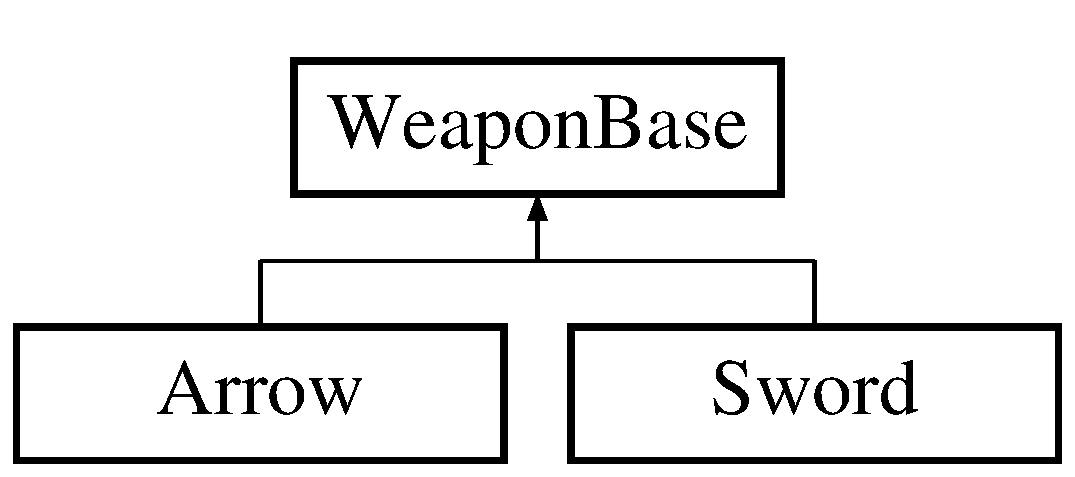
\includegraphics[height=2.000000cm]{class_weapon_base}
\end{center}
\end{figure}
\subsection*{公開メンバ関数}
\begin{DoxyCompactItemize}
\item 
virtual bool \mbox{\hyperlink{class_weapon_base_a1bab9c7fb9524db754bebbbcbf6c2fd9}{Attack}} (bool, const \mbox{\hyperlink{common_8h_ab1cb35b3a17c398d8ef71d5f779808bf}{Vec3}} \&)=0
\item 
virtual void \mbox{\hyperlink{class_weapon_base_a25cd4c351638b76377e93341a9545712}{Weapon\+Start}} ()=0
\item 
virtual void \mbox{\hyperlink{class_weapon_base_aa1e3d02353273ab72a71cc3a1563636a}{Weapon\+Update}} (const \mbox{\hyperlink{common_8h_ab1cb35b3a17c398d8ef71d5f779808bf}{Vec3}} \&, bool)=0
\item 
virtual void \mbox{\hyperlink{class_weapon_base_af308d16d3892c3ffaeedf74b08e761b9}{Weapon\+Render}} (const \mbox{\hyperlink{common_8h_a1c43cb8f0d8a41901f3ce4c67dbbce20}{Transform}} \&=\mbox{\hyperlink{common_8h_a1c43cb8f0d8a41901f3ce4c67dbbce20}{Transform}}\{ saki\+::vector3\+\_\+zero$<$ float $>$, saki\+::vector3\+\_\+zero$<$ float $>$, saki\+::vector3\+\_\+zero$<$ float $>$ \})=0
\item 
virtual void \mbox{\hyperlink{class_weapon_base_a417784a8c8bf73cd398a77b922fc110c}{Weapon\+Destroy}} ()=0
\item 
virtual \mbox{\hyperlink{class_weapon_base_a311bee6c8496581f21068867be48762f}{$\sim$\+Weapon\+Base}} ()
\end{DoxyCompactItemize}
\subsection*{公開変数類}
\begin{DoxyCompactItemize}
\item 
bool \mbox{\hyperlink{class_weapon_base_a54883e3ecbc54ff42ea381a17ef8cf8f}{weapon\+\_\+enabled}} = true
\end{DoxyCompactItemize}


\subsection{詳解}
武器のスーパークラス 

\subsection{構築子と解体子}
\mbox{\Hypertarget{class_weapon_base_a311bee6c8496581f21068867be48762f}\label{class_weapon_base_a311bee6c8496581f21068867be48762f}} 
\index{Weapon\+Base@{Weapon\+Base}!````~Weapon\+Base@{$\sim$\+Weapon\+Base}}
\index{````~Weapon\+Base@{$\sim$\+Weapon\+Base}!Weapon\+Base@{Weapon\+Base}}
\subsubsection{\texorpdfstring{$\sim$\+Weapon\+Base()}{~WeaponBase()}}
{\footnotesize\ttfamily virtual Weapon\+Base\+::$\sim$\+Weapon\+Base (\begin{DoxyParamCaption}{ }\end{DoxyParamCaption})\hspace{0.3cm}{\ttfamily [inline]}, {\ttfamily [virtual]}}



\subsection{関数詳解}
\mbox{\Hypertarget{class_weapon_base_a1bab9c7fb9524db754bebbbcbf6c2fd9}\label{class_weapon_base_a1bab9c7fb9524db754bebbbcbf6c2fd9}} 
\index{Weapon\+Base@{Weapon\+Base}!Attack@{Attack}}
\index{Attack@{Attack}!Weapon\+Base@{Weapon\+Base}}
\subsubsection{\texorpdfstring{Attack()}{Attack()}}
{\footnotesize\ttfamily virtual bool Weapon\+Base\+::\+Attack (\begin{DoxyParamCaption}\item[{bool}]{,  }\item[{const \mbox{\hyperlink{common_8h_ab1cb35b3a17c398d8ef71d5f779808bf}{Vec3}} \&}]{ }\end{DoxyParamCaption})\hspace{0.3cm}{\ttfamily [pure virtual]}}



\mbox{\hyperlink{class_sword_a6c8642e6a8f1d6152abce6c84bf6d21b}{Sword}}, \mbox{\hyperlink{class_arrow_a98ea469bf0b21635b2d2dadb69c72240}{Arrow}}で実装されています。

\mbox{\Hypertarget{class_weapon_base_a417784a8c8bf73cd398a77b922fc110c}\label{class_weapon_base_a417784a8c8bf73cd398a77b922fc110c}} 
\index{Weapon\+Base@{Weapon\+Base}!Weapon\+Destroy@{Weapon\+Destroy}}
\index{Weapon\+Destroy@{Weapon\+Destroy}!Weapon\+Base@{Weapon\+Base}}
\subsubsection{\texorpdfstring{Weapon\+Destroy()}{WeaponDestroy()}}
{\footnotesize\ttfamily virtual void Weapon\+Base\+::\+Weapon\+Destroy (\begin{DoxyParamCaption}{ }\end{DoxyParamCaption})\hspace{0.3cm}{\ttfamily [pure virtual]}}



\mbox{\hyperlink{class_sword_a3f60d8b24b7847d6a84f0941820b711d}{Sword}}, \mbox{\hyperlink{class_arrow_a1101d1159771b5c428afd3c7a6a0a4df}{Arrow}}で実装されています。

\mbox{\Hypertarget{class_weapon_base_af308d16d3892c3ffaeedf74b08e761b9}\label{class_weapon_base_af308d16d3892c3ffaeedf74b08e761b9}} 
\index{Weapon\+Base@{Weapon\+Base}!Weapon\+Render@{Weapon\+Render}}
\index{Weapon\+Render@{Weapon\+Render}!Weapon\+Base@{Weapon\+Base}}
\subsubsection{\texorpdfstring{Weapon\+Render()}{WeaponRender()}}
{\footnotesize\ttfamily virtual void Weapon\+Base\+::\+Weapon\+Render (\begin{DoxyParamCaption}\item[{const \mbox{\hyperlink{common_8h_a1c43cb8f0d8a41901f3ce4c67dbbce20}{Transform}} \&}]{ = {\ttfamily \mbox{\hyperlink{common_8h_a1c43cb8f0d8a41901f3ce4c67dbbce20}{Transform}}\{~saki\+:\+:vector3\+\_\+zero$<$~float~$>$,~saki\+:\+:vector3\+\_\+zero$<$~float~$>$,~saki\+:\+:vector3\+\_\+zero$<$~float~$>$~\}} }\end{DoxyParamCaption})\hspace{0.3cm}{\ttfamily [pure virtual]}}



\mbox{\hyperlink{class_sword_ac80e3b54ef5572eae1e4760d14383f4f}{Sword}}, \mbox{\hyperlink{class_arrow_af9e54760156a77a15ad98a88f712ebdb}{Arrow}}で実装されています。

\mbox{\Hypertarget{class_weapon_base_a25cd4c351638b76377e93341a9545712}\label{class_weapon_base_a25cd4c351638b76377e93341a9545712}} 
\index{Weapon\+Base@{Weapon\+Base}!Weapon\+Start@{Weapon\+Start}}
\index{Weapon\+Start@{Weapon\+Start}!Weapon\+Base@{Weapon\+Base}}
\subsubsection{\texorpdfstring{Weapon\+Start()}{WeaponStart()}}
{\footnotesize\ttfamily virtual void Weapon\+Base\+::\+Weapon\+Start (\begin{DoxyParamCaption}{ }\end{DoxyParamCaption})\hspace{0.3cm}{\ttfamily [pure virtual]}}



\mbox{\hyperlink{class_sword_af9027f627d1db6c0ac21d2aa842cff69}{Sword}}, \mbox{\hyperlink{class_arrow_a085b5bd5f9e3ce25a081b502f9989f33}{Arrow}}で実装されています。

\mbox{\Hypertarget{class_weapon_base_aa1e3d02353273ab72a71cc3a1563636a}\label{class_weapon_base_aa1e3d02353273ab72a71cc3a1563636a}} 
\index{Weapon\+Base@{Weapon\+Base}!Weapon\+Update@{Weapon\+Update}}
\index{Weapon\+Update@{Weapon\+Update}!Weapon\+Base@{Weapon\+Base}}
\subsubsection{\texorpdfstring{Weapon\+Update()}{WeaponUpdate()}}
{\footnotesize\ttfamily virtual void Weapon\+Base\+::\+Weapon\+Update (\begin{DoxyParamCaption}\item[{const \mbox{\hyperlink{common_8h_ab1cb35b3a17c398d8ef71d5f779808bf}{Vec3}} \&}]{,  }\item[{bool}]{ }\end{DoxyParamCaption})\hspace{0.3cm}{\ttfamily [pure virtual]}}



\mbox{\hyperlink{class_sword_a5fda2f72829b6256ffc3fb18d9d065e8}{Sword}}, \mbox{\hyperlink{class_arrow_afb6110035cba7b850d12755570163b29}{Arrow}}で実装されています。



\subsection{メンバ詳解}
\mbox{\Hypertarget{class_weapon_base_a54883e3ecbc54ff42ea381a17ef8cf8f}\label{class_weapon_base_a54883e3ecbc54ff42ea381a17ef8cf8f}} 
\index{Weapon\+Base@{Weapon\+Base}!weapon\+\_\+enabled@{weapon\+\_\+enabled}}
\index{weapon\+\_\+enabled@{weapon\+\_\+enabled}!Weapon\+Base@{Weapon\+Base}}
\subsubsection{\texorpdfstring{weapon\+\_\+enabled}{weapon\_enabled}}
{\footnotesize\ttfamily bool Weapon\+Base\+::weapon\+\_\+enabled = true}



このクラス詳解は次のファイルから抽出されました\+:\begin{DoxyCompactItemize}
\item 
C\+:/\+Users/tokir/\+Documents/\+Git\+Hub/\+Weapon\+Merchant\+Adventure/src/src/object/weapon/base/\mbox{\hyperlink{weapon__base_8h}{weapon\+\_\+base.\+h}}\end{DoxyCompactItemize}

\chapter{ファイル詳解}
\hypertarget{accumulate_8h}{}\section{C\+:/\+Users/tokir/\+Documents/\+Git\+Hub/\+Weapon\+Merchant\+Adventure/src/lib/saki/accumulate/accumulate.h ファイル}
\label{accumulate_8h}\index{C\+:/\+Users/tokir/\+Documents/\+Git\+Hub/\+Weapon\+Merchant\+Adventure/src/lib/saki/accumulate/accumulate.\+h@{C\+:/\+Users/tokir/\+Documents/\+Git\+Hub/\+Weapon\+Merchant\+Adventure/src/lib/saki/accumulate/accumulate.\+h}}


既存のaccumulate関数の簡略化  


{\ttfamily \#include $<$type\+\_\+traits$>$}\newline
\subsection*{名前空間}
\begin{DoxyCompactItemize}
\item 
 \mbox{\hyperlink{namespacesaki}{saki}}
\end{DoxyCompactItemize}
\subsection*{マクロ定義}
\begin{DoxyCompactItemize}
\item 
\#define \mbox{\hyperlink{accumulate_8h_a929b0b8e319f7448b342dd1337cf62de}{S\+A\+K\+I\+\_\+\+A\+C\+C\+U\+M\+U\+L\+A\+T\+E\+\_\+2018\+\_\+12\+\_\+06}}
\end{DoxyCompactItemize}
\subsection*{関数}
\begin{DoxyCompactItemize}
\item 
{\footnotesize template$<$typename Container $>$ }\\auto \mbox{\hyperlink{namespacesaki_a981cc67b0d421b1836678c3ac4069afd}{saki\+::accumulate}} (Container \&\&con, typename std\+::remove\+\_\+reference\+\_\+t$<$ Container $>$\+::value\+\_\+type init=0)
\begin{DoxyCompactList}\small\item\em 全ての値の合計 \end{DoxyCompactList}\item 
{\footnotesize template$<$typename Container , typename Binary\+Operation $>$ }\\auto \mbox{\hyperlink{namespacesaki_acb8c3f650d3b5d3b06259b91bd7ad85d}{saki\+::accumulate}} (Container \&\&con, Binary\+Operation \&\&binary\+\_\+op, typename std\+::remove\+\_\+reference\+\_\+t$<$ Container $>$\+::value\+\_\+type init=0)
\begin{DoxyCompactList}\small\item\em 引数が2つの関数を指定し、それをすべての要素で回す \end{DoxyCompactList}\end{DoxyCompactItemize}


\subsection{詳解}
既存のaccumulate関数の簡略化 

\begin{DoxyAuthor}{著者}
石山 悠 
\end{DoxyAuthor}
\begin{DoxyDate}{日付}
2018/12/06 
\end{DoxyDate}


\subsection{マクロ定義詳解}
\mbox{\Hypertarget{accumulate_8h_a929b0b8e319f7448b342dd1337cf62de}\label{accumulate_8h_a929b0b8e319f7448b342dd1337cf62de}} 
\index{accumulate.\+h@{accumulate.\+h}!S\+A\+K\+I\+\_\+\+A\+C\+C\+U\+M\+U\+L\+A\+T\+E\+\_\+2018\+\_\+12\+\_\+06@{S\+A\+K\+I\+\_\+\+A\+C\+C\+U\+M\+U\+L\+A\+T\+E\+\_\+2018\+\_\+12\+\_\+06}}
\index{S\+A\+K\+I\+\_\+\+A\+C\+C\+U\+M\+U\+L\+A\+T\+E\+\_\+2018\+\_\+12\+\_\+06@{S\+A\+K\+I\+\_\+\+A\+C\+C\+U\+M\+U\+L\+A\+T\+E\+\_\+2018\+\_\+12\+\_\+06}!accumulate.\+h@{accumulate.\+h}}
\subsubsection{\texorpdfstring{S\+A\+K\+I\+\_\+\+A\+C\+C\+U\+M\+U\+L\+A\+T\+E\+\_\+2018\+\_\+12\+\_\+06}{SAKI\_ACCUMULATE\_2018\_12\_06}}
{\footnotesize\ttfamily \#define S\+A\+K\+I\+\_\+\+A\+C\+C\+U\+M\+U\+L\+A\+T\+E\+\_\+2018\+\_\+12\+\_\+06}


\hypertarget{angle__math_8h}{}\section{C\+:/\+Users/tokir/\+Documents/\+Git\+Hub/\+Weapon\+Merchant\+Adventure/src/lib/saki/angle\+\_\+math/angle\+\_\+math.h ファイル}
\label{angle__math_8h}\index{C\+:/\+Users/tokir/\+Documents/\+Git\+Hub/\+Weapon\+Merchant\+Adventure/src/lib/saki/angle\+\_\+math/angle\+\_\+math.\+h@{C\+:/\+Users/tokir/\+Documents/\+Git\+Hub/\+Weapon\+Merchant\+Adventure/src/lib/saki/angle\+\_\+math/angle\+\_\+math.\+h}}


簡易インクルード(angle\+\_\+math)  


{\ttfamily \#include $<$saki/angle\+\_\+math/degree\+\_\+radian\+\_\+conversion.\+h$>$}\newline
\subsection*{マクロ定義}
\begin{DoxyCompactItemize}
\item 
\#define \mbox{\hyperlink{angle__math_8h_a1498ecba91dfd566d2231b5fa63c76d0}{S\+A\+K\+I\+\_\+\+A\+N\+G\+L\+E\+\_\+\+M\+A\+T\+H\+\_\+2018\+\_\+11\+\_\+22}}
\end{DoxyCompactItemize}


\subsection{詳解}
簡易インクルード(angle\+\_\+math) 

簡易インクルード(binary\+\_\+operator)

\begin{DoxyAuthor}{著者}
石山 悠 
\end{DoxyAuthor}
\begin{DoxyDate}{日付}
2018/11/22
\end{DoxyDate}
\begin{DoxyAuthor}{著者}
石山 悠 
\end{DoxyAuthor}
\begin{DoxyDate}{日付}
2018/12/08 
\end{DoxyDate}


\subsection{マクロ定義詳解}
\mbox{\Hypertarget{angle__math_8h_a1498ecba91dfd566d2231b5fa63c76d0}\label{angle__math_8h_a1498ecba91dfd566d2231b5fa63c76d0}} 
\index{angle\+\_\+math.\+h@{angle\+\_\+math.\+h}!S\+A\+K\+I\+\_\+\+A\+N\+G\+L\+E\+\_\+\+M\+A\+T\+H\+\_\+2018\+\_\+11\+\_\+22@{S\+A\+K\+I\+\_\+\+A\+N\+G\+L\+E\+\_\+\+M\+A\+T\+H\+\_\+2018\+\_\+11\+\_\+22}}
\index{S\+A\+K\+I\+\_\+\+A\+N\+G\+L\+E\+\_\+\+M\+A\+T\+H\+\_\+2018\+\_\+11\+\_\+22@{S\+A\+K\+I\+\_\+\+A\+N\+G\+L\+E\+\_\+\+M\+A\+T\+H\+\_\+2018\+\_\+11\+\_\+22}!angle\+\_\+math.\+h@{angle\+\_\+math.\+h}}
\subsubsection{\texorpdfstring{S\+A\+K\+I\+\_\+\+A\+N\+G\+L\+E\+\_\+\+M\+A\+T\+H\+\_\+2018\+\_\+11\+\_\+22}{SAKI\_ANGLE\_MATH\_2018\_11\_22}}
{\footnotesize\ttfamily \#define S\+A\+K\+I\+\_\+\+A\+N\+G\+L\+E\+\_\+\+M\+A\+T\+H\+\_\+2018\+\_\+11\+\_\+22}


\hypertarget{degree__radian__conversion_8h}{}\section{C\+:/\+Users/tokir/\+Documents/\+Git\+Hub/\+Weapon\+Merchant\+Adventure/src/lib/saki/angle\+\_\+math/degree\+\_\+radian\+\_\+conversion.h ファイル}
\label{degree__radian__conversion_8h}\index{C\+:/\+Users/tokir/\+Documents/\+Git\+Hub/\+Weapon\+Merchant\+Adventure/src/lib/saki/angle\+\_\+math/degree\+\_\+radian\+\_\+conversion.\+h@{C\+:/\+Users/tokir/\+Documents/\+Git\+Hub/\+Weapon\+Merchant\+Adventure/src/lib/saki/angle\+\_\+math/degree\+\_\+radian\+\_\+conversion.\+h}}


Degreeから\+Radian、\+Radianから\+Degreeへの変換  


{\ttfamily \#include $<$saki/pi.\+h$>$}\newline
\subsection*{名前空間}
\begin{DoxyCompactItemize}
\item 
 \mbox{\hyperlink{namespacesaki}{saki}}
\end{DoxyCompactItemize}
\subsection*{マクロ定義}
\begin{DoxyCompactItemize}
\item 
\#define \mbox{\hyperlink{degree__radian__conversion_8h_a9884d65768d5e43d3d1db831c2079bbb}{S\+A\+K\+I\+\_\+\+D\+E\+G\+R\+E\+E\+\_\+\+R\+A\+D\+I\+A\+N\+\_\+\+C\+O\+N\+V\+E\+R\+S\+I\+O\+N\+\_\+2018\+\_\+11\+\_\+13}}
\end{DoxyCompactItemize}
\subsection*{関数}
\begin{DoxyCompactItemize}
\item 
{\footnotesize template$<$typename Rad  = double, typename Deg $>$ }\\constexpr Rad \mbox{\hyperlink{namespacesaki_aae246ec576e9e2da23c0c142e6fc4d6a}{saki\+::to\+\_\+radian}} (Deg deg)
\begin{DoxyCompactList}\small\item\em Degreeから\+Radianに変換 \end{DoxyCompactList}\item 
{\footnotesize template$<$typename Deg  = double, typename Rad $>$ }\\constexpr Deg \mbox{\hyperlink{namespacesaki_aa28ebe642bd2c0e608e2a61c34b3d7a5}{saki\+::to\+\_\+degree}} (Rad rad)
\begin{DoxyCompactList}\small\item\em Radianから\+Degreeに変換 \end{DoxyCompactList}\end{DoxyCompactItemize}


\subsection{詳解}
Degreeから\+Radian、\+Radianから\+Degreeへの変換 

\begin{DoxyAuthor}{著者}
石山 悠 
\end{DoxyAuthor}
\begin{DoxyDate}{日付}
2018/11/13 
\end{DoxyDate}


\subsection{マクロ定義詳解}
\mbox{\Hypertarget{degree__radian__conversion_8h_a9884d65768d5e43d3d1db831c2079bbb}\label{degree__radian__conversion_8h_a9884d65768d5e43d3d1db831c2079bbb}} 
\index{degree\+\_\+radian\+\_\+conversion.\+h@{degree\+\_\+radian\+\_\+conversion.\+h}!S\+A\+K\+I\+\_\+\+D\+E\+G\+R\+E\+E\+\_\+\+R\+A\+D\+I\+A\+N\+\_\+\+C\+O\+N\+V\+E\+R\+S\+I\+O\+N\+\_\+2018\+\_\+11\+\_\+13@{S\+A\+K\+I\+\_\+\+D\+E\+G\+R\+E\+E\+\_\+\+R\+A\+D\+I\+A\+N\+\_\+\+C\+O\+N\+V\+E\+R\+S\+I\+O\+N\+\_\+2018\+\_\+11\+\_\+13}}
\index{S\+A\+K\+I\+\_\+\+D\+E\+G\+R\+E\+E\+\_\+\+R\+A\+D\+I\+A\+N\+\_\+\+C\+O\+N\+V\+E\+R\+S\+I\+O\+N\+\_\+2018\+\_\+11\+\_\+13@{S\+A\+K\+I\+\_\+\+D\+E\+G\+R\+E\+E\+\_\+\+R\+A\+D\+I\+A\+N\+\_\+\+C\+O\+N\+V\+E\+R\+S\+I\+O\+N\+\_\+2018\+\_\+11\+\_\+13}!degree\+\_\+radian\+\_\+conversion.\+h@{degree\+\_\+radian\+\_\+conversion.\+h}}
\subsubsection{\texorpdfstring{S\+A\+K\+I\+\_\+\+D\+E\+G\+R\+E\+E\+\_\+\+R\+A\+D\+I\+A\+N\+\_\+\+C\+O\+N\+V\+E\+R\+S\+I\+O\+N\+\_\+2018\+\_\+11\+\_\+13}{SAKI\_DEGREE\_RADIAN\_CONVERSION\_2018\_11\_13}}
{\footnotesize\ttfamily \#define S\+A\+K\+I\+\_\+\+D\+E\+G\+R\+E\+E\+\_\+\+R\+A\+D\+I\+A\+N\+\_\+\+C\+O\+N\+V\+E\+R\+S\+I\+O\+N\+\_\+2018\+\_\+11\+\_\+13}


\hypertarget{addition_8h}{}\section{C\+:/\+Users/tokir/\+Documents/\+Git\+Hub/\+Weapon\+Merchant\+Adventure/src/lib/saki/binary\+\_\+operator/addition.h ファイル}
\label{addition_8h}\index{C\+:/\+Users/tokir/\+Documents/\+Git\+Hub/\+Weapon\+Merchant\+Adventure/src/lib/saki/binary\+\_\+operator/addition.\+h@{C\+:/\+Users/tokir/\+Documents/\+Git\+Hub/\+Weapon\+Merchant\+Adventure/src/lib/saki/binary\+\_\+operator/addition.\+h}}


足し算のオペレーターを呼び出すconstexpr関数オブジェクト  


\subsection*{クラス}
\begin{DoxyCompactItemize}
\item 
struct \mbox{\hyperlink{structsaki_1_1addition}{saki\+::addition}}
\begin{DoxyCompactList}\small\item\em 足し算のconstexpr対応した関数オブジェクト \end{DoxyCompactList}\end{DoxyCompactItemize}
\subsection*{名前空間}
\begin{DoxyCompactItemize}
\item 
 \mbox{\hyperlink{namespacesaki}{saki}}
\end{DoxyCompactItemize}
\subsection*{マクロ定義}
\begin{DoxyCompactItemize}
\item 
\#define \mbox{\hyperlink{addition_8h_a1b23bb9597189375bc9dafc02d09bf4e}{S\+A\+K\+I\+\_\+\+A\+D\+D\+I\+T\+I\+O\+N\+\_\+2018\+\_\+12\+\_\+08}}
\end{DoxyCompactItemize}


\subsection{詳解}
足し算のオペレーターを呼び出すconstexpr関数オブジェクト 

\begin{DoxyAuthor}{著者}
石山 悠 
\end{DoxyAuthor}
\begin{DoxyDate}{日付}
2018/12/08 
\end{DoxyDate}


\subsection{マクロ定義詳解}
\mbox{\Hypertarget{addition_8h_a1b23bb9597189375bc9dafc02d09bf4e}\label{addition_8h_a1b23bb9597189375bc9dafc02d09bf4e}} 
\index{addition.\+h@{addition.\+h}!S\+A\+K\+I\+\_\+\+A\+D\+D\+I\+T\+I\+O\+N\+\_\+2018\+\_\+12\+\_\+08@{S\+A\+K\+I\+\_\+\+A\+D\+D\+I\+T\+I\+O\+N\+\_\+2018\+\_\+12\+\_\+08}}
\index{S\+A\+K\+I\+\_\+\+A\+D\+D\+I\+T\+I\+O\+N\+\_\+2018\+\_\+12\+\_\+08@{S\+A\+K\+I\+\_\+\+A\+D\+D\+I\+T\+I\+O\+N\+\_\+2018\+\_\+12\+\_\+08}!addition.\+h@{addition.\+h}}
\subsubsection{\texorpdfstring{S\+A\+K\+I\+\_\+\+A\+D\+D\+I\+T\+I\+O\+N\+\_\+2018\+\_\+12\+\_\+08}{SAKI\_ADDITION\_2018\_12\_08}}
{\footnotesize\ttfamily \#define S\+A\+K\+I\+\_\+\+A\+D\+D\+I\+T\+I\+O\+N\+\_\+2018\+\_\+12\+\_\+08}


\hypertarget{binary__operator_8h}{}\section{C\+:/\+Users/tokir/\+Documents/\+Git\+Hub/\+Weapon\+Merchant\+Adventure/src/lib/saki/binary\+\_\+operator/binary\+\_\+operator.h ファイル}
\label{binary__operator_8h}\index{C\+:/\+Users/tokir/\+Documents/\+Git\+Hub/\+Weapon\+Merchant\+Adventure/src/lib/saki/binary\+\_\+operator/binary\+\_\+operator.\+h@{C\+:/\+Users/tokir/\+Documents/\+Git\+Hub/\+Weapon\+Merchant\+Adventure/src/lib/saki/binary\+\_\+operator/binary\+\_\+operator.\+h}}
{\ttfamily \#include $<$saki/binary\+\_\+operator/addition.\+h$>$}\newline
{\ttfamily \#include $<$saki/binary\+\_\+operator/division.\+h$>$}\newline
{\ttfamily \#include $<$saki/binary\+\_\+operator/multiplication.\+h$>$}\newline
{\ttfamily \#include $<$saki/binary\+\_\+operator/return\+\_\+param.\+h$>$}\newline
{\ttfamily \#include $<$saki/binary\+\_\+operator/subtraction.\+h$>$}\newline
\subsection*{マクロ定義}
\begin{DoxyCompactItemize}
\item 
\#define \mbox{\hyperlink{binary__operator_8h_a7256b1cdd2f524495661b957a63ea28c}{S\+A\+K\+I\+\_\+\+B\+I\+N\+A\+R\+Y\+\_\+\+O\+P\+E\+R\+A\+T\+O\+R\+\_\+2018\+\_\+11\+\_\+08}}
\end{DoxyCompactItemize}


\subsection{マクロ定義詳解}
\mbox{\Hypertarget{binary__operator_8h_a7256b1cdd2f524495661b957a63ea28c}\label{binary__operator_8h_a7256b1cdd2f524495661b957a63ea28c}} 
\index{binary\+\_\+operator.\+h@{binary\+\_\+operator.\+h}!S\+A\+K\+I\+\_\+\+B\+I\+N\+A\+R\+Y\+\_\+\+O\+P\+E\+R\+A\+T\+O\+R\+\_\+2018\+\_\+11\+\_\+08@{S\+A\+K\+I\+\_\+\+B\+I\+N\+A\+R\+Y\+\_\+\+O\+P\+E\+R\+A\+T\+O\+R\+\_\+2018\+\_\+11\+\_\+08}}
\index{S\+A\+K\+I\+\_\+\+B\+I\+N\+A\+R\+Y\+\_\+\+O\+P\+E\+R\+A\+T\+O\+R\+\_\+2018\+\_\+11\+\_\+08@{S\+A\+K\+I\+\_\+\+B\+I\+N\+A\+R\+Y\+\_\+\+O\+P\+E\+R\+A\+T\+O\+R\+\_\+2018\+\_\+11\+\_\+08}!binary\+\_\+operator.\+h@{binary\+\_\+operator.\+h}}
\subsubsection{\texorpdfstring{S\+A\+K\+I\+\_\+\+B\+I\+N\+A\+R\+Y\+\_\+\+O\+P\+E\+R\+A\+T\+O\+R\+\_\+2018\+\_\+11\+\_\+08}{SAKI\_BINARY\_OPERATOR\_2018\_11\_08}}
{\footnotesize\ttfamily \#define S\+A\+K\+I\+\_\+\+B\+I\+N\+A\+R\+Y\+\_\+\+O\+P\+E\+R\+A\+T\+O\+R\+\_\+2018\+\_\+11\+\_\+08}


\hypertarget{division_8h}{}\section{C\+:/\+Users/tokir/\+Documents/\+Git\+Hub/\+Weapon\+Merchant\+Adventure/src/lib/saki/binary\+\_\+operator/division.h ファイル}
\label{division_8h}\index{C\+:/\+Users/tokir/\+Documents/\+Git\+Hub/\+Weapon\+Merchant\+Adventure/src/lib/saki/binary\+\_\+operator/division.\+h@{C\+:/\+Users/tokir/\+Documents/\+Git\+Hub/\+Weapon\+Merchant\+Adventure/src/lib/saki/binary\+\_\+operator/division.\+h}}


割り算のオペレーターを呼び出すconstexpr関数オブジェクト  


\subsection*{クラス}
\begin{DoxyCompactItemize}
\item 
struct \mbox{\hyperlink{structsaki_1_1division}{saki\+::division}}
\begin{DoxyCompactList}\small\item\em 割り算のconstexpr対応した関数オブジェクト \end{DoxyCompactList}\end{DoxyCompactItemize}
\subsection*{名前空間}
\begin{DoxyCompactItemize}
\item 
 \mbox{\hyperlink{namespacesaki}{saki}}
\end{DoxyCompactItemize}
\subsection*{マクロ定義}
\begin{DoxyCompactItemize}
\item 
\#define \mbox{\hyperlink{division_8h_af127b2c9efa823d1128a02b307e93b48}{S\+A\+K\+I\+\_\+\+D\+I\+V\+I\+S\+I\+O\+N\+\_\+2018\+\_\+12\+\_\+08}}
\end{DoxyCompactItemize}


\subsection{詳解}
割り算のオペレーターを呼び出すconstexpr関数オブジェクト 

\begin{DoxyAuthor}{著者}
石山 悠 
\end{DoxyAuthor}
\begin{DoxyDate}{日付}
2018/12/08 
\end{DoxyDate}


\subsection{マクロ定義詳解}
\mbox{\Hypertarget{division_8h_af127b2c9efa823d1128a02b307e93b48}\label{division_8h_af127b2c9efa823d1128a02b307e93b48}} 
\index{division.\+h@{division.\+h}!S\+A\+K\+I\+\_\+\+D\+I\+V\+I\+S\+I\+O\+N\+\_\+2018\+\_\+12\+\_\+08@{S\+A\+K\+I\+\_\+\+D\+I\+V\+I\+S\+I\+O\+N\+\_\+2018\+\_\+12\+\_\+08}}
\index{S\+A\+K\+I\+\_\+\+D\+I\+V\+I\+S\+I\+O\+N\+\_\+2018\+\_\+12\+\_\+08@{S\+A\+K\+I\+\_\+\+D\+I\+V\+I\+S\+I\+O\+N\+\_\+2018\+\_\+12\+\_\+08}!division.\+h@{division.\+h}}
\subsubsection{\texorpdfstring{S\+A\+K\+I\+\_\+\+D\+I\+V\+I\+S\+I\+O\+N\+\_\+2018\+\_\+12\+\_\+08}{SAKI\_DIVISION\_2018\_12\_08}}
{\footnotesize\ttfamily \#define S\+A\+K\+I\+\_\+\+D\+I\+V\+I\+S\+I\+O\+N\+\_\+2018\+\_\+12\+\_\+08}


\hypertarget{multiplication_8h}{}\section{C\+:/\+Users/tokir/\+Documents/\+Git\+Hub/\+Weapon\+Merchant\+Adventure/src/lib/saki/binary\+\_\+operator/multiplication.h ファイル}
\label{multiplication_8h}\index{C\+:/\+Users/tokir/\+Documents/\+Git\+Hub/\+Weapon\+Merchant\+Adventure/src/lib/saki/binary\+\_\+operator/multiplication.\+h@{C\+:/\+Users/tokir/\+Documents/\+Git\+Hub/\+Weapon\+Merchant\+Adventure/src/lib/saki/binary\+\_\+operator/multiplication.\+h}}


掛け算のオペレーターを呼び出すconstexpr関数オブジェクト  


\subsection*{クラス}
\begin{DoxyCompactItemize}
\item 
struct \mbox{\hyperlink{structsaki_1_1multiplication}{saki\+::multiplication}}
\begin{DoxyCompactList}\small\item\em 掛け算のconstexpr対応した関数オブジェクト \end{DoxyCompactList}\end{DoxyCompactItemize}
\subsection*{名前空間}
\begin{DoxyCompactItemize}
\item 
 \mbox{\hyperlink{namespacesaki}{saki}}
\end{DoxyCompactItemize}
\subsection*{マクロ定義}
\begin{DoxyCompactItemize}
\item 
\#define \mbox{\hyperlink{multiplication_8h_a3db10324c3cb4ea343b4fe3e22a91c91}{S\+A\+K\+I\+\_\+\+M\+U\+L\+T\+I\+P\+L\+I\+C\+A\+T\+I\+O\+N\+\_\+2018\+\_\+12\+\_\+08}}
\end{DoxyCompactItemize}


\subsection{詳解}
掛け算のオペレーターを呼び出すconstexpr関数オブジェクト 

\begin{DoxyAuthor}{著者}
石山 悠 
\end{DoxyAuthor}
\begin{DoxyDate}{日付}
2018/12/08 
\end{DoxyDate}


\subsection{マクロ定義詳解}
\mbox{\Hypertarget{multiplication_8h_a3db10324c3cb4ea343b4fe3e22a91c91}\label{multiplication_8h_a3db10324c3cb4ea343b4fe3e22a91c91}} 
\index{multiplication.\+h@{multiplication.\+h}!S\+A\+K\+I\+\_\+\+M\+U\+L\+T\+I\+P\+L\+I\+C\+A\+T\+I\+O\+N\+\_\+2018\+\_\+12\+\_\+08@{S\+A\+K\+I\+\_\+\+M\+U\+L\+T\+I\+P\+L\+I\+C\+A\+T\+I\+O\+N\+\_\+2018\+\_\+12\+\_\+08}}
\index{S\+A\+K\+I\+\_\+\+M\+U\+L\+T\+I\+P\+L\+I\+C\+A\+T\+I\+O\+N\+\_\+2018\+\_\+12\+\_\+08@{S\+A\+K\+I\+\_\+\+M\+U\+L\+T\+I\+P\+L\+I\+C\+A\+T\+I\+O\+N\+\_\+2018\+\_\+12\+\_\+08}!multiplication.\+h@{multiplication.\+h}}
\subsubsection{\texorpdfstring{S\+A\+K\+I\+\_\+\+M\+U\+L\+T\+I\+P\+L\+I\+C\+A\+T\+I\+O\+N\+\_\+2018\+\_\+12\+\_\+08}{SAKI\_MULTIPLICATION\_2018\_12\_08}}
{\footnotesize\ttfamily \#define S\+A\+K\+I\+\_\+\+M\+U\+L\+T\+I\+P\+L\+I\+C\+A\+T\+I\+O\+N\+\_\+2018\+\_\+12\+\_\+08}


\hypertarget{return__param_8h}{}\section{C\+:/\+Users/tokir/\+Documents/\+Git\+Hub/\+Weapon\+Merchant\+Adventure/src/lib/saki/binary\+\_\+operator/return\+\_\+param.h ファイル}
\label{return__param_8h}\index{C\+:/\+Users/tokir/\+Documents/\+Git\+Hub/\+Weapon\+Merchant\+Adventure/src/lib/saki/binary\+\_\+operator/return\+\_\+param.\+h@{C\+:/\+Users/tokir/\+Documents/\+Git\+Hub/\+Weapon\+Merchant\+Adventure/src/lib/saki/binary\+\_\+operator/return\+\_\+param.\+h}}


そのまま引数の値を返す  


\subsection*{クラス}
\begin{DoxyCompactItemize}
\item 
struct \mbox{\hyperlink{structsaki_1_1_return_param}{saki\+::\+Return\+Param}}
\begin{DoxyCompactList}\small\item\em そのまま引数を返す関数オブジェクト \end{DoxyCompactList}\end{DoxyCompactItemize}
\subsection*{名前空間}
\begin{DoxyCompactItemize}
\item 
 \mbox{\hyperlink{namespacesaki}{saki}}
\end{DoxyCompactItemize}
\subsection*{マクロ定義}
\begin{DoxyCompactItemize}
\item 
\#define \mbox{\hyperlink{return__param_8h_a4e8c368db3b4137452bfa1f80a931fea}{S\+A\+K\+I\+\_\+\+R\+E\+T\+U\+R\+N\+\_\+\+P\+A\+R\+A\+M\+\_\+2018\+\_\+12\+\_\+10}}
\end{DoxyCompactItemize}


\subsection{詳解}
そのまま引数の値を返す 

\begin{DoxyAuthor}{著者}
石山 悠 
\end{DoxyAuthor}
\begin{DoxyDate}{日付}
2018/12/10 
\end{DoxyDate}


\subsection{マクロ定義詳解}
\mbox{\Hypertarget{return__param_8h_a4e8c368db3b4137452bfa1f80a931fea}\label{return__param_8h_a4e8c368db3b4137452bfa1f80a931fea}} 
\index{return\+\_\+param.\+h@{return\+\_\+param.\+h}!S\+A\+K\+I\+\_\+\+R\+E\+T\+U\+R\+N\+\_\+\+P\+A\+R\+A\+M\+\_\+2018\+\_\+12\+\_\+10@{S\+A\+K\+I\+\_\+\+R\+E\+T\+U\+R\+N\+\_\+\+P\+A\+R\+A\+M\+\_\+2018\+\_\+12\+\_\+10}}
\index{S\+A\+K\+I\+\_\+\+R\+E\+T\+U\+R\+N\+\_\+\+P\+A\+R\+A\+M\+\_\+2018\+\_\+12\+\_\+10@{S\+A\+K\+I\+\_\+\+R\+E\+T\+U\+R\+N\+\_\+\+P\+A\+R\+A\+M\+\_\+2018\+\_\+12\+\_\+10}!return\+\_\+param.\+h@{return\+\_\+param.\+h}}
\subsubsection{\texorpdfstring{S\+A\+K\+I\+\_\+\+R\+E\+T\+U\+R\+N\+\_\+\+P\+A\+R\+A\+M\+\_\+2018\+\_\+12\+\_\+10}{SAKI\_RETURN\_PARAM\_2018\_12\_10}}
{\footnotesize\ttfamily \#define S\+A\+K\+I\+\_\+\+R\+E\+T\+U\+R\+N\+\_\+\+P\+A\+R\+A\+M\+\_\+2018\+\_\+12\+\_\+10}


\hypertarget{subtraction_8h}{}\section{C\+:/\+Users/tokir/\+Documents/\+Git\+Hub/\+Weapon\+Merchant\+Adventure/src/lib/saki/binary\+\_\+operator/subtraction.h ファイル}
\label{subtraction_8h}\index{C\+:/\+Users/tokir/\+Documents/\+Git\+Hub/\+Weapon\+Merchant\+Adventure/src/lib/saki/binary\+\_\+operator/subtraction.\+h@{C\+:/\+Users/tokir/\+Documents/\+Git\+Hub/\+Weapon\+Merchant\+Adventure/src/lib/saki/binary\+\_\+operator/subtraction.\+h}}


引き算のオペレーターを呼び出すconstexpr関数オブジェクト  


\subsection*{クラス}
\begin{DoxyCompactItemize}
\item 
struct \mbox{\hyperlink{structsaki_1_1subtraction}{saki\+::subtraction}}
\begin{DoxyCompactList}\small\item\em 引き算のconstexpr対応した関数オブジェクト \end{DoxyCompactList}\end{DoxyCompactItemize}
\subsection*{名前空間}
\begin{DoxyCompactItemize}
\item 
 \mbox{\hyperlink{namespacesaki}{saki}}
\end{DoxyCompactItemize}
\subsection*{マクロ定義}
\begin{DoxyCompactItemize}
\item 
\#define \mbox{\hyperlink{subtraction_8h_acf3307ef195db739d019e6281a2ec57f}{S\+A\+K\+I\+\_\+\+S\+U\+B\+T\+R\+A\+C\+T\+I\+O\+N\+\_\+2018\+\_\+12\+\_\+08}}
\end{DoxyCompactItemize}


\subsection{詳解}
引き算のオペレーターを呼び出すconstexpr関数オブジェクト 

\begin{DoxyAuthor}{著者}
石山 悠 
\end{DoxyAuthor}
\begin{DoxyDate}{日付}
2018/12/08 
\end{DoxyDate}


\subsection{マクロ定義詳解}
\mbox{\Hypertarget{subtraction_8h_acf3307ef195db739d019e6281a2ec57f}\label{subtraction_8h_acf3307ef195db739d019e6281a2ec57f}} 
\index{subtraction.\+h@{subtraction.\+h}!S\+A\+K\+I\+\_\+\+S\+U\+B\+T\+R\+A\+C\+T\+I\+O\+N\+\_\+2018\+\_\+12\+\_\+08@{S\+A\+K\+I\+\_\+\+S\+U\+B\+T\+R\+A\+C\+T\+I\+O\+N\+\_\+2018\+\_\+12\+\_\+08}}
\index{S\+A\+K\+I\+\_\+\+S\+U\+B\+T\+R\+A\+C\+T\+I\+O\+N\+\_\+2018\+\_\+12\+\_\+08@{S\+A\+K\+I\+\_\+\+S\+U\+B\+T\+R\+A\+C\+T\+I\+O\+N\+\_\+2018\+\_\+12\+\_\+08}!subtraction.\+h@{subtraction.\+h}}
\subsubsection{\texorpdfstring{S\+A\+K\+I\+\_\+\+S\+U\+B\+T\+R\+A\+C\+T\+I\+O\+N\+\_\+2018\+\_\+12\+\_\+08}{SAKI\_SUBTRACTION\_2018\_12\_08}}
{\footnotesize\ttfamily \#define S\+A\+K\+I\+\_\+\+S\+U\+B\+T\+R\+A\+C\+T\+I\+O\+N\+\_\+2018\+\_\+12\+\_\+08}


\hypertarget{clock_8h}{}\section{C\+:/\+Users/tokir/\+Documents/\+Git\+Hub/\+Weapon\+Merchant\+Adventure/src/lib/saki/clock/clock.h ファイル}
\label{clock_8h}\index{C\+:/\+Users/tokir/\+Documents/\+Git\+Hub/\+Weapon\+Merchant\+Adventure/src/lib/saki/clock/clock.\+h@{C\+:/\+Users/tokir/\+Documents/\+Git\+Hub/\+Weapon\+Merchant\+Adventure/src/lib/saki/clock/clock.\+h}}


時間を測るクラス  


{\ttfamily \#include $<$saki/singleton/singleton.\+h$>$}\newline
{\ttfamily \#include $<$ctime$>$}\newline
\subsection*{クラス}
\begin{DoxyCompactItemize}
\item 
class \mbox{\hyperlink{classsaki_1_1_clock}{saki\+::\+Clock}}
\begin{DoxyCompactList}\small\item\em 時間を測るクラス \end{DoxyCompactList}\end{DoxyCompactItemize}
\subsection*{名前空間}
\begin{DoxyCompactItemize}
\item 
 \mbox{\hyperlink{namespacesaki}{saki}}
\end{DoxyCompactItemize}
\subsection*{マクロ定義}
\begin{DoxyCompactItemize}
\item 
\#define \mbox{\hyperlink{clock_8h_ae39c26da560db55f32e90eb5449ca5d5}{S\+A\+K\+I\+\_\+\+C\+L\+O\+C\+K\+\_\+2018\+\_\+12\+\_\+04}}
\end{DoxyCompactItemize}


\subsection{詳解}
時間を測るクラス 

\begin{DoxyAuthor}{著者}
石山 悠 
\end{DoxyAuthor}
\begin{DoxyDate}{日付}
2018/12/04 
\end{DoxyDate}


\subsection{マクロ定義詳解}
\mbox{\Hypertarget{clock_8h_ae39c26da560db55f32e90eb5449ca5d5}\label{clock_8h_ae39c26da560db55f32e90eb5449ca5d5}} 
\index{clock.\+h@{clock.\+h}!S\+A\+K\+I\+\_\+\+C\+L\+O\+C\+K\+\_\+2018\+\_\+12\+\_\+04@{S\+A\+K\+I\+\_\+\+C\+L\+O\+C\+K\+\_\+2018\+\_\+12\+\_\+04}}
\index{S\+A\+K\+I\+\_\+\+C\+L\+O\+C\+K\+\_\+2018\+\_\+12\+\_\+04@{S\+A\+K\+I\+\_\+\+C\+L\+O\+C\+K\+\_\+2018\+\_\+12\+\_\+04}!clock.\+h@{clock.\+h}}
\subsubsection{\texorpdfstring{S\+A\+K\+I\+\_\+\+C\+L\+O\+C\+K\+\_\+2018\+\_\+12\+\_\+04}{SAKI\_CLOCK\_2018\_12\_04}}
{\footnotesize\ttfamily \#define S\+A\+K\+I\+\_\+\+C\+L\+O\+C\+K\+\_\+2018\+\_\+12\+\_\+04}


\hypertarget{abs_8h}{}\section{C\+:/\+Users/tokir/\+Documents/\+Git\+Hub/\+Weapon\+Merchant\+Adventure/src/lib/saki/constexpr\+\_\+std/abs.h ファイル}
\label{abs_8h}\index{C\+:/\+Users/tokir/\+Documents/\+Git\+Hub/\+Weapon\+Merchant\+Adventure/src/lib/saki/constexpr\+\_\+std/abs.\+h@{C\+:/\+Users/tokir/\+Documents/\+Git\+Hub/\+Weapon\+Merchant\+Adventure/src/lib/saki/constexpr\+\_\+std/abs.\+h}}


コンパイル時絶対値  


\subsection*{名前空間}
\begin{DoxyCompactItemize}
\item 
 \mbox{\hyperlink{namespacesaki}{saki}}
\end{DoxyCompactItemize}
\subsection*{マクロ定義}
\begin{DoxyCompactItemize}
\item 
\#define \mbox{\hyperlink{abs_8h_a9a11c8ff2a6298fb93833d225764624c}{S\+A\+K\+I\+\_\+\+A\+B\+S\+\_\+2018\+\_\+11\+\_\+21}}
\end{DoxyCompactItemize}
\subsection*{関数}
\begin{DoxyCompactItemize}
\item 
{\footnotesize template$<$typename T $>$ }\\constexpr T \mbox{\hyperlink{namespacesaki_a012046e05c5909bb34ca3e609ca74ff3}{saki\+::abs}} (T n)
\begin{DoxyCompactList}\small\item\em コンパイル時絶対値 \end{DoxyCompactList}\end{DoxyCompactItemize}


\subsection{詳解}
コンパイル時絶対値 

\begin{DoxyAuthor}{著者}
石山 悠 
\end{DoxyAuthor}
\begin{DoxyDate}{日付}
2018/11/21 
\end{DoxyDate}


\subsection{マクロ定義詳解}
\mbox{\Hypertarget{abs_8h_a9a11c8ff2a6298fb93833d225764624c}\label{abs_8h_a9a11c8ff2a6298fb93833d225764624c}} 
\index{abs.\+h@{abs.\+h}!S\+A\+K\+I\+\_\+\+A\+B\+S\+\_\+2018\+\_\+11\+\_\+21@{S\+A\+K\+I\+\_\+\+A\+B\+S\+\_\+2018\+\_\+11\+\_\+21}}
\index{S\+A\+K\+I\+\_\+\+A\+B\+S\+\_\+2018\+\_\+11\+\_\+21@{S\+A\+K\+I\+\_\+\+A\+B\+S\+\_\+2018\+\_\+11\+\_\+21}!abs.\+h@{abs.\+h}}
\subsubsection{\texorpdfstring{S\+A\+K\+I\+\_\+\+A\+B\+S\+\_\+2018\+\_\+11\+\_\+21}{SAKI\_ABS\_2018\_11\_21}}
{\footnotesize\ttfamily \#define S\+A\+K\+I\+\_\+\+A\+B\+S\+\_\+2018\+\_\+11\+\_\+21}


\hypertarget{constexpr__std_8h}{}\section{C\+:/\+Users/tokir/\+Documents/\+Git\+Hub/\+Weapon\+Merchant\+Adventure/src/lib/saki/constexpr\+\_\+std/constexpr\+\_\+std.h ファイル}
\label{constexpr__std_8h}\index{C\+:/\+Users/tokir/\+Documents/\+Git\+Hub/\+Weapon\+Merchant\+Adventure/src/lib/saki/constexpr\+\_\+std/constexpr\+\_\+std.\+h@{C\+:/\+Users/tokir/\+Documents/\+Git\+Hub/\+Weapon\+Merchant\+Adventure/src/lib/saki/constexpr\+\_\+std/constexpr\+\_\+std.\+h}}


簡易インクルード(constexpr\+\_\+std)  


{\ttfamily \#include $<$saki/constexpr\+\_\+std/abs.\+h$>$}\newline
{\ttfamily \#include $<$saki/constexpr\+\_\+std/copysign.\+h$>$}\newline
{\ttfamily \#include $<$saki/constexpr\+\_\+std/exchange.\+h$>$}\newline
{\ttfamily \#include $<$saki/constexpr\+\_\+std/sqrt.\+h$>$}\newline
\subsection*{マクロ定義}
\begin{DoxyCompactItemize}
\item 
\#define \mbox{\hyperlink{constexpr__std_8h_ad9a2920c38752d0ef12886f951bb21b8}{S\+A\+K\+I\+\_\+\+C\+O\+N\+S\+T\+E\+X\+P\+R\+\_\+\+S\+T\+D\+\_\+2018\+\_\+11\+\_\+22}}
\end{DoxyCompactItemize}


\subsection{詳解}
簡易インクルード(constexpr\+\_\+std) 

\begin{DoxyAuthor}{著者}
石山 悠 
\end{DoxyAuthor}
\begin{DoxyDate}{日付}
2018/11/22 
\end{DoxyDate}


\subsection{マクロ定義詳解}
\mbox{\Hypertarget{constexpr__std_8h_ad9a2920c38752d0ef12886f951bb21b8}\label{constexpr__std_8h_ad9a2920c38752d0ef12886f951bb21b8}} 
\index{constexpr\+\_\+std.\+h@{constexpr\+\_\+std.\+h}!S\+A\+K\+I\+\_\+\+C\+O\+N\+S\+T\+E\+X\+P\+R\+\_\+\+S\+T\+D\+\_\+2018\+\_\+11\+\_\+22@{S\+A\+K\+I\+\_\+\+C\+O\+N\+S\+T\+E\+X\+P\+R\+\_\+\+S\+T\+D\+\_\+2018\+\_\+11\+\_\+22}}
\index{S\+A\+K\+I\+\_\+\+C\+O\+N\+S\+T\+E\+X\+P\+R\+\_\+\+S\+T\+D\+\_\+2018\+\_\+11\+\_\+22@{S\+A\+K\+I\+\_\+\+C\+O\+N\+S\+T\+E\+X\+P\+R\+\_\+\+S\+T\+D\+\_\+2018\+\_\+11\+\_\+22}!constexpr\+\_\+std.\+h@{constexpr\+\_\+std.\+h}}
\subsubsection{\texorpdfstring{S\+A\+K\+I\+\_\+\+C\+O\+N\+S\+T\+E\+X\+P\+R\+\_\+\+S\+T\+D\+\_\+2018\+\_\+11\+\_\+22}{SAKI\_CONSTEXPR\_STD\_2018\_11\_22}}
{\footnotesize\ttfamily \#define S\+A\+K\+I\+\_\+\+C\+O\+N\+S\+T\+E\+X\+P\+R\+\_\+\+S\+T\+D\+\_\+2018\+\_\+11\+\_\+22}


\hypertarget{copysign_8h}{}\section{C\+:/\+Users/tokir/\+Documents/\+Git\+Hub/\+Weapon\+Merchant\+Adventure/src/lib/saki/constexpr\+\_\+std/copysign.h ファイル}
\label{copysign_8h}\index{C\+:/\+Users/tokir/\+Documents/\+Git\+Hub/\+Weapon\+Merchant\+Adventure/src/lib/saki/constexpr\+\_\+std/copysign.\+h@{C\+:/\+Users/tokir/\+Documents/\+Git\+Hub/\+Weapon\+Merchant\+Adventure/src/lib/saki/constexpr\+\_\+std/copysign.\+h}}


コンパイル時符号コピー  


{\ttfamily \#include $<$saki/constexpr\+\_\+std/abs.\+h$>$}\newline
\subsection*{名前空間}
\begin{DoxyCompactItemize}
\item 
 \mbox{\hyperlink{namespacesaki}{saki}}
\end{DoxyCompactItemize}
\subsection*{マクロ定義}
\begin{DoxyCompactItemize}
\item 
\#define \mbox{\hyperlink{copysign_8h_af9d84ef6d11a6d161bea5c473dc3b8d8}{S\+A\+K\+I\+\_\+\+C\+O\+P\+Y\+S\+I\+G\+N\+\_\+2018\+\_\+12\+\_\+09}}
\end{DoxyCompactItemize}
\subsection*{関数}
\begin{DoxyCompactItemize}
\item 
{\footnotesize template$<$typename T , typename Sign\+Type $>$ }\\constexpr T \mbox{\hyperlink{namespacesaki_a1791113a346dea4c2d7fd8e120016038}{saki\+::copysign}} (const T \&t, const Sign\+Type \&st)
\begin{DoxyCompactList}\small\item\em コンパイル時符号コピー \end{DoxyCompactList}\end{DoxyCompactItemize}


\subsection{詳解}
コンパイル時符号コピー 

\begin{DoxyAuthor}{著者}
石山 悠 
\end{DoxyAuthor}
\begin{DoxyDate}{日付}
2018/12/09 
\end{DoxyDate}


\subsection{マクロ定義詳解}
\mbox{\Hypertarget{copysign_8h_af9d84ef6d11a6d161bea5c473dc3b8d8}\label{copysign_8h_af9d84ef6d11a6d161bea5c473dc3b8d8}} 
\index{copysign.\+h@{copysign.\+h}!S\+A\+K\+I\+\_\+\+C\+O\+P\+Y\+S\+I\+G\+N\+\_\+2018\+\_\+12\+\_\+09@{S\+A\+K\+I\+\_\+\+C\+O\+P\+Y\+S\+I\+G\+N\+\_\+2018\+\_\+12\+\_\+09}}
\index{S\+A\+K\+I\+\_\+\+C\+O\+P\+Y\+S\+I\+G\+N\+\_\+2018\+\_\+12\+\_\+09@{S\+A\+K\+I\+\_\+\+C\+O\+P\+Y\+S\+I\+G\+N\+\_\+2018\+\_\+12\+\_\+09}!copysign.\+h@{copysign.\+h}}
\subsubsection{\texorpdfstring{S\+A\+K\+I\+\_\+\+C\+O\+P\+Y\+S\+I\+G\+N\+\_\+2018\+\_\+12\+\_\+09}{SAKI\_COPYSIGN\_2018\_12\_09}}
{\footnotesize\ttfamily \#define S\+A\+K\+I\+\_\+\+C\+O\+P\+Y\+S\+I\+G\+N\+\_\+2018\+\_\+12\+\_\+09}


\hypertarget{exchange_8h}{}\section{C\+:/\+Users/tokir/\+Documents/\+Git\+Hub/\+Weapon\+Merchant\+Adventure/src/lib/saki/constexpr\+\_\+std/exchange.h ファイル}
\label{exchange_8h}\index{C\+:/\+Users/tokir/\+Documents/\+Git\+Hub/\+Weapon\+Merchant\+Adventure/src/lib/saki/constexpr\+\_\+std/exchange.\+h@{C\+:/\+Users/tokir/\+Documents/\+Git\+Hub/\+Weapon\+Merchant\+Adventure/src/lib/saki/constexpr\+\_\+std/exchange.\+h}}


コンパイル時exchange  


\subsection*{名前空間}
\begin{DoxyCompactItemize}
\item 
 \mbox{\hyperlink{namespacesaki}{saki}}
\end{DoxyCompactItemize}
\subsection*{マクロ定義}
\begin{DoxyCompactItemize}
\item 
\#define \mbox{\hyperlink{exchange_8h_aa10815aedbec3f54bb9d883c83187016}{S\+A\+K\+I\+\_\+\+E\+X\+C\+H\+A\+N\+G\+E\+\_\+2018\+\_\+11\+\_\+21}}
\end{DoxyCompactItemize}
\subsection*{関数}
\begin{DoxyCompactItemize}
\item 
{\footnotesize template$<$typename T , typename U  = T$>$ }\\constexpr T \mbox{\hyperlink{namespacesaki_ad2deeae63db0667c034ff616bf6e3886}{saki\+::exchange}} (T \&t, U next)
\begin{DoxyCompactList}\small\item\em コンパイル時exchange \end{DoxyCompactList}\end{DoxyCompactItemize}


\subsection{詳解}
コンパイル時exchange 

\begin{DoxyAuthor}{著者}
石山 悠 
\end{DoxyAuthor}
\begin{DoxyDate}{日付}
2018/11/21 
\end{DoxyDate}


\subsection{マクロ定義詳解}
\mbox{\Hypertarget{exchange_8h_aa10815aedbec3f54bb9d883c83187016}\label{exchange_8h_aa10815aedbec3f54bb9d883c83187016}} 
\index{exchange.\+h@{exchange.\+h}!S\+A\+K\+I\+\_\+\+E\+X\+C\+H\+A\+N\+G\+E\+\_\+2018\+\_\+11\+\_\+21@{S\+A\+K\+I\+\_\+\+E\+X\+C\+H\+A\+N\+G\+E\+\_\+2018\+\_\+11\+\_\+21}}
\index{S\+A\+K\+I\+\_\+\+E\+X\+C\+H\+A\+N\+G\+E\+\_\+2018\+\_\+11\+\_\+21@{S\+A\+K\+I\+\_\+\+E\+X\+C\+H\+A\+N\+G\+E\+\_\+2018\+\_\+11\+\_\+21}!exchange.\+h@{exchange.\+h}}
\subsubsection{\texorpdfstring{S\+A\+K\+I\+\_\+\+E\+X\+C\+H\+A\+N\+G\+E\+\_\+2018\+\_\+11\+\_\+21}{SAKI\_EXCHANGE\_2018\_11\_21}}
{\footnotesize\ttfamily \#define S\+A\+K\+I\+\_\+\+E\+X\+C\+H\+A\+N\+G\+E\+\_\+2018\+\_\+11\+\_\+21}


\hypertarget{sqrt_8h}{}\section{C\+:/\+Users/tokir/\+Documents/\+Git\+Hub/\+Weapon\+Merchant\+Adventure/src/lib/saki/constexpr\+\_\+std/sqrt.h ファイル}
\label{sqrt_8h}\index{C\+:/\+Users/tokir/\+Documents/\+Git\+Hub/\+Weapon\+Merchant\+Adventure/src/lib/saki/constexpr\+\_\+std/sqrt.\+h@{C\+:/\+Users/tokir/\+Documents/\+Git\+Hub/\+Weapon\+Merchant\+Adventure/src/lib/saki/constexpr\+\_\+std/sqrt.\+h}}


コンパイル時平方根  


{\ttfamily \#include $<$cmath$>$}\newline
\subsection*{名前空間}
\begin{DoxyCompactItemize}
\item 
 \mbox{\hyperlink{namespacesaki}{saki}}
\end{DoxyCompactItemize}
\subsection*{マクロ定義}
\begin{DoxyCompactItemize}
\item 
\#define \mbox{\hyperlink{sqrt_8h_a5c9f9d2b61099f6a747d0b31ee560db5}{S\+A\+K\+I\+\_\+\+S\+Q\+R\+T\+\_\+2018\+\_\+11\+\_\+21}}
\end{DoxyCompactItemize}
\subsection*{関数}
\begin{DoxyCompactItemize}
\item 
{\footnotesize template$<$typename T1  = double, typename T2  = double$>$ }\\constexpr T1 \mbox{\hyperlink{namespacesaki_a1059e80b300067041c754c1686b04dbd}{saki\+::sqrt}} (const T2 \&n)
\begin{DoxyCompactList}\small\item\em コンパイル時平方根 \end{DoxyCompactList}\end{DoxyCompactItemize}


\subsection{詳解}
コンパイル時平方根 

\begin{DoxyAuthor}{著者}
石山 悠 
\end{DoxyAuthor}
\begin{DoxyDate}{日付}
2018/11/21 
\end{DoxyDate}


\subsection{マクロ定義詳解}
\mbox{\Hypertarget{sqrt_8h_a5c9f9d2b61099f6a747d0b31ee560db5}\label{sqrt_8h_a5c9f9d2b61099f6a747d0b31ee560db5}} 
\index{sqrt.\+h@{sqrt.\+h}!S\+A\+K\+I\+\_\+\+S\+Q\+R\+T\+\_\+2018\+\_\+11\+\_\+21@{S\+A\+K\+I\+\_\+\+S\+Q\+R\+T\+\_\+2018\+\_\+11\+\_\+21}}
\index{S\+A\+K\+I\+\_\+\+S\+Q\+R\+T\+\_\+2018\+\_\+11\+\_\+21@{S\+A\+K\+I\+\_\+\+S\+Q\+R\+T\+\_\+2018\+\_\+11\+\_\+21}!sqrt.\+h@{sqrt.\+h}}
\subsubsection{\texorpdfstring{S\+A\+K\+I\+\_\+\+S\+Q\+R\+T\+\_\+2018\+\_\+11\+\_\+21}{SAKI\_SQRT\_2018\_11\_21}}
{\footnotesize\ttfamily \#define S\+A\+K\+I\+\_\+\+S\+Q\+R\+T\+\_\+2018\+\_\+11\+\_\+21}


\hypertarget{copy_8h}{}\section{C\+:/\+Users/tokir/\+Documents/\+Git\+Hub/\+Weapon\+Merchant\+Adventure/src/lib/saki/copy/copy.h ファイル}
\label{copy_8h}\index{C\+:/\+Users/tokir/\+Documents/\+Git\+Hub/\+Weapon\+Merchant\+Adventure/src/lib/saki/copy/copy.\+h@{C\+:/\+Users/tokir/\+Documents/\+Git\+Hub/\+Weapon\+Merchant\+Adventure/src/lib/saki/copy/copy.\+h}}


既存のcopy関数の簡略化  


{\ttfamily \#include $<$iterator$>$}\newline
{\ttfamily \#include $<$saki/meta/can\+\_\+begin\+\_\+method.\+h$>$}\newline
\subsection*{名前空間}
\begin{DoxyCompactItemize}
\item 
 \mbox{\hyperlink{namespacesaki}{saki}}
\end{DoxyCompactItemize}
\subsection*{マクロ定義}
\begin{DoxyCompactItemize}
\item 
\#define \mbox{\hyperlink{copy_8h_af8b82ec4eee610c558bd646b7e63e09c}{S\+A\+K\+I\+\_\+\+C\+O\+P\+Y\+\_\+2018\+\_\+12\+\_\+09}}
\end{DoxyCompactItemize}
\subsection*{関数}
\begin{DoxyCompactItemize}
\item 
{\footnotesize template$<$typename Container1 , typename Container2 , typename std\+::enable\+\_\+if\+\_\+t$<$ can\+\_\+begin\+\_\+v$<$ Container2 $>$, std\+::nullptr\+\_\+t $>$  = nullptr$>$ }\\auto \mbox{\hyperlink{namespacesaki_a469bffdeaee5edab8000f7174b9de5f2}{saki\+::copy}} (Container1 \&\&con1, Container2 \&\&con2)
\begin{DoxyCompactList}\small\item\em コンテナとコンテナを渡すcopy \end{DoxyCompactList}\item 
{\footnotesize template$<$typename Container , typename Out\+Itr , typename std\+::enable\+\_\+if\+\_\+t$<$!can\+\_\+begin\+\_\+v$<$ Out\+Itr $>$, std\+::nullptr\+\_\+t $>$  = nullptr$>$ }\\auto \mbox{\hyperlink{namespacesaki_a810f851279b6d10acc3892433f7036fd}{saki\+::copy}} (Container \&\&con, Out\+Itr outitr)
\begin{DoxyCompactList}\small\item\em コンテナとコンテナを渡すcopy \end{DoxyCompactList}\end{DoxyCompactItemize}


\subsection{詳解}
既存のcopy関数の簡略化 

\begin{DoxyAuthor}{著者}
石山 悠 
\end{DoxyAuthor}
\begin{DoxyDate}{日付}
2018/12/09 
\end{DoxyDate}


\subsection{マクロ定義詳解}
\mbox{\Hypertarget{copy_8h_af8b82ec4eee610c558bd646b7e63e09c}\label{copy_8h_af8b82ec4eee610c558bd646b7e63e09c}} 
\index{copy.\+h@{copy.\+h}!S\+A\+K\+I\+\_\+\+C\+O\+P\+Y\+\_\+2018\+\_\+12\+\_\+09@{S\+A\+K\+I\+\_\+\+C\+O\+P\+Y\+\_\+2018\+\_\+12\+\_\+09}}
\index{S\+A\+K\+I\+\_\+\+C\+O\+P\+Y\+\_\+2018\+\_\+12\+\_\+09@{S\+A\+K\+I\+\_\+\+C\+O\+P\+Y\+\_\+2018\+\_\+12\+\_\+09}!copy.\+h@{copy.\+h}}
\subsubsection{\texorpdfstring{S\+A\+K\+I\+\_\+\+C\+O\+P\+Y\+\_\+2018\+\_\+12\+\_\+09}{SAKI\_COPY\_2018\_12\_09}}
{\footnotesize\ttfamily \#define S\+A\+K\+I\+\_\+\+C\+O\+P\+Y\+\_\+2018\+\_\+12\+\_\+09}


\hypertarget{distance_8h}{}\section{C\+:/\+Users/tokir/\+Documents/\+Git\+Hub/\+Weapon\+Merchant\+Adventure/src/lib/saki/distance/distance.h ファイル}
\label{distance_8h}\index{C\+:/\+Users/tokir/\+Documents/\+Git\+Hub/\+Weapon\+Merchant\+Adventure/src/lib/saki/distance/distance.\+h@{C\+:/\+Users/tokir/\+Documents/\+Git\+Hub/\+Weapon\+Merchant\+Adventure/src/lib/saki/distance/distance.\+h}}


2点間の距離を測る  


{\ttfamily \#include $<$saki/constexpr\+\_\+std/sqrt.\+h$>$}\newline
\subsection*{名前空間}
\begin{DoxyCompactItemize}
\item 
 \mbox{\hyperlink{namespacesaki}{saki}}
\end{DoxyCompactItemize}
\subsection*{マクロ定義}
\begin{DoxyCompactItemize}
\item 
\#define \mbox{\hyperlink{distance_8h_ae5e5a4a9abfebaf218e991304d642abe}{S\+A\+K\+I\+\_\+\+D\+I\+S\+T\+A\+N\+C\+E\+\_\+2018\+\_\+12\+\_\+06}}
\end{DoxyCompactItemize}
\subsection*{関数}
\begin{DoxyCompactItemize}
\item 
{\footnotesize template$<$typename U  = double, typename T1 , typename T2 $>$ }\\constexpr U \mbox{\hyperlink{namespacesaki_ac7860b024b9f60e5d2426448504cdfa5}{saki\+::distance\+XY}} (const T1 \&v1, const T2 \&v2)
\begin{DoxyCompactList}\small\item\em 二点間の距離(\+X\+Y) \end{DoxyCompactList}\item 
{\footnotesize template$<$typename U  = double, typename T1 , typename T2 $>$ }\\constexpr U \mbox{\hyperlink{namespacesaki_aa160b674649d86e048ff2676e20b0d25}{saki\+::distance\+XZ}} (const T1 \&v1, const T2 \&v2)
\begin{DoxyCompactList}\small\item\em 二点間の距離(\+X\+Z) \end{DoxyCompactList}\item 
{\footnotesize template$<$typename U  = double, typename T1 , typename T2 $>$ }\\constexpr U \mbox{\hyperlink{namespacesaki_a430390838f23403a3efc4182aed002b1}{saki\+::distance\+YZ}} (const T1 \&v1, const T2 \&v2)
\begin{DoxyCompactList}\small\item\em 二点間の距離(\+Y\+Z) \end{DoxyCompactList}\item 
{\footnotesize template$<$typename U  = double, typename T1 , typename T2 $>$ }\\constexpr U \mbox{\hyperlink{namespacesaki_aca24fd78c511e7ccd8f14a9c04eff7e9}{saki\+::distance\+X\+YZ}} (const T1 \&v1, const T2 \&v2)
\begin{DoxyCompactList}\small\item\em 二点間の距離(\+X\+Y\+Z) \end{DoxyCompactList}\end{DoxyCompactItemize}


\subsection{詳解}
2点間の距離を測る 

\begin{DoxyAuthor}{著者}
石山 悠 
\end{DoxyAuthor}
\begin{DoxyDate}{日付}
2018/12/06 
\end{DoxyDate}


\subsection{マクロ定義詳解}
\mbox{\Hypertarget{distance_8h_ae5e5a4a9abfebaf218e991304d642abe}\label{distance_8h_ae5e5a4a9abfebaf218e991304d642abe}} 
\index{distance.\+h@{distance.\+h}!S\+A\+K\+I\+\_\+\+D\+I\+S\+T\+A\+N\+C\+E\+\_\+2018\+\_\+12\+\_\+06@{S\+A\+K\+I\+\_\+\+D\+I\+S\+T\+A\+N\+C\+E\+\_\+2018\+\_\+12\+\_\+06}}
\index{S\+A\+K\+I\+\_\+\+D\+I\+S\+T\+A\+N\+C\+E\+\_\+2018\+\_\+12\+\_\+06@{S\+A\+K\+I\+\_\+\+D\+I\+S\+T\+A\+N\+C\+E\+\_\+2018\+\_\+12\+\_\+06}!distance.\+h@{distance.\+h}}
\subsubsection{\texorpdfstring{S\+A\+K\+I\+\_\+\+D\+I\+S\+T\+A\+N\+C\+E\+\_\+2018\+\_\+12\+\_\+06}{SAKI\_DISTANCE\_2018\_12\_06}}
{\footnotesize\ttfamily \#define S\+A\+K\+I\+\_\+\+D\+I\+S\+T\+A\+N\+C\+E\+\_\+2018\+\_\+12\+\_\+06}


\hypertarget{factorial_8h}{}\section{C\+:/\+Users/tokir/\+Documents/\+Git\+Hub/\+Weapon\+Merchant\+Adventure/src/lib/saki/factorial/factorial.h ファイル}
\label{factorial_8h}\index{C\+:/\+Users/tokir/\+Documents/\+Git\+Hub/\+Weapon\+Merchant\+Adventure/src/lib/saki/factorial/factorial.\+h@{C\+:/\+Users/tokir/\+Documents/\+Git\+Hub/\+Weapon\+Merchant\+Adventure/src/lib/saki/factorial/factorial.\+h}}


階乗  


\subsection*{名前空間}
\begin{DoxyCompactItemize}
\item 
 \mbox{\hyperlink{namespacesaki}{saki}}
\end{DoxyCompactItemize}
\subsection*{マクロ定義}
\begin{DoxyCompactItemize}
\item 
\#define \mbox{\hyperlink{factorial_8h_a1ad79693f8143d0bd8feeee81b35f46b}{S\+A\+K\+I\+\_\+\+F\+A\+C\+T\+O\+R\+I\+A\+L\+\_\+2018\+\_\+11\+\_\+22}}
\end{DoxyCompactItemize}
\subsection*{関数}
\begin{DoxyCompactItemize}
\item 
{\footnotesize template$<$typename T  = unsigned long long$>$ }\\constexpr T \mbox{\hyperlink{namespacesaki_a59cd7e099937e5f8bcf5aa612745690c}{saki\+::factorial}} (unsigned int N)
\begin{DoxyCompactList}\small\item\em 階乗(引数バージョン) \end{DoxyCompactList}\item 
{\footnotesize template$<$unsigned int N, typename T  = unsigned long long$>$ }\\constexpr T \mbox{\hyperlink{namespacesaki_a9dead910b791cee99cf82d1bd2a5d90c}{saki\+::factorial}} ()
\begin{DoxyCompactList}\small\item\em 階乗(仮引数バージョン) \end{DoxyCompactList}\end{DoxyCompactItemize}


\subsection{詳解}
階乗 

\begin{DoxyAuthor}{著者}
石山 悠 
\end{DoxyAuthor}
\begin{DoxyDate}{日付}
2018/11/22 
\end{DoxyDate}


\subsection{マクロ定義詳解}
\mbox{\Hypertarget{factorial_8h_a1ad79693f8143d0bd8feeee81b35f46b}\label{factorial_8h_a1ad79693f8143d0bd8feeee81b35f46b}} 
\index{factorial.\+h@{factorial.\+h}!S\+A\+K\+I\+\_\+\+F\+A\+C\+T\+O\+R\+I\+A\+L\+\_\+2018\+\_\+11\+\_\+22@{S\+A\+K\+I\+\_\+\+F\+A\+C\+T\+O\+R\+I\+A\+L\+\_\+2018\+\_\+11\+\_\+22}}
\index{S\+A\+K\+I\+\_\+\+F\+A\+C\+T\+O\+R\+I\+A\+L\+\_\+2018\+\_\+11\+\_\+22@{S\+A\+K\+I\+\_\+\+F\+A\+C\+T\+O\+R\+I\+A\+L\+\_\+2018\+\_\+11\+\_\+22}!factorial.\+h@{factorial.\+h}}
\subsubsection{\texorpdfstring{S\+A\+K\+I\+\_\+\+F\+A\+C\+T\+O\+R\+I\+A\+L\+\_\+2018\+\_\+11\+\_\+22}{SAKI\_FACTORIAL\_2018\_11\_22}}
{\footnotesize\ttfamily \#define S\+A\+K\+I\+\_\+\+F\+A\+C\+T\+O\+R\+I\+A\+L\+\_\+2018\+\_\+11\+\_\+22}


\hypertarget{for__each_8h}{}\section{C\+:/\+Users/tokir/\+Documents/\+Git\+Hub/\+Weapon\+Merchant\+Adventure/src/lib/saki/for\+\_\+each/for\+\_\+each.h ファイル}
\label{for__each_8h}\index{C\+:/\+Users/tokir/\+Documents/\+Git\+Hub/\+Weapon\+Merchant\+Adventure/src/lib/saki/for\+\_\+each/for\+\_\+each.\+h@{C\+:/\+Users/tokir/\+Documents/\+Git\+Hub/\+Weapon\+Merchant\+Adventure/src/lib/saki/for\+\_\+each/for\+\_\+each.\+h}}


既存のfor\+\_\+each関数の簡略化+拡張  


\subsection*{名前空間}
\begin{DoxyCompactItemize}
\item 
 \mbox{\hyperlink{namespacesaki}{saki}}
\end{DoxyCompactItemize}
\subsection*{マクロ定義}
\begin{DoxyCompactItemize}
\item 
\#define \mbox{\hyperlink{for__each_8h_af715d18718fd630577719416e39eddb1}{S\+A\+K\+I\+\_\+\+F\+O\+R\+\_\+\+E\+A\+C\+H\+\_\+2018\+\_\+12\+\_\+06}}
\end{DoxyCompactItemize}
\subsection*{関数}
\begin{DoxyCompactItemize}
\item 
{\footnotesize template$<$typename Container , typename Func , typename ... Args$>$ }\\Func \mbox{\hyperlink{namespacesaki_a0b9cd605250f265e3e827406d8f3232d}{saki\+::for\+\_\+each}} (Container \&\&con, Func \&\&f, Args ...args)
\begin{DoxyCompactList}\small\item\em 関数をすべての要素で実行する \end{DoxyCompactList}\end{DoxyCompactItemize}


\subsection{詳解}
既存のfor\+\_\+each関数の簡略化+拡張 

\begin{DoxyAuthor}{著者}
石山 悠 
\end{DoxyAuthor}
\begin{DoxyDate}{日付}
2018/12/06 
\end{DoxyDate}


\subsection{マクロ定義詳解}
\mbox{\Hypertarget{for__each_8h_af715d18718fd630577719416e39eddb1}\label{for__each_8h_af715d18718fd630577719416e39eddb1}} 
\index{for\+\_\+each.\+h@{for\+\_\+each.\+h}!S\+A\+K\+I\+\_\+\+F\+O\+R\+\_\+\+E\+A\+C\+H\+\_\+2018\+\_\+12\+\_\+06@{S\+A\+K\+I\+\_\+\+F\+O\+R\+\_\+\+E\+A\+C\+H\+\_\+2018\+\_\+12\+\_\+06}}
\index{S\+A\+K\+I\+\_\+\+F\+O\+R\+\_\+\+E\+A\+C\+H\+\_\+2018\+\_\+12\+\_\+06@{S\+A\+K\+I\+\_\+\+F\+O\+R\+\_\+\+E\+A\+C\+H\+\_\+2018\+\_\+12\+\_\+06}!for\+\_\+each.\+h@{for\+\_\+each.\+h}}
\subsubsection{\texorpdfstring{S\+A\+K\+I\+\_\+\+F\+O\+R\+\_\+\+E\+A\+C\+H\+\_\+2018\+\_\+12\+\_\+06}{SAKI\_FOR\_EACH\_2018\_12\_06}}
{\footnotesize\ttfamily \#define S\+A\+K\+I\+\_\+\+F\+O\+R\+\_\+\+E\+A\+C\+H\+\_\+2018\+\_\+12\+\_\+06}


\hypertarget{iota_8h}{}\section{C\+:/\+Users/tokir/\+Documents/\+Git\+Hub/\+Weapon\+Merchant\+Adventure/src/lib/saki/iota/iota.h ファイル}
\label{iota_8h}\index{C\+:/\+Users/tokir/\+Documents/\+Git\+Hub/\+Weapon\+Merchant\+Adventure/src/lib/saki/iota/iota.\+h@{C\+:/\+Users/tokir/\+Documents/\+Git\+Hub/\+Weapon\+Merchant\+Adventure/src/lib/saki/iota/iota.\+h}}


既存のiota関数の簡略化+拡張  


{\ttfamily \#include $<$type\+\_\+traits$>$}\newline
\subsection*{名前空間}
\begin{DoxyCompactItemize}
\item 
 \mbox{\hyperlink{namespacesaki}{saki}}
\end{DoxyCompactItemize}
\subsection*{マクロ定義}
\begin{DoxyCompactItemize}
\item 
\#define \mbox{\hyperlink{iota_8h_a7a3ae1452ad1aa4148f426415a773a1b}{S\+A\+K\+I\+\_\+\+I\+O\+T\+A\+\_\+2018\+\_\+12\+\_\+06}}
\end{DoxyCompactItemize}
\subsection*{関数}
\begin{DoxyCompactItemize}
\item 
{\footnotesize template$<$typename Container $>$ }\\void \mbox{\hyperlink{namespacesaki_ae2d32321776d936bd523e70b82f9236c}{saki\+::iota}} (Container \&\&con, typename std\+::remove\+\_\+reference\+\_\+t$<$ Container $>$\+::value\+\_\+type init=0, typename std\+::remove\+\_\+reference\+\_\+t$<$ Container $>$\+::value\+\_\+type interval=1)
\begin{DoxyCompactList}\small\item\em 全ての値に連番をつける \end{DoxyCompactList}\item 
{\footnotesize template$<$typename Iterator $>$ }\\void \mbox{\hyperlink{namespacesaki_a45760a54288991b21995d0b2338ea134}{saki\+::iota}} (Iterator start, const Iterator \&end, typename std\+::remove\+\_\+reference\+\_\+t$<$ Iterator $>$\+::value\+\_\+type init=0, typename std\+::remove\+\_\+reference\+\_\+t$<$ Iterator $>$\+::value\+\_\+type interval=1)
\begin{DoxyCompactList}\small\item\em 決まった範囲に連番をつける \end{DoxyCompactList}\end{DoxyCompactItemize}


\subsection{詳解}
既存のiota関数の簡略化+拡張 

\begin{DoxyAuthor}{著者}
石山 悠 
\end{DoxyAuthor}
\begin{DoxyDate}{日付}
2018/12/06 
\end{DoxyDate}


\subsection{マクロ定義詳解}
\mbox{\Hypertarget{iota_8h_a7a3ae1452ad1aa4148f426415a773a1b}\label{iota_8h_a7a3ae1452ad1aa4148f426415a773a1b}} 
\index{iota.\+h@{iota.\+h}!S\+A\+K\+I\+\_\+\+I\+O\+T\+A\+\_\+2018\+\_\+12\+\_\+06@{S\+A\+K\+I\+\_\+\+I\+O\+T\+A\+\_\+2018\+\_\+12\+\_\+06}}
\index{S\+A\+K\+I\+\_\+\+I\+O\+T\+A\+\_\+2018\+\_\+12\+\_\+06@{S\+A\+K\+I\+\_\+\+I\+O\+T\+A\+\_\+2018\+\_\+12\+\_\+06}!iota.\+h@{iota.\+h}}
\subsubsection{\texorpdfstring{S\+A\+K\+I\+\_\+\+I\+O\+T\+A\+\_\+2018\+\_\+12\+\_\+06}{SAKI\_IOTA\_2018\_12\_06}}
{\footnotesize\ttfamily \#define S\+A\+K\+I\+\_\+\+I\+O\+T\+A\+\_\+2018\+\_\+12\+\_\+06}


\hypertarget{feature__test__macro_8h}{}\section{C\+:/\+Users/tokir/\+Documents/\+Git\+Hub/\+Weapon\+Merchant\+Adventure/src/lib/saki/macro/feature\+\_\+test\+\_\+macro.h ファイル}
\label{feature__test__macro_8h}\index{C\+:/\+Users/tokir/\+Documents/\+Git\+Hub/\+Weapon\+Merchant\+Adventure/src/lib/saki/macro/feature\+\_\+test\+\_\+macro.\+h@{C\+:/\+Users/tokir/\+Documents/\+Git\+Hub/\+Weapon\+Merchant\+Adventure/src/lib/saki/macro/feature\+\_\+test\+\_\+macro.\+h}}


機能テストマクロ(C++20)  


\subsection*{マクロ定義}
\begin{DoxyCompactItemize}
\item 
\#define \mbox{\hyperlink{feature__test__macro_8h_a72b8bc7b6c87b0522bf700bb1149e5a6}{S\+A\+K\+I\+\_\+\+F\+E\+A\+T\+U\+R\+E\+\_\+\+T\+E\+S\+T\+\_\+\+M\+A\+C\+R\+O\+\_\+2018\+\_\+12\+\_\+13}}
\end{DoxyCompactItemize}


\subsection{詳解}
機能テストマクロ(C++20) 

\begin{DoxyAuthor}{著者}
石山 悠 
\end{DoxyAuthor}
\begin{DoxyDate}{日付}
2018/12/13 
\end{DoxyDate}


\subsection{マクロ定義詳解}
\mbox{\Hypertarget{feature__test__macro_8h_a72b8bc7b6c87b0522bf700bb1149e5a6}\label{feature__test__macro_8h_a72b8bc7b6c87b0522bf700bb1149e5a6}} 
\index{feature\+\_\+test\+\_\+macro.\+h@{feature\+\_\+test\+\_\+macro.\+h}!S\+A\+K\+I\+\_\+\+F\+E\+A\+T\+U\+R\+E\+\_\+\+T\+E\+S\+T\+\_\+\+M\+A\+C\+R\+O\+\_\+2018\+\_\+12\+\_\+13@{S\+A\+K\+I\+\_\+\+F\+E\+A\+T\+U\+R\+E\+\_\+\+T\+E\+S\+T\+\_\+\+M\+A\+C\+R\+O\+\_\+2018\+\_\+12\+\_\+13}}
\index{S\+A\+K\+I\+\_\+\+F\+E\+A\+T\+U\+R\+E\+\_\+\+T\+E\+S\+T\+\_\+\+M\+A\+C\+R\+O\+\_\+2018\+\_\+12\+\_\+13@{S\+A\+K\+I\+\_\+\+F\+E\+A\+T\+U\+R\+E\+\_\+\+T\+E\+S\+T\+\_\+\+M\+A\+C\+R\+O\+\_\+2018\+\_\+12\+\_\+13}!feature\+\_\+test\+\_\+macro.\+h@{feature\+\_\+test\+\_\+macro.\+h}}
\subsubsection{\texorpdfstring{S\+A\+K\+I\+\_\+\+F\+E\+A\+T\+U\+R\+E\+\_\+\+T\+E\+S\+T\+\_\+\+M\+A\+C\+R\+O\+\_\+2018\+\_\+12\+\_\+13}{SAKI\_FEATURE\_TEST\_MACRO\_2018\_12\_13}}
{\footnotesize\ttfamily \#define S\+A\+K\+I\+\_\+\+F\+E\+A\+T\+U\+R\+E\+\_\+\+T\+E\+S\+T\+\_\+\+M\+A\+C\+R\+O\+\_\+2018\+\_\+12\+\_\+13}


\hypertarget{macro_8h}{}\section{C\+:/\+Users/tokir/\+Documents/\+Git\+Hub/\+Weapon\+Merchant\+Adventure/src/lib/saki/macro/macro.h ファイル}
\label{macro_8h}\index{C\+:/\+Users/tokir/\+Documents/\+Git\+Hub/\+Weapon\+Merchant\+Adventure/src/lib/saki/macro/macro.\+h@{C\+:/\+Users/tokir/\+Documents/\+Git\+Hub/\+Weapon\+Merchant\+Adventure/src/lib/saki/macro/macro.\+h}}


簡易インクルード(macro)  


{\ttfamily \#include $<$saki/macro/type\+\_\+macro.\+h$>$}\newline
\subsection*{マクロ定義}
\begin{DoxyCompactItemize}
\item 
\#define \mbox{\hyperlink{macro_8h_a4335d44f9fcae2c59413c263649783b1}{S\+A\+K\+I\+\_\+\+M\+A\+C\+R\+O\+\_\+2018\+\_\+12\+\_\+13}}
\end{DoxyCompactItemize}


\subsection{詳解}
簡易インクルード(macro) 

\begin{DoxyAuthor}{著者}
石山 悠 
\end{DoxyAuthor}
\begin{DoxyDate}{日付}
2018/12/13 
\end{DoxyDate}


\subsection{マクロ定義詳解}
\mbox{\Hypertarget{macro_8h_a4335d44f9fcae2c59413c263649783b1}\label{macro_8h_a4335d44f9fcae2c59413c263649783b1}} 
\index{macro.\+h@{macro.\+h}!S\+A\+K\+I\+\_\+\+M\+A\+C\+R\+O\+\_\+2018\+\_\+12\+\_\+13@{S\+A\+K\+I\+\_\+\+M\+A\+C\+R\+O\+\_\+2018\+\_\+12\+\_\+13}}
\index{S\+A\+K\+I\+\_\+\+M\+A\+C\+R\+O\+\_\+2018\+\_\+12\+\_\+13@{S\+A\+K\+I\+\_\+\+M\+A\+C\+R\+O\+\_\+2018\+\_\+12\+\_\+13}!macro.\+h@{macro.\+h}}
\subsubsection{\texorpdfstring{S\+A\+K\+I\+\_\+\+M\+A\+C\+R\+O\+\_\+2018\+\_\+12\+\_\+13}{SAKI\_MACRO\_2018\_12\_13}}
{\footnotesize\ttfamily \#define S\+A\+K\+I\+\_\+\+M\+A\+C\+R\+O\+\_\+2018\+\_\+12\+\_\+13}


\hypertarget{type__macro_8h}{}\section{C\+:/\+Users/tokir/\+Documents/\+Git\+Hub/\+Weapon\+Merchant\+Adventure/src/lib/saki/macro/type\+\_\+macro.h ファイル}
\label{type__macro_8h}\index{C\+:/\+Users/tokir/\+Documents/\+Git\+Hub/\+Weapon\+Merchant\+Adventure/src/lib/saki/macro/type\+\_\+macro.\+h@{C\+:/\+Users/tokir/\+Documents/\+Git\+Hub/\+Weapon\+Merchant\+Adventure/src/lib/saki/macro/type\+\_\+macro.\+h}}


element\+\_\+type,value\+\_\+type,pointer,referenceを自動定義  


{\ttfamily \#include $<$type\+\_\+traits$>$}\newline
\subsection*{マクロ定義}
\begin{DoxyCompactItemize}
\item 
\#define \mbox{\hyperlink{type__macro_8h_aa9a5d41ca730514ed05a89e6354af783}{S\+A\+K\+I\+\_\+\+T\+Y\+P\+E\+\_\+\+M\+A\+C\+R\+O\+\_\+2018\+\_\+12\+\_\+13}}
\item 
\#define \mbox{\hyperlink{type__macro_8h_a887a945f39183a6c615ed78abe5ab967}{S\+A\+K\+I\+\_\+\+T\+Y\+P\+E\+\_\+\+M\+A\+C\+RO}}(T)
\end{DoxyCompactItemize}


\subsection{詳解}
element\+\_\+type,value\+\_\+type,pointer,referenceを自動定義 

\begin{DoxyAuthor}{著者}
石山 悠 
\end{DoxyAuthor}
\begin{DoxyDate}{日付}
2018/12/13 
\end{DoxyDate}


\subsection{マクロ定義詳解}
\mbox{\Hypertarget{type__macro_8h_a887a945f39183a6c615ed78abe5ab967}\label{type__macro_8h_a887a945f39183a6c615ed78abe5ab967}} 
\index{type\+\_\+macro.\+h@{type\+\_\+macro.\+h}!S\+A\+K\+I\+\_\+\+T\+Y\+P\+E\+\_\+\+M\+A\+C\+RO@{S\+A\+K\+I\+\_\+\+T\+Y\+P\+E\+\_\+\+M\+A\+C\+RO}}
\index{S\+A\+K\+I\+\_\+\+T\+Y\+P\+E\+\_\+\+M\+A\+C\+RO@{S\+A\+K\+I\+\_\+\+T\+Y\+P\+E\+\_\+\+M\+A\+C\+RO}!type\+\_\+macro.\+h@{type\+\_\+macro.\+h}}
\subsubsection{\texorpdfstring{S\+A\+K\+I\+\_\+\+T\+Y\+P\+E\+\_\+\+M\+A\+C\+RO}{SAKI\_TYPE\_MACRO}}
{\footnotesize\ttfamily \#define S\+A\+K\+I\+\_\+\+T\+Y\+P\+E\+\_\+\+M\+A\+C\+RO(\begin{DoxyParamCaption}\item[{}]{T }\end{DoxyParamCaption})}

{\bfseries 値\+:}
\begin{DoxyCode}
\textcolor{keyword}{using} element\_type = T;                 \(\backslash\)
using value\_type = std::remove\_cv\_t<T>; \(\backslash\)
using pointer = T*;                     \(\backslash\)
using reference = T&;                   \(\backslash\)
\end{DoxyCode}
\mbox{\Hypertarget{type__macro_8h_aa9a5d41ca730514ed05a89e6354af783}\label{type__macro_8h_aa9a5d41ca730514ed05a89e6354af783}} 
\index{type\+\_\+macro.\+h@{type\+\_\+macro.\+h}!S\+A\+K\+I\+\_\+\+T\+Y\+P\+E\+\_\+\+M\+A\+C\+R\+O\+\_\+2018\+\_\+12\+\_\+13@{S\+A\+K\+I\+\_\+\+T\+Y\+P\+E\+\_\+\+M\+A\+C\+R\+O\+\_\+2018\+\_\+12\+\_\+13}}
\index{S\+A\+K\+I\+\_\+\+T\+Y\+P\+E\+\_\+\+M\+A\+C\+R\+O\+\_\+2018\+\_\+12\+\_\+13@{S\+A\+K\+I\+\_\+\+T\+Y\+P\+E\+\_\+\+M\+A\+C\+R\+O\+\_\+2018\+\_\+12\+\_\+13}!type\+\_\+macro.\+h@{type\+\_\+macro.\+h}}
\subsubsection{\texorpdfstring{S\+A\+K\+I\+\_\+\+T\+Y\+P\+E\+\_\+\+M\+A\+C\+R\+O\+\_\+2018\+\_\+12\+\_\+13}{SAKI\_TYPE\_MACRO\_2018\_12\_13}}
{\footnotesize\ttfamily \#define S\+A\+K\+I\+\_\+\+T\+Y\+P\+E\+\_\+\+M\+A\+C\+R\+O\+\_\+2018\+\_\+12\+\_\+13}


\hypertarget{matrix__operator_8h}{}\section{C\+:/\+Users/tokir/\+Documents/\+Git\+Hub/\+Weapon\+Merchant\+Adventure/src/lib/saki/matrix/details/matrix\+\_\+operator.h ファイル}
\label{matrix__operator_8h}\index{C\+:/\+Users/tokir/\+Documents/\+Git\+Hub/\+Weapon\+Merchant\+Adventure/src/lib/saki/matrix/details/matrix\+\_\+operator.\+h@{C\+:/\+Users/tokir/\+Documents/\+Git\+Hub/\+Weapon\+Merchant\+Adventure/src/lib/saki/matrix/details/matrix\+\_\+operator.\+h}}


Matrixクラスの演算子  


{\ttfamily \#include $<$saki/binary\+\_\+operator/binary\+\_\+operator.\+h$>$}\newline
\subsection*{クラス}
\begin{DoxyCompactItemize}
\item 
class \mbox{\hyperlink{classsaki_1_1_matrix}{saki\+::\+Matrix$<$ T $>$}}
\begin{DoxyCompactList}\small\item\em 行列 \end{DoxyCompactList}\end{DoxyCompactItemize}
\subsection*{名前空間}
\begin{DoxyCompactItemize}
\item 
 \mbox{\hyperlink{namespacesaki}{saki}}
\item 
 \mbox{\hyperlink{namespacesaki_1_1details}{saki\+::details}}
\end{DoxyCompactItemize}
\subsection*{マクロ定義}
\begin{DoxyCompactItemize}
\item 
\#define \mbox{\hyperlink{matrix__operator_8h_a6bf4c2d2cce6cf45d7f5ea57df543f2d}{S\+A\+K\+I\+\_\+\+M\+A\+T\+R\+I\+X\+\_\+\+O\+P\+E\+R\+A\+T\+O\+R\+\_\+2018\+\_\+12\+\_\+13}}
\end{DoxyCompactItemize}
\subsection*{関数}
\begin{DoxyCompactItemize}
\item 
{\footnotesize template$<$typename T1 , typename T2 , typename Func $>$ }\\constexpr auto \mbox{\hyperlink{namespacesaki_1_1details_ab331ad2e5330aa422492d228d522aeea}{saki\+::details\+::matrix\+\_\+matrix\+\_\+some\+\_\+operator}} (const \mbox{\hyperlink{common_8h_ac6b2f2a47a728f9de5b5700d5aea93de}{Matrix}}$<$ T1 $>$ \&m1, const \mbox{\hyperlink{common_8h_ac6b2f2a47a728f9de5b5700d5aea93de}{Matrix}}$<$ T2 $>$ \&m2, Func \&\&f)
\begin{DoxyCompactList}\small\item\em 行列同士の演算(+と-\/) \end{DoxyCompactList}\item 
{\footnotesize template$<$typename T1 , typename T2 , typename Func $>$ }\\constexpr auto \mbox{\hyperlink{namespacesaki_1_1details_a3b467138701d036240cfbf728d3a7a2d}{saki\+::details\+::matrix\+\_\+scalar\+\_\+some\+\_\+operator}} (const \mbox{\hyperlink{common_8h_ac6b2f2a47a728f9de5b5700d5aea93de}{Matrix}}$<$ T1 $>$ \&m, const T2 \&scalar, Func \&\&f)
\begin{DoxyCompactList}\small\item\em 行列とスカラの演算 \end{DoxyCompactList}\item 
{\footnotesize template$<$typename T1 , typename T2 $>$ }\\constexpr auto \mbox{\hyperlink{namespacesaki_a2ce80b823ffc05593663b5ebaeac9ff2}{saki\+::operator+}} (const \mbox{\hyperlink{common_8h_ac6b2f2a47a728f9de5b5700d5aea93de}{Matrix}}$<$ T1 $>$ \&m1, const \mbox{\hyperlink{common_8h_ac6b2f2a47a728f9de5b5700d5aea93de}{Matrix}}$<$ T2 $>$ \&m2)
\begin{DoxyCompactList}\small\item\em +演算子 \end{DoxyCompactList}\item 
{\footnotesize template$<$typename T1 , typename T2 $>$ }\\constexpr auto \mbox{\hyperlink{namespacesaki_a6980888c403aa3728ab24202fe155295}{saki\+::operator-\/}} (const \mbox{\hyperlink{common_8h_ac6b2f2a47a728f9de5b5700d5aea93de}{Matrix}}$<$ T1 $>$ \&m1, const \mbox{\hyperlink{common_8h_ac6b2f2a47a728f9de5b5700d5aea93de}{Matrix}}$<$ T2 $>$ \&m2)
\begin{DoxyCompactList}\small\item\em -\/演算子 \end{DoxyCompactList}\item 
{\footnotesize template$<$typename T1 , typename T2 $>$ }\\constexpr auto \mbox{\hyperlink{namespacesaki_ad348e50faa98837b804c503c3198afc3}{saki\+::operator$\ast$}} (const \mbox{\hyperlink{common_8h_ac6b2f2a47a728f9de5b5700d5aea93de}{Matrix}}$<$ T1 $>$ \&m, const T2 \&scalar)
\begin{DoxyCompactList}\small\item\em $\ast$演算子(行列$\ast$スカラ) \end{DoxyCompactList}\item 
{\footnotesize template$<$typename T1 , typename T2 $>$ }\\constexpr auto \mbox{\hyperlink{namespacesaki_aed1e93efca8468e08d2f569b50c328e0}{saki\+::operator$\ast$}} (const T1 \&scalar, const \mbox{\hyperlink{common_8h_ac6b2f2a47a728f9de5b5700d5aea93de}{Matrix}}$<$ T2 $>$ \&m)
\begin{DoxyCompactList}\small\item\em $\ast$演算子(スカラ$\ast$行列) \end{DoxyCompactList}\item 
{\footnotesize template$<$typename T1 , typename T2 $>$ }\\constexpr auto \mbox{\hyperlink{namespacesaki_a8a8f2d1ac91826453735810908a3c32d}{saki\+::operator$\ast$}} (const \mbox{\hyperlink{common_8h_ac6b2f2a47a728f9de5b5700d5aea93de}{Matrix}}$<$ T1 $>$ \&m1, const \mbox{\hyperlink{common_8h_ac6b2f2a47a728f9de5b5700d5aea93de}{Matrix}}$<$ T2 $>$ \&m2)
\begin{DoxyCompactList}\small\item\em $\ast$演算子(行列$\ast$行列) \end{DoxyCompactList}\item 
{\footnotesize template$<$typename T1 , typename T2 $>$ }\\constexpr auto \mbox{\hyperlink{namespacesaki_af54405ace3d571365d95cfecb624c611}{saki\+::operator/}} (const \mbox{\hyperlink{common_8h_ac6b2f2a47a728f9de5b5700d5aea93de}{Matrix}}$<$ T1 $>$ \&m, const T2 \&scalar)
\begin{DoxyCompactList}\small\item\em /演算子(スカラ) \end{DoxyCompactList}\item 
{\footnotesize template$<$typename T $>$ }\\constexpr bool \mbox{\hyperlink{namespacesaki_acecebb6fed194d4ca5b6f123b5ed7563}{saki\+::operator==}} (const \mbox{\hyperlink{common_8h_ac6b2f2a47a728f9de5b5700d5aea93de}{Matrix}}$<$ T $>$ \&m1, const \mbox{\hyperlink{common_8h_ac6b2f2a47a728f9de5b5700d5aea93de}{Matrix}}$<$ T $>$ \&m2)
\begin{DoxyCompactList}\small\item\em ==演算子 \end{DoxyCompactList}\item 
{\footnotesize template$<$typename T $>$ }\\constexpr bool \mbox{\hyperlink{namespacesaki_a79218f0b5ef57832094c0fb4b74fb8b2}{saki\+::operator!=}} (const \mbox{\hyperlink{common_8h_ac6b2f2a47a728f9de5b5700d5aea93de}{Matrix}}$<$ T $>$ \&m1, const \mbox{\hyperlink{common_8h_ac6b2f2a47a728f9de5b5700d5aea93de}{Matrix}}$<$ T $>$ \&m2)
\begin{DoxyCompactList}\small\item\em !=演算子 \end{DoxyCompactList}\item 
{\footnotesize template$<$typename T1 , typename T2 $>$ }\\constexpr bool \mbox{\hyperlink{namespacesaki_a57ebf9c4b637e0dff3c957a7b4786332}{saki\+::operator==}} (const \mbox{\hyperlink{common_8h_ac6b2f2a47a728f9de5b5700d5aea93de}{Matrix}}$<$ T1 $>$ \&m1, const \mbox{\hyperlink{common_8h_ac6b2f2a47a728f9de5b5700d5aea93de}{Matrix}}$<$ T2 $>$ \&m2)
\begin{DoxyCompactList}\small\item\em ==演算子(型不一致) \end{DoxyCompactList}\item 
{\footnotesize template$<$typename T1 , typename T2 $>$ }\\constexpr bool \mbox{\hyperlink{namespacesaki_afce7efc7fea0dc8cd8bc6a10d231261e}{saki\+::operator!=}} (const \mbox{\hyperlink{common_8h_ac6b2f2a47a728f9de5b5700d5aea93de}{Matrix}}$<$ T1 $>$ \&m1, const \mbox{\hyperlink{common_8h_ac6b2f2a47a728f9de5b5700d5aea93de}{Matrix}}$<$ T2 $>$ \&m2)
\begin{DoxyCompactList}\small\item\em !=演算子(型不一致) \end{DoxyCompactList}\end{DoxyCompactItemize}


\subsection{詳解}
Matrixクラスの演算子 

\begin{DoxyAuthor}{著者}
石山 悠 
\end{DoxyAuthor}
\begin{DoxyDate}{日付}
2018/12/13 
\end{DoxyDate}


\subsection{マクロ定義詳解}
\mbox{\Hypertarget{matrix__operator_8h_a6bf4c2d2cce6cf45d7f5ea57df543f2d}\label{matrix__operator_8h_a6bf4c2d2cce6cf45d7f5ea57df543f2d}} 
\index{matrix\+\_\+operator.\+h@{matrix\+\_\+operator.\+h}!S\+A\+K\+I\+\_\+\+M\+A\+T\+R\+I\+X\+\_\+\+O\+P\+E\+R\+A\+T\+O\+R\+\_\+2018\+\_\+12\+\_\+13@{S\+A\+K\+I\+\_\+\+M\+A\+T\+R\+I\+X\+\_\+\+O\+P\+E\+R\+A\+T\+O\+R\+\_\+2018\+\_\+12\+\_\+13}}
\index{S\+A\+K\+I\+\_\+\+M\+A\+T\+R\+I\+X\+\_\+\+O\+P\+E\+R\+A\+T\+O\+R\+\_\+2018\+\_\+12\+\_\+13@{S\+A\+K\+I\+\_\+\+M\+A\+T\+R\+I\+X\+\_\+\+O\+P\+E\+R\+A\+T\+O\+R\+\_\+2018\+\_\+12\+\_\+13}!matrix\+\_\+operator.\+h@{matrix\+\_\+operator.\+h}}
\subsubsection{\texorpdfstring{S\+A\+K\+I\+\_\+\+M\+A\+T\+R\+I\+X\+\_\+\+O\+P\+E\+R\+A\+T\+O\+R\+\_\+2018\+\_\+12\+\_\+13}{SAKI\_MATRIX\_OPERATOR\_2018\_12\_13}}
{\footnotesize\ttfamily \#define S\+A\+K\+I\+\_\+\+M\+A\+T\+R\+I\+X\+\_\+\+O\+P\+E\+R\+A\+T\+O\+R\+\_\+2018\+\_\+12\+\_\+13}


\hypertarget{matrix_8h}{}\section{C\+:/\+Users/tokir/\+Documents/\+Git\+Hub/\+Weapon\+Merchant\+Adventure/src/lib/saki/matrix/matrix.h ファイル}
\label{matrix_8h}\index{C\+:/\+Users/tokir/\+Documents/\+Git\+Hub/\+Weapon\+Merchant\+Adventure/src/lib/saki/matrix/matrix.\+h@{C\+:/\+Users/tokir/\+Documents/\+Git\+Hub/\+Weapon\+Merchant\+Adventure/src/lib/saki/matrix/matrix.\+h}}


行列  


{\ttfamily \#include $<$saki/matrix/details/matrix\+\_\+operator.\+h$>$}\newline
{\ttfamily \#include $<$saki/macro/type\+\_\+macro.\+h$>$}\newline
{\ttfamily \#include $<$saki/vector/vector\+\_\+4d.\+h$>$}\newline
\subsection*{クラス}
\begin{DoxyCompactItemize}
\item 
class \mbox{\hyperlink{classsaki_1_1_matrix}{saki\+::\+Matrix$<$ T $>$}}
\begin{DoxyCompactList}\small\item\em 行列 \end{DoxyCompactList}\end{DoxyCompactItemize}
\subsection*{名前空間}
\begin{DoxyCompactItemize}
\item 
 \mbox{\hyperlink{namespacesaki}{saki}}
\end{DoxyCompactItemize}
\subsection*{マクロ定義}
\begin{DoxyCompactItemize}
\item 
\#define \mbox{\hyperlink{matrix_8h_a82d19b6cac34a8c753e3ebf90dfdc3eb}{S\+A\+K\+I\+\_\+\+M\+A\+T\+R\+I\+X\+\_\+2018\+\_\+12\+\_\+13}}
\end{DoxyCompactItemize}


\subsection{詳解}
行列 

\begin{DoxyAuthor}{著者}
石山 悠 
\end{DoxyAuthor}
\begin{DoxyDate}{日付}
2018/12/13 
\end{DoxyDate}


\subsection{マクロ定義詳解}
\mbox{\Hypertarget{matrix_8h_a82d19b6cac34a8c753e3ebf90dfdc3eb}\label{matrix_8h_a82d19b6cac34a8c753e3ebf90dfdc3eb}} 
\index{matrix.\+h@{matrix.\+h}!S\+A\+K\+I\+\_\+\+M\+A\+T\+R\+I\+X\+\_\+2018\+\_\+12\+\_\+13@{S\+A\+K\+I\+\_\+\+M\+A\+T\+R\+I\+X\+\_\+2018\+\_\+12\+\_\+13}}
\index{S\+A\+K\+I\+\_\+\+M\+A\+T\+R\+I\+X\+\_\+2018\+\_\+12\+\_\+13@{S\+A\+K\+I\+\_\+\+M\+A\+T\+R\+I\+X\+\_\+2018\+\_\+12\+\_\+13}!matrix.\+h@{matrix.\+h}}
\subsubsection{\texorpdfstring{S\+A\+K\+I\+\_\+\+M\+A\+T\+R\+I\+X\+\_\+2018\+\_\+12\+\_\+13}{SAKI\_MATRIX\_2018\_12\_13}}
{\footnotesize\ttfamily \#define S\+A\+K\+I\+\_\+\+M\+A\+T\+R\+I\+X\+\_\+2018\+\_\+12\+\_\+13}


\hypertarget{can__begin__method_8h}{}\section{C\+:/\+Users/tokir/\+Documents/\+Git\+Hub/\+Weapon\+Merchant\+Adventure/src/lib/saki/meta/can\+\_\+begin\+\_\+method.h ファイル}
\label{can__begin__method_8h}\index{C\+:/\+Users/tokir/\+Documents/\+Git\+Hub/\+Weapon\+Merchant\+Adventure/src/lib/saki/meta/can\+\_\+begin\+\_\+method.\+h@{C\+:/\+Users/tokir/\+Documents/\+Git\+Hub/\+Weapon\+Merchant\+Adventure/src/lib/saki/meta/can\+\_\+begin\+\_\+method.\+h}}


指定した型がstd\+::beginできるかどうか判定するメタ関数  


{\ttfamily \#include $<$type\+\_\+traits$>$}\newline
{\ttfamily \#include $<$iterator$>$}\newline
\subsection*{クラス}
\begin{DoxyCompactItemize}
\item 
struct \mbox{\hyperlink{structsaki_1_1can__begin}{saki\+::can\+\_\+begin$<$ T $>$}}
\begin{DoxyCompactList}\small\item\em beginできるかどうかを判定する構造体 \end{DoxyCompactList}\end{DoxyCompactItemize}
\subsection*{名前空間}
\begin{DoxyCompactItemize}
\item 
 \mbox{\hyperlink{namespacesaki}{saki}}
\end{DoxyCompactItemize}
\subsection*{マクロ定義}
\begin{DoxyCompactItemize}
\item 
\#define \mbox{\hyperlink{can__begin__method_8h_af40343e207c2a8e6e51178f3b1f6041b}{S\+A\+K\+I\+\_\+\+C\+A\+N\+\_\+\+B\+E\+G\+I\+N\+\_\+\+M\+E\+T\+H\+O\+D\+\_\+2018\+\_\+12\+\_\+13}}
\end{DoxyCompactItemize}


\subsection{詳解}
指定した型がstd\+::beginできるかどうか判定するメタ関数 

\begin{DoxyAuthor}{著者}
石山 悠 
\end{DoxyAuthor}
\begin{DoxyDate}{日付}
2018/12/13 
\end{DoxyDate}


\subsection{マクロ定義詳解}
\mbox{\Hypertarget{can__begin__method_8h_af40343e207c2a8e6e51178f3b1f6041b}\label{can__begin__method_8h_af40343e207c2a8e6e51178f3b1f6041b}} 
\index{can\+\_\+begin\+\_\+method.\+h@{can\+\_\+begin\+\_\+method.\+h}!S\+A\+K\+I\+\_\+\+C\+A\+N\+\_\+\+B\+E\+G\+I\+N\+\_\+\+M\+E\+T\+H\+O\+D\+\_\+2018\+\_\+12\+\_\+13@{S\+A\+K\+I\+\_\+\+C\+A\+N\+\_\+\+B\+E\+G\+I\+N\+\_\+\+M\+E\+T\+H\+O\+D\+\_\+2018\+\_\+12\+\_\+13}}
\index{S\+A\+K\+I\+\_\+\+C\+A\+N\+\_\+\+B\+E\+G\+I\+N\+\_\+\+M\+E\+T\+H\+O\+D\+\_\+2018\+\_\+12\+\_\+13@{S\+A\+K\+I\+\_\+\+C\+A\+N\+\_\+\+B\+E\+G\+I\+N\+\_\+\+M\+E\+T\+H\+O\+D\+\_\+2018\+\_\+12\+\_\+13}!can\+\_\+begin\+\_\+method.\+h@{can\+\_\+begin\+\_\+method.\+h}}
\subsubsection{\texorpdfstring{S\+A\+K\+I\+\_\+\+C\+A\+N\+\_\+\+B\+E\+G\+I\+N\+\_\+\+M\+E\+T\+H\+O\+D\+\_\+2018\+\_\+12\+\_\+13}{SAKI\_CAN\_BEGIN\_METHOD\_2018\_12\_13}}
{\footnotesize\ttfamily \#define S\+A\+K\+I\+\_\+\+C\+A\+N\+\_\+\+B\+E\+G\+I\+N\+\_\+\+M\+E\+T\+H\+O\+D\+\_\+2018\+\_\+12\+\_\+13}


\hypertarget{meta_8h}{}\section{C\+:/\+Users/tokir/\+Documents/\+Git\+Hub/\+Weapon\+Merchant\+Adventure/src/lib/saki/meta/meta.h ファイル}
\label{meta_8h}\index{C\+:/\+Users/tokir/\+Documents/\+Git\+Hub/\+Weapon\+Merchant\+Adventure/src/lib/saki/meta/meta.\+h@{C\+:/\+Users/tokir/\+Documents/\+Git\+Hub/\+Weapon\+Merchant\+Adventure/src/lib/saki/meta/meta.\+h}}


簡易インクルード(meta)  


{\ttfamily \#include $<$saki/meta/can\+\_\+begin\+\_\+method.\+h$>$}\newline
\subsection*{マクロ定義}
\begin{DoxyCompactItemize}
\item 
\#define \mbox{\hyperlink{meta_8h_a1afed774e75c24134b85a34c6c22e95e}{S\+A\+K\+I\+\_\+\+M\+E\+T\+A\+\_\+2018\+\_\+12\+\_\+13}}
\end{DoxyCompactItemize}


\subsection{詳解}
簡易インクルード(meta) 

\begin{DoxyAuthor}{著者}
石山 悠 
\end{DoxyAuthor}
\begin{DoxyDate}{日付}
2018/12/13 
\end{DoxyDate}


\subsection{マクロ定義詳解}
\mbox{\Hypertarget{meta_8h_a1afed774e75c24134b85a34c6c22e95e}\label{meta_8h_a1afed774e75c24134b85a34c6c22e95e}} 
\index{meta.\+h@{meta.\+h}!S\+A\+K\+I\+\_\+\+M\+E\+T\+A\+\_\+2018\+\_\+12\+\_\+13@{S\+A\+K\+I\+\_\+\+M\+E\+T\+A\+\_\+2018\+\_\+12\+\_\+13}}
\index{S\+A\+K\+I\+\_\+\+M\+E\+T\+A\+\_\+2018\+\_\+12\+\_\+13@{S\+A\+K\+I\+\_\+\+M\+E\+T\+A\+\_\+2018\+\_\+12\+\_\+13}!meta.\+h@{meta.\+h}}
\subsubsection{\texorpdfstring{S\+A\+K\+I\+\_\+\+M\+E\+T\+A\+\_\+2018\+\_\+12\+\_\+13}{SAKI\_META\_2018\_12\_13}}
{\footnotesize\ttfamily \#define S\+A\+K\+I\+\_\+\+M\+E\+T\+A\+\_\+2018\+\_\+12\+\_\+13}


\hypertarget{pi_8h}{}\section{C\+:/\+Users/tokir/\+Documents/\+Git\+Hub/\+Weapon\+Merchant\+Adventure/src/lib/saki/pi.h ファイル}
\label{pi_8h}\index{C\+:/\+Users/tokir/\+Documents/\+Git\+Hub/\+Weapon\+Merchant\+Adventure/src/lib/saki/pi.\+h@{C\+:/\+Users/tokir/\+Documents/\+Git\+Hub/\+Weapon\+Merchant\+Adventure/src/lib/saki/pi.\+h}}


円周率のテンプレート変数  


\subsection*{名前空間}
\begin{DoxyCompactItemize}
\item 
 \mbox{\hyperlink{namespacesaki}{saki}}
\end{DoxyCompactItemize}
\subsection*{マクロ定義}
\begin{DoxyCompactItemize}
\item 
\#define \mbox{\hyperlink{pi_8h_a28df62912890e3d8bbe22bf28434acd4}{S\+A\+K\+I\+\_\+\+P\+I\+\_\+2018\+\_\+10\+\_\+15}}
\end{DoxyCompactItemize}
\subsection*{変数}
\begin{DoxyCompactItemize}
\item 
{\footnotesize template$<$typename T $>$ }\\constexpr auto \mbox{\hyperlink{namespacesaki_a1e4c737224df004cb65f178577838f0c}{saki\+::\+PI}} = static\+\_\+cast$<$T$>$(3.\+14159265358979323846264338327950288)
\begin{DoxyCompactList}\small\item\em 円周率のテンプレート変数 \end{DoxyCompactList}\end{DoxyCompactItemize}


\subsection{詳解}
円周率のテンプレート変数 

\begin{DoxyAuthor}{著者}
石山 悠 
\end{DoxyAuthor}
\begin{DoxyDate}{日付}
2018/10/15 
\end{DoxyDate}


\subsection{マクロ定義詳解}
\mbox{\Hypertarget{pi_8h_a28df62912890e3d8bbe22bf28434acd4}\label{pi_8h_a28df62912890e3d8bbe22bf28434acd4}} 
\index{pi.\+h@{pi.\+h}!S\+A\+K\+I\+\_\+\+P\+I\+\_\+2018\+\_\+10\+\_\+15@{S\+A\+K\+I\+\_\+\+P\+I\+\_\+2018\+\_\+10\+\_\+15}}
\index{S\+A\+K\+I\+\_\+\+P\+I\+\_\+2018\+\_\+10\+\_\+15@{S\+A\+K\+I\+\_\+\+P\+I\+\_\+2018\+\_\+10\+\_\+15}!pi.\+h@{pi.\+h}}
\subsubsection{\texorpdfstring{S\+A\+K\+I\+\_\+\+P\+I\+\_\+2018\+\_\+10\+\_\+15}{SAKI\_PI\_2018\_10\_15}}
{\footnotesize\ttfamily \#define S\+A\+K\+I\+\_\+\+P\+I\+\_\+2018\+\_\+10\+\_\+15}


\hypertarget{random_8h}{}\section{C\+:/\+Users/tokir/\+Documents/\+Git\+Hub/\+Weapon\+Merchant\+Adventure/src/lib/saki/random/random.h ファイル}
\label{random_8h}\index{C\+:/\+Users/tokir/\+Documents/\+Git\+Hub/\+Weapon\+Merchant\+Adventure/src/lib/saki/random/random.\+h@{C\+:/\+Users/tokir/\+Documents/\+Git\+Hub/\+Weapon\+Merchant\+Adventure/src/lib/saki/random/random.\+h}}


決められた範囲でランダムな値を取得する  


{\ttfamily \#include $<$random$>$}\newline
{\ttfamily \#include $<$cassert$>$}\newline
\subsection*{名前空間}
\begin{DoxyCompactItemize}
\item 
 \mbox{\hyperlink{namespacesaki}{saki}}
\end{DoxyCompactItemize}
\subsection*{マクロ定義}
\begin{DoxyCompactItemize}
\item 
\#define \mbox{\hyperlink{random_8h_a8e2b5300719a7ef7f92cd48d6ef1d099}{S\+A\+K\+I\+\_\+\+R\+A\+N\+D\+O\+M\+\_\+2018\+\_\+11\+\_\+26}}
\end{DoxyCompactItemize}
\subsection*{関数}
\begin{DoxyCompactItemize}
\item 
{\footnotesize template$<$typename T $>$ }\\T \mbox{\hyperlink{namespacesaki_a636caf16f2f00cb734cc867646ac233f}{saki\+::random}} (const T random\+\_\+min, const T random\+\_\+max)
\begin{DoxyCompactList}\small\item\em 最小値と最大値を引数にとり、その間からランダムな値を返す \end{DoxyCompactList}\end{DoxyCompactItemize}


\subsection{詳解}
決められた範囲でランダムな値を取得する 

\begin{DoxyAuthor}{著者}
石山 悠 
\end{DoxyAuthor}
\begin{DoxyDate}{日付}
2018/11/26 
\end{DoxyDate}


\subsection{マクロ定義詳解}
\mbox{\Hypertarget{random_8h_a8e2b5300719a7ef7f92cd48d6ef1d099}\label{random_8h_a8e2b5300719a7ef7f92cd48d6ef1d099}} 
\index{random.\+h@{random.\+h}!S\+A\+K\+I\+\_\+\+R\+A\+N\+D\+O\+M\+\_\+2018\+\_\+11\+\_\+26@{S\+A\+K\+I\+\_\+\+R\+A\+N\+D\+O\+M\+\_\+2018\+\_\+11\+\_\+26}}
\index{S\+A\+K\+I\+\_\+\+R\+A\+N\+D\+O\+M\+\_\+2018\+\_\+11\+\_\+26@{S\+A\+K\+I\+\_\+\+R\+A\+N\+D\+O\+M\+\_\+2018\+\_\+11\+\_\+26}!random.\+h@{random.\+h}}
\subsubsection{\texorpdfstring{S\+A\+K\+I\+\_\+\+R\+A\+N\+D\+O\+M\+\_\+2018\+\_\+11\+\_\+26}{SAKI\_RANDOM\_2018\_11\_26}}
{\footnotesize\ttfamily \#define S\+A\+K\+I\+\_\+\+R\+A\+N\+D\+O\+M\+\_\+2018\+\_\+11\+\_\+26}


\hypertarget{saki_8h}{}\section{C\+:/\+Users/tokir/\+Documents/\+Git\+Hub/\+Weapon\+Merchant\+Adventure/src/lib/saki/saki.h ファイル}
\label{saki_8h}\index{C\+:/\+Users/tokir/\+Documents/\+Git\+Hub/\+Weapon\+Merchant\+Adventure/src/lib/saki/saki.\+h@{C\+:/\+Users/tokir/\+Documents/\+Git\+Hub/\+Weapon\+Merchant\+Adventure/src/lib/saki/saki.\+h}}


簡易インクルード(saki)  


{\ttfamily \#include $<$saki/accumulate/accumulate.\+h$>$}\newline
{\ttfamily \#include $<$saki/angle\+\_\+math/angle\+\_\+math.\+h$>$}\newline
{\ttfamily \#include $<$saki/binary\+\_\+operator/binary\+\_\+operator.\+h$>$}\newline
{\ttfamily \#include $<$saki/clock/clock.\+h$>$}\newline
{\ttfamily \#include $<$saki/constexpr\+\_\+std/constexpr\+\_\+std.\+h$>$}\newline
{\ttfamily \#include $<$saki/copy/copy.\+h$>$}\newline
{\ttfamily \#include $<$saki/distance/distance.\+h$>$}\newline
{\ttfamily \#include $<$saki/factorial/factorial.\+h$>$}\newline
{\ttfamily \#include $<$saki/for\+\_\+each/for\+\_\+each.\+h$>$}\newline
{\ttfamily \#include $<$saki/iota/iota.\+h$>$}\newline
{\ttfamily \#include $<$saki/matrix/matrix.\+h$>$}\newline
{\ttfamily \#include $<$saki/meta/meta.\+h$>$}\newline
{\ttfamily \#include $<$saki/random/random.\+h$>$}\newline
{\ttfamily \#include $<$saki/sigma/sigma.\+h$>$}\newline
{\ttfamily \#include $<$saki/singleton/singleton.\+h$>$}\newline
{\ttfamily \#include $<$saki/smart\+\_\+ptr/smart\+\_\+ptr.\+h$>$}\newline
{\ttfamily \#include $<$saki/tree/tree.\+h$>$}\newline
{\ttfamily \#include $<$saki/vector/vector.\+h$>$}\newline
{\ttfamily \#include $<$saki/pi.\+h$>$}\newline
\subsection*{マクロ定義}
\begin{DoxyCompactItemize}
\item 
\#define \mbox{\hyperlink{saki_8h_ae1a8786b99c3d8c2c58f9d4bc358910c}{S\+A\+K\+I\+\_\+2018\+\_\+11\+\_\+22}}
\end{DoxyCompactItemize}


\subsection{詳解}
簡易インクルード(saki) 

\begin{DoxyAuthor}{著者}
石山 悠 
\end{DoxyAuthor}
\begin{DoxyDate}{日付}
2018/11/22 
\end{DoxyDate}


\subsection{マクロ定義詳解}
\mbox{\Hypertarget{saki_8h_ae1a8786b99c3d8c2c58f9d4bc358910c}\label{saki_8h_ae1a8786b99c3d8c2c58f9d4bc358910c}} 
\index{saki.\+h@{saki.\+h}!S\+A\+K\+I\+\_\+2018\+\_\+11\+\_\+22@{S\+A\+K\+I\+\_\+2018\+\_\+11\+\_\+22}}
\index{S\+A\+K\+I\+\_\+2018\+\_\+11\+\_\+22@{S\+A\+K\+I\+\_\+2018\+\_\+11\+\_\+22}!saki.\+h@{saki.\+h}}
\subsubsection{\texorpdfstring{S\+A\+K\+I\+\_\+2018\+\_\+11\+\_\+22}{SAKI\_2018\_11\_22}}
{\footnotesize\ttfamily \#define S\+A\+K\+I\+\_\+2018\+\_\+11\+\_\+22}


\hypertarget{sigma_8h}{}\section{C\+:/\+Users/tokir/\+Documents/\+Git\+Hub/\+Weapon\+Merchant\+Adventure/src/lib/saki/sigma/sigma.h ファイル}
\label{sigma_8h}\index{C\+:/\+Users/tokir/\+Documents/\+Git\+Hub/\+Weapon\+Merchant\+Adventure/src/lib/saki/sigma/sigma.\+h@{C\+:/\+Users/tokir/\+Documents/\+Git\+Hub/\+Weapon\+Merchant\+Adventure/src/lib/saki/sigma/sigma.\+h}}


数学のシグマ(Σ)  


{\ttfamily \#include $<$saki/binary\+\_\+operator/return\+\_\+param.\+h$>$}\newline
\subsection*{名前空間}
\begin{DoxyCompactItemize}
\item 
 \mbox{\hyperlink{namespacesaki}{saki}}
\end{DoxyCompactItemize}
\subsection*{マクロ定義}
\begin{DoxyCompactItemize}
\item 
\#define \mbox{\hyperlink{sigma_8h_acf62bb524e8d3edf6408cfcab72093e1}{S\+A\+K\+I\+\_\+\+S\+I\+G\+M\+A\+\_\+2018\+\_\+12\+\_\+10}}
\end{DoxyCompactItemize}
\subsection*{関数}
\begin{DoxyCompactItemize}
\item 
{\footnotesize template$<$typename T  = int, typename Func  = saki\+::\+Return\+Param$>$ }\\constexpr T \mbox{\hyperlink{namespacesaki_aa5a82a930469f18d700db4d93b59a7e5}{saki\+::sigma}} (T start, const T \&end, Func \&\&f=Func())
\begin{DoxyCompactList}\small\item\em 数学のシグマを簡単に実装 \end{DoxyCompactList}\end{DoxyCompactItemize}


\subsection{詳解}
数学のシグマ(Σ) 

\begin{DoxyAuthor}{著者}
石山 悠 
\end{DoxyAuthor}
\begin{DoxyDate}{日付}
2018/12/10 
\end{DoxyDate}


\subsection{マクロ定義詳解}
\mbox{\Hypertarget{sigma_8h_acf62bb524e8d3edf6408cfcab72093e1}\label{sigma_8h_acf62bb524e8d3edf6408cfcab72093e1}} 
\index{sigma.\+h@{sigma.\+h}!S\+A\+K\+I\+\_\+\+S\+I\+G\+M\+A\+\_\+2018\+\_\+12\+\_\+10@{S\+A\+K\+I\+\_\+\+S\+I\+G\+M\+A\+\_\+2018\+\_\+12\+\_\+10}}
\index{S\+A\+K\+I\+\_\+\+S\+I\+G\+M\+A\+\_\+2018\+\_\+12\+\_\+10@{S\+A\+K\+I\+\_\+\+S\+I\+G\+M\+A\+\_\+2018\+\_\+12\+\_\+10}!sigma.\+h@{sigma.\+h}}
\subsubsection{\texorpdfstring{S\+A\+K\+I\+\_\+\+S\+I\+G\+M\+A\+\_\+2018\+\_\+12\+\_\+10}{SAKI\_SIGMA\_2018\_12\_10}}
{\footnotesize\ttfamily \#define S\+A\+K\+I\+\_\+\+S\+I\+G\+M\+A\+\_\+2018\+\_\+12\+\_\+10}


\hypertarget{singleton_8h}{}\section{C\+:/\+Users/tokir/\+Documents/\+Git\+Hub/\+Weapon\+Merchant\+Adventure/src/lib/saki/singleton/singleton.h ファイル}
\label{singleton_8h}\index{C\+:/\+Users/tokir/\+Documents/\+Git\+Hub/\+Weapon\+Merchant\+Adventure/src/lib/saki/singleton/singleton.\+h@{C\+:/\+Users/tokir/\+Documents/\+Git\+Hub/\+Weapon\+Merchant\+Adventure/src/lib/saki/singleton/singleton.\+h}}


シングルトンクラス  


{\ttfamily \#include $<$memory$>$}\newline
\subsection*{クラス}
\begin{DoxyCompactItemize}
\item 
class \mbox{\hyperlink{classsaki_1_1_singleton}{saki\+::\+Singleton$<$ T $>$}}
\begin{DoxyCompactList}\small\item\em 継承するとシングルトンクラスになる \end{DoxyCompactList}\end{DoxyCompactItemize}
\subsection*{名前空間}
\begin{DoxyCompactItemize}
\item 
 \mbox{\hyperlink{namespacesaki}{saki}}
\end{DoxyCompactItemize}


\subsection{詳解}
シングルトンクラス 

\begin{DoxyAuthor}{著者}
石山 悠 
\end{DoxyAuthor}
\begin{DoxyDate}{日付}
2018/10/17 
\end{DoxyDate}

\hypertarget{immobile__ptr_8h}{}\section{C\+:/\+Users/tokir/\+Documents/\+Git\+Hub/\+Weapon\+Merchant\+Adventure/src/lib/saki/smart\+\_\+ptr/immobile/immobile\+\_\+ptr.h ファイル}
\label{immobile__ptr_8h}\index{C\+:/\+Users/tokir/\+Documents/\+Git\+Hub/\+Weapon\+Merchant\+Adventure/src/lib/saki/smart\+\_\+ptr/immobile/immobile\+\_\+ptr.\+h@{C\+:/\+Users/tokir/\+Documents/\+Git\+Hub/\+Weapon\+Merchant\+Adventure/src/lib/saki/smart\+\_\+ptr/immobile/immobile\+\_\+ptr.\+h}}


コピー・ムーブ禁止のスマートポインタ  


{\ttfamily \#include $<$cassert$>$}\newline
\subsection*{クラス}
\begin{DoxyCompactItemize}
\item 
class \mbox{\hyperlink{classsaki_1_1_immobile_ptr}{saki\+::\+Immobile\+Ptr$<$ T $>$}}
\begin{DoxyCompactList}\small\item\em コピー・ムーブ禁止のスマートポインタ \end{DoxyCompactList}\end{DoxyCompactItemize}
\subsection*{名前空間}
\begin{DoxyCompactItemize}
\item 
 \mbox{\hyperlink{namespacesaki}{saki}}
\end{DoxyCompactItemize}
\subsection*{マクロ定義}
\begin{DoxyCompactItemize}
\item 
\#define \mbox{\hyperlink{immobile__ptr_8h_afc3ea8e0c5103e5f65b3cf669bd05529}{S\+A\+K\+I\+\_\+\+I\+M\+M\+O\+B\+I\+L\+E\+\_\+\+P\+T\+R\+\_\+2018\+\_\+11\+\_\+26}}
\end{DoxyCompactItemize}


\subsection{詳解}
コピー・ムーブ禁止のスマートポインタ 

\begin{DoxyAuthor}{著者}
石山 悠 
\end{DoxyAuthor}
\begin{DoxyDate}{日付}
2018/11/26 
\end{DoxyDate}


\subsection{マクロ定義詳解}
\mbox{\Hypertarget{immobile__ptr_8h_afc3ea8e0c5103e5f65b3cf669bd05529}\label{immobile__ptr_8h_afc3ea8e0c5103e5f65b3cf669bd05529}} 
\index{immobile\+\_\+ptr.\+h@{immobile\+\_\+ptr.\+h}!S\+A\+K\+I\+\_\+\+I\+M\+M\+O\+B\+I\+L\+E\+\_\+\+P\+T\+R\+\_\+2018\+\_\+11\+\_\+26@{S\+A\+K\+I\+\_\+\+I\+M\+M\+O\+B\+I\+L\+E\+\_\+\+P\+T\+R\+\_\+2018\+\_\+11\+\_\+26}}
\index{S\+A\+K\+I\+\_\+\+I\+M\+M\+O\+B\+I\+L\+E\+\_\+\+P\+T\+R\+\_\+2018\+\_\+11\+\_\+26@{S\+A\+K\+I\+\_\+\+I\+M\+M\+O\+B\+I\+L\+E\+\_\+\+P\+T\+R\+\_\+2018\+\_\+11\+\_\+26}!immobile\+\_\+ptr.\+h@{immobile\+\_\+ptr.\+h}}
\subsubsection{\texorpdfstring{S\+A\+K\+I\+\_\+\+I\+M\+M\+O\+B\+I\+L\+E\+\_\+\+P\+T\+R\+\_\+2018\+\_\+11\+\_\+26}{SAKI\_IMMOBILE\_PTR\_2018\_11\_26}}
{\footnotesize\ttfamily \#define S\+A\+K\+I\+\_\+\+I\+M\+M\+O\+B\+I\+L\+E\+\_\+\+P\+T\+R\+\_\+2018\+\_\+11\+\_\+26}


\hypertarget{smart__ptr_8h}{}\section{C\+:/\+Users/tokir/\+Documents/\+Git\+Hub/\+Weapon\+Merchant\+Adventure/src/lib/saki/smart\+\_\+ptr/smart\+\_\+ptr.h ファイル}
\label{smart__ptr_8h}\index{C\+:/\+Users/tokir/\+Documents/\+Git\+Hub/\+Weapon\+Merchant\+Adventure/src/lib/saki/smart\+\_\+ptr/smart\+\_\+ptr.\+h@{C\+:/\+Users/tokir/\+Documents/\+Git\+Hub/\+Weapon\+Merchant\+Adventure/src/lib/saki/smart\+\_\+ptr/smart\+\_\+ptr.\+h}}


簡易インクルード(smart\+\_\+ptr)  


{\ttfamily \#include $<$saki/smart\+\_\+ptr/immobile/immobile\+\_\+ptr.\+h$>$}\newline
\subsection*{マクロ定義}
\begin{DoxyCompactItemize}
\item 
\#define \mbox{\hyperlink{smart__ptr_8h_a2f2c4cba79f247f8cacada9ca99b115b}{S\+A\+K\+I\+\_\+\+S\+M\+A\+R\+T\+\_\+\+P\+T\+R\+\_\+2018\+\_\+11\+\_\+22}}
\end{DoxyCompactItemize}


\subsection{詳解}
簡易インクルード(smart\+\_\+ptr) 

\begin{DoxyAuthor}{著者}
石山 悠 
\end{DoxyAuthor}
\begin{DoxyDate}{日付}
2018/11/22 
\end{DoxyDate}


\subsection{マクロ定義詳解}
\mbox{\Hypertarget{smart__ptr_8h_a2f2c4cba79f247f8cacada9ca99b115b}\label{smart__ptr_8h_a2f2c4cba79f247f8cacada9ca99b115b}} 
\index{smart\+\_\+ptr.\+h@{smart\+\_\+ptr.\+h}!S\+A\+K\+I\+\_\+\+S\+M\+A\+R\+T\+\_\+\+P\+T\+R\+\_\+2018\+\_\+11\+\_\+22@{S\+A\+K\+I\+\_\+\+S\+M\+A\+R\+T\+\_\+\+P\+T\+R\+\_\+2018\+\_\+11\+\_\+22}}
\index{S\+A\+K\+I\+\_\+\+S\+M\+A\+R\+T\+\_\+\+P\+T\+R\+\_\+2018\+\_\+11\+\_\+22@{S\+A\+K\+I\+\_\+\+S\+M\+A\+R\+T\+\_\+\+P\+T\+R\+\_\+2018\+\_\+11\+\_\+22}!smart\+\_\+ptr.\+h@{smart\+\_\+ptr.\+h}}
\subsubsection{\texorpdfstring{S\+A\+K\+I\+\_\+\+S\+M\+A\+R\+T\+\_\+\+P\+T\+R\+\_\+2018\+\_\+11\+\_\+22}{SAKI\_SMART\_PTR\_2018\_11\_22}}
{\footnotesize\ttfamily \#define S\+A\+K\+I\+\_\+\+S\+M\+A\+R\+T\+\_\+\+P\+T\+R\+\_\+2018\+\_\+11\+\_\+22}


\hypertarget{split_8h}{}\section{C\+:/\+Users/tokir/\+Documents/\+Git\+Hub/\+Weapon\+Merchant\+Adventure/src/lib/saki/split/split.h ファイル}
\label{split_8h}\index{C\+:/\+Users/tokir/\+Documents/\+Git\+Hub/\+Weapon\+Merchant\+Adventure/src/lib/saki/split/split.\+h@{C\+:/\+Users/tokir/\+Documents/\+Git\+Hub/\+Weapon\+Merchant\+Adventure/src/lib/saki/split/split.\+h}}


文字列の分割  


{\ttfamily \#include $<$string$>$}\newline
{\ttfamily \#include $<$sstream$>$}\newline
{\ttfamily \#include $<$vector$>$}\newline
\subsection*{名前空間}
\begin{DoxyCompactItemize}
\item 
 \mbox{\hyperlink{namespacesaki}{saki}}
\end{DoxyCompactItemize}
\subsection*{マクロ定義}
\begin{DoxyCompactItemize}
\item 
\#define \mbox{\hyperlink{split_8h_a0d1a9ab4cf4d86d5e8bd7325fa98cd2d}{S\+A\+K\+I\+\_\+\+S\+P\+L\+I\+T\+\_\+2018\+\_\+12\+\_\+14}}
\end{DoxyCompactItemize}
\subsection*{関数}
\begin{DoxyCompactItemize}
\item 
std\+::vector$<$ std\+::string $>$ \mbox{\hyperlink{namespacesaki_ade59f0c4c6a95d2d9706cc99df0abad0}{saki\+::split}} (std\+::string str, const char separation)
\begin{DoxyCompactList}\small\item\em string型を区切ったものをvectorで返す \end{DoxyCompactList}\end{DoxyCompactItemize}


\subsection{詳解}
文字列の分割 

\begin{DoxyAuthor}{著者}
石山 悠 
\end{DoxyAuthor}
\begin{DoxyDate}{日付}
2018/12/14 
\end{DoxyDate}


\subsection{マクロ定義詳解}
\mbox{\Hypertarget{split_8h_a0d1a9ab4cf4d86d5e8bd7325fa98cd2d}\label{split_8h_a0d1a9ab4cf4d86d5e8bd7325fa98cd2d}} 
\index{split.\+h@{split.\+h}!S\+A\+K\+I\+\_\+\+S\+P\+L\+I\+T\+\_\+2018\+\_\+12\+\_\+14@{S\+A\+K\+I\+\_\+\+S\+P\+L\+I\+T\+\_\+2018\+\_\+12\+\_\+14}}
\index{S\+A\+K\+I\+\_\+\+S\+P\+L\+I\+T\+\_\+2018\+\_\+12\+\_\+14@{S\+A\+K\+I\+\_\+\+S\+P\+L\+I\+T\+\_\+2018\+\_\+12\+\_\+14}!split.\+h@{split.\+h}}
\subsubsection{\texorpdfstring{S\+A\+K\+I\+\_\+\+S\+P\+L\+I\+T\+\_\+2018\+\_\+12\+\_\+14}{SAKI\_SPLIT\_2018\_12\_14}}
{\footnotesize\ttfamily \#define S\+A\+K\+I\+\_\+\+S\+P\+L\+I\+T\+\_\+2018\+\_\+12\+\_\+14}


\hypertarget{transform__operator_8h}{}\section{C\+:/\+Users/tokir/\+Documents/\+Git\+Hub/\+Weapon\+Merchant\+Adventure/src/lib/saki/transform/details/transform\+\_\+operator.h ファイル}
\label{transform__operator_8h}\index{C\+:/\+Users/tokir/\+Documents/\+Git\+Hub/\+Weapon\+Merchant\+Adventure/src/lib/saki/transform/details/transform\+\_\+operator.\+h@{C\+:/\+Users/tokir/\+Documents/\+Git\+Hub/\+Weapon\+Merchant\+Adventure/src/lib/saki/transform/details/transform\+\_\+operator.\+h}}


transformクラスの演算子  


\subsection*{クラス}
\begin{DoxyCompactItemize}
\item 
class \mbox{\hyperlink{classsaki_1_1_transform}{saki\+::\+Transform$<$ T $>$}}
\begin{DoxyCompactList}\small\item\em transformクラス \end{DoxyCompactList}\end{DoxyCompactItemize}
\subsection*{名前空間}
\begin{DoxyCompactItemize}
\item 
 \mbox{\hyperlink{namespacesaki}{saki}}
\item 
 \mbox{\hyperlink{namespacesaki_1_1details}{saki\+::details}}
\end{DoxyCompactItemize}
\subsection*{マクロ定義}
\begin{DoxyCompactItemize}
\item 
\#define \mbox{\hyperlink{transform__operator_8h_a2328682ca33c766a26b51fa1e6be27d7}{S\+A\+K\+I\+\_\+\+T\+R\+A\+N\+S\+F\+O\+R\+M\+\_\+\+O\+P\+E\+R\+A\+T\+O\+R\+\_\+2018\+\_\+12\+\_\+16}}
\end{DoxyCompactItemize}
\subsection*{関数}
\begin{DoxyCompactItemize}
\item 
{\footnotesize template$<$typename T1 , typename T2 , typename Func $>$ }\\constexpr auto \mbox{\hyperlink{namespacesaki_1_1details_a7f4dc51673838db3e3827296124c1fe9}{saki\+::details\+::transform\+\_\+transform\+\_\+some\+\_\+operator}} (const \mbox{\hyperlink{common_8h_a1c43cb8f0d8a41901f3ce4c67dbbce20}{Transform}}$<$ T1 $>$ \&v1, const \mbox{\hyperlink{common_8h_a1c43cb8f0d8a41901f3ce4c67dbbce20}{Transform}}$<$ T2 $>$ \&v2, Func \&\&f)
\begin{DoxyCompactList}\small\item\em Transform同士の演算 \end{DoxyCompactList}\item 
{\footnotesize template$<$typename T1 , typename T2 , typename Func $>$ }\\constexpr auto \mbox{\hyperlink{namespacesaki_1_1details_a438d746d0acdacae59451776394228ee}{saki\+::details\+::transform\+\_\+scalar\+\_\+some\+\_\+operator}} (const \mbox{\hyperlink{common_8h_a1c43cb8f0d8a41901f3ce4c67dbbce20}{Transform}}$<$ T1 $>$ \&v, const T2 \&scalar, Func \&\&f)
\begin{DoxyCompactList}\small\item\em Transformとスカラの演算 \end{DoxyCompactList}\item 
{\footnotesize template$<$typename T1 , typename T2 $>$ }\\constexpr auto \mbox{\hyperlink{namespacesaki_a5fad053b349698ccff4e555316544e68}{saki\+::operator+}} (const \mbox{\hyperlink{common_8h_a1c43cb8f0d8a41901f3ce4c67dbbce20}{Transform}}$<$ T1 $>$ \&v1, const \mbox{\hyperlink{common_8h_a1c43cb8f0d8a41901f3ce4c67dbbce20}{Transform}}$<$ T2 $>$ \&v2)
\begin{DoxyCompactList}\small\item\em +演算子 \end{DoxyCompactList}\item 
{\footnotesize template$<$typename T1 , typename T2 $>$ }\\constexpr auto \mbox{\hyperlink{namespacesaki_a0efe115a634ca1910687617aa064f285}{saki\+::operator-\/}} (const \mbox{\hyperlink{common_8h_a1c43cb8f0d8a41901f3ce4c67dbbce20}{Transform}}$<$ T1 $>$ \&v1, const \mbox{\hyperlink{common_8h_a1c43cb8f0d8a41901f3ce4c67dbbce20}{Transform}}$<$ T2 $>$ \&v2)
\begin{DoxyCompactList}\small\item\em -\/演算子 \end{DoxyCompactList}\item 
{\footnotesize template$<$typename T1 , typename T2 $>$ }\\constexpr auto \mbox{\hyperlink{namespacesaki_a34247f1a3390c2425f56909e10cc11f7}{saki\+::operator$\ast$}} (const \mbox{\hyperlink{common_8h_a1c43cb8f0d8a41901f3ce4c67dbbce20}{Transform}}$<$ T1 $>$ \&v, const T2 \&scalar)
\begin{DoxyCompactList}\small\item\em $\ast$演算子(Transform$\ast$スカラ) \end{DoxyCompactList}\item 
{\footnotesize template$<$typename T1 , typename T2 $>$ }\\constexpr auto \mbox{\hyperlink{namespacesaki_a3d3864d0a671bd119a1d8202906d09d7}{saki\+::operator$\ast$}} (const T1 \&scalar, const \mbox{\hyperlink{common_8h_a1c43cb8f0d8a41901f3ce4c67dbbce20}{Transform}}$<$ T2 $>$ \&v)
\begin{DoxyCompactList}\small\item\em $\ast$演算子(スカラ$\ast$\+Transform) \end{DoxyCompactList}\item 
{\footnotesize template$<$typename T1 , typename T2 $>$ }\\constexpr auto \mbox{\hyperlink{namespacesaki_a1a09a61ecb48d44bcb9dc201ab30216b}{saki\+::operator/}} (const \mbox{\hyperlink{common_8h_a1c43cb8f0d8a41901f3ce4c67dbbce20}{Transform}}$<$ T1 $>$ \&v, const T2 \&scalar)
\begin{DoxyCompactList}\small\item\em /演算子(スカラ) \end{DoxyCompactList}\item 
{\footnotesize template$<$typename T $>$ }\\constexpr bool \mbox{\hyperlink{namespacesaki_a547efe3eda4f6c4f41c5bda2676a8c0a}{saki\+::operator==}} (const \mbox{\hyperlink{common_8h_a1c43cb8f0d8a41901f3ce4c67dbbce20}{Transform}}$<$ T $>$ \&v1, const \mbox{\hyperlink{common_8h_a1c43cb8f0d8a41901f3ce4c67dbbce20}{Transform}}$<$ T $>$ \&v2)
\begin{DoxyCompactList}\small\item\em ==演算子 \end{DoxyCompactList}\item 
{\footnotesize template$<$typename T $>$ }\\constexpr bool \mbox{\hyperlink{namespacesaki_a0133284e616db2357d94a6cf561e7f60}{saki\+::operator!=}} (const \mbox{\hyperlink{common_8h_a1c43cb8f0d8a41901f3ce4c67dbbce20}{Transform}}$<$ T $>$ \&v1, const \mbox{\hyperlink{common_8h_a1c43cb8f0d8a41901f3ce4c67dbbce20}{Transform}}$<$ T $>$ \&v2)
\begin{DoxyCompactList}\small\item\em !=演算子 \end{DoxyCompactList}\item 
{\footnotesize template$<$typename T1 , typename T2 $>$ }\\constexpr bool \mbox{\hyperlink{namespacesaki_a55c0ab8cb5196de1f32bf7bbe49591f0}{saki\+::operator==}} (const \mbox{\hyperlink{common_8h_a1c43cb8f0d8a41901f3ce4c67dbbce20}{Transform}}$<$ T1 $>$ \&v1, const \mbox{\hyperlink{common_8h_a1c43cb8f0d8a41901f3ce4c67dbbce20}{Transform}}$<$ T2 $>$ \&v2)
\begin{DoxyCompactList}\small\item\em ==演算子(型不一致) \end{DoxyCompactList}\item 
{\footnotesize template$<$typename T1 , typename T2 $>$ }\\constexpr bool \mbox{\hyperlink{namespacesaki_a3853c55574719f3a97496132fdcfbd94}{saki\+::operator!=}} (const \mbox{\hyperlink{common_8h_a1c43cb8f0d8a41901f3ce4c67dbbce20}{Transform}}$<$ T1 $>$ \&v1, const \mbox{\hyperlink{common_8h_a1c43cb8f0d8a41901f3ce4c67dbbce20}{Transform}}$<$ T2 $>$ \&v2)
\begin{DoxyCompactList}\small\item\em !=演算子(型不一致) \end{DoxyCompactList}\end{DoxyCompactItemize}


\subsection{詳解}
transformクラスの演算子 

\begin{DoxyAuthor}{著者}
石山 悠 
\end{DoxyAuthor}
\begin{DoxyDate}{日付}
2018/12/16 
\end{DoxyDate}


\subsection{マクロ定義詳解}
\mbox{\Hypertarget{transform__operator_8h_a2328682ca33c766a26b51fa1e6be27d7}\label{transform__operator_8h_a2328682ca33c766a26b51fa1e6be27d7}} 
\index{transform\+\_\+operator.\+h@{transform\+\_\+operator.\+h}!S\+A\+K\+I\+\_\+\+T\+R\+A\+N\+S\+F\+O\+R\+M\+\_\+\+O\+P\+E\+R\+A\+T\+O\+R\+\_\+2018\+\_\+12\+\_\+16@{S\+A\+K\+I\+\_\+\+T\+R\+A\+N\+S\+F\+O\+R\+M\+\_\+\+O\+P\+E\+R\+A\+T\+O\+R\+\_\+2018\+\_\+12\+\_\+16}}
\index{S\+A\+K\+I\+\_\+\+T\+R\+A\+N\+S\+F\+O\+R\+M\+\_\+\+O\+P\+E\+R\+A\+T\+O\+R\+\_\+2018\+\_\+12\+\_\+16@{S\+A\+K\+I\+\_\+\+T\+R\+A\+N\+S\+F\+O\+R\+M\+\_\+\+O\+P\+E\+R\+A\+T\+O\+R\+\_\+2018\+\_\+12\+\_\+16}!transform\+\_\+operator.\+h@{transform\+\_\+operator.\+h}}
\subsubsection{\texorpdfstring{S\+A\+K\+I\+\_\+\+T\+R\+A\+N\+S\+F\+O\+R\+M\+\_\+\+O\+P\+E\+R\+A\+T\+O\+R\+\_\+2018\+\_\+12\+\_\+16}{SAKI\_TRANSFORM\_OPERATOR\_2018\_12\_16}}
{\footnotesize\ttfamily \#define S\+A\+K\+I\+\_\+\+T\+R\+A\+N\+S\+F\+O\+R\+M\+\_\+\+O\+P\+E\+R\+A\+T\+O\+R\+\_\+2018\+\_\+12\+\_\+16}


\hypertarget{transform_8h}{}\section{C\+:/\+Users/tokir/\+Documents/\+Git\+Hub/\+Weapon\+Merchant\+Adventure/src/transform/transform.h ファイル}
\label{transform_8h}\index{C\+:/\+Users/tokir/\+Documents/\+Git\+Hub/\+Weapon\+Merchant\+Adventure/src/transform/transform.\+h@{C\+:/\+Users/tokir/\+Documents/\+Git\+Hub/\+Weapon\+Merchant\+Adventure/src/transform/transform.\+h}}


transformクラスを宣言  


{\ttfamily \#include \char`\"{}../common/common.\+h\char`\"{}}\newline
{\ttfamily \#include $<$Sprite\+Batch.\+h$>$}\newline
\subsection*{クラス}
\begin{DoxyCompactItemize}
\item 
class \mbox{\hyperlink{class_transform}{Transform}}
\begin{DoxyCompactList}\small\item\em transformクラス \end{DoxyCompactList}\end{DoxyCompactItemize}


\subsection{詳解}
transformクラスを宣言 

\begin{DoxyAuthor}{著者}
石山 悠 
\end{DoxyAuthor}
\begin{DoxyDate}{日付}
2018/10/09 
\end{DoxyDate}

\hypertarget{node_8h}{}\section{C\+:/\+Users/tokir/\+Documents/\+Git\+Hub/\+Weapon\+Merchant\+Adventure/src/lib/saki/tree/node/node.h ファイル}
\label{node_8h}\index{C\+:/\+Users/tokir/\+Documents/\+Git\+Hub/\+Weapon\+Merchant\+Adventure/src/lib/saki/tree/node/node.\+h@{C\+:/\+Users/tokir/\+Documents/\+Git\+Hub/\+Weapon\+Merchant\+Adventure/src/lib/saki/tree/node/node.\+h}}


treeクラスで使用するノードクラス  


{\ttfamily \#include $<$list$>$}\newline
{\ttfamily \#include $<$string$>$}\newline
{\ttfamily \#include $<$sstream$>$}\newline
{\ttfamily \#include $<$vector$>$}\newline
{\ttfamily \#include $<$memory$>$}\newline
{\ttfamily \#include $<$iostream$>$}\newline
\subsection*{クラス}
\begin{DoxyCompactItemize}
\item 
class \mbox{\hyperlink{classsaki_1_1_tree}{saki\+::\+Tree$<$ T $>$}}
\item 
class \mbox{\hyperlink{classsaki_1_1_node}{saki\+::\+Node$<$ T $>$}}
\end{DoxyCompactItemize}
\subsection*{名前空間}
\begin{DoxyCompactItemize}
\item 
 \mbox{\hyperlink{namespacesaki}{saki}}
\end{DoxyCompactItemize}
\subsection*{マクロ定義}
\begin{DoxyCompactItemize}
\item 
\#define \mbox{\hyperlink{node_8h_a885148b9c85b08dd349cae109fa9ad50}{S\+A\+K\+I\+\_\+\+N\+O\+D\+E\+\_\+2018\+\_\+12\+\_\+13}}
\end{DoxyCompactItemize}


\subsection{詳解}
treeクラスで使用するノードクラス 

\begin{DoxyAuthor}{著者}
石山 悠 
\end{DoxyAuthor}
\begin{DoxyDate}{日付}
2018/12/13 
\end{DoxyDate}


\subsection{マクロ定義詳解}
\mbox{\Hypertarget{node_8h_a885148b9c85b08dd349cae109fa9ad50}\label{node_8h_a885148b9c85b08dd349cae109fa9ad50}} 
\index{node.\+h@{node.\+h}!S\+A\+K\+I\+\_\+\+N\+O\+D\+E\+\_\+2018\+\_\+12\+\_\+13@{S\+A\+K\+I\+\_\+\+N\+O\+D\+E\+\_\+2018\+\_\+12\+\_\+13}}
\index{S\+A\+K\+I\+\_\+\+N\+O\+D\+E\+\_\+2018\+\_\+12\+\_\+13@{S\+A\+K\+I\+\_\+\+N\+O\+D\+E\+\_\+2018\+\_\+12\+\_\+13}!node.\+h@{node.\+h}}
\subsubsection{\texorpdfstring{S\+A\+K\+I\+\_\+\+N\+O\+D\+E\+\_\+2018\+\_\+12\+\_\+13}{SAKI\_NODE\_2018\_12\_13}}
{\footnotesize\ttfamily \#define S\+A\+K\+I\+\_\+\+N\+O\+D\+E\+\_\+2018\+\_\+12\+\_\+13}


\hypertarget{tree_8h}{}\section{C\+:/\+Users/tokir/\+Documents/\+Git\+Hub/\+Weapon\+Merchant\+Adventure/src/lib/saki/tree/tree.h ファイル}
\label{tree_8h}\index{C\+:/\+Users/tokir/\+Documents/\+Git\+Hub/\+Weapon\+Merchant\+Adventure/src/lib/saki/tree/tree.\+h@{C\+:/\+Users/tokir/\+Documents/\+Git\+Hub/\+Weapon\+Merchant\+Adventure/src/lib/saki/tree/tree.\+h}}


木構造クラス  


{\ttfamily \#include $<$list$>$}\newline
{\ttfamily \#include $<$saki/tree/node/node.\+h$>$}\newline
{\ttfamily \#include $<$string$>$}\newline
{\ttfamily \#include $<$sstream$>$}\newline
{\ttfamily \#include $<$vector$>$}\newline
{\ttfamily \#include $<$memory$>$}\newline
{\ttfamily \#include $<$saki/split/split.\+h$>$}\newline
\subsection*{クラス}
\begin{DoxyCompactItemize}
\item 
class \mbox{\hyperlink{classsaki_1_1_tree}{saki\+::\+Tree$<$ T $>$}}
\end{DoxyCompactItemize}
\subsection*{名前空間}
\begin{DoxyCompactItemize}
\item 
 \mbox{\hyperlink{namespacesaki}{saki}}
\end{DoxyCompactItemize}
\subsection*{マクロ定義}
\begin{DoxyCompactItemize}
\item 
\#define \mbox{\hyperlink{tree_8h_a6b2b5a2c62d0f4d5d08d4eaa0b3fe3f8}{S\+A\+K\+I\+\_\+\+T\+R\+E\+E\+\_\+2018\+\_\+12\+\_\+13}}
\end{DoxyCompactItemize}


\subsection{詳解}
木構造クラス 

\begin{DoxyAuthor}{著者}
石山 悠 
\end{DoxyAuthor}
\begin{DoxyDate}{日付}
2018/12/13 
\end{DoxyDate}


\subsection{マクロ定義詳解}
\mbox{\Hypertarget{tree_8h_a6b2b5a2c62d0f4d5d08d4eaa0b3fe3f8}\label{tree_8h_a6b2b5a2c62d0f4d5d08d4eaa0b3fe3f8}} 
\index{tree.\+h@{tree.\+h}!S\+A\+K\+I\+\_\+\+T\+R\+E\+E\+\_\+2018\+\_\+12\+\_\+13@{S\+A\+K\+I\+\_\+\+T\+R\+E\+E\+\_\+2018\+\_\+12\+\_\+13}}
\index{S\+A\+K\+I\+\_\+\+T\+R\+E\+E\+\_\+2018\+\_\+12\+\_\+13@{S\+A\+K\+I\+\_\+\+T\+R\+E\+E\+\_\+2018\+\_\+12\+\_\+13}!tree.\+h@{tree.\+h}}
\subsubsection{\texorpdfstring{S\+A\+K\+I\+\_\+\+T\+R\+E\+E\+\_\+2018\+\_\+12\+\_\+13}{SAKI\_TREE\_2018\_12\_13}}
{\footnotesize\ttfamily \#define S\+A\+K\+I\+\_\+\+T\+R\+E\+E\+\_\+2018\+\_\+12\+\_\+13}


\hypertarget{vector__2d__operator_8h}{}\section{C\+:/\+Users/tokir/\+Documents/\+Git\+Hub/\+Weapon\+Merchant\+Adventure/src/lib/saki/vector/details/2d/vector\+\_\+2d\+\_\+operator.h ファイル}
\label{vector__2d__operator_8h}\index{C\+:/\+Users/tokir/\+Documents/\+Git\+Hub/\+Weapon\+Merchant\+Adventure/src/lib/saki/vector/details/2d/vector\+\_\+2d\+\_\+operator.\+h@{C\+:/\+Users/tokir/\+Documents/\+Git\+Hub/\+Weapon\+Merchant\+Adventure/src/lib/saki/vector/details/2d/vector\+\_\+2d\+\_\+operator.\+h}}


Vector2クラスの演算子  


{\ttfamily \#include $<$saki/binary\+\_\+operator/binary\+\_\+operator.\+h$>$}\newline
{\ttfamily \#include $<$type\+\_\+traits$>$}\newline
\subsection*{クラス}
\begin{DoxyCompactItemize}
\item 
class \mbox{\hyperlink{classsaki_1_1_vector2}{saki\+::\+Vector2$<$ T $>$}}
\begin{DoxyCompactList}\small\item\em 2次元でのベクトル \end{DoxyCompactList}\end{DoxyCompactItemize}
\subsection*{名前空間}
\begin{DoxyCompactItemize}
\item 
 \mbox{\hyperlink{namespacesaki}{saki}}
\item 
 \mbox{\hyperlink{namespacesaki_1_1details}{saki\+::details}}
\end{DoxyCompactItemize}
\subsection*{マクロ定義}
\begin{DoxyCompactItemize}
\item 
\#define \mbox{\hyperlink{vector__2d__operator_8h_a5b4409a620055d3de8879fab392bbd67}{S\+A\+K\+I\+\_\+\+V\+E\+C\+T\+O\+R\+\_\+2\+D\+\_\+\+O\+P\+E\+R\+A\+T\+O\+R\+\_\+2018\+\_\+12\+\_\+13}}
\end{DoxyCompactItemize}
\subsection*{関数}
\begin{DoxyCompactItemize}
\item 
{\footnotesize template$<$typename T1 , typename T2 , typename Func $>$ }\\constexpr auto \mbox{\hyperlink{namespacesaki_1_1details_a1e3ab5ffafb707dc8d8b3cf054f3b2e3}{saki\+::details\+::vector2\+\_\+vector2\+\_\+some\+\_\+operator}} (const Vector2$<$ T1 $>$ \&v1, const Vector2$<$ T2 $>$ \&v2, Func \&\&f)
\begin{DoxyCompactList}\small\item\em ベクトル同士の演算 \end{DoxyCompactList}\item 
{\footnotesize template$<$typename T1 , typename T2 , typename Func $>$ }\\constexpr auto \mbox{\hyperlink{namespacesaki_1_1details_a8767a64d897787a3b0561939412abb28}{saki\+::details\+::vector2\+\_\+scalar\+\_\+some\+\_\+operator}} (const Vector2$<$ T1 $>$ \&v, const T2 \&scalar, Func \&\&f)
\begin{DoxyCompactList}\small\item\em ベクトルとスカラの演算 \end{DoxyCompactList}\item 
{\footnotesize template$<$typename T1 , typename T2 $>$ }\\constexpr auto \mbox{\hyperlink{namespacesaki_afa72a33da6ac050bfd8e91b9eae1422a}{saki\+::operator+}} (const Vector2$<$ T1 $>$ \&v1, const Vector2$<$ T2 $>$ \&v2)
\begin{DoxyCompactList}\small\item\em +演算子 \end{DoxyCompactList}\item 
{\footnotesize template$<$typename T1 , typename T2 $>$ }\\constexpr auto \mbox{\hyperlink{namespacesaki_a4b1f99c0832914f9a23e0672cf9fd0fa}{saki\+::operator-\/}} (const Vector2$<$ T1 $>$ \&v1, const Vector2$<$ T2 $>$ \&v2)
\begin{DoxyCompactList}\small\item\em -\/演算子 \end{DoxyCompactList}\item 
{\footnotesize template$<$typename T1 , typename T2 $>$ }\\constexpr auto \mbox{\hyperlink{namespacesaki_a9b267db283c1b65ccf046a239443f5dd}{saki\+::operator$\ast$}} (const Vector2$<$ T1 $>$ \&v, const T2 \&scalar)
\begin{DoxyCompactList}\small\item\em $\ast$演算子(ベクトル$\ast$スカラ) \end{DoxyCompactList}\item 
{\footnotesize template$<$typename T1 , typename T2 $>$ }\\constexpr auto \mbox{\hyperlink{namespacesaki_aec277082fba09344ebcffc5bdab6eb49}{saki\+::operator$\ast$}} (const T1 \&scalar, const Vector2$<$ T2 $>$ \&v)
\begin{DoxyCompactList}\small\item\em $\ast$演算子(スカラ$\ast$ベクトル) \end{DoxyCompactList}\item 
{\footnotesize template$<$typename T1 , typename T2 $>$ }\\constexpr auto \mbox{\hyperlink{namespacesaki_aa99ace9b4d1710c38d180a75514e748f}{saki\+::operator$\ast$}} (const Vector2$<$ T1 $>$ \&v1, const Vector2$<$ T2 $>$ \&v2)
\begin{DoxyCompactList}\small\item\em $\ast$演算子(ベクトル) \end{DoxyCompactList}\item 
{\footnotesize template$<$typename T1 , typename T2 $>$ }\\constexpr auto \mbox{\hyperlink{namespacesaki_a43404fc455816a29474cce93fc5cff50}{saki\+::operator/}} (const Vector2$<$ T1 $>$ \&v, const T2 \&scalar)
\begin{DoxyCompactList}\small\item\em /演算子(スカラ) \end{DoxyCompactList}\item 
{\footnotesize template$<$typename T1 , typename T2 $>$ }\\constexpr auto \mbox{\hyperlink{namespacesaki_a6af4b5a4a56add022ed5bfde525d5979}{saki\+::operator/}} (const Vector2$<$ T1 $>$ \&v1, const Vector2$<$ T2 $>$ \&v2)
\begin{DoxyCompactList}\small\item\em /演算子(ベクトル) \end{DoxyCompactList}\item 
{\footnotesize template$<$typename T $>$ }\\constexpr bool \mbox{\hyperlink{namespacesaki_aebe3f4c69f62ec8edc68723c5194c3b9}{saki\+::operator==}} (const Vector2$<$ T $>$ \&v1, const Vector2$<$ T $>$ \&v2)
\begin{DoxyCompactList}\small\item\em ==演算子 \end{DoxyCompactList}\item 
{\footnotesize template$<$typename T $>$ }\\constexpr bool \mbox{\hyperlink{namespacesaki_a6ff1956703c2dfeebb0d188d9c34b033}{saki\+::operator!=}} (const Vector2$<$ T $>$ \&v1, const Vector2$<$ T $>$ \&v2)
\begin{DoxyCompactList}\small\item\em !=演算子 \end{DoxyCompactList}\item 
{\footnotesize template$<$typename T1 , typename T2 $>$ }\\constexpr bool \mbox{\hyperlink{namespacesaki_a033d4b861140a6c00a8cb56ad71d463a}{saki\+::operator==}} (const Vector2$<$ T1 $>$ \&v1, const Vector2$<$ T2 $>$ \&v2)
\begin{DoxyCompactList}\small\item\em ==演算子(型不一致) \end{DoxyCompactList}\item 
{\footnotesize template$<$typename T1 , typename T2 $>$ }\\constexpr bool \mbox{\hyperlink{namespacesaki_a778d46d9fe6118407c686cc3c3c61ac7}{saki\+::operator!=}} (const Vector2$<$ T1 $>$ \&v1, const Vector2$<$ T2 $>$ \&v2)
\begin{DoxyCompactList}\small\item\em !=演算子(型不一致) \end{DoxyCompactList}\end{DoxyCompactItemize}


\subsection{詳解}
Vector2クラスの演算子 

\begin{DoxyAuthor}{著者}
石山 悠 
\end{DoxyAuthor}
\begin{DoxyDate}{日付}
2018/12/13 
\end{DoxyDate}


\subsection{マクロ定義詳解}
\mbox{\Hypertarget{vector__2d__operator_8h_a5b4409a620055d3de8879fab392bbd67}\label{vector__2d__operator_8h_a5b4409a620055d3de8879fab392bbd67}} 
\index{vector\+\_\+2d\+\_\+operator.\+h@{vector\+\_\+2d\+\_\+operator.\+h}!S\+A\+K\+I\+\_\+\+V\+E\+C\+T\+O\+R\+\_\+2\+D\+\_\+\+O\+P\+E\+R\+A\+T\+O\+R\+\_\+2018\+\_\+12\+\_\+13@{S\+A\+K\+I\+\_\+\+V\+E\+C\+T\+O\+R\+\_\+2\+D\+\_\+\+O\+P\+E\+R\+A\+T\+O\+R\+\_\+2018\+\_\+12\+\_\+13}}
\index{S\+A\+K\+I\+\_\+\+V\+E\+C\+T\+O\+R\+\_\+2\+D\+\_\+\+O\+P\+E\+R\+A\+T\+O\+R\+\_\+2018\+\_\+12\+\_\+13@{S\+A\+K\+I\+\_\+\+V\+E\+C\+T\+O\+R\+\_\+2\+D\+\_\+\+O\+P\+E\+R\+A\+T\+O\+R\+\_\+2018\+\_\+12\+\_\+13}!vector\+\_\+2d\+\_\+operator.\+h@{vector\+\_\+2d\+\_\+operator.\+h}}
\subsubsection{\texorpdfstring{S\+A\+K\+I\+\_\+\+V\+E\+C\+T\+O\+R\+\_\+2\+D\+\_\+\+O\+P\+E\+R\+A\+T\+O\+R\+\_\+2018\+\_\+12\+\_\+13}{SAKI\_VECTOR\_2D\_OPERATOR\_2018\_12\_13}}
{\footnotesize\ttfamily \#define S\+A\+K\+I\+\_\+\+V\+E\+C\+T\+O\+R\+\_\+2\+D\+\_\+\+O\+P\+E\+R\+A\+T\+O\+R\+\_\+2018\+\_\+12\+\_\+13}


\hypertarget{vector__3d__operator_8h}{}\section{C\+:/\+Users/tokir/\+Documents/\+Git\+Hub/\+Weapon\+Merchant\+Adventure/src/lib/saki/vector/details/3d/vector\+\_\+3d\+\_\+operator.h ファイル}
\label{vector__3d__operator_8h}\index{C\+:/\+Users/tokir/\+Documents/\+Git\+Hub/\+Weapon\+Merchant\+Adventure/src/lib/saki/vector/details/3d/vector\+\_\+3d\+\_\+operator.\+h@{C\+:/\+Users/tokir/\+Documents/\+Git\+Hub/\+Weapon\+Merchant\+Adventure/src/lib/saki/vector/details/3d/vector\+\_\+3d\+\_\+operator.\+h}}


Vector3クラスの演算子  


{\ttfamily \#include $<$saki/binary\+\_\+operator/binary\+\_\+operator.\+h$>$}\newline
{\ttfamily \#include $<$type\+\_\+traits$>$}\newline
\subsection*{クラス}
\begin{DoxyCompactItemize}
\item 
class \mbox{\hyperlink{classsaki_1_1_vector3}{saki\+::\+Vector3$<$ T $>$}}
\begin{DoxyCompactList}\small\item\em 3次元でのベクトル \end{DoxyCompactList}\end{DoxyCompactItemize}
\subsection*{名前空間}
\begin{DoxyCompactItemize}
\item 
 \mbox{\hyperlink{namespacesaki}{saki}}
\item 
 \mbox{\hyperlink{namespacesaki_1_1details}{saki\+::details}}
\end{DoxyCompactItemize}
\subsection*{マクロ定義}
\begin{DoxyCompactItemize}
\item 
\#define \mbox{\hyperlink{vector__3d__operator_8h_a8bcd7ad0e6c69e62c0531b4c53e684a7}{S\+A\+K\+I\+\_\+\+V\+E\+C\+T\+O\+R\+\_\+3\+D\+\_\+\+O\+P\+E\+R\+A\+T\+O\+R\+\_\+2018\+\_\+12\+\_\+13}}
\end{DoxyCompactItemize}
\subsection*{関数}
\begin{DoxyCompactItemize}
\item 
{\footnotesize template$<$typename T1 , typename T2 , typename Func $>$ }\\constexpr auto \mbox{\hyperlink{namespacesaki_1_1details_a9d9fd5673ab6516752ecf05845e7f9b9}{saki\+::details\+::vector3\+\_\+vector3\+\_\+some\+\_\+operator}} (const Vector3$<$ T1 $>$ \&v1, const Vector3$<$ T2 $>$ \&v2, Func \&\&f)
\begin{DoxyCompactList}\small\item\em ベクトル同士の演算 \end{DoxyCompactList}\item 
{\footnotesize template$<$typename T1 , typename T2 , typename Func $>$ }\\constexpr auto \mbox{\hyperlink{namespacesaki_1_1details_a65a656e3fd6cb4f45afc9137f5e6383a}{saki\+::details\+::vector3\+\_\+scalar\+\_\+some\+\_\+operator}} (const Vector3$<$ T1 $>$ \&v, const T2 \&scalar, Func \&\&f)
\begin{DoxyCompactList}\small\item\em ベクトルとスカラの演算 \end{DoxyCompactList}\item 
{\footnotesize template$<$typename T1 , typename T2 $>$ }\\constexpr auto \mbox{\hyperlink{namespacesaki_a482be906f8ccfd7fa303391e28e44f05}{saki\+::operator+}} (const Vector3$<$ T1 $>$ \&v1, const Vector3$<$ T2 $>$ \&v2)
\begin{DoxyCompactList}\small\item\em +演算子 \end{DoxyCompactList}\item 
{\footnotesize template$<$typename T1 , typename T2 $>$ }\\constexpr auto \mbox{\hyperlink{namespacesaki_ab4e324d1879fdeb0737196f18a3b42e2}{saki\+::operator-\/}} (const Vector3$<$ T1 $>$ \&v1, const Vector3$<$ T2 $>$ \&v2)
\begin{DoxyCompactList}\small\item\em -\/演算子 \end{DoxyCompactList}\item 
{\footnotesize template$<$typename T1 , typename T2 $>$ }\\constexpr auto \mbox{\hyperlink{namespacesaki_a7e8da947afb09174d52b0e4aaa185d71}{saki\+::operator$\ast$}} (const Vector3$<$ T1 $>$ \&v, const T2 \&scalar)
\begin{DoxyCompactList}\small\item\em $\ast$演算子(ベクトル$\ast$スカラ) \end{DoxyCompactList}\item 
{\footnotesize template$<$typename T1 , typename T2 $>$ }\\constexpr auto \mbox{\hyperlink{namespacesaki_a74073980f30054780d16bbda306bb0c4}{saki\+::operator$\ast$}} (const T1 \&scalar, const Vector3$<$ T2 $>$ \&v)
\begin{DoxyCompactList}\small\item\em $\ast$演算子(スカラ$\ast$ベクトル) \end{DoxyCompactList}\item 
{\footnotesize template$<$typename T1 , typename T2 $>$ }\\constexpr auto \mbox{\hyperlink{namespacesaki_a44134827291df1234e04cbd1837a05ac}{saki\+::operator$\ast$}} (const Vector3$<$ T1 $>$ \&v1, const Vector3$<$ T2 $>$ \&v2)
\begin{DoxyCompactList}\small\item\em $\ast$演算子(ベクトル) \end{DoxyCompactList}\item 
{\footnotesize template$<$typename T1 , typename T2 $>$ }\\constexpr auto \mbox{\hyperlink{namespacesaki_abbbafb6bb5e04aa715db728862e079a8}{saki\+::operator/}} (const Vector3$<$ T1 $>$ \&v, const T2 \&scalar)
\begin{DoxyCompactList}\small\item\em /演算子(スカラ) \end{DoxyCompactList}\item 
{\footnotesize template$<$typename T1 , typename T2 $>$ }\\constexpr auto \mbox{\hyperlink{namespacesaki_a7af3750f8a88499eca7784ad18753111}{saki\+::operator/}} (const Vector3$<$ T1 $>$ \&v1, const Vector3$<$ T2 $>$ \&v2)
\begin{DoxyCompactList}\small\item\em /演算子(ベクトル) \end{DoxyCompactList}\item 
{\footnotesize template$<$typename T $>$ }\\constexpr bool \mbox{\hyperlink{namespacesaki_a29747cf04c5a821834f7a1fea39e4050}{saki\+::operator==}} (const Vector3$<$ T $>$ \&v1, const Vector3$<$ T $>$ \&v2)
\begin{DoxyCompactList}\small\item\em ==演算子 \end{DoxyCompactList}\item 
{\footnotesize template$<$typename T $>$ }\\constexpr bool \mbox{\hyperlink{namespacesaki_a49b3805c2b97e135606939b8d64eca20}{saki\+::operator!=}} (const Vector3$<$ T $>$ \&v1, const Vector3$<$ T $>$ \&v2)
\begin{DoxyCompactList}\small\item\em !=演算子 \end{DoxyCompactList}\item 
{\footnotesize template$<$typename T1 , typename T2 $>$ }\\constexpr bool \mbox{\hyperlink{namespacesaki_a487f0b513be6d4a0aecafeec28b6fc69}{saki\+::operator==}} (const Vector3$<$ T1 $>$ \&v1, const Vector3$<$ T2 $>$ \&v2)
\begin{DoxyCompactList}\small\item\em ==演算子(型不一致) \end{DoxyCompactList}\item 
{\footnotesize template$<$typename T1 , typename T2 $>$ }\\constexpr bool \mbox{\hyperlink{namespacesaki_a26df5bd85b044f8556c4e258479b54f7}{saki\+::operator!=}} (const Vector3$<$ T1 $>$ \&v1, const Vector3$<$ T2 $>$ \&v2)
\begin{DoxyCompactList}\small\item\em !=演算子(型不一致) \end{DoxyCompactList}\end{DoxyCompactItemize}


\subsection{詳解}
Vector3クラスの演算子 

\begin{DoxyAuthor}{著者}
石山 悠 
\end{DoxyAuthor}
\begin{DoxyDate}{日付}
2018/12/13 
\end{DoxyDate}


\subsection{マクロ定義詳解}
\mbox{\Hypertarget{vector__3d__operator_8h_a8bcd7ad0e6c69e62c0531b4c53e684a7}\label{vector__3d__operator_8h_a8bcd7ad0e6c69e62c0531b4c53e684a7}} 
\index{vector\+\_\+3d\+\_\+operator.\+h@{vector\+\_\+3d\+\_\+operator.\+h}!S\+A\+K\+I\+\_\+\+V\+E\+C\+T\+O\+R\+\_\+3\+D\+\_\+\+O\+P\+E\+R\+A\+T\+O\+R\+\_\+2018\+\_\+12\+\_\+13@{S\+A\+K\+I\+\_\+\+V\+E\+C\+T\+O\+R\+\_\+3\+D\+\_\+\+O\+P\+E\+R\+A\+T\+O\+R\+\_\+2018\+\_\+12\+\_\+13}}
\index{S\+A\+K\+I\+\_\+\+V\+E\+C\+T\+O\+R\+\_\+3\+D\+\_\+\+O\+P\+E\+R\+A\+T\+O\+R\+\_\+2018\+\_\+12\+\_\+13@{S\+A\+K\+I\+\_\+\+V\+E\+C\+T\+O\+R\+\_\+3\+D\+\_\+\+O\+P\+E\+R\+A\+T\+O\+R\+\_\+2018\+\_\+12\+\_\+13}!vector\+\_\+3d\+\_\+operator.\+h@{vector\+\_\+3d\+\_\+operator.\+h}}
\subsubsection{\texorpdfstring{S\+A\+K\+I\+\_\+\+V\+E\+C\+T\+O\+R\+\_\+3\+D\+\_\+\+O\+P\+E\+R\+A\+T\+O\+R\+\_\+2018\+\_\+12\+\_\+13}{SAKI\_VECTOR\_3D\_OPERATOR\_2018\_12\_13}}
{\footnotesize\ttfamily \#define S\+A\+K\+I\+\_\+\+V\+E\+C\+T\+O\+R\+\_\+3\+D\+\_\+\+O\+P\+E\+R\+A\+T\+O\+R\+\_\+2018\+\_\+12\+\_\+13}


\hypertarget{vector__4d__operator_8h}{}\section{C\+:/\+Users/tokir/\+Documents/\+Git\+Hub/\+Weapon\+Merchant\+Adventure/src/lib/saki/vector/details/4d/vector\+\_\+4d\+\_\+operator.h ファイル}
\label{vector__4d__operator_8h}\index{C\+:/\+Users/tokir/\+Documents/\+Git\+Hub/\+Weapon\+Merchant\+Adventure/src/lib/saki/vector/details/4d/vector\+\_\+4d\+\_\+operator.\+h@{C\+:/\+Users/tokir/\+Documents/\+Git\+Hub/\+Weapon\+Merchant\+Adventure/src/lib/saki/vector/details/4d/vector\+\_\+4d\+\_\+operator.\+h}}


Vector4クラスの演算子  


{\ttfamily \#include $<$saki/binary\+\_\+operator/binary\+\_\+operator.\+h$>$}\newline
{\ttfamily \#include $<$type\+\_\+traits$>$}\newline
\subsection*{クラス}
\begin{DoxyCompactItemize}
\item 
class \mbox{\hyperlink{classsaki_1_1_vector4}{saki\+::\+Vector4$<$ T $>$}}
\begin{DoxyCompactList}\small\item\em 4次元でのベクトル \end{DoxyCompactList}\end{DoxyCompactItemize}
\subsection*{名前空間}
\begin{DoxyCompactItemize}
\item 
 \mbox{\hyperlink{namespacesaki}{saki}}
\item 
 \mbox{\hyperlink{namespacesaki_1_1details}{saki\+::details}}
\end{DoxyCompactItemize}
\subsection*{マクロ定義}
\begin{DoxyCompactItemize}
\item 
\#define \mbox{\hyperlink{vector__4d__operator_8h_a06344b9094ec534000b694606e496f0b}{S\+A\+K\+I\+\_\+\+V\+E\+C\+T\+O\+R\+\_\+4\+D\+\_\+\+O\+P\+E\+R\+A\+T\+O\+R\+\_\+2018\+\_\+12\+\_\+13}}
\end{DoxyCompactItemize}
\subsection*{関数}
\begin{DoxyCompactItemize}
\item 
{\footnotesize template$<$typename T1 , typename T2 , typename Func $>$ }\\constexpr auto \mbox{\hyperlink{namespacesaki_1_1details_a7faa5e95c73949e48acc6840c357990f}{saki\+::details\+::vector4\+\_\+vector4\+\_\+some\+\_\+operator}} (const Vector4$<$ T1 $>$ \&v1, const Vector4$<$ T2 $>$ \&v2, Func \&\&f)
\begin{DoxyCompactList}\small\item\em ベクトル同士の演算 \end{DoxyCompactList}\item 
{\footnotesize template$<$typename T1 , typename T2 , typename Func $>$ }\\constexpr auto \mbox{\hyperlink{namespacesaki_1_1details_a1786beb40b0c29d0e6ea19ce2aad110c}{saki\+::details\+::vector4\+\_\+scalar\+\_\+some\+\_\+operator}} (const Vector4$<$ T1 $>$ \&v, const T2 \&scalar, Func \&\&f)
\begin{DoxyCompactList}\small\item\em ベクトルとスカラの演算 \end{DoxyCompactList}\item 
{\footnotesize template$<$typename T1 , typename T2 $>$ }\\constexpr auto \mbox{\hyperlink{namespacesaki_a30ce7f379800f5d94b03c358574ba7b5}{saki\+::operator+}} (const Vector4$<$ T1 $>$ \&v1, const Vector4$<$ T2 $>$ \&v2)
\begin{DoxyCompactList}\small\item\em +演算子 \end{DoxyCompactList}\item 
{\footnotesize template$<$typename T1 , typename T2 $>$ }\\constexpr auto \mbox{\hyperlink{namespacesaki_aa6f77e55cd25224c27c218790d7b1bf1}{saki\+::operator-\/}} (const Vector4$<$ T1 $>$ \&v1, const Vector4$<$ T2 $>$ \&v2)
\begin{DoxyCompactList}\small\item\em -\/演算子 \end{DoxyCompactList}\item 
{\footnotesize template$<$typename T1 , typename T2 $>$ }\\constexpr auto \mbox{\hyperlink{namespacesaki_a856b63c2955b0387574c0b5e6d3c0b87}{saki\+::operator$\ast$}} (const Vector4$<$ T1 $>$ \&v, const T2 \&scalar)
\begin{DoxyCompactList}\small\item\em $\ast$演算子(ベクトル$\ast$スカラ) \end{DoxyCompactList}\item 
{\footnotesize template$<$typename T1 , typename T2 $>$ }\\constexpr auto \mbox{\hyperlink{namespacesaki_adb31a759973c1c3d861bcaa5375f58bd}{saki\+::operator$\ast$}} (const T1 \&scalar, const Vector4$<$ T2 $>$ \&v)
\begin{DoxyCompactList}\small\item\em $\ast$演算子(スカラ$\ast$ベクトル) \end{DoxyCompactList}\item 
{\footnotesize template$<$typename T1 , typename T2 $>$ }\\constexpr auto \mbox{\hyperlink{namespacesaki_a7bddc36f87a91453fa188323d7bbdaee}{saki\+::operator$\ast$}} (const Vector4$<$ T1 $>$ \&v1, const Vector4$<$ T2 $>$ \&v2)
\begin{DoxyCompactList}\small\item\em $\ast$演算子(ベクトル) \end{DoxyCompactList}\item 
{\footnotesize template$<$typename T1 , typename T2 $>$ }\\constexpr auto \mbox{\hyperlink{namespacesaki_a5170a233051df50d389f8f3453fc0fc2}{saki\+::operator/}} (const Vector4$<$ T1 $>$ \&v, const T2 \&scalar)
\begin{DoxyCompactList}\small\item\em /演算子(スカラ) \end{DoxyCompactList}\item 
{\footnotesize template$<$typename T1 , typename T2 $>$ }\\constexpr auto \mbox{\hyperlink{namespacesaki_a32509cf81fad65763330008503395613}{saki\+::operator/}} (const Vector4$<$ T1 $>$ \&v1, const Vector4$<$ T2 $>$ \&v2)
\begin{DoxyCompactList}\small\item\em /演算子(ベクトル) \end{DoxyCompactList}\item 
{\footnotesize template$<$typename T $>$ }\\constexpr bool \mbox{\hyperlink{namespacesaki_ab4626967b917017c2acf6ad76789db6c}{saki\+::operator==}} (const Vector4$<$ T $>$ \&v1, const Vector4$<$ T $>$ \&v2)
\begin{DoxyCompactList}\small\item\em ==演算子 \end{DoxyCompactList}\item 
{\footnotesize template$<$typename T $>$ }\\constexpr bool \mbox{\hyperlink{namespacesaki_a0d4a71a1a84ddfe22acf3ffd305f1449}{saki\+::operator!=}} (const Vector4$<$ T $>$ \&v1, const Vector4$<$ T $>$ \&v2)
\begin{DoxyCompactList}\small\item\em !=演算子 \end{DoxyCompactList}\item 
{\footnotesize template$<$typename T1 , typename T2 $>$ }\\constexpr bool \mbox{\hyperlink{namespacesaki_a3c0f3a38ce313956032cd123f702b7a5}{saki\+::operator==}} (const Vector4$<$ T1 $>$ \&v1, const Vector4$<$ T2 $>$ \&v2)
\begin{DoxyCompactList}\small\item\em ==演算子(型不一致) \end{DoxyCompactList}\item 
{\footnotesize template$<$typename T1 , typename T2 $>$ }\\constexpr bool \mbox{\hyperlink{namespacesaki_a94fb7c22e19169a09ed778d18bf958e8}{saki\+::operator!=}} (const Vector4$<$ T1 $>$ \&v1, const Vector4$<$ T2 $>$ \&v2)
\begin{DoxyCompactList}\small\item\em !=演算子(型不一致) \end{DoxyCompactList}\end{DoxyCompactItemize}


\subsection{詳解}
Vector4クラスの演算子 

\begin{DoxyAuthor}{著者}
石山 悠 
\end{DoxyAuthor}
\begin{DoxyDate}{日付}
2018/12/13 
\end{DoxyDate}


\subsection{マクロ定義詳解}
\mbox{\Hypertarget{vector__4d__operator_8h_a06344b9094ec534000b694606e496f0b}\label{vector__4d__operator_8h_a06344b9094ec534000b694606e496f0b}} 
\index{vector\+\_\+4d\+\_\+operator.\+h@{vector\+\_\+4d\+\_\+operator.\+h}!S\+A\+K\+I\+\_\+\+V\+E\+C\+T\+O\+R\+\_\+4\+D\+\_\+\+O\+P\+E\+R\+A\+T\+O\+R\+\_\+2018\+\_\+12\+\_\+13@{S\+A\+K\+I\+\_\+\+V\+E\+C\+T\+O\+R\+\_\+4\+D\+\_\+\+O\+P\+E\+R\+A\+T\+O\+R\+\_\+2018\+\_\+12\+\_\+13}}
\index{S\+A\+K\+I\+\_\+\+V\+E\+C\+T\+O\+R\+\_\+4\+D\+\_\+\+O\+P\+E\+R\+A\+T\+O\+R\+\_\+2018\+\_\+12\+\_\+13@{S\+A\+K\+I\+\_\+\+V\+E\+C\+T\+O\+R\+\_\+4\+D\+\_\+\+O\+P\+E\+R\+A\+T\+O\+R\+\_\+2018\+\_\+12\+\_\+13}!vector\+\_\+4d\+\_\+operator.\+h@{vector\+\_\+4d\+\_\+operator.\+h}}
\subsubsection{\texorpdfstring{S\+A\+K\+I\+\_\+\+V\+E\+C\+T\+O\+R\+\_\+4\+D\+\_\+\+O\+P\+E\+R\+A\+T\+O\+R\+\_\+2018\+\_\+12\+\_\+13}{SAKI\_VECTOR\_4D\_OPERATOR\_2018\_12\_13}}
{\footnotesize\ttfamily \#define S\+A\+K\+I\+\_\+\+V\+E\+C\+T\+O\+R\+\_\+4\+D\+\_\+\+O\+P\+E\+R\+A\+T\+O\+R\+\_\+2018\+\_\+12\+\_\+13}


\hypertarget{vector_8h}{}\section{C\+:/\+Users/tokir/\+Documents/\+Git\+Hub/\+Weapon\+Merchant\+Adventure/src/lib/saki/vector/vector.h ファイル}
\label{vector_8h}\index{C\+:/\+Users/tokir/\+Documents/\+Git\+Hub/\+Weapon\+Merchant\+Adventure/src/lib/saki/vector/vector.\+h@{C\+:/\+Users/tokir/\+Documents/\+Git\+Hub/\+Weapon\+Merchant\+Adventure/src/lib/saki/vector/vector.\+h}}


簡易インクルード(vector)  


{\ttfamily \#include $<$saki/vector/vector\+\_\+2d.\+h$>$}\newline
{\ttfamily \#include $<$saki/vector/vector\+\_\+3d.\+h$>$}\newline
{\ttfamily \#include $<$saki/vector/vector\+\_\+4d.\+h$>$}\newline
\subsection*{マクロ定義}
\begin{DoxyCompactItemize}
\item 
\#define \mbox{\hyperlink{vector_8h_a49d5f3729ef6eace5fb2ded525412d66}{S\+A\+K\+I\+\_\+\+V\+E\+C\+T\+O\+R\+\_\+2018\+\_\+11\+\_\+22}}
\end{DoxyCompactItemize}


\subsection{詳解}
簡易インクルード(vector) 

\begin{DoxyAuthor}{著者}
石山 悠 
\end{DoxyAuthor}
\begin{DoxyDate}{日付}
2018/11/22 
\end{DoxyDate}


\subsection{マクロ定義詳解}
\mbox{\Hypertarget{vector_8h_a49d5f3729ef6eace5fb2ded525412d66}\label{vector_8h_a49d5f3729ef6eace5fb2ded525412d66}} 
\index{vector.\+h@{vector.\+h}!S\+A\+K\+I\+\_\+\+V\+E\+C\+T\+O\+R\+\_\+2018\+\_\+11\+\_\+22@{S\+A\+K\+I\+\_\+\+V\+E\+C\+T\+O\+R\+\_\+2018\+\_\+11\+\_\+22}}
\index{S\+A\+K\+I\+\_\+\+V\+E\+C\+T\+O\+R\+\_\+2018\+\_\+11\+\_\+22@{S\+A\+K\+I\+\_\+\+V\+E\+C\+T\+O\+R\+\_\+2018\+\_\+11\+\_\+22}!vector.\+h@{vector.\+h}}
\subsubsection{\texorpdfstring{S\+A\+K\+I\+\_\+\+V\+E\+C\+T\+O\+R\+\_\+2018\+\_\+11\+\_\+22}{SAKI\_VECTOR\_2018\_11\_22}}
{\footnotesize\ttfamily \#define S\+A\+K\+I\+\_\+\+V\+E\+C\+T\+O\+R\+\_\+2018\+\_\+11\+\_\+22}


\hypertarget{vector__2d_8h}{}\section{C\+:/\+Users/tokir/\+Documents/\+Git\+Hub/\+Weapon\+Merchant\+Adventure/src/lib/saki/vector/vector\+\_\+2d.h ファイル}
\label{vector__2d_8h}\index{C\+:/\+Users/tokir/\+Documents/\+Git\+Hub/\+Weapon\+Merchant\+Adventure/src/lib/saki/vector/vector\+\_\+2d.\+h@{C\+:/\+Users/tokir/\+Documents/\+Git\+Hub/\+Weapon\+Merchant\+Adventure/src/lib/saki/vector/vector\+\_\+2d.\+h}}


2次元でのベクトル  


{\ttfamily \#include $<$limits$>$}\newline
{\ttfamily \#include $<$saki/constexpr\+\_\+std/sqrt.\+h$>$}\newline
{\ttfamily \#include $<$saki/vector/details/2d/vector\+\_\+2d\+\_\+operator.\+h$>$}\newline
{\ttfamily \#include $<$saki/macro/type\+\_\+macro.\+h$>$}\newline
\subsection*{クラス}
\begin{DoxyCompactItemize}
\item 
class \mbox{\hyperlink{classsaki_1_1_vector2}{saki\+::\+Vector2$<$ T $>$}}
\begin{DoxyCompactList}\small\item\em 2次元でのベクトル \end{DoxyCompactList}\end{DoxyCompactItemize}
\subsection*{名前空間}
\begin{DoxyCompactItemize}
\item 
 \mbox{\hyperlink{namespacesaki}{saki}}
\end{DoxyCompactItemize}
\subsection*{マクロ定義}
\begin{DoxyCompactItemize}
\item 
\#define \mbox{\hyperlink{vector__2d_8h_a201dab80568129da1d033e033e13fd8c}{S\+A\+K\+I\+\_\+\+V\+E\+C\+T\+O\+R\+\_\+2\+D\+\_\+2018\+\_\+12\+\_\+13}}
\end{DoxyCompactItemize}
\subsection*{関数}
\begin{DoxyCompactItemize}
\item 
{\footnotesize template$<$typename U  = double, typename T1 , typename T2 $>$ }\\constexpr U \mbox{\hyperlink{namespacesaki_a724d6c36d761314950d3ec8be6a4f4ab}{saki\+::dot}} (const Vector2$<$ T1 $>$ \&v1, const Vector2$<$ T2 $>$ \&v2)
\begin{DoxyCompactList}\small\item\em 内積 \end{DoxyCompactList}\item 
{\footnotesize template$<$typename U  = double, typename T1 , typename T2 $>$ }\\constexpr U \mbox{\hyperlink{namespacesaki_ab3e7c6abdd4377486e393407283a492b}{saki\+::cross}} (const Vector2$<$ T1 $>$ \&v1, const Vector2$<$ T2 $>$ \&v2)
\begin{DoxyCompactList}\small\item\em 外積 \end{DoxyCompactList}\item 
{\footnotesize template$<$typename U  = double, typename T1 , typename T2 , typename T  = double$>$ }\\constexpr Vector2$<$ U $>$ \mbox{\hyperlink{namespacesaki_a5fab9c2e4cffc4270b42004c4334c52a}{saki\+::lerp}} (const Vector2$<$ T1 $>$ \&v1, const Vector2$<$ T2 $>$ \&v2, const T \&t, const T \&base=1)
\begin{DoxyCompactList}\small\item\em 線形補間 \end{DoxyCompactList}\end{DoxyCompactItemize}


\subsection{詳解}
2次元でのベクトル 

\begin{DoxyAuthor}{著者}
石山 悠 
\end{DoxyAuthor}
\begin{DoxyDate}{日付}
2018/12/13 
\end{DoxyDate}


\subsection{マクロ定義詳解}
\mbox{\Hypertarget{vector__2d_8h_a201dab80568129da1d033e033e13fd8c}\label{vector__2d_8h_a201dab80568129da1d033e033e13fd8c}} 
\index{vector\+\_\+2d.\+h@{vector\+\_\+2d.\+h}!S\+A\+K\+I\+\_\+\+V\+E\+C\+T\+O\+R\+\_\+2\+D\+\_\+2018\+\_\+12\+\_\+13@{S\+A\+K\+I\+\_\+\+V\+E\+C\+T\+O\+R\+\_\+2\+D\+\_\+2018\+\_\+12\+\_\+13}}
\index{S\+A\+K\+I\+\_\+\+V\+E\+C\+T\+O\+R\+\_\+2\+D\+\_\+2018\+\_\+12\+\_\+13@{S\+A\+K\+I\+\_\+\+V\+E\+C\+T\+O\+R\+\_\+2\+D\+\_\+2018\+\_\+12\+\_\+13}!vector\+\_\+2d.\+h@{vector\+\_\+2d.\+h}}
\subsubsection{\texorpdfstring{S\+A\+K\+I\+\_\+\+V\+E\+C\+T\+O\+R\+\_\+2\+D\+\_\+2018\+\_\+12\+\_\+13}{SAKI\_VECTOR\_2D\_2018\_12\_13}}
{\footnotesize\ttfamily \#define S\+A\+K\+I\+\_\+\+V\+E\+C\+T\+O\+R\+\_\+2\+D\+\_\+2018\+\_\+12\+\_\+13}


\hypertarget{vector__3d_8h}{}\section{C\+:/\+Users/tokir/\+Documents/\+Git\+Hub/\+Weapon\+Merchant\+Adventure/src/lib/saki/vector/vector\+\_\+3d.h ファイル}
\label{vector__3d_8h}\index{C\+:/\+Users/tokir/\+Documents/\+Git\+Hub/\+Weapon\+Merchant\+Adventure/src/lib/saki/vector/vector\+\_\+3d.\+h@{C\+:/\+Users/tokir/\+Documents/\+Git\+Hub/\+Weapon\+Merchant\+Adventure/src/lib/saki/vector/vector\+\_\+3d.\+h}}


3次元でのベクトル  


{\ttfamily \#include $<$limits$>$}\newline
{\ttfamily \#include $<$saki/constexpr\+\_\+std/sqrt.\+h$>$}\newline
{\ttfamily \#include $<$saki/vector/details/3d/vector\+\_\+3d\+\_\+operator.\+h$>$}\newline
{\ttfamily \#include $<$saki/macro/type\+\_\+macro.\+h$>$}\newline
\subsection*{クラス}
\begin{DoxyCompactItemize}
\item 
class \mbox{\hyperlink{classsaki_1_1_vector3}{saki\+::\+Vector3$<$ T $>$}}
\begin{DoxyCompactList}\small\item\em 3次元でのベクトル \end{DoxyCompactList}\end{DoxyCompactItemize}
\subsection*{名前空間}
\begin{DoxyCompactItemize}
\item 
 \mbox{\hyperlink{namespacesaki}{saki}}
\end{DoxyCompactItemize}
\subsection*{マクロ定義}
\begin{DoxyCompactItemize}
\item 
\#define \mbox{\hyperlink{vector__3d_8h_a938e75286fb3165b32fdd886cc234e05}{S\+A\+K\+I\+\_\+\+V\+E\+C\+T\+O\+R\+\_\+3\+D\+\_\+2018\+\_\+12\+\_\+06}}
\end{DoxyCompactItemize}
\subsection*{関数}
\begin{DoxyCompactItemize}
\item 
{\footnotesize template$<$typename U  = double, typename T1 , typename T2 $>$ }\\constexpr U \mbox{\hyperlink{namespacesaki_a4f2643c9bd618538a43cdad4a71398af}{saki\+::dot}} (const Vector3$<$ T1 $>$ \&v1, const Vector3$<$ T2 $>$ \&v2)
\begin{DoxyCompactList}\small\item\em 内積 \end{DoxyCompactList}\item 
{\footnotesize template$<$typename U  = double, typename T1 , typename T2 $>$ }\\constexpr Vector3$<$ U $>$ \mbox{\hyperlink{namespacesaki_a0292208be2262a7ecbba114ebd10d5d6}{saki\+::cross}} (const Vector3$<$ T1 $>$ \&v1, const Vector3$<$ T2 $>$ \&v2)
\begin{DoxyCompactList}\small\item\em 外積 \end{DoxyCompactList}\item 
{\footnotesize template$<$typename U  = double, typename T1 , typename T2 , typename T  = double$>$ }\\constexpr Vector3$<$ U $>$ \mbox{\hyperlink{namespacesaki_a3530d2e9468376228a3836112bd423c1}{saki\+::lerp}} (const Vector3$<$ T1 $>$ \&v1, const Vector3$<$ T2 $>$ \&v2, const T \&t, const T \&base=1)
\begin{DoxyCompactList}\small\item\em 線形補間 \end{DoxyCompactList}\end{DoxyCompactItemize}


\subsection{詳解}
3次元でのベクトル 

\begin{DoxyAuthor}{著者}
石山 悠 
\end{DoxyAuthor}
\begin{DoxyDate}{日付}
2018/12/06 
\end{DoxyDate}


\subsection{マクロ定義詳解}
\mbox{\Hypertarget{vector__3d_8h_a938e75286fb3165b32fdd886cc234e05}\label{vector__3d_8h_a938e75286fb3165b32fdd886cc234e05}} 
\index{vector\+\_\+3d.\+h@{vector\+\_\+3d.\+h}!S\+A\+K\+I\+\_\+\+V\+E\+C\+T\+O\+R\+\_\+3\+D\+\_\+2018\+\_\+12\+\_\+06@{S\+A\+K\+I\+\_\+\+V\+E\+C\+T\+O\+R\+\_\+3\+D\+\_\+2018\+\_\+12\+\_\+06}}
\index{S\+A\+K\+I\+\_\+\+V\+E\+C\+T\+O\+R\+\_\+3\+D\+\_\+2018\+\_\+12\+\_\+06@{S\+A\+K\+I\+\_\+\+V\+E\+C\+T\+O\+R\+\_\+3\+D\+\_\+2018\+\_\+12\+\_\+06}!vector\+\_\+3d.\+h@{vector\+\_\+3d.\+h}}
\subsubsection{\texorpdfstring{S\+A\+K\+I\+\_\+\+V\+E\+C\+T\+O\+R\+\_\+3\+D\+\_\+2018\+\_\+12\+\_\+06}{SAKI\_VECTOR\_3D\_2018\_12\_06}}
{\footnotesize\ttfamily \#define S\+A\+K\+I\+\_\+\+V\+E\+C\+T\+O\+R\+\_\+3\+D\+\_\+2018\+\_\+12\+\_\+06}


\hypertarget{vector__4d_8h}{}\section{C\+:/\+Users/tokir/\+Documents/\+Git\+Hub/\+Weapon\+Merchant\+Adventure/src/lib/saki/vector/vector\+\_\+4d.h ファイル}
\label{vector__4d_8h}\index{C\+:/\+Users/tokir/\+Documents/\+Git\+Hub/\+Weapon\+Merchant\+Adventure/src/lib/saki/vector/vector\+\_\+4d.\+h@{C\+:/\+Users/tokir/\+Documents/\+Git\+Hub/\+Weapon\+Merchant\+Adventure/src/lib/saki/vector/vector\+\_\+4d.\+h}}


4次元でのベクトル  


{\ttfamily \#include $<$limits$>$}\newline
{\ttfamily \#include $<$saki/constexpr\+\_\+std/sqrt.\+h$>$}\newline
{\ttfamily \#include $<$saki/vector/details/4d/vector\+\_\+4d\+\_\+operator.\+h$>$}\newline
{\ttfamily \#include $<$saki/macro/type\+\_\+macro.\+h$>$}\newline
\subsection*{クラス}
\begin{DoxyCompactItemize}
\item 
class \mbox{\hyperlink{classsaki_1_1_vector4}{saki\+::\+Vector4$<$ T $>$}}
\begin{DoxyCompactList}\small\item\em 4次元でのベクトル \end{DoxyCompactList}\end{DoxyCompactItemize}
\subsection*{名前空間}
\begin{DoxyCompactItemize}
\item 
 \mbox{\hyperlink{namespacesaki}{saki}}
\end{DoxyCompactItemize}
\subsection*{マクロ定義}
\begin{DoxyCompactItemize}
\item 
\#define \mbox{\hyperlink{vector__4d_8h_a539bf9e017ffde45ff29b37e2b46db8a}{S\+A\+K\+I\+\_\+\+V\+E\+C\+T\+O\+R\+\_\+4\+D\+\_\+2018\+\_\+12\+\_\+13}}
\end{DoxyCompactItemize}
\subsection*{関数}
\begin{DoxyCompactItemize}
\item 
{\footnotesize template$<$typename U  = double, typename T1 , typename T2 $>$ }\\constexpr U \mbox{\hyperlink{namespacesaki_ad5009f6ca6c3f6c430fa9b8c889b6ee8}{saki\+::dot}} (const Vector4$<$ T1 $>$ \&v1, const Vector4$<$ T2 $>$ \&v2)
\begin{DoxyCompactList}\small\item\em 内積 \end{DoxyCompactList}\item 
{\footnotesize template$<$typename U  = double, typename T1 , typename T2 , typename T  = double$>$ }\\constexpr Vector4$<$ U $>$ \mbox{\hyperlink{namespacesaki_a51c020b3332d053f9085912dcd724d98}{saki\+::lerp}} (const Vector4$<$ T1 $>$ \&v1, const Vector4$<$ T2 $>$ \&v2, const T \&t, const T \&base=1)
\begin{DoxyCompactList}\small\item\em 線形補間 \end{DoxyCompactList}\end{DoxyCompactItemize}


\subsection{詳解}
4次元でのベクトル 

\begin{DoxyAuthor}{著者}
石山 悠 
\end{DoxyAuthor}
\begin{DoxyDate}{日付}
2018/12/13 
\end{DoxyDate}


\subsection{マクロ定義詳解}
\mbox{\Hypertarget{vector__4d_8h_a539bf9e017ffde45ff29b37e2b46db8a}\label{vector__4d_8h_a539bf9e017ffde45ff29b37e2b46db8a}} 
\index{vector\+\_\+4d.\+h@{vector\+\_\+4d.\+h}!S\+A\+K\+I\+\_\+\+V\+E\+C\+T\+O\+R\+\_\+4\+D\+\_\+2018\+\_\+12\+\_\+13@{S\+A\+K\+I\+\_\+\+V\+E\+C\+T\+O\+R\+\_\+4\+D\+\_\+2018\+\_\+12\+\_\+13}}
\index{S\+A\+K\+I\+\_\+\+V\+E\+C\+T\+O\+R\+\_\+4\+D\+\_\+2018\+\_\+12\+\_\+13@{S\+A\+K\+I\+\_\+\+V\+E\+C\+T\+O\+R\+\_\+4\+D\+\_\+2018\+\_\+12\+\_\+13}!vector\+\_\+4d.\+h@{vector\+\_\+4d.\+h}}
\subsubsection{\texorpdfstring{S\+A\+K\+I\+\_\+\+V\+E\+C\+T\+O\+R\+\_\+4\+D\+\_\+2018\+\_\+12\+\_\+13}{SAKI\_VECTOR\_4D\_2018\_12\_13}}
{\footnotesize\ttfamily \#define S\+A\+K\+I\+\_\+\+V\+E\+C\+T\+O\+R\+\_\+4\+D\+\_\+2018\+\_\+12\+\_\+13}


\hypertarget{_w_i_c_texture_loader_8cpp}{}\section{C\+:/\+Users/tokir/\+Documents/\+Git\+Hub/\+Weapon\+Merchant\+Adventure/src/lib/\+W\+I\+C\+Texture/\+W\+I\+C\+Texture\+Loader.cpp ファイル}
\label{_w_i_c_texture_loader_8cpp}\index{C\+:/\+Users/tokir/\+Documents/\+Git\+Hub/\+Weapon\+Merchant\+Adventure/src/lib/\+W\+I\+C\+Texture/\+W\+I\+C\+Texture\+Loader.\+cpp@{C\+:/\+Users/tokir/\+Documents/\+Git\+Hub/\+Weapon\+Merchant\+Adventure/src/lib/\+W\+I\+C\+Texture/\+W\+I\+C\+Texture\+Loader.\+cpp}}
{\ttfamily \#include \char`\"{}W\+I\+C\+Texture\+Loader.\+h\char`\"{}}\newline
{\ttfamily \#include $<$dxgiformat.\+h$>$}\newline
{\ttfamily \#include $<$assert.\+h$>$}\newline
{\ttfamily \#include $<$wincodec.\+h$>$}\newline
{\ttfamily \#include $<$wrl\textbackslash{}client.\+h$>$}\newline
{\ttfamily \#include $<$algorithm$>$}\newline
{\ttfamily \#include $<$memory$>$}\newline

\hypertarget{_w_i_c_texture_loader_8h}{}\section{C\+:/\+Users/tokir/\+Documents/\+Git\+Hub/\+Weapon\+Merchant\+Adventure/src/lib/\+W\+I\+C\+Texture/\+W\+I\+C\+Texture\+Loader.h ファイル}
\label{_w_i_c_texture_loader_8h}\index{C\+:/\+Users/tokir/\+Documents/\+Git\+Hub/\+Weapon\+Merchant\+Adventure/src/lib/\+W\+I\+C\+Texture/\+W\+I\+C\+Texture\+Loader.\+h@{C\+:/\+Users/tokir/\+Documents/\+Git\+Hub/\+Weapon\+Merchant\+Adventure/src/lib/\+W\+I\+C\+Texture/\+W\+I\+C\+Texture\+Loader.\+h}}
{\ttfamily \#include $<$d3d11\+\_\+1.\+h$>$}\newline
{\ttfamily \#include $<$stdint.\+h$>$}\newline
\subsection*{名前空間}
\begin{DoxyCompactItemize}
\item 
 \mbox{\hyperlink{namespace_direct_x}{DirectX}}
\end{DoxyCompactItemize}
\subsection*{列挙型}
\begin{DoxyCompactItemize}
\item 
enum \mbox{\hyperlink{namespace_direct_x_ad1ef6b84995b08da5a29130bd8cc5c2a}{Direct\+X\+::\+W\+I\+C\+\_\+\+L\+O\+A\+D\+E\+R\+\_\+\+F\+L\+A\+GS}} \{ \mbox{\hyperlink{namespace_direct_x_ad1ef6b84995b08da5a29130bd8cc5c2aa31db232209a0c414f3c5dd3f36fad240}{Direct\+X\+::\+W\+I\+C\+\_\+\+L\+O\+A\+D\+E\+R\+\_\+\+D\+E\+F\+A\+U\+LT}} = 0, 
\mbox{\hyperlink{namespace_direct_x_ad1ef6b84995b08da5a29130bd8cc5c2aa19253126a33109ad1e9ca15710a48a71}{Direct\+X\+::\+W\+I\+C\+\_\+\+L\+O\+A\+D\+E\+R\+\_\+\+F\+O\+R\+C\+E\+\_\+\+S\+R\+GB}} = 0x1, 
\mbox{\hyperlink{namespace_direct_x_ad1ef6b84995b08da5a29130bd8cc5c2aaa411d70404895e65f12c2e6f4216636c}{Direct\+X\+::\+W\+I\+C\+\_\+\+L\+O\+A\+D\+E\+R\+\_\+\+I\+G\+N\+O\+R\+E\+\_\+\+S\+R\+GB}} = 0x2
 \}
\end{DoxyCompactItemize}
\subsection*{関数}
\begin{DoxyCompactItemize}
\item 
H\+R\+E\+S\+U\+LT \mbox{\hyperlink{namespace_direct_x_a3ce3ec875ba946920f2e8939915fd594}{Direct\+X\+::\+Create\+W\+I\+C\+Texture\+From\+Memory}} (\+\_\+\+In\+\_\+ I\+D3\+D11\+Device $\ast$d3d\+Device, \+\_\+\+In\+\_\+reads\+\_\+bytes\+\_\+(wic\+Data\+Size) const uint8\+\_\+t $\ast$wic\+Data, \+\_\+\+In\+\_\+ size\+\_\+t wic\+Data\+Size, \+\_\+\+Outptr\+\_\+opt\+\_\+ I\+D3\+D11\+Resource $\ast$$\ast$texture, \+\_\+\+Outptr\+\_\+opt\+\_\+ I\+D3\+D11\+Shader\+Resource\+View $\ast$$\ast$texture\+View, \+\_\+\+In\+\_\+ size\+\_\+t maxsize=0)
\item 
H\+R\+E\+S\+U\+LT \mbox{\hyperlink{namespace_direct_x_a5fdba9031952424bfe7d31e0d859edd2}{Direct\+X\+::\+Create\+W\+I\+C\+Texture\+From\+File}} (\+\_\+\+In\+\_\+ I\+D3\+D11\+Device $\ast$d3d\+Device, \+\_\+\+In\+\_\+z\+\_\+ const wchar\+\_\+t $\ast$sz\+File\+Name, \+\_\+\+Outptr\+\_\+opt\+\_\+ I\+D3\+D11\+Resource $\ast$$\ast$texture, \+\_\+\+Outptr\+\_\+opt\+\_\+ I\+D3\+D11\+Shader\+Resource\+View $\ast$$\ast$texture\+View, \+\_\+\+In\+\_\+ size\+\_\+t maxsize=0)
\item 
H\+R\+E\+S\+U\+LT \mbox{\hyperlink{namespace_direct_x_afe67970a867e51ea4f153cf50cd68f86}{Direct\+X\+::\+Create\+W\+I\+C\+Texture\+From\+Memory}} (\+\_\+\+In\+\_\+ I\+D3\+D11\+Device $\ast$d3d\+Device, \+\_\+\+In\+\_\+opt\+\_\+ I\+D3\+D11\+Device\+Context $\ast$d3d\+Context, \+\_\+\+In\+\_\+reads\+\_\+bytes\+\_\+(wic\+Data\+Size) const uint8\+\_\+t $\ast$wic\+Data, \+\_\+\+In\+\_\+ size\+\_\+t wic\+Data\+Size, \+\_\+\+Outptr\+\_\+opt\+\_\+ I\+D3\+D11\+Resource $\ast$$\ast$texture, \+\_\+\+Outptr\+\_\+opt\+\_\+ I\+D3\+D11\+Shader\+Resource\+View $\ast$$\ast$texture\+View, \+\_\+\+In\+\_\+ size\+\_\+t maxsize=0)
\item 
H\+R\+E\+S\+U\+LT \mbox{\hyperlink{namespace_direct_x_a8907d700dcbb64e9a172ac986ade4877}{Direct\+X\+::\+Create\+W\+I\+C\+Texture\+From\+File}} (\+\_\+\+In\+\_\+ I\+D3\+D11\+Device $\ast$d3d\+Device, \+\_\+\+In\+\_\+opt\+\_\+ I\+D3\+D11\+Device\+Context $\ast$d3d\+Context, \+\_\+\+In\+\_\+z\+\_\+ const wchar\+\_\+t $\ast$sz\+File\+Name, \+\_\+\+Outptr\+\_\+opt\+\_\+ I\+D3\+D11\+Resource $\ast$$\ast$texture, \+\_\+\+Outptr\+\_\+opt\+\_\+ I\+D3\+D11\+Shader\+Resource\+View $\ast$$\ast$texture\+View, \+\_\+\+In\+\_\+ size\+\_\+t maxsize=0)
\item 
H\+R\+E\+S\+U\+LT \mbox{\hyperlink{namespace_direct_x_a6f07a913b5f44a124de427d73afea1a4}{Direct\+X\+::\+Create\+W\+I\+C\+Texture\+From\+Memory\+Ex}} (\+\_\+\+In\+\_\+ I\+D3\+D11\+Device $\ast$d3d\+Device, \+\_\+\+In\+\_\+reads\+\_\+bytes\+\_\+(wic\+Data\+Size) const uint8\+\_\+t $\ast$wic\+Data, \+\_\+\+In\+\_\+ size\+\_\+t wic\+Data\+Size, \+\_\+\+In\+\_\+ size\+\_\+t maxsize, \+\_\+\+In\+\_\+ D3\+D11\+\_\+\+U\+S\+A\+GE usage, \+\_\+\+In\+\_\+ unsigned int bind\+Flags, \+\_\+\+In\+\_\+ unsigned int cpu\+Access\+Flags, \+\_\+\+In\+\_\+ unsigned int misc\+Flags, \+\_\+\+In\+\_\+ unsigned int load\+Flags, \+\_\+\+Outptr\+\_\+opt\+\_\+ I\+D3\+D11\+Resource $\ast$$\ast$texture, \+\_\+\+Outptr\+\_\+opt\+\_\+ I\+D3\+D11\+Shader\+Resource\+View $\ast$$\ast$texture\+View)
\item 
H\+R\+E\+S\+U\+LT \mbox{\hyperlink{namespace_direct_x_af2065bbcfa2e7f066de9583dc7c3c61d}{Direct\+X\+::\+Create\+W\+I\+C\+Texture\+From\+File\+Ex}} (\+\_\+\+In\+\_\+ I\+D3\+D11\+Device $\ast$d3d\+Device, \+\_\+\+In\+\_\+z\+\_\+ const wchar\+\_\+t $\ast$sz\+File\+Name, \+\_\+\+In\+\_\+ size\+\_\+t maxsize, \+\_\+\+In\+\_\+ D3\+D11\+\_\+\+U\+S\+A\+GE usage, \+\_\+\+In\+\_\+ unsigned int bind\+Flags, \+\_\+\+In\+\_\+ unsigned int cpu\+Access\+Flags, \+\_\+\+In\+\_\+ unsigned int misc\+Flags, \+\_\+\+In\+\_\+ unsigned int load\+Flags, \+\_\+\+Outptr\+\_\+opt\+\_\+ I\+D3\+D11\+Resource $\ast$$\ast$texture, \+\_\+\+Outptr\+\_\+opt\+\_\+ I\+D3\+D11\+Shader\+Resource\+View $\ast$$\ast$texture\+View)
\item 
H\+R\+E\+S\+U\+LT \mbox{\hyperlink{namespace_direct_x_ae20d2e1ac1ab3927c6bf8873b67e8b4b}{Direct\+X\+::\+Create\+W\+I\+C\+Texture\+From\+Memory\+Ex}} (\+\_\+\+In\+\_\+ I\+D3\+D11\+Device $\ast$d3d\+Device, \+\_\+\+In\+\_\+opt\+\_\+ I\+D3\+D11\+Device\+Context $\ast$d3d\+Context, \+\_\+\+In\+\_\+reads\+\_\+bytes\+\_\+(wic\+Data\+Size) const uint8\+\_\+t $\ast$wic\+Data, \+\_\+\+In\+\_\+ size\+\_\+t wic\+Data\+Size, \+\_\+\+In\+\_\+ size\+\_\+t maxsize, \+\_\+\+In\+\_\+ D3\+D11\+\_\+\+U\+S\+A\+GE usage, \+\_\+\+In\+\_\+ unsigned int bind\+Flags, \+\_\+\+In\+\_\+ unsigned int cpu\+Access\+Flags, \+\_\+\+In\+\_\+ unsigned int misc\+Flags, \+\_\+\+In\+\_\+ unsigned int load\+Flags, \+\_\+\+Outptr\+\_\+opt\+\_\+ I\+D3\+D11\+Resource $\ast$$\ast$texture, \+\_\+\+Outptr\+\_\+opt\+\_\+ I\+D3\+D11\+Shader\+Resource\+View $\ast$$\ast$texture\+View)
\item 
H\+R\+E\+S\+U\+LT \mbox{\hyperlink{namespace_direct_x_add6a4b3cabfab65339e9816320bf2f5a}{Direct\+X\+::\+Create\+W\+I\+C\+Texture\+From\+File\+Ex}} (\+\_\+\+In\+\_\+ I\+D3\+D11\+Device $\ast$d3d\+Device, \+\_\+\+In\+\_\+opt\+\_\+ I\+D3\+D11\+Device\+Context $\ast$d3d\+Context, \+\_\+\+In\+\_\+z\+\_\+ const wchar\+\_\+t $\ast$sz\+File\+Name, \+\_\+\+In\+\_\+ size\+\_\+t maxsize, \+\_\+\+In\+\_\+ D3\+D11\+\_\+\+U\+S\+A\+GE usage, \+\_\+\+In\+\_\+ unsigned int bind\+Flags, \+\_\+\+In\+\_\+ unsigned int cpu\+Access\+Flags, \+\_\+\+In\+\_\+ unsigned int misc\+Flags, \+\_\+\+In\+\_\+ unsigned int load\+Flags, \+\_\+\+Outptr\+\_\+opt\+\_\+ I\+D3\+D11\+Resource $\ast$$\ast$texture, \+\_\+\+Outptr\+\_\+opt\+\_\+ I\+D3\+D11\+Shader\+Resource\+View $\ast$$\ast$texture\+View)
\end{DoxyCompactItemize}

\hypertarget{animation_8cpp}{}\section{C\+:/\+Users/tokir/\+Documents/\+Git\+Hub/\+Weapon\+Merchant\+Adventure/src/animation/animation.cpp ファイル}
\label{animation_8cpp}\index{C\+:/\+Users/tokir/\+Documents/\+Git\+Hub/\+Weapon\+Merchant\+Adventure/src/animation/animation.\+cpp@{C\+:/\+Users/tokir/\+Documents/\+Git\+Hub/\+Weapon\+Merchant\+Adventure/src/animation/animation.\+cpp}}


アニメーションクラスのメンバ関数を定義  


{\ttfamily \#include \char`\"{}animation.\+h\char`\"{}}\newline


\subsection{詳解}
アニメーションクラスのメンバ関数を定義 

\begin{DoxyAuthor}{著者}
石山 悠 
\end{DoxyAuthor}
\begin{DoxyDate}{日付}
2018/10/29 
\end{DoxyDate}

\hypertarget{animation_8h}{}\section{C\+:/\+Users/tokir/\+Documents/\+Git\+Hub/\+Weapon\+Merchant\+Adventure/src/animation/animation.h ファイル}
\label{animation_8h}\index{C\+:/\+Users/tokir/\+Documents/\+Git\+Hub/\+Weapon\+Merchant\+Adventure/src/animation/animation.\+h@{C\+:/\+Users/tokir/\+Documents/\+Git\+Hub/\+Weapon\+Merchant\+Adventure/src/animation/animation.\+h}}


アニメーションクラスの宣言  


{\ttfamily \#include \char`\"{}../transform/transform.\+h\char`\"{}}\newline
\subsection*{クラス}
\begin{DoxyCompactItemize}
\item 
class \mbox{\hyperlink{class_animation}{Animation}}
\begin{DoxyCompactList}\small\item\em アニメーションクラス \end{DoxyCompactList}\end{DoxyCompactItemize}


\subsection{詳解}
アニメーションクラスの宣言 

\begin{DoxyAuthor}{著者}
石山 悠 
\end{DoxyAuthor}
\begin{DoxyDate}{日付}
2018/10/29 
\end{DoxyDate}

\hypertarget{camera_8cpp}{}\section{C\+:/\+Users/tokir/\+Documents/\+Git\+Hub/\+Weapon\+Merchant\+Adventure/src/object/camera/camera.cpp ファイル}
\label{camera_8cpp}\index{C\+:/\+Users/tokir/\+Documents/\+Git\+Hub/\+Weapon\+Merchant\+Adventure/src/object/camera/camera.\+cpp@{C\+:/\+Users/tokir/\+Documents/\+Git\+Hub/\+Weapon\+Merchant\+Adventure/src/object/camera/camera.\+cpp}}


カメラクラスのメンバ関数を定義  


{\ttfamily \#include \char`\"{}camera.\+h\char`\"{}}\newline
{\ttfamily \#include \char`\"{}../../common/common.\+h\char`\"{}}\newline


\subsection{詳解}
カメラクラスのメンバ関数を定義 

\begin{DoxyAuthor}{著者}
石山 悠 
\end{DoxyAuthor}
\begin{DoxyDate}{日付}
2018/10/09 
\end{DoxyDate}

\hypertarget{camera_8h}{}\section{C\+:/\+Users/tokir/\+Documents/\+Git\+Hub/\+Weapon\+Merchant\+Adventure/src/object/camera/camera.h ファイル}
\label{camera_8h}\index{C\+:/\+Users/tokir/\+Documents/\+Git\+Hub/\+Weapon\+Merchant\+Adventure/src/object/camera/camera.\+h@{C\+:/\+Users/tokir/\+Documents/\+Git\+Hub/\+Weapon\+Merchant\+Adventure/src/object/camera/camera.\+h}}


カメラクラスを宣言  


{\ttfamily \#include \char`\"{}../../common/singleton.\+h\char`\"{}}\newline
{\ttfamily \#include \char`\"{}../../transform/transform.\+h\char`\"{}}\newline
{\ttfamily \#include \char`\"{}../base/object\+\_\+base.\+h\char`\"{}}\newline
\subsection*{クラス}
\begin{DoxyCompactItemize}
\item 
class \mbox{\hyperlink{class_camera}{Camera}}
\begin{DoxyCompactList}\small\item\em カメラクラス \end{DoxyCompactList}\end{DoxyCompactItemize}


\subsection{詳解}
カメラクラスを宣言 

\begin{DoxyAuthor}{著者}
石山 悠 
\end{DoxyAuthor}
\begin{DoxyDate}{日付}
2018/10/09 
\end{DoxyDate}

\hypertarget{collider__base_8h}{}\section{C\+:/\+Users/tokir/\+Documents/\+Git\+Hub/\+Weapon\+Merchant\+Adventure/src/src/collider/base/collider\+\_\+base.h ファイル}
\label{collider__base_8h}\index{C\+:/\+Users/tokir/\+Documents/\+Git\+Hub/\+Weapon\+Merchant\+Adventure/src/src/collider/base/collider\+\_\+base.\+h@{C\+:/\+Users/tokir/\+Documents/\+Git\+Hub/\+Weapon\+Merchant\+Adventure/src/src/collider/base/collider\+\_\+base.\+h}}


コライダのスーパークラスの宣言、定義  


{\ttfamily \#include \char`\"{}../../common/common.\+h\char`\"{}}\newline
{\ttfamily \#include \char`\"{}../../object/base/object\+\_\+base.\+h\char`\"{}}\newline
{\ttfamily \#include $<$functional$>$}\newline
\subsection*{クラス}
\begin{DoxyCompactItemize}
\item 
class \mbox{\hyperlink{class_collider_base}{Collider\+Base}}
\begin{DoxyCompactList}\small\item\em コライダのスーパークラス \end{DoxyCompactList}\end{DoxyCompactItemize}


\subsection{詳解}
コライダのスーパークラスの宣言、定義 

\begin{DoxyAuthor}{著者}
石山 悠 
\end{DoxyAuthor}
\begin{DoxyDate}{日付}
2018/10/11 
\end{DoxyDate}

\hypertarget{collider__manager_8cpp}{}\section{C\+:/\+Users/tokir/\+Documents/\+Git\+Hub/\+Weapon\+Merchant\+Adventure/src/collider/manager/collider\+\_\+manager.cpp ファイル}
\label{collider__manager_8cpp}\index{C\+:/\+Users/tokir/\+Documents/\+Git\+Hub/\+Weapon\+Merchant\+Adventure/src/collider/manager/collider\+\_\+manager.\+cpp@{C\+:/\+Users/tokir/\+Documents/\+Git\+Hub/\+Weapon\+Merchant\+Adventure/src/collider/manager/collider\+\_\+manager.\+cpp}}


コライダを管理するクラスのメンバ関数を定義  


{\ttfamily \#include \char`\"{}collider\+\_\+manager.\+h\char`\"{}}\newline


\subsection{詳解}
コライダを管理するクラスのメンバ関数を定義 

\begin{DoxyAuthor}{著者}
石山 悠 
\end{DoxyAuthor}
\begin{DoxyDate}{日付}
2018/10/11 
\end{DoxyDate}

\hypertarget{collider__manager_8h}{}\section{C\+:/\+Users/tokir/\+Documents/\+Git\+Hub/\+Weapon\+Merchant\+Adventure/src/collider/manager/collider\+\_\+manager.h ファイル}
\label{collider__manager_8h}\index{C\+:/\+Users/tokir/\+Documents/\+Git\+Hub/\+Weapon\+Merchant\+Adventure/src/collider/manager/collider\+\_\+manager.\+h@{C\+:/\+Users/tokir/\+Documents/\+Git\+Hub/\+Weapon\+Merchant\+Adventure/src/collider/manager/collider\+\_\+manager.\+h}}


コライダを管理するクラスを宣言  


{\ttfamily \#include \char`\"{}../../common/singleton.\+h\char`\"{}}\newline
{\ttfamily \#include \char`\"{}../square/square\+\_\+collider.\+h\char`\"{}}\newline
{\ttfamily \#include $<$vector$>$}\newline
\subsection*{クラス}
\begin{DoxyCompactItemize}
\item 
class \mbox{\hyperlink{class_collider_manager}{Collider\+Manager}}
\begin{DoxyCompactList}\small\item\em コライダを管理するクラス \end{DoxyCompactList}\end{DoxyCompactItemize}


\subsection{詳解}
コライダを管理するクラスを宣言 

\begin{DoxyAuthor}{著者}
石山 悠 
\end{DoxyAuthor}
\begin{DoxyDate}{日付}
2018/10/09 
\end{DoxyDate}

\hypertarget{square__collider_8cpp}{}\section{C\+:/\+Users/tokir/\+Documents/\+Git\+Hub/\+Weapon\+Merchant\+Adventure/src/collider/square/square\+\_\+collider.cpp ファイル}
\label{square__collider_8cpp}\index{C\+:/\+Users/tokir/\+Documents/\+Git\+Hub/\+Weapon\+Merchant\+Adventure/src/collider/square/square\+\_\+collider.\+cpp@{C\+:/\+Users/tokir/\+Documents/\+Git\+Hub/\+Weapon\+Merchant\+Adventure/src/collider/square/square\+\_\+collider.\+cpp}}


四角形のコライダクラスのメンバ関数を定義  


{\ttfamily \#include \char`\"{}square\+\_\+collider.\+h\char`\"{}}\newline
{\ttfamily \#include \char`\"{}../manager/collider\+\_\+manager.\+h\char`\"{}}\newline


\subsection{詳解}
四角形のコライダクラスのメンバ関数を定義 

\begin{DoxyAuthor}{著者}
石山 悠 
\end{DoxyAuthor}
\begin{DoxyDate}{日付}
2018/10/11 
\end{DoxyDate}

\hypertarget{square__collider_8h}{}\section{C\+:/\+Users/tokir/\+Documents/\+Git\+Hub/\+Weapon\+Merchant\+Adventure/src/collider/square/square\+\_\+collider.h ファイル}
\label{square__collider_8h}\index{C\+:/\+Users/tokir/\+Documents/\+Git\+Hub/\+Weapon\+Merchant\+Adventure/src/collider/square/square\+\_\+collider.\+h@{C\+:/\+Users/tokir/\+Documents/\+Git\+Hub/\+Weapon\+Merchant\+Adventure/src/collider/square/square\+\_\+collider.\+h}}


四角形のコライダクラスの宣言  


{\ttfamily \#include \char`\"{}../base/collider\+\_\+base.\+h\char`\"{}}\newline
{\ttfamily \#include \char`\"{}../../transform/transform.\+h\char`\"{}}\newline
\subsection*{クラス}
\begin{DoxyCompactItemize}
\item 
struct \mbox{\hyperlink{struct_square_status}{Square\+Status}}
\begin{DoxyCompactList}\small\item\em 四角形のコライダのステータス \end{DoxyCompactList}\item 
class \mbox{\hyperlink{class_square_collider}{Square\+Collider}}
\begin{DoxyCompactList}\small\item\em 四角形コライダクラス \end{DoxyCompactList}\end{DoxyCompactItemize}


\subsection{詳解}
四角形のコライダクラスの宣言 

\begin{DoxyAuthor}{著者}
石山 悠 
\end{DoxyAuthor}
\begin{DoxyDate}{日付}
2018/10/10 
\end{DoxyDate}

\hypertarget{common_8h}{}\section{C\+:/\+Users/tokir/\+Documents/\+Git\+Hub/\+Weapon\+Merchant\+Adventure/src/common/common.h ファイル}
\label{common_8h}\index{C\+:/\+Users/tokir/\+Documents/\+Git\+Hub/\+Weapon\+Merchant\+Adventure/src/common/common.\+h@{C\+:/\+Users/tokir/\+Documents/\+Git\+Hub/\+Weapon\+Merchant\+Adventure/src/common/common.\+h}}


定数定義やヘッダのインクルード  


{\ttfamily \#include $<$windows.\+h$>$}\newline
{\ttfamily \#include $<$string$>$}\newline


\subsection{詳解}
定数定義やヘッダのインクルード 

\begin{DoxyAuthor}{著者}
石山 悠 
\end{DoxyAuthor}
\begin{DoxyDate}{日付}
2018/10/02 
\end{DoxyDate}

\hypertarget{device_8cpp}{}\section{C\+:/\+Users/tokir/\+Documents/\+Git\+Hub/\+Weapon\+Merchant\+Adventure/src/src/device/device.cpp ファイル}
\label{device_8cpp}\index{C\+:/\+Users/tokir/\+Documents/\+Git\+Hub/\+Weapon\+Merchant\+Adventure/src/src/device/device.\+cpp@{C\+:/\+Users/tokir/\+Documents/\+Git\+Hub/\+Weapon\+Merchant\+Adventure/src/src/device/device.\+cpp}}
{\ttfamily \#include \char`\"{}device.\+h\char`\"{}}\newline
{\ttfamily \#include \char`\"{}../input/keyboard/keyboard\+\_\+input.\+h\char`\"{}}\newline

\hypertarget{device_8h}{}\section{C\+:/\+Users/tokir/\+Documents/\+Git\+Hub/\+Weapon\+Merchant\+Adventure/src/src/device/device.h ファイル}
\label{device_8h}\index{C\+:/\+Users/tokir/\+Documents/\+Git\+Hub/\+Weapon\+Merchant\+Adventure/src/src/device/device.\+h@{C\+:/\+Users/tokir/\+Documents/\+Git\+Hub/\+Weapon\+Merchant\+Adventure/src/src/device/device.\+h}}
{\ttfamily \#include \char`\"{}../common/common.\+h\char`\"{}}\newline
{\ttfamily \#include $<$saki/singleton/singleton.\+h$>$}\newline
\subsection*{クラス}
\begin{DoxyCompactItemize}
\item 
class \mbox{\hyperlink{class_device}{Device}}
\end{DoxyCompactItemize}

\hypertarget{effect_8cpp}{}\section{C\+:/\+Users/tokir/\+Documents/\+Git\+Hub/\+Weapon\+Merchant\+Adventure/src/src/effect/effect.cpp ファイル}
\label{effect_8cpp}\index{C\+:/\+Users/tokir/\+Documents/\+Git\+Hub/\+Weapon\+Merchant\+Adventure/src/src/effect/effect.\+cpp@{C\+:/\+Users/tokir/\+Documents/\+Git\+Hub/\+Weapon\+Merchant\+Adventure/src/src/effect/effect.\+cpp}}
{\ttfamily \#include \char`\"{}effect.\+h\char`\"{}}\newline
{\ttfamily \#include \char`\"{}manager/effect\+\_\+manager.\+h\char`\"{}}\newline
{\ttfamily \#include $<$saki/random/random.\+h$>$}\newline
{\ttfamily \#include $<$saki/pi.\+h$>$}\newline

\hypertarget{effect_8h}{}\section{C\+:/\+Users/tokir/\+Documents/\+Git\+Hub/\+Weapon\+Merchant\+Adventure/src/src/effect/effect.h ファイル}
\label{effect_8h}\index{C\+:/\+Users/tokir/\+Documents/\+Git\+Hub/\+Weapon\+Merchant\+Adventure/src/src/effect/effect.\+h@{C\+:/\+Users/tokir/\+Documents/\+Git\+Hub/\+Weapon\+Merchant\+Adventure/src/src/effect/effect.\+h}}
{\ttfamily \#include \char`\"{}../sprite/sprite.\+h\char`\"{}}\newline
\subsection*{クラス}
\begin{DoxyCompactItemize}
\item 
class \mbox{\hyperlink{class_effect}{Effect}}
\end{DoxyCompactItemize}

\hypertarget{effect__manager_8cpp}{}\section{C\+:/\+Users/tokir/\+Documents/\+Git\+Hub/\+Weapon\+Merchant\+Adventure/src/src/effect/manager/effect\+\_\+manager.cpp ファイル}
\label{effect__manager_8cpp}\index{C\+:/\+Users/tokir/\+Documents/\+Git\+Hub/\+Weapon\+Merchant\+Adventure/src/src/effect/manager/effect\+\_\+manager.\+cpp@{C\+:/\+Users/tokir/\+Documents/\+Git\+Hub/\+Weapon\+Merchant\+Adventure/src/src/effect/manager/effect\+\_\+manager.\+cpp}}
{\ttfamily \#include \char`\"{}effect\+\_\+manager.\+h\char`\"{}}\newline

\hypertarget{effect__manager_8h}{}\section{C\+:/\+Users/tokir/\+Documents/\+Git\+Hub/\+Weapon\+Merchant\+Adventure/src/src/effect/manager/effect\+\_\+manager.h ファイル}
\label{effect__manager_8h}\index{C\+:/\+Users/tokir/\+Documents/\+Git\+Hub/\+Weapon\+Merchant\+Adventure/src/src/effect/manager/effect\+\_\+manager.\+h@{C\+:/\+Users/tokir/\+Documents/\+Git\+Hub/\+Weapon\+Merchant\+Adventure/src/src/effect/manager/effect\+\_\+manager.\+h}}
{\ttfamily \#include $<$saki/singleton/singleton.\+h$>$}\newline
{\ttfamily \#include \char`\"{}../../common/common.\+h\char`\"{}}\newline
{\ttfamily \#include $<$saki/transform/transform.\+h$>$}\newline
{\ttfamily \#include \char`\"{}../../sprite/sprite.\+h\char`\"{}}\newline
{\ttfamily \#include $<$list$>$}\newline
{\ttfamily \#include \char`\"{}../effect.\+h\char`\"{}}\newline
\subsection*{クラス}
\begin{DoxyCompactItemize}
\item 
class \mbox{\hyperlink{class_effect_manager}{Effect\+Manager}}
\end{DoxyCompactItemize}

\hypertarget{gravity_8cpp}{}\section{C\+:/\+Users/tokir/\+Documents/\+Git\+Hub/\+Weapon\+Merchant\+Adventure/src/gravity/gravity.cpp ファイル}
\label{gravity_8cpp}\index{C\+:/\+Users/tokir/\+Documents/\+Git\+Hub/\+Weapon\+Merchant\+Adventure/src/gravity/gravity.\+cpp@{C\+:/\+Users/tokir/\+Documents/\+Git\+Hub/\+Weapon\+Merchant\+Adventure/src/gravity/gravity.\+cpp}}


重力系のクラスのメンバ関数を定義  


{\ttfamily \#include \char`\"{}gravity.\+h\char`\"{}}\newline


\subsection{詳解}
重力系のクラスのメンバ関数を定義 

\begin{DoxyAuthor}{著者}
石山 悠 
\end{DoxyAuthor}
\begin{DoxyDate}{日付}
2018/10/15 
\end{DoxyDate}

\hypertarget{gravity_8h}{}\section{C\+:/\+Users/tokir/\+Documents/\+Git\+Hub/\+Weapon\+Merchant\+Adventure/src/gravity/gravity.h ファイル}
\label{gravity_8h}\index{C\+:/\+Users/tokir/\+Documents/\+Git\+Hub/\+Weapon\+Merchant\+Adventure/src/gravity/gravity.\+h@{C\+:/\+Users/tokir/\+Documents/\+Git\+Hub/\+Weapon\+Merchant\+Adventure/src/gravity/gravity.\+h}}


重力系のクラスを宣言  


{\ttfamily \#include \char`\"{}../common/common.\+h\char`\"{}}\newline
{\ttfamily \#include \char`\"{}../transform/transform.\+h\char`\"{}}\newline
{\ttfamily \#include $<$cmath$>$}\newline
\subsection*{クラス}
\begin{DoxyCompactItemize}
\item 
class \mbox{\hyperlink{class_gravity}{Gravity}}
\begin{DoxyCompactList}\small\item\em 重力を管理するクラス \end{DoxyCompactList}\end{DoxyCompactItemize}


\subsection{詳解}
重力系のクラスを宣言 

\begin{DoxyAuthor}{著者}
石山 悠 
\end{DoxyAuthor}
\begin{DoxyDate}{日付}
2018/10/29 
\end{DoxyDate}

\hypertarget{gamepad__input_8cpp}{}\section{C\+:/\+Users/tokir/\+Documents/\+Git\+Hub/\+Weapon\+Merchant\+Adventure/src/input/gamepad/gamepad\+\_\+input.cpp ファイル}
\label{gamepad__input_8cpp}\index{C\+:/\+Users/tokir/\+Documents/\+Git\+Hub/\+Weapon\+Merchant\+Adventure/src/input/gamepad/gamepad\+\_\+input.\+cpp@{C\+:/\+Users/tokir/\+Documents/\+Git\+Hub/\+Weapon\+Merchant\+Adventure/src/input/gamepad/gamepad\+\_\+input.\+cpp}}


ゲームパッドのインプットクラスのメンバ関数を定義  


{\ttfamily \#include \char`\"{}gamepad\+\_\+input.\+h\char`\"{}}\newline
{\ttfamily \#include $<$Windows.\+h$>$}\newline


\subsection{詳解}
ゲームパッドのインプットクラスのメンバ関数を定義 

\begin{DoxyAuthor}{著者}
石山 悠 
\end{DoxyAuthor}
\begin{DoxyDate}{日付}
2018/10/02 
\end{DoxyDate}

\hypertarget{gamepad__input_8h}{}\section{C\+:/\+Users/tokir/\+Documents/\+Git\+Hub/\+Weapon\+Merchant\+Adventure/src/src/input/gamepad/gamepad\+\_\+input.h ファイル}
\label{gamepad__input_8h}\index{C\+:/\+Users/tokir/\+Documents/\+Git\+Hub/\+Weapon\+Merchant\+Adventure/src/src/input/gamepad/gamepad\+\_\+input.\+h@{C\+:/\+Users/tokir/\+Documents/\+Git\+Hub/\+Weapon\+Merchant\+Adventure/src/src/input/gamepad/gamepad\+\_\+input.\+h}}


ゲームパッドのインプットクラスの宣言  


{\ttfamily \#include \char`\"{}../../common/common.\+h\char`\"{}}\newline
{\ttfamily \#include $<$saki/singleton/singleton.\+h$>$}\newline
{\ttfamily \#include $<$Xinput.\+h$>$}\newline
\subsection*{クラス}
\begin{DoxyCompactItemize}
\item 
class \mbox{\hyperlink{class_gamepad_input}{Gamepad\+Input}}
\begin{DoxyCompactList}\small\item\em ゲームパッドのインプットクラス \end{DoxyCompactList}\end{DoxyCompactItemize}
\subsection*{列挙型}
\begin{DoxyCompactItemize}
\item 
enum \mbox{\hyperlink{gamepad__input_8h_a739845b0076428add52ca3cec492e705}{B\+U\+T\+T\+ON}} \{ \newline
\mbox{\hyperlink{gamepad__input_8h_a739845b0076428add52ca3cec492e705a7fc56270e7a70fa81a5935b72eacbe29}{B\+U\+T\+T\+O\+N\+::A}}, 
\mbox{\hyperlink{gamepad__input_8h_a739845b0076428add52ca3cec492e705a9d5ed678fe57bcca610140957afab571}{B\+U\+T\+T\+O\+N\+::B}}, 
\mbox{\hyperlink{gamepad__input_8h_a739845b0076428add52ca3cec492e705a02129bb861061d1a052c592e2dc6b383}{B\+U\+T\+T\+O\+N\+::X}}, 
\mbox{\hyperlink{gamepad__input_8h_a739845b0076428add52ca3cec492e705a57cec4137b614c87cb4e24a3d003a3e0}{B\+U\+T\+T\+O\+N\+::Y}}, 
\newline
\mbox{\hyperlink{gamepad__input_8h_a739845b0076428add52ca3cec492e705ab078ffd28db767c502ac367053f6e0ac}{B\+U\+T\+T\+O\+N\+::\+S\+T\+A\+RT}}, 
\mbox{\hyperlink{gamepad__input_8h_a739845b0076428add52ca3cec492e705a1dd26f1f1790f0b56d5752fb0fbecef0}{B\+U\+T\+T\+O\+N\+::\+B\+A\+CK}}, 
\mbox{\hyperlink{gamepad__input_8h_a739845b0076428add52ca3cec492e705a53f4f819b43470f230aea73335a5f091}{B\+U\+T\+T\+O\+N\+::\+D\+P\+A\+D\+\_\+\+UP}}, 
\mbox{\hyperlink{gamepad__input_8h_a739845b0076428add52ca3cec492e705aed0ea47a6800b933a16cd91169c338f7}{B\+U\+T\+T\+O\+N\+::\+D\+P\+A\+D\+\_\+\+D\+O\+WN}}, 
\newline
\mbox{\hyperlink{gamepad__input_8h_a739845b0076428add52ca3cec492e705a5faad20a625bae1d890868782aae45ba}{B\+U\+T\+T\+O\+N\+::\+D\+P\+A\+D\+\_\+\+R\+I\+G\+HT}}, 
\mbox{\hyperlink{gamepad__input_8h_a739845b0076428add52ca3cec492e705a2206bf25efcd102b0102f7ff4df45c99}{B\+U\+T\+T\+O\+N\+::\+D\+P\+A\+D\+\_\+\+L\+E\+FT}}, 
\mbox{\hyperlink{gamepad__input_8h_a739845b0076428add52ca3cec492e705add5661cf7a6db97313a676dd371d7b7a}{B\+U\+T\+T\+O\+N\+::\+S\+T\+I\+C\+K\+\_\+R}}, 
\mbox{\hyperlink{gamepad__input_8h_a739845b0076428add52ca3cec492e705a9dc54700577a58707c85d7541090bc2c}{B\+U\+T\+T\+O\+N\+::\+S\+T\+I\+C\+K\+\_\+L}}, 
\newline
\mbox{\hyperlink{gamepad__input_8h_a739845b0076428add52ca3cec492e705acda522d4353b166cc2dee84673307b4e}{B\+U\+T\+T\+O\+N\+::\+R1}}, 
\mbox{\hyperlink{gamepad__input_8h_a739845b0076428add52ca3cec492e705a9ec4c0afd450ceac7adb81c3bcfc9732}{B\+U\+T\+T\+O\+N\+::\+L1}}, 
\mbox{\hyperlink{gamepad__input_8h_a739845b0076428add52ca3cec492e705a0f58d0a217cf9a9d29a9040ffb6b43c8}{B\+U\+T\+T\+O\+N\+::\+B\+U\+T\+T\+O\+N\+\_\+\+E\+ND}}
 \}
\begin{DoxyCompactList}\small\item\em ボタンのenum class \end{DoxyCompactList}\end{DoxyCompactItemize}


\subsection{詳解}
ゲームパッドのインプットクラスの宣言 

\begin{DoxyAuthor}{著者}
石山 悠 
\end{DoxyAuthor}
\begin{DoxyDate}{日付}
2018/10/04 
\end{DoxyDate}


\subsection{列挙型詳解}
\mbox{\Hypertarget{gamepad__input_8h_a739845b0076428add52ca3cec492e705}\label{gamepad__input_8h_a739845b0076428add52ca3cec492e705}} 
\index{gamepad\+\_\+input.\+h@{gamepad\+\_\+input.\+h}!B\+U\+T\+T\+ON@{B\+U\+T\+T\+ON}}
\index{B\+U\+T\+T\+ON@{B\+U\+T\+T\+ON}!gamepad\+\_\+input.\+h@{gamepad\+\_\+input.\+h}}
\subsubsection{\texorpdfstring{B\+U\+T\+T\+ON}{BUTTON}}
{\footnotesize\ttfamily enum \mbox{\hyperlink{gamepad__input_8h_a739845b0076428add52ca3cec492e705}{B\+U\+T\+T\+ON}}\hspace{0.3cm}{\ttfamily [strong]}}



ボタンのenum class 

デフォルトの長いマクロを使わず、こっちで管理する \begin{DoxyEnumFields}{列挙値}
\raisebox{\heightof{T}}[0pt][0pt]{\index{A@{A}!gamepad\+\_\+input.\+h@{gamepad\+\_\+input.\+h}}\index{gamepad\+\_\+input.\+h@{gamepad\+\_\+input.\+h}!A@{A}}}\mbox{\Hypertarget{gamepad__input_8h_a739845b0076428add52ca3cec492e705a7fc56270e7a70fa81a5935b72eacbe29}\label{gamepad__input_8h_a739845b0076428add52ca3cec492e705a7fc56270e7a70fa81a5935b72eacbe29}} 
A&\\
\hline

\raisebox{\heightof{T}}[0pt][0pt]{\index{B@{B}!gamepad\+\_\+input.\+h@{gamepad\+\_\+input.\+h}}\index{gamepad\+\_\+input.\+h@{gamepad\+\_\+input.\+h}!B@{B}}}\mbox{\Hypertarget{gamepad__input_8h_a739845b0076428add52ca3cec492e705a9d5ed678fe57bcca610140957afab571}\label{gamepad__input_8h_a739845b0076428add52ca3cec492e705a9d5ed678fe57bcca610140957afab571}} 
B&\\
\hline

\raisebox{\heightof{T}}[0pt][0pt]{\index{X@{X}!gamepad\+\_\+input.\+h@{gamepad\+\_\+input.\+h}}\index{gamepad\+\_\+input.\+h@{gamepad\+\_\+input.\+h}!X@{X}}}\mbox{\Hypertarget{gamepad__input_8h_a739845b0076428add52ca3cec492e705a02129bb861061d1a052c592e2dc6b383}\label{gamepad__input_8h_a739845b0076428add52ca3cec492e705a02129bb861061d1a052c592e2dc6b383}} 
X&\\
\hline

\raisebox{\heightof{T}}[0pt][0pt]{\index{Y@{Y}!gamepad\+\_\+input.\+h@{gamepad\+\_\+input.\+h}}\index{gamepad\+\_\+input.\+h@{gamepad\+\_\+input.\+h}!Y@{Y}}}\mbox{\Hypertarget{gamepad__input_8h_a739845b0076428add52ca3cec492e705a57cec4137b614c87cb4e24a3d003a3e0}\label{gamepad__input_8h_a739845b0076428add52ca3cec492e705a57cec4137b614c87cb4e24a3d003a3e0}} 
Y&\\
\hline

\raisebox{\heightof{T}}[0pt][0pt]{\index{S\+T\+A\+RT@{S\+T\+A\+RT}!gamepad\+\_\+input.\+h@{gamepad\+\_\+input.\+h}}\index{gamepad\+\_\+input.\+h@{gamepad\+\_\+input.\+h}!S\+T\+A\+RT@{S\+T\+A\+RT}}}\mbox{\Hypertarget{gamepad__input_8h_a739845b0076428add52ca3cec492e705ab078ffd28db767c502ac367053f6e0ac}\label{gamepad__input_8h_a739845b0076428add52ca3cec492e705ab078ffd28db767c502ac367053f6e0ac}} 
S\+T\+A\+RT&\\
\hline

\raisebox{\heightof{T}}[0pt][0pt]{\index{B\+A\+CK@{B\+A\+CK}!gamepad\+\_\+input.\+h@{gamepad\+\_\+input.\+h}}\index{gamepad\+\_\+input.\+h@{gamepad\+\_\+input.\+h}!B\+A\+CK@{B\+A\+CK}}}\mbox{\Hypertarget{gamepad__input_8h_a739845b0076428add52ca3cec492e705a1dd26f1f1790f0b56d5752fb0fbecef0}\label{gamepad__input_8h_a739845b0076428add52ca3cec492e705a1dd26f1f1790f0b56d5752fb0fbecef0}} 
B\+A\+CK&\\
\hline

\raisebox{\heightof{T}}[0pt][0pt]{\index{D\+P\+A\+D\+\_\+\+UP@{D\+P\+A\+D\+\_\+\+UP}!gamepad\+\_\+input.\+h@{gamepad\+\_\+input.\+h}}\index{gamepad\+\_\+input.\+h@{gamepad\+\_\+input.\+h}!D\+P\+A\+D\+\_\+\+UP@{D\+P\+A\+D\+\_\+\+UP}}}\mbox{\Hypertarget{gamepad__input_8h_a739845b0076428add52ca3cec492e705a53f4f819b43470f230aea73335a5f091}\label{gamepad__input_8h_a739845b0076428add52ca3cec492e705a53f4f819b43470f230aea73335a5f091}} 
D\+P\+A\+D\+\_\+\+UP&\\
\hline

\raisebox{\heightof{T}}[0pt][0pt]{\index{D\+P\+A\+D\+\_\+\+D\+O\+WN@{D\+P\+A\+D\+\_\+\+D\+O\+WN}!gamepad\+\_\+input.\+h@{gamepad\+\_\+input.\+h}}\index{gamepad\+\_\+input.\+h@{gamepad\+\_\+input.\+h}!D\+P\+A\+D\+\_\+\+D\+O\+WN@{D\+P\+A\+D\+\_\+\+D\+O\+WN}}}\mbox{\Hypertarget{gamepad__input_8h_a739845b0076428add52ca3cec492e705aed0ea47a6800b933a16cd91169c338f7}\label{gamepad__input_8h_a739845b0076428add52ca3cec492e705aed0ea47a6800b933a16cd91169c338f7}} 
D\+P\+A\+D\+\_\+\+D\+O\+WN&\\
\hline

\raisebox{\heightof{T}}[0pt][0pt]{\index{D\+P\+A\+D\+\_\+\+R\+I\+G\+HT@{D\+P\+A\+D\+\_\+\+R\+I\+G\+HT}!gamepad\+\_\+input.\+h@{gamepad\+\_\+input.\+h}}\index{gamepad\+\_\+input.\+h@{gamepad\+\_\+input.\+h}!D\+P\+A\+D\+\_\+\+R\+I\+G\+HT@{D\+P\+A\+D\+\_\+\+R\+I\+G\+HT}}}\mbox{\Hypertarget{gamepad__input_8h_a739845b0076428add52ca3cec492e705a5faad20a625bae1d890868782aae45ba}\label{gamepad__input_8h_a739845b0076428add52ca3cec492e705a5faad20a625bae1d890868782aae45ba}} 
D\+P\+A\+D\+\_\+\+R\+I\+G\+HT&\\
\hline

\raisebox{\heightof{T}}[0pt][0pt]{\index{D\+P\+A\+D\+\_\+\+L\+E\+FT@{D\+P\+A\+D\+\_\+\+L\+E\+FT}!gamepad\+\_\+input.\+h@{gamepad\+\_\+input.\+h}}\index{gamepad\+\_\+input.\+h@{gamepad\+\_\+input.\+h}!D\+P\+A\+D\+\_\+\+L\+E\+FT@{D\+P\+A\+D\+\_\+\+L\+E\+FT}}}\mbox{\Hypertarget{gamepad__input_8h_a739845b0076428add52ca3cec492e705a2206bf25efcd102b0102f7ff4df45c99}\label{gamepad__input_8h_a739845b0076428add52ca3cec492e705a2206bf25efcd102b0102f7ff4df45c99}} 
D\+P\+A\+D\+\_\+\+L\+E\+FT&\\
\hline

\raisebox{\heightof{T}}[0pt][0pt]{\index{S\+T\+I\+C\+K\+\_\+R@{S\+T\+I\+C\+K\+\_\+R}!gamepad\+\_\+input.\+h@{gamepad\+\_\+input.\+h}}\index{gamepad\+\_\+input.\+h@{gamepad\+\_\+input.\+h}!S\+T\+I\+C\+K\+\_\+R@{S\+T\+I\+C\+K\+\_\+R}}}\mbox{\Hypertarget{gamepad__input_8h_a739845b0076428add52ca3cec492e705add5661cf7a6db97313a676dd371d7b7a}\label{gamepad__input_8h_a739845b0076428add52ca3cec492e705add5661cf7a6db97313a676dd371d7b7a}} 
S\+T\+I\+C\+K\+\_\+R&\\
\hline

\raisebox{\heightof{T}}[0pt][0pt]{\index{S\+T\+I\+C\+K\+\_\+L@{S\+T\+I\+C\+K\+\_\+L}!gamepad\+\_\+input.\+h@{gamepad\+\_\+input.\+h}}\index{gamepad\+\_\+input.\+h@{gamepad\+\_\+input.\+h}!S\+T\+I\+C\+K\+\_\+L@{S\+T\+I\+C\+K\+\_\+L}}}\mbox{\Hypertarget{gamepad__input_8h_a739845b0076428add52ca3cec492e705a9dc54700577a58707c85d7541090bc2c}\label{gamepad__input_8h_a739845b0076428add52ca3cec492e705a9dc54700577a58707c85d7541090bc2c}} 
S\+T\+I\+C\+K\+\_\+L&\\
\hline

\raisebox{\heightof{T}}[0pt][0pt]{\index{R1@{R1}!gamepad\+\_\+input.\+h@{gamepad\+\_\+input.\+h}}\index{gamepad\+\_\+input.\+h@{gamepad\+\_\+input.\+h}!R1@{R1}}}\mbox{\Hypertarget{gamepad__input_8h_a739845b0076428add52ca3cec492e705acda522d4353b166cc2dee84673307b4e}\label{gamepad__input_8h_a739845b0076428add52ca3cec492e705acda522d4353b166cc2dee84673307b4e}} 
R1&\\
\hline

\raisebox{\heightof{T}}[0pt][0pt]{\index{L1@{L1}!gamepad\+\_\+input.\+h@{gamepad\+\_\+input.\+h}}\index{gamepad\+\_\+input.\+h@{gamepad\+\_\+input.\+h}!L1@{L1}}}\mbox{\Hypertarget{gamepad__input_8h_a739845b0076428add52ca3cec492e705a9ec4c0afd450ceac7adb81c3bcfc9732}\label{gamepad__input_8h_a739845b0076428add52ca3cec492e705a9ec4c0afd450ceac7adb81c3bcfc9732}} 
L1&\\
\hline

\raisebox{\heightof{T}}[0pt][0pt]{\index{B\+U\+T\+T\+O\+N\+\_\+\+E\+ND@{B\+U\+T\+T\+O\+N\+\_\+\+E\+ND}!gamepad\+\_\+input.\+h@{gamepad\+\_\+input.\+h}}\index{gamepad\+\_\+input.\+h@{gamepad\+\_\+input.\+h}!B\+U\+T\+T\+O\+N\+\_\+\+E\+ND@{B\+U\+T\+T\+O\+N\+\_\+\+E\+ND}}}\mbox{\Hypertarget{gamepad__input_8h_a739845b0076428add52ca3cec492e705a0f58d0a217cf9a9d29a9040ffb6b43c8}\label{gamepad__input_8h_a739845b0076428add52ca3cec492e705a0f58d0a217cf9a9d29a9040ffb6b43c8}} 
B\+U\+T\+T\+O\+N\+\_\+\+E\+ND&\\
\hline

\end{DoxyEnumFields}

\hypertarget{keyboard__input_8cpp}{}\section{C\+:/\+Users/tokir/\+Documents/\+Git\+Hub/\+Weapon\+Merchant\+Adventure/src/src/input/keyboard/keyboard\+\_\+input.cpp ファイル}
\label{keyboard__input_8cpp}\index{C\+:/\+Users/tokir/\+Documents/\+Git\+Hub/\+Weapon\+Merchant\+Adventure/src/src/input/keyboard/keyboard\+\_\+input.\+cpp@{C\+:/\+Users/tokir/\+Documents/\+Git\+Hub/\+Weapon\+Merchant\+Adventure/src/src/input/keyboard/keyboard\+\_\+input.\+cpp}}
{\ttfamily \#include \char`\"{}keyboard\+\_\+input.\+h\char`\"{}}\newline

\hypertarget{keyboard__input_8h}{}\section{C\+:/\+Users/tokir/\+Documents/\+Git\+Hub/\+Weapon\+Merchant\+Adventure/src/src/input/keyboard/keyboard\+\_\+input.h ファイル}
\label{keyboard__input_8h}\index{C\+:/\+Users/tokir/\+Documents/\+Git\+Hub/\+Weapon\+Merchant\+Adventure/src/src/input/keyboard/keyboard\+\_\+input.\+h@{C\+:/\+Users/tokir/\+Documents/\+Git\+Hub/\+Weapon\+Merchant\+Adventure/src/src/input/keyboard/keyboard\+\_\+input.\+h}}
{\ttfamily \#include \char`\"{}../../common/common.\+h\char`\"{}}\newline
{\ttfamily \#include $<$dinput.\+h$>$}\newline
{\ttfamily \#include $<$saki/singleton/singleton.\+h$>$}\newline
\subsection*{クラス}
\begin{DoxyCompactItemize}
\item 
class \mbox{\hyperlink{class_keyboard_input}{Keyboard\+Input}}
\end{DoxyCompactItemize}
\subsection*{マクロ定義}
\begin{DoxyCompactItemize}
\item 
\#define \mbox{\hyperlink{keyboard__input_8h_a1d7ab29fdefabdb4e7e7cd27ac4c9934}{D\+I\+R\+E\+C\+T\+I\+N\+P\+U\+T\+\_\+\+V\+E\+R\+S\+I\+ON}}~0x0800
\end{DoxyCompactItemize}


\subsection{マクロ定義詳解}
\mbox{\Hypertarget{keyboard__input_8h_a1d7ab29fdefabdb4e7e7cd27ac4c9934}\label{keyboard__input_8h_a1d7ab29fdefabdb4e7e7cd27ac4c9934}} 
\index{keyboard\+\_\+input.\+h@{keyboard\+\_\+input.\+h}!D\+I\+R\+E\+C\+T\+I\+N\+P\+U\+T\+\_\+\+V\+E\+R\+S\+I\+ON@{D\+I\+R\+E\+C\+T\+I\+N\+P\+U\+T\+\_\+\+V\+E\+R\+S\+I\+ON}}
\index{D\+I\+R\+E\+C\+T\+I\+N\+P\+U\+T\+\_\+\+V\+E\+R\+S\+I\+ON@{D\+I\+R\+E\+C\+T\+I\+N\+P\+U\+T\+\_\+\+V\+E\+R\+S\+I\+ON}!keyboard\+\_\+input.\+h@{keyboard\+\_\+input.\+h}}
\subsubsection{\texorpdfstring{D\+I\+R\+E\+C\+T\+I\+N\+P\+U\+T\+\_\+\+V\+E\+R\+S\+I\+ON}{DIRECTINPUT\_VERSION}}
{\footnotesize\ttfamily \#define D\+I\+R\+E\+C\+T\+I\+N\+P\+U\+T\+\_\+\+V\+E\+R\+S\+I\+ON~0x0800}


\hypertarget{load__map_8cpp}{}\section{C\+:/\+Users/tokir/\+Documents/\+Git\+Hub/\+Weapon\+Merchant\+Adventure/src/src/load/map/load\+\_\+map.cpp ファイル}
\label{load__map_8cpp}\index{C\+:/\+Users/tokir/\+Documents/\+Git\+Hub/\+Weapon\+Merchant\+Adventure/src/src/load/map/load\+\_\+map.\+cpp@{C\+:/\+Users/tokir/\+Documents/\+Git\+Hub/\+Weapon\+Merchant\+Adventure/src/src/load/map/load\+\_\+map.\+cpp}}


マップロードクラスのメンバ関数の定義  


{\ttfamily \#include \char`\"{}load\+\_\+map.\+h\char`\"{}}\newline
{\ttfamily \#include $<$string$>$}\newline
{\ttfamily \#include $<$fstream$>$}\newline
{\ttfamily \#include $<$sstream$>$}\newline


\subsection{詳解}
マップロードクラスのメンバ関数の定義 

\begin{DoxyAuthor}{著者}
石山 悠 
\end{DoxyAuthor}
\begin{DoxyDate}{日付}
2018/11/28 
\end{DoxyDate}

\hypertarget{load__map_8h}{}\section{C\+:/\+Users/tokir/\+Documents/\+Git\+Hub/\+Weapon\+Merchant\+Adventure/src/src/load/map/load\+\_\+map.h ファイル}
\label{load__map_8h}\index{C\+:/\+Users/tokir/\+Documents/\+Git\+Hub/\+Weapon\+Merchant\+Adventure/src/src/load/map/load\+\_\+map.\+h@{C\+:/\+Users/tokir/\+Documents/\+Git\+Hub/\+Weapon\+Merchant\+Adventure/src/src/load/map/load\+\_\+map.\+h}}


マップロードクラスの宣言  


{\ttfamily \#include \char`\"{}../../common/common.\+h\char`\"{}}\newline
{\ttfamily \#include $<$saki/singleton/singleton.\+h$>$}\newline
{\ttfamily \#include \char`\"{}../../object/map/map.\+h\char`\"{}}\newline
{\ttfamily \#include \char`\"{}../../object/character/player/player.\+h\char`\"{}}\newline
{\ttfamily \#include \char`\"{}../../object/character/enemy/normal/normal\+\_\+enemy.\+h\char`\"{}}\newline
{\ttfamily \#include \char`\"{}../../object/character/enemy/fly/fly\+\_\+enemy.\+h\char`\"{}}\newline
{\ttfamily \#include \char`\"{}../../object/character/enemy/boss/boss.\+h\char`\"{}}\newline
{\ttfamily \#include \char`\"{}../../object/select/select\+\_\+object.\+h\char`\"{}}\newline
{\ttfamily \#include \char`\"{}../../object/item/bullet/bullet\+\_\+item.\+h\char`\"{}}\newline
{\ttfamily \#include $<$vector$>$}\newline
{\ttfamily \#include $<$list$>$}\newline
{\ttfamily \#include $<$unordered\+\_\+map$>$}\newline
{\ttfamily \#include $<$memory$>$}\newline
\subsection*{クラス}
\begin{DoxyCompactItemize}
\item 
class \mbox{\hyperlink{class_load_map}{Load\+Map}}
\begin{DoxyCompactList}\small\item\em マップロードクラス \end{DoxyCompactList}\end{DoxyCompactItemize}


\subsection{詳解}
マップロードクラスの宣言 

\begin{DoxyAuthor}{著者}
石山 悠 
\end{DoxyAuthor}
\begin{DoxyDate}{日付}
2018/11/28 
\end{DoxyDate}

\hypertarget{main_8cpp}{}\section{C\+:/\+Users/tokir/\+Documents/\+Git\+Hub/\+Weapon\+Merchant\+Adventure/src/src/main/main.cpp ファイル}
\label{main_8cpp}\index{C\+:/\+Users/tokir/\+Documents/\+Git\+Hub/\+Weapon\+Merchant\+Adventure/src/src/main/main.\+cpp@{C\+:/\+Users/tokir/\+Documents/\+Git\+Hub/\+Weapon\+Merchant\+Adventure/src/src/main/main.\+cpp}}
{\ttfamily \#include \char`\"{}main.\+h\char`\"{}}\newline
{\ttfamily \#include \char`\"{}../device/device.\+h\char`\"{}}\newline
{\ttfamily \#include \char`\"{}../scene/manager/scene\+\_\+manager.\+h\char`\"{}}\newline
{\ttfamily \#include \char`\"{}../input/gamepad/gamepad\+\_\+input.\+h\char`\"{}}\newline
{\ttfamily \#include \char`\"{}../input/keyboard/keyboard\+\_\+input.\+h\char`\"{}}\newline
{\ttfamily \#include \char`\"{}../sound/manager/sound\+\_\+manager.\+h\char`\"{}}\newline
\subsection*{関数}
\begin{DoxyCompactItemize}
\item 
L\+R\+E\+S\+U\+LT C\+A\+L\+L\+B\+A\+CK \mbox{\hyperlink{main_8cpp_a9135ea2a0d6fce68ba3b858226a31a4f}{Wnd\+Proc}} (H\+W\+ND, U\+I\+NT, W\+P\+A\+R\+AM, L\+P\+A\+R\+AM)
\item 
void \mbox{\hyperlink{main_8cpp_aa0e944d4bc71cd8311346615173a1344}{Message\+Loop}} ()
\item 
int A\+P\+I\+E\+N\+T\+RY \mbox{\hyperlink{main_8cpp_a3d5c1c0296e64ca24e2221c9d970b25c}{w\+Win\+Main}} (H\+I\+N\+S\+T\+A\+N\+CE h\+Instance, H\+I\+N\+S\+T\+A\+N\+CE h\+Prev\+Instance, L\+P\+T\+S\+TR lp\+Cmd\+Line, int n\+Cmd\+Show)
\item 
void \mbox{\hyperlink{main_8cpp_a4ae4a6c601765f289ae97678bb8a4d6a}{Exit\+Game}} ()
\end{DoxyCompactItemize}


\subsection{関数詳解}
\mbox{\Hypertarget{main_8cpp_a4ae4a6c601765f289ae97678bb8a4d6a}\label{main_8cpp_a4ae4a6c601765f289ae97678bb8a4d6a}} 
\index{main.\+cpp@{main.\+cpp}!Exit\+Game@{Exit\+Game}}
\index{Exit\+Game@{Exit\+Game}!main.\+cpp@{main.\+cpp}}
\subsubsection{\texorpdfstring{Exit\+Game()}{ExitGame()}}
{\footnotesize\ttfamily void Exit\+Game (\begin{DoxyParamCaption}{ }\end{DoxyParamCaption})}

\mbox{\Hypertarget{main_8cpp_aa0e944d4bc71cd8311346615173a1344}\label{main_8cpp_aa0e944d4bc71cd8311346615173a1344}} 
\index{main.\+cpp@{main.\+cpp}!Message\+Loop@{Message\+Loop}}
\index{Message\+Loop@{Message\+Loop}!main.\+cpp@{main.\+cpp}}
\subsubsection{\texorpdfstring{Message\+Loop()}{MessageLoop()}}
{\footnotesize\ttfamily void Message\+Loop (\begin{DoxyParamCaption}{ }\end{DoxyParamCaption})}

\mbox{\Hypertarget{main_8cpp_a9135ea2a0d6fce68ba3b858226a31a4f}\label{main_8cpp_a9135ea2a0d6fce68ba3b858226a31a4f}} 
\index{main.\+cpp@{main.\+cpp}!Wnd\+Proc@{Wnd\+Proc}}
\index{Wnd\+Proc@{Wnd\+Proc}!main.\+cpp@{main.\+cpp}}
\subsubsection{\texorpdfstring{Wnd\+Proc()}{WndProc()}}
{\footnotesize\ttfamily L\+R\+E\+S\+U\+LT C\+A\+L\+L\+B\+A\+CK Wnd\+Proc (\begin{DoxyParamCaption}\item[{H\+W\+ND}]{h\+Wnd,  }\item[{U\+I\+NT}]{u\+Msg,  }\item[{W\+P\+A\+R\+AM}]{w\+Param,  }\item[{L\+P\+A\+R\+AM}]{l\+Param }\end{DoxyParamCaption})}

\mbox{\Hypertarget{main_8cpp_a3d5c1c0296e64ca24e2221c9d970b25c}\label{main_8cpp_a3d5c1c0296e64ca24e2221c9d970b25c}} 
\index{main.\+cpp@{main.\+cpp}!w\+Win\+Main@{w\+Win\+Main}}
\index{w\+Win\+Main@{w\+Win\+Main}!main.\+cpp@{main.\+cpp}}
\subsubsection{\texorpdfstring{w\+Win\+Main()}{wWinMain()}}
{\footnotesize\ttfamily int A\+P\+I\+E\+N\+T\+RY w\+Win\+Main (\begin{DoxyParamCaption}\item[{H\+I\+N\+S\+T\+A\+N\+CE}]{h\+Instance,  }\item[{H\+I\+N\+S\+T\+A\+N\+CE}]{h\+Prev\+Instance,  }\item[{L\+P\+T\+S\+TR}]{lp\+Cmd\+Line,  }\item[{int}]{n\+Cmd\+Show }\end{DoxyParamCaption})}


\hypertarget{main_8h}{}\section{C\+:/\+Users/tokir/\+Documents/\+Git\+Hub/\+Weapon\+Merchant\+Adventure/src/src/main/main.h ファイル}
\label{main_8h}\index{C\+:/\+Users/tokir/\+Documents/\+Git\+Hub/\+Weapon\+Merchant\+Adventure/src/src/main/main.\+h@{C\+:/\+Users/tokir/\+Documents/\+Git\+Hub/\+Weapon\+Merchant\+Adventure/src/src/main/main.\+h}}
{\ttfamily \#include \char`\"{}../common/common.\+h\char`\"{}}\newline
{\ttfamily \#include $<$saki/singleton/singleton.\+h$>$}\newline
\subsection*{クラス}
\begin{DoxyCompactItemize}
\item 
class \mbox{\hyperlink{class_main}{Main}}
\end{DoxyCompactItemize}

\hypertarget{dynamic__object_8cpp}{}\section{C\+:/\+Users/tokir/\+Documents/\+Git\+Hub/\+Weapon\+Merchant\+Adventure/src/src/object/base/dynamic/dynamic\+\_\+object.cpp ファイル}
\label{dynamic__object_8cpp}\index{C\+:/\+Users/tokir/\+Documents/\+Git\+Hub/\+Weapon\+Merchant\+Adventure/src/src/object/base/dynamic/dynamic\+\_\+object.\+cpp@{C\+:/\+Users/tokir/\+Documents/\+Git\+Hub/\+Weapon\+Merchant\+Adventure/src/src/object/base/dynamic/dynamic\+\_\+object.\+cpp}}


動くオブジェクトのスーパークラスのメンバ関数を定義  


{\ttfamily \#include \char`\"{}dynamic\+\_\+object.\+h\char`\"{}}\newline


\subsection{詳解}
動くオブジェクトのスーパークラスのメンバ関数を定義 

\begin{DoxyAuthor}{著者}
石山 悠 
\end{DoxyAuthor}
\begin{DoxyDate}{日付}
2018/10/04 
\end{DoxyDate}

\hypertarget{dynamic__object_8h}{}\section{C\+:/\+Users/tokir/\+Documents/\+Git\+Hub/\+Weapon\+Merchant\+Adventure/src/object/base/dynamic/dynamic\+\_\+object.h ファイル}
\label{dynamic__object_8h}\index{C\+:/\+Users/tokir/\+Documents/\+Git\+Hub/\+Weapon\+Merchant\+Adventure/src/object/base/dynamic/dynamic\+\_\+object.\+h@{C\+:/\+Users/tokir/\+Documents/\+Git\+Hub/\+Weapon\+Merchant\+Adventure/src/object/base/dynamic/dynamic\+\_\+object.\+h}}


動くオブジェクトのスーパークラスの宣言  


{\ttfamily \#include \char`\"{}../object\+\_\+base.\+h\char`\"{}}\newline
\subsection*{クラス}
\begin{DoxyCompactItemize}
\item 
class \mbox{\hyperlink{class_dynamic_object}{Dynamic\+Object}}
\begin{DoxyCompactList}\small\item\em 動くオブジェクトのスーパークラス \end{DoxyCompactList}\end{DoxyCompactItemize}


\subsection{詳解}
動くオブジェクトのスーパークラスの宣言 

\begin{DoxyAuthor}{著者}
石山 悠 
\end{DoxyAuthor}
\begin{DoxyDate}{日付}
2018/10/04 
\end{DoxyDate}

\hypertarget{object__base_8cpp}{}\section{C\+:/\+Users/tokir/\+Documents/\+Git\+Hub/\+Weapon\+Merchant\+Adventure/src/object/base/object\+\_\+base.cpp ファイル}
\label{object__base_8cpp}\index{C\+:/\+Users/tokir/\+Documents/\+Git\+Hub/\+Weapon\+Merchant\+Adventure/src/object/base/object\+\_\+base.\+cpp@{C\+:/\+Users/tokir/\+Documents/\+Git\+Hub/\+Weapon\+Merchant\+Adventure/src/object/base/object\+\_\+base.\+cpp}}


オブジェクトクラスのメンバ関数を定義  


{\ttfamily \#include \char`\"{}object\+\_\+base.\+h\char`\"{}}\newline


\subsection{詳解}
オブジェクトクラスのメンバ関数を定義 

\begin{DoxyAuthor}{著者}
石山 悠 
\end{DoxyAuthor}
\begin{DoxyDate}{日付}
2018/10/11 
\end{DoxyDate}

\hypertarget{object__base_8h}{}\section{C\+:/\+Users/tokir/\+Documents/\+Git\+Hub/\+Weapon\+Merchant\+Adventure/src/object/base/object\+\_\+base.h ファイル}
\label{object__base_8h}\index{C\+:/\+Users/tokir/\+Documents/\+Git\+Hub/\+Weapon\+Merchant\+Adventure/src/object/base/object\+\_\+base.\+h@{C\+:/\+Users/tokir/\+Documents/\+Git\+Hub/\+Weapon\+Merchant\+Adventure/src/object/base/object\+\_\+base.\+h}}


オブジェクトのスーパークラスを宣言  


{\ttfamily \#include $<$Windows.\+h$>$}\newline
{\ttfamily \#include \char`\"{}../../transform/transform.\+h\char`\"{}}\newline
{\ttfamily \#include \char`\"{}../../rendering/sprite/sprite.\+h\char`\"{}}\newline
\subsection*{クラス}
\begin{DoxyCompactItemize}
\item 
class \mbox{\hyperlink{class_object_base}{Object\+Base}}
\begin{DoxyCompactList}\small\item\em オブジェクトのスーパークラス \end{DoxyCompactList}\end{DoxyCompactItemize}
\subsection*{列挙型}
\begin{DoxyCompactItemize}
\item 
enum \mbox{\hyperlink{object__base_8h_a0eff9883ab049ee02773dde19d057c0c}{O\+B\+J\+E\+C\+T\+\_\+\+T\+AG}} \{ \mbox{\hyperlink{object__base_8h_a0eff9883ab049ee02773dde19d057c0ca07c80e2a355d91402a00d82b1fa13855}{O\+B\+J\+E\+C\+T\+\_\+\+T\+A\+G\+::\+P\+L\+A\+Y\+ER}}, 
\mbox{\hyperlink{object__base_8h_a0eff9883ab049ee02773dde19d057c0cab50339a10e1de285ac99d4c3990b8693}{O\+B\+J\+E\+C\+T\+\_\+\+T\+A\+G\+::\+N\+O\+NE}}
 \}
\end{DoxyCompactItemize}


\subsection{詳解}
オブジェクトのスーパークラスを宣言 

\begin{DoxyAuthor}{著者}
石山 悠 
\end{DoxyAuthor}
\begin{DoxyDate}{日付}
2018/10/11 
\end{DoxyDate}


\subsection{列挙型詳解}
\mbox{\Hypertarget{object__base_8h_a0eff9883ab049ee02773dde19d057c0c}\label{object__base_8h_a0eff9883ab049ee02773dde19d057c0c}} 
\index{object\+\_\+base.\+h@{object\+\_\+base.\+h}!O\+B\+J\+E\+C\+T\+\_\+\+T\+AG@{O\+B\+J\+E\+C\+T\+\_\+\+T\+AG}}
\index{O\+B\+J\+E\+C\+T\+\_\+\+T\+AG@{O\+B\+J\+E\+C\+T\+\_\+\+T\+AG}!object\+\_\+base.\+h@{object\+\_\+base.\+h}}
\subsubsection{\texorpdfstring{O\+B\+J\+E\+C\+T\+\_\+\+T\+AG}{OBJECT\_TAG}}
{\footnotesize\ttfamily enum \mbox{\hyperlink{object__base_8h_a0eff9883ab049ee02773dde19d057c0c}{O\+B\+J\+E\+C\+T\+\_\+\+T\+AG}}\hspace{0.3cm}{\ttfamily [strong]}}

\begin{DoxyEnumFields}{列挙値}
\raisebox{\heightof{T}}[0pt][0pt]{\index{P\+L\+A\+Y\+ER@{P\+L\+A\+Y\+ER}!object\+\_\+base.\+h@{object\+\_\+base.\+h}}\index{object\+\_\+base.\+h@{object\+\_\+base.\+h}!P\+L\+A\+Y\+ER@{P\+L\+A\+Y\+ER}}}\mbox{\Hypertarget{object__base_8h_a0eff9883ab049ee02773dde19d057c0ca07c80e2a355d91402a00d82b1fa13855}\label{object__base_8h_a0eff9883ab049ee02773dde19d057c0ca07c80e2a355d91402a00d82b1fa13855}} 
P\+L\+A\+Y\+ER&\\
\hline

\raisebox{\heightof{T}}[0pt][0pt]{\index{N\+O\+NE@{N\+O\+NE}!object\+\_\+base.\+h@{object\+\_\+base.\+h}}\index{object\+\_\+base.\+h@{object\+\_\+base.\+h}!N\+O\+NE@{N\+O\+NE}}}\mbox{\Hypertarget{object__base_8h_a0eff9883ab049ee02773dde19d057c0cab50339a10e1de285ac99d4c3990b8693}\label{object__base_8h_a0eff9883ab049ee02773dde19d057c0cab50339a10e1de285ac99d4c3990b8693}} 
N\+O\+NE&\\
\hline

\end{DoxyEnumFields}

\hypertarget{static__object_8cpp}{}\section{C\+:/\+Users/tokir/\+Documents/\+Git\+Hub/\+Weapon\+Merchant\+Adventure/src/object/base/static/static\+\_\+object.cpp ファイル}
\label{static__object_8cpp}\index{C\+:/\+Users/tokir/\+Documents/\+Git\+Hub/\+Weapon\+Merchant\+Adventure/src/object/base/static/static\+\_\+object.\+cpp@{C\+:/\+Users/tokir/\+Documents/\+Git\+Hub/\+Weapon\+Merchant\+Adventure/src/object/base/static/static\+\_\+object.\+cpp}}


動かないオブジェクトのスーパークラスのメンバ関数を定義  


{\ttfamily \#include \char`\"{}static\+\_\+object.\+h\char`\"{}}\newline


\subsection{詳解}
動かないオブジェクトのスーパークラスのメンバ関数を定義 

\begin{DoxyAuthor}{著者}
石山 悠 
\end{DoxyAuthor}
\begin{DoxyDate}{日付}
2018/10/04 
\end{DoxyDate}

\hypertarget{static__object_8h}{}\section{C\+:/\+Users/tokir/\+Documents/\+Git\+Hub/\+Weapon\+Merchant\+Adventure/src/object/base/static/static\+\_\+object.h ファイル}
\label{static__object_8h}\index{C\+:/\+Users/tokir/\+Documents/\+Git\+Hub/\+Weapon\+Merchant\+Adventure/src/object/base/static/static\+\_\+object.\+h@{C\+:/\+Users/tokir/\+Documents/\+Git\+Hub/\+Weapon\+Merchant\+Adventure/src/object/base/static/static\+\_\+object.\+h}}


動かないオブジェクトのスーパークラスの宣言  


{\ttfamily \#include \char`\"{}../object\+\_\+base.\+h\char`\"{}}\newline
\subsection*{クラス}
\begin{DoxyCompactItemize}
\item 
class \mbox{\hyperlink{class_static_object}{Static\+Object}}
\begin{DoxyCompactList}\small\item\em 動かないオブジェクトのスーパークラス \end{DoxyCompactList}\end{DoxyCompactItemize}


\subsection{詳解}
動かないオブジェクトのスーパークラスの宣言 

\begin{DoxyAuthor}{著者}
石山 悠 
\end{DoxyAuthor}
\begin{DoxyDate}{日付}
2018/10/04 
\end{DoxyDate}

\hypertarget{enemy__base_8cpp}{}\section{C\+:/\+Users/tokir/\+Documents/\+Git\+Hub/\+Weapon\+Merchant\+Adventure/src/object/character/enemy/base/enemy\+\_\+base.cpp ファイル}
\label{enemy__base_8cpp}\index{C\+:/\+Users/tokir/\+Documents/\+Git\+Hub/\+Weapon\+Merchant\+Adventure/src/object/character/enemy/base/enemy\+\_\+base.\+cpp@{C\+:/\+Users/tokir/\+Documents/\+Git\+Hub/\+Weapon\+Merchant\+Adventure/src/object/character/enemy/base/enemy\+\_\+base.\+cpp}}

\hypertarget{enemy__base_8h}{}\section{C\+:/\+Users/tokir/\+Documents/\+Git\+Hub/\+Weapon\+Merchant\+Adventure/src/object/character/enemy/base/enemy\+\_\+base.h ファイル}
\label{enemy__base_8h}\index{C\+:/\+Users/tokir/\+Documents/\+Git\+Hub/\+Weapon\+Merchant\+Adventure/src/object/character/enemy/base/enemy\+\_\+base.\+h@{C\+:/\+Users/tokir/\+Documents/\+Git\+Hub/\+Weapon\+Merchant\+Adventure/src/object/character/enemy/base/enemy\+\_\+base.\+h}}


エネミーのスーパークラスの宣言  


{\ttfamily \#include \char`\"{}../../../base/dynamic/dynamic\+\_\+object.\+h\char`\"{}}\newline
{\ttfamily \#include \char`\"{}../../../../collider/square/square\+\_\+collider.\+h\char`\"{}}\newline
\subsection*{クラス}
\begin{DoxyCompactItemize}
\item 
class \mbox{\hyperlink{class_enemy_base}{Enemy\+Base}}
\begin{DoxyCompactList}\small\item\em エネミーのスーパークラス \end{DoxyCompactList}\end{DoxyCompactItemize}
\subsection*{列挙型}
\begin{DoxyCompactItemize}
\item 
enum \mbox{\hyperlink{enemy__base_8h_aef73e23ea1cdc9dda520bbb81af707db}{E\+N\+E\+M\+Y\+\_\+\+T\+Y\+PE}} \{ \mbox{\hyperlink{enemy__base_8h_aef73e23ea1cdc9dda520bbb81af707dba1e23852820b9154316c7c06e2b7ba051}{E\+N\+E\+M\+Y\+\_\+\+T\+Y\+P\+E\+::\+N\+O\+R\+M\+AL}}, 
\mbox{\hyperlink{enemy__base_8h_aef73e23ea1cdc9dda520bbb81af707dbab50339a10e1de285ac99d4c3990b8693}{E\+N\+E\+M\+Y\+\_\+\+T\+Y\+P\+E\+::\+N\+O\+NE}}
 \}
\begin{DoxyCompactList}\small\item\em 敵のタイプ \end{DoxyCompactList}\end{DoxyCompactItemize}


\subsection{詳解}
エネミーのスーパークラスの宣言 

\begin{DoxyAuthor}{著者}
石山 悠 
\end{DoxyAuthor}
\begin{DoxyDate}{日付}
2018/10/11 
\end{DoxyDate}


\subsection{列挙型詳解}
\mbox{\Hypertarget{enemy__base_8h_aef73e23ea1cdc9dda520bbb81af707db}\label{enemy__base_8h_aef73e23ea1cdc9dda520bbb81af707db}} 
\index{enemy\+\_\+base.\+h@{enemy\+\_\+base.\+h}!E\+N\+E\+M\+Y\+\_\+\+T\+Y\+PE@{E\+N\+E\+M\+Y\+\_\+\+T\+Y\+PE}}
\index{E\+N\+E\+M\+Y\+\_\+\+T\+Y\+PE@{E\+N\+E\+M\+Y\+\_\+\+T\+Y\+PE}!enemy\+\_\+base.\+h@{enemy\+\_\+base.\+h}}
\subsubsection{\texorpdfstring{E\+N\+E\+M\+Y\+\_\+\+T\+Y\+PE}{ENEMY\_TYPE}}
{\footnotesize\ttfamily enum \mbox{\hyperlink{enemy__base_8h_aef73e23ea1cdc9dda520bbb81af707db}{E\+N\+E\+M\+Y\+\_\+\+T\+Y\+PE}}\hspace{0.3cm}{\ttfamily [strong]}}



敵のタイプ 

\begin{DoxyEnumFields}{列挙値}
\raisebox{\heightof{T}}[0pt][0pt]{\index{N\+O\+R\+M\+AL@{N\+O\+R\+M\+AL}!enemy\+\_\+base.\+h@{enemy\+\_\+base.\+h}}\index{enemy\+\_\+base.\+h@{enemy\+\_\+base.\+h}!N\+O\+R\+M\+AL@{N\+O\+R\+M\+AL}}}\mbox{\Hypertarget{enemy__base_8h_aef73e23ea1cdc9dda520bbb81af707dba1e23852820b9154316c7c06e2b7ba051}\label{enemy__base_8h_aef73e23ea1cdc9dda520bbb81af707dba1e23852820b9154316c7c06e2b7ba051}} 
N\+O\+R\+M\+AL&\\
\hline

\raisebox{\heightof{T}}[0pt][0pt]{\index{N\+O\+NE@{N\+O\+NE}!enemy\+\_\+base.\+h@{enemy\+\_\+base.\+h}}\index{enemy\+\_\+base.\+h@{enemy\+\_\+base.\+h}!N\+O\+NE@{N\+O\+NE}}}\mbox{\Hypertarget{enemy__base_8h_aef73e23ea1cdc9dda520bbb81af707dbab50339a10e1de285ac99d4c3990b8693}\label{enemy__base_8h_aef73e23ea1cdc9dda520bbb81af707dbab50339a10e1de285ac99d4c3990b8693}} 
N\+O\+NE&\\
\hline

\end{DoxyEnumFields}

\hypertarget{attack__action_8cpp}{}\section{C\+:/\+Users/tokir/\+Documents/\+Git\+Hub/\+Weapon\+Merchant\+Adventure/src/src/object/character/enemy/boss/action\+\_\+pattern/attack/attack\+\_\+action.cpp ファイル}
\label{attack__action_8cpp}\index{C\+:/\+Users/tokir/\+Documents/\+Git\+Hub/\+Weapon\+Merchant\+Adventure/src/src/object/character/enemy/boss/action\+\_\+pattern/attack/attack\+\_\+action.\+cpp@{C\+:/\+Users/tokir/\+Documents/\+Git\+Hub/\+Weapon\+Merchant\+Adventure/src/src/object/character/enemy/boss/action\+\_\+pattern/attack/attack\+\_\+action.\+cpp}}
{\ttfamily \#include \char`\"{}attack\+\_\+action.\+h\char`\"{}}\newline
{\ttfamily \#include \char`\"{}../move/move\+\_\+action.\+h\char`\"{}}\newline
{\ttfamily \#include $<$saki/random/random.\+h$>$}\newline
{\ttfamily \#include $<$saki/pi.\+h$>$}\newline
{\ttfamily \#include \char`\"{}../../../../../../input/gamepad/gamepad\+\_\+input.\+h\char`\"{}}\newline

\hypertarget{attack__action_8h}{}\section{C\+:/\+Users/tokir/\+Documents/\+Git\+Hub/\+Weapon\+Merchant\+Adventure/src/src/object/character/enemy/boss/action\+\_\+pattern/attack/attack\+\_\+action.h ファイル}
\label{attack__action_8h}\index{C\+:/\+Users/tokir/\+Documents/\+Git\+Hub/\+Weapon\+Merchant\+Adventure/src/src/object/character/enemy/boss/action\+\_\+pattern/attack/attack\+\_\+action.\+h@{C\+:/\+Users/tokir/\+Documents/\+Git\+Hub/\+Weapon\+Merchant\+Adventure/src/src/object/character/enemy/boss/action\+\_\+pattern/attack/attack\+\_\+action.\+h}}
{\ttfamily \#include \char`\"{}../base/action\+\_\+pattern\+\_\+base.\+h\char`\"{}}\newline
{\ttfamily \#include \char`\"{}bullet/boss\+\_\+bullet.\+h\char`\"{}}\newline
{\ttfamily \#include $<$list$>$}\newline
\subsection*{クラス}
\begin{DoxyCompactItemize}
\item 
class \mbox{\hyperlink{class_attack_action}{Attack\+Action}}
\end{DoxyCompactItemize}

\hypertarget{boss__bullet_8cpp}{}\section{C\+:/\+Users/tokir/\+Documents/\+Git\+Hub/\+Weapon\+Merchant\+Adventure/src/src/object/character/enemy/boss/action\+\_\+pattern/attack/bullet/boss\+\_\+bullet.cpp ファイル}
\label{boss__bullet_8cpp}\index{C\+:/\+Users/tokir/\+Documents/\+Git\+Hub/\+Weapon\+Merchant\+Adventure/src/src/object/character/enemy/boss/action\+\_\+pattern/attack/bullet/boss\+\_\+bullet.\+cpp@{C\+:/\+Users/tokir/\+Documents/\+Git\+Hub/\+Weapon\+Merchant\+Adventure/src/src/object/character/enemy/boss/action\+\_\+pattern/attack/bullet/boss\+\_\+bullet.\+cpp}}
{\ttfamily \#include \char`\"{}boss\+\_\+bullet.\+h\char`\"{}}\newline

\hypertarget{boss__bullet_8h}{}\section{C\+:/\+Users/tokir/\+Documents/\+Git\+Hub/\+Weapon\+Merchant\+Adventure/src/src/object/character/enemy/boss/action\+\_\+pattern/attack/bullet/boss\+\_\+bullet.h ファイル}
\label{boss__bullet_8h}\index{C\+:/\+Users/tokir/\+Documents/\+Git\+Hub/\+Weapon\+Merchant\+Adventure/src/src/object/character/enemy/boss/action\+\_\+pattern/attack/bullet/boss\+\_\+bullet.\+h@{C\+:/\+Users/tokir/\+Documents/\+Git\+Hub/\+Weapon\+Merchant\+Adventure/src/src/object/character/enemy/boss/action\+\_\+pattern/attack/bullet/boss\+\_\+bullet.\+h}}
{\ttfamily \#include \char`\"{}../../../../../../base/dynamic/dynamic\+\_\+object.\+h\char`\"{}}\newline
{\ttfamily \#include \char`\"{}../../../../../../../sprite/sprite.\+h\char`\"{}}\newline
{\ttfamily \#include \char`\"{}../../../../../../../collider/square/square\+\_\+collider.\+h\char`\"{}}\newline
\subsection*{クラス}
\begin{DoxyCompactItemize}
\item 
class \mbox{\hyperlink{class_boss_bullet}{Boss\+Bullet}}
\end{DoxyCompactItemize}

\hypertarget{action__pattern__base_8h}{}\section{C\+:/\+Users/tokir/\+Documents/\+Git\+Hub/\+Weapon\+Merchant\+Adventure/src/src/object/character/enemy/boss/action\+\_\+pattern/base/action\+\_\+pattern\+\_\+base.h ファイル}
\label{action__pattern__base_8h}\index{C\+:/\+Users/tokir/\+Documents/\+Git\+Hub/\+Weapon\+Merchant\+Adventure/src/src/object/character/enemy/boss/action\+\_\+pattern/base/action\+\_\+pattern\+\_\+base.\+h@{C\+:/\+Users/tokir/\+Documents/\+Git\+Hub/\+Weapon\+Merchant\+Adventure/src/src/object/character/enemy/boss/action\+\_\+pattern/base/action\+\_\+pattern\+\_\+base.\+h}}
{\ttfamily \#include $<$memory$>$}\newline
{\ttfamily \#include \char`\"{}../../boss.\+h\char`\"{}}\newline
{\ttfamily \#include \char`\"{}../../../../../../camera/camera.\+h\char`\"{}}\newline
\subsection*{クラス}
\begin{DoxyCompactItemize}
\item 
class \mbox{\hyperlink{class_action_pattern}{Action\+Pattern}}
\end{DoxyCompactItemize}

\hypertarget{move__action_8cpp}{}\section{C\+:/\+Users/tokir/\+Documents/\+Git\+Hub/\+Weapon\+Merchant\+Adventure/src/src/object/character/enemy/boss/action\+\_\+pattern/move/move\+\_\+action.cpp ファイル}
\label{move__action_8cpp}\index{C\+:/\+Users/tokir/\+Documents/\+Git\+Hub/\+Weapon\+Merchant\+Adventure/src/src/object/character/enemy/boss/action\+\_\+pattern/move/move\+\_\+action.\+cpp@{C\+:/\+Users/tokir/\+Documents/\+Git\+Hub/\+Weapon\+Merchant\+Adventure/src/src/object/character/enemy/boss/action\+\_\+pattern/move/move\+\_\+action.\+cpp}}
{\ttfamily \#include \char`\"{}move\+\_\+action.\+h\char`\"{}}\newline
{\ttfamily \#include \char`\"{}../attack/attack\+\_\+action.\+h\char`\"{}}\newline
{\ttfamily \#include $<$saki/random/random.\+h$>$}\newline
{\ttfamily \#include \char`\"{}../../../../../../input/gamepad/gamepad\+\_\+input.\+h\char`\"{}}\newline

\hypertarget{move__action_8h}{}\section{C\+:/\+Users/tokir/\+Documents/\+Git\+Hub/\+Weapon\+Merchant\+Adventure/src/src/object/character/enemy/boss/action\+\_\+pattern/move/move\+\_\+action.h ファイル}
\label{move__action_8h}\index{C\+:/\+Users/tokir/\+Documents/\+Git\+Hub/\+Weapon\+Merchant\+Adventure/src/src/object/character/enemy/boss/action\+\_\+pattern/move/move\+\_\+action.\+h@{C\+:/\+Users/tokir/\+Documents/\+Git\+Hub/\+Weapon\+Merchant\+Adventure/src/src/object/character/enemy/boss/action\+\_\+pattern/move/move\+\_\+action.\+h}}
{\ttfamily \#include \char`\"{}../base/action\+\_\+pattern\+\_\+base.\+h\char`\"{}}\newline
\subsection*{クラス}
\begin{DoxyCompactItemize}
\item 
class \mbox{\hyperlink{class_move_action}{Move\+Action}}
\end{DoxyCompactItemize}

\hypertarget{boss_8cpp}{}\section{C\+:/\+Users/tokir/\+Documents/\+Git\+Hub/\+Weapon\+Merchant\+Adventure/src/src/object/character/enemy/boss/boss.cpp ファイル}
\label{boss_8cpp}\index{C\+:/\+Users/tokir/\+Documents/\+Git\+Hub/\+Weapon\+Merchant\+Adventure/src/src/object/character/enemy/boss/boss.\+cpp@{C\+:/\+Users/tokir/\+Documents/\+Git\+Hub/\+Weapon\+Merchant\+Adventure/src/src/object/character/enemy/boss/boss.\+cpp}}
{\ttfamily \#include \char`\"{}boss.\+h\char`\"{}}\newline
{\ttfamily \#include $<$saki/random/random.\+h$>$}\newline
{\ttfamily \#include \char`\"{}../../../../input/gamepad/gamepad\+\_\+input.\+h\char`\"{}}\newline

\hypertarget{boss_8h}{}\section{C\+:/\+Users/tokir/\+Documents/\+Git\+Hub/\+Weapon\+Merchant\+Adventure/src/src/object/character/enemy/boss/boss.h ファイル}
\label{boss_8h}\index{C\+:/\+Users/tokir/\+Documents/\+Git\+Hub/\+Weapon\+Merchant\+Adventure/src/src/object/character/enemy/boss/boss.\+h@{C\+:/\+Users/tokir/\+Documents/\+Git\+Hub/\+Weapon\+Merchant\+Adventure/src/src/object/character/enemy/boss/boss.\+h}}
{\ttfamily \#include \char`\"{}../../../base/dynamic/dynamic\+\_\+object.\+h\char`\"{}}\newline
{\ttfamily \#include \char`\"{}../../../../collider/square/square\+\_\+collider.\+h\char`\"{}}\newline
{\ttfamily \#include \char`\"{}manager/action\+\_\+pattern\+\_\+manager.\+h\char`\"{}}\newline
{\ttfamily \#include \char`\"{}../../../ui/image/ui\+\_\+image.\+h\char`\"{}}\newline
{\ttfamily \#include \char`\"{}../../../../effect/effect.\+h\char`\"{}}\newline
\subsection*{クラス}
\begin{DoxyCompactItemize}
\item 
class \mbox{\hyperlink{class_boss}{Boss}}
\end{DoxyCompactItemize}

\hypertarget{action__pattern__manager_8cpp}{}\section{C\+:/\+Users/tokir/\+Documents/\+Git\+Hub/\+Weapon\+Merchant\+Adventure/src/src/object/character/enemy/boss/manager/action\+\_\+pattern\+\_\+manager.cpp ファイル}
\label{action__pattern__manager_8cpp}\index{C\+:/\+Users/tokir/\+Documents/\+Git\+Hub/\+Weapon\+Merchant\+Adventure/src/src/object/character/enemy/boss/manager/action\+\_\+pattern\+\_\+manager.\+cpp@{C\+:/\+Users/tokir/\+Documents/\+Git\+Hub/\+Weapon\+Merchant\+Adventure/src/src/object/character/enemy/boss/manager/action\+\_\+pattern\+\_\+manager.\+cpp}}
{\ttfamily \#include \char`\"{}action\+\_\+pattern\+\_\+manager.\+h\char`\"{}}\newline
{\ttfamily \#include \char`\"{}../action\+\_\+pattern/base/action\+\_\+pattern\+\_\+base.\+h\char`\"{}}\newline
{\ttfamily \#include \char`\"{}../boss.\+h\char`\"{}}\newline
{\ttfamily \#include \char`\"{}../action\+\_\+pattern/move/move\+\_\+action.\+h\char`\"{}}\newline

\hypertarget{action__pattern__manager_8h}{}\section{C\+:/\+Users/tokir/\+Documents/\+Git\+Hub/\+Weapon\+Merchant\+Adventure/src/src/object/character/enemy/boss/manager/action\+\_\+pattern\+\_\+manager.h ファイル}
\label{action__pattern__manager_8h}\index{C\+:/\+Users/tokir/\+Documents/\+Git\+Hub/\+Weapon\+Merchant\+Adventure/src/src/object/character/enemy/boss/manager/action\+\_\+pattern\+\_\+manager.\+h@{C\+:/\+Users/tokir/\+Documents/\+Git\+Hub/\+Weapon\+Merchant\+Adventure/src/src/object/character/enemy/boss/manager/action\+\_\+pattern\+\_\+manager.\+h}}
{\ttfamily \#include $<$memory$>$}\newline
\subsection*{クラス}
\begin{DoxyCompactItemize}
\item 
class \mbox{\hyperlink{class_action_pattern_manager}{Action\+Pattern\+Manager}}
\end{DoxyCompactItemize}

\hypertarget{fly__enemy_8cpp}{}\section{C\+:/\+Users/tokir/\+Documents/\+Git\+Hub/\+Weapon\+Merchant\+Adventure/src/object/character/enemy/fly/fly\+\_\+enemy.cpp ファイル}
\label{fly__enemy_8cpp}\index{C\+:/\+Users/tokir/\+Documents/\+Git\+Hub/\+Weapon\+Merchant\+Adventure/src/object/character/enemy/fly/fly\+\_\+enemy.\+cpp@{C\+:/\+Users/tokir/\+Documents/\+Git\+Hub/\+Weapon\+Merchant\+Adventure/src/object/character/enemy/fly/fly\+\_\+enemy.\+cpp}}


飛ぶエネミークラスのメンバ関数を定義  


{\ttfamily \#include \char`\"{}fly\+\_\+enemy.\+h\char`\"{}}\newline


\subsection{詳解}
飛ぶエネミークラスのメンバ関数を定義 

\begin{DoxyAuthor}{著者}
石山 悠 
\end{DoxyAuthor}
\begin{DoxyDate}{日付}
2018/10/22 
\end{DoxyDate}

\hypertarget{fly__enemy_8h}{}\section{C\+:/\+Users/tokir/\+Documents/\+Git\+Hub/\+Weapon\+Merchant\+Adventure/src/src/object/character/enemy/fly/fly\+\_\+enemy.h ファイル}
\label{fly__enemy_8h}\index{C\+:/\+Users/tokir/\+Documents/\+Git\+Hub/\+Weapon\+Merchant\+Adventure/src/src/object/character/enemy/fly/fly\+\_\+enemy.\+h@{C\+:/\+Users/tokir/\+Documents/\+Git\+Hub/\+Weapon\+Merchant\+Adventure/src/src/object/character/enemy/fly/fly\+\_\+enemy.\+h}}


飛ぶエネミークラスの宣言  


{\ttfamily \#include \char`\"{}../base/enemy\+\_\+base.\+h\char`\"{}}\newline
{\ttfamily \#include \char`\"{}../../../../effect/effect.\+h\char`\"{}}\newline
\subsection*{クラス}
\begin{DoxyCompactItemize}
\item 
class \mbox{\hyperlink{class_fly_enemy}{Fly\+Enemy}}
\begin{DoxyCompactList}\small\item\em 飛ぶエネミークラス \end{DoxyCompactList}\end{DoxyCompactItemize}


\subsection{詳解}
飛ぶエネミークラスの宣言 

\begin{DoxyAuthor}{著者}
石山 悠 
\end{DoxyAuthor}
\begin{DoxyDate}{日付}
2018/10/22 
\end{DoxyDate}

\hypertarget{normal__enemy_8cpp}{}\section{C\+:/\+Users/tokir/\+Documents/\+Git\+Hub/\+Weapon\+Merchant\+Adventure/src/object/character/enemy/normal/normal\+\_\+enemy.cpp ファイル}
\label{normal__enemy_8cpp}\index{C\+:/\+Users/tokir/\+Documents/\+Git\+Hub/\+Weapon\+Merchant\+Adventure/src/object/character/enemy/normal/normal\+\_\+enemy.\+cpp@{C\+:/\+Users/tokir/\+Documents/\+Git\+Hub/\+Weapon\+Merchant\+Adventure/src/object/character/enemy/normal/normal\+\_\+enemy.\+cpp}}


エネミークラスのメンバ関数を定義  


{\ttfamily \#include \char`\"{}normal\+\_\+enemy.\+h\char`\"{}}\newline


\subsection{詳解}
エネミークラスのメンバ関数を定義 

\begin{DoxyAuthor}{著者}
石山 悠 
\end{DoxyAuthor}
\begin{DoxyDate}{日付}
2018/10/18 
\end{DoxyDate}

\hypertarget{normal__enemy_8h}{}\section{C\+:/\+Users/tokir/\+Documents/\+Git\+Hub/\+Weapon\+Merchant\+Adventure/src/object/character/enemy/normal/normal\+\_\+enemy.h ファイル}
\label{normal__enemy_8h}\index{C\+:/\+Users/tokir/\+Documents/\+Git\+Hub/\+Weapon\+Merchant\+Adventure/src/object/character/enemy/normal/normal\+\_\+enemy.\+h@{C\+:/\+Users/tokir/\+Documents/\+Git\+Hub/\+Weapon\+Merchant\+Adventure/src/object/character/enemy/normal/normal\+\_\+enemy.\+h}}
{\ttfamily \#include \char`\"{}../base/enemy\+\_\+base.\+h\char`\"{}}\newline
\subsection*{クラス}
\begin{DoxyCompactItemize}
\item 
class \mbox{\hyperlink{class_normal_enemy}{Normal\+Enemy}}
\end{DoxyCompactItemize}

\hypertarget{player_8cpp}{}\section{C\+:/\+Users/tokir/\+Documents/\+Git\+Hub/\+Weapon\+Merchant\+Adventure/src/src/object/character/player/player.cpp ファイル}
\label{player_8cpp}\index{C\+:/\+Users/tokir/\+Documents/\+Git\+Hub/\+Weapon\+Merchant\+Adventure/src/src/object/character/player/player.\+cpp@{C\+:/\+Users/tokir/\+Documents/\+Git\+Hub/\+Weapon\+Merchant\+Adventure/src/src/object/character/player/player.\+cpp}}


プレイヤークラスのメンバ関数を定義  


{\ttfamily \#include \char`\"{}player.\+h\char`\"{}}\newline
{\ttfamily \#include \char`\"{}../../../input/gamepad/gamepad\+\_\+input.\+h\char`\"{}}\newline


\subsection{詳解}
プレイヤークラスのメンバ関数を定義 

\begin{DoxyAuthor}{著者}
石山 悠 
\end{DoxyAuthor}
\begin{DoxyDate}{日付}
2018/11/19 
\end{DoxyDate}

\hypertarget{player_8h}{}\section{C\+:/\+Users/tokir/\+Documents/\+Git\+Hub/\+Weapon\+Merchant\+Adventure/src/object/character/player/player.h ファイル}
\label{player_8h}\index{C\+:/\+Users/tokir/\+Documents/\+Git\+Hub/\+Weapon\+Merchant\+Adventure/src/object/character/player/player.\+h@{C\+:/\+Users/tokir/\+Documents/\+Git\+Hub/\+Weapon\+Merchant\+Adventure/src/object/character/player/player.\+h}}


プレイヤークラスを宣言  


{\ttfamily \#include \char`\"{}../../base/dynamic/dynamic\+\_\+object.\+h\char`\"{}}\newline
{\ttfamily \#include \char`\"{}../../../collider/square/square\+\_\+collider.\+h\char`\"{}}\newline
\subsection*{クラス}
\begin{DoxyCompactItemize}
\item 
class \mbox{\hyperlink{class_player}{Player}}
\begin{DoxyCompactList}\small\item\em プレイヤークラス \end{DoxyCompactList}\end{DoxyCompactItemize}


\subsection{詳解}
プレイヤークラスを宣言 

\begin{DoxyAuthor}{著者}
石山 悠 
\end{DoxyAuthor}
\begin{DoxyDate}{日付}
2018/10/10 
\end{DoxyDate}

\hypertarget{item__base_8h}{}\section{C\+:/\+Users/tokir/\+Documents/\+Git\+Hub/\+Weapon\+Merchant\+Adventure/src/src/object/item/base/item\+\_\+base.h ファイル}
\label{item__base_8h}\index{C\+:/\+Users/tokir/\+Documents/\+Git\+Hub/\+Weapon\+Merchant\+Adventure/src/src/object/item/base/item\+\_\+base.\+h@{C\+:/\+Users/tokir/\+Documents/\+Git\+Hub/\+Weapon\+Merchant\+Adventure/src/src/object/item/base/item\+\_\+base.\+h}}
{\ttfamily \#include \char`\"{}../../base/static/static\+\_\+object.\+h\char`\"{}}\newline
{\ttfamily \#include \char`\"{}../../../collider/square/square\+\_\+collider.\+h\char`\"{}}\newline
\subsection*{クラス}
\begin{DoxyCompactItemize}
\item 
class \mbox{\hyperlink{class_item_base}{Item\+Base}}
\end{DoxyCompactItemize}

\hypertarget{bullet__item_8h}{}\section{C\+:/\+Users/tokir/\+Documents/\+Git\+Hub/\+Weapon\+Merchant\+Adventure/src/src/object/item/bullet/bullet\+\_\+item.h ファイル}
\label{bullet__item_8h}\index{C\+:/\+Users/tokir/\+Documents/\+Git\+Hub/\+Weapon\+Merchant\+Adventure/src/src/object/item/bullet/bullet\+\_\+item.\+h@{C\+:/\+Users/tokir/\+Documents/\+Git\+Hub/\+Weapon\+Merchant\+Adventure/src/src/object/item/bullet/bullet\+\_\+item.\+h}}
{\ttfamily \#include \char`\"{}../base/item\+\_\+base.\+h\char`\"{}}\newline
\subsection*{クラス}
\begin{DoxyCompactItemize}
\item 
class \mbox{\hyperlink{class_bullet_item}{Bullet\+Item}}
\end{DoxyCompactItemize}

\hypertarget{map_8cpp}{}\section{C\+:/\+Users/tokir/\+Documents/\+Git\+Hub/\+Weapon\+Merchant\+Adventure/src/src/object/map/map.cpp ファイル}
\label{map_8cpp}\index{C\+:/\+Users/tokir/\+Documents/\+Git\+Hub/\+Weapon\+Merchant\+Adventure/src/src/object/map/map.\+cpp@{C\+:/\+Users/tokir/\+Documents/\+Git\+Hub/\+Weapon\+Merchant\+Adventure/src/src/object/map/map.\+cpp}}


マップに配置するオブジェクトのクラスのメンバ関数を定義  


{\ttfamily \#include \char`\"{}map.\+h\char`\"{}}\newline


\subsection{詳解}
マップに配置するオブジェクトのクラスのメンバ関数を定義 

\begin{DoxyAuthor}{著者}
石山 悠 
\end{DoxyAuthor}
\begin{DoxyDate}{日付}
2018/10/11 
\end{DoxyDate}

\hypertarget{map_8h}{}\section{C\+:/\+Users/tokir/\+Documents/\+Git\+Hub/\+Weapon\+Merchant\+Adventure/src/src/object/map/map.h ファイル}
\label{map_8h}\index{C\+:/\+Users/tokir/\+Documents/\+Git\+Hub/\+Weapon\+Merchant\+Adventure/src/src/object/map/map.\+h@{C\+:/\+Users/tokir/\+Documents/\+Git\+Hub/\+Weapon\+Merchant\+Adventure/src/src/object/map/map.\+h}}


マップに配置するオブジェクトのクラスの宣言  


{\ttfamily \#include \char`\"{}../base/static/static\+\_\+object.\+h\char`\"{}}\newline
{\ttfamily \#include \char`\"{}../../collider/square/square\+\_\+collider.\+h\char`\"{}}\newline
\subsection*{クラス}
\begin{DoxyCompactItemize}
\item 
class \mbox{\hyperlink{class_map_object}{Map\+Object}}
\begin{DoxyCompactList}\small\item\em マップに配置するオブジェクトのクラス \end{DoxyCompactList}\end{DoxyCompactItemize}


\subsection{詳解}
マップに配置するオブジェクトのクラスの宣言 

\begin{DoxyAuthor}{著者}
石山 悠 
\end{DoxyAuthor}
\begin{DoxyDate}{日付}
2018/10/11 
\end{DoxyDate}

\hypertarget{select__object_8cpp}{}\section{C\+:/\+Users/tokir/\+Documents/\+Git\+Hub/\+Weapon\+Merchant\+Adventure/src/src/object/select/select\+\_\+object.cpp ファイル}
\label{select__object_8cpp}\index{C\+:/\+Users/tokir/\+Documents/\+Git\+Hub/\+Weapon\+Merchant\+Adventure/src/src/object/select/select\+\_\+object.\+cpp@{C\+:/\+Users/tokir/\+Documents/\+Git\+Hub/\+Weapon\+Merchant\+Adventure/src/src/object/select/select\+\_\+object.\+cpp}}
{\ttfamily \#include \char`\"{}select\+\_\+object.\+h\char`\"{}}\newline
{\ttfamily \#include \char`\"{}../../input/gamepad/gamepad\+\_\+input.\+h\char`\"{}}\newline

\hypertarget{select__object_8h}{}\section{C\+:/\+Users/tokir/\+Documents/\+Git\+Hub/\+Weapon\+Merchant\+Adventure/src/src/object/select/select\+\_\+object.h ファイル}
\label{select__object_8h}\index{C\+:/\+Users/tokir/\+Documents/\+Git\+Hub/\+Weapon\+Merchant\+Adventure/src/src/object/select/select\+\_\+object.\+h@{C\+:/\+Users/tokir/\+Documents/\+Git\+Hub/\+Weapon\+Merchant\+Adventure/src/src/object/select/select\+\_\+object.\+h}}
{\ttfamily \#include \char`\"{}../base/static/static\+\_\+object.\+h\char`\"{}}\newline
{\ttfamily \#include \char`\"{}../../collider/square/square\+\_\+collider.\+h\char`\"{}}\newline
{\ttfamily \#include $<$array$>$}\newline
\subsection*{クラス}
\begin{DoxyCompactItemize}
\item 
class \mbox{\hyperlink{class_select_obj}{Select\+Obj}}
\end{DoxyCompactItemize}

\hypertarget{ui__image_8cpp}{}\section{C\+:/\+Users/tokir/\+Documents/\+Git\+Hub/\+Weapon\+Merchant\+Adventure/src/src/object/ui/image/ui\+\_\+image.cpp ファイル}
\label{ui__image_8cpp}\index{C\+:/\+Users/tokir/\+Documents/\+Git\+Hub/\+Weapon\+Merchant\+Adventure/src/src/object/ui/image/ui\+\_\+image.\+cpp@{C\+:/\+Users/tokir/\+Documents/\+Git\+Hub/\+Weapon\+Merchant\+Adventure/src/src/object/ui/image/ui\+\_\+image.\+cpp}}
{\ttfamily \#include \char`\"{}ui\+\_\+image.\+h\char`\"{}}\newline
{\ttfamily \#include \char`\"{}../manager/ui\+\_\+manager.\+h\char`\"{}}\newline

\hypertarget{ui__image_8h}{}\section{C\+:/\+Users/tokir/\+Documents/\+Git\+Hub/\+Weapon\+Merchant\+Adventure/src/src/object/ui/image/ui\+\_\+image.h ファイル}
\label{ui__image_8h}\index{C\+:/\+Users/tokir/\+Documents/\+Git\+Hub/\+Weapon\+Merchant\+Adventure/src/src/object/ui/image/ui\+\_\+image.\+h@{C\+:/\+Users/tokir/\+Documents/\+Git\+Hub/\+Weapon\+Merchant\+Adventure/src/src/object/ui/image/ui\+\_\+image.\+h}}
{\ttfamily \#include \char`\"{}../../../sprite/sprite.\+h\char`\"{}}\newline
{\ttfamily \#include $<$saki/transform/transform.\+h$>$}\newline
\subsection*{クラス}
\begin{DoxyCompactItemize}
\item 
class \mbox{\hyperlink{class_ui_image}{Ui\+Image}}
\end{DoxyCompactItemize}

\hypertarget{ui__manager_8h}{}\section{C\+:/\+Users/tokir/\+Documents/\+Git\+Hub/\+Weapon\+Merchant\+Adventure/src/src/object/ui/manager/ui\+\_\+manager.h ファイル}
\label{ui__manager_8h}\index{C\+:/\+Users/tokir/\+Documents/\+Git\+Hub/\+Weapon\+Merchant\+Adventure/src/src/object/ui/manager/ui\+\_\+manager.\+h@{C\+:/\+Users/tokir/\+Documents/\+Git\+Hub/\+Weapon\+Merchant\+Adventure/src/src/object/ui/manager/ui\+\_\+manager.\+h}}
{\ttfamily \#include \char`\"{}../image/ui\+\_\+image.\+h\char`\"{}}\newline
{\ttfamily \#include $<$saki/singleton/singleton.\+h$>$}\newline
{\ttfamily \#include $<$vector$>$}\newline
\subsection*{クラス}
\begin{DoxyCompactItemize}
\item 
class \mbox{\hyperlink{class_ui_manager}{Ui\+Manager}}
\end{DoxyCompactItemize}

\hypertarget{arrow_8cpp}{}\section{C\+:/\+Users/tokir/\+Documents/\+Git\+Hub/\+Weapon\+Merchant\+Adventure/src/object/weapon/arrow/arrow.cpp ファイル}
\label{arrow_8cpp}\index{C\+:/\+Users/tokir/\+Documents/\+Git\+Hub/\+Weapon\+Merchant\+Adventure/src/object/weapon/arrow/arrow.\+cpp@{C\+:/\+Users/tokir/\+Documents/\+Git\+Hub/\+Weapon\+Merchant\+Adventure/src/object/weapon/arrow/arrow.\+cpp}}


遠距離武器クラスのメンバ関数を定義  


{\ttfamily \#include \char`\"{}arrow.\+h\char`\"{}}\newline
{\ttfamily \#include \char`\"{}../../../input/gamepad/gamepad\+\_\+input.\+h\char`\"{}}\newline


\subsection{詳解}
遠距離武器クラスのメンバ関数を定義 

\begin{DoxyAuthor}{著者}
石山 悠 
\end{DoxyAuthor}
\begin{DoxyDate}{日付}
2018/10/18 
\end{DoxyDate}

\hypertarget{arrow_8h}{}\section{C\+:/\+Users/tokir/\+Documents/\+Git\+Hub/\+Weapon\+Merchant\+Adventure/src/src/object/weapon/arrow/arrow.h ファイル}
\label{arrow_8h}\index{C\+:/\+Users/tokir/\+Documents/\+Git\+Hub/\+Weapon\+Merchant\+Adventure/src/src/object/weapon/arrow/arrow.\+h@{C\+:/\+Users/tokir/\+Documents/\+Git\+Hub/\+Weapon\+Merchant\+Adventure/src/src/object/weapon/arrow/arrow.\+h}}


遠距離武器クラスの宣言  


{\ttfamily \#include \char`\"{}../base/weapon\+\_\+base.\+h\char`\"{}}\newline
{\ttfamily \#include \char`\"{}../../../sprite/sprite.\+h\char`\"{}}\newline
{\ttfamily \#include \char`\"{}bullet/bullet.\+h\char`\"{}}\newline
{\ttfamily \#include \char`\"{}../../../sound/sound.\+h\char`\"{}}\newline
{\ttfamily \#include $<$list$>$}\newline
\subsection*{クラス}
\begin{DoxyCompactItemize}
\item 
class \mbox{\hyperlink{class_arrow}{Arrow}}
\begin{DoxyCompactList}\small\item\em 遠距離武器クラス \end{DoxyCompactList}\end{DoxyCompactItemize}


\subsection{詳解}
遠距離武器クラスの宣言 

\begin{DoxyAuthor}{著者}
石山 悠 
\end{DoxyAuthor}
\begin{DoxyDate}{日付}
2018/10/18 
\end{DoxyDate}

\hypertarget{bullet_8cpp}{}\section{C\+:/\+Users/tokir/\+Documents/\+Git\+Hub/\+Weapon\+Merchant\+Adventure/src/src/object/weapon/arrow/bullet/bullet.cpp ファイル}
\label{bullet_8cpp}\index{C\+:/\+Users/tokir/\+Documents/\+Git\+Hub/\+Weapon\+Merchant\+Adventure/src/src/object/weapon/arrow/bullet/bullet.\+cpp@{C\+:/\+Users/tokir/\+Documents/\+Git\+Hub/\+Weapon\+Merchant\+Adventure/src/src/object/weapon/arrow/bullet/bullet.\+cpp}}


遠距離武器から出る弾クラスのメンバ関数を定義  


{\ttfamily \#include \char`\"{}bullet.\+h\char`\"{}}\newline
{\ttfamily \#include $<$saki/pi.\+h$>$}\newline


\subsection{詳解}
遠距離武器から出る弾クラスのメンバ関数を定義 

\begin{DoxyAuthor}{著者}
石山 悠 
\end{DoxyAuthor}
\begin{DoxyDate}{日付}
2018/10/18 
\end{DoxyDate}

\hypertarget{bullet_8h}{}\section{C\+:/\+Users/tokir/\+Documents/\+Git\+Hub/\+Weapon\+Merchant\+Adventure/src/object/weapon/arrow/bullet/bullet.h ファイル}
\label{bullet_8h}\index{C\+:/\+Users/tokir/\+Documents/\+Git\+Hub/\+Weapon\+Merchant\+Adventure/src/object/weapon/arrow/bullet/bullet.\+h@{C\+:/\+Users/tokir/\+Documents/\+Git\+Hub/\+Weapon\+Merchant\+Adventure/src/object/weapon/arrow/bullet/bullet.\+h}}


遠距離武器から出る弾クラスの宣言  


{\ttfamily \#include \char`\"{}../../../base/dynamic/dynamic\+\_\+object.\+h\char`\"{}}\newline
{\ttfamily \#include \char`\"{}../../../../collider/square/square\+\_\+collider.\+h\char`\"{}}\newline
{\ttfamily \#include \char`\"{}../arrow.\+h\char`\"{}}\newline
\subsection*{クラス}
\begin{DoxyCompactItemize}
\item 
class \mbox{\hyperlink{class_bullet}{Bullet}}
\begin{DoxyCompactList}\small\item\em 弾クラス \end{DoxyCompactList}\end{DoxyCompactItemize}


\subsection{詳解}
遠距離武器から出る弾クラスの宣言 

\begin{DoxyAuthor}{著者}
石山 悠 
\end{DoxyAuthor}
\begin{DoxyDate}{日付}
2018/10/18 
\end{DoxyDate}

\hypertarget{weapon__base_8cpp}{}\section{C\+:/\+Users/tokir/\+Documents/\+Git\+Hub/\+Weapon\+Merchant\+Adventure/src/object/weapon/base/weapon\+\_\+base.cpp ファイル}
\label{weapon__base_8cpp}\index{C\+:/\+Users/tokir/\+Documents/\+Git\+Hub/\+Weapon\+Merchant\+Adventure/src/object/weapon/base/weapon\+\_\+base.\+cpp@{C\+:/\+Users/tokir/\+Documents/\+Git\+Hub/\+Weapon\+Merchant\+Adventure/src/object/weapon/base/weapon\+\_\+base.\+cpp}}


武器のスーパークラスのメンバ関数を定義  




\subsection{詳解}
武器のスーパークラスのメンバ関数を定義 

\begin{DoxyAuthor}{著者}
石山 悠 
\end{DoxyAuthor}
\begin{DoxyDate}{日付}
2018/10/15 
\end{DoxyDate}

\hypertarget{weapon__base_8h}{}\section{C\+:/\+Users/tokir/\+Documents/\+Git\+Hub/\+Weapon\+Merchant\+Adventure/src/object/weapon/base/weapon\+\_\+base.h ファイル}
\label{weapon__base_8h}\index{C\+:/\+Users/tokir/\+Documents/\+Git\+Hub/\+Weapon\+Merchant\+Adventure/src/object/weapon/base/weapon\+\_\+base.\+h@{C\+:/\+Users/tokir/\+Documents/\+Git\+Hub/\+Weapon\+Merchant\+Adventure/src/object/weapon/base/weapon\+\_\+base.\+h}}


武器のスーパークラスの宣言  


{\ttfamily \#include \char`\"{}../../../transform/transform.\+h\char`\"{}}\newline
\subsection*{クラス}
\begin{DoxyCompactItemize}
\item 
class \mbox{\hyperlink{class_weapon_base}{Weapon\+Base}}
\begin{DoxyCompactList}\small\item\em 武器のスーパークラス \end{DoxyCompactList}\end{DoxyCompactItemize}


\subsection{詳解}
武器のスーパークラスの宣言 

\begin{DoxyAuthor}{著者}
石山 悠 
\end{DoxyAuthor}
\begin{DoxyDate}{日付}
2018/10/15 
\end{DoxyDate}

\hypertarget{sword_8cpp}{}\section{C\+:/\+Users/tokir/\+Documents/\+Git\+Hub/\+Weapon\+Merchant\+Adventure/src/src/object/weapon/sword/sword.cpp ファイル}
\label{sword_8cpp}\index{C\+:/\+Users/tokir/\+Documents/\+Git\+Hub/\+Weapon\+Merchant\+Adventure/src/src/object/weapon/sword/sword.\+cpp@{C\+:/\+Users/tokir/\+Documents/\+Git\+Hub/\+Weapon\+Merchant\+Adventure/src/src/object/weapon/sword/sword.\+cpp}}


剣クラスのメンバ関数を定義  


{\ttfamily \#include \char`\"{}sword.\+h\char`\"{}}\newline


\subsection{詳解}
剣クラスのメンバ関数を定義 

\begin{DoxyAuthor}{著者}
石山 悠 
\end{DoxyAuthor}
\begin{DoxyDate}{日付}
2018/10/18 
\end{DoxyDate}

\hypertarget{sword_8h}{}\section{C\+:/\+Users/tokir/\+Documents/\+Git\+Hub/\+Weapon\+Merchant\+Adventure/src/src/object/weapon/sword/sword.h ファイル}
\label{sword_8h}\index{C\+:/\+Users/tokir/\+Documents/\+Git\+Hub/\+Weapon\+Merchant\+Adventure/src/src/object/weapon/sword/sword.\+h@{C\+:/\+Users/tokir/\+Documents/\+Git\+Hub/\+Weapon\+Merchant\+Adventure/src/src/object/weapon/sword/sword.\+h}}


剣クラスの宣言  


{\ttfamily \#include \char`\"{}../base/weapon\+\_\+base.\+h\char`\"{}}\newline
{\ttfamily \#include \char`\"{}../../base/object\+\_\+base.\+h\char`\"{}}\newline
{\ttfamily \#include \char`\"{}../../../collider/square/square\+\_\+collider.\+h\char`\"{}}\newline
{\ttfamily \#include \char`\"{}../../../sprite/sprite.\+h\char`\"{}}\newline
{\ttfamily \#include \char`\"{}../../../sound/sound.\+h\char`\"{}}\newline
\subsection*{クラス}
\begin{DoxyCompactItemize}
\item 
class \mbox{\hyperlink{class_sword}{Sword}}
\begin{DoxyCompactList}\small\item\em 剣クラス \end{DoxyCompactList}\end{DoxyCompactItemize}


\subsection{詳解}
剣クラスの宣言 

\begin{DoxyAuthor}{著者}
石山 悠 
\end{DoxyAuthor}
\begin{DoxyDate}{日付}
2018/10/15 
\end{DoxyDate}

\hypertarget{scene__base_8h}{}\section{C\+:/\+Users/tokir/\+Documents/\+Git\+Hub/\+Weapon\+Merchant\+Adventure/src/scene/base/scene\+\_\+base.h ファイル}
\label{scene__base_8h}\index{C\+:/\+Users/tokir/\+Documents/\+Git\+Hub/\+Weapon\+Merchant\+Adventure/src/scene/base/scene\+\_\+base.\+h@{C\+:/\+Users/tokir/\+Documents/\+Git\+Hub/\+Weapon\+Merchant\+Adventure/src/scene/base/scene\+\_\+base.\+h}}


マネージャーを含むシーンのスーパークラスを宣言  


\subsection*{クラス}
\begin{DoxyCompactItemize}
\item 
class \mbox{\hyperlink{class_scene_base}{Scene\+Base}}
\begin{DoxyCompactList}\small\item\em マネージャーを含むシーンのスーパークラス \end{DoxyCompactList}\end{DoxyCompactItemize}
\subsection*{列挙型}
\begin{DoxyCompactItemize}
\item 
enum \mbox{\hyperlink{scene__base_8h_a24cee5343fb9d0706ead6e8601f363be}{S\+C\+E\+NE}} \{ \newline
\mbox{\hyperlink{scene__base_8h_a24cee5343fb9d0706ead6e8601f363bea6f9dccd85b2e0786c8d522045365eb48}{S\+C\+E\+N\+E\+::\+T\+I\+T\+LE}}, 
\mbox{\hyperlink{scene__base_8h_a24cee5343fb9d0706ead6e8601f363bea63225f19fccb18e7c709f1fa11bc738e}{S\+C\+E\+N\+E\+::\+S\+E\+L\+E\+CT}}, 
\mbox{\hyperlink{scene__base_8h_a24cee5343fb9d0706ead6e8601f363bea4504e1ed59cd9732b8a844e5424e6f13}{S\+C\+E\+N\+E\+::\+G\+A\+ME}}, 
\mbox{\hyperlink{scene__base_8h_a24cee5343fb9d0706ead6e8601f363bea813461e0c58e7ad59a2fd83ca2237fec}{S\+C\+E\+N\+E\+::\+C\+L\+E\+AR}}, 
\newline
\mbox{\hyperlink{scene__base_8h_a24cee5343fb9d0706ead6e8601f363bea1bb417e796672d15256a5b51d9b554ae}{S\+C\+E\+N\+E\+::\+O\+V\+ER}}
 \}
\begin{DoxyCompactList}\small\item\em シーン遷移を円滑にするためのenum class \end{DoxyCompactList}\end{DoxyCompactItemize}


\subsection{詳解}
マネージャーを含むシーンのスーパークラスを宣言 

\begin{DoxyAuthor}{著者}
石山 悠 
\end{DoxyAuthor}
\begin{DoxyDate}{日付}
2018/10/02 
\end{DoxyDate}


\subsection{列挙型詳解}
\mbox{\Hypertarget{scene__base_8h_a24cee5343fb9d0706ead6e8601f363be}\label{scene__base_8h_a24cee5343fb9d0706ead6e8601f363be}} 
\index{scene\+\_\+base.\+h@{scene\+\_\+base.\+h}!S\+C\+E\+NE@{S\+C\+E\+NE}}
\index{S\+C\+E\+NE@{S\+C\+E\+NE}!scene\+\_\+base.\+h@{scene\+\_\+base.\+h}}
\subsubsection{\texorpdfstring{S\+C\+E\+NE}{SCENE}}
{\footnotesize\ttfamily enum \mbox{\hyperlink{scene__base_8h_a24cee5343fb9d0706ead6e8601f363be}{S\+C\+E\+NE}}\hspace{0.3cm}{\ttfamily [strong]}}



シーン遷移を円滑にするためのenum class 

\begin{DoxyEnumFields}{列挙値}
\raisebox{\heightof{T}}[0pt][0pt]{\index{T\+I\+T\+LE@{T\+I\+T\+LE}!scene\+\_\+base.\+h@{scene\+\_\+base.\+h}}\index{scene\+\_\+base.\+h@{scene\+\_\+base.\+h}!T\+I\+T\+LE@{T\+I\+T\+LE}}}\mbox{\Hypertarget{scene__base_8h_a24cee5343fb9d0706ead6e8601f363bea6f9dccd85b2e0786c8d522045365eb48}\label{scene__base_8h_a24cee5343fb9d0706ead6e8601f363bea6f9dccd85b2e0786c8d522045365eb48}} 
T\+I\+T\+LE&\\
\hline

\raisebox{\heightof{T}}[0pt][0pt]{\index{S\+E\+L\+E\+CT@{S\+E\+L\+E\+CT}!scene\+\_\+base.\+h@{scene\+\_\+base.\+h}}\index{scene\+\_\+base.\+h@{scene\+\_\+base.\+h}!S\+E\+L\+E\+CT@{S\+E\+L\+E\+CT}}}\mbox{\Hypertarget{scene__base_8h_a24cee5343fb9d0706ead6e8601f363bea63225f19fccb18e7c709f1fa11bc738e}\label{scene__base_8h_a24cee5343fb9d0706ead6e8601f363bea63225f19fccb18e7c709f1fa11bc738e}} 
S\+E\+L\+E\+CT&\\
\hline

\raisebox{\heightof{T}}[0pt][0pt]{\index{G\+A\+ME@{G\+A\+ME}!scene\+\_\+base.\+h@{scene\+\_\+base.\+h}}\index{scene\+\_\+base.\+h@{scene\+\_\+base.\+h}!G\+A\+ME@{G\+A\+ME}}}\mbox{\Hypertarget{scene__base_8h_a24cee5343fb9d0706ead6e8601f363bea4504e1ed59cd9732b8a844e5424e6f13}\label{scene__base_8h_a24cee5343fb9d0706ead6e8601f363bea4504e1ed59cd9732b8a844e5424e6f13}} 
G\+A\+ME&\\
\hline

\raisebox{\heightof{T}}[0pt][0pt]{\index{C\+L\+E\+AR@{C\+L\+E\+AR}!scene\+\_\+base.\+h@{scene\+\_\+base.\+h}}\index{scene\+\_\+base.\+h@{scene\+\_\+base.\+h}!C\+L\+E\+AR@{C\+L\+E\+AR}}}\mbox{\Hypertarget{scene__base_8h_a24cee5343fb9d0706ead6e8601f363bea813461e0c58e7ad59a2fd83ca2237fec}\label{scene__base_8h_a24cee5343fb9d0706ead6e8601f363bea813461e0c58e7ad59a2fd83ca2237fec}} 
C\+L\+E\+AR&\\
\hline

\raisebox{\heightof{T}}[0pt][0pt]{\index{O\+V\+ER@{O\+V\+ER}!scene\+\_\+base.\+h@{scene\+\_\+base.\+h}}\index{scene\+\_\+base.\+h@{scene\+\_\+base.\+h}!O\+V\+ER@{O\+V\+ER}}}\mbox{\Hypertarget{scene__base_8h_a24cee5343fb9d0706ead6e8601f363bea1bb417e796672d15256a5b51d9b554ae}\label{scene__base_8h_a24cee5343fb9d0706ead6e8601f363bea1bb417e796672d15256a5b51d9b554ae}} 
O\+V\+ER&\\
\hline

\end{DoxyEnumFields}

\hypertarget{exit__scene_8h}{}\section{C\+:/\+Users/tokir/\+Documents/\+Git\+Hub/\+Weapon\+Merchant\+Adventure/src/src/scene/exit\+\_\+scene.h ファイル}
\label{exit__scene_8h}\index{C\+:/\+Users/tokir/\+Documents/\+Git\+Hub/\+Weapon\+Merchant\+Adventure/src/src/scene/exit\+\_\+scene.\+h@{C\+:/\+Users/tokir/\+Documents/\+Git\+Hub/\+Weapon\+Merchant\+Adventure/src/src/scene/exit\+\_\+scene.\+h}}
{\ttfamily \#include \char`\"{}scene.\+h\char`\"{}}\newline
\subsection*{クラス}
\begin{DoxyCompactItemize}
\item 
class \mbox{\hyperlink{class_exit_scene}{Exit\+Scene}}
\end{DoxyCompactItemize}
\subsection*{関数}
\begin{DoxyCompactItemize}
\item 
void \mbox{\hyperlink{exit__scene_8h_a4ae4a6c601765f289ae97678bb8a4d6a}{Exit\+Game}} ()
\end{DoxyCompactItemize}


\subsection{関数詳解}
\mbox{\Hypertarget{exit__scene_8h_a4ae4a6c601765f289ae97678bb8a4d6a}\label{exit__scene_8h_a4ae4a6c601765f289ae97678bb8a4d6a}} 
\index{exit\+\_\+scene.\+h@{exit\+\_\+scene.\+h}!Exit\+Game@{Exit\+Game}}
\index{Exit\+Game@{Exit\+Game}!exit\+\_\+scene.\+h@{exit\+\_\+scene.\+h}}
\subsubsection{\texorpdfstring{Exit\+Game()}{ExitGame()}}
{\footnotesize\ttfamily void Exit\+Game (\begin{DoxyParamCaption}{ }\end{DoxyParamCaption})}


\hypertarget{fade_8cpp}{}\section{C\+:/\+Users/tokir/\+Documents/\+Git\+Hub/\+Weapon\+Merchant\+Adventure/src/scene/fade/fade.cpp ファイル}
\label{fade_8cpp}\index{C\+:/\+Users/tokir/\+Documents/\+Git\+Hub/\+Weapon\+Merchant\+Adventure/src/scene/fade/fade.\+cpp@{C\+:/\+Users/tokir/\+Documents/\+Git\+Hub/\+Weapon\+Merchant\+Adventure/src/scene/fade/fade.\+cpp}}


フェードクラスのメンバ関数を定義  


{\ttfamily \#include \char`\"{}fade.\+h\char`\"{}}\newline


\subsection{詳解}
フェードクラスのメンバ関数を定義 

\begin{DoxyAuthor}{著者}
石山 悠 
\end{DoxyAuthor}
\begin{DoxyDate}{日付}
2018/10/30 
\end{DoxyDate}

\hypertarget{fade_8h}{}\section{C\+:/\+Users/tokir/\+Documents/\+Git\+Hub/\+Weapon\+Merchant\+Adventure/src/scene/fade/fade.h ファイル}
\label{fade_8h}\index{C\+:/\+Users/tokir/\+Documents/\+Git\+Hub/\+Weapon\+Merchant\+Adventure/src/scene/fade/fade.\+h@{C\+:/\+Users/tokir/\+Documents/\+Git\+Hub/\+Weapon\+Merchant\+Adventure/src/scene/fade/fade.\+h}}


フェードクラスの宣言  


{\ttfamily \#include \char`\"{}../../rendering/sprite/sprite.\+h\char`\"{}}\newline
{\ttfamily \#include \char`\"{}../../transform/transform.\+h\char`\"{}}\newline
{\ttfamily \#include \char`\"{}../../common/common.\+h\char`\"{}}\newline
{\ttfamily \#include \char`\"{}../../common/singleton.\+h\char`\"{}}\newline
\subsection*{クラス}
\begin{DoxyCompactItemize}
\item 
class \mbox{\hyperlink{class_fade}{Fade}}
\begin{DoxyCompactList}\small\item\em フェードクラス \end{DoxyCompactList}\end{DoxyCompactItemize}


\subsection{詳解}
フェードクラスの宣言 

\begin{DoxyAuthor}{著者}
石山 悠 
\end{DoxyAuthor}
\begin{DoxyDate}{日付}
2018/10/30 
\end{DoxyDate}

\hypertarget{game__scene__base_8cpp}{}\section{C\+:/\+Users/tokir/\+Documents/\+Git\+Hub/\+Weapon\+Merchant\+Adventure/src/src/scene/main/game/base/game\+\_\+scene\+\_\+base.cpp ファイル}
\label{game__scene__base_8cpp}\index{C\+:/\+Users/tokir/\+Documents/\+Git\+Hub/\+Weapon\+Merchant\+Adventure/src/src/scene/main/game/base/game\+\_\+scene\+\_\+base.\+cpp@{C\+:/\+Users/tokir/\+Documents/\+Git\+Hub/\+Weapon\+Merchant\+Adventure/src/src/scene/main/game/base/game\+\_\+scene\+\_\+base.\+cpp}}


ゲームシーンのスーパークラスの宣言  


{\ttfamily \#include \char`\"{}game\+\_\+scene\+\_\+base.\+h\char`\"{}}\newline
{\ttfamily \#include \char`\"{}../../../../common/common.\+h\char`\"{}}\newline
{\ttfamily \#include \char`\"{}../../../../camera/camera.\+h\char`\"{}}\newline
{\ttfamily \#include \char`\"{}../../../../input/gamepad/gamepad\+\_\+input.\+h\char`\"{}}\newline
{\ttfamily \#include \char`\"{}../../../../sound/bgm/bgm.\+h\char`\"{}}\newline
{\ttfamily \#include \char`\"{}../over/game\+\_\+over.\+h\char`\"{}}\newline
{\ttfamily \#include \char`\"{}../../../../collider/manager/collider\+\_\+manager.\+h\char`\"{}}\newline
{\ttfamily \#include \char`\"{}../../../manager/scene\+\_\+manager.\+h\char`\"{}}\newline
{\ttfamily \#include $<$saki/pi.\+h$>$}\newline
{\ttfamily \#include \char`\"{}../../select/select\+\_\+scene.\+h\char`\"{}}\newline


\subsection{詳解}
ゲームシーンのスーパークラスの宣言 

\begin{DoxyAuthor}{著者}
石山 悠 
\end{DoxyAuthor}
\begin{DoxyDate}{日付}
2018/11/26 
\end{DoxyDate}

\hypertarget{game__scene__base_8h}{}\section{C\+:/\+Users/tokir/\+Documents/\+Git\+Hub/\+Weapon\+Merchant\+Adventure/src/src/scene/main/game/base/game\+\_\+scene\+\_\+base.h ファイル}
\label{game__scene__base_8h}\index{C\+:/\+Users/tokir/\+Documents/\+Git\+Hub/\+Weapon\+Merchant\+Adventure/src/src/scene/main/game/base/game\+\_\+scene\+\_\+base.\+h@{C\+:/\+Users/tokir/\+Documents/\+Git\+Hub/\+Weapon\+Merchant\+Adventure/src/src/scene/main/game/base/game\+\_\+scene\+\_\+base.\+h}}


ゲームシーンのスーパークラスの宣言  


{\ttfamily \#include \char`\"{}../../../scene.\+h\char`\"{}}\newline
{\ttfamily \#include \char`\"{}../../../../object/base/static/static\+\_\+object.\+h\char`\"{}}\newline
{\ttfamily \#include \char`\"{}../../../../object/map/map.\+h\char`\"{}}\newline
{\ttfamily \#include \char`\"{}../../../../object/character/player/player.\+h\char`\"{}}\newline
{\ttfamily \#include \char`\"{}../../../../object/character/enemy/normal/normal\+\_\+enemy.\+h\char`\"{}}\newline
{\ttfamily \#include \char`\"{}../../../../object/character/enemy/fly/fly\+\_\+enemy.\+h\char`\"{}}\newline
{\ttfamily \#include \char`\"{}../../../../object/character/enemy/boss/boss.\+h\char`\"{}}\newline
{\ttfamily \#include \char`\"{}../../../../object/item/bullet/bullet\+\_\+item.\+h\char`\"{}}\newline
{\ttfamily \#include $<$list$>$}\newline
{\ttfamily \#include $<$vector$>$}\newline
\subsection*{クラス}
\begin{DoxyCompactItemize}
\item 
class \mbox{\hyperlink{class_game_scene_base}{Game\+Scene\+Base}}
\begin{DoxyCompactList}\small\item\em ゲームシーンのスーパークラス \end{DoxyCompactList}\end{DoxyCompactItemize}


\subsection{詳解}
ゲームシーンのスーパークラスの宣言 

\begin{DoxyAuthor}{著者}
石山 悠 
\end{DoxyAuthor}
\begin{DoxyDate}{日付}
2018/11/26 
\end{DoxyDate}

\hypertarget{game__scene__easy_8cpp}{}\section{C\+:/\+Users/tokir/\+Documents/\+Git\+Hub/\+Weapon\+Merchant\+Adventure/src/src/scene/main/game/easy/game\+\_\+scene\+\_\+easy.cpp ファイル}
\label{game__scene__easy_8cpp}\index{C\+:/\+Users/tokir/\+Documents/\+Git\+Hub/\+Weapon\+Merchant\+Adventure/src/src/scene/main/game/easy/game\+\_\+scene\+\_\+easy.\+cpp@{C\+:/\+Users/tokir/\+Documents/\+Git\+Hub/\+Weapon\+Merchant\+Adventure/src/src/scene/main/game/easy/game\+\_\+scene\+\_\+easy.\+cpp}}


ゲームシーン(easy)クラスのメンバ関数の定義  


{\ttfamily \#include \char`\"{}game\+\_\+scene\+\_\+easy.\+h\char`\"{}}\newline
{\ttfamily \#include \char`\"{}../over/game\+\_\+over.\+h\char`\"{}}\newline
{\ttfamily \#include \char`\"{}../../../../load/map/load\+\_\+map.\+h\char`\"{}}\newline
{\ttfamily \#include \char`\"{}../../select/select\+\_\+scene.\+h\char`\"{}}\newline


\subsection{詳解}
ゲームシーン(easy)クラスのメンバ関数の定義 

\begin{DoxyAuthor}{著者}
石山 悠 
\end{DoxyAuthor}
\begin{DoxyDate}{日付}
2018/11/22 
\end{DoxyDate}

\hypertarget{game__scene__easy_8h}{}\section{C\+:/\+Users/tokir/\+Documents/\+Git\+Hub/\+Weapon\+Merchant\+Adventure/src/src/scene/main/game/easy/game\+\_\+scene\+\_\+easy.h ファイル}
\label{game__scene__easy_8h}\index{C\+:/\+Users/tokir/\+Documents/\+Git\+Hub/\+Weapon\+Merchant\+Adventure/src/src/scene/main/game/easy/game\+\_\+scene\+\_\+easy.\+h@{C\+:/\+Users/tokir/\+Documents/\+Git\+Hub/\+Weapon\+Merchant\+Adventure/src/src/scene/main/game/easy/game\+\_\+scene\+\_\+easy.\+h}}


ゲームシーン(easy)の宣言  


{\ttfamily \#include \char`\"{}../base/game\+\_\+scene\+\_\+base.\+h\char`\"{}}\newline
\subsection*{クラス}
\begin{DoxyCompactItemize}
\item 
class \mbox{\hyperlink{class_game_scene_easy}{Game\+Scene\+Easy}}
\begin{DoxyCompactList}\small\item\em ゲームシーン(easy)クラス \end{DoxyCompactList}\end{DoxyCompactItemize}


\subsection{詳解}
ゲームシーン(easy)の宣言 

\begin{DoxyAuthor}{著者}
石山 悠 
\end{DoxyAuthor}
\begin{DoxyDate}{日付}
2018/11/22 
\end{DoxyDate}

\hypertarget{game__scene__hard_8cpp}{}\section{C\+:/\+Users/tokir/\+Documents/\+Git\+Hub/\+Weapon\+Merchant\+Adventure/src/src/scene/main/game/hard/game\+\_\+scene\+\_\+hard.cpp ファイル}
\label{game__scene__hard_8cpp}\index{C\+:/\+Users/tokir/\+Documents/\+Git\+Hub/\+Weapon\+Merchant\+Adventure/src/src/scene/main/game/hard/game\+\_\+scene\+\_\+hard.\+cpp@{C\+:/\+Users/tokir/\+Documents/\+Git\+Hub/\+Weapon\+Merchant\+Adventure/src/src/scene/main/game/hard/game\+\_\+scene\+\_\+hard.\+cpp}}


ゲームシーン(hard)クラスのメンバ関数の定義  


{\ttfamily \#include \char`\"{}game\+\_\+scene\+\_\+hard.\+h\char`\"{}}\newline
{\ttfamily \#include \char`\"{}../over/game\+\_\+over.\+h\char`\"{}}\newline
{\ttfamily \#include \char`\"{}../../../../load/map/load\+\_\+map.\+h\char`\"{}}\newline
{\ttfamily \#include \char`\"{}../../select/select\+\_\+scene.\+h\char`\"{}}\newline


\subsection{詳解}
ゲームシーン(hard)クラスのメンバ関数の定義 

\begin{DoxyAuthor}{著者}
石山 悠 
\end{DoxyAuthor}
\begin{DoxyDate}{日付}
2018/11/20 
\end{DoxyDate}

\hypertarget{game__scene__hard_8h}{}\section{C\+:/\+Users/tokir/\+Documents/\+Git\+Hub/\+Weapon\+Merchant\+Adventure/src/src/scene/main/game/hard/game\+\_\+scene\+\_\+hard.h ファイル}
\label{game__scene__hard_8h}\index{C\+:/\+Users/tokir/\+Documents/\+Git\+Hub/\+Weapon\+Merchant\+Adventure/src/src/scene/main/game/hard/game\+\_\+scene\+\_\+hard.\+h@{C\+:/\+Users/tokir/\+Documents/\+Git\+Hub/\+Weapon\+Merchant\+Adventure/src/src/scene/main/game/hard/game\+\_\+scene\+\_\+hard.\+h}}


ゲームシーン(hard)の宣言  


{\ttfamily \#include \char`\"{}../base/game\+\_\+scene\+\_\+base.\+h\char`\"{}}\newline
\subsection*{クラス}
\begin{DoxyCompactItemize}
\item 
class \mbox{\hyperlink{class_game_scene_hard}{Game\+Scene\+Hard}}
\begin{DoxyCompactList}\small\item\em ゲームシーン(hard)クラス \end{DoxyCompactList}\end{DoxyCompactItemize}


\subsection{詳解}
ゲームシーン(hard)の宣言 

\begin{DoxyAuthor}{著者}
石山 悠 
\end{DoxyAuthor}
\begin{DoxyDate}{日付}
2018/11/20 
\end{DoxyDate}

\hypertarget{game__scene__normal_8cpp}{}\section{C\+:/\+Users/tokir/\+Documents/\+Git\+Hub/\+Weapon\+Merchant\+Adventure/src/src/scene/main/game/normal/game\+\_\+scene\+\_\+normal.cpp ファイル}
\label{game__scene__normal_8cpp}\index{C\+:/\+Users/tokir/\+Documents/\+Git\+Hub/\+Weapon\+Merchant\+Adventure/src/src/scene/main/game/normal/game\+\_\+scene\+\_\+normal.\+cpp@{C\+:/\+Users/tokir/\+Documents/\+Git\+Hub/\+Weapon\+Merchant\+Adventure/src/src/scene/main/game/normal/game\+\_\+scene\+\_\+normal.\+cpp}}


ゲームシーン(normal)クラスのメンバ関数の定義  


{\ttfamily \#include \char`\"{}game\+\_\+scene\+\_\+normal.\+h\char`\"{}}\newline
{\ttfamily \#include \char`\"{}../over/game\+\_\+over.\+h\char`\"{}}\newline
{\ttfamily \#include \char`\"{}../../../../load/map/load\+\_\+map.\+h\char`\"{}}\newline
{\ttfamily \#include \char`\"{}../../select/select\+\_\+scene.\+h\char`\"{}}\newline


\subsection{詳解}
ゲームシーン(normal)クラスのメンバ関数の定義 

\begin{DoxyAuthor}{著者}
石山 悠 
\end{DoxyAuthor}
\begin{DoxyDate}{日付}
2018/11/20 
\end{DoxyDate}

\hypertarget{game__scene__normal_8h}{}\section{C\+:/\+Users/tokir/\+Documents/\+Git\+Hub/\+Weapon\+Merchant\+Adventure/src/src/scene/main/game/normal/game\+\_\+scene\+\_\+normal.h ファイル}
\label{game__scene__normal_8h}\index{C\+:/\+Users/tokir/\+Documents/\+Git\+Hub/\+Weapon\+Merchant\+Adventure/src/src/scene/main/game/normal/game\+\_\+scene\+\_\+normal.\+h@{C\+:/\+Users/tokir/\+Documents/\+Git\+Hub/\+Weapon\+Merchant\+Adventure/src/src/scene/main/game/normal/game\+\_\+scene\+\_\+normal.\+h}}


ゲームシーン(normal)の宣言  


{\ttfamily \#include \char`\"{}../base/game\+\_\+scene\+\_\+base.\+h\char`\"{}}\newline
\subsection*{クラス}
\begin{DoxyCompactItemize}
\item 
class \mbox{\hyperlink{class_game_scene_normal}{Game\+Scene\+Normal}}
\begin{DoxyCompactList}\small\item\em ゲームシーン(normal)クラス \end{DoxyCompactList}\end{DoxyCompactItemize}


\subsection{詳解}
ゲームシーン(normal)の宣言 

\begin{DoxyAuthor}{著者}
石山 悠 
\end{DoxyAuthor}
\begin{DoxyDate}{日付}
2018/11/20 
\end{DoxyDate}

\hypertarget{game__over_8cpp}{}\section{C\+:/\+Users/tokir/\+Documents/\+Git\+Hub/\+Weapon\+Merchant\+Adventure/src/scene/main/over/game\+\_\+over.cpp ファイル}
\label{game__over_8cpp}\index{C\+:/\+Users/tokir/\+Documents/\+Git\+Hub/\+Weapon\+Merchant\+Adventure/src/scene/main/over/game\+\_\+over.\+cpp@{C\+:/\+Users/tokir/\+Documents/\+Git\+Hub/\+Weapon\+Merchant\+Adventure/src/scene/main/over/game\+\_\+over.\+cpp}}


ゲームオーバークラスのメンバ関数を定義  


{\ttfamily \#include \char`\"{}game\+\_\+over.\+h\char`\"{}}\newline


\subsection{詳解}
ゲームオーバークラスのメンバ関数を定義 

\begin{DoxyAuthor}{著者}
石山 悠 
\end{DoxyAuthor}
\begin{DoxyDate}{日付}
2018/10/29 
\end{DoxyDate}

\hypertarget{game__over_8h}{}\section{C\+:/\+Users/tokir/\+Documents/\+Git\+Hub/\+Weapon\+Merchant\+Adventure/src/scene/main/over/game\+\_\+over.h ファイル}
\label{game__over_8h}\index{C\+:/\+Users/tokir/\+Documents/\+Git\+Hub/\+Weapon\+Merchant\+Adventure/src/scene/main/over/game\+\_\+over.\+h@{C\+:/\+Users/tokir/\+Documents/\+Git\+Hub/\+Weapon\+Merchant\+Adventure/src/scene/main/over/game\+\_\+over.\+h}}


ゲームオーバークラスの宣言  


{\ttfamily \#include \char`\"{}../../scene.\+h\char`\"{}}\newline
\subsection*{クラス}
\begin{DoxyCompactItemize}
\item 
class \mbox{\hyperlink{class_game_over_scene}{Game\+Over\+Scene}}
\end{DoxyCompactItemize}


\subsection{詳解}
ゲームオーバークラスの宣言 

\begin{DoxyAuthor}{著者}
石山 悠 
\end{DoxyAuthor}
\begin{DoxyDate}{日付}
2018/10/29 
\end{DoxyDate}

\hypertarget{select__scene_8cpp}{}\section{C\+:/\+Users/tokir/\+Documents/\+Git\+Hub/\+Weapon\+Merchant\+Adventure/src/scene/main/select/select\+\_\+scene.cpp ファイル}
\label{select__scene_8cpp}\index{C\+:/\+Users/tokir/\+Documents/\+Git\+Hub/\+Weapon\+Merchant\+Adventure/src/scene/main/select/select\+\_\+scene.\+cpp@{C\+:/\+Users/tokir/\+Documents/\+Git\+Hub/\+Weapon\+Merchant\+Adventure/src/scene/main/select/select\+\_\+scene.\+cpp}}

\hypertarget{select__scene_8h}{}\section{C\+:/\+Users/tokir/\+Documents/\+Git\+Hub/\+Weapon\+Merchant\+Adventure/src/src/scene/main/select/select\+\_\+scene.h ファイル}
\label{select__scene_8h}\index{C\+:/\+Users/tokir/\+Documents/\+Git\+Hub/\+Weapon\+Merchant\+Adventure/src/src/scene/main/select/select\+\_\+scene.\+h@{C\+:/\+Users/tokir/\+Documents/\+Git\+Hub/\+Weapon\+Merchant\+Adventure/src/src/scene/main/select/select\+\_\+scene.\+h}}


セレクトシーンクラスの宣言  


{\ttfamily \#include \char`\"{}../../scene.\+h\char`\"{}}\newline
{\ttfamily \#include \char`\"{}../../../object/character/player/player.\+h\char`\"{}}\newline
{\ttfamily \#include \char`\"{}../../../object/map/map.\+h\char`\"{}}\newline
{\ttfamily \#include \char`\"{}../../../object/select/select\+\_\+object.\+h\char`\"{}}\newline
\subsection*{クラス}
\begin{DoxyCompactItemize}
\item 
class \mbox{\hyperlink{class_select_scene}{Select\+Scene}}
\begin{DoxyCompactList}\small\item\em セレクトシーンクラス \end{DoxyCompactList}\end{DoxyCompactItemize}


\subsection{詳解}
セレクトシーンクラスの宣言 

\begin{DoxyAuthor}{著者}
石山 悠 
\end{DoxyAuthor}
\begin{DoxyDate}{日付}
2018/11/19 
\end{DoxyDate}

\hypertarget{title__scene_8cpp}{}\section{C\+:/\+Users/tokir/\+Documents/\+Git\+Hub/\+Weapon\+Merchant\+Adventure/src/scene/main/title/title\+\_\+scene.cpp ファイル}
\label{title__scene_8cpp}\index{C\+:/\+Users/tokir/\+Documents/\+Git\+Hub/\+Weapon\+Merchant\+Adventure/src/scene/main/title/title\+\_\+scene.\+cpp@{C\+:/\+Users/tokir/\+Documents/\+Git\+Hub/\+Weapon\+Merchant\+Adventure/src/scene/main/title/title\+\_\+scene.\+cpp}}


タイトルシーンクラスのメンバ関数の定義  


{\ttfamily \#include \char`\"{}title\+\_\+scene.\+h\char`\"{}}\newline


\subsection{詳解}
タイトルシーンクラスのメンバ関数の定義 

\begin{DoxyAuthor}{著者}
石山 悠 
\end{DoxyAuthor}
\begin{DoxyDate}{日付}
2018/10/02 
\end{DoxyDate}

\hypertarget{title__scene_8h}{}\section{C\+:/\+Users/tokir/\+Documents/\+Git\+Hub/\+Weapon\+Merchant\+Adventure/src/scene/main/title/title\+\_\+scene.h ファイル}
\label{title__scene_8h}\index{C\+:/\+Users/tokir/\+Documents/\+Git\+Hub/\+Weapon\+Merchant\+Adventure/src/scene/main/title/title\+\_\+scene.\+h@{C\+:/\+Users/tokir/\+Documents/\+Git\+Hub/\+Weapon\+Merchant\+Adventure/src/scene/main/title/title\+\_\+scene.\+h}}


タイトルシーンクラスの宣言  


{\ttfamily \#include \char`\"{}../../scene.\+h\char`\"{}}\newline
{\ttfamily \#include \char`\"{}../../../object/base/static/static\+\_\+object.\+h\char`\"{}}\newline
{\ttfamily \#include \char`\"{}../../../object/character/player/player.\+h\char`\"{}}\newline
\subsection*{クラス}
\begin{DoxyCompactItemize}
\item 
class \mbox{\hyperlink{class_title_scene}{Title\+Scene}}
\begin{DoxyCompactList}\small\item\em タイトルシーンクラス \end{DoxyCompactList}\end{DoxyCompactItemize}


\subsection{詳解}
タイトルシーンクラスの宣言 

\begin{DoxyAuthor}{著者}
石山 悠 
\end{DoxyAuthor}
\begin{DoxyDate}{日付}
2018/10/02 
\end{DoxyDate}

\hypertarget{scene__manager_8cpp}{}\section{C\+:/\+Users/tokir/\+Documents/\+Git\+Hub/\+Weapon\+Merchant\+Adventure/src/scene/manager/scene\+\_\+manager.cpp ファイル}
\label{scene__manager_8cpp}\index{C\+:/\+Users/tokir/\+Documents/\+Git\+Hub/\+Weapon\+Merchant\+Adventure/src/scene/manager/scene\+\_\+manager.\+cpp@{C\+:/\+Users/tokir/\+Documents/\+Git\+Hub/\+Weapon\+Merchant\+Adventure/src/scene/manager/scene\+\_\+manager.\+cpp}}


シーンのマネージャークラスのメンバ関数を定義  


{\ttfamily \#include \char`\"{}scene\+\_\+manager.\+h\char`\"{}}\newline
{\ttfamily \#include \char`\"{}../main/title/title\+\_\+scene.\+h\char`\"{}}\newline
{\ttfamily \#include \char`\"{}../../input/gamepad/gamepad\+\_\+input.\+h\char`\"{}}\newline
{\ttfamily \#include \char`\"{}../../sound/manager/sound\+\_\+manager.\+h\char`\"{}}\newline
{\ttfamily \#include \char`\"{}../../rendering/sprite/manager/sprite\+\_\+manager.\+h\char`\"{}}\newline
{\ttfamily \#include \char`\"{}../../transform/transform.\+h\char`\"{}}\newline
{\ttfamily \#include $<$tchar.\+h$>$}\newline


\subsection{詳解}
シーンのマネージャークラスのメンバ関数を定義 

\begin{DoxyAuthor}{著者}
石山 悠 
\end{DoxyAuthor}
\begin{DoxyDate}{日付}
2018/10/02 
\end{DoxyDate}

\hypertarget{scene__manager_8h}{}\section{C\+:/\+Users/tokir/\+Documents/\+Git\+Hub/\+Weapon\+Merchant\+Adventure/src/scene/manager/scene\+\_\+manager.h ファイル}
\label{scene__manager_8h}\index{C\+:/\+Users/tokir/\+Documents/\+Git\+Hub/\+Weapon\+Merchant\+Adventure/src/scene/manager/scene\+\_\+manager.\+h@{C\+:/\+Users/tokir/\+Documents/\+Git\+Hub/\+Weapon\+Merchant\+Adventure/src/scene/manager/scene\+\_\+manager.\+h}}


シーンのマネージャークラスの宣言  


{\ttfamily \#include \char`\"{}../base/scene\+\_\+base.\+h\char`\"{}}\newline
{\ttfamily \#include \char`\"{}../scene.\+h\char`\"{}}\newline
{\ttfamily \#include \char`\"{}../../common/singleton.\+h\char`\"{}}\newline
{\ttfamily \#include \char`\"{}../../sound/sound.\+h\char`\"{}}\newline
{\ttfamily \#include \char`\"{}../../rendering/sprite/sprite.\+h\char`\"{}}\newline
{\ttfamily \#include $<$memory$>$}\newline
\subsection*{クラス}
\begin{DoxyCompactItemize}
\item 
class \mbox{\hyperlink{class_scene_manager}{Scene\+Manager}}
\begin{DoxyCompactList}\small\item\em シーンをマネージャーするクラス \end{DoxyCompactList}\end{DoxyCompactItemize}


\subsection{詳解}
シーンのマネージャークラスの宣言 

\begin{DoxyAuthor}{著者}
石山 悠 
\end{DoxyAuthor}
\begin{DoxyDate}{日付}
2018/10/02 
\end{DoxyDate}

\hypertarget{pause__scene_8cpp}{}\section{C\+:/\+Users/tokir/\+Documents/\+Git\+Hub/\+Weapon\+Merchant\+Adventure/src/src/scene/pause/pause\+\_\+scene.cpp ファイル}
\label{pause__scene_8cpp}\index{C\+:/\+Users/tokir/\+Documents/\+Git\+Hub/\+Weapon\+Merchant\+Adventure/src/src/scene/pause/pause\+\_\+scene.\+cpp@{C\+:/\+Users/tokir/\+Documents/\+Git\+Hub/\+Weapon\+Merchant\+Adventure/src/src/scene/pause/pause\+\_\+scene.\+cpp}}
{\ttfamily \#include \char`\"{}pause\+\_\+scene.\+h\char`\"{}}\newline
{\ttfamily \#include \char`\"{}../../input/gamepad/gamepad\+\_\+input.\+h\char`\"{}}\newline
{\ttfamily \#include \char`\"{}../main/select/select\+\_\+scene.\+h\char`\"{}}\newline

\hypertarget{pause__scene_8h}{}\section{C\+:/\+Users/tokir/\+Documents/\+Git\+Hub/\+Weapon\+Merchant\+Adventure/src/src/scene/pause/pause\+\_\+scene.h ファイル}
\label{pause__scene_8h}\index{C\+:/\+Users/tokir/\+Documents/\+Git\+Hub/\+Weapon\+Merchant\+Adventure/src/src/scene/pause/pause\+\_\+scene.\+h@{C\+:/\+Users/tokir/\+Documents/\+Git\+Hub/\+Weapon\+Merchant\+Adventure/src/src/scene/pause/pause\+\_\+scene.\+h}}
{\ttfamily \#include \char`\"{}../scene.\+h\char`\"{}}\newline
{\ttfamily \#include $<$saki/singleton/singleton.\+h$>$}\newline
{\ttfamily \#include \char`\"{}../../sprite/sprite.\+h\char`\"{}}\newline
{\ttfamily \#include \char`\"{}../../sound/bgm/bgm.\+h\char`\"{}}\newline
\subsection*{クラス}
\begin{DoxyCompactItemize}
\item 
class \mbox{\hyperlink{class_pause_scene}{Pause\+Scene}}
\end{DoxyCompactItemize}

\hypertarget{scene_8h}{}\section{C\+:/\+Users/tokir/\+Documents/\+Git\+Hub/\+Weapon\+Merchant\+Adventure/src/scene/scene.h ファイル}
\label{scene_8h}\index{C\+:/\+Users/tokir/\+Documents/\+Git\+Hub/\+Weapon\+Merchant\+Adventure/src/scene/scene.\+h@{C\+:/\+Users/tokir/\+Documents/\+Git\+Hub/\+Weapon\+Merchant\+Adventure/src/scene/scene.\+h}}


マネージャーを含まないシーンのスーパークラスを宣言  


{\ttfamily \#include \char`\"{}base/scene\+\_\+base.\+h\char`\"{}}\newline
\subsection*{クラス}
\begin{DoxyCompactItemize}
\item 
class \mbox{\hyperlink{class_scene}{Scene}}
\begin{DoxyCompactList}\small\item\em マネージャーを含まないシーンのスーパークラス \end{DoxyCompactList}\end{DoxyCompactItemize}


\subsection{詳解}
マネージャーを含まないシーンのスーパークラスを宣言 

\begin{DoxyAuthor}{著者}
石山 悠 
\end{DoxyAuthor}
\begin{DoxyDate}{日付}
2018/10/02 
\end{DoxyDate}

\hypertarget{shader__manager_8cpp}{}\section{C\+:/\+Users/tokir/\+Documents/\+Git\+Hub/\+Weapon\+Merchant\+Adventure/src/src/shader/manager/shader\+\_\+manager.cpp ファイル}
\label{shader__manager_8cpp}\index{C\+:/\+Users/tokir/\+Documents/\+Git\+Hub/\+Weapon\+Merchant\+Adventure/src/src/shader/manager/shader\+\_\+manager.\+cpp@{C\+:/\+Users/tokir/\+Documents/\+Git\+Hub/\+Weapon\+Merchant\+Adventure/src/src/shader/manager/shader\+\_\+manager.\+cpp}}
{\ttfamily \#include \char`\"{}shader\+\_\+manager.\+h\char`\"{}}\newline
{\ttfamily \#include \char`\"{}../../device/device.\+h\char`\"{}}\newline
\subsection*{関数}
\begin{DoxyCompactItemize}
\item 
void \mbox{\hyperlink{shader__manager_8cpp_a4ae4a6c601765f289ae97678bb8a4d6a}{Exit\+Game}} ()
\end{DoxyCompactItemize}


\subsection{関数詳解}
\mbox{\Hypertarget{shader__manager_8cpp_a4ae4a6c601765f289ae97678bb8a4d6a}\label{shader__manager_8cpp_a4ae4a6c601765f289ae97678bb8a4d6a}} 
\index{shader\+\_\+manager.\+cpp@{shader\+\_\+manager.\+cpp}!Exit\+Game@{Exit\+Game}}
\index{Exit\+Game@{Exit\+Game}!shader\+\_\+manager.\+cpp@{shader\+\_\+manager.\+cpp}}
\subsubsection{\texorpdfstring{Exit\+Game()}{ExitGame()}}
{\footnotesize\ttfamily void Exit\+Game (\begin{DoxyParamCaption}{ }\end{DoxyParamCaption})}


\hypertarget{shader__manager_8h}{}\section{C\+:/\+Users/tokir/\+Documents/\+Git\+Hub/\+Weapon\+Merchant\+Adventure/src/src/shader/manager/shader\+\_\+manager.h ファイル}
\label{shader__manager_8h}\index{C\+:/\+Users/tokir/\+Documents/\+Git\+Hub/\+Weapon\+Merchant\+Adventure/src/src/shader/manager/shader\+\_\+manager.\+h@{C\+:/\+Users/tokir/\+Documents/\+Git\+Hub/\+Weapon\+Merchant\+Adventure/src/src/shader/manager/shader\+\_\+manager.\+h}}
{\ttfamily \#include \char`\"{}../../common/common.\+h\char`\"{}}\newline
{\ttfamily \#include $<$saki/singleton/singleton.\+h$>$}\newline
{\ttfamily \#include $<$string$>$}\newline
{\ttfamily \#include $<$unordered\+\_\+map$>$}\newline
\subsection*{クラス}
\begin{DoxyCompactItemize}
\item 
class \mbox{\hyperlink{class_shader_manager}{Shader\+Manager}}
\end{DoxyCompactItemize}

\hypertarget{shader_8h}{}\section{C\+:/\+Users/tokir/\+Documents/\+Git\+Hub/\+Weapon\+Merchant\+Adventure/src/src/shader/shader.h ファイル}
\label{shader_8h}\index{C\+:/\+Users/tokir/\+Documents/\+Git\+Hub/\+Weapon\+Merchant\+Adventure/src/src/shader/shader.\+h@{C\+:/\+Users/tokir/\+Documents/\+Git\+Hub/\+Weapon\+Merchant\+Adventure/src/src/shader/shader.\+h}}
{\ttfamily \#include \char`\"{}../common/common.\+h\char`\"{}}\newline
{\ttfamily \#include $<$string$>$}\newline
{\ttfamily \#include \char`\"{}manager/shader\+\_\+manager.\+h\char`\"{}}\newline
\subsection*{クラス}
\begin{DoxyCompactItemize}
\item 
class \mbox{\hyperlink{class_shader}{Shader}}
\end{DoxyCompactItemize}

\hypertarget{bgm_8cpp}{}\section{C\+:/\+Users/tokir/\+Documents/\+Git\+Hub/\+Weapon\+Merchant\+Adventure/src/src/sound/bgm/bgm.cpp ファイル}
\label{bgm_8cpp}\index{C\+:/\+Users/tokir/\+Documents/\+Git\+Hub/\+Weapon\+Merchant\+Adventure/src/src/sound/bgm/bgm.\+cpp@{C\+:/\+Users/tokir/\+Documents/\+Git\+Hub/\+Weapon\+Merchant\+Adventure/src/src/sound/bgm/bgm.\+cpp}}


B\+G\+Mクラスのメンバ関数の定義  


{\ttfamily \#include \char`\"{}bgm.\+h\char`\"{}}\newline


\subsection{詳解}
B\+G\+Mクラスのメンバ関数の定義 

\begin{DoxyAuthor}{著者}
石山 悠 
\end{DoxyAuthor}
\begin{DoxyDate}{日付}
2018/10/30 
\end{DoxyDate}

\hypertarget{bgm_8h}{}\section{C\+:/\+Users/tokir/\+Documents/\+Git\+Hub/\+Weapon\+Merchant\+Adventure/src/src/sound/bgm/bgm.h ファイル}
\label{bgm_8h}\index{C\+:/\+Users/tokir/\+Documents/\+Git\+Hub/\+Weapon\+Merchant\+Adventure/src/src/sound/bgm/bgm.\+h@{C\+:/\+Users/tokir/\+Documents/\+Git\+Hub/\+Weapon\+Merchant\+Adventure/src/src/sound/bgm/bgm.\+h}}


B\+G\+Mクラスの宣言  


{\ttfamily \#include \char`\"{}../../common/common.\+h\char`\"{}}\newline
{\ttfamily \#include $<$saki/singleton/singleton.\+h$>$}\newline
{\ttfamily \#include \char`\"{}../sound.\+h\char`\"{}}\newline
\subsection*{クラス}
\begin{DoxyCompactItemize}
\item 
class \mbox{\hyperlink{class_b_g_m}{B\+GM}}
\begin{DoxyCompactList}\small\item\em B\+G\+Mクラス \end{DoxyCompactList}\end{DoxyCompactItemize}


\subsection{詳解}
B\+G\+Mクラスの宣言 

\begin{DoxyAuthor}{著者}
石山 悠 
\end{DoxyAuthor}
\begin{DoxyDate}{日付}
2018/10/30 
\end{DoxyDate}

\hypertarget{sound__manager_8cpp}{}\section{C\+:/\+Users/tokir/\+Documents/\+Git\+Hub/\+Weapon\+Merchant\+Adventure/src/sound/manager/sound\+\_\+manager.cpp ファイル}
\label{sound__manager_8cpp}\index{C\+:/\+Users/tokir/\+Documents/\+Git\+Hub/\+Weapon\+Merchant\+Adventure/src/sound/manager/sound\+\_\+manager.\+cpp@{C\+:/\+Users/tokir/\+Documents/\+Git\+Hub/\+Weapon\+Merchant\+Adventure/src/sound/manager/sound\+\_\+manager.\+cpp}}


サウンドマネージャークラスのメンバ関数を定義  


{\ttfamily \#include \char`\"{}sound\+\_\+manager.\+h\char`\"{}}\newline
{\ttfamily \#include $<$Dbt.\+h$>$}\newline


\subsection{詳解}
サウンドマネージャークラスのメンバ関数を定義 

\begin{DoxyAuthor}{著者}
石山 悠 
\end{DoxyAuthor}
\begin{DoxyDate}{日付}
2018/10/04 
\end{DoxyDate}

\hypertarget{sound__manager_8h}{}\section{C\+:/\+Users/tokir/\+Documents/\+Git\+Hub/\+Weapon\+Merchant\+Adventure/src/src/sound/manager/sound\+\_\+manager.h ファイル}
\label{sound__manager_8h}\index{C\+:/\+Users/tokir/\+Documents/\+Git\+Hub/\+Weapon\+Merchant\+Adventure/src/src/sound/manager/sound\+\_\+manager.\+h@{C\+:/\+Users/tokir/\+Documents/\+Git\+Hub/\+Weapon\+Merchant\+Adventure/src/src/sound/manager/sound\+\_\+manager.\+h}}
{\ttfamily \#include $<$saki/singleton/singleton.\+h$>$}\newline
{\ttfamily \#include \char`\"{}../../common/common.\+h\char`\"{}}\newline
{\ttfamily \#include $<$xaudio2.\+h$>$}\newline
{\ttfamily \#include $<$string$>$}\newline
{\ttfamily \#include $<$unordered\+\_\+map$>$}\newline
\subsection*{クラス}
\begin{DoxyCompactItemize}
\item 
struct \mbox{\hyperlink{struct_sound_data}{Sound\+Data}}
\item 
class \mbox{\hyperlink{class_sound_manager}{Sound\+Manager}}
\end{DoxyCompactItemize}

\hypertarget{sound_8cpp}{}\section{C\+:/\+Users/tokir/\+Documents/\+Git\+Hub/\+Weapon\+Merchant\+Adventure/src/src/sound/sound.cpp ファイル}
\label{sound_8cpp}\index{C\+:/\+Users/tokir/\+Documents/\+Git\+Hub/\+Weapon\+Merchant\+Adventure/src/src/sound/sound.\+cpp@{C\+:/\+Users/tokir/\+Documents/\+Git\+Hub/\+Weapon\+Merchant\+Adventure/src/src/sound/sound.\+cpp}}
{\ttfamily \#include \char`\"{}sound.\+h\char`\"{}}\newline

\hypertarget{sound_8h}{}\section{C\+:/\+Users/tokir/\+Documents/\+Git\+Hub/\+Weapon\+Merchant\+Adventure/src/sound/sound.h ファイル}
\label{sound_8h}\index{C\+:/\+Users/tokir/\+Documents/\+Git\+Hub/\+Weapon\+Merchant\+Adventure/src/sound/sound.\+h@{C\+:/\+Users/tokir/\+Documents/\+Git\+Hub/\+Weapon\+Merchant\+Adventure/src/sound/sound.\+h}}


サウンドマネージャークラスのメンバ関数を定義  


{\ttfamily \#include $<$string$>$}\newline
{\ttfamily \#include $<$optional$>$}\newline
{\ttfamily \#include $<$Audio.\+h$>$}\newline
\subsection*{クラス}
\begin{DoxyCompactItemize}
\item 
class \mbox{\hyperlink{class_sound}{Sound}}
\begin{DoxyCompactList}\small\item\em  個々のサウンドクラス \end{DoxyCompactList}\end{DoxyCompactItemize}


\subsection{詳解}
サウンドマネージャークラスのメンバ関数を定義 

サウンドクラスの宣言

\begin{DoxyAuthor}{著者}
石山 悠 
\end{DoxyAuthor}
\begin{DoxyDate}{日付}
2018/10/04 
\end{DoxyDate}

\hypertarget{sprite_8cpp}{}\section{C\+:/\+Users/tokir/\+Documents/\+Git\+Hub/\+Weapon\+Merchant\+Adventure/src/rendering/sprite/sprite.cpp ファイル}
\label{sprite_8cpp}\index{C\+:/\+Users/tokir/\+Documents/\+Git\+Hub/\+Weapon\+Merchant\+Adventure/src/rendering/sprite/sprite.\+cpp@{C\+:/\+Users/tokir/\+Documents/\+Git\+Hub/\+Weapon\+Merchant\+Adventure/src/rendering/sprite/sprite.\+cpp}}


Spriteクラスのメンバ関数の定義  


{\ttfamily \#include \char`\"{}sprite.\+h\char`\"{}}\newline
{\ttfamily \#include \char`\"{}../../../\+Device\+Resources.\+h\char`\"{}}\newline
{\ttfamily \#include \char`\"{}../../../\+Main.\+h\char`\"{}}\newline
{\ttfamily \#include $<$W\+I\+C\+Texture\+Loader.\+h$>$}\newline
{\ttfamily \#include $<$Sprite\+Batch.\+h$>$}\newline
{\ttfamily \#include \char`\"{}../../object/camera/camera.\+h\char`\"{}}\newline


\subsection{詳解}
Spriteクラスのメンバ関数の定義 

\begin{DoxyAuthor}{著者}
石山 悠 
\end{DoxyAuthor}
\begin{DoxyDate}{日付}
2018/10/11 
\end{DoxyDate}

\hypertarget{sprite_8h}{}\section{C\+:/\+Users/tokir/\+Documents/\+Git\+Hub/\+Weapon\+Merchant\+Adventure/src/rendering/sprite/sprite.h ファイル}
\label{sprite_8h}\index{C\+:/\+Users/tokir/\+Documents/\+Git\+Hub/\+Weapon\+Merchant\+Adventure/src/rendering/sprite/sprite.\+h@{C\+:/\+Users/tokir/\+Documents/\+Git\+Hub/\+Weapon\+Merchant\+Adventure/src/rendering/sprite/sprite.\+h}}


Spriteクラスの宣言  


{\ttfamily \#include \char`\"{}../../transform/transform.\+h\char`\"{}}\newline
{\ttfamily \#include \char`\"{}manager/sprite\+\_\+manager.\+h\char`\"{}}\newline
\subsection*{クラス}
\begin{DoxyCompactItemize}
\item 
struct \mbox{\hyperlink{struct_sprite_color}{Sprite\+Color}}
\begin{DoxyCompactList}\small\item\em 画像の色の構造体 \end{DoxyCompactList}\item 
class \mbox{\hyperlink{class_sprite}{Sprite}}
\begin{DoxyCompactList}\small\item\em 個々の画像を管理するクラス \end{DoxyCompactList}\end{DoxyCompactItemize}


\subsection{詳解}
Spriteクラスの宣言 

\begin{DoxyAuthor}{著者}
石山 悠 
\end{DoxyAuthor}
\begin{DoxyDate}{日付}
2018/10/19 
\end{DoxyDate}

\hypertarget{status_8cpp}{}\section{C\+:/\+Users/tokir/\+Documents/\+Git\+Hub/\+Weapon\+Merchant\+Adventure/src/src/status/status.cpp ファイル}
\label{status_8cpp}\index{C\+:/\+Users/tokir/\+Documents/\+Git\+Hub/\+Weapon\+Merchant\+Adventure/src/src/status/status.\+cpp@{C\+:/\+Users/tokir/\+Documents/\+Git\+Hub/\+Weapon\+Merchant\+Adventure/src/src/status/status.\+cpp}}
{\ttfamily \#include \char`\"{}status.\+h\char`\"{}}\newline

\hypertarget{status_8h}{}\section{C\+:/\+Users/tokir/\+Documents/\+Git\+Hub/\+Weapon\+Merchant\+Adventure/src/status/status.h ファイル}
\label{status_8h}\index{C\+:/\+Users/tokir/\+Documents/\+Git\+Hub/\+Weapon\+Merchant\+Adventure/src/status/status.\+h@{C\+:/\+Users/tokir/\+Documents/\+Git\+Hub/\+Weapon\+Merchant\+Adventure/src/status/status.\+h}}


ステータスクラスの宣言、定義  


\subsection*{クラス}
\begin{DoxyCompactItemize}
\item 
class \mbox{\hyperlink{class_status}{Status}}
\begin{DoxyCompactList}\small\item\em ステータスクラス \end{DoxyCompactList}\end{DoxyCompactItemize}


\subsection{詳解}
ステータスクラスの宣言、定義 

\begin{DoxyAuthor}{著者}
石山 悠 
\end{DoxyAuthor}
\begin{DoxyDate}{日付}
2018/10/15 
\end{DoxyDate}

\hypertarget{texture__manager_8cpp}{}\section{C\+:/\+Users/tokir/\+Documents/\+Git\+Hub/\+Weapon\+Merchant\+Adventure/src/src/texture/manager/texture\+\_\+manager.cpp ファイル}
\label{texture__manager_8cpp}\index{C\+:/\+Users/tokir/\+Documents/\+Git\+Hub/\+Weapon\+Merchant\+Adventure/src/src/texture/manager/texture\+\_\+manager.\+cpp@{C\+:/\+Users/tokir/\+Documents/\+Git\+Hub/\+Weapon\+Merchant\+Adventure/src/src/texture/manager/texture\+\_\+manager.\+cpp}}
{\ttfamily \#include \char`\"{}texture\+\_\+manager.\+h\char`\"{}}\newline
{\ttfamily \#include \char`\"{}../../device/device.\+h\char`\"{}}\newline
{\ttfamily \#include $<$W\+I\+C\+Texture/\+W\+I\+C\+Texture\+Loader.\+h$>$}\newline
\subsection*{関数}
\begin{DoxyCompactItemize}
\item 
void \mbox{\hyperlink{texture__manager_8cpp_a4ae4a6c601765f289ae97678bb8a4d6a}{Exit\+Game}} ()
\end{DoxyCompactItemize}


\subsection{関数詳解}
\mbox{\Hypertarget{texture__manager_8cpp_a4ae4a6c601765f289ae97678bb8a4d6a}\label{texture__manager_8cpp_a4ae4a6c601765f289ae97678bb8a4d6a}} 
\index{texture\+\_\+manager.\+cpp@{texture\+\_\+manager.\+cpp}!Exit\+Game@{Exit\+Game}}
\index{Exit\+Game@{Exit\+Game}!texture\+\_\+manager.\+cpp@{texture\+\_\+manager.\+cpp}}
\subsubsection{\texorpdfstring{Exit\+Game()}{ExitGame()}}
{\footnotesize\ttfamily void Exit\+Game (\begin{DoxyParamCaption}{ }\end{DoxyParamCaption})}


\hypertarget{texture__manager_8h}{}\section{C\+:/\+Users/tokir/\+Documents/\+Git\+Hub/\+Weapon\+Merchant\+Adventure/src/src/texture/manager/texture\+\_\+manager.h ファイル}
\label{texture__manager_8h}\index{C\+:/\+Users/tokir/\+Documents/\+Git\+Hub/\+Weapon\+Merchant\+Adventure/src/src/texture/manager/texture\+\_\+manager.\+h@{C\+:/\+Users/tokir/\+Documents/\+Git\+Hub/\+Weapon\+Merchant\+Adventure/src/src/texture/manager/texture\+\_\+manager.\+h}}
{\ttfamily \#include \char`\"{}../../common/common.\+h\char`\"{}}\newline
{\ttfamily \#include $<$saki/singleton/singleton.\+h$>$}\newline
{\ttfamily \#include $<$unordered\+\_\+map$>$}\newline
{\ttfamily \#include $<$string$>$}\newline
\subsection*{クラス}
\begin{DoxyCompactItemize}
\item 
class \mbox{\hyperlink{class_texture_manager}{Texture\+Manager}}
\end{DoxyCompactItemize}

\hypertarget{texture_8h}{}\section{C\+:/\+Users/tokir/\+Documents/\+Git\+Hub/\+Weapon\+Merchant\+Adventure/src/src/texture/texture.h ファイル}
\label{texture_8h}\index{C\+:/\+Users/tokir/\+Documents/\+Git\+Hub/\+Weapon\+Merchant\+Adventure/src/src/texture/texture.\+h@{C\+:/\+Users/tokir/\+Documents/\+Git\+Hub/\+Weapon\+Merchant\+Adventure/src/src/texture/texture.\+h}}
{\ttfamily \#include \char`\"{}../common/common.\+h\char`\"{}}\newline
{\ttfamily \#include $<$string$>$}\newline
{\ttfamily \#include \char`\"{}manager/texture\+\_\+manager.\+h\char`\"{}}\newline
\subsection*{クラス}
\begin{DoxyCompactItemize}
\item 
class \mbox{\hyperlink{class_texture}{Texture}}
\end{DoxyCompactItemize}

%--- End generated contents ---

% Index
\backmatter
\newpage
\phantomsection
\clearemptydoublepage
\addcontentsline{toc}{chapter}{索引}
\printindex

\end{document}
